\newcommand{\timestamp}{Last change: 2025/04/06-15:05:15.}
\if0

  D4E to JSON について

\begin{verbatim}
yamagen@chi ~/Dropbox/pub/d4ev5/d4e/book $ ./d4eV4.pl 3 MOOCDicteeJapanese-db.tex > ..//json/d4e003.json
\end{verbatim}

これで、epsode 3 のJSON ファイルが出力される。

\fi

\documentclass[
uplatex,
b5paper,
10pt,
english,
dvipdfmx
]{jsbook}
\usepackage[dvipdfmx]{graphicx} % required for `\includegraphics' (yatex added)
\usepackage{nruby}
\usepackage[dvipdfmx]{hyperref}
\usepackage{pxjahyper}
\hypersetup{% hyperrefオプションリスト
  setpagesize=false,
  bookmarksnumbered=true,%
  bookmarksopen=true,%
  colorlinks=true,%
  linkcolor=black,
  urlcolor=black,
  citecolor=red,
}

\usepackage{framed}
\usepackage{wrapfig}
\usepackage{scalefnt}
\usepackage{version,url,here} % required for `\comment' (yatex added)
\usepackage{natbib,url}
%\usepackage{pdfpages}
%\usepackage[varg]{txfonts}
%\usepackage{makeidx}
%\usepackage{listings,jlisting}
\usepackage{listings,plistings}
\usepackage{lmodern}

\newcommand{\colorrule}[1]{%
  \begingroup\color{#1}\hrule\endgroup%
}%
\newcommand{\Colorrule}[1]{%
  \begingroup\color{#1}\rule{1\textwidth}{2.4pt}\endgroup%
}%
\newcommand{\TColorrule}[1]{%
  \begingroup\color{#1}\rule[2pt]{1\textwidth}{.6pt}\endgroup%
}%

\newcommand*{\myTerm}[2]{\textsf{#1}{(\emph{#2})}}
\newcommand*{\mySound}[1]{\href{https://cuckoo.js.ila.titech.ac.jp/~yamagen/d4ev5/d4e/snd/d4e#1.mp3}{\textcolor{white}{■}\hspace{-1zw}
\includegraphics[bb=0 0 32 32,clip,width=3mm]{./img/speakerM32-3.png}}}
%       \href{https://cuckoo.js.ila.titech.ac.jp/~yamagen/dictee/snd/day00101.mp3}
%       {\textcolor{white}{■}\hspace{-1zw}
\includegraphics[bb=0 0 32 32,clip,width=3mm]{./img/speakerM32-3.png}}


\usepackage{framed}
\usepackage{color}
\usepackage{dcolumn}
\newcolumntype{d}[1]{D{.}{.}{#1}}
\usepackage{multicol}

\definecolor{lightgray}{rgb}{0.75,0.75,0.75}

\newtheorem{theo}{定理}[section]
\newtheorem{defi}{定義}[section]
\newtheorem{lemm}{補題}[section]

\makeatletter
\renewenvironment{leftbar}{%
  %  \def\FrameCommand{\vrule width 3pt \hspace{10pt}}%  デフォルトの線の太さは3pt
  \def\FrameCommand{\vrule width 1pt \hspace{10pt}}%
\MakeFramed {\advance\hsize-\width \FrameRestore}}%
{\endMakeFramed}
\makeatother

\newenvironment{redleftbar}{%
  \def\FrameCommand{\textcolor{red}{\vrule width 1pt} \hspace{10pt}}%
\MakeFramed {\advance\hsize-\width \FrameRestore}}%
{\endMakeFramed}

\newenvironment{lightgrayleftbar}{%
  \def\FrameCommand{\textcolor{lightgray}{\vrule width .5zw} \hspace{10pt}}%
\MakeFramed {\advance\hsize-\width \FrameRestore}}%
{\endMakeFramed}

\AtBeginDvi{\special{papersize=\the\paperwidth,\the\paperheight}}

\newcommand{\mini}[2]{%
  \setbox0=\hbox{\tt#1}\dp0=4pt%
  \setbox1=\hbox{\tiny#2}\ht1=4pt\dp1=7pt%
\leavevmode\vtop{\offinterlineskip\box0\box1}}

\newif\ifWB %workbookすなわち答えを見せないアンダーラインだけの本を作る時。
\newif\ifPRINTPAGES
\newif\ifVOLONE
\newif\ifVOLTWO
\newif\ifVOLTHREE
\newif\ifVOLFOUR

\VOLONEfalse
\VOLTWOfalse
\VOLTHREEfalse
\VOLFOURfalse

\VOLONEtrue
\VOLTWOtrue
\VOLTHREEtrue
\VOLFOURtrue

%\WBfalse
\WBtrue

\ifWB
  \PRINTPAGESfalse
\else
  \PRINTPAGEStrue
\fi%WB

% Japanese用の条件マクロ
\newif\ifJapanese
\newif\ifEnglish
\Japanesefalse
%\Japanesetrue

% English用の条件マクロ
\ifJapanese
  \renewcommand{\lstlistlistingname}{プログラム一覧}
  \Englishfalse
\else
  \Englishtrue
\fi

\newif\ifBIB
%\BIBtrue
\BIBfalse

\newif\ifINDEX
\INDEXtrue
%\INDEXfalse

\ifINDEX
  \usepackage{makeidx}
  \makeindex
  %\makeindex[program=makeindex,options=-s pyro,columns=2,intoc=true]
\fi

\newcounter{excount}
\setcounter{excount}{0}
\newcounter{kdcount}
\setcounter{kdcount}{0}
\newcounter{ancount}
\setcounter{ancount}{0}
\newcounter{columncnt}
\setcounter{columncnt}{0}


\newenvironment{toiquestion}{%
  \vspace{-1\baselineskip}
  \noindent
  \refstepcounter{excount}
  \begin{quote}%
    \bfseries
    \hspace{-2zw}問\theexcount\hspace{.7zw}%
    }{%
  \end{quote}
  %\vspace{1.5\baselineskip}
  %\vspace{-.5\baselineskip}
}

\newenvironment{toianswer}{%
  %\vspace{-2\baselineskip}%
  \begin{quote}
    \parindent=1zw
    \hspace{.6zw}%
    }{%
  \end{quote}
}

%\setlength\unitlength{1pt}
\ifEnglish
  \title{{\LARGE Linguistics}\\\protect\Colorrule{red}\\{\normalsize In very common daily life}}
  \author{Hilofumi Yamamoto\\{\small\sc Ph.\,D. in Linguistics}}
  \date{Tokyo Institute of Technology}
\else
  \title{言語学\\
    \vspace{-.5\baselineskip}
  \Colorrule{red}\\\normalsize ことば研究史}
  \author{山 元 啓 史\\{\small Ph.\,D.\,in Linguistics}}
  \date{東京工業大学}
\fi

\begin{document}
\begin{frontmatter}

  %\maketitle
  \thispagestyle{empty}
  \setlength\unitlength{1pt}
  \begin{picture}(150,70)(70,565)

\ifVOLFOUR % すべての表紙を見せる時
    \put(50,308){\fbox{
\includegraphics[trim=0 0 0 0,clip,width=.75\hsize]{./img/nipper.eps}}}
    \put( 50,183){\fbox{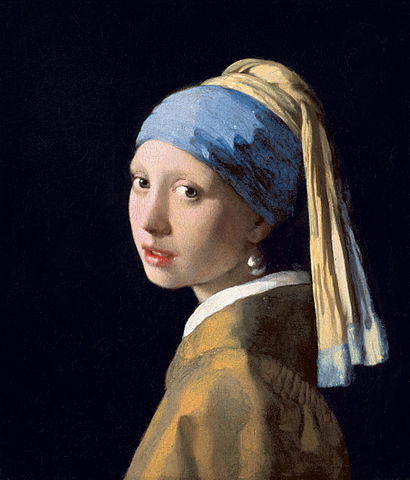
\includegraphics[trim=0 0 0 0,clip,height=.3\hsize]{./img/410px-Meisje_met_de_parel.jpg}}}
    \put(157,183){\fbox{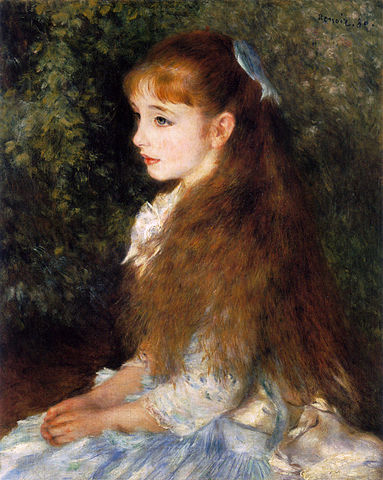
\includegraphics[trim=0 0 0 .4,clip,height=.3\hsize]{./img/MlleIreneCahen.jpg}}}
    % \put(155,184){\fbox{\includegraphics[trim=0 0 0 .4,clip,width=0.3\hsize]{429px-Mary_Lemon_Waller_-_Spring_Voices_royalacademyillu1896roya_0070.jpg}}}
    \put(257,183){\fbox{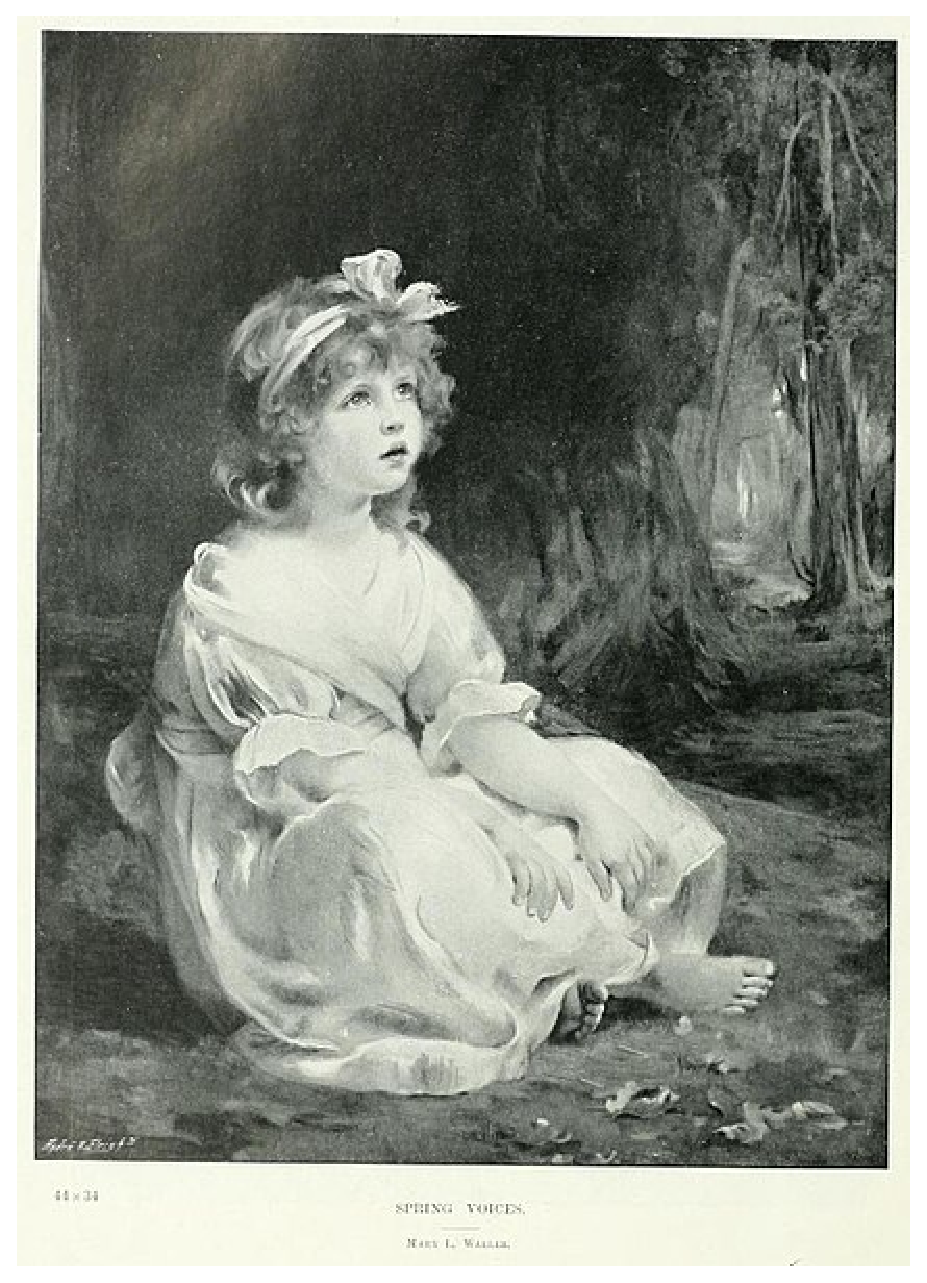
\includegraphics[trim=60 80 60 30,clip,height=.3\hsize]{./img/MaryLemon.eps}}}
\else
    \put(15,184){
\includegraphics[trim=0 0 0 0,clip,width=1.35\hsize]{./img/nipper.eps}}%VOLONE
\fi%VOLFOUR すべての表紙を見せる時


    % \put(150,180){\framebox(503,287){}}
    \put( 50,550){\timestamp}
    \put( 0,475){\linethickness{0.4mm}\line(1,0){600}}
    \put( 0,173){\linethickness{0.4mm}\line(1,0){600}}
\ifEnglish
%      \put( 50,528){\scalefont{1.8}\bfseries Ten Sentences A Day (T.S.A.D)}
      \put( 50,528){\scalefont{1.8}\bfseries Dictation for Every Day (D4E)}
\ifVOLONE
%      \put( 50,505){\scalefont{1.8}\bfseries Ten Sentences A Day: Volume 1}
\fi%VOLONE
\ifVOLTWO
%      \put( 50,505){\scalefont{1.8}\bfseries Ten Sentences A Day: Volume 2}
%      \put( 50,505){\scalefont{1.8}\bfseries Ten Sentences A Day: Volume 1 and 2}
\fi%VOLTWO
\ifVOLTHREE
%      \put( 50,505){\scalefont{1.8}\bfseries Ten Sentences A Day: Volume 1, 2, and 3}
\fi%VOLTHREE
\ifVOLFOUR
      \put( 50,505){\scalefont{1.8}\bfseries Ten Sentences A Day: Volume 1, 2, 3, and 4}
\fi%VOLFOUR
      \put( 50,484){\scalefont{1.5}\bfseries Let's learn Japanese through Dictation}
      % \put(210,450){\scalefont{3.0} Workbook}
      \put( 50,145){\scalefont{2.0}\bfseries Hilofumi Yamamoto}
      \put( 50,130){\itshape\bfseries Ph.\,D.\,in Linguistics}
      % \put( 50,100){\includegraphics[trim=10 45 10 45, clip, width=12mm]{./edx-logo.eps}}
      % \put( 90,104){\scalefont{1.5}\itshape\bfseries Tokyo\,Tech\,X}
      % \put( 50, 65){\fcolorbox{white}{royalblue}{\includegraphics[width=35mm]{../phd/logo02.png}}}
      \put( 50, 80){\fbox{
\includegraphics[width=35mm]{./img/tokyotechlogo/symbol_pdf_ja_180704/シンボルマーク+ロゴタイプ和文英文左右.pdf}}}
      \put(170,80){
\includegraphics[trim=0 0 0 0,clip,width=.14\hsize]{./img/titech12.pdf}}
      \put(225,80){
\includegraphics[trim=0 0 0 0,clip,width=.14\hsize]{./img/d4e.pdf}}
      \put(280,80){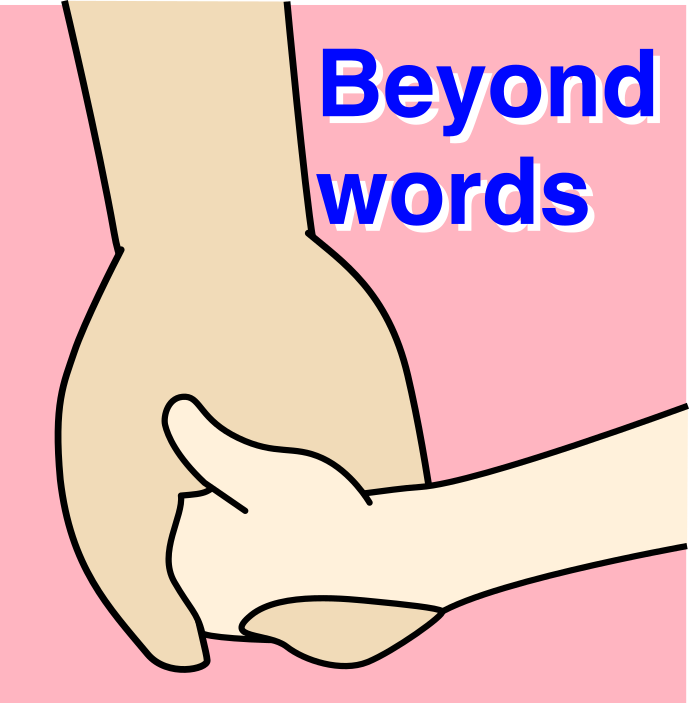
\includegraphics[trim=0 0 0 0,clip,width=.14\hsize]{./img/beyondwords.png}}
    \else
      \put(150,616){\scalefont{2.5}\bfseries Micro:bit Japanese}
      \put(195,600){\scalefont{1}\bfseries with dictation and shadowing}
      \put(200,580){\scalefont{1.5}\bfseries 作って学ぶアプローチ}
      \put(180,550){\scalefont{3.0} ワークブック}
      \put(202,162){\scalefont{0.8}\bfseries やま}
      \put(239,162){\scalefont{0.8}\bfseries もと}
      \put(275,162){\scalefont{0.8}\bfseries ひろ}
      \put(312,162){\scalefont{0.8}\bfseries ふみ}
      \put(200,145){\scalefont{2.0}\bfseries 山　元　啓　史}
      \put(215,130){\itshape\bfseries Ph.\,D.\,in Linguistics}

    \fi
  \end{picture}
  \newpage

  \ifEnglish
    Ten Sentences A Day: Dictation For Every Day (D4E)
  \else
    1日10文: 毎日学ぶディクテーション
  \fi

  \setlength\unitlength{1pt}
  \begin{picture}(0,130)(60,100)
    \put(63,60){
\includegraphics[width=.5\hsize]{./img/nipper.eps}}
    \put(60,57){\framebox(191,110){}}
    \put(255,57){
\includegraphics[width=5mm]{./img/Cc-public_domain_mark_white.eps}}
    \ifEnglish
      %One of the most famous late 19th and early 20th-century advertising icons was, apparently, a Jack Russell terrier, the very same one who was a model for a painting called “His Master’s Voice.”
      %The image was the foundation of the logo for many gramophone and recording brands like HMV, EMI, RCA, Victor Talking Machine Company, and more. The curious dog which looks and listens to the gramophone goes by the name of Nipper.
      %Nipper (1884–1895) was born in Bristol, England, and was a mixed-breed Jack Russell Terrier. The playful dog’s tendency to bite the backs of visitors legs earned him the name.
      \put(55,40){\scalefont{1.5} ``His Master's Voice'' by \href{https://en.wikipedia.org/wiki/Francis_Barraud}{Francis Barraud (1856-1924)}}
      \put(60,26){\scalefont{1.0} It is the logo for many gramophone and recording brands like HMV, EMI, RCA.}
      \put(60,15){\scalefont{1.0} The curious dog which looks and {\bfseries listens} to the gramophone goes by the name of Nipper.}
      \put(60,04){\scalefont{1.0} \href{https://www.thevintagenews.com/2017/12/12/jack-russell-terrier-nipper/}{Jack Russell Terrier Nipper}}
    \else
      \put(60,30){\scalefont{1.0}富嶽三十六景、神奈川沖波裏 (1829--32頃): 葛飾北斎 (1760--1849)}
      \put(60,15){\scalefont{0.8}波の形は現実の波しぶきと同じ形をしていると言われている。}
    \fi
  \end{picture}

  \vfill

  \ifEnglish
    \begin{itemize}\small
      \item Production: Hilofumi Yamamoto
      \item Scenario writing: Hilofumi Yamamoto
      \item Programming: Hilofumi Yamamoto
      \item Recording Cast: Midori Komatsu, Mika Ebara, Ruri Kasahara, Kazunori Suzuki
      \item The typography was done in \upLaTeX.
      \item Vim and Neovim used for editing.
      \item Audacity used to edit the audio.[\href{https://www.audacityteam.org/}{\url{https://www.audacityteam.org/}}]
      \item JavaScript/PHP/superagent.js used for D4E web-app development.
    \end{itemize}
  \else
    \begin{itemize}\small
      \item 企画制作: 山元啓史
      \item シナリオ: 山元啓史
      \item プログラム開発: 山元啓史
      \item 録音出演: 小松翠、榎原実香、笠原瑠璃、鈴木一徳、山元啓史
      \item 組版は\upLaTeXを用いました。
      \item エディタは、Vim/Neovimを用いました。
      \item 音声の編集にはaudacityを使いました。
        [\href{https://www.audacityteam.org/}{\url{https://www.audacityteam.org/}}]
      \item JavaScript/PHP/superagent.js used for D4E web-app development.
    \end{itemize}
  \fi

  \noindent
  \begin{tabular}[t]{rl}
    \begin{minipage}[c]{24mm}
      \fbox{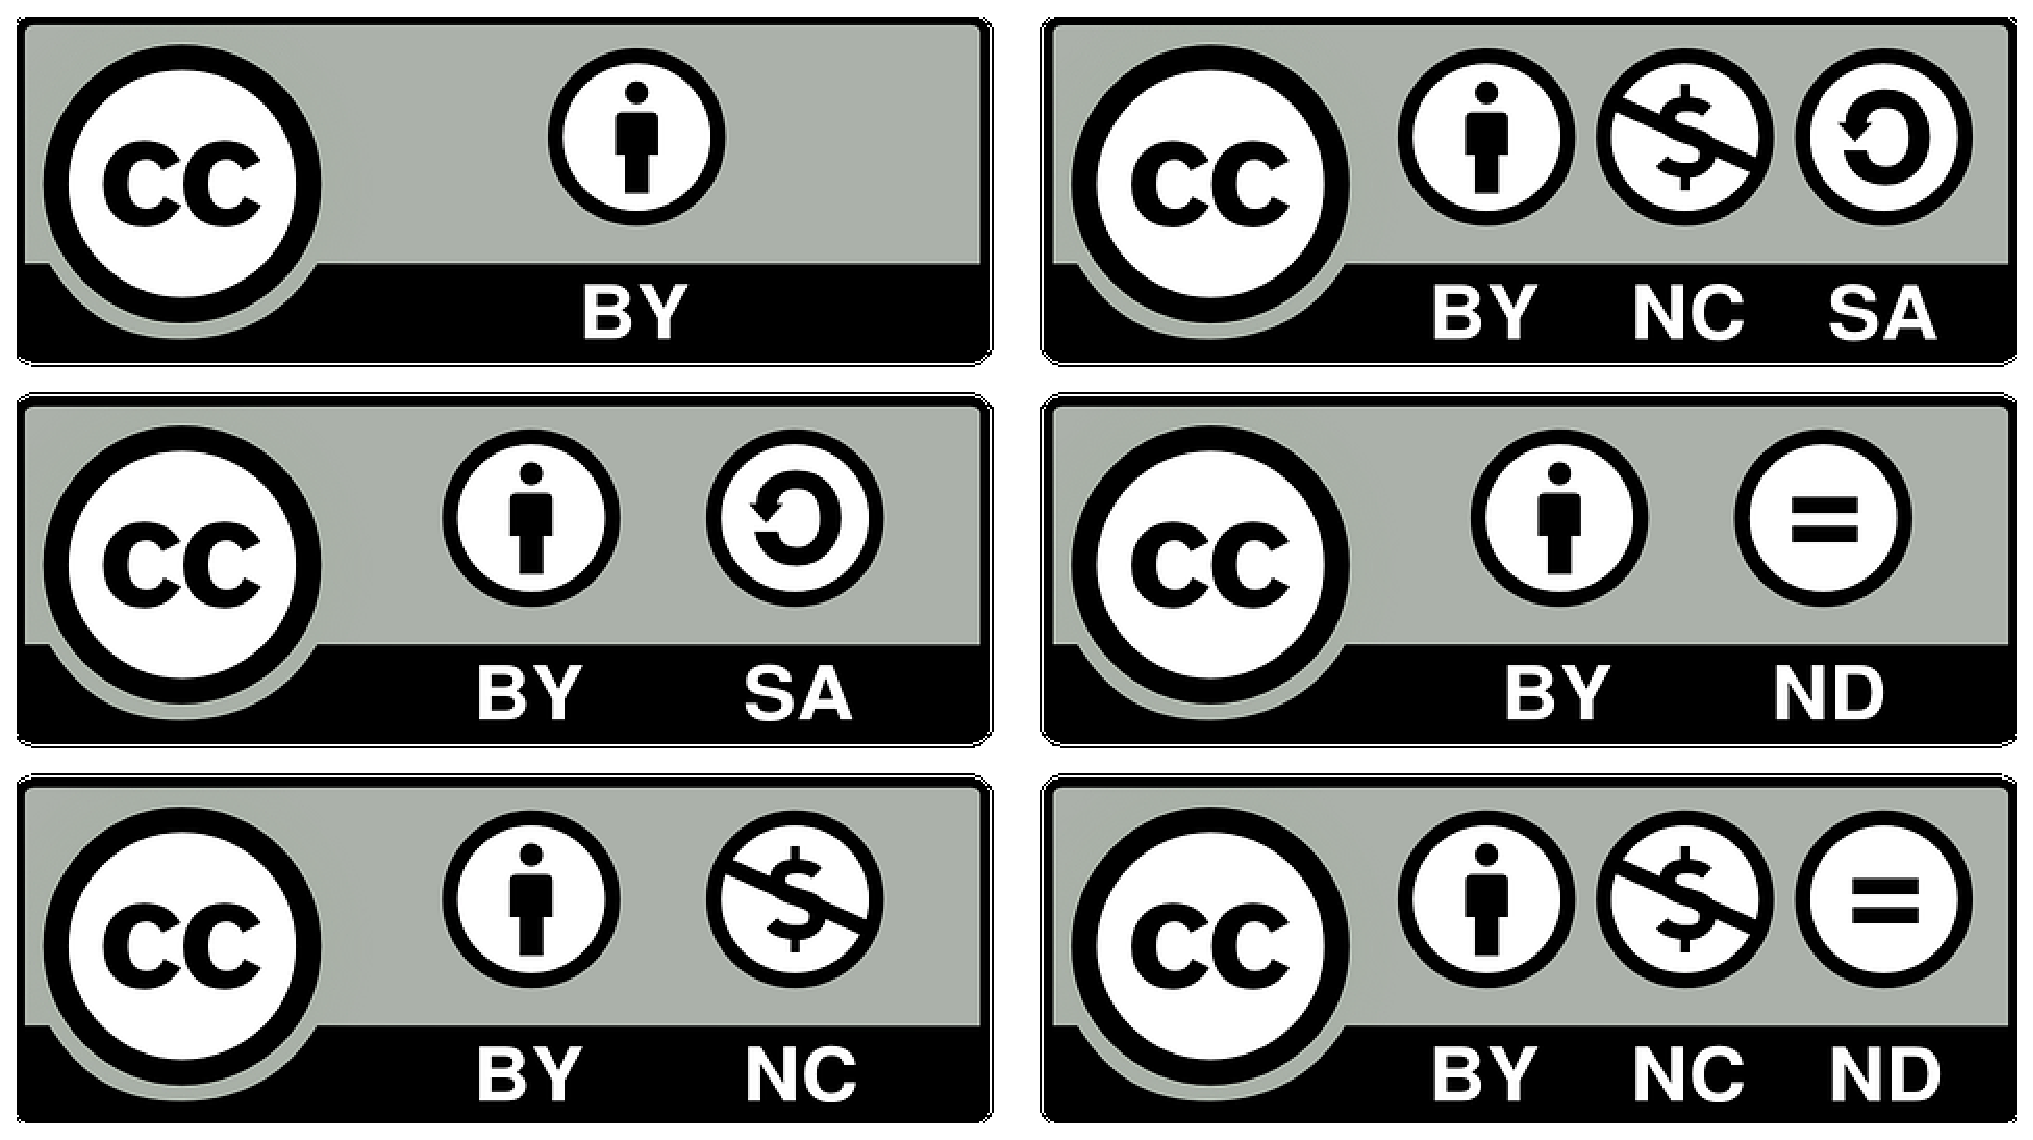
\includegraphics[trim=0 170 490 180,clip,width=20mm]{./img/cclicense.eps}}
    \end{minipage}
&
\begin{minipage}[c]{50mm}\footnotesize
  Hilofumi Yamamoto, Ph.D. \rule[-.0pt]{0pt}{8pt}
  \\
  Tokyo Institute of Technology
\end{minipage}
\\
  \end{tabular}

  %Hilofumi Yamamoto, Ph.\,D. in Linguistics, Tokyo Institute of Technology

  %\textcopyright\,Hilofumi Yamamoto, 2019

\end{frontmatter}

\ifEnglish
  \chapter*{Preface}
\else
  \chapter*{はじめに}
\fi

\ifEnglish
  %This is one of the Japanese textbooks by edX MOOCs Tokyo Institute of Technology Online Education Development Room.
  There are tips for studying a language.
  Don't care about the details.
  It is also necessary to get used to thinking that it doesn't matter.
  No matter how much you study the structure of a bicycle, you cannot ride a bicycle.
  Many people ride a bicycle without knowing the structure of the bicycle.
  You can't ride a bicycle just by looking at it.
  If you want to be able to ride a bicycle, just ride a bicycle.
  Let's do it anyway.
\else
  %本書はedX MOOCs 東京工業大学オンライン教育開発室による日本語の教科書である。
  言語の勉強にはコツがあります。
  詳細なところにこだわらないことである。
  どうでも良いと考えることに慣れることも必要である。
  自転車の構造をいくら勉強しても、自転車には乗れない。
  自転車の構造を知らないで自転車に乗っている人はたくさんいる。
  自転車を見ているだけでは、自転車に乗れない。
  とにかく自転車に乗らなければ、乗れるようにはなれない。
  やってみよう。
\fi

\vspace*{1\baselineskip}
\begin{flushright}
  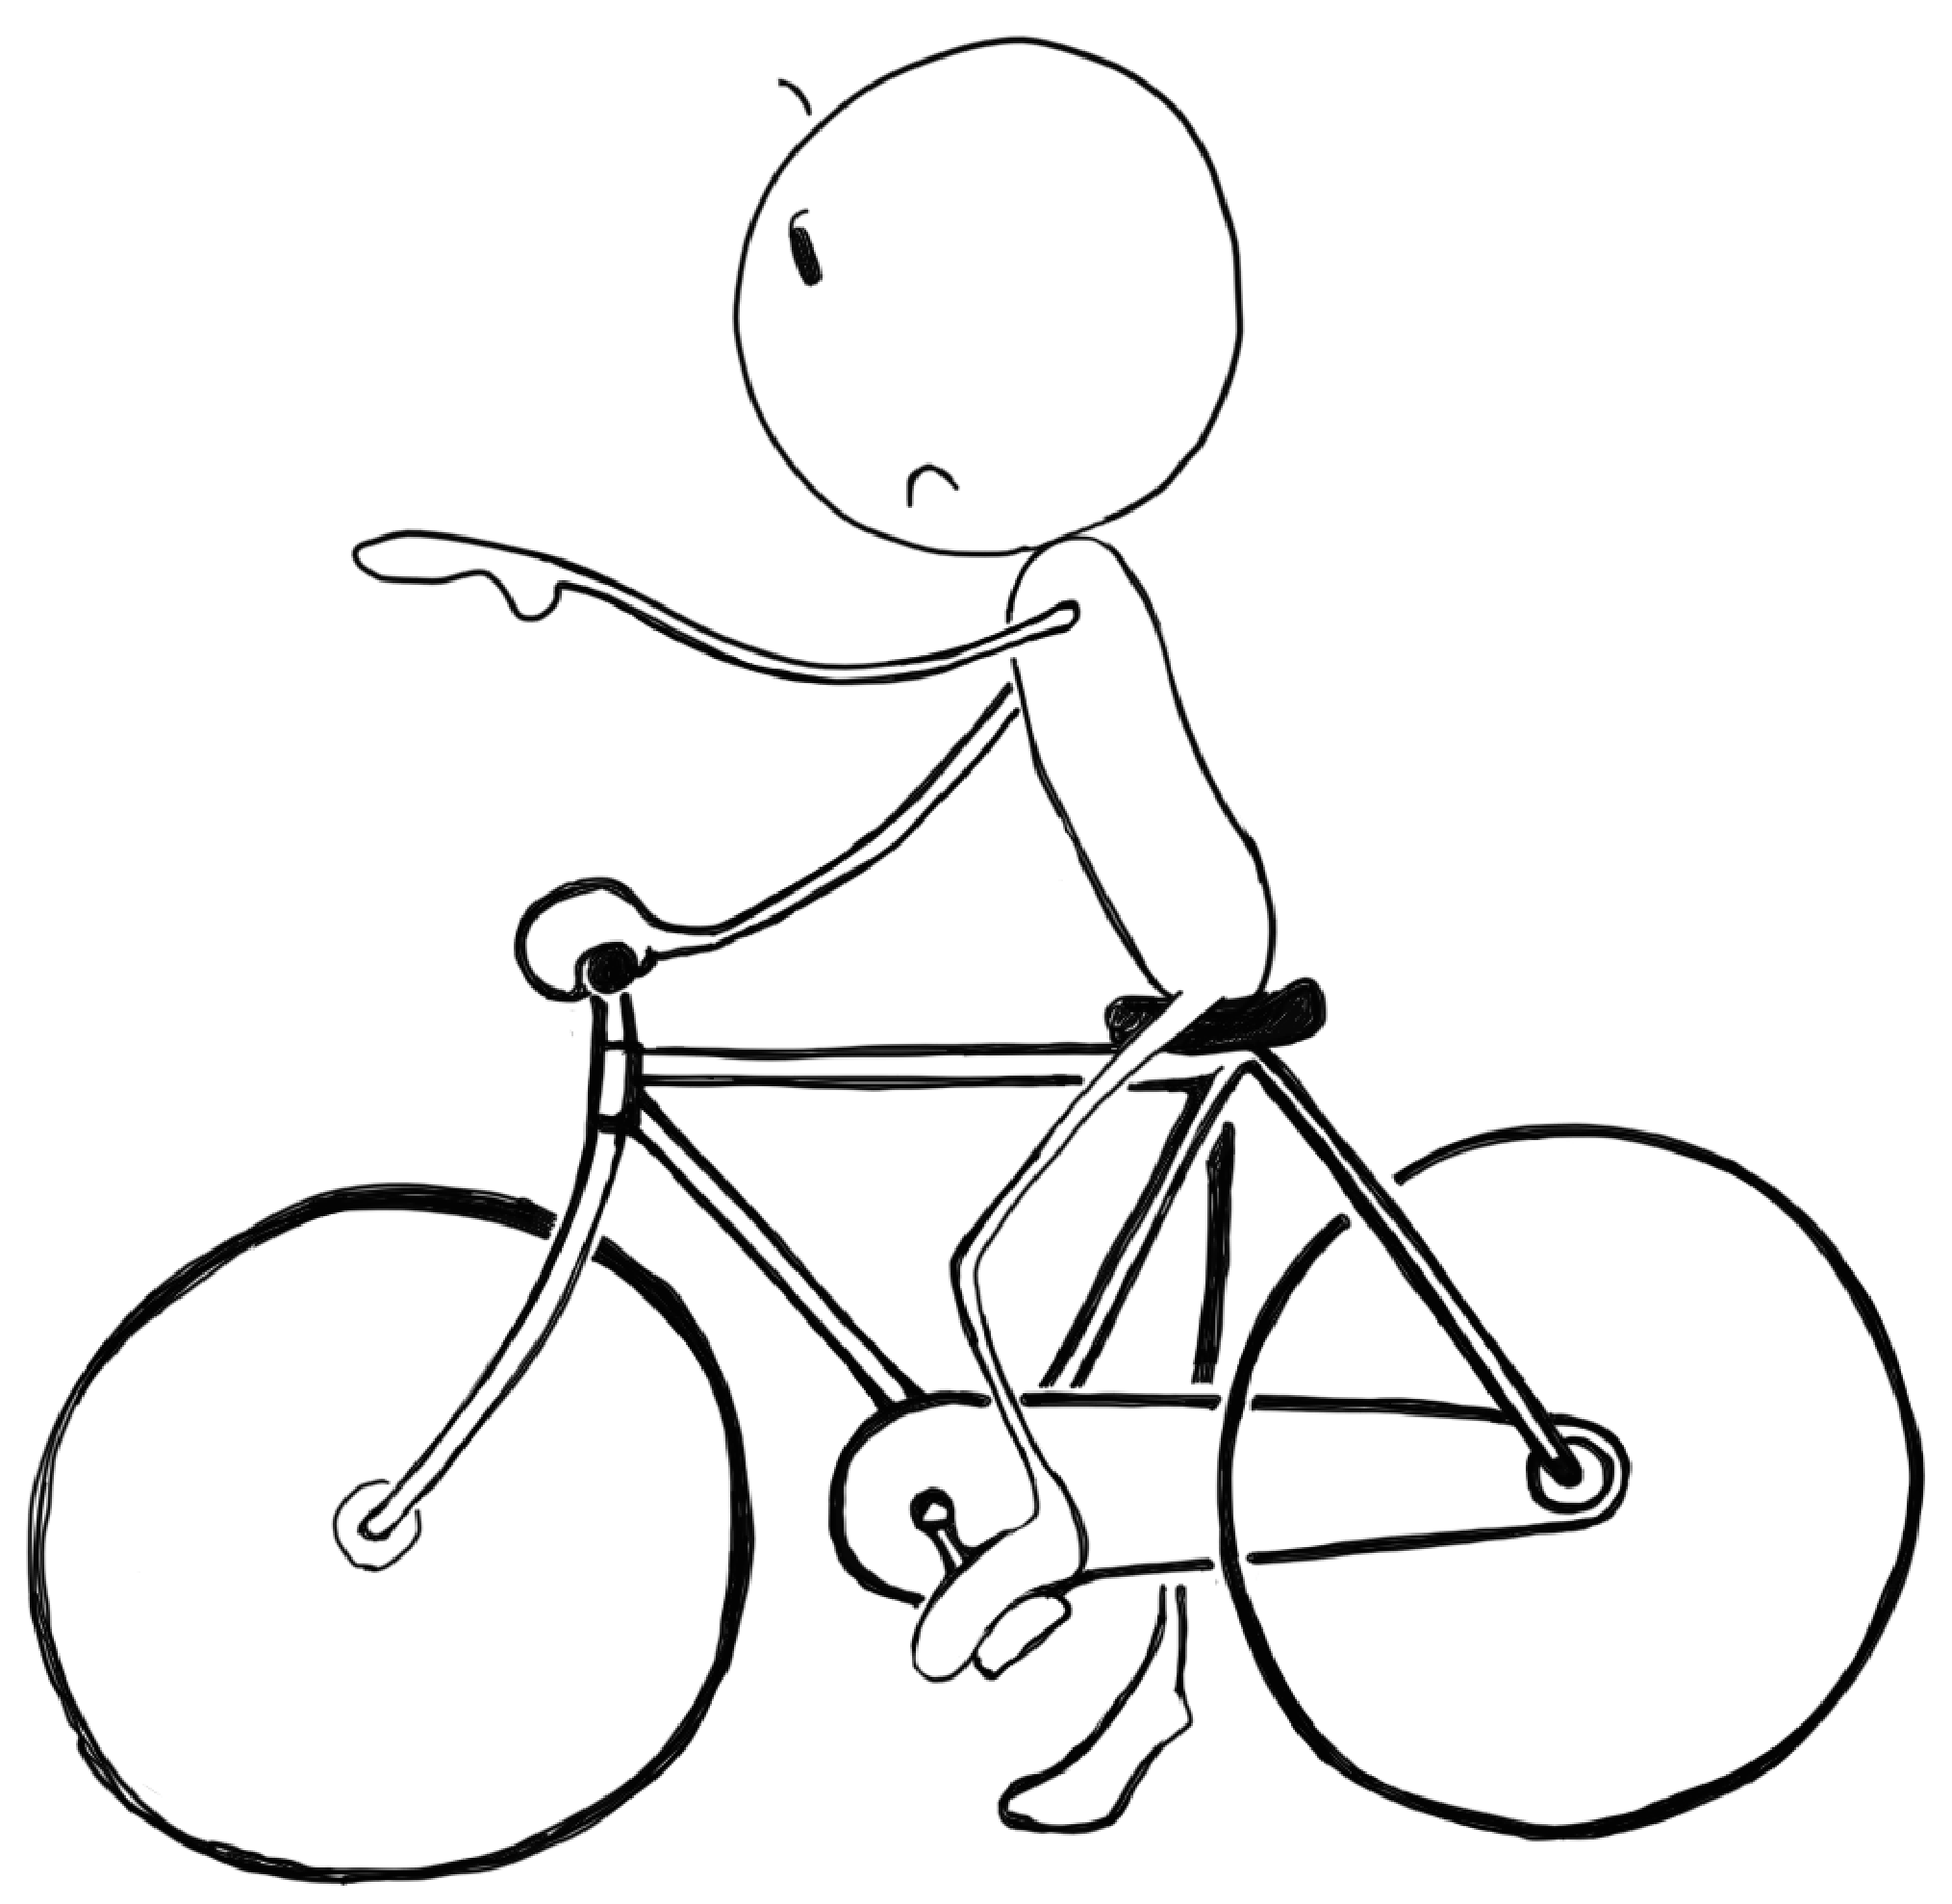
\includegraphics[width=.2\hsize]{./img/bicycle201801.pdf}

  \ifEnglish
    Hilofumi Yamamoto, Ph.\,D.\\
    Professor of Linguistics\\
    Tokyo Institute of Technology\\
  \else
    {\large 山 元 啓 史}\hspace*{3zw}

    {\small 東京工業大学教授\hspace*{2zw}}
  \fi
\end{flushright}

%\end{document} % for checking the first page.



\section*{Abbreviation}

\begin{multicols}{2}
  \begin{description}
    \item[1G] 1st group verb
    \item[2G] 2nd group verb
    \item[3G] 3rd group verb
    \item[adj] adjective
    \item[adv] adverb
    \item[archaic] archaic word
    \item[casual] casual style
    \item[causa] causative
    \item[col] colloquial expression
    \item[v.comp] compound verb
    \item[n.comp] compound noun
    \item[cond] conditional form
    \item[formal] formal style
    \item[GN] grammar notes
    \item[honor] an honorific form of verb,
    \item[i-adj] i-adjective
    \item[n] noun
    \item[na-adj] na-adjective
    \item[non-past] non past tense
    \item[nv] noun-verb (suru)
    \item[psiv] passive voice
    \item[past] past tense
    \item[pot] potential form
    \item[prefix] prefix
    \item[suffix] suffix
    \item[suru] suru verb
    \item[te-iru] te-iru
    \item[te-ita] te-iru
    \item[te-te] te-te
    \item[te-ta] te-ta
    \item[v.te] te-form of verb
    \item[v] verb
    \item[vi] intransit verb
    \item[voli] volitional form
    \item[vt] transit verb
  \end{description}
\end{multicols}


\setcounter{tocdepth}{2}
\tableofcontents
%\listoffigures
%\listoftables
%\lstlistoflistings

\mainmatter

\ifEnglish
  \chapter*{Getting Started}
\else
  \chapter*{さあ！はじめよう}
\fi

\ifEnglish
  The important thing is vocabulary.
  It is important to use various words.
  Each word has its own inevitable scene and sentence pattern.
  The sentence pattern has suitable scenes and words as well.
  Sentence patterns are not always available.
  That's why you shouldn't study sentence forms alone in the beginning.
\else
  重要なのは語彙である。
  いろいろな単語を使うのが重要だ。
  単語にはそれぞれに必然的な場面と文の形式がある。
  その文型にはふさわしい場面と単語がある。
  その文の形式が好きな時にいつでも使えるわけではない。
  それが文の形式だけをはじめに勉強してはいけない理由だ。
\fi

\ifEnglish
  \section*{Let's practice every day}

  First of all, it is important to practice every day.
  Let's do it again and again every day.
  Dictation is a very simple exercise of writing audible sounds and easy-to-follow activities.
  the method must be simple.
  If the content is of your favorite genre, you can listen and write whatever you want.
  Just choose your favorite genre of listening.
  Let's challenge and write as many times as possible.
  While listening again and again, you will become thinking about the reason why you cannot do it.
  This notion is called ``strategy.''
  In order to improve your language skills, you need to think about strategies by yourself.
  Because the strategy is different for each person to learn, it is important to find your own strategies.
  Dictation provides a very good opportunity to find the knack of being able to do it yourself.
  Again, I'll say it again.
  The way to dictate is for you to find out by yourself.

\else
  \section*{毎日練習しましょう}

  まず、毎日練習することが大切です。
  毎日、何度も何度もやりましょう。

  ディクテーションは、聞こえた音声を書き取るというとても単純な練習でやり方がわかりやすい活動です。
  いろいろな学習活動がありますが、方法が簡単であることはとても重要です。
  好きなジャンルの内容であれば、何でも聞いて書き取ればいいので、材料選びも簡単です。
  何度でも挑戦して書き取りましょう。
  何度も聞いているうちに、自分ができない理由を考えて工夫をするようになります。
  この工夫をストラテジーと言います。
  語学を上達するためには、自分でストラテジーを考えて勉強の工夫をする必要があります。
  ストラテジーは学ぶ人それぞれによって違うものですから、自分でやることが重要です。
  ちょうど自転車に乗る練習をするときに、体重をどちらに向けるか、いつペダルに力を入れるか、など本人にしかわからないことがたくさんあります。
  みんなと同じ練習をしてもよいのですが、自分で実際にやって自分で工夫する、自分のストラテジーを身につける必要があります。
  ディクテーションは自分で自分ができるようになるコツを見つけるとてもよいチャンスを提供してくれます。
  もう一度いいます。
  ディクテーションの方法は自分自身で見つけることです。
\fi

\ifEnglish
  \section*{Listen to what you like and write}

  It is important to definitely listen to the contents of the script.
  Nowadays, it's very convenient because many of YouTube video footages have subtitles in various language recently.
  After seeing the subtitle, it is a very good way to repeat the phrases, without looking at subtitles.
  It is also a good way to write immediately without looking at subtitles.
  Both are a good way, but choosing what you like most.
  No matter how difficult it is, if it is your favorite content, it is worth trying to catch it.
  Please feel free to write with your wild guess while thinking ``It might be said such a thing.''
  Easiness is different from person to person.
  Rather than easiness, you should choose what you like.
  If you feel it is difficult, choose short ones and listen.
  Even short ones can be difficult.
  However, you can identify where it is difficult.
  The difficulty is often caused by not being aware of the content itself of a word even though the word itself is simple and easy to understand.
  That's why there is something you do not understand even if you look up the dictionary even no matter how many times you listen.
  It is important to hear what you are interested in the content.

\else
  \section*{好きな内容を聞いて書いてみる}

  確実にスクリプトのある内容を聞くことが大切ですが、いまはYouTubeに字幕がありますので、とても便利です。
  字幕を見た後、字幕を見ないで、思い出して書くのもとても良い方法です。
  また字幕を見ないで、すぐに書いてみるのも良い方法です。
  どちらも良い方法ですが、自分の好きな内容を選ぶことです。
  自分の好きな内容であれば、どんなに難しそうでもかまいません。
  どうぞ「こんなことをいっているのかもしれない」と思いながら、ヤマカンで書いても構いません。
  やさしいというのは人によって違います。
  やさしいものというよりも、自分の好きなものを選びましょう。
  あなたがそれが難しいと感じるならば、短いものを選んで聞いてください。
  短いものでも難しい場合があります。
  しかし、どこが難しいかを特定できます。
  その難しさは、単語自体は優しくても、単語が示す内容そのものを知らないことが原因であることが多いのです。
  辞書を調べても、何回聞いてもわからないことがあるのはそのためです。
  内容に興味が持てるものを聞き取るのが重要です。
\fi

\ifEnglish
  \section*{Listen to the sentences of your favorite genres}

  At the beginning, let's write without looking at the workbook.
  Let's write the sentence little by little after listening.
  Since every sentence is a short sentence, please press the Play button and listen again and again.
  In the same way, choose your favorite program and let's write short sentences.
  You can choose your favorite program, favorite content.
  If you are studying mathematics, it is good way for you to choose a YouTube program in mathematics which you can understand the content.
  Also, if your hobby is gardening, it would be a nice way to choose a video about gardening.
  When one listens to something, one would not listen to things that are not related to oneself.
  Let's think about what you are interested in the first place.

\else
  \section*{好きなジャンルの文を聞く}

  はじめは、ワークブックを見ないで書きましょう。
  聞いてから、文を少しずつ書きましょう。
  どの文も短い文ですから、Playボタンを押して、何度でも聞き直してください。
  同じ方法で、自分で好きな番組を選んで、短い文の書き取りをやってみましょう。
  好きな番組、好きな内容を選ぶとよいでしょう。
  もし、あなたが数学を勉強しているのであれば、内容がわかる範囲の数学のYouTubeの番組を選ぶと良いでしょう。
  また、あなたの趣味がガーデニングであるならば、ガーデニングに関するビデオを選ぶのはいい方法でしょう。
  人間が何かを聞くとき、自分とは関係のないものは聞かないはずです。
  自分の興味ある内容を、第一に考えて選びましょう。

\fi

\ifEnglish
  \section*{Write as you heard}

  You write down the sentences that you heard several times.
  Even if you do not know the spelling of words you just listened, you should spell the sentence out.
  Since it is not a test, you can type it out with checking the spelling using a dictionary.
  I think there are cases where unknown words come out.
  There is something that you do not absolutely know what you are going to hear.
  You do not mind listen it over and over again until you give it up.
  It is also important to check whether sentences you write down grammatically are correct.
  While watching the completed sentence, listen to the sentence again and fix it if necessary.


\else
  \section*{聞いたとおりに書け}

  数回聞いて覚えた文を書きだします。
  単語がわからなくても、間違っていても構わず書きます。
  テストではないので、辞書を使ってスペルを確認しながら書き出しても構いません。
  知らない単語が出てくる場合もあると思います。
  どうしても何を言っているのかわからないということもあるはずです。
  これ以上は、どうしてもわからないというまで、何度聞き直しても構いません。
  何度聞いてもわからなかった箇所は、後でなぜ聞き取れなかったのか復習しやすいようにしておきましょう。
  書いた文が文法的に成り立っているかを確認することも大切なことです。
  完成した文を見ながら、もう一度通して文を聞き、必要なら修正します。

\fi

\ifEnglish
  \section*{Scoring and Feedback}

  If you can hear it but you misspelled it, you only have to learn the spelling.
  However, in dictation, there are times when you mistakenly write by listening to similar words.
  There are also sounds which you skip to write since you fail to hear them.
  In addition, there are times when multiple words are connected and it is not easy to know where the boundary of a word is.
  In listening exercises that just listened to with your ears, you remain vague and you can not clearly see what you could not do.
  However, as a dictation, you will actually understand clearly where you cannot do it.
  For example, if you missed the preposition, you could not hear the change, such as the connection of the sound, it is merely one of the reasons.

\else
  \section*{採点とフィードバック}

  聞き取れたけれどスペルを間違えたのなら、スペルを覚えれば良いのです。
  しかし、ディクテーションでは、似ている単語を聞き間違えて書いていることがあります。
  また、聞き取れずに抜かしている音もあります。
  さらに、複数の単語が繋がって、どこが単語の境目だかわからなからないこともあります。
  単に耳で聞いただけのリスニング練習では、あいまいなままで、はっきり自分のできなかったところがわかりません。
  しかし、ディクテーションとして実際に書いてみると自分のできないところがハッキリわかります。
  例えば、前置詞を聞き逃していた場合、音の繋がりなどの変化を聞き取れなかったことも理由の一つです。

\fi

\ifEnglish
  \section*{Exchange of opinions}

  The system will sometimes show sentences which you could not write properly before, and you will review those sentences again.
  Please try reading aloud by shadowing, reciting, etc.
  After daily dictation, there is a questionnaire.
  Please inquire about where it was difficult, what could not be done, how can you do it?

\else
  \section*{意見交換}

  回答の合間にかつて間違えた文もときどき再び出題されます。
  シャドーイング、暗唱などで音読もしてみてください。
  毎日のディクテーションの後に、アンケートがあります。
  どこが難しかったのか、何ができなかったのか、どうしたらできるようになるのか、などを質問してください。

\fi

\ifEnglish
  \section*{How to use software}
  \begin{enumerate}
    \item Visit URL: \href{https://cuckoo.js.ila.titech.ac.jp/~yamagen/d4ev5/}{https://cuckoo.js.ila.titech.ac.jp/~yamagen/d4ev5/}
    \item Log in the site with TokyoTech's m-address and JCOS password.
    \item The list of practice episodes will be shown. Choose the episode you want to practice.
    \item Japanese input system and language-specific input system is not required. Please enter directly in the Roman alphabet.
    \item By pressing the ENTER key, practice will start.
    \item If you want to hear the sound once again, please press the ESC key or the speaker icon.
    \item You can check the answer by pressing the ENTER key.
    \item You will be given the correct answer for each hiragana. Incorrect hiragana is marked with a question mark.
    \item If you want to stop practicing midway, press the "QUIT" button.
    \item The amount of daily practice is shown in the performance summary.
  \end{enumerate}
\else
  \section*{ソフトウェアの使い方}
  \begin{enumerate}
    \item URL: \href{https://cuckoo.js.ila.titech.ac.jp/~yamagen/dictee/}{https://cuckoo.js.ila.titech.ac.jp/~yamagen/dictee/}に行ってください。
    \item 東京工業大学のmアドレスとJCOSのパスワードで上記のサイトにログインしてください。
    \item 練習のエピソード一覧がありますので、練習したいエピソードを選んでください。
    \item 日本語入力システムや言語特有の入力システムは不要です。直接ローマ字で入力してください。
    \item ENTERキーを押すと練習が始まります。
    \item もう一度、音声を聞くときには、ESCキーまたはスピーカアイコンを押してください。
    \item ENTERキーを押すと答えがチェックできます。
    \item ひらがな毎に正解が示されます。間違っているひらがなは「？」で示されます。
    \item 練習を途中でやめたいときには「QUIT」ボタンを押します。
    \item 毎日の練習量は、パフォーマンス集計で示されます。
  \end{enumerate}
\fi

\begin{figure}[htb]\centering\small
  \fbox{\includegraphics[trim=0 0 0 0,clip,width=.97\hsize,angle=00]
  %{./d4e-screen01.pdf}}
  {./img/d4eLoginScreen.png}}
  \caption{Log in screen}
\end{figure}

\begin{figure}[htb]\centering\small
  \fbox{\includegraphics[trim=0 0 0 0,clip,width=.8\hsize]
%  {./d4e-screen02.pdf}}
  {./img/d4eEpisodeMenu.png}}
  \caption{Episode Menu}
\end{figure}

\vspace*{-2\baselineskip}

\begin{figure}[htb]\centering\small
  \fbox{\includegraphics[trim=0 0 0 0,clip,width=.8\hsize]
  %{./d4e-screen03.pdf}}
  {./img/d4eInstruction.png}}
  \caption{Instruction and practice screen}
\end{figure}

\vspace*{-2\baselineskip}

\begin{figure}[htb]\centering\small
  \fbox{\includegraphics[trim=0 0 0 0,clip,width=.8\hsize]
  %{./d4e-screen04.pdf}}
  {./img/d4eRomajiTyping.png}}
  \caption{Romaji typing}
\end{figure}

\vspace*{-2\baselineskip}

\begin{figure}[htb]\centering\small
  \fbox{\includegraphics[trim=0 0 0 0,clip,width=.8\hsize]
  %{./d4e-screen05.pdf}}
  {./img/d4eCheckAnswer.png}}
  \caption{Checking an answer}
\end{figure}

\vspace*{-2\baselineskip}

\begin{figure}[htb]\centering\small
  \fbox{\includegraphics[trim=0 0 0 0,clip,width=.8\hsize]
  %{./d4e-screen06.pdf}}
  {./img/d4eSuccessNext.png}}
  \caption{Success and the next question}
\end{figure}

\vspace*{-2\baselineskip}

\begin{figure}[htb]\centering\small
  \fbox{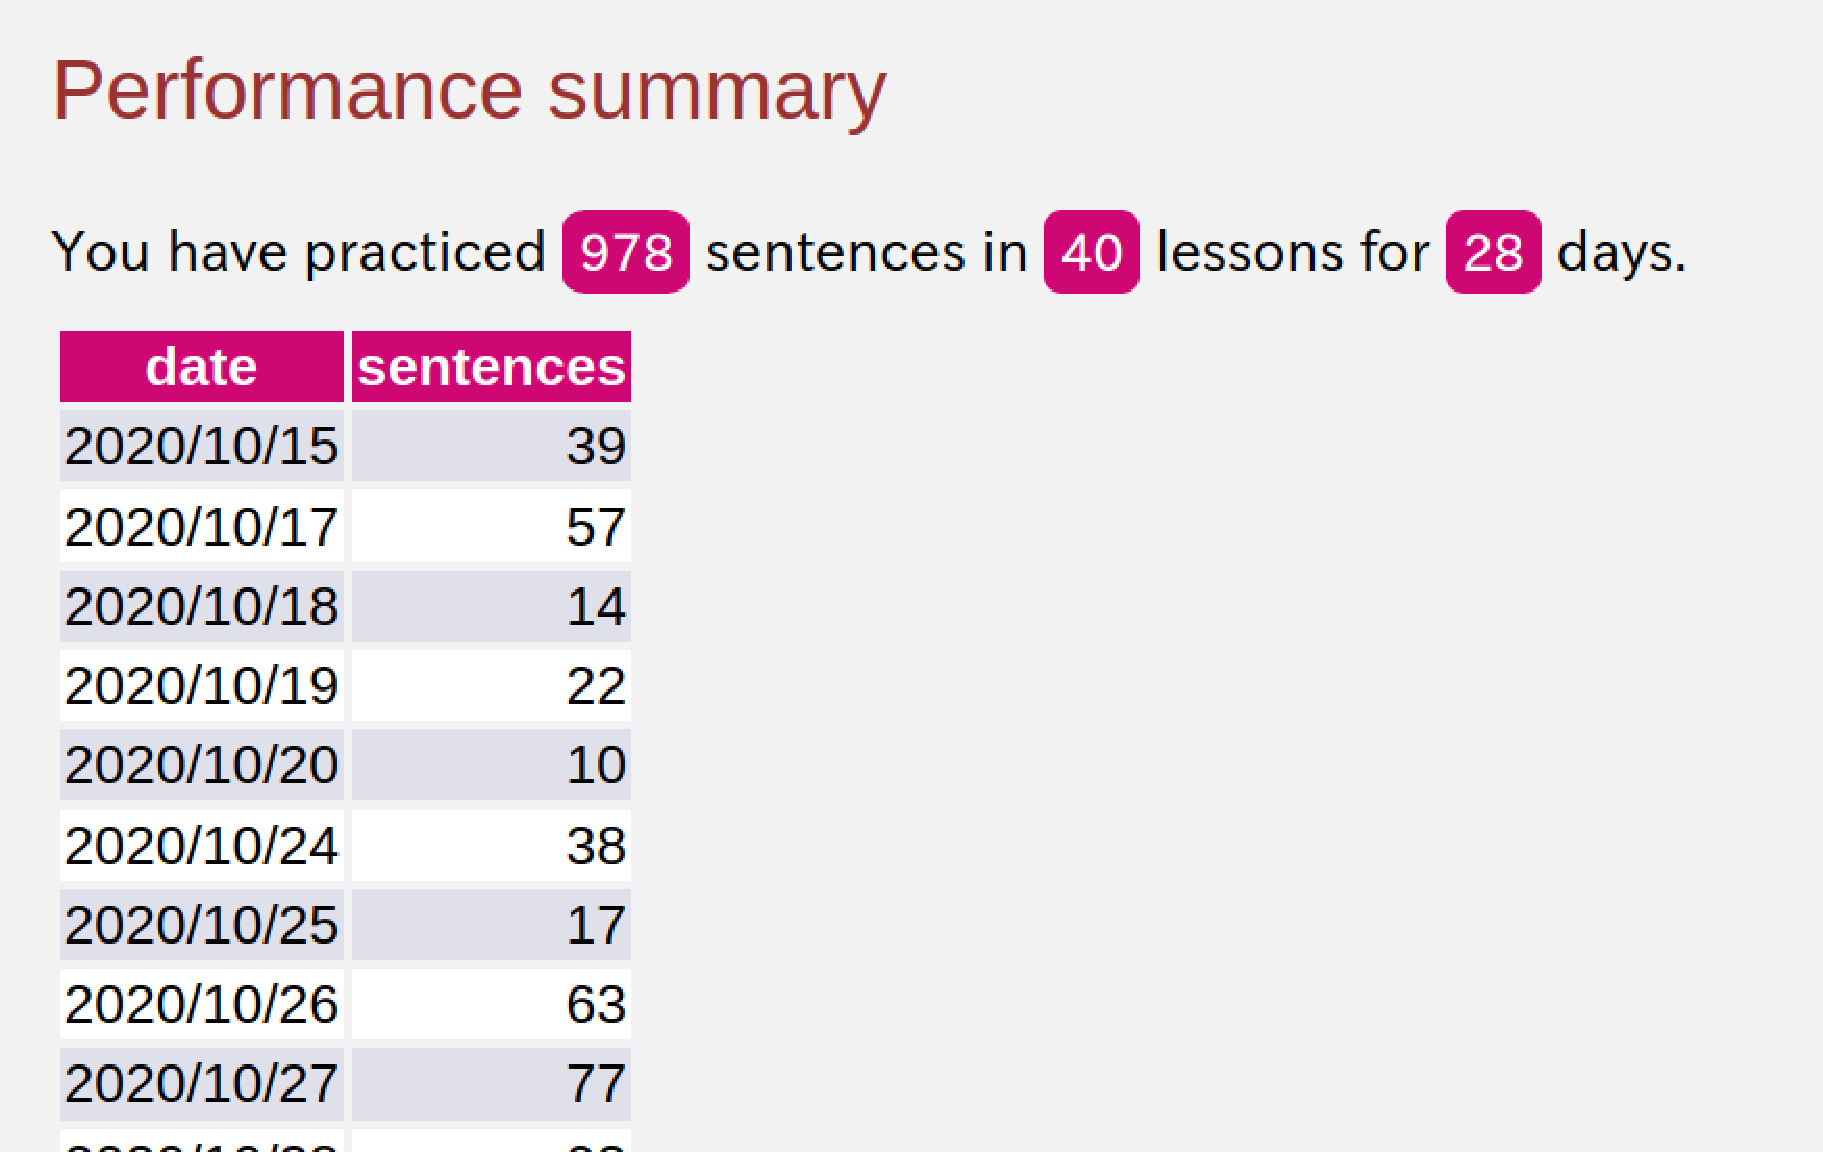
\includegraphics[trim=0 0 0 0,clip,width=.8\hsize]{./img/d4e-screen07.pdf}}
  \caption{Performance summary}
\end{figure}

%%%%%%%%%%%%%%%%%%%%%%%%%%%%%%%%%%%%%%%%%%%%%%
%%   Dictation   %%%%%%%%%%%%%%%%%%%%%%%%%%%%%
%%%%%%%%%%%%%%%%%%%%%%%%%%%%%%%%%%%%%%%%%%%%%%
\ifVOLONE
\ifEnglish
  \chapter{Textbook: Volume 1}

  The important thing you should do is to keep practicing everyday.
  If you keep it doing, you will come to regard it as a habit.
  And finally you will become not to have even any consciousness that you are using language.
  Type it as you hear according to the video footages with English captions.

\else
  \chapter{Textbook: Volume 1}

  あなたがすべき重要なことは、毎日練習し続けることです。
  あなたがそれをやり続けるなら、あなたはそれを習慣と見なすようになるでしょう。
  そして最後に、あなたは言葉を使っているという意識さえ持っていないようになるでしょう。
  英語のキャプション付きのビデオ映像に従って入力しましょう。

\fi

%\newpage
\ifEnglish
  \section{Week 1: Phatic Communion}%E
\else
  \section{Week 1: ファティーク}%J
\fi%English

\ifEnglish
  Phatic communion is one of the fundamental functions of language and an indispensable notion of communication as well.
\else
  ファティーク・コミュニオンは、言語の基本的な機能の1つであり、コミュニケーションの不可欠な概念でもあります。
\fi

%\newpage
\ifEnglish
  \subsection{Day 1: Greetings}%E
%D4E%day:001
%D4E%title:Greetings
\else
  \subsection{Day 1: あいさつ}%J
\fi%English
%\subsubsection{Objectives}

\ifEnglish
  Greeting is the most basic word to build interpersonal relationships.
  If you do not greet, you will be in a quite bad situation.
  Energetically pleasant, let's greet.
  You surely can start a good human relationship.
\else
  あいさつは対人関係を作り上げるために最も基本的なことばです。
  あいさつをしないととても険悪な状況になることも多いのです。
  元気に気持ちよく、あいさつをしましょう。
  きっと良い人間関係を始められるはずです。
\fi

\subsubsection{Sentences}
\begin{enumerate}
  \ifWB
  \item A: \ruby{田中}{たなか}です。\underline{\hspace{6em}}。\mySound{00101}\\I am Tanaka. Nice to meet you.%はじめまして%1-1-1-DB
  \else
  \item A: \ruby{田中}{たなか}です。\underline{はじめまして}。\mySound{00101}\\I am Tanaka. Nice to meet you.%はじめまして%1-1-1-DB
  \fi%WB
%D4E%ID:1
%D4E%sentence:A: (田中:たなか)です。<BLANK>。
%D4E%english:I am Tanaka. Nice to meet you.
%D4E%answer:はじめまして
%D4E%model:はじめまして
%D4E%roman:hajimemashite
%D4E%notes:@D4E:greetings@
  \ifWB
  \item B: ジョンです。\underline{\hspace{6em}}。\mySound{00102}\\I am John. Nice to meet you.%どうぞよろしく%1-1-2-DB
  \else
  \item B: ジョンです。\underline{どうぞよろしく}。\mySound{00102}\\I am John. Nice to meet you.%どうぞよろしく%1-1-2-DB
  \fi%WB
%D4E%ID:2
%D4E%sentence:B: (ジョン:じょん)です。<BLANK>。
%D4E%english:I am John. Nice to meet you.
%D4E%answer:どうぞよろしく
%D4E%model:どうぞよろしく
%D4E%roman:douzoyoroshiku
%D4E%notes:
  \ifWB
  \item A: \underline{\hspace{6em}}は。\mySound{00103}\\Where are you from?%おくに%1-1-3-DB
  \else
  \item A: \underline{お\ruby{国}{くに}}は。\mySound{00103}\\Where are you from?%おくに%1-1-3-DB
  \fi%WB
%D4E%ID:3
%D4E%sentence:A: <BLANK>。
%D4E%english:Where are you from?
%D4E%answer:おくには
%D4E%model:お国は
%D4E%roman:okuniha
%D4E%notes:
  \ifWB
  \item B: \underline{\hspace{6em}}。\mySound{00104}\\I am from the UK.%イギリスからきました%1-1-4-DB
  \else
  \item B: \underline{イギリスからきました}。\mySound{00104}\\I am from the UK.%イギリスからきました%1-1-4-DB
  \fi%WB
%D4E%ID:4
%D4E%sentence:B: <BLANK>。
%D4E%english:I am from the UK.
%D4E%answer:イギリスからきました
%D4E%model:イギリスから来ました
%D4E%roman:(katakana)igirisu(hiragana)karakimashita
  \ifWB
  \item A: \underline{\hspace{6em}}。\mySound{00105}\\Good morning.%おはよう%1-1-5-DB
  \else
  \item A: \underline{おはよう}。\mySound{00105}\\Good morning.%おはよう%1-1-5-DB
  \fi%WB
%D4E%ID:5
%D4E%sentence:A: <BLANK>。
%D4E%english:Good morning.
%D4E%answer:おはよう
%D4E%model:おはよう
%D4E%roman:ohayou
  \ifWB
  \item B: \underline{\hspace{6em}}。\mySound{00106}\\Good morning.%おはようございます%1-1-6-DB
  \else
  \item B: \underline{おはようございます}。\mySound{00106}\\Good morning.%おはようございます%1-1-6-DB
  \fi%WB
%D4E%ID:6
%D4E%sentence:B: <BLANK>。
%D4E%english:Good morning.
%D4E%answer:おはようございます
%D4E%model:おはようございます
%D4E%roman:ohayougozaimasu
  \ifWB
  \item A: \underline{\hspace{6em}}。\mySound{00107}\\I will excuse you.%しつれいします%1-1-7-DB
  \else
  \item A: \underline{失礼します}。\mySound{00107}\\I will excuse you.%しつれいします%1-1-7-DB
  \fi%WB
%D4E%ID:7
%D4E%sentence:A: <BLANK>。
%D4E%english:I will excuse you.
%D4E%answer:しつれいします
%D4E%model:失礼します
%D4E%roman:shitsureishimasu  
  \ifWB
  \item B: \underline{\hspace{6em}}。\mySound{00108}\\Good bye then.%じゃまた,じゃ、また%1-1-8-DB
  \else
  \item B: \underline{じゃ、また}。\mySound{00108}\\Good bye then.%じゃまた,じゃ、また%1-1-8-DB
  \fi%WB
%D4E%ID:8
%D4E%sentence:B: <BLANK>。
%D4E%english:Good bye then
%D4E%answer:じゃまた
%D4E%model:じゃまた
%D4E%roman:jamata
  \ifWB
  \item A: \underline{\hspace{6em}}。\mySound{00109}\\Thank you.%ありがとうございます%1-1-9-DB
  \else
  \item A: \underline{ありがとうございます}。\mySound{00109}\\Thank you.%ありがとうございます%1-1-9-DB
  \fi%WB
%D4E%ID:9
%D4E%sentence:A: <BLANK>。
%D4E%english:Thank you.
%D4E%answer:ありがとうございます
%D4E%model:ありがとうございます
%D4E%roman:arigatougozaimasu
  \ifWB
  \item B: \underline{\hspace{6em}}。\mySound{00110}\\Welcome.%どういたしまして%1-1-10-DB
  \else
  \item B: \underline{どういたしまして}。\mySound{00110}\\Welcome.%どういたしまして%1-1-10-DB
  \fi%WB
%D4E%ID:10,
%D4E%sentence:B: <BLANK>。
%D4E%english:Welcome.
%D4E%answer:どういたしまして
%D4E%model:どういたしまして
%D4E%roman:douitashimashite
\end{enumerate}


\subsubsection{Words and Expressions}

\begin{enumerate}
  \item Tanaka/Tanaka/personal name.pn/田中\index{Tanaka}
  \item desu/determinor.GN/です\index{desu}
  \item John(jonn)/John/ジョン\index{John}
  \item d\=ozo/please/どうぞ\index{douzo@d\=ozo}
  \item yoroshiku/nice-to-meet-you/よろしく\index{yoroshiku}
  \item o--/prefix.formal.GN/お--\index{o@o--}
  \item kuni/country/国\index{kuni}
  \item wa/p.topic.GN/は\index{wa(ha)}
  \item igirisu/United Kingdom/イギリス\index{igirisu}
  \item kara/from/から\index{kara}
  \item ohay\=o/good morning.casual/おはよう\index{ohay\=o}
  \item gozaimasu/suffix.formal.GN/ございます\index{gozaimasu}
  \item ja mata/good bye then/じゃ、また\index{ja mata}
  \item arigat\=o gozaimasu/thank you/ありがとうございます\index{arigat\=o gozaimasu}
  \item d\=oitashimashite/welcome/どういたしまして\index{douitashimashite@d\=oitashimashite}
\end{enumerate}

%\newpage
\ifEnglish
  \subsection{Day 2: Be invited and inviting}%E
%D4E%day:002
%D4E%title:Be invited and inviting
\else
  \subsection{Day 2: 招待する・招待される}%J
\fi%English

\ifEnglish
  Let's ask questions using invitation expressions.
\else
  誘いの表現を使って質問をしてみましょう。
\fi
\ifEnglish
  These expressions can be used independently.
\else
  これらの表現は独立して使うことができます。
\fi
\ifEnglish
  There are no conjugations of verbs at all.
\else
  動詞の活用もありません。
\fi
\ifEnglish
  You can use as it is.
\else
  そのまま使えます。
\fi
\ifEnglish
  Let's use it as soon as you encounter a scene that you can use.
\else
  使えそうな場面に出会ったら、すぐに使ってみましょう。
\fi

\subsubsection{Sentences}
\begin{enumerate}
  \ifWB
  \item A: これ、どうですか？ B: \underline{\hspace{6em}}。 \mySound{00201}\\A: How do you think about this? B: It is nice.%いいですねぇ,いいですねえ%1-2-1-DB
  \else
  \item A: これ、どうですか？ B: \underline{いいですねぇ}。 \mySound{00201}\\A: How do you think about this? B: It is nice.%いいですねぇ,いいですねえ%1-2-1-DB
  \fi%WB
%D4E%ID:1
%D4E%sentence:A: これ、どうですか？ B: <BLANK>。
%D4E%english:A: How do you think about this? B: It is nice.
%D4E%answer:いいですね
%D4E%model:いいですね
%D4E%roman:iidesune
  \ifWB
  \item A: もう、\ruby{一杯}{いっぱい}、どうですか？　B: ええ、\underline{\hspace{6em}}。\mySound{00202}\\A: How about one more drink? B: Yes, please.%おねがいします%1-2-1-DB
  \else
  \item A: もう、\ruby{一杯}{いっぱい}、どうですか？　B: ええ、\underline{おねがいします}。\mySound{00202}\\A: How about one more drink? B: Yes, please.%おねがいします%1-2-1-DB
  \fi%WB
%D4E%ID:2
%D4E%sentence:A: もう、(一杯:いっぱい)、どうですか？ B: ええ、<BLANK>。
%D4E%english:A: How about one more drink? B: Yes, please.
%D4E%answer:おねがいします
%D4E%model:お願いします
%D4E%roman:onegaishimasu
  \ifWB
  \item A: お\ruby{願}{ねが}いします。 B: ええ、\underline{\hspace{6em}}。\mySound{00203}\\A: Could you do this for me? B: Yes, my pleasure.%よろこんで%1-2-3-DB
  \else
  \item A: お\ruby{願}{ねが}いします。 B: ええ、\underline{よろこんで}。\mySound{00203}\\A: Could you do this for me? B: Yes, my pleasure.%よろこんで%1-2-3-DB
  \fi%WB
  \ifWB
\else
\fi%WB
%D4E%ID:3
%D4E%sentence:A: お(願:ねが)いします。 B: ええ、<BLANK>。
%D4E%english:A: Could you do this for me? B: Yes, my pleasure.
%D4E%answer:よろこんで
%D4E%model:喜んで
%D4E%roman:yorokonde
\ifWB
\item A: \ruby{来週}{らいしゅう}はどうですか？ B: \underline{\hspace{6em}}...。\mySound{00204}\\A: How about next week? B: Next week, it's kinda...%らいしゅうはちょっと%1-2-4-DB
\else
\item A: \ruby{来週}{らいしゅう}はどうですか？ B: \underline{\ruby{来週}{らいしゅう}はちょっと}...。\mySound{00204}\\A: How about next week? B: Next week, it's kinda...%らいしゅうはちょっと%1-2-4-DB
\fi%WB
%D4E%ID:4
%D4E%sentence:A: (来週:らいしゅう)はどうですか？ B: <BLANK>...。
%D4E%english:A: How about next week? B: Next week, it's kinda...
%D4E%answer:らいしゅうはちょっと
%D4E%model:来週はちょっと
%D4E%roman:raishuuhachotto
\ifWB
\item A: \ruby{来週}{らいしゅう}はどうですか？ B: ええ、\underline{\hspace{6em}}。\mySound{00205}\\A: How about next week? B: Well, I will go if I can go.%いけたらいきます%1-2-5-DB
\else
\item A: \ruby{来週}{らいしゅう}はどうですか？ B: ええ、\underline{\ruby{行}{い}けたらいきます}。\mySound{00205}\\A: How about next week? B: Well, I will go if I can go.%いけたらいきます%1-2-5-DB
\fi%WB
%D4E%ID:5
%D4E%sentence:A: (来週:らいしゅう)はどうですか？ B: ええ、<BLANK>。
%D4E%english:A: How about next week? B: Well, I will go if I can go.
%D4E%answer:いけたらいきます
%D4E%model:行けたら行きます
%D4E%roman:iketaraikimasu
\ifWB
\item A: ねえ、\underline{\hspace{6em}}？ B: \ruby{何}{なに}？\mySound{00206}\\A: May I ask you? B: What?%きいてもいい%1-2-6-DB
\else
\item A: ねえ、\underline{きいてもいい}？ B: \ruby{何}{なに}？\mySound{00206}\\A: May I ask you? B: What?%きいてもいい%1-2-6-DB
\fi%WB
%D4E%ID:6
%D4E%sentence:A: ねえ、<BLANK>？ B: (何:なに)？
%D4E%english:A: May I ask you? B: What?
%D4E%answer:きいてもいい
%D4E%model:聞いてもいい
%D4E%roman:kikitemoii
\ifWB
\item A: トイレ、\underline{\hspace{6em}}ですか？ B: あっちです。\mySound{00207}\\A: Where's bathroom? B: Over there.%どこ%1-2-7-DB
\else
\item A: トイレ、\underline{どこ}ですか？ B: あっちです。\mySound{00207}\\A: Where's bathroom? B: Over there.%どこ%1-2-7-DB
\fi%WB
%D4E%ID:7
%D4E%sentence:A: (トイレ:といれ)、<BLANK>ですか？ B: あっちです。
%D4E%english:A: Where's bathroom? B: Over there.
%D4E%answer:どこ
%D4E%model:どこ
%D4E%roman:doko
\ifWB
\item A: \ruby{映画}{えいが}、\underline{\hspace{6em}}？ B: よかったですよ。\mySound{00208}\\A: How was the movie? B: It was good!%どうでしたか%1-2-8-DB
\else
\item A: \ruby{映画}{えいが}、\underline{どうでしたか}？ B: よかったですよ。\mySound{00208}\\A: How was the movie? B: It was good!%どうでしたか%1-2-8-DB
\fi%WB
%D4E%ID:8
%D4E%sentence:A: (映画:えいが)、<BLANK>？ B: よかったですよ。
%D4E%english:A: How was the movie? B: It was good!
%D4E%answer:どうでしたか
%D4E%model:どうでしたか
%D4E%roman:doudeshitaka
\ifWB
\item A: \underline{\hspace{6em}}？ B: こっち。\mySound{00209}\\A: Which one? B: This one.%どっち%1-2-9-DB
\else
\item A: \underline{どっち}？ B: こっち。\mySound{00209}\\A: Which one? B: This one.%どっち%1-2-9-DB
\fi%WB
%D4E%ID:9
%D4E%sentence:A: <BLANK>？ B: こっち。
%D4E%english:A: Which one? B: This one.
%D4E%answer:どっち
%D4E%model:どっち
%D4E%roman:dotti
\ifWB
\item A: \underline{\hspace{6em}}とか、どうですか？ B: いいですね。\mySound{00210}\\A: How about coffee? B: Sounds good.%こーひー%1-2-10-DB
\else
\item A: \underline{コーヒー}とか、どうですか？ B: いいですね。\mySound{00210}\\A: How about coffee? B: Sounds good.%こーひー%1-2-10-DB
\fi%WB
%D4E%ID:10
%D4E%sentence:A: <BLANK>とか、どうですか？ B: いいですね。
%D4E%english:A: How about coffee? B: Sounds good.
%D4E%answer:コーヒー
%D4E%model:コーヒー
%D4E%roman:(katakana)kohi
\end{enumerate}


\subsubsection{Words and Expressions}

\begin{enumerate}
  \item n\=e/p.ending.GN/ねぇ\index{nee@n\=e}
  \item zehi/by all means/ぜひ\index{zehi}
  \item o-negai-shimasu/please/お願いします\index{o-negai-suru}
  \item yorokonde/delight.vi.te/よろこんで\index{yorokobu}
  \item sono/that/その\index{sono}
  \item hi/day/日\index{hi}
  \item wa/p.topic.GN/は\index{wa(ha)}
  \item chotto../..kind a../ちょっと\index{chotto..}
  \item iketara/vi.pot.cond.GN/行けたら\index{iketara}\label{140804_18Mar19}
  \item ikimasu/go.vi.formal/行きます\index{iku}
  \item kiite/ask.vt.te/聞いて\index{kiku}
  \item temoii/may I/てもいい\index{temoii}
  \item doko/where/どこ\index{doko}
  \item d\=o/how/どう\index{dou@d\=o}
  \item d\=odeshitaka/how was it?/でしたか\index{doudeshitaka@d\=odeshitaka}
  \item dotti/which/どっち\index{dotti}
  \item k\=oh\=i/coffee/コーヒー\index{kohi@k\=oh\=i}
  \item toka/something like/とか\index{toka}
\end{enumerate}

%\newpage
\ifEnglish
  \subsection{Day 3: Foods}%E
%D4E%day:003
%D4E%title:Foods
\else
  \subsection{Day 3: \ruby{食}{た}べ\ruby{物}{もの}}%J
\fi%English

%\subsubsection{Objectives}

\ifEnglish
  Food is a culture itself.
  We always talk about food.
  The topic of food is useful at anytime and anywhere.
\else
  食べ物は文化そのものです。
  食べ物について話すのはとても自然です。
  食べ物の話題はいつでもどこでも役に立ちます。
\fi

\vspace*{1\baselineskip}

\ifEnglish

  \ruby{食}{た}べたい\ruby{時}{とき}に\ruby{食}{た}べたいものを\ruby{食}{た}べる。

  (Eat what I want to eat whenever I want to eat)
\else
  食べたい時に食べたいものを食べる。
\fi


\subsubsection{Sentences}

\begin{enumerate}
  \ifWB
  \item A: \ruby{何}{なに}にする？ B: \underline{\hspace{6em}}。\mySound{00301}\\A: What do you eat? B: Onigiri, one.%おにぎり、ひとつ,おにぎりひとつ%1-3-1-DB
  \else
  \item A: \ruby{何}{なに}にする？ B: \underline{おにぎり、ひとつ}。\mySound{00301}\\A: What do you eat? B: Onigiri, one.%おにぎり、ひとつ,おにぎりひとつ%1-3-1-DB
  \fi%WB
%D4E%ID:1
%D4E%sentence:A: (何:なに)にする？</li><li>B: <BLANK>。
%D4E%english:A: What do you eat? B: Onigiri, one.
%D4E%answer:おにぎりひとつ
%D4E%model:おにぎりひとつ
%D4E%roman:onigirihitotsu
  \ifWB
  \item A: \underline{\hspace{6em}}？ B: ええ。\mySound{00302}\\A: Wanna eat dumplings? B: Yes.%ぎょうざたべる,ぎょうざ、たべる,%1-3-2-DB
  \else
  \item A: \underline{ぎょうざ、\ruby{食}{た}べる}？ B: ええ。\mySound{00302}\\A: Wanna eat dumplings? B: Yes.%ぎょうざたべる,ぎょうざ、たべる,%1-3-2-DB
  \fi%WB
%D4E%ID:2
%D4E%sentence:A: (餃子:ぎょうざ)<BLANK>？</li><li>B: ええ。
%D4E%english:A: Wanna eat dumplings? B: Yes.
%D4E%answer:たべる
%D4E%model:たべる
%D4E%roman:taberu
  \ifWB
  \item A: ほかに？ B: ええ、\underline{\hspace{6em}}。\mySound{00303}\\A: Anything else? B: Yes, that's it.%それだけ%1-3-3-DB
  \else
  \item A: ほかに？ B: ええ、\underline{それだけ}。\mySound{00303}\\A: Anything else? B: Yes, that's it.%それだけ%1-3-3-DB
  \fi%WB
%D4E%ID:3
%D4E%sentence:A: ほかに？</li><li>B: ええ、<BLANK>。
%D4E%english:A: Anything else? B: Yes, that's it.
%D4E%answer:それだけ
%D4E%model:それだけ
%D4E%roman:soredake
  \ifWB
  \item A: \ruby{飲}{の}み\ruby{物}{もの}は？ B: \underline{\hspace{6em}}ジュース、お\ruby{願}{ねが}いします。\mySound{00304}\\A: How about something to drink? B: Vegitable juice, please.%やさい
  \else
  \item A: \ruby{飲}{の}み\ruby{物}{もの}は？ B: \underline{やさい}ジュース、お\ruby{願}{ねが}いします。\mySound{00304}\\A: How about something to drink? B: Vegitable juice, please.%やさい
  \fi%WB
  \ifWB
\else
\fi%WB
%D4E%ID:4
%D4E%sentence:A: (飲:の)み(物:もの)は？</li><li>B: <BLANK>(ジュース:じゅーす)お(願:ねが)いします。
%D4E%english:A: How about something to drink? B: Vegitable juice, please.
%D4E%answer:やさい
%D4E%model:野菜
%D4E%roman:yasai
\ifWB
\item A: \ruby{何}{なに}か、たべる？ B: \underline{\hspace{6em}}なんか、いいですね。\mySound{00305}\\A: Do you want to eat something? B: Pasta is nice, is not it?%パスタ%1-3-5-DB
\else
\item A: \ruby{何}{なに}か、たべる？ B: \underline{パスタ}なんか、いいですね。\mySound{00305}\\A: Do you want to eat something? B: Pasta is nice, is not it?%パスタ%1-3-5-DB
\fi%WB
%D4E%ID:5
%D4E%sentence:A: (何:なに)か、たべる？</li><li>B: <BLANK>なんか、いいですね。
%D4E%english:A: Do you want to eat something? B: Something like pasta is nice, isn't it?
%D4E%answer:パスタ
%D4E%model:パスタ
%D4E%roman:(katakana)pasuta(hiragana)
\ifWB
\item A: うちで、\ruby{作}{つく}って\ruby{食}{た}べましょう。 B: そう、わたしが\underline{\hspace{6em}}よ。\mySound{00306}\\A: Let's cook and eat something at home. B: So, I will cook it.%つくります%1-3-6-DB
\else
\item A: うちで、\ruby{作}{つく}って\ruby{食}{た}べましょう。 B: そう、わたしが\underline{つくります}よ。\mySound{00306}\\A: Let's cook and eat something at home. B: So, I will cook it.%つくります%1-3-6-DB
\fi%WB
%D4E%ID:6
%D4E%sentence:A: うちで、(作:つく)って<ruby><rb>(食:た)べましょう。</li><li>B: そう、わたしが<BLANK>。
%D4E%english:A: Let's cook and eat something at home. B: So, I will cook it.
%D4E%answer:つくりますよ
%D4E%model:作りますよ
%D4E%roman:tsukurimasuyo
\ifWB
\item A: コーラ、のむ？ B: ううん、\underline{\hspace{6em}}。\mySound{00307}\\A: Do you have a cola? B: No, it's enough.%もういい%1-3-7-DB
\else
\item A: コーラ、のむ？ B: ううん、\underline{もういい}。\mySound{00307}\\A: Do you have a cola? B: No, it's enough.%もういい%1-3-7-DB
\fi%WB
%D4E%ID:7
%D4E%sentence:A: (コーラ:こーら)、のむ？</li><li>B: ううん、<BLANK>。
%D4E%english:A: Do you have a cola? B: No, it's enough.
%D4E%answer:もういい
%D4E%model:もういい
%D4E%roman:mouii
\ifWB
\item A: ワイン、どうですか？ B: ええ、\underline{\hspace{6em}}。\mySound{00308}\\A: How about a glass of wine? B: Yes, a little.%すこしだけ%1-3-8-DB
\else
\item A: ワイン、どうですか？ B: ええ、\underline{すこしだけ}。\mySound{00308}\\A: How about a glass of wine? B: Yes, a little.%すこしだけ%1-3-8-DB
\fi%WB
%D4E%ID:8
%D4E%sentence:A: (ワイン:わいん)、どうですか？</li><li>B: ええ、<BLANK>。
%D4E%english:A: How about a glass of wine? B: Yes, a little.
%D4E%answer:すこしだけ
%D4E%model:少しだけ
%D4E%roman:sukoshidake
\ifWB
\item A: \underline{\hspace{6em}}、いかがですか？ B: ありがとうございます。\mySound{00309}\\A: How about a lunch box? B: Yes, please.%おべんとう%1-3-9-DB
\else
\item A: \underline{おべんとう}、いかがですか？ B: ありがとうございます。\mySound{00309}\\A: How about a lunch box? B: Yes, please.%おべんとう%1-3-9-DB
\fi%WB
%D4E%ID:9
%D4E%sentence:A: <BLANK>、いかがですか？</li><li>B: ありがとうございます。
%D4E%english:A: How about a lunch box? B: Yes, please.
%D4E%answer:おべんとう
%D4E%model:お弁当
%D4E%roman:obentou
\ifWB
\item A: \underline{\hspace{6em}}、\ruby{好}{す}き？ B: はい、\ruby{好}{す}きです。\mySound{00310}\\A: Do you like ramen? B: Yes, I love it.%ラーメン%1-3-10-DB
\else
\item A: \underline{ラーメン}、\ruby{好}{す}き？ B: はい、\ruby{好}{す}きです。\mySound{00310}\\A: Do you like ramen? B: Yes, I love it.%ラーメン%1-3-10-DB
\fi%WB
%D4E%ID:10
%D4E%sentence:A: <BLANK>、(好:す)き？</li><li>B: はい、好きです。
%D4E%english:A: Do you like ramen? B: Yes, I love it.
%D4E%answer:ラーメン
%D4E%model:ラーメン
%D4E%roman:(katakana)ra-menn(hiragana)
\end{enumerate}

\subsubsection{Words and Expressions}

\begin{enumerate}
  \item gy\=oza/dumplings/ぎょうざ\index{gyoza@gy\=oza}
  \item piza/pizza/ピザ\index{piza}
  \item onigiri/rice ball/おにぎり\index{onigiri}
  \item hitotsu/one/ひとつ\index{hitotsu}
  \item dake/only/だけ\index{dake}
  \item chiketto/ticket/チケット\index{chiketto}
  \item tottoku/reserve in advance/とっとく\index{tottoku}
  \item nomimono/drink/のみもの\index{nomimono}
  \item k\=ora/cola/コーラ\index{kora@k\=ora}
  \item nomu/drink.vt/飲む\index{nomu}
  \item ippai/full,one cup/いっぱい\index{ippai}\label{155545_31Jan20}
  \item nanika/something/何か\index{nanika}
  \item pasuta/pasta/パスタ\index{pasuta}
  \item uchi/home/うち\index{uchi}
  \item --de/p.place.action.GN/--で\index{de@--de}
  \item tsukutte/make.vt.te/作って\index{tsukuru}
  \item tabemash\=o/eat.vt.masu.vol/食べましょう\index{taberu}\label{160726_14Mar19}
  \item mash\=o/aux.lets.GN/ましょう\index{mash\=o}
  \item ja/then/じゃ\index{ja}
  \item mo/also/も\index{mo}
  \item tsukuri/make.n.masu/作り\index{tsukuri}
  \item masu/aux.formal.GN/ます\index{masu}
\end{enumerate}

% \item じゃ、\underline{チケット、とっとく}。\\Then, the ticket. I will reserve it.%ちけっと、とっとく,ちけっととっとく%1-3-2
% \item \underline{もういっぱい、どうです}？\\How about one more?%もういっぱい、どうです。%1-3-5
% \item いや、\underline{もういっぱい}。ありがとう。\\No, I am full. Thank you.%いや、もういっぱい。ありがとう。%1-3-6
% \item うちで作って\underline{食べましょうよ}。\\Let's make and eat something at home.%たべましょうよ%1-3-9
% \item そう、じゃ、\underline{わたしも作りますよ}。\\Yes, so, I will make something too.%わたしもつくりますよ%1-3-10

%\newpage
\ifEnglish
  \subsection{Day 4: Health and sickness}%E
%D4E%day:004
%D4E%title:Health and sickness
\else
  \subsection{Day 4: 健康と病気}%J
\fi%English
%\subsubsection{Objectives}

\ifEnglish
  Being healthy is very important.
  But healthy you may get sick, too.
  Also, friends may get sick.
  Let's study simple expressions on diseases.
\else
  健康でいることはとても大切なことです。
  しかし、健康なあなたも病気になるかもしれません。
  また、ともだちが病気になるかもしれません。
  簡単な病気に関する表現を勉強しましょう。
\fi


\subsubsection{Sentences}

%健康と病気
\begin{enumerate}
  \ifWB
  \item A: だいじょうぶ？ B: ちょっと、\underline{\hspace{6em}}。\mySound{00401}\\A: Are you OK? B: I have got a headache a little bit.%あたまがいたい%1-4-1-DB
  \else
  \item A: だいじょうぶ？ B: ちょっと、\underline{あたまが\ruby{痛}{いた}い}。\mySound{00401}\\A: Are you OK? B: I have got a headache a little bit.%あたまがいたい%1-4-1-DB
  \fi%WB
%D4E%ID:1
%D4E%sentence:A: だいじょうぶ？</li><li>B: ちょっと、(頭:あたま)が<BLANK>。
%D4E%english:A: Are you OK? B: I have got a headache a little bit.
%D4E%answer:いたい
%D4E%model:痛い
%D4E%roman:itai
%D4E%notes:atama(head), itai(pain)
  \ifWB
  \item A: だいじょうぶ？ B: \underline{\hspace{6em}}。\mySound{00402}\\A: Are you OK? B: I have got a stomachache.%おなかがいたい%1-4-2-DB
  \else
  \item A: だいじょうぶ？ B: \underline{おなかが\ruby{痛}{いた}い}。\mySound{00402}\\A: Are you OK? B: I have got a stomachache.%おなかがいたい%1-4-2-DB
  \fi%WB
%D4E%ID:2
%D4E%sentence:A: だいじょうぶ？</li><li>B: <BLANK>が(痛:いた)い。
%D4E%english:A: Are you OK? B: I have got a stomachache.
%D4E%answer:おなか
%D4E%model:お腹
%D4E%roman:onaka
%D4E%notes:onaka(stomach)
  \ifWB
  \item A: どうしたの？ B: だるいし、\underline{\hspace{6em}}。\mySound{00403}\\A: What's wrong? B: I feel woozy and tired.%ちからがでない%1-4-3-DB
  \else
  \item A: どうしたの？ B: だるいし、\underline{\ruby{力}{ちから}が\ruby{出}{で}ない}。\mySound{00403}\\A: What's wrong? B: I feel woozy and tired.%ちからがでない%1-4-3-DB
  \fi%WB
%D4E%ID:3
%D4E%sentence:A: どうしたの？ B: だるいし、<BLANK>が(出:で)ない。
%D4E%english:A: What's wrong? B: I feel woozy and tired.
%D4E%answer:ちから
%D4E%model:力
%D4E%roman:chikara
%D4E%notes:chikara(power)
  \ifWB
  \item A: どうしたの？ B: \ruby{頭}{あたま}が\underline{\hspace{6em}}。\mySound{00404}\\A: What's wrong? B: I feel drowsy.%ぼんやりする%1-4-4-DB
  \else
  \item A: どうしたの？ B: \ruby{頭}{あたま}が\underline{ぼんやりする}。\mySound{00404}\\A: What's wrong? B: I feel drowsy.%ぼんやりする%1-4-4-DB
  \fi%WB
%D4E%ID:4
%D4E%sentence:A: どうしたの？ B: あたまが<BLANK>。
%D4E%english:A: What's wrong? B: I feel drowsy.
%D4E%answer:ぼんやりする
%D4E%model:ぼんやりする
%D4E%roman:bonnyarisuru
%D4E%notes:bonnyari(drowsy)
  \ifWB
  \item A: ちょっと、だいじょうぶ？ B: はなみずが\underline{\hspace{6em}}。\mySound{00405}\\A: Are you really OK? B: The runny nose does not stop.%とまらない%1-4-5-DB
  \else
  \item A: ちょっと、だいじょうぶ？ B: はなみずが\underline{\ruby{止}{と}まらない}。\mySound{00405}\\A: Are you really OK? B: The runny nose does not stop.%とまらない%1-4-5-DB
  \fi%WB
%D4E%ID:5
%D4E%sentence:A: ちょっと、だいじょうぶ？ B: はなみずが<BLANK>。
%D4E%english:A: Are you really OK? B: The runny nose does not stop.
%D4E%answer:とまらない
%D4E%model:止まらない
%D4E%roman:tomaranai
%D4E%notes:tomaru(stop), nai(not), hanamizu(runny nose)
  \ifWB
  \item A: ねえ、だいじょうぶ？ B: \underline{\hspace{6em}}。\mySound{00406}\\A: Are you really OK? B: I have a fever.%ねつがある%1-4-6-DB
  \else
  \item A: ねえ、だいじょうぶ？ B: \underline{ねつがある}。\mySound{00406}\\A: Are you really OK? B: I have a fever.%ねつがある%1-4-6-DB
  \fi%WB
%D4E%ID:6
%D4E%sentence:A: ねえ、だいじょうぶ？ B: <BLANK>がある。
%D4E%english:A: Are you really OK? B: I have a fever.
%D4E%answer:ねつ
%D4E%model:熱
%D4E%roman:netsu
%D4E%notes:netsu(fever)
  \ifWB
  \item A: \underline{\hspace{6em}}？ B: そうかも。\mySound{00407}\\A: Hay fever? B: Maybe.%かふんしょう%1-4-7-DB
  \else
  \item A: \underline{かふんしょう}？ B: そうかも。\mySound{00407}\\A: Hay fever? B: Maybe.%かふんしょう%1-4-7-DB
  \fi%WB
%D4E%ID:7
%D4E%sentence:A: <BLANK>？ B: そうかも。
%D4E%english:A: Hay fever? B: Maybe.
%D4E%answer:かふんしょう
%D4E%model:花粉症
%D4E%roman:kafunshou
%D4E%notes:kafun(polen), shou(disease), kafunshou(hay fever)
  \ifWB
  \item A: \underline{\hspace{6em}}。 B: こまったね。\mySound{00408}\\A: I've got itchy eyes./My eyes are itchy. B: It's really annoying, isn't it?%めがかゆい%1-4-8-DB
  \else
  \item A: \underline{\ruby{目}{め}がかゆい}。 B: こまったね。\mySound{00408}\\A: I've got itchy eyes./My eyes are itchy. B: It's really annoying, isn't it?%めがかゆい%1-4-8-DB
  \fi%WB
%D4E%ID:8
%D4E%sentence:A: (目:め)が<BLANK>。 B: こまったね。
%D4E%english:A: I've got itchy eyes./My eyes are itchy. B: It's really annoying, isn't it?
%D4E%answer:かゆい
%D4E%model:かゆい
%D4E%roman:kayui
%D4E%notes:me(eye), kayui(itchy)
  \ifWB
  \item A: くしゃみが\underline{\hspace{6em}}。 B: くすり、\ruby{持}{も}ってるけど、\ruby{飲}{の}む？\mySound{00409}\\A: Sneezing does not stop. B: I have a pill and you want some?%くしゃみがとまらない%1-4-9-DB
  \else
  \item A: くしゃみが\underline{\ruby{止}{と}まらない}。 B: くすり、\ruby{持}{も}ってるけど、\ruby{飲}{の}む？\mySound{00409}\\A: Sneezing does not stop. B: I have a pill and you want some?%くしゃみがとまらない%1-4-9-DB
  \fi%WB
%D4E%ID:9
%D4E%sentence:A: くしゃみが<BLANK>。 B: くすり、(持:も)ってるけど、(飲:の)む？
%D4E%english:A: Sneezing does not stop. B: I have a pill and you want some?
%D4E%answer:とまらない
%D4E%model:止まらない
%D4E%roman:tomaranai
%D4E%notes:tomaru(stop), nai(not), kusuri(pill), motteru(have), nomu(take,drink)
  \ifWB
  \item A: ねつは？ B: \underline{\hspace{6em}}。\mySound{00410}\\A: Do you have a fever? B: I may have a fever.%ねつっぽい%1-4-10-DB
  \else
  \item A: ねつは？ B: \underline{ねつっぽい}。\mySound{00410}\\A: Do you have a fever? B: I may have a fever.%ねつっぽい%1-4-10-DB
  \fi%WB
%D4E%ID:10
%D4E%sentence:A: ねつは？ B: <BLANK>。
%D4E%english:A: Do you have a fever? B: I may have a fever.
%D4E%answer:ねつっぽい
%D4E%model:熱っぽい
%D4E%roman:netsuppoi
%D4E%notes:netsu(fever), ppoi(like)
\end{enumerate}
\ifWB
\else
\fi%WB


\subsubsection{Words and Expressions}

\begin{enumerate}
  \item atama/head/頭\index{atama}
  \item itai/painful/痛い\index{itai}
  \item onaka/stomach/お腹\index{onaka}
  \item darui/woozy/だるい\index{darui}
  \item chikara/power/力\index{chikara}
  \item deru/get out.vi/出る\index{deru}
  \item bonnyari/drowsy\index{bonnyari}/ぼんやり
  \item hanamizu/running nose\index{hanamizu}/鼻水
  \item tomaru/stop.vi/止まる\index{tomaru}
  \item netsu/fever,heat\index{netsu}/熱
  \item kafun/polen\index{kafun}/花粉
  \item sh\=o/disease\index{shou@--sh\=o}/--症
  \item kafunsh\=o/hey fever\index{kafunsh\=o}/花粉症
  \item me/eye\index{me}/目
  \item kayui/itchy\index{kayui}/痒い
  \item kushami/sneezing\index{kushami}/くしゃみ
  \item netsuppoi/feverish\index{netsuppoi}/熱っぽい
\end{enumerate}

%\newpage
\ifEnglish
  \subsection{Day 5: Compliment}%E
%D4E%day:005
%D4E%title:Compliment
\else
  \subsection{Day 5: ほめる}%J
\fi%English

%\subsubsection{Objectives}

\ifEnglish
  Let's try to praise someone.
  There will always be timing for praise.
\else
  誰かをほめてみましょう。
  ほめるタイミングはいつでもあるでしょう。
\fi


\subsubsection{Sentences}

\begin{enumerate}
  \ifWB
  \item A: これ、どう？ B: \ruby{私}{わたし}のより\underline{\hspace{6em}}。\mySound{00501}\\A: How do you think? B: It is much better than mine.%ずっとじょうず%1-5-1-DB
  \else
  \item A: これ、どう？ B: \ruby{私}{わたし}のより\underline{ずっとじょうず}。\mySound{00501}\\A: How do you think? B: It is much better than mine.%ずっとじょうず%1-5-1-DB
  \fi%WB
%D4E%ID:1
%D4E%sentence:A: これ、どう？ B: わたしのよりずっと<BLANK>。
%D4E%english:A: How do you think? B: It is much better than mine.
%D4E%answer:じょうず
%D4E%model:上手
%D4E%roman:jouzu
%D4E%notes:jouzu(good at), zutto(much), watashi(my), yori(than)
  \ifWB
  \item A: \ruby{味}{あじ}、どう？ B: どちらかというと\underline{\hspace{6em}}。\mySound{00502}\\A: How's taste? B: It is hot rather it is.%からい%1-5-2-DB
  \else
  \item A: \ruby{味}{あじ}、どう？ B: どちらかというと\underline{からい}。\mySound{00502}\\A: How's taste? B: It is hot rather it is.%からい%1-5-2-DB
  \fi%WB
%D4E%ID:2
%D4E%sentence:A: (味:あじ)、どう？ B: どちらかというと<BLANK>。
%D4E%english:A: How's taste? B: It is hot rather it is.
%D4E%answer:からい
%D4E%model:辛い
%D4E%roman:karai
%D4E%notes:aji(taste), dochira(which), toiu(to say) 
  \ifWB
  \item A: どっらが\underline{\hspace{6em}}？ B: どっちも。\mySound{00503}\\A: Which do you like? B: Both!%すき%1-5-3-DB
  \else
  \item A: どっらが\underline{すき}？ B: どっちも。\mySound{00503}\\A: Which do you like? B: Both!%すき%1-5-3-DB
  \fi%WB
%D4E%ID:3
%D4E%sentence:A: どっちが<BLANK>？ B: どっちも。
%D4E%english:A: Which do you like? B: Both!
%D4E%answer:すき
%D4E%model:好き
%D4E%roman:suki
%D4E%notes:docchi(which)
  \ifWB
  \item A: どっちを\ruby{食}{た}べる？ B: \underline{\hspace{6em}}。\mySound{00504}\\A: Which do you want to eat? B: Anything for me.%どちらでも%1-5-4-DB
  \else
  \item A: どっちを\ruby{食}{た}べる？ B: \underline{どちらでも}。\mySound{00504}\\A: Which do you want to eat? B: Anything for me.%どちらでも%1-5-4-DB
  \fi%WB
%D4E%ID:4
%D4E%sentence:A: どっちを(食:た)べる？ B: <BLANK>。
%D4E%english:A: Which do you want to eat? B: Anything for me.
%D4E%answer:どちらでも
%D4E%model:どちらでも
%D4E%roman:dochirademo
%D4E%notes:dochira(which), demo(even)
  \ifWB
  \item A: \ruby{上手}{じょうず}ですね。 B: いえいえ、\underline{\hspace{6em}}。\mySound{00505}\\A: You are good at it! B: No, not so much.%それほどでも%1-5-5-DB
  \else
  \item A: \ruby{上手}{じょうず}ですね。 B: いえいえ、\underline{それほどでも}。\mySound{00505}\\A: You are good at it! B: No, not so much.%それほどでも%1-5-5-DB
  \fi%WB
%D4E%ID:5
%D4E%sentence:A: (上手:じょうず)ですね。 B: いえいえ、<BLANK>。
%D4E%english:A: You are good at it! B: No, not so much.
%D4E%answer:それほどでも
%D4E%model:それほどでも
%D4E%roman:sorehododemo
%D4E%notes:sorehodo(not so much)
  \ifWB
  \item A: \ruby{上手}{じょうず}ですね。 B: いえいえ、\underline{\hspace{6em}}。\mySound{00506}\\A: You are good at it! B: No, it is not yet.%まだまだ%1-5-6-DB
  \else
  \item A: \ruby{上手}{じょうず}ですね。 B: いえいえ、\underline{まだまだ}。\mySound{00506}\\A: You are good at it! B: No, it is not yet.%まだまだ%1-5-6-DB
  \fi%WB
%D4E%ID:6
%D4E%sentence:A: (上手:じょうず)ですね。 B: いえいえ、<BLANK>。
%D4E%english:A: You are good at it! B: No, it is not yet.
%D4E%answer:まだまだ
%D4E%model:まだまだ
%D4E%roman:madamada
%D4E%notes:jouzu(good at)
  \ifWB
  \item A: いえ、\underline{\hspace{6em}}。 B: え、そうですか？\mySound{00507}\\A: You are really good! B: Oh, am I?%うまいですよ%1-5-7-DB
  \else
  \item A: いえ、\underline{うまいですよ}。 B: え、そうですか？\mySound{00507}\\A: You are really good! B: Oh, am I?%うまいですよ%1-5-7-DB
  \fi%WB
%D4E%ID:7
%D4E%sentence:A: いえ、<BLANK>。 B: え、そうですか？
%D4E%english:A: You are really good! B: Oh, am I?
%D4E%answer:うまいですよ
%D4E%model:うまいですよ
%D4E%roman:umaidesuyo
%D4E%notes:soudesuka(really?)
  \ifWB
  \item A: ええ、\ruby{本当}{ほんとう}に。 B: でも、もっと\underline{\hspace{6em}}。\mySound{00508}\\A: Yes, you are! B: But I will practice it more.%れんしゅうします%1-5-8-DB
  \else
  \item A: ええ、\ruby{本当}{ほんとう}に。 B: でも、もっと\underline{れんしゅうします}。\mySound{00508}\\A: Yes, you are! B: But I will practice it more.%れんしゅうします%1-5-8-DB
  \fi%WB
%D4E%ID:8
%D4E%sentence:A: ええ、(本当:ほんとう)に。 B: でも、もっと<BLANK>。
%D4E%english:A: Yes, you are! B: But I will practice it more.
%D4E%answer:れんしゅうします
%D4E%model:練習します
%D4E%roman:renshuushimasu
%D4E%notes:hontou(really), motto(more)
  \ifWB
  \item A: なかなか\underline{\hspace{6em}}。 B: そうですか？\mySound{00509}\\A: It is pretty far. B: You really think so?%ここまでは%1-5-9-DB
  \else
  \item A: なかなか\underline{ここまでは}。 B: そうですか？\mySound{00509}\\A: It is pretty far. B: You really think so?%ここまでは%1-5-9-DB
  \fi%WB
%D4E%ID:9
%D4E%sentence:A: なかなか<BLANK>。 B: そうですか？
%D4E%english:A: It is pretty far. B: You really think so?
%D4E%answer:ここまでは
%D4E%model:ここまでは
%D4E%roman:kokomadeha
%D4E%notes:nakanaka(hardly) 
  \ifWB
  \item A: ええ、\underline{\hspace{6em}}。 B: ああ、うれしい！\mySound{00510}\\A: Yah, I'm so surprised. B: Oh, I'm so glad!%びっくり%1-5-10-DB
  \else
  \item A: ええ、\underline{びっくり}。 B: ああ、うれしい！\mySound{00510}\\A: Yah, I'm so surprised. B: Oh, I'm so glad!%びっくり%1-5-10-DB
  \fi%WB
%D4E%ID:10
%D4E%sentence:A: ええ、<BLANK>。 B: ああ、うれしい！
%D4E%english:A: Yah, I'm so surprised. B: Oh, I'm so glad!
%D4E%answer:びっくり
%D4E%model:びっくり
%D4E%roman:bikkuri
%D4E%notes:ureshii(happy)
\end{enumerate}

\subsubsection{Words and Expressions}

\begin{enumerate}
  \item watashi/I, me\index{watashi}/私
  \item zutto/far, much\index{zutto}/ずっと
  \item umai/good, delicious\index{umai}/うまい
  \item dochiraka/one of any, which\index{dochiraka}/どちらか
  \item karai/hot, salty\index{karai}/からい
  \item dochira/which\index{dochira}/どちら
  \item sukina/like.na-adj/すきな\index{suki}
  \item dochirademo/either\index{dochirademo}/どちらでも
  \item ii/good\index{ii}/いい
  \item j\=ozu/good-at.na-adj/上手\index{jouzu@j\=ozu}
  \item madamada/not yet\index{madamada}/まだまだ
  \item motto/more\index{motto}/もっと
  \item rensh\=u/practice\index{renshuu@rensh\=u}/練習
  \item nakanaka/hardly\index{nakanaka}/なかなか
  \item kokomadewa/so far\index{kokomadewa}/ここまでは
  \item koko/here\index{koko}/ここ
  \item made/until\index{made}/まで
  \item wa/p.topic.GN\index{wa(ha)}/は
  \item bikkuri/be-surprised.vn\index{bikkuri}/びっくり
\end{enumerate}

%\newpage
\ifEnglish
  \subsection{Day 6: i-Adjective}%E
%D4E%day:006
%D4E%title:i-Adjective
\else
  \subsection{Day 6: イ形容詞}%J
\fi%English

%\subsubsection{Objectives}

\ifEnglish

  Let's study i-Adjectives.
  Adjectives can express things' values, judgments, preferences, etc.
  The i-Adjective is an adjective ending with `i'.
  The negative form of the i-Adjective uses `ku-nai' instead of `i'.
  In the past tense of the adjectives, `-katta' is used instead of `i'.
  In the case of `ii' (good), the sound changes a little, and use `yokunai' (not good) or `yokatta' (was good).

\else

  形容詞を勉強しましょう。
  形容詞は、物の価値、判断、好みなどが表現できます。
  イ形容詞は、「い」で終わる形容詞です。
  イ形容詞の否定形は、「い」の代わりに「くない」を使います。
  イ形容詞の過去形は、「い」の代わりに「かった」を使います。
  「いい」の場合には、少し音が変わり、「よくない」「よかった」を使います。

\fi

\subsubsection{Sentences}
%%%%%%%%<ruby><rb>  </rb><rp>(</rp><rt>  </rt><rp>)</rp></ruby>
%%%%%%%%<BLANK>

\begin{enumerate}
  \ifWB
  \item A: この\ruby{本}{ほん}、\underline{\hspace{6em}}？\mySound{00601}\\A: Is this book interesting?%おもしろい%1-6-1-DB
  \else
  \item A: この\ruby{本}{ほん}、\underline{おもしろい}？\mySound{00601}\\A: Is this book interesting?%おもしろい%1-6-1-DB
  \fi%WB
%D4E%ID:1
%D4E%sentence:A: この(本:ほん)、<BLANK>？
%D4E%english:A: Is this book interesting?
%D4E%answer:おもしろい
%D4E%model:おもしろい
%D4E%roman:omoshiroi
%D4E%notes:hon (book)
  \ifWB
  \item B: ええ、とても\underline{\hspace{6em}}。\mySound{00602}\\B: Yeah, it was very interesting.%おもしろかった%1-6-2-DB
  \else
  \item B: ええ、とても\underline{おもしろかった}。\mySound{00602}\\B: Yeah, it was very interesting.%おもしろかった%1-6-2-DB
  \fi%WB
%D4E%ID:2
%D4E%sentence:B: ええ、とても<BLANK>。
%D4E%english:B: Yeah, it was very interesting.
%D4E%answer:おもしろかった
%D4E%model:おもしろかった
%D4E%roman:omoshirokatta
%D4E%notes:
  \ifWB
  \item A: パーティー、\underline{\hspace{6em}}？\mySound{00603}\\A: Party, was it fun?%たのしかった%1-6-3-DB
  \else
  \item A: パーティー、\underline{たのしかった}？\mySound{00603}\\A: Party, was it fun?%たのしかった%1-6-3-DB
  \fi%WB
%D4E%ID:3
%D4E%sentence:A: パーティー、<BLANK>？
%D4E%english:A: Party, was it fun?
%D4E%answer:たのしかった
%D4E%model:たのしかった
%D4E%roman:tanoshikatta
%D4E%notes:
  \ifWB
  \item B: うーん、あまり\underline{\hspace{6em}}。\mySound{00604}\\B: Well, it was not much fun.%たのしくなかった%1-6-4-DB
  \else
  \item B: うーん、あまり\underline{たのしくなかった}。\mySound{00604}\\B: Well, it was not much fun.%たのしくなかった%1-6-4-DB
  \fi%WB
%D4E%ID:4
%D4E%sentence:B: うーん、あまり<BLANK>。
%D4E%english:B: Well, it was not much fun.
%D4E%answer:たのしくなかった
%D4E%model:楽しくなかった
%D4E%roman:tanoshikatta
%D4E%notes:
  \ifWB
  \item A: \ruby{何}{なに}か\underline{\hspace{6em}}、あったの？\mySound{00605}\\A: Do you have something happy?%うれしいこと%1-6-5-DB
  \else
  \item A: \ruby{何}{なに}か\underline{うれしいこと}、あったの？\mySound{00605}\\A: Do you have something happy?%うれしいこと%1-6-5-DB
  \fi%WB
%D4E%ID:5
%D4E%sentence:A: <ruby><rb>何</rb><rp>(</rp><rt>なに</rt><rp>)</rp></ruby>か<BLANK>、あったの？
%D4E%english:A: Do you have something happy?
%D4E%answer:うれしいこと
%D4E%model:うれしいこと
%D4E%roman:ureshiikoto
%D4E%notes:
  \ifWB
  \item B: うん、\underline{\hspace{6em}}もらった。\mySound{00606}\\B: Yes, I got a chocolate.%チョコレート%1-6-6-DB
  \else
  \item B: うん、\underline{チョコレート}もらった。\mySound{00606}\\B: Yes, I got a chocolate.%チョコレート%1-6-6-DB
  \fi%WB
%D4E%ID:6
%D4E%sentence:B: うん、<BLANK>もらった。
%D4E%english:B: Yes, I got a chocolate.
%D4E%answer:チョコレート
%D4E%model:チョコレート
%D4E%roman:(katakana)choko-re-to(hiragana)
%D4E%notes:
  \ifWB
  \item A: そう、それは\underline{\hspace{6em}}。\mySound{00607}\\A: So, it was good.%よかったですね%1-6-7-DB
  \else
  \item A: そう、それは\underline{よかったですね}。\mySound{00607}\\A: So, it was good.%よかったですね%1-6-7-DB
  \fi%WB
%D4E%ID:7
%D4E%sentence:A: そう、それは<BLANK>。
%D4E%english:A: So, it was good.
%D4E%answer:よかったですね
%D4E%model:よかったですね
%D4E%roman:yokattadesune
%D4E%notes:
  \ifWB
  \item B: それ、\underline{\hspace{6em}}？\mySound{00608}\\B: Is it delicious?%おいしいの%1-6-8-DB
  \else
  \item B: それ、\underline{おいしいの}？\mySound{00608}\\B: Is it delicious?%おいしいの%1-6-8-DB
  \fi%WB
%D4E%ID:8
%D4E%sentence:B: それ、<BLANK>？
%D4E%english:B: Is it delicious?
%D4E%answer:おいしいの
%D4E%model:おいしいの
%D4E%roman:oishiino
%D4E%notes:
  \ifWB
  \item A: それがあまり\underline{\hspace{6em}}んだ。\mySound{00609}\\A: But it is not very tasty.%おいしくない%1-6-9-DB
  \else
  \item A: それがあまり\underline{おいしくない}んだ。\mySound{00609}\\A: But it is not very tasty.%おいしくない%1-6-9-DB
  \fi%WB
%D4E%ID:9
%D4E%sentence:A: それがあまり<BLANK>んだ。
%D4E%english:A: But it is not very tasty.
%D4E%answer:おいしくない
%D4E%model:おいしくない
%D4E%roman:oishikunai
%D4E%notes:
  \ifWB
  \item B: それは\underline{\hspace{6em}}。\mySound{00610}\\B: So, I am sorry.%ざんねんですね%1-6-10-DB
  \else
  \item B: それは\underline{\ruby{残念}{ざんねん}ですね}。\mySound{00610}\\B: So, I am sorry.%ざんねんですね%1-6-10-DB
  \fi%WB
%D4E%ID:10
%D4E%sentence:B: それは<BLANK>。
%D4E%english:B: So, I am sorry.
%D4E%answer:ざんねんですね
%D4E%model:残念ですね
%D4E%roman:zannenndesune
%D4E%notes:
\end{enumerate}
\ifWB
\else
\fi%WB

\subsubsection{Words and Expressions}

\begin{enumerate}
  \item kono/this\index{kono}/この
  \item hon/book\index{hon}/本
  \item omoshiroi/interesting.i-adj/おもしろい\index{omoshiroi}
  \item \=e/yes\index{ee@\=e}/ええ
  \item totemo/very\index{totemo}/とても
  \item p\=at\=i/party\index{pati@p\=at\=i}/パーティー
  \item tanoshikatta/fun.i-adj.past/楽しかった\index{tanoshii}
  \item \=un/well..\index{uun@\=un}/うーん
  \item amari/not much\index{amari}/あまり
  \item nanika/something\index{nanika}/何か
  \item uresh\=i/happy\index{uresh\=i}/うれしい
  \item koto/thing\index{koto}/こと
  \item atta/be.vi.ta/あった\index{au}
  \item no/p.ending.GN\index{no}/の
  \item s\=o(sou)/yes\index{sou@s\=o}/そう
  \item chokor\=eto/chocholate\index{chokor\=eto}/チョコレート
  \item moratta/get.vt.ta/もらった\index{morau}
  \item yokatta/good.i-adj.past/よかった\index{yoi}
  \item sore/it\index{sore}/それ
  \item oish\=i/delicious.i-adj/おいしい\index{oishii}
  \item sorega/but\index{sorega}/それが
  \item oishikunai/not-delicious/おいしくない\index{oishii}
  \item --nda/exp.insist.GN\index{nda@--nda}/--んだ
  \item zannen/sorry.na-adj/残念\index{zannen}
\end{enumerate}

%\newpage
\ifEnglish
  \subsection{Day 7: na-Adjective}%E
%D4E%day:007
%D4E%title:na-Adjective
\else
  \subsection{Day 7: ナ形容詞}%J
\fi%English

%\subsubsection{Objectives}

\ifEnglish
  Let's learn na-Adjectives in the situations of daily life.
\else
  ナ形容詞を勉強しましょう。
\fi
\ifEnglish
  "Kirei" (beautiful) seems to end with "i", but it is a na-Adjective.
\else
  「きれい」は「い」で終わるようですが、ナ形容詞です。
\fi
\ifEnglish
  Instead, "utsukushii" is an i-adjective.
\else
  その代わり、「うつくしい」はイ形容詞です。
\fi
\ifEnglish
  Ending with ``shii'' is definitely i-adjective.
\else
  「...しい」はイ形容詞です。
\fi
\ifEnglish
  However, if there is a time to remember such a rule, you should remember i-adjectives and na-adjectives in affirmative and negative forms at a time.
  Just like playing games with friends such as:
  \begin{itemize}
    \item na-Adjectives: ``kirai?'' ``kirai-janai''/``suki?'' ``suki-janai''
    \item i-Adjectives:``omoshiroi?'' ``omoshirokunai''/``muzukashii?'' ``muzukashikunai''
  \end{itemize}
\else
  しかし、そんなルールを覚える時間があったら、形容詞は必ず、肯定形と否定形をいっしょに覚えましょう。
  ちょうど友だちとゲームをするように。
  「きらい？」「嫌いじゃない」
  「好き？」「好きじゃない」
\fi


\subsubsection{Sentences}
%%%%%%%%<ruby><rb>  </rb><rp>(</rp><rt>  </rt><rp>)</rp></ruby>
%%%%%%%%<BLANK>

\begin{enumerate}
  \ifWB
    \item \underline{\hspace{6em}}\ruby{人}{ひと}ですね。\mySound{00701}\\He is a cheerful person.%げんきなひとですね。%1-7-1-DB
  \else
  \item \underline{\ruby{元気}{げんき}な}\ruby{人}{ひと}ですね。\mySound{00701}\\He is a cheerful person.%げんきな。%1-7-1-DB
  \fi%WB
%D4E%ID:1
%D4E%sentence:<BLANK>(人:ひと)ですね。
%D4E%english:He is a cheerful person.
%D4E%answer:げんきな
%D4E%model:元気な
%D4E%roman:gennkinahitodesune
%D4E%notes:
  \ifWB
  \item \underline{\hspace{6em}な}\ruby{食生活}{しょくせいかつ}してますか？\mySound{00702}\\Do you have a healthy diet?%けんこう%1-7-2-DB
  \else
  \item \underline{\ruby{健康}{けんこう}な}\ruby{食生活}{しょくせいかつ}してますか？\mySound{00702}\\Do you have a healthy diet?%けんこう%1-7-2-DB
  \fi%WB
%D4E%ID:2
%D4E%sentence:<BLANK>(食生活:しょくせいかつ)してますか？
%D4E%english:Do you have a healthy diet?
%D4E%answer:けんこうな
%D4E%model:健康な
%D4E%roman:kennkou
%D4E%notes:
  \ifWB
  \item \underline{\hspace{6em}}\ruby{意見交換}{いけんこうかん}をお\ruby{願}{ねが}いします。\mySound{00703}\\Please exchange active opinions.%かっぱつな%1-7-3-DB
  \else
  \item \underline{\ruby{活発}{かっぱつ}な}\ruby{意見交換}{いけんこうかん}をお\ruby{願}{ねが}いします。\mySound{00703}\\Please exchange active opinions.%かっぱつな%1-7-3-DB
  \fi%WB
%D4E%ID:3
%D4E%sentence:<BLANK>(意見交換:いけんこうかん)をお(願:ねが)いします。
%D4E%english:Please exchange active opinions.
%D4E%answer:かっぱつな
%D4E%model:活発な
%D4E%roman:kappatsuna
%D4E%notes:
  \ifWB
  \item いつも\ruby{部屋}{へや}は\underline{\hspace{6em}}ですか？\mySound{00704}\\Is the room always clean?%きれい%1-7-4-DB
  \else
  \item いつも\ruby{部屋}{へや}は\underline{きれい}ですか？\mySound{00704}\\Is the room always clean?%きれい%1-7-4-DB
  \fi%WB
%D4E%ID:4
%D4E%sentence:いつも(部屋:へや)は<BLANK>ですか？
%D4E%english:Is the room always clean?
%D4E%answer:きれい
%D4E%model:きれい
%D4E%roman:kirei
%D4E%notes:
  \ifWB
  \item ええ、いつも\underline{\hspace{6em}}してますよ。\mySound{00705}\\Yeah, I always keep it clean.%きれいに%1-7-5-DB
  \else
  \item ええ、いつも\underline{きれいに}してますよ。\mySound{00705}\\Yeah, I always keep it clean.%きれいに%1-7-5-DB
  \fi%WB
%D4E%ID:5
%D4E%sentence:ええ、いつも<BLANK>してますよ。
%D4E%english:Yeah, I always keep it clean.
%D4E%answer:きれいに
%D4E%model:きれいに
%D4E%roman:kireini
%D4E%notes:

  \ifWB
  \item きれいな\ruby{部屋}{へや}は\underline{\hspace{6em}}いいですよね。\mySound{00706}\\A beautiful room makes us feeling good.%きもちいいですよ%1-7-6-DB
  \else
  \item きれいな\ruby{部屋}{へや}は\underline{\ruby{気持}{きも}ち}いいですよね。\mySound{00706}\\A beautiful room makes us feeling good.%きもちいいですよ%1-7-6-DB
  \fi%WB
%D4E%ID:6
%D4E%sentence:きれいな(部屋:へや)は<BLANK>いいですよね。
%D4E%english:A beautiful room makes us feeling good.
%D4E%answer:きもち
%D4E%model:気持ち
%D4E%roman:kimochi
%D4E%notes:
  \ifWB
  \item \underline{\hspace{6em}}は\ruby{何}{なん}ですか。ラーメンですか。\mySound{00707}\\What is your favorite thing? A ramen?%すきなもの%1-7-7-DB
  \else
  \item \underline{\ruby{好}{す}きなものは}は\ruby{何}{なん}ですか。ラーメンですか。\mySound{00707}\\What is your favorite thing? A ramen?%すきなもの%1-7-7-DB
  \fi%WB
%D4E%ID:7
%D4E%sentence:<BLANK>は(何:なん)ですか。(ラーメン:らーめん)ですか。
%D4E%english:What is your favorite thing? A ramen?
%D4E%answer:すきなもの
%D4E%model:好きなもの
%D4E%roman:sukinamono
%D4E%notes:
  \ifWB
  \item じゃ、\underline{\hspace{6em}}は\ruby{何}{なん}ですか？\mySound{00708}\\So what do you dislike?%きらいなもの%1-7-8-DB
  \else
\item じゃ、\underline{\ruby{嫌}{きら}いなもの}は\ruby{何}{なん}ですか？\mySound{00708}\\So what do you dislike?%きらいなもの%1-7-8-DB
  \fi%WB
%D4E%ID:8
%D4E%sentence:じゃ、<BLANK>は(何:なん)ですか？
%D4E%english:So what do you dislike?
%D4E%answer:きらいなもの
%D4E%model:嫌いなもの
%D4E%roman:kirainamono
%D4E%notes:
  \ifWB
  \item もう\ruby{少}{すこ}し\underline{\hspace{6em}}\ruby{問題}{もんだい}をやってみましょう。\mySound{00709}\\Let's try a little easier problem.%かんたんな%1-7-9-DB
  \else
  \item もう\ruby{少}{すこ}し\underline{\ruby{簡単}{かんたん}な}\ruby{問題}{もんだい}をやってみましょう。\mySound{00709}\\Let's try a little easier problem.%かんたんな%1-7-9-DB
  \fi%WB
%D4E%ID:9
%D4E%sentence:もう(少:すこ)し<BLANK>(問題:もんだい)をやってみましょう。
%D4E%english:Let's try a little easier problem.
%D4E%answer:かんたんな
%D4E%model:簡単な
%D4E%roman:kanntannna
%D4E%notes:
  \ifWB
  \item もう\ruby{少}{すこ}し\underline{\hspace{6em}}できないかな。\mySound{00710}\\I wonder if I can do it a bit more easily.%かんたんに%1-7-10-DB
  \else
  \item もう\ruby{少}{すこ}し\underline{\ruby{簡単}{かんたん}に}できないかな。\mySound{00710}\\I wonder if I can do it a bit more easily.%かんたんに%1-7-10-DB
  \fi%WB
%D4E%ID:10
%D4E%sentence:もう(少:すこ)し<BLANK>できないかな。
%D4E%english:I wonder if I can do it a bit more easily.
%D4E%answer:かんたんに
%D4E%model:簡単に
%D4E%roman:kanntannni
%D4E%notes:
\end{enumerate}

\subsubsection{Words and Expressions}
\begin{enumerate}
  %   \item zannen/sorry.na-adj/残念\index{zannen}
  \item genkina/cheerful.na-adj/元気な\index{genki}
  \item hito/person\index{hito}/人
  \item kenk\=ona/healthy.na-adj/健康な\index{kenk\=o}
  \item shokuseikatsu/healty diet\index{shokuseikatsu}/食生活
  \item kappatsuna/active.na-adj/活発な\index{kappatsu}
  \item iken/opinion\index{iken}/意見
  \item k\=okan/exchange.n.suru\index{koukan@k\=okan}/交換
  \item --wo/p.obj\index{wo@--wo}/を
  \item onegaishimasu/please\index{onegaishimasu}/お願いします
  \item itsumo/always\index{itsumo}/いつも
  \item heya/room\index{heya}/部屋
  \item wa/p.topic\index{wa(ha)}/は
  \item kireina/clean.na-adj/きれいな\index{kirei}
  \item kireini/clean.na-adj.adv/きれいに\index{kirei}
  \item sukina/favorite.na-adj/好きな\index{suki}
  \item mono/thing\index{mono}/もの
  \item nan/what\index{nan}/何
  \item r\=amen/ramen\index{ramen@r\=amen}/ラーメン
  \item ja/so\index{ja}/じゃ
  \item kiraina/dislike.na-adj/嫌いな\index{kirai}
  \item m\=o/more\index{mou@m\=o}/もう
  \item sukoshi/a little\index{sukoshi}/少し
  \item kantanna/easy.na-adj/簡単な\index{kantan}
  \item mondai/problem\index{mondai}/問題
  \item mimash\=o/let's try to do..\index{mimash\=o}/みましょう
\end{enumerate}

%\newpage
\ifEnglish
  \section{Week 2: Preferences}
\else
  \section{Week 2: 好み}
\fi%English


%\newpage
\ifEnglish
  \subsection{Day 8: Like and Dislike}%E
%D4E%day:008
%D4E%title:Like and Dislike
\else
  \subsection{Day 8: 好き・嫌い}%J
\fi%English


%\subsubsection{Objectives}

\ifEnglish
  Asking personal preferences is common in everyday life.
  It is a convenient expression that can be used when providing food and drinks.
  Let's ask in a soft way of saying.

\else

  個人の好みを尋ねることは、日常生活ではよくあることです。
  食べ物や飲み物を提供するときにも使える便利な表現です。
  柔らかい言い方で尋ねてみましょう。

\fi

\subsubsection{Sentences}

\begin{enumerate}
  \ifWB
  \item A: \ruby{好}{す}きですか。 B: いいえ、\underline{\hspace{6em}}。\mySound{00801}\\A: Do you like it? B: No, I hate it.%きらいです%1-8-1-DB
  \else
  \item A: \ruby{好}{す}きですか。 B: いいえ、\underline{きらいです}。\mySound{00801}\\A: Do you like it? B: No, I hate it.%きらいです%1-8-1-DB
  \fi%WB
%D4E%ID:1
%D4E%sentence:A: (好:す)きですか。 B: いいえ、<BLANK>。
%D4E%english:A: Do you like it? B: No, I hate it.
%D4E%answer:きらいです
%D4E%model:嫌いです
%D4E%roman:kiraidesu
%D4E%notes:

  \ifWB
  \item これは\ruby{大好}{だいす}き、でも、あれは\underline{\hspace{6em}}。\mySound{00802}\\I love this a lot but I hate that a lot.%だいきらい%1-8-2-DB
  \else
  \item これは\ruby{大好}{だいす}き、でも、あれは\underline{だいきらい}。\mySound{00802}\\I love this a lot but I hate that a lot.%だいきらい%1-8-2-DB
  \fi%WB
%D4E%ID:2
%D4E%sentence:これは(大好:だいす)き、でも、あれは<BLANK>。
%D4E%english:I love this a lot but I hate that a lot.
%D4E%answer:だいきらい
%D4E%model:大嫌い
%D4E%roman:daikirai
%D4E%notes:
  \ifWB
  \item \ruby{カレー}{かれー}は\ruby{好}{す}きだけど、\underline{\hspace{6em}}はきらい。\mySound{00803}\\I like curry, but I hate natto.%なっとう%1-8-3-DB
  \else
  \item \ruby{カレー}{かれー}は\ruby{好}{す}きだけど、\underline{\ruby{納豆}{なっとう}}はきらい。\mySound{00803}\\I like curry, but I hate natto.%なっとう%1-8-3-DB
  \fi%WB
%D4E%ID:3
%D4E%sentence:(カレー:かれー)は(好:す)きだけど、<BLANK>は(嫌:きら)い。
%D4E%english:I like curry, but I hate natto.
%D4E%answer:なっとう
%D4E%model:納豆
%D4E%roman:nattou
%D4E%notes:
  \ifWB
  \item A: いいですね。 B: いいえ、\underline{\hspace{6em}}ですよ。\mySound{00804}\\A: It is nice. B: No, It's not very good.%あまりよくない%1-8-4-DB
  \else
  \item A: いいですね。 B: いいえ、\underline{あまりよくない}ですよ。\mySound{00804}\\A: It is nice. B: No, It's not very good.%あまりよくない%1-8-4-DB
  \fi%WB
%D4E%ID:4
%D4E%sentence:A: いいですね。 B: いいえ、<BLANK>ですよ。
%D4E%english:A: It is nice. B: No, It's not very good.
%D4E%answer:あまりよくない
%D4E%model:あまりよくない
%D4E%roman:amariyokunai
%D4E%notes:
  \ifWB
  \item A: \ruby{赤}{あか}いのがいいし、\ruby{青}{あお}いのもいい。 B: だけど、\underline{\hspace{6em}}よくないよね。\mySound{00805}\\A: A red one is good and a blue one is also good. B: But a black one is not good.%くろいのは%1-8-5-DB
  \else
  \item A: \ruby{赤}{あか}いのがいいし、\ruby{青}{あお}いのもいい。 B: だけど、\underline{\ruby{黒}{くろ}いのは}よくないよね。\mySound{00805}\\A: A red one is good and a blue one is also good. B: But a black one is not good.%くろいのは%1-8-5-DB
  \fi%WB
%D4E%ID:5
%D4E%sentence:A: (赤:あか)いのがいいし、(青:あお)いのもいい。 B: だけど、<BLANK>よくないよね。
%D4E%english:A: A red one is good and a blue one is also good. B: But a black one is not good.
%D4E%answer:くろいのは
%D4E%model:黒いのは
%D4E%roman:kuroinoha
%D4E%notes:

  \ifWB
  \item A: \ruby{泳}{およ}ぐのは\underline{\hspace{6em}}？ B: ええ、\ruby{走}{はし}るのはちょっと。\mySound{00806}\\A: You are good at swimming, aren't you? B: Right! But I am not good at running.%いいけど%1-8-6-DB
  \else
  \item A: \ruby{泳}{およ}ぐのは\underline{いいけど}？ B: ええ、\ruby{走}{はし}るのはちょっと。\mySound{00806}\\A: You are good at swimming, aren't you? B: Right! But I am not good at running.%いいけど%1-8-6-DB
  \fi%WB
%D4E%ID:6
%D4E%sentence:A: (泳:およ)ぐのは<BLANK>？ B: ええ、(走:はし)るのはちょっと。
%D4E%english:A: You are good at swimming, aren't you? B: Right! But I am not good at running.
%D4E%answer:いいけど
%D4E%model:いいけど
%D4E%roman:iikedo
%D4E%notes:
  \ifWB
  \item A: \ruby{読}{よ}むのは\ruby{得意}{とくい}？ B: ええ、だけど\ruby{話}{はな}すのは\underline{\hspace{6em}}。\mySound{00807}\\A: Are you good at reading? B: Yes, but I am not good at speaking.%はなすのはにがてです%1-8-7-DB
  \else
  \item A: \ruby{読}{よ}むのは\ruby{得意}{とくい}？ B: ええ、だけど\ruby{話}{はな}すのは\underline{にがてです}。\mySound{00807}\\A: Are you good at reading? B: Yes, but I am not good at speaking.%はなすのはにがてです%1-8-7-DB
  \fi%WB
%D4E%ID:7
%D4E%sentence:A: (読:よ)むのは(得意:とくい)？ B: ええ、だけど(話:はな)すのは<BLANK>。
%D4E%english:A: Are you good at reading? B: Yes, but I am not good at speaking.
%D4E%answer:にがてです
%D4E%model:苦手です
%D4E%roman:nigatedesu
%D4E%notes:
  \ifWB
  \item A: \ruby{料理}{りょうり}は\ruby{苦手}{にがて}ですか？ B: ええ、ですが、\ruby{食}{た}べるのは\underline{\hspace{6em}}よ。\mySound{00808}\\A: Aren't you good at cooking? B: No, but I am good at eating.%たべるのはとくいです%1-8-8-DB
  \else
  \item A: \ruby{料理}{りょうり}は\ruby{苦手}{にがて}ですか？ B: ええ、ですが、\ruby{食}{た}べるのは\underline{\ruby{得意}{とくい}です}よ。\mySound{00808}\\A: Aren't you good at cooking? B: No, but I am good at eating.%たべるのはとくいです%1-8-8-DB
  \fi%WB
%D4E%ID:8
%D4E%sentence:A: (料理:りょうり)は(苦手:にがて)ですか？ B: ええ、ですが、(食:た)べるのは<BLANK>よ。
%D4E%english:A: Aren't you good at cooking? B: No, but I am good at eating.
%D4E%answer:とくいです
%D4E%model:得意です
%D4E%roman:tokuidesu
%D4E%notes:
  \ifWB
  \item A: \ruby{見}{み}るだけなら\underline{\hspace{6em}}..。 B: \ruby{買}{か}うのは、ちょっとね。\mySound{00809}\\A: It is good only to see it, but.. B: Don't want to buy it, do we?%かうのはねちょっと%1-8-9-DB
  \else
  \item A: \ruby{見}{み}るだけなら\underline{いいけど}..。 B: \ruby{買}{か}うのは、ちょっとね。\mySound{00809}\\A: It is good only to see it, but.. B: Don't want to buy it, do we?%かうのはねちょっと%1-8-9-DB
  \fi%WB
%D4E%ID:9
%D4E%sentence:A: (見:み)るだけなら<BLANK>。 B: (買:か)うのは、ちょっとね。
%D4E%english:A: It is good only to see it, but.. B: Don't want to buy it, do we?
%D4E%answer:いいけど
%D4E%model:いいけど
%D4E%roman:iikedo
%D4E%notes:
  \ifWB
\item A: これ、どう？ B: ええ、\underline{\hspace{6em}}\ruby{評判}{ひょうばん}ですよ。\mySound{00810}\\A: How about this? B: Yes, it has a good reputation.%おもしろいという%1-8-10-DB
  \else
  \item A: これ、どう？ B: ええ、\underline{おもしろいという}\ruby{評判}{ひょうばん}ですよ。\mySound{00810}\\A: How about this? B: Yes, it has a good reputation.%おもしろいというひょうばんですよ%1-8-10-DB
  \fi%WB
%D4E%ID:10
%D4E%sentence:A: これ、どう？ B: ええ、<BLANK>(評判:ひょうばん)ですよ。
%D4E%english:A: How about this? B: Yes, it has a good reputation.
%D4E%answer:おもしろいという
%D4E%model:おもしろいという
%D4E%roman:omoshiroitoiu
%D4E%notes:toiu(という) is a phrase that is used to quote what someone else said.
\end{enumerate}
\ifWB
\else
\fi%WB

\subsubsection{Words and Expressions}
\begin{enumerate}
  \item kedo/but\index{kedo}/けど
  \item tokui/be good at\index{tokui}/得意
  \item suki/like.na-adj/好き\index{suki}
  \item kirai/dislike.na-adj/嫌い\index{kirai}
  \item daisuki/like.na-adj/大好き\index{daisuki}
  \item daikirai/hate.na-adj/大嫌い\index{daikirai}
  \item kar\=e/curry\index{kar\=e}/カレー
  \item natto/natto\index{natto}/納豆
  \item ii/good.i-adj/いい\index{ii}
  \item amari..nai/not..very much/あまり..ない\index{amari..nai}
  \item akai/red.i-adj/赤い\index{akai}
  \item aoi/blue.i-adj/青い\index{aoi}
  \item kuroi/black.i-adj/黒い\index{kuroi}
  \item yokunai/not-good\index{yokunai}/よくない
  \item hashiru/run.vi/走る\index{hashiru}
  \item aruku/walk\index{aruku}/歩く
  \item yomu/read\index{yomu}/読む
  \item tokui/good-at.na-adj/得意\index{tokui}
  \item hanasu/speak\index{hanasu}/話す
  \item nigate/not-good-at.na-adj/苦手\index{nigate}
  \item ry\=ori/cook.n.suru\index{ryouri@ry\=ori}/料理
  \item taberu/eat\index{taberu}/食べる
  \item miru/see\index{miru}/見る
  \item dake/only\index{dake}/だけ
  \item nara/if\index{nara}/なら
  \item kau/buy\index{kau}/買う
  \item chotto/a-little\index{chotto}/ちょっと
  \item omoshiroi/interesting.i-adj/おもしろい\index{omoshiroi}
  \item hy\=oban/reputation\index{hyouban@hy\=oban}/評判
\end{enumerate}

%\newpage
\ifEnglish
  \subsection{Day 9: Good and Bad}%E
%D4E%day:009
%D4E%title:Good and Bad
\else
  \subsection{Day 9: 良い・悪い}%J
\fi%English


%\subsubsection{Objectives}

\ifEnglish
  I think that there are many good things but not many bad things.
  However you sometimes have to tell somebody something wrong or something bad.
\else
  良いということは多いと思いますが、悪いということは少ないと思います。
  しかし、時には悪いということもいわなければならないこともあります。
\fi

\subsubsection{Sentences}
\begin{enumerate}
  \ifWB
  \item \underline{\hspace{6em}}なぁ。\mySound{00901}\\It's bad.%わるい%1-9-1-DB
  \else
  \item \underline{\ruby{悪}{わる}い}なぁ。\mySound{00909}\\It's bad.%わるい%1-9-1-DB
  \fi%WB
%D4E%ID:1
%D4E%sentence:<BLANK>なあ。
%D4E%english:It's bad.
%D4E%answer:わるい
%D4E%model:悪い
%D4E%roman:warui
%D4E%notes:
  \ifWB
  \item \ruby{悪}{わる}い\ruby{悪}{わる}い！\underline{\hspace{6em}}。\mySound{00902}\\I am terribly sorry.%すまない%1-9-2-DB
  \else
  \item \ruby{悪}{わる}い\ruby{悪}{わる}い！\underline{すまない}。\mySound{00902}\\I am terribly sorry.%すまない%1-9-2-DB
  \fi%WB
%D4E%ID:2
%D4E%sentence:(悪:わる)い(悪:わる)い！<BLANK>。
%D4E%english:I am terribly sorry.
%D4E%answer:すまない
%D4E%model:すまない
%D4E%roman:sumanai
%D4E%notes:
  \ifWB
  \item \underline{\hspace{6em}}。\mySound{00903}\\No such thing at all.%とんでもない%1-9-3-DB


  \else
  \item \underline{とんでもない}。\mySound{00903}\\No such thing at all.%とんでもない%1-9-3-DB
  \fi%WB
%D4E%ID:3
%D4E%sentence:<BLANK>。
%D4E%english:No such thing at all.
%D4E%answer:とんでもない
%D4E%model:とんでもない
%D4E%roman:tondemonai
%D4E%notes:
  \ifWB
  \item \underline{\hspace{6em}}。\mySound{00904}\\It is not interesting at all, is it?%おもしろくないよね%1-9-4-DB
  \else
  \item \underline{おもしろくないよね}。\mySound{00904}\\It is not interesting at all, is it?%おもしろくないよね%1-9-4-DB
  \fi%WB
%D4E%ID:4
%D4E%sentence:<BLANK>。
%D4E%english:It is not interesting at all, is it?
%D4E%answer:おもしろくないよね
%D4E%model:おもしろくないよね
%D4E%roman:omoshirokunaiyone
%D4E%notes:
  \ifWB
  \item ええ、\underline{\hspace{6em}}ですね。\mySound{00905}\\It's boring.%つまらないですね%1-9-5-DB
  \else
  \item ええ、\underline{つまらない}ですね。\mySound{00905}\\It's boring.%つまらないですね%1-9-5-DB
  \fi%WB
%D4E%ID:5
%D4E%sentence:ええ、<BLANK>ですね。
%D4E%english:It's boring.
%D4E%answer:つまらない
%D4E%model:つまらない
%D4E%roman:tsumaranai
%D4E%notes:

  \ifWB
  \item \ruby{悪}{わる}いなあ、\underline{\hspace{6em}}。\mySound{00906}\\I am sorry that I took your time.(casual style)%つきあわせちゃって%1-9-6-DB
  \else
  \item \ruby{悪}{わる}いなあ、\underline{つき\ruby{合}{あ}わせちゃって}。\mySound{00906}\\I am sorry that I took your time.(casual style)%つきあわせちゃって%1-9-6-DB
  \fi%WB
%D4E%ID:6
%D4E%sentence:(悪:わる)いなあ、<BLANK>。
%D4E%english:I am sorry that I took your time.(casual style)
%D4E%answer:つきあわせちゃって
%D4E%model:つき合わせちゃって
%D4E%roman:tsukiawasechatte
%D4E%notes:
  \ifWB
  \item \underline{\hspace{6em}}！\mySound{00907}\\That is the worst ever.%さいてい%1-9-7-DB
  \else
  \item \underline{\ruby{最低}{さいてい}}！\mySound{00907}\\That is the worst ever.%さいてい%1-9-7-DB
  \fi%WB
%D4E%ID:7
%D4E%sentence:<BLANK>！
%D4E%english:That is the worst ever.
%D4E%answer:さいてい
%D4E%model:最低
%D4E%roman:saitei
%D4E%notes:
  \ifWB
  \item \underline{\hspace{6em}}できばえですね。\mySound{00908}\\It is a wonderful work.%すばらしい%1-9-8-DB
  \else
  \item \underline{すばらしい}\ruby{出来栄}{できば}えですね。\mySound{00908}\\It is a wonderful work.%すばらしい%1-9-8-DB
  \fi%WB
%D4E%ID:8
%D4E%sentence:<BLANK><ruby><rb>出来栄</rb><rp>(</rp><rt>できば</rt><rp>)</rp></ruby>えですね。
%D4E%english:It is a wonderful work.
%D4E%answer:すばらしい
%D4E%model:すばらしい
%D4E%roman:subarashii
%D4E%notes:
  \ifWB
  \item \underline{\hspace{6em}}。\mySound{00909}\\It is very fantastic work.%おみごと%1-9-9-DB
  \else
  \item \underline{おみごと}。\mySound{00909}\\It is very fantastic work.%おみごと%1-9-9-DB
  \fi%WB
%D4E%ID:9
%D4E%sentence:<BLANK>。
%D4E%english:It is very fantastic work.
%D4E%answer:おみごと
%D4E%model:おみごと
%D4E%roman:omigoto
%D4E%notes:
  \ifWB
  \item ずいぶん\underline{\hspace{6em}}ですね。\mySound{00910}\\You are very active.%せっきょくてき%1-9-10-DB
  \else
  \item ずいぶん\underline{\ruby{積極的}{せっきょくてき}}ですね。\mySound{00910}\\You are very active.%せっきょくてき%1-9-10-DB
  \fi%WB
%D4E%ID:10
%D4E%sentence:ずいぶん<BLANK>ですね。
%D4E%english:You are very active.
%D4E%answer:せっきょくてき
%D4E%model:積極的
%D4E%roman:sekkyokuteki
%D4E%notes:
\end{enumerate}

\subsubsection{Words and Expressions}
\begin{enumerate}
  \item warui/bad.i-adj/悪い\index{warui}
  \item sumanari/sorry.i-adj/すまない\index{sumanari}
  \item tondemonai/not at all.i-adj/とんでもない\index{tondemonai}
  \item tsumaranai/not interesting.i-adj/つまらない\index{tsumaranai}
  \item --chatte/aux.teshimau.GN\index{chau@--chau}/ちゃって\label{085046_14Mar19}
  \item saitei/worst ever\index{saitei}/最低
  \item subarash\=i/wonderful\index{subarashii}/すばらしい
  \item dekibae/workmanship\index{dekibae}/出来栄え
  \item omigoto/well done\index{omigoto}/おみごと
  \item zuibun/very\index{zuibun}/ずいぶん
  \item sekkyokuteki/na-adj.positive/積極的\index{sekkyokuteki}
\end{enumerate}

%\newpage
\ifEnglish
  \subsection{Day 10: Asking preferences}%E
%D4E%day:010
%D4E%title:Asking preferences
\else
  \subsection{Day 10: 好みを聞く}%J
\fi%English

\ifEnglish

  Asking preferences

\else

  好みを聞く。

\fi

\ifEnglish
\else
\fi


\subsubsection{Sentences}

\begin{enumerate}
  \ifWB
  \item A: \underline{\hspace{6em}}を\ruby{使}{つか}いますか？\mySound{01001}\\A: Which do you use?%どちら%1-10-1-DB
  \else
  \item A: \underline{どちら}を\ruby{使}{つか}いますか？\mySound{01001}\\A: Which do you use?%どちら%1-10-1-DB
  \fi%WB
%D4E%ID:1
%D4E%sentence:A: <BLANK>を(使:つか)いますか？
%D4E%english:A: Which do you use?
%D4E%answer:どちら
%D4E%model:どちら
%D4E%roman:dochira
%D4E%notes:
  \ifWB
  \item B: ええ、\underline{\hspace{6em}}。\mySound{01002}\\B: Yes, whichever.%どちらでも%1-10-2-DB
  \else
  \item B: ええ、\underline{どちらでも}。\mySound{01002}\\B: Yes, whichever.%どちらでも%1-10-2-DB
  \fi%WB
%D4E%ID:2
%D4E%sentence:B: ええ、<BLANK>。
%D4E%english:B: Yes, whichever.
%D4E%answer:どちらでも
%D4E%model:どちらでも
%D4E%roman:dochirademo
%D4E%notes:
  \ifWB
  \item A: これ、やる？ B: うん、\underline{\hspace{6em}}。\mySound{01003}\\A: You wanna do this? B: Ya, I wanna try it.%やってみたい%1-10-3-DB
  \else
  \item A: これ、やる？ B: うん、\underline{やってみたい}。\mySound{01003}\\A: You wanna do this? B: Ya, I wanna try it.%やってみたい%1-10-3-DB
  \fi%WB
%D4E%ID:3
%D4E%sentence:A: これ、やる？ B: うん、<BLANK>。
%D4E%english:A: You wanna do this? B: Ya, I wanna try it.
%D4E%answer:やってみたい
%D4E%model:やってみたい
%D4E%roman:yattemitai
%D4E%notes:
  \ifWB
  \item A: \ruby{一度}{いちど}、\underline{\hspace{6em}}？\mySound{01004}\\A: Do you want to go there?%いってみる%1-10-4-DB
  \else
  \item A: \ruby{一度}{いちど}、\underline{いってみる}？\mySound{01004}\\A: Do you want to go there?%いってみる%1-10-4-DB
  \fi%WB
%D4E%ID:4
%D4E%sentence:A: (一度:いちど)、<BLANK>？
%D4E%english:A: Do you want to go there?
%D4E%answer:いってみる
%D4E%model:行ってみる
%D4E%roman:ittemiru
%D4E%notes:
  \ifWB
  \item B: ええ、\underline{\hspace{6em}}。\mySound{01005}\\B: Yes, certainly.%ぜひ%1-10-5-DB
  \else
  \item B: ええ、\underline{ぜひ}。\mySound{01005}\\B: Yes, certainly.%ぜひ%1-10-5-DB
  \fi%WB
%D4E%ID:5
%D4E%sentence:B: ええ、<BLANK>。
%D4E%english:B: Yes, certainly.
%D4E%answer:ぜひ
%D4E%model:ぜひ
%D4E%roman:zehi
%D4E%notes:

  \ifWB
  \item A: \underline{\hspace{6em}}、どう？\mySound{01006}\\A: How about going there with me?%いっしょに%1-10-6-DB
  \else
  \item A: \underline{いっしょに}、どう？\mySound{01006}\\A: How about going there with me?%いっしょに%1-10-6-DB
  \fi%WB
%D4E%ID:6
%D4E%sentence:A: <BLANK>、どう？
%D4E%english:A: How about going there with me?
%D4E%answer:いっしょに
%D4E%model:いっしょに
%D4E%roman:isshoni
%D4E%notes:
  \ifWB
  \item B: ええ、でも、また\underline{\hspace{6em}}。\mySound{01007}\\B: Yes, but, next time.%こんど%1-10-7-DB
  \else
  \item B: ええ、でも、また\underline{こんど}。\mySound{01007}\\B: Yes, but, next time.%こんど%1-10-7-DB
  \fi%WB
%D4E%ID:7
%D4E%sentence:B: ええ、でも、また<BLANK>。
%D4E%english:B: Yes, but, next time.
%D4E%answer:こんど
%D4E%model:今度
%D4E%roman:konndo
%D4E%notes:
  \ifWB
  \item A: もう\ruby{一杯}{いっぱい}、\underline{\hspace{6em}}？ B: いや、もう..。\mySound{01008}\\A: Why don't you have another one? B: No, thank you.%いかがですか%1-10-8-DB
  \else
  \item A: もう\ruby{一杯}{いっぱい}、\underline{いかがですか}？ B: いや、もう..。\mySound{01008}\\A: Why don't you have another one? B: No, thank you.%いかがですか%1-10-8-DB
  \fi%WB
%D4E%ID:8
%D4E%sentence:A: もう(一杯:いっぱい)、<BLANK>？ B: いや、もう..。
%D4E%english:A: Why don't you have another one? B: No, thank you.
%D4E%answer:いかがですか
%D4E%model:いかがですか
%D4E%roman:ikagadesuka
%D4E%notes:
  \ifWB
  \item A: ちょっと、\underline{\hspace{6em}}？ B: どうぞ。\mySound{01009}\\A: Can I ask/listen to..? B: Yes.%きいてもいい%1-10-9-DB
  \else
  \item A: ちょっと、\underline{\ruby{聞}{き}いてもいい}？ B: どうぞ。\mySound{01009}\\A: Can I ask/listen to..? B: Yes.%きいてもいい%1-10-9-DB
  \fi%WB
%D4E%ID:9
%D4E%sentence:A: ちょっと、<BLANK>？ B: どうぞ。
%D4E%english:A: Can I ask/listen to..? B: Yes.
%D4E%answer:きいてもいい
%D4E%model:聞いてもいい
%D4E%roman:kiitemoii
%D4E%notes:
  \ifWB
  \item A: ちょっと、\underline{\hspace{6em}}？ B: \ruby{今}{いま}ですか？\mySound{01010}\\A: Can I ask you for something? B: Now?%たのんでもいい%1-10-10-DB
  \else
  \item A: ちょっと、\underline{\ruby{頼}{たの}んでもいい}？ B: \ruby{今}{いま}ですか？\mySound{01010}\\A: Can I ask you for something? B: Now?%たのんでもいい%1-10-10-DB
  \fi%WB
%D4E%ID:10
%D4E%sentence:A: ちょっと、<BLANK>？ B: (今:いま)ですか？
%D4E%english:A: Can I ask you for something? B: Now?
%D4E%answer:たのんでもいい
%D4E%model:頼んでもいい
%D4E%roman:tanonndemoii
%D4E%notes:
\end{enumerate}

\subsubsection{Words and Expressions}
\begin{enumerate}
  \item dochirademo/whichever\index{dochirademo}/どちらでも
  \item yatte/GN.te\index{yatte}/やって\label{094000_14Mar19}
  \item mitai/want-to-try\index{mitai}/みたい
  \item ichido/once\index{ichido}/一度
  \item itte/GN.vi.te/行って\index{iku}\label{085331_14Mar19}
  \item miru/GN.aux.try\index{miru}/みる\label{085304_14Mar19}
  \item isshoni/together\index{isshoni}/いっしょに
  \item d\=o/how\index{do@d\=o}/どう
  \item m\=o/more\index{mou@m\=o}/もう
  \item ippai/a cup\index{ippai}/一杯
  \item ikaga/how\index{ikaga}/いかが
  \item m\=a/well\index{ma@m\=a}/まあ
  \item iketara/go.vi.cond.GN/行けたら\index{ikeku}\label{111939_14Mar19}
  \item iketa/go.vi.pot.GN/行けた\index{iku}\label{112736_14Mar19}
  \item kondo/next-time\index{kondo}/今度
  \item --temoii/aux.may.GN\index{temoii@--temoii}/てもいい
  \item tanonde/ask.vt.te/頼んで\index{tanomu}
\end{enumerate}

%\newpage
\ifEnglish
  \subsection{Day 11: Adjectives}%E
%D4E%day:011
%D4E%title:Adjectives
\else
  \subsection{Day 11: 形容詞}%J
\fi%English
%\subsubsection{Objectives}

Adjectives.

\subsubsection{Sentences}
%%%%%%%%<ruby><rb>  </rb><rp>(</rp><rt>  </rt><rp>)</rp></ruby>
%%%%%%%%<BLANK>
\begin{enumerate}
  \ifWB
  \item A: おもしろい？ B: \underline{\hspace{6em}}！\mySound{01101}\\A: Interesting? B: Nope, not interesting.%おもしろくない%1-11-1-DB
  \else
  \item A: おもしろい？ B: \underline{おもしろくない}！\mySound{01101}\\A: Interesting? B: Nope, not interesting.%おもしろくない%1-11-1-DB
  \fi%WB
%D4E%ID:1
%D4E%sentence:A: おもしろい？ B: <BLANK>！
%D4E%english:A: Interesting? B: Nope, not interesting.
%D4E%answer:おもしろくない
%D4E%model:おもしろくない
%D4E%roman:omoshirokunai
%D4E%notes:
  \ifWB
  \item A: おいしい？ B: \underline{\hspace{6em}}！\mySound{01102}\\A: Tastes good? B: No, it doesn't taste good.%おいしくない%1-11-2-DB
  \else
  \item A: おいしい？ B: \underline{おいしくない}！\mySound{01102}\\A: Tastes good? B: No, it doesn't taste good.%おいしくない%1-11-2-DB
  \fi%WB
%D4E%ID:2
%D4E%sentence:A: おいしい？ B: <BLANK>！
%D4E%english:A: Tastes good? B: No, it doesn't taste good.
%D4E%answer:おいしくない
%D4E%model:おいしくない
%D4E%roman:oishikunai
%D4E%notes:
  \ifWB
  \item A: たのしい？ B: \underline{\hspace{6em}}！\mySound{01103}\\A: You've got a fun? B: Nope, not at all.%たのしくない%1-11-3-DB
  \else
  \item A: たのしい？ B: \underline{たのしくない}！\mySound{01103}\\A: You've got a fun? B: Nope, not at all.%たのしくない%1-11-3-DB
  \fi%WB
%D4E%ID:3
%D4E%sentence:A: たのしい？ B: <BLANK>！
%D4E%english:A: You've got a fun? B: Nope, not at all.
%D4E%answer:たのしくない
%D4E%model:楽しくない
%D4E%roman:tanoshikunai
%D4E%notes:
  \ifWB
  \item A: いい？ B: \underline{\hspace{6em}}！\mySound{01104}\\A: Good? Not good.%よくない%1-11-4-DB
  \else
  \item A: いい？ B: \underline{よくない}！\mySound{01104}\\A: Good? Not good.%よくない%1-11-4-DB
  \fi%WB
%D4E%ID:4
%D4E%sentence:A: いい？ B: <BLANK>！
%D4E%english:A: Good? Not good.
%D4E%answer:よくない
%D4E%model:よくない
%D4E%roman:yokunai
%D4E%notes:
  \ifWB
  \item A: うれしい？ B: \underline{\hspace{6em}}、こんなの！\mySound{01105}\\A:  Happy? B: Not at all, such a thing.%うれしくない%1-11-5-DB
  \else
  \item A: うれしい？ B: \underline{うれしくない}、こんなの！\mySound{01105}\\A:  Happy? B: Not at all, such a thing.%うれしくない%1-11-5-DB
  \fi%WB
%D4E%ID:5
%D4E%sentence:A: うれしい？ B: <BLANK>こんなの！
%D4E%english:A:  Happy? B: Not at all, such a thing.
%D4E%answer:うれしくない
%D4E%model:うれしくない
%D4E%roman:ureshikunai
%D4E%notes:

  \ifWB
  \item A: かわいい？ B: \underline{\hspace{6em}}よ！\mySound{01106}\\A: Cute? B: Not cute.%かわいくない%1-11-6-DB
  \else
  \item A: かわいい？ B: \underline{かわいくない}よ！\mySound{01106}\\A: Cute? B: Not cute.%かわいくない%1-11-6-DB
  \fi%WB
%D4E%ID:6
%D4E%sentence:A: かわいい？ B: <BLANK>よ！
%D4E%english:A: Cute? B: Not cute.
%D4E%answer:かわいくない
%D4E%model:かわいくない
%D4E%roman:kawaikunai
%D4E%notes:
  \ifWB
  \item A: \ruby{悪}{わる}い？ B: \ruby{悪}{わる}くないです。\underline{\hspace{6em}}よ。\mySound{01107}\\A: Bad? B: It's not bad. It's totally OK.%ぜんぜんいいです%1-11-7-DB
  \else
  \item A: \ruby{悪}{わる}い？ B: \ruby{悪}{わる}くないです。\underline{ぜんぜんいいです}よ。\mySound{01107}\\A: Bad? B: It's not bad. It's totally OK.%ぜんぜんいいです%1-11-7-DB
  \fi%WB
%D4E%ID:7
%D4E%sentence:A: (悪:わる)い？ B: (悪:わる)くないです。<BLANK>よ。
%D4E%english:A: Bad? B: It's not bad. It's totally OK.
%D4E%answer:ぜんぜんいいです
%D4E%model:ぜんぜんいいです
%D4E%roman:zennzenniidesu
%D4E%notes:
  \ifWB
  \item A: あまい？ B: \underline{\hspace{6em}}。\mySound{01108}\\A: Sweet? B: Not sweet.%あまくないか%1-11-8-DB
  \else
  \item A: あまい？ B: \underline{あまくないか}。\mySound{01108}\\A: Sweet? B: Not sweet.%あまくないか%1-11-8-DB
  \fi%WB
%D4E%ID:8
%D4E%sentence:A: あまい？ B: <BLANK>。
%D4E%english:A: Sweet? B: Not sweet.
%D4E%answer:あまくないか
%D4E%model:甘くないか
%D4E%roman:amakunaika
%D4E%notes:
  \ifWB
  \item A: からい？ B: \underline{\hspace{6em}}！からい、からい、ヒィー！\mySound{01109}\\A: Hot? B: Yeh HOT HOT!%ああから%1-11-9-DB
  \else
  \item A: からい？ B: \underline{ああから}！からい、からい、ヒィー！\mySound{01109}\\A: Hot? B: Yeh HOT HOT!%ああから%1-11-9-DB
  \fi%WB
%D4E%ID:9
%D4E%sentence:A: からい？ B: <BLANK>！からい、からい、ヒィー！
%D4E%english:A: Hot? B: Yeh HOT HOT!
%D4E%answer:ああから
%D4E%model:ああ辛
%D4E%roman:aakara
%D4E%notes:
  \ifWB
  \item A: \ruby{大}{おお}きい？ B: \ruby{大}{おお}きくない！もっと、\underline{\hspace{6em}}ください！\mySound{01110}\\A: Big? B: No, it's not big. Please give me bigger one!%おおきいの%1-11-10-DB
  \else
  \item A: \ruby{大}{おお}きい？ B: \ruby{大}{おお}きくない！もっと、\underline{大きいの}ください！\mySound{01110}\\A: Big? B: No, it's not big. Please give me bigger one!%おおきいの%1-11-10-DB
  \fi%WB
%D4E%ID:10
%D4E%sentence:A: (大:おお)きい？ B: (大:おお)きくない！もっと、<BLANK>ください！
%D4E%english:A: Big? B: No, it's not big. Please give me bigger one!
%D4E%answer:おおきいの
%D4E%model:大きいの
%D4E%roman:ookiino
%D4E%notes:
\end{enumerate}

\subsubsection{Words and Expressions}
\begin{enumerate}
  \item omoshirokunai/funny.i-adj.neg.GN/おもしろくない\index{omoshiroi}\label{131209_14Mar19}
  \item tanoshii/fun.i-adj/たのしい\index{tanoshii}
  \item yokunai/not-good.i-adj.neg/よくない\index{yoi}
  \item konnano/such-a-thing/こんなの\index{konnano}
  \item kawaii/cute.i-adj/かわいい\index{kawaii}
  \item warui/bad.i-adj/悪い\index{warui}
  \item amai/sweet.i-adj/あまい\index{amai}
  \item karai/hot.i-adj/からい\index{karai}
  \item \=okii/bigi-adj/大きい\index{ookii@\=okii}
\end{enumerate}

%\newpage
\ifEnglish
  \subsection{Day 12: Want to do}%E
%D4E%day:012
%D4E%title:Want to do
\else
  \subsection{Day 12: やりたいこと}%J
\fi%English

%\subsubsection{Objectives}

What do you want to do? What do you want not to do?

\subsubsection{Sentences}
%%%%%%%%<ruby><rb>  </rb><rp>(</rp><rt>  </rt><rp>)</rp></ruby>
%%%%%%%%<BLANK>
\begin{enumerate}
  \ifWB
  \item A: いいですねぇ。 B: \underline{\hspace{6em}}ぇ。\mySound{01201}\\A: It looks good! B: I want to eat it.%たべたいですね%1-12-1-DB
  \else
  \item A: いいですねぇ。 B: \underline{たべたいですね}ぇ。\mySound{01201}\\A: It looks good! B: I want to eat it.%たべたいですね%1-12-1-DB
  \fi%WB
%D4E%ID:1
%D4E%sentence:A: いいですねぇ。 B: <BLANK>。
%D4E%english:A: It looks good! B: I want to eat it.
%D4E%answer:たべたいですね
%D4E%model:食べたいですね
%D4E%roman:tabetaidesune
%D4E%notes:
  \ifWB
  \item A: \underline{\hspace{6em}}。B: たべたいですねぇ。\mySound{01202}\\A: It is warm! B: I want to eat it.%あったかーい,あたたかーい,あたたかい%1-12-2-DB
  \else
  \item A: \underline{あったかーい}。B: たべたいですねぇ。\mySound{01202}\\A: It is warm! B: I want to eat it.%あったかーい,あたたかーい,あたたかい%1-12-2-DB
  \fi%WB
%D4E%ID:2
%D4E%sentence:A: <BLANK>。 B: たべたいですねぇ。
%D4E%english:A: It is warm! B: I want to eat it.
%D4E%answer:あったかーい
%D4E%model:あったかーい
%D4E%roman:attaka-i
%D4E%notes:
  \ifWB
  \item A: \underline{\hspace{6em}}\ruby{好}{す}き！ B: やりたーい。\mySound{01203}\\A: I love game! B: I want to play!%ゲーム%1-12-3-DB
  \else
  \item A: \underline{ゲーム}\ruby{好}{す}き！ B: やりたーい。\mySound{01203}\\A: I love game! B: I want to play!%ゲーム%1-12-3-DB
  \fi%WB
%D4E%ID:3
%D4E%sentence:A: <BLANK>(好:す)き！ B: やりたーい。
%D4E%english:I love game! I want to play!
%D4E%answer:ゲーム
%D4E%model:ゲーム
%D4E%roman:(katakana)ge-mu(hiragana)
%D4E%notes:
  \ifWB
  \item A: \underline{\hspace{6em}}になりたーい！ B: なりたいんです。\mySound{01204}\\A: I want to be an idol! B: I really want to be!%アイドル%1-12-4-DB
  \else
  \item A: \underline{アイドル}になりたーい！ B: なりたいんです。\mySound{01204}\\A: I want to be an idol! B: I really want to be!%アイドル%1-12-4-DB
  \fi%WB
%D4E%ID:4
%D4E%sentence:A: <BLANK>になりたーい！ B: なりたいんです。
%D4E%english:I want to be an idol! I really want to be!
%D4E%answer:アイドル
%D4E%model:アイドル
%D4E%roman:(katakana)aidoru(hiragana)
%D4E%notes:
  \ifWB
  \item A: ぼくは\ruby{役者}{やくしゃ}になりたいんです。 B: \ruby{私}{わたし}は\underline{\hspace{6em}}になりたいんです。\mySound{01205}\\A: I want to be an actor. B: I want to be an actress.%じょゆう%1-12-5-DB
  \else
  \item A: ぼくは\ruby{役者}{やくしゃ}になりたいんです。 B: \ruby{私}{わたし}は\underline{\ruby{女優}{じょゆう}}になりたいんです。\mySound{01205}\\A: I want to be an actor. B: I want to be an actress.%じょゆうに%1-12-5-DB
  \fi%WB
%D4E%ID:5
%D4E%sentence:A: ぼくは(役者:やくしゃ)になりたいんです。 B: (私:わたし)は<BLANK>になりたいんです。
%D4E%english:I want to be an actor. I want to be an actress.
%D4E%answer:じょゆう
%D4E%model:女優
%D4E%roman:joyuu
%D4E%notes:

  \ifWB
  \item A: \ruby{私}{わたし}はもう\underline{\hspace{6em}}。\mySound{01206}\\A: I want to go home now!%かえりたい%1-12-6-DB
  \else
  \item A: \ruby{私}{わたし}はもう\underline{\ruby{帰}{かえ}りたい}。\mySound{01206}\\A: I want to go home now!%かえりたい%1-12-6-DB
  \fi%WB
%D4E%ID:6
%D4E%sentence:A: (私:わたし)はもう<BLANK>。
%D4E%english:A: I want to go home now!
%D4E%answer:かえりたい
%D4E%model:帰りたい
%D4E%roman:kaeritai
%D4E%notes:
  \ifWB
  \item A: \ruby{有名}{ゆうめい}になりたい？ B: \ruby{有名}{ゆうめい}には\underline{\hspace{6em}}んですね。\mySound{01207}\\A: Do you want to be famous? B: I don't want to be famous.%なりたくない%1-12-7-DB
  \else
  \item A: \ruby{有名}{ゆうめい}になりたい？ B: \ruby{有名}{ゆうめい}には\underline{なりたくない}んですね。\mySound{01207}\\A: Do you want to be famous? B: I don't want to be famous.%なりたくない%1-12-7-DB
  \fi%WB
%D4E%ID:7
%D4E%sentence:A: (有名:ゆうめい)になりたい？ B: (有名:ゆうめい)には<BLANK>んですね。
%D4E%english:A: Do you want to be famous? B: I don't want to be famous.
%D4E%answer:なりたくない
%D4E%model:なりたくない
%D4E%roman:naritakunai
%D4E%notes:
  \ifWB
  \item A: \ruby{水}{みず}、\underline{\hspace{6em}}？ B: いいえ。（×水のみたい？）\mySound{01208}\\A: Do you want to drink a glass of water? B: Nope.%みずのみます,みず、のみます%1-12-8-DB
  \else
  \item A: \ruby{水}{みず}、\underline{\ruby{飲}{の}みます}？ B: いいえ。（×水のみたい？）\mySound{01208}\\A: Do you want to drink a glass of water? B: Nope.%みずのみます,みず、のみます%1-12-8-DB
  \fi%WB
%D4E%ID:8
%D4E%sentence:A: (水:みず)、<BLANK>？ B: いいえ。
%D4E%english:A: Do you want to drink a glass of water? B: Nope.
%D4E%answer:のみます
%D4E%model:飲みます
%D4E%roman:nomimasu
%D4E%notes:
  \ifWB
  \item A: \ruby{水}{みず}、\underline{\hspace{6em}}？ B: ええ、どうぞ。\mySound{01209}\\A: Do you have a glass of water? B: Yes, please.%みずあります,みず、あります%1-12-9-DB
  \else
  \item A: \ruby{水}{みず}、\underline{あります}？ B: ええ、どうぞ。\mySound{01209}\\A: Do you have a glass of water? B: Yes, please.%みずあります,みず、あります%1-12-9-DB
  \fi%WB
%D4E%ID:9
%D4E%sentence:A: (水:みず)、<BLANK>？ B: ええ、どうぞ。
%D4E%english:A: Do you have a glass of water? B: Yes, please.
%D4E%answer:あります
%D4E%model:あります
%D4E%roman:arimasu
%D4E%notes:
  \ifWB
  \item A: お\ruby{風呂}{ふろ}、\underline{\hspace{6em}}？ B: ええ！でもあとで。\mySound{01210}\\A: Do you want to take a bath? B: Yes, but later.%はいります%1-12-10-DB
  \else
  \item A: お\ruby{風呂}{ふろ}、\underline{\ruby{入}{はい}ります}？ B: ええ！でもあとで。\mySound{01210}\\A: Do you want to take a bath? B: Yes, but later.%いります%1-12-10-DB
  \fi%WB
%D4E%ID:10
%D4E%sentence:A: お(風呂:ふろ)、<BLANK>？ B: ええ！でもあとで。
%D4E%english:A: Do you want to take a bath? B: Yes, but later.
%D4E%answer:はいります
%D4E%model:入ります
%D4E%roman:hairimasu
%D4E%notes:
\end{enumerate}

\subsubsection{Words and Expressions}
\begin{enumerate}
  \item --tai/want.aux.GN\index{tai@--tai}/--たい\label{132725_14Mar19}
  \item g\=emu/game\index{gemu@g\=emu}/ゲーム
  \item suki/like.na-adj/好き\index{suki}
  \item aidoru/idol\index{aidoru}/アイドル
  \item naritai/want to be.GN\index{naritai}/なりたい\label{125609_15Feb20}
  \item boku/I,me\index{boku}/ぼく
  \item yakusha/actor\index{yakusha}/役者
  \item watashi/I,me\index{watashi}/私
  \item joy\=u/actress\index{joyu@joy\=u}/女優
  \item y\=umei/famous.na-adj/有名\index{yumei@y\=umei}
  \item mizu/water/水\index{mizu}
  \item nomimasu/drink.vt.formal/飲みます\index{nomu}\label{140054_14Mar19}
  \item ofuro/bath\index{ofuro}/お風呂
  \item hairimasu/enter.vi.formal/入ります\index{hairu}
\end{enumerate}

\newpage
\ifEnglish
  \subsection{Day 13: Having fun}%E
%D4E%day:013
%D4E%title:Having fun
\else
  \subsection{Day 13: 楽しむ}%J
\fi%English

%\subsubsection{Objectives}

Compliment

\subsubsection{Sentences}
%%%%%%%%<ruby><rb>  </rb><rp>(</rp><rt>  </rt><rp>)</rp></ruby>
%%%%%%%%<BLANK>

\begin{enumerate}
  \ifWB
  \item \underline{\hspace{6em}}ですね。\mySound{01301}\\It is fun.%たのしい%1-13-1-DB
  \else
  \item \underline{\ruby{楽}{たの}しい}ですね。\mySound{01301}\\It is fun.%たのしい%1-13-1-DB
  \fi%WB
%D4E%ID:1
%D4E%sentence:<BLANK>ですね。
%D4E%english:It is fun.
%D4E%answer:たのしい
%D4E%model:楽しい
%D4E%roman:tanoshii
%D4E%notes:
  \ifWB
  \item \ruby{今日}{きょう}は、\underline{\ruby{一日}{いちにち}}\underline{\hspace{6em}}。\mySound{01302}\\Let's enjoy yourself all day long.%たのしみましょう%1-13-2-DB
  \else
  \item \ruby{今日}{きょう}は、\underline{\ruby{一日}{いちにち}}\ruby{楽}{たの}しみましょう。\mySound{01302}\\Let's enjoy yourself all day long.%たのしみましょう%1-13-2-DB
  \fi%WB
%D4E%ID:2
%D4E%sentence:(今日:きょう)は、(一日:いちにち)<BLANK>。
%D4E%english:Let's enjoy yourself all day long.
%D4E%answer:たのしみましょう
%D4E%model:楽しみましょう
%D4E%roman:tanoshimimashou
%D4E%notes:
  \ifWB
  \item ああ、\underline{\hspace{6em}}。\mySound{01303}\\Oh, it helps me a lot.%たすかった%1-13-3-DB
  \else
  \item ああ、\underline{\ruby{助}{たす}かった}。\mySound{01303}\\Oh, it helps me a lot.%たすかった%1-13-3-DB
  \fi%WB
%D4E%ID:3
%D4E%sentence:ああ、<BLANK>。
%D4E%english:Oh, it helps me a lot.
%D4E%answer:たすかった
%D4E%model:助かった
%D4E%roman:tasukatta
%D4E%notes:
  \ifWB
  \item \underline{\hspace{6em}}、\ruby{最後}{さいご}まで。\mySound{01304}\\Keep your best till the end.%がんばれがんばれさいごまで,がんばれがんばれ%1-13-4-DB
  \else
  \item \underline{がんばれがんばれ}、\ruby{最後}{さいご}まで。\mySound{01304}\\Keep your best till the end.%がんばれがんばれさいごまで,がんばれがんばれ%1-13-4-DB
  \fi%WB
%D4E%ID:4
%D4E%sentence:<BLANK>、(最後:さいご)まで。
%D4E%english:Keep your best till the end.
%D4E%answer:がんばれがんばれ
%D4E%model:がんばれがんばれ
%D4E%roman:gannbarebannbare
%D4E%notes:
  \ifWB
  \item それ、\underline{\hspace{6em}}。\mySound{01305}\\That may be good.%いいかも%1-13-5-DB
  \else
  \item それ、\underline{いいかも}。\mySound{01305}\\That may be good.%いいかも%1-13-5-DB
  \fi%WB
%D4E%ID:5
%D4E%sentence:それ、<BLANK>。
%D4E%english:That may be good.
%D4E%answer:いいかも
%D4E%model:いいかも
%D4E%roman:iikamo
%D4E%notes:

  \ifWB
  \item \underline{\hspace{6em}}ようですね。\mySound{01306}\\It looks like a totally different thing from that you made before.%みちがえる%1-13-6-DB
  \else
  \item \underline{\ruby{見違}{みちが}える}ようですね。\mySound{01306}\\It looks like a totally different thing from that you made before.%みちがえる%1-13-6-DB
  \fi%WB
%D4E%ID:6
%D4E%sentence:<BLANK>ようですね。
%D4E%english:It looks like a totally different thing from that you made before.
%D4E%answer:みちがえる
%D4E%model:見違える
%D4E%roman:michigaeru
%D4E%notes:
  \ifWB
  \item ルール、まったく\underline{\hspace{6em}}ね。\mySound{01307}\\It is totally ignored of rules.%むしです%1-13-7-DB
  \else
  \item ルール、まったく\underline{\ruby{無視}{むし}です}ね。\mySound{01307}\\It is totally ignored of rules.%むしです%1-13-7-DB
  \fi%WB
%D4E%ID:7
%D4E%sentence:(ルール:るーる)、まったく<BLANK>ね。
%D4E%english:It is totally ignored of rules.
%D4E%answer:むしです
%D4E%model:無視です
%D4E%roman:mushidesu
%D4E%notes:
  \ifWB
  \item お\ruby{時間}{じかん}、おとりして\underline{\hspace{6em}}。\mySound{01308}\\I am sorry that I took your time.(formal style)%もうしわけありません%1-13-8-DB
  \else
  \item お\ruby{時間}{じかん}、おとりして\underline{\ruby{申}{もう}し\ruby{訳}{わけ}ありません}。\mySound{01308}\\I am sorry that I took your time.(formal style)%もうしわけありません%1-13-8-DB
  \fi%WB
%D4E%ID:8
%D4E%sentence:お(時間:じかん)、おとりして<BLANK>。
%D4E%english:I am sorry that I took your time.(formal style)
%D4E%answer:もうしわけありません
%D4E%model:申し訳ありません
%D4E%roman:moushiwakearimasenn
%D4E%notes:
  \ifWB
  \item \ruby{日本}{にほん}の\ruby{大学}{だいがく}に\ruby{行}{い}きたいと\underline{\hspace{6em}}、\ruby{日本}{にほん}に\ruby{来}{き}ました。\mySound{01309}\\I wanted to go to a Japanese university and came to Japan.%おもって%1-13-9-DB
  \else
  \item \ruby{日本}{にほん}の\ruby{大学}{だいがく}に\ruby{行}{い}きたいと\underline{\ruby{思}{おも}って}、\ruby{日本}{にほん}に\ruby{来}{き}ました。\mySound{01309}\\I wanted to go to a Japanese university and came to Japan.%おもって%1-13-9-DB
  \fi%WB
%D4E%ID:9
%D4E%sentence:(日本:にほん)の(大学:だいがく)に(行:い)きたいと<BLANK>、(日本:にほん)に(来:き)ました。
%D4E%english:I wanted to go to a Japanese university and came to Japan.
%D4E%answer:おもって
%D4E%model:思って
%D4E%roman:omotte
%D4E%notes:
  \ifWB
  \item A: むずかしい？ B: ええ、とてもむずかしい。でも、\underline{\hspace{6em}}はむずかしくなーい。\mySound{01310}\\A: Difficult? B: Yes, it is very difficult. No, it is not difficult at all in fact.%ほんと%1-13-10-DB
  \else
  \item A: むずかしい？ B: ええ、とてもむずかしい。でも、\underline{ほんと}はむずかしくな〜い。\mySound{01310}\\A: Difficult? B: Yes, it is very difficult. No, it is not difficult at all in fact.%ほんと%1-13-10-DB
  \fi%WB
%D4E%ID:10
%D4E%sentence:A: むずかしい？ B: ええ、とてもむずかしい。でも、<BLANK>はむずかしくなーい。
%D4E%english:A: Difficult? B: Yes, it is very difficult. No, it is not difficult at all in fact.
%D4E%answer:ほんと
%D4E%model:ほんと
%D4E%roman:honto
%D4E%notes:
\end{enumerate}

\subsubsection{Words and Expressions}
\begin{enumerate}
  \item ky\=o/today\index{kyo@ky\=o}/今日
  \item ichinichi/all day long\index{ichinichi}/一日
  \item tanoshimu/enjoy.vt\index{tanoshimu}/楽しむ
  \item mash\=o/let's\index{mash\=o}/ましょう
  \item tasukaru/help.vi/助かる\index{tasukaru}
  \item gambare/do your best\index{gambare}/がんばれ
  \item saigo/end\index{saigo}/最後
  \item made/till\index{made}/まで
  \item ..kamo/may\index{kamo}/..かも
  \item michigaeru/look-differently.vi/見違える\index{michigaeru}
  \item r\=uru/rule\index{ruru@r\=uru}/ルール
  \item mattaku/completely\index{mattaku}/まったく
  \item mushi/ignore.nv\index{mushi}/無視\label{154909_14Mar19}
  \item jikan/time\index{jikan}/時間
  \item kakeru/take.vt\index{kakeru}/かける
  \item nihon/Japan\index{nihon}/日本
  \item daigaku/university\index{daigaku}/大学
  \item omou/think.vt\index{omou}/思う
  \item demo/but\index{demo}/でも
  \item honto/fact.na-adj/ホント\index{honto}
\end{enumerate}

%\newpage
\ifEnglish
  \subsection{Day 14: Delicious?}%E
%D4E%day:014
%D4E%title:Delicious?
\else
  \subsection{Day 14: おいしい？}%J
\fi%English

%\subsubsection{Objectives}

\ifEnglish
  We want to have a delicious life every day.
\else
  毎日おいしい生活を毎日おいしい生活をしたいですね。
\fi :call ImInActivate()


\subsubsection{Sentences}
\begin{enumerate}
  \ifWB
  \item \ruby{烏龍茶}{うーろんちゃ}、\underline{\hspace{6em}}？\mySound{01401}\\Oolong tea, tasty?%おいしい%1-14-1-DB
  \else
  \item \ruby{烏龍茶}{うーろんちゃ}、\underline{おいしい}？\mySound{01401}\\Oolong tea, tasty?%おいしい%1-14-1-DB
  \fi%WB
%D4E%ID:1
%D4E%sentence:(烏龍茶:うーろんちゃ)、<BLANK>？
%D4E%english: Oolong tea, tasty?
%D4E%answer:おいしい
%D4E%model:おいしい
%D4E%roman:oishii
%D4E%notes:
  \ifWB
\item \ruby{マック}{まっく}で\underline{\hspace{6em}}、どう？\mySound{01402}\\How about eating a barger at the Mac?%バーガー%1-14-2-DB
  \else
  \item \ruby{マック}{まっく}で\underline{バーガー}、どう？\mySound{01402}\\How about eating a barger at the Mac?%バーガー%1-14-2-DB
  \fi%WB
%D4E%ID:2
%D4E%sentence:(マック:まっく)で<BLANK>、どう？
%D4E%english:How about eating a barger at the Mac?
%D4E%answer:バーガー
%D4E%model:バーガー
%D4E%roman:(katakana)ba-ga-(hiragana)
%D4E%notes:
  \ifWB
\item \ruby{スタバ}{すたば}で\underline{\hspace{6em}}、どう？\mySound{01403}\\How about having a cup of coffee at Starbucks?%コーヒー%1-14-3-DB
  \else
  \item \ruby{スタバ}{すたば}で\underline{コーヒー}、どう？\mySound{01403}\\How about having a cup of coffee at Starbucks?%コーヒー%1-14-3-DB
  \fi%WB
%D4E%ID:3
%D4E%sentence:(スタバ:すたば)で<BLANK>、どう？
%D4E%english:How about having a cup of coffee at Starbucks?
%D4E%answer:コーヒー
%D4E%model:コーヒー
%D4E%roman:(katakana)ko-hi-(hiragana)
%D4E%notes:
  \label{090431_14Mar19}
  \ifWB
  \item \ruby{寿司屋}{すしや}で\underline{\hspace{6em}}、どう？\mySound{01404}\\How about having a Negitoro bowl at Sushi restaurant?%ねぎとろどん%1-14-4-DB
  \else
  \item \ruby{寿司屋}{すしや}で\underline{ねぎとろ\ruby{丼}{どん}}、どう？\mySound{01404}\\How about having a Negitoro bowl at Sushi restaurant?%ねぎとろどん%1-14-4-DB
  \fi%WB
%D4E%ID:4
%D4E%sentence:(寿司屋:すしや)で<BLANK>、どう？
%D4E%english:How about having a Negitoro bowl at Sushi restaurant?<br />negi=green onion; toro=fatty tuna.
%D4E%answer:ねぎとろどん
%D4E%model:ねぎとろ丼
%D4E%roman:negitorodonn
%D4E%notes:<p class=\"notes\">Notes: negi = green onion; toro = fatty tuna</p>
  \ifWB
  \item \ruby{図書館}{としょかん}で\underline{\hspace{6em}}、\ruby{午後}{ごご}は。\mySound{01405}\\I will study at the library in this afternoon.%べんきょう%1-14-5-DB
  \else
  \item \ruby{図書館}{としょかん}で\underline{\ruby{勉強}{べんきょう}}、\ruby{午後}{ごご}は。\mySound{01405}\\I will study at the library in this afternoon.%べんきょう%1-14-5-DB
  \fi%WB
%D4E%ID:5
%D4E%sentence:(図書館:としょかん)で<BLANK>、(午後:ごご)は。
%D4E%english:I will study at the library in this afternoon.
%D4E%answer:べんきょう
%D4E%model:勉強
%D4E%roman:bennkyou
%D4E%notes:

  \ifWB
  \item カレー、\underline{\hspace{6em}}！\mySound{01406}\\Let's make Curry!%つくろう%1-14-6-DB
  \else
  \item カレー、\underline{\ruby{作}{つく}ろう}！\mySound{01406}\\Let's make Curry!%つくろう%1-14-6-DB
  \fi%WB
%D4E%ID:6
%D4E%sentence:カレー、<BLANK>！
%D4E%english:Let's make Curry!
%D4E%answer:つくろう
%D4E%model:作ろう
%D4E%roman:tsukurou
%D4E%notes:
  \ifWB
  \item まじっすか。カレー、\underline{\hspace{6em}}。\mySound{01407}\\Really? I like curry.%すきなんですよ%1-14-7-DB
  \else
  \item まじっすか。カレー、\underline{\ruby{好}{す}きなんですよ}。\mySound{01407}\\Really? I like curry.%すきなんですよ%1-14-7-DB
  \fi%WB
%D4E%ID:7
%D4E%sentence:まじっすか。カレー、<BLANK>。
%D4E%english:Really? I like curry.
%D4E%answer:すきなんですよ
%D4E%model:好きなんですよ
%D4E%roman:sukinanndesuyo
%D4E%notes:
  \ifWB
\item ぼくは、\underline{\hspace{6em}}\ruby{ラーメン}{らーめん}でいいや。\mySound{01408}\\I can eat an instant noodle.%インスタント%1-14-8-DB
  \else
\item ぼくは、\underline{\ruby{インスタント}{いんすたんと}}\ruby{ラーメン}{らーめん}でいいや。\mySound{01408}\\I can eat an instant noodle.%インスタント%1-14-8-DB
  \fi%WB
%D4E%ID:8
%D4E%sentence:ぼくは、<BLANK>(ラーメン:らーめん)でいいや。
%D4E%english:I can eat an instant noodle.
%D4E%answer:インスタント
%D4E%model:インスタント
%D4E%roman:innsutannto
%D4E%notes:
  \ifWB
\item あっまー、\ruby{何}{なん}でこんなに\underline{\hspace{6em}}？\mySound{01409}\\Too much sweet! How come is it so sweet?%あまいの%1-14-9-DB
  \else
  \item あっまー、\ruby{何}{なん}でこんなに\underline{\ruby{甘}{あま}いの}？\mySound{01409}\\Too much sweet! How come is it so sweet?%あまいの%1-14-9-DB
  \fi%WB
%D4E%ID:9
%D4E%sentence:あっまー、(何:なん)でこんなに<BLANK>？
%D4E%english:Too much sweet! How come is it so sweet?
%D4E%answer:あまいの
%D4E%model:甘いの
%D4E%roman:amaino
%D4E%notes:
  \ifWB
  \item かっらー、\underline{\hspace{6em}}\ruby{辛}{から}いの？\mySound{01410}\\Too much sweet! How come is it so hot?%なんでこんなに%1-14-10-DB
  \else
\item かっらー、\underline{\ruby{何}{なん}でこんなに}\ruby{辛}{から}いの？\mySound{01410}\\Too much sweet! How come is it so hot?%なんでこんなに%1-14-10-DB
  \fi%WB
%D4E%ID:10
%D4E%sentence:かっらー、<BLANK>(辛:から)いの？
%D4E%english:Too much sweet! How come is it so hot?
%D4E%answer:なんでこんなに
%D4E%model:何でこんなに
%D4E%roman:nanndekonnnani
%D4E%notes:
\end{enumerate}

\subsubsection{Words and Expressions}
\begin{enumerate}
  \item \=uroncha/oolong tea\index{uroncha@\=uroncha}/烏龍茶
  \item makku/McDonalds\index{makku}/マック
  \item b\=ag\=a/humbarger\index{baga@b\=ag\=a}/バーガー
  \item sutaba/Starbucks\index{sutaba}/スタバ
  \item k\=oh\=i/coffee\index{kohi@k\=oh\=i}/コーヒー
  \item sushiya/Sushi restaurant\index{sushiya}/寿司屋
  \item negitoro/green-onion-tuna\index{negitoro}/ネギトロ
  \item don/bowl\index{don@--don}/丼
  \item toshokan/library\index{toshokan}/図書館
  \item gogo/afternoon\index{gogo}/午後
  \item kar\=e/curry\index{kare@kar\=e}/カレー
  \item --r\=o/aux.vol.GN\index{rou@--r\=o}/--ろう
  \item tsukuru/make.vt\index{tsukuru}/作る
  \item majissuka/really.slang\index{majissuka}/まじっすか
  \item insutanto/instant\index{insutanto}/インスタント
  \item r\=amen/noodle\index{ramen@r\=amen}/ラーメン
  \item attm\=a/too sweet.slang\index{attm\=a}/あっまー
  \item amai/sweet.i-adj/あまい\index{amai}
  \item nande/why\index{nande}/何で
  \item konnani/so\index{konnani}/こんなに
  \item karai/spicy.i-adj/辛い\index{karai}
\end{enumerate}

%\newpage
\ifEnglish
  \section{Week 3: Food Exchange}
\else
  \section{Week 3: 食べ物の会話}
\fi%English

\ifEnglish
  No one does not eat.
  If there is, it is the end of life.
\else
  食事をしない人間はいない。
  もし、いるとしたら、人生の終わりである。
\fi

%\newpage
\ifEnglish
  \subsection{Day 15: Ingredient}%E
%D4E%day:015
%D4E%title:Ingredient
\else
  \subsection{Day 15: 材料・成分}%J
\fi%English

%\subsubsection{Objectives}

Ingredient.


\subsubsection{Sentences}
%%%%%%%%<ruby><rb>  </rb><rp>(</rp><rt>  </rt><rp>)</rp></ruby>
%%%%%%%%<BLANK>
\begin{enumerate}
  \ifWB
  \item A: \underline{\hspace{6em}}？ B: さかな...\ruby{好}{す}き？\ruby{食}{た}べる？\mySound{01501}\\A: What is this? B: Fish...do you like it? Want to have some?%これなに%1-15-1-DB
  \else
  \item A: \underline{これ何}？ B: さかな...\ruby{好}{す}き？\ruby{食}{た}べる？\mySound{01501}\\A: What is this? B: Fish...do you like it? Want to have some?%これなに%1-15-1-DB
  \fi%WB
%D4E%ID:1
%D4E%sentence:A: <BLANK>？ B: さかな...(好:す)き？(食:た)べる？
%D4E%english:A: What is this? B: Fish...do you like it? Want to have some?%
%D4E%answer:これなに
%D4E%model:これ何
%D4E%roman:korenani
%D4E%notes:
  \ifWB
  \item A: \underline{\hspace{6em}}？ B: いや、そんなに。\mySound{01502}\\A: Is it salty? B: No, not so much.%しおからい%1-15-2-DB
  \else
  \item A: \underline{\ruby{塩辛}{しおから}い}？ B: いや、そんなに。\mySound{01502}\\A: Is it salty? B: No, not so much.%しおからい%1-15-2-DB
  \fi%WB
%D4E%ID:2
%D4E%sentence:A: <BLANK>？ B: いや、そんなに。
%D4E%english:A: Is it salty? B: No, not so much.
%D4E%answer:しおからい
%D4E%model:塩辛い
%D4E%roman:shiokarai
%D4E%notes:
  \ifWB
  \item A: やわらかい？ B: うん、\underline{\hspace{6em}}よ。\mySound{01503}\\A: Soft? B: Yes, it is easy to eat.%たべやすい%1-15-3-DB
  \else
  \item A: やわらかい？ B: うん、\underline{\ruby{食}{た}べやすい}よ。\mySound{01503}\\A: Soft? B: Yes, it is easy to eat.%たべやすい%1-15-3-DB
  \fi%WB
%D4E%ID:3
%D4E%sentence:A: やわらかい？ B: うん、<BLANK>よ。
%D4E%english:A: Soft? B: Yes, it is easy to eat.
%D4E%answer:たべやすい
%D4E%model:食べやすい
%D4E%roman:tabeyasui
%D4E%notes:taberu + yasui (easy to eat)
  \ifWB
  \item A: \ruby{固}{かた}い？ B: いや、それほど。\underline{\hspace{6em}}。ふつう。\mySound{01504}\\A: Tough? Not so much. B: It is not tough at all. It is medium.%かたくない%1-15-4-DB
  \else
  \item A: \ruby{固}{かた}い？ B: いや、それほど。\underline{かたくない}。ふつう。\mySound{01504}\\A: Tough? Not so much. B: It is not tough at all. It is medium.%かたくない%1-15-4-DB
  \fi%WB
%D4E%ID:4
%D4E%sentence:A: (固:かた)い？ B: いや、それほど。<BLANK>。ふつう。
%D4E%english:A: Tough? Not so much. B: It is not tough at all. It is medium.
%D4E%answer:かたくない
%D4E%model:固くない
%D4E%roman:katakunai
%D4E%notes:
  \ifWB
  \item A: \ruby{中国}{ちゅうごく}のと\ruby{同}{おな}じ？ B: いや、\underline{\hspace{6em}}かなあ。\mySound{01505}\\A: Is it the same with Chinese one? B: Nope, a bit different isn't it?%ちょっとちがう%1-15-5-DB
  \else
  \item A: \ruby{中国}{ちゅうごく}のと\ruby{同}{おな}じ？ B: いや、\underline{ちょっと\ruby{違}{ちが}う}かなあ。\mySound{01505}\\A: Is it the same with Chinese one? B: Nope, a bit different isn't it?%ちょっとちがう%1-15-5-DB
  \fi%WB
%D4E%ID:5
%D4E%sentence:A: (中国:ちゅうごく)のと(同:おな)じ？ B: いや、<BLANK>かなあ。
%D4E%english:A: Is it the same with Chinese one? B: Nope, a bit different isn't it?
%D4E%answer:ちょっとちがう
%D4E%model:ちょっと違う
%D4E%roman:chottochigau
%D4E%notes:

  \ifWB
  \item A: やられたねえ、これ、うまい！ B: \ruby{ホント}{ほんと}、\underline{\hspace{6em}}！\mySound{01506}\\A: You made it! This is gooood! B: That's true!. It's good.%ほんとうま%1-15-6-DB
  \else
\item A: やられたねえ、これ、うまい！ B: \ruby{ホント}{ほんと}、\underline{うま}！\mySound{01506}\\A: You got me! This is good! B: Totally! It's so good.%ほんとうま%1-15-6-DB
  \fi%WB
%D4E%ID:6
%D4E%sentence:A: やられたねえ、これ、うまい！ B: (ホント:ほんと)、<BLANK>！
%D4E%english:A: You got me! This is good! B: Totally! It's so good.
%D4E%answer:うま
%D4E%model:うま
%D4E%roman:uma
%D4E%notes:
  \ifWB
  \item A: できた？ B: ええ、\underline{\hspace{6em}}。\mySound{01507}\\A: Are you done? B: Almost/Just a little more.%もうすこし%1-15-7-DB
  \else
  \item A: できた？ B: ええ、\underline{もう\ruby{少}{すこ}し}。\mySound{01507}\\A: Are you done? B: Almost/Just a little more.%もうすこし%1-15-7-DB
  \fi%WB
%D4E%ID:7
%D4E%sentence:A: できた？ B: ええ、<BLANK>。
%D4E%english:A: Are you done? B: Almost. / Just a little more.
%D4E%answer:もうすこし
%D4E%model:もう少し
%D4E%roman:mousukoshi
%D4E%notes:
  \ifWB
  \item A: もうひとつ\underline{\hspace{6em}}？ B: いいですよ。\mySound{01508}\\A: Can you make it one more? B: OK.%つくってくれる%1-15-8-DB
  \else
  \item A: もうひとつ\underline{\ruby{作}{つく}ってくれる}？ B: いいですよ。\mySound{01508}\\A: Can you make it one more? B: OK.%つくってくれる%1-15-8-DB
  \fi%WB
%D4E%ID:8
%D4E%sentence:A: もうひとつ<BLANK>？ B: いいですよ。
%D4E%english:A: Can you make it one more? B: OK.
%D4E%answer:つくってくれる
%D4E%model:作ってくれる
%D4E%roman:tsukuttekureru
%D4E%notes:
  \ifWB
  \item A: \underline{\hspace{6em}}\ruby{油}{あぶら}？ B: オリーブオイル。\mySound{01509}\\A: What kind of oil? B: Is it olive oil?%どんな%1-15-9-DB
  \else
  \item A: \underline{どんな}\ruby{油}{あぶら}？ B: オリーブオイル。\mySound{01509}\\A: What kind of oil? B: Is it olive oil?%どんな%1-15-9-DB
  \fi%WB
%D4E%ID:9
%D4E%sentence:A: <BLANK>(油:あぶら)？ B: オリーブオイル。
%D4E%english:A: What kind of oil? B: Is it olive oil?
%D4E%answer:どんな
%D4E%model:どんな
%D4E%roman:donnna
%D4E%notes:
  \ifWB
  \item A: \ruby{豚}{ぶた}？\ruby{牛}{うし}？ B: いや、\underline{\hspace{6em}}。\mySound{01510}\\A: Pork? Beef? B: Nope, it's chicken.%チキン%1-15-10-DB
  \else
  \item A: \ruby{豚}{ぶた}？\ruby{牛}{うし}？ B: いや、\underline{チキン}。\mySound{01510}\\A: Pork? Beef? B: Nope, it's chicken.%ちきん%1-15-10-DB
  \fi%WB
%D4E%ID:10
%D4E%sentence:A: (豚:ぶた)？(牛:うし)？ B: いや、<BLANK>。
%D4E%english:A: Pork? Beef? B: Nope, it's chicken.
%D4E%answer:チキン
%D4E%model:チキン
%D4E%roman:(katakana)chikin(hiragana)
%D4E%notes:
\end{enumerate}

\subsubsection{Words and Expressions}
\begin{enumerate}
  \item sakana/fish\index{sakana}/さかな
  \item niku/meat\index{niku}/にく
  \item natto/fermented bean\index{natto}/なっとう
  \item suki/favorite.na-adj/好き\index{suki}
  \item taberu/eat.vt\index{taberu}/食べる
  \item shio-karai/salty\index{shio-karai}/塩辛い
  \item sonnani/so much\index{sonnani}/そんなに
  \item yawarakai/i-adj.soft/やわらかい\index{yawarakai}
  \item --yasui/suffix.i-adj.GN/--やすい\index{yasui@--yasui}
  \item katai/hard.i-adj/固い\index{katai}
  \item sorehodo/not-so-much\index{sorehodo}/それほど
  \item futs\=u/normal\index{futs\=u}/ふつう
  \item ch\=ugoku/China\index{chugoku@ch\=ugoku}/中国
  \item onaji/same\index{onaji}/同じ
  \item chigau/different\index{chigau}/違う
  \item --rareru/aux.passive.GN\index{rareru@--rareru}/--られる\label{015003_15Mar19}
  \item kore/this\index{kore}/これ
  \item umai/tasty.i-adj/うまい\index{umai}
  \item honto/true\index{honto}/ホント
  \item dekiru/finish.vi/できる\index{dekiru}
  \item m\=o/already\index{mou@m\=o}/もう
  \item --kureru/aux.give.GN\index{kureru@--kureru}/--くれる\label{013833_15Mar19}
  \item donna/what-kind\index{donna}/どんな
  \item abura/oil\index{abura}/油
  \item or\=ibuoiru/olive oil\index{oribuoiru@or\=ibuoiru}/オリーブオイル
  \item buta/pork\index{buta}/豚
  \item ushi/beef\index{ushi}/牛
  \item chikin/chiken\index{chikin}/チキン
\end{enumerate}

%\newpage
\ifEnglish
  \subsection{Day 16: Taste good/bad}% E
%D4E%day:016
%D4E%title:Taste good/bad
\else
  \subsection{Day 16: おいしいかどうか}% J
\fi%English

%\subsubsection{Objectives}

Taste good/bad.

\subsubsection{Sentences}
%%%%%%%%<ruby><rb>  </rb><rp>(</rp><rt>  </rt><rp>)</rp></ruby>
%%%%%%%%<BLANK>
\begin{enumerate}
  \ifWB
  \item \underline{\hspace{6em}}、ちょっとからい。\mySound{01601}\\It is delicious, but it is kind of too spicy.%おいしいけど%1-16-1-DB
  \else
  \item \underline{おいしいけど}、ちょっとからい。\mySound{01601}\\It is delicious, but it is kind of too spicy.%おいしいけど%1-16-1-DB
  \fi%WB
%D4E%ID:1
%D4E%sentence:<BLANK>、ちょっとからい。
%D4E%english:It is delicious, but it is kind of too spicy.
%D4E%answer:おいしいけど
%D4E%model:おいしいけど
%D4E%roman:oishiikedo
%D4E%notes:
  \ifWB
\item \underline{\hspace{6em}}\ruby{切}{き}れてるけど、\ruby{大丈夫}{だいじょうぶ}？\mySound{01602}\\The expiration date has expired, is it OK?%しょうみきげん%1-16-2-DB
  \else
  \item \underline{\ruby{賞味期限}{しょうみきげん}}\ruby{切}{き}れてるけど、\ruby{大丈夫}{だいじょうぶ}？\mySound{01602}\\The expiration date has expired, is it OK?%しょうみきげん%1-16-2-DB
  \fi%WB
%D4E%ID:2
%D4E%sentence:<BLANK>(切:き)れてるけど、(大丈夫:だいじょうぶ)？
%D4E%english:The expiration date has expired, is it OK?
%D4E%answer:しょうみきげん
%D4E%model:賞味期限
%D4E%roman:shoumikigen
%D4E%notes:
  \ifWB
  \item これ、\underline{\hspace{6em}}\ruby{高}{たか}いよ。\mySound{01603}\\This is high calorie.%かろりー%1-16-3-DB
  \else
  \item これ、\underline{カロリー}\ruby{高}{たか}いよ。\mySound{01603}\\This is high calorie.%かろりー%1-16-3-DB
  \fi%WB
%D4E%ID:3
%D4E%sentence:これ、<BLANK>(高:たか)いよ。
%D4E%english:This is high calorie.
%D4E%answer:カロリー
%D4E%model:カロリー
%D4E%roman:(katakana)karori-(hiragana)
%D4E%notes:
  \ifWB
  \item \underline{\hspace{6em}}\ruby{カット}{かっと}、３３％、これはすごい。\mySound{01604}\\Carbohydrate cut, 33 percent! This is amazing.%とうしつかっと%1-16-4-DB
  \else
\item \underline{\ruby{糖質}{とうしつ}}\ruby{カット}{かっと}、３３％、これはすごい。\mySound{01604}\\Carbohydrate cut, 33 percent! This is amazing.%とうしつかっと%1-16-4-DB
  \fi%WB
%D4E%ID:4
%D4E%sentence:<BLANK>(カット:かっと)、３３％、これはすごい。
%D4E%english:Carbohydrate cut, 33 percent! This is amazing.
%D4E%answer:とうしつ
%D4E%model:糖質
%D4E%roman:toushitsu
%D4E%notes:
  \ifWB
  \item \ruby{一日}{いちにち}の\underline{\hspace{6em}}は６\ruby{グラム}{ぐらむ}ぐらいにしてください。\mySound{01605}\\Please salinity amount of about 6 grams a day.%いちにちのえんぶんりょう%1-16-5-DB
  \else
  \item \ruby{一日}{いちにち}の\underline{\ruby{塩分量}{えんぶんりょう}}は６\ruby{グラム}{ぐらむ}ぐらいにしてください。\mySound{01605}\\Please salinity amount of about 6 grams a day.%いちにちのえんぶんりょう%1-16-5-DB
  \fi%WB
%D4E%ID:5
%D4E%sentence:(一日:いちにち)の<BLANK>は６(グラム:ぐらむ)ぐらいにしてください。
%D4E%english:Please salinity amount of about 6 grams a day.
%D4E%answer:えんぶんりょう
%D4E%model:塩分量
%D4E%roman:enbunnryou
%D4E%notes:

  \ifWB
\item \ruby{ジャンクフード}{じゃんくふーど}っていいよね。\underline{\hspace{6em}}。\mySound{01606}\\Junk food is nice, but sometimes it is.%たまにはだけど%1-16-6-DB
  \else
  \item \ruby{ジャンクフード}{じゃんくふーど}っていいよね。\underline{たまにはだけど}。\mySound{01606}\\Junk food is nice, but sometimes it is.%たまにはだけど%1-16-6-DB
  \fi%WB
%D4E%ID:6
%D4E%sentence:(ジャンクフード:じゃんくふーど)っていいよね。<BLANK>。
%D4E%english:Junk food is nice, but sometimes it is.
%D4E%answer:たまにはだけど
%D4E%model:たまにはだけど
%D4E%roman:tamanihadakedo
%D4E%notes:
  \ifWB
  \item \underline{\hspace{6em}}しない？あ、\ruby{腐}{くさ}ってる。\mySound{01607}\\Why don't you smell strange? Oh, it is rotten.%へんなにおい%1-16-7-DB
  \else
  \item \underline{\ruby{変}{へん}な\ruby{匂}{にお}い}しない？あ、\ruby{腐}{くさ}ってる。\mySound{01607}\\Why don't you smell strange? Oh, it is rotten.%へんなにおい%1-16-7-DB
  \fi%WB
%D4E%ID:7
%D4E%sentence:<BLANK>しない？あ、(腐:くさ)ってる。
%D4E%english:Why don't you smell strange? Oh, it is rotten.
%D4E%answer:へんなにおい
%D4E%model:変な匂い
%D4E%roman:hennnanioi
%D4E%notes:
  \ifWB
  \item \ruby{暑}{あつ}いからね。すぐ\underline{\hspace{6em}}。\mySound{01608}\\Cause it's so hot, it will be bad immediately.%だめになる%1-16-8-DB
  \else
  \item \ruby{暑}{あつ}いからね。すぐ\underline{\ruby{駄目}{だめ}になる}。\mySound{01608}\\Cause it's so hot, it will be bad immediately.%だめになる%1-16-8-DB
  \fi%WB
%D4E%ID:8
%D4E%sentence:(暑:あつ)いからね。すぐ<BLANK>。
%D4E%english:Cause it's so hot, it will be bad immediately.
%D4E%answer:だめになる
%D4E%model:だめになる
%D4E%roman:dameninaru
%D4E%notes:
  \ifWB
  \item もう\ruby{駄目}{だめ}？いや、\underline{\hspace{6em}}。\mySound{01609}\\Is it already bad ? No, it is OK yet.%いやまだいける%1-16-9-DB
  \else
  \item もう\ruby{駄目}{だめ}？いや、\underline{まだいける}。\mySound{01609}\\Is it already bad ? No, it is OK yet.%いやまだいける%1-16-9-DB
  \fi%WB
%D4E%ID:9
%D4E%sentence:もう(駄目:だめ)？いや、<BLANK>。
%D4E%english:Is it already bad ? No, it is OK yet.
%D4E%answer:まだいける
%D4E%model:まだいける
%D4E%roman:madaikeru
%D4E%notes:
  \ifWB
  \item すっぱー！\underline{\hspace{6em}}ね。\mySound{01610}\\Too much sour! Vinegar is so strong.%すがつよい%1-16-10-DB
  \else
  \item すっぱー！\underline{\ruby{酢}{す}が\ruby{強}{つよ}い}ね。\mySound{01610}\\Too much sour! Vinegar is so strong.%すがつよいね%1-16-10-DB
  \fi%WB
%D4E%ID:10
%D4E%sentence:すっぱー！<BLANK>ね。
%D4E%english:Too much sour! Vinegar is so strong.
%D4E%answer:すがつよい
%D4E%model:酢が強い
%D4E%roman:sugatsuyoi
%D4E%notes:
\end{enumerate}

\subsubsection{Words and Expressions}
\begin{enumerate}
  \item sh\=omikigen/expiration date\index{shomikigen@sh\=omikigen}/賞味期限
  \item --teru/aux.teiru.GN\index{teiru@--teru}/--てる\label{023723_15Mar19}
  \item daij\=obu/all right\index{daij\=obu}/大丈夫
  \item karor\=i/calorie\index{karor\=i}/カロリー
  \item takai/high.i-adj/高い\index{takai}
  \item t\=oshitsu/carbohydrate\index{toshitsu@t\=oshitsu}/糖質
  \item katto/cut.vt\index{katto}/カット
  \item sugoi/amazing.i-adj/すごい\index{sugoi}
  \item ichinichi/a day\index{ichinichi}/一日
  \item enbunry\=o/slinity amount\index{enbunry\=o}/塩分量
  \item guramu/gram\index{guramu}/グラム
  \item gurai/about\index{gurai}/ぐらい
  \item kudasai/please\index{kudasai}/ください
  \item jyankuf\=udo/junk food\index{jyankuf\=udo}/ジャンクフード
  \item tamaniha/sometimes\index{tamaniha}/たまには
  \item dakedo/but\index{dakedo}/だけど
  \item henna/strange.na-adj/変な\index{hen}
  \item nioi/smell.n\index{nioi}/匂い
  \item kusaru/rot.vi/腐る\index{kusaru}\label{094228_15Mar19}
  \item --teru/aux.teiru.GN\index{teru@--teru}/--てる\label{111240_15Feb20}
  \item atsui/hot.i-adj\index{atsui}/暑い
  \item kara/because\index{kara}/から
  \item sugu/soon\index{sugu}/すぐ
  \item dame/bad.na-adj/駄目\index{dame}
  \item madaikeru/OK yet\index{madaikeru}/まだいける
  \item supp\=a/too sour\index{supp\=a}/すっぱー
  \item su/vinegar\index{su}/酢
  \item tsuyoi/strong\index{tsuyoi}/強い
\end{enumerate}

%\newpage
\ifEnglish
  \subsection{Day 17: How to cook/Direction 1}%E
%D4E%day:017
%D4E%title:How to cook/Direction 1
\else
  \subsection{Day 17: \ruby{料理}{りょうり}の作り方 1}%J
\fi%English

%\subsubsection{Objectives}

How to cook: Direction 1

\subsubsection{Sentences}
%%%%%%%%<ruby><rb>  </rb><rp>(</rp><rt>  </rt><rp>)</rp></ruby>
%%%%%%%%<BLANK>
\noindent
{\bfseries インスタントラーメン Instant noodle}

\begin{enumerate}
  \ifWB
  \item \ruby{鍋}{なべ}に\underline{\hspace{6em}}を500cc\ruby{入}{い}れる。\mySound{01701}\\Pour 500 cc of water in a pot.%みず%1-17-1-DB
  \else
  \item \ruby{鍋}{なべ}に\underline{\ruby{水}{みず}}を500cc\ruby{入}{い}れる。\mySound{01701}\\Pour 500 cc of water in a pot.%みず%1-17-1-DB
  \fi%WB
%D4E%ID:1
%D4E%sentence:(鍋:なべ)に<BLANK>を500cc(入:い)れる。
%D4E%english:Pour 500 cc of water in a pot.
%D4E%answer:みず
%D4E%model:水
%D4E%roman:mizu
%D4E%notes:nabe (pot);  ireru (put in)
  \ifWB
  \item \ruby{沸騰}{ふっとう}したら、\ruby{麺}{めん}を\underline{\hspace{6em}}\ruby{箸}{はし}でほぐす。\mySound{01702}\\When boiling, put noodles and loosen with chopsticks.%いれて%1-17-2-DB
  \else
  \item \ruby{沸騰}{ふっとう}したら、\ruby{麺}{めん}を\underline{\ruby{入}{い}れて}\ruby{箸}{はし}でほぐす。\mySound{01702}\\When boiling, put noodles and loosen with chopsticks.%いれて%1-17-2-DB
  \fi%WB
%D4E%ID:2
%D4E%sentence:(沸騰:ふっとう)したら、(麺:めん)を<BLANK>(箸:はし)でほぐす。
%D4E%english:When boiling, put noodles and loosen with chopsticks.
%D4E%answer:いれて
%D4E%model:入れて
%D4E%roman:irete
%D4E%notes:futtou (boiling); men (noodle); hashi (chopsticks)
  \ifWB
  \item 3\ruby{分}{ぷん}ほど\ruby{茹}{ゆ}でたら\underline{\hspace{6em}}、\ruby{スープ}{すーぷ}を\ruby{入}{い}れる。\mySound{01703}\\Boil it for about 3 minutes, put out the soup with the fire out.%ひをけして%1-17-3-DB
  \else
  \item 3\ruby{分}{ぷん}ほど\ruby{茹}{ゆ}でたら\underline{\ruby{火}{ひ}を\ruby{消}{け}して}、\ruby{スープ}{すーぷ}を\ruby{入}{い}れる。\mySound{01703}\\Boil it for about 3 minutes, put out the soup with the fire out.%ひをけして%1-17-3-DB
  \fi%WB
%D4E%ID:3
%D4E%sentence:3(分:ぷん)ほど(茹:ゆ)でたら、<BLANK>(スープ:すーぷ)を(入:い)れる。
%D4E%english:Boil it for about 3 minutes, put out the soup with the fire out.
%D4E%answer:ひをけして
%D4E%model:火を消して
%D4E%roman:hiwokeshite
%D4E%notes:pun (minute); yuderu (boil); su-pu (soup); ireru (put in)
  \ifWB
  \item \ruby{丼}{どん}に\ruby{移}{うつ}して、\underline{\hspace{6em}}\ruby{具材}{ぐざい}をのせて、できあがり。\mySound{01704}\\Transfer to a rice bowl, add the toppings, and it's ready.%おこのみの%1-17-4-DB
  \else
  \item \ruby{丼}{どん}に\ruby{移}{うつ}して、\underline{お\ruby{好}{この}みの}\ruby{具材}{ぐざい}をのせて、できあがり。\mySound{01704}\\Transfer to a rice bowl, add the toppings, and it's ready.%おこのみの%1-17-4-DB
  \fi%WB
%D4E%ID:4
%D4E%sentence:(丼:どん)に(移:うつ)して、<BLANK>(具材:ぐざい)をのせて、できあがり。
%D4E%english:Transfer to a rice bowl, add the toppings, and it's ready.
%D4E%answer:おこのみの
%D4E%model:お好みの
%D4E%roman:okonomino
%D4E%notes:don (bowl); utsu (pour); guzai (toppings); dekiagari (be ready)
  \ifWB
  \item \underline{\hspace{6em}}うちに、お\ruby{召}{め}し\ruby{上}{あ}がりください。\mySound{01705}\\Please enjoy it while it's still hot.%あたたかい%1-17-5-DB
  \else
  \item \underline{\ruby{温}{あたた}かい}うちに、お\ruby{召}{め}し\ruby{上}{あ}がりください。\mySound{01705}\\Please enjoy it while it's still hot.%あたたかい%1-17-5-DB
  \fi%WB
%D4E%ID:5
%D4E%sentence:<BLANK>うちに、お(召:め)し(上:あ)がりください。
%D4E%english:Please enjoy it while it's still hot.
%D4E%answer:あたたかい
%D4E%model:温かい
%D4E%roman:atatakai
%D4E%notes:uchini (while); omeshiagari (enjoy); kudasai (please)
\end{enumerate}

\noindent
{\bfseries ハウス・バーモントカレー House Vermont Curry}

\begin{enumerate}
  \ifWB
  \item \ruby{肉}{にく}、\underline{\hspace{6em}}を\ruby{炒}{いた}める。\mySound{01706}\\Stir-fry the meat and vegetables.%やさい%1-17-6-DB
  \else
  \item \ruby{肉}{にく}、\underline{\ruby{野菜}{やさい}}を\ruby{炒}{いた}める。\mySound{01706}\\Stir-fry the meat and vegetables.%やさい%1-17-6-DB
  \fi%WB
%D4E%ID:6
%D4E%sentence:(肉:にく)、<BLANK>を(炒:いた)める。
%D4E%english:Stir-fry the meat and vegetables.
%D4E%answer:やさい
%D4E%model:野菜
%D4E%roman:yasai
%D4E%notes:niku (meat); itameru (stir-fry)
  \ifWB
  \item \ruby{中火}{ちゅうび}で、\underline{\hspace{6em}}がしんなりするまで\ruby{炒}{いた}める。\mySound{01707}\\Stir-fry the onion over medium heat until it softens.%たまねぎ%1-17-7-DB
  \else
  \item \ruby{中火}{ちゅうび}で、\underline{たまねぎ}がしんなりするまで\ruby{炒}{いた}める。\mySound{01707}\\Stir-fry the onion over medium heat until it softens.%たまねぎ%1-17-7-DB
  \fi%WB
%D4E%ID:7
%D4E%sentence:(中火:ちゅうび)で、<BLANK>がしんなりするまで(炒:)める。
%D4E%english:Stir-fry the onion over medium heat until it softens.
%D4E%answer:たまねぎ
%D4E%model:玉葱
%D4E%roman:tamanegi
%D4E%notes:chuubi (medium heat); shin'nari (soften); itameru (stir-fry); made (until)
  \ifWB
  \item \ruby{水}{みず}を\ruby{入}{い}れ、\underline{\hspace{6em}}。\mySound{01708}\\Add water and simmer until cooked through.%にこむ%1-17-8-DB
  \else
  \item \ruby{水}{みず}を\ruby{入}{い}れ、\underline{\ruby{煮込}{にこ}む}。\mySound{01708}\\Add water and simmer until cooked through.%にこむ%1-17-8-DB
  \fi%WB
%D4E%ID:8
%D4E%sentence:(水:みず)を(入:い)れ、<BLANK>。
%D4E%english:Add water and simmer until cooked through.
%D4E%answer:にこむ
%D4E%model:煮込む
%D4E%roman:mizu (water); ireru (put in)
%D4E%notes:
  \ifWB
  \item \ruby{一旦}{いったん}\ruby{火}{ひ}を\ruby{止}{と}め、\ruby{ルウ}{るう}を\underline{\hspace{6em}}。\mySound{01709}\\Turn off the heat once, and add the roux.%いれる%1-17-9-DB
  \else
\item \ruby{一旦}{いったん}\ruby{火}{ひ}を\ruby{止}{と}め、\ruby{ルウ}{るう}を\underline{\ruby{入}{い}れる}。\mySound{01709}\\Turn off the heat once, and add the roux.%いれる%1-17-9-DB
  \fi%WB
%D4E%ID:9
%D4E%sentence:(一旦:いったん)(火:ひ)を(止:と)め、(ルウ:るう)を<BLANK>。
%D4E%english:Turn off the heat once, and add the roux.
%D4E%answer:いれる
%D4E%model:入れる
%D4E%roman:ireru
%D4E%notes:ittan (once); hi (fire); tome (stop); ruu (roux)
  \ifWB
  \item とろみが\underline{\hspace{6em}}\ruby{再}{ふたた}び\ruby{煮込}{にこ}む。\mySound{01710}\\Simmer again until it thickens.%とろみがつくまで%1-17-10-DB
  \else
  \item とろみが\underline{つくまで}\ruby{再}{ふたた}び\ruby{煮込}{にこ}む。\mySound{01710}\\Simmer again until it thickens.%つくまで%1-17-10-DB
  \fi%WB
%D4E%ID:10
%D4E%sentence:とろみが<BLANK>(再:ふたた)び(煮込:にこ)む。
%D4E%english:Simmer again until it thickens.
%D4E%answer:つくまで
%D4E%model:つくまで
%D4E%roman:tsukumade
%D4E%notes:toromi (thickness); futatabi (again) 
\end{enumerate}

\begin{comment}
  \begin{figure}[h]\centering
    \includegraphics[width=100mm]{contents01_img03.eps}
    \caption{\href{https://house-hint.jp/content01.html}{ハウス・バーモントカレー}}
  \end{figure}
\end{comment}

\subsubsection{Words and Expressions}
\begin{enumerate}
  \item nabe/pot\index{nabe}/鍋
  \item mizu/water\index{mizu}/水
  \item ireru/put.vt\index{ireru}/入れる
  \item futt\=o/boil.nv\index{futt\=o}/沸騰\label{095258_15Mar19}
  \item men/noodle\index{men}/麺
  \item hashi/chopsticks\index{hashi}/箸
  \item hogusu/loosen-up.vt\index{hogusu}/ほぐす
  \item sanpun/three minutes\index{sanpun}/3分
  \item hodo/about\index{hodo}/ほど
  \item yuderu/boil.vt\index{yuderu}/茹でる
  \item --tara/aux.conj.GN\index{tara@--tara}/--たら\label{095527_15Mar19}
  \item yuderu/boil.vt\index{yuderu}/茹でる
  \item hi/fire\index{hi}/火
  \item kesu/put-out.vt\index{kesu}/消す
  \item s\=upu/soup\index{soupu@s\=upu}/スープ
  \item donburi/bowl\index{donburi}/丼
  \item utsusu/transer.vt\index{utsusu}/移す\label{095838_15Mar19}
  \item konomi/preference.n\index{konomi}/好み\label{132116_15Mar19}
  \item guzai/ingredients\index{guzai}/具材
  \item nosete/put-on.vt.te/のせて\index{noseru}
  \item dekiagari/finish.n\index{dekiagari}/できあがり\label{143158_15Mar19}
  \item atatakai/hot.i-adj/温かい\index{atatakai}
  \item uchini/while\index{uchini}/うちに
  \item omeshiagari/please-eat\index{omeshiagari}/お召し上がり
  \item yasai/vegetable\index{yasai}/野菜
  \item itameru/fry.vt\index{itameru}/炒める
  \item ch\=ubi/medium heat\index{chubi@ch\=ubi}/中火
  \item tamanegi/onion\index{tamanegi}/たまねぎ
  \item shinnari-suru/crumble.nv\index{shinnari-suru}/しんなりする
  \item ittan/once\index{ittan}/一旦
  \item tome/stop.vt.masu/止め\index{tomeru}\label{144537_15Mar19}
  \item r\=u/roux\index{ru@r\=u}/ルウ
  \item toromi/thickness\index{toromi}/とろみ
  \item tsuku/get.v\index{tsuku}/つく
  \item futatabi/again\index{futatabi}/再び
\end{enumerate}

%\newpage
\ifEnglish
  \subsection{Day 18: How to cook/Direction 2}%E
%D4E%day:018
%D4E%title:How to cook/Direction 2
\else
  \subsection{Day 18: \ruby{料理}{りょうり}の\ruby{作}{つく}り\ruby{方}{かた} 2}%J
\fi%English
%\subsubsection{Objectives}

How to cook: Direction 2

\subsubsection{Sentences}
%%%%%%%%<ruby><rb>  </rb><rp>(</rp><rt>  </rt><rp>)</rp></ruby>
%%%%%%%%<BLANK>
%%%%%%%%\hspace{6em}
\noindent
{\bfseries 塩むすび Rice ball with only salt}

\begin{enumerate}
  \ifWB
    \item \ruby{塩}{しお}むすびの\underline{\hspace{6em}}は、ごはんと\ruby{塩}{しお}のみといたって\ruby{シンプル}{しんぷる}。\mySound{01801}\\The ingredients for a salt rice ball are simple: just rice and salt.%しおむすびのざいりょう%1-18-1-DB
  \else
  \item \ruby{塩}{しお}むすびの\underline{\ruby{材料}{ざいりょう}}は、ごはんと\ruby{塩}{しお}のみといたって\ruby{シンプル}{しんぷる}。\mySound{01801}\\The ingredients for a salt rice ball are simple: just rice and salt.%ざいりょう%1-18-1-DB
  \fi%WB
%D4E%ID:1
%D4E%sentence:(塩:しお)むすびの<BLANK>は、ごはんと(塩:しお)のみといたって(シンプル:しんぷる)。
%D4E%english:The ingredients for a salt rice ball are simple: just rice and salt.
%D4E%answer:ざいりょう
%D4E%model:材料
%D4E%roman:zairyou
%D4E%notes:shio (salt); musubi (rice ball);  gohan (rice); itatte (very); shinpuru (simple)
  \ifWB
  \item \ruby{炊}{た}きたて\underline{\hspace{6em}}を\ruby{使}{つか}います。\mySound{01802}\\We use freshly cooked rice.%ごはん%1-18-2-DB
  \else
  \item \ruby{炊}{た}きたて\underline{ご\ruby{飯}{はん}}を\ruby{使}{つか}います。\mySound{01802}\\We use freshly cooked rice.%ごはん%1-18-2-DB
  \fi%WB
%D4E%ID:2
%D4E%sentence:(炊:た)きたて<BLANK>を(使:つか)います。
%D4E%english:We use freshly cooked rice.
%D4E%answer:ごはん
%D4E%model:ご飯
%D4E%roman:gohan
%D4E%notes:takitate (freshly cooked); tsukau (use)
  \ifWB
  \item ふっくらと\underline{\hspace{6em}}よく、しかもおいしい\ruby{塩}{しお}むすびになります。\mySound{01803}\\It turns into a perfectly shaped, fluffy, and delicious salted rice ball.%かたち%1-18-3-DB
  \else
  \item ふっくらと\underline{\ruby{形}{かたち}}よく、しかもおいしい\ruby{塩}{しお}むすびになります。\mySound{01803}\\It turns into a perfectly shaped, fluffy, and delicious salted rice ball.%かたち%1-18-3-DB
  \fi%WB
%D4E%ID:3
%D4E%sentence:ふっくらと<BLANK>よく、しかもおいしい(塩:しお)むすびになります。
%D4E%english:It turns into a perfectly shaped, fluffy, and delicious salted rice ball.
%D4E%answer:かたち
%D4E%model:形
%D4E%roman:katachi
%D4E%notes:fukkura (fluffy); oishii (delicious); musubi (rice ball); naru (become); shikamo (moreover)
  \ifWB
  \item \ruby{炊}{た}きたてご\ruby{飯}{ご}は\ruby{熱}{あつ}いので、\ruby{握}{にぎ}る\ruby{前}{まえ}に\ruby{十分}{じゅうぶん}\ruby{手}{て}を\underline{\hspace{6em}}おきます。\mySound{01804}\\Since freshly cooked rice is hot, cool your hands well before shaping the rice balls.%ひやしておきます%1-18-4-DB
  \else
  \item \ruby{炊}{た}きたてご\ruby{飯}{ご}は\ruby{熱}{あつ}いので、\ruby{握}{にぎ}る\ruby{前}{まえ}に\ruby{十分}{じゅうぶん}\ruby{手}{て}を\underline{\ruby{冷}{ひ}やして}おきます。\mySound{01804}\\Since freshly cooked rice is hot, cool your hands well before shaping the rice balls.%ひやして%1-18-4-DB
  \fi%WB
%D4E%ID:4
%D4E%sentence:(炊:た)きたてご(飯:はん)は(熱:あつ)いので、(握:にぎ)る(前:まえ)に(十分:じゅうぶん)(手:て)を<BLANK>おきます。
%D4E%english:Since freshly cooked rice is hot, cool your hands well before shaping the rice balls.
%D4E%answer:ひやして
%D4E%model:冷やして
%D4E%roman:hiyashite
%D4E%notes:takitate (freshly cooked); atsui (hot); mae (before); jyubun (well); te (hand); 
  \ifWB
  \item \ruby{清潔}{せいけつ}な\ruby{布巾}{ふきん}で、\ruby{手}{て}の\underline{\hspace{6em}}を\ruby{切}{き}ります。\mySound{01805}\\Dry your hands with a clean cloth.%みずけ%1-18-5-DB
  \else
  \item \ruby{清潔}{せいけつ}な\ruby{布巾}{ふきん}で、\ruby{手}{て}の\underline{\ruby{水気}{みずけ}を\ruby{切}{き}ります}。\mySound{01805}\\Dry your hands with a clean cloth.%みずけ%1-18-5-DB
  \fi%WB
%D4E%ID:5
%D4E%sentence:(清潔:せいけつ)な(布巾:ふきん)で、(手:て)の<BLANK>を(切:き)ります。
%D4E%english:Dry your hands with a clean cloth.
%D4E%answer:みずけ
%D4E%model:水気
%D4E%roman:mizuke
%D4E%notes:seiketsu (clean); fukin (cloth); te (hand); kiru (cut)

  \ifWB
  \item \ruby{茶碗}{ちゃわん}いっぱいのごはんに\ruby{塩}{しお}を\ruby{軽}{かる}く\underline{\hspace{6em}}が\ruby{目安}{めやす}です。\mySound{01806}\\A light pinch of salt is the guideline for a bowl of rice.%ひとつまみ%1-18-6-DB
  \else
  \item \ruby{茶碗}{ちゃわん}いっぱいのごはんに\ruby{塩}{しお}を\ruby{軽}{かる}く\underline{ひとつまみ}が\ruby{目安}{めやす}です。\mySound{01806}\\A light pinch of salt is the guideline for a bowl of rice.%ひとつまみ%1-18-6-DB
  \fi%WB
%D4E%ID:6
%D4E%sentence:(茶碗:ちゃわん)いっぱいのごはんに(塩:しお)を(軽:かる)く<BLANK>が(目安:めやす)です。
%D4E%english:A light pinch of salt is the guideline for a bowl of rice.
%D4E%answer:ひとつまみ
%D4E%model:ひとつまみ
%D4E%roman:hitotsumami
%D4E%notes:chawan (bowl); ippai (full or one cup); karuku (lightly); meyasu (guideline)
  \ifWB
  \item \ruby{握}{にぎ}りはじめは、\ruby{形}{かたち}を\underline{\hspace{6em}}に。\mySound{01807}\\Don't worry too much about the shape at first.%きにせず%1-18-7-DB
  \else
  \item \ruby{握}{にぎ}りはじめは、あまり\ruby{形}{かたち}を\underline{\ruby{気}{き}にせず}に。\mySound{01807}\\Don't worry too much about the shape at first.%きにせず%1-18-7-DB
  \fi%WB
%D4E%ID:7
%D4E%sentence:(握:にぎ)りはじめは、あまり(形:かたち)を<BLANK>に。
%D4E%english:Don't worry too much about the shape at first.
%D4E%answer:きにせず
%D4E%model:気にせず
%D4E%roman:kinisezu
%D4E%notes:nigiru (mold); hajime (begin); katachi (shape); amari (too much)
  \ifWB
  \item ご\ruby{飯}{はん}\ruby{同士}{どうし}がくっつくように\underline{\hspace{6em}}まとめます。\mySound{01808}\\Gently shape it so the rice sticks together.%やさしく%1-18-8-DB
  \else
  \item ご\ruby{飯}{はん}\ruby{同士}{どうし}がくっつくように\underline{やさしく}まとめます。\mySound{01808}\\Gently shape it so the rice sticks together.%やさしく%1-18-8-DB
  \fi%WB
%D4E%ID:8
%D4E%sentence:ご(飯:はん)(同士:どうし)がくっつくように<BLANK>まとめます。
%D4E%english:Gently shape it so the rice sticks together.
%D4E%answer:やさしく
%D4E%model:やさしく
%D4E%roman:yasashiku
%D4E%notes:doushi (each other); kuttsuku (stick); yasashiku (gently); matomeru (shape)
  \ifWB
  \item \ruby{右手}{みぎて}を\ruby{山}{やま}にしておにぎりの\ruby{角}{かど}を\underline{\hspace{6em}}、\ruby{左手}{ひだりて}でおにぎりの\ruby{底}{そこ}を\ruby{作}{つく}る、\ruby{感}{かん}じです。\mySound{01809}\\Use your right hand to form the corner of the rice ball like a mountain, and use your left hand to shape the bottom.%つくり%1-18-9-DB
  \else
  \item \ruby{右手}{みぎて}を\ruby{山}{やま}にしておにぎりの\ruby{角}{かど}を\underline{\ruby{作}{つく}り}、\ruby{左手}{ひだりて}でおにぎりの\ruby{底}{そこ}を\ruby{作}{つく}る、\ruby{感}{かん}じです。\mySound{01809}\\Use your right hand to form the corner of the rice ball like a mountain, and use your left hand to shape the bottom.%つくり%1-18-9-DBd
  \fi%WB
%D4E%ID:9
%D4E%sentence:(右手:みぎて)を(山:やま)にしておにぎりの(角:かど)を<BLANK>、(左手:ひだりて)でおにぎりの(底:そこ)を(作:つく)る、(感:かん)じです。
%D4E%english:Use your right hand to form the corner of the rice ball like a mountain, and use your left hand to shape the bottom.
%D4E%answer:つくり
%D4E%model:作り
%D4E%roman:tsukuri
%D4E%notes:migi (right hand); yama (mountain); kado (corner); hidari (left hand); soko (bottom); kanji (feeling)
  \ifWB
  \item \ruby{力}{ちから}を\underline{\hspace{6em}}ように、\ruby{転}{ころ}がしながら\ruby{数回}{すうかい}\ruby{握}{にぎ}ります。\mySound{01810}\\Gently shape it several times while rolling, being careful not to press too hard.%いれすぎない%1-18-10-DB
  \else
  \item \ruby{力}{ちから}を\underline{\ruby{入}{い}れすぎない}ように、\ruby{転}{ころ}がしながら\ruby{数回}{すうかい}\ruby{握}{にぎ}ります。\mySound{01810}\\Gently shape it several times while rolling, being careful not to press too hard.%いれすぎない%1-18-10-DB
  \fi%WB
%D4E%ID:10
%D4E%sentence:(力:ちから)を<BLANK>ように、(転:ころ)がしながら(数回:すうかい)(握:にぎ)ります。
%D4E%english:Gently shape it several times while rolling, being careful not to press too hard.
%D4E%answer:いれすぎない
%D4E%model:入れすぎない
%D4E%roman:iresuginai
%D4E%notes:chikara (strength); ireru (put in); korogashi (roll); suukai (several times); nigiru (mold)
\end{enumerate}

\subsubsection{Words and Expressions}
\begin{enumerate}
  \item shio-musubi/solt rice ball\index{shio-musubi}/塩むすび
  \item gohan/rice\index{gohan}/ごはん
  \item shio/salt\index{shio}/塩
  \item nomi/only\index{nomi}/のみ
  \item itatte/very.adv\index{itatte}/いたって
  \item shinpuru/simple.na-adj/シンプル\index{shinpuru}
  \item taki/cook.n.masu\index{taki}/炊き
  \item takitate/just cooked\index{takitate}/炊きたて
  \item --tate/just ..\index{tate@--tate}/..たて\label{151232_15Mar19}
  \item tsukau/use.vt\index{tsukau}/使う
  \item fukkurato/plumply.adv\index{fukkurato}/ふっくらと
  \item katachi/shape\index{katachi}/形
  \item yoku/good.i-adv.adv/よく\index{ii/yoi}\index{yoi/ii}
  \item shikamo/also\index{shikamo}/しかも
  \item atsui/hot.i-adj/熱い\index{atsui}
  \item --node/because\index{node@--node}/--ので
  \item nigiru/grasp.vt\index{nigiru}/握る
  \item maeni/before\index{maeni}/前に
  \item j\=ubun/well\index{jubun@j\=ubun}/十分
  \item te/hand/手\index{te}
  \item hiyashite/cool.vt.te/冷やして\index{hiyasu}
  \item --teokimasu/$\rightarrow$--teoku/--ておきます
  \item --teoku/aux.prepare.GN\index{teoku@--teoku}/--ておく
  \item seiketsuna/clean.na-adj\index{seiketsuna}/清潔な
  \item fukin/cloth\index{fukin}/布巾
  \item de/with\index{de}/で
  \item mizu/water\index{mizu}/手
  \item mizuke/moisture\index{mizuke}/水気
  \item kirimasu/$\rightarrow$kiru/切ります
  \item kiru/cut.vt\index{kiru}/切る
  \item chawan/tea bowl\index{chawan}/茶碗
  \item ippai/a-cup\index{ippai}/いっぱい
  \item karuku/light.i-adj.adv/軽く\index{karui}\label{152855_15Mar19}
  \item hito-tsumami/a pinch\index{hito-tsumami}/ひとつまみ
  \item tsumami/pinch.n.masu/つまみ\label{164424_15Mar19}
  \item meyasu/indication\index{meyasu}/目安
  \item nigiri-hajime/start-to-mold\index{nigiri-hajime}/握りはじめ
  \item nigiri/mold.n.masu\index{nigiri}/握り
  \item --hajime/start\index{hajime@--hajime}/--はじめ
  \item --hajimeru/aux.comp.start.GN\index{hajimeru@--hajimeru}/--はじめる\label{164802_15Mar19}
  \item katachi/shape\index{katachi}/形
  \item kinisezuni/do not care about\index{kinisezuni}/気にせずに
  \item d\=oshi/each other\index{doushi@d\=oshi}/同士
  \item kuttsuku/stick together\index{kuttsuku}/くっつく
  \item y\=oni/so that..\index{youni@y\=oni}/--ように
  \item yasashiku/gently.i-adj.adv/やさしく\index{yasashii}
  \item matomemasu/mold.vt.masu/まとめます\index{matomeru}
  \item migite/right hand\index{migite}/右手
  \item yama/mountain\index{yama}/山
  \item kado/edge\index{kado}/角
  \item hidarite/left hand\index{hidarite}/左手
  \item soko/bottom\index{soko}/底
  \item kanji/feel like..\index{kanji}/感じ
  \item --suginai/$\rightarrow$--sugiru/--すぎない
  \item --sugiru/too much--\index{sugiru@--sugiru}/--すぎる\label{170258_15Mar19}

  \item iresugiru/put sth too much\index{iresugiru}/入れすぎる
  \item korogasu/roll.vt.masu/転がし\index{korogasu}
  \item --nagara/while\index{nagara@--nagara}/--ながら
  \item s\=ukai/several times\index{sukai@s\=ukai}/数回
  \item nigirimasu/mold.v.masu\index{nigirimasu}/握ります
\end{enumerate}

%\newpage
\ifEnglish
  \subsection{Day 19: Name of food and restaurant 1}%E
%D4E%day:019
%D4E%title:Name of food and restaurant 1
\else
  \subsection{Day 19: 料理の名前・レストラン 1}%J
\fi%English

%\subsubsection{Objectives}

%Name of food and restaurant 1.

\subsubsection{Sentences}
%%%%%%%%<ruby><rb>  </rb><rp>(</rp><rt>  </rt><rp>)</rp></ruby>
%%%%%%%%<BLANK>
%%%%%%%%\hspace{6em}

\begin{enumerate}
  \ifWB
  \item \underline{\hspace{6em}}ラーメン、\ruby{食}{た}べる？\mySound{01901}\\Wanna eat miso ramen?%みそ%1-19-1-DB
  \else
  \item \underline{みそ}ラーメン、\ruby{食}{た}べる？\mySound{01901}\\Wanna eat miso ramen?%みそ%1-19-1-DB
  \fi%WB
%D4E%ID:1
%D4E%sentence:<BLANK>(ラーメン:らーめん)、(食:た)べる？
%D4E%english:Wanna eat miso ramen?
%D4E%answer:みそ
%D4E%model:みそ
%D4E%roman:miso
%D4E%notes:ra-men (ramen); taberu (eat)
  \ifWB
  \item カップ\underline{\hspace{6em}}はどう？\mySound{01902}\\How about some cup noodles?%ぬーどる%1-19-2-DB
  \else
  \item カップ\underline{ヌードル}はどう？\mySound{01902}\\How about some cup noodles?%ぬーどる%1-19-2-DB
  \fi%WB
%D4E%ID:2
%D4E%sentence:(カップ:かっぷ)<BLANK>はどう？
%D4E%english:How about some cup noodles?
%D4E%answer:ヌードル
%D4E%model:ヌードル
%D4E%roman:(katakana)nu-doru(hiragana)
%D4E%notes:kappu (cup); dou (how);
  \ifWB
  \item \underline{\hspace{6em}}チョコレートはブラックサンダー。\mySound{01903}\\My favorite chocolate is Black Thunder.%だいすきなちょこ%1-19-3-DB
  \else
  \item \underline{\ruby{大好}{だいす}きな}チョコレートはブラックサンダー。\mySound{01903}\\My favorite chocolate is Black Thunder.%だいすきなちょこ%1-19-3-DB
  \fi%WB
%D4E%ID:3
%D4E%sentence:<BLANK>(チョコレート:ちょこれーと)は(ブラックサンダー:ぶらっくさんだー)。
%D4E%english:My favorite chocolate is Black Thunder.
%D4E%answer:だいすきな
%D4E%model:大好きな
%D4E%roman:daisukina
%D4E%notes:chokore-to (chocolate); burakku sanda- (Black Thunder)
  \ifWB
  \item \underline{\hspace{6em}}がいいですね。\mySound{01904}\\Tom Yang is good.%トムヤンクン%1-19-4-DB
  \else
  \item \underline{トムヤンクン}がいいですね。\mySound{01904}\\Tom Yang is good.%トムヤンクン%1-19-4-DB
  \fi%WB
%D4E%ID:4
%D4E%sentence:<BLANK>がいいですね。
%D4E%english:Tom Yang is good.
%D4E%answer:トムヤンクン
%D4E%model:トムヤンクン
%D4E%roman:(katakana)tomuyannkunn(hiragana)
%D4E%notes:
  \ifWB
  \item おにぎりみっつ、\underline{\hspace{6em}}ひとつ。\mySound{01905}\\Three onigiri and one sandwich.%サンドイッチ%1-19-5-DB
  \else
  \item おにぎりみっつ、\underline{サンドイッチ}ひとつ。\mySound{01905}\\Three onigiri and one sandwich.%サンドイッチ%1-19-5-DB
  \fi%WB
%D4E%ID:5
%D4E%sentence:おにぎりみっつ、<BLANK>ひとつ。
%D4E%english:Three onigiri and one sandwich.
%D4E%answer:サンドイッチ
%D4E%model:サンドイッチ
%D4E%roman:(katakana)sanndoicchi(hiragana)
%D4E%notes:mittsu (three); hitotsu (one)

  \ifWB
  \item とんかつとやきにく、\underline{\hspace{6em}}？\mySound{01906}\\Which do you prefer, pork cutlet or grilled meat?%どっちがいい%1-19-6-DB
  \else
  \item とんかつとやきにく、\underline{どっちがいい}？\mySound{01906}\\Which do you prefer, pork cutlet or grilled meat?%どっちがいい%1-19-6-DB
  \fi%WB
%D4E%ID:6
%D4E%sentence:とんかつとやきにく、<BLANK>？
%D4E%english:Which do you prefer, pork cutlet or grilled meat?
%D4E%answer:どっちがいい
%D4E%model:どっちがいい
%D4E%roman:docchigaii
%D4E%notes:tonkatsu (pork cutlet); yakiniku (grilled meat)
  \ifWB
\item やきそばは\ruby{カロリー}{かろりー}が\underline{\hspace{6em}}よね。\mySound{01907}\\Yakisoba is high in calories, isn't it?%かろりーがたかい%1-19-7-DB
  \else
  \item やきそばは\ruby{カロリー}{かろりー}が\underline{\ruby{高}{たか}い}よね。\mySound{01907}\\Yakisoba is high in calories, isn't it?%かろりーがたかい%1-19-7-DB
  \fi%WB
%D4E%ID:7
%D4E%sentence:やきそばは(カロリー:かろりー)が<BLANK>よね。
%D4E%english:Yakisoba is high in calories, isn't it?
  %D4E%answer:たかい
%D4E%model:高い
%D4E%roman:takai
%D4E%notes:karorii (calories); yakisoba (grilled noodle)
  \ifWB
  \item \underline{\hspace{6em}}ですよ。\mySound{01908}\\I also like sushi.%すしもすき%1-19-8-DB
  \else
  \item \underline{\ruby{寿司}{すし}も\ruby{好}{す}き}ですよ。\mySound{01908}\\I also like sushi.%すしもすき%1-19-8-DB
  \fi%WB
%D4E%ID:8
%D4E%sentence:<BLANK>ですよ。
%D4E%english:I also like sushi.
%D4E%answer:すしもすき
%D4E%model:寿司も好き
%D4E%roman:sushimosuki
%D4E%notes:
  \ifWB
  \item \ruby{キリン}{きりん}の\ruby{生}{なま}\underline{\hspace{6em}}。\mySound{01909}\\Kirin draft beer.%ビール%1-19-9-DB
  \else
  \item \ruby{キリン}{きりん}の\ruby{生}{なま}\underline{ビール}。\mySound{01909}\\Kirin draft beer.%ビール%1-19-9-DB
  \fi%WB
%D4E%ID:9
%D4E%sentence:(キリン:きりん)の(生:なま)<BLANK>。
%D4E%english:Kirin Draft beer.
%D4E%answer:ビール
%D4E%model:ビール
%D4E%roman:(katakana)bi-ru(hiragana)
%D4E%notes:kirin (Kirin); nama (draft)
  \ifWB
  \item \underline{\hspace{6em}}でライスバーガー。\mySound{01910}\\We'll have a rice burger at Mos Burger.%もすばーがー%1-19-10-DB
  \else
  \item \underline{モスバーガー}でライスバーガー。\mySound{01910}\\We'll have a rice burger at Mos Burger.%もすばーがー%1-19-10-DB
  \fi%WB
%D4E%ID:10
%D4E%sentence:<BLANK>で(ライスバーガー:らいすばーがー)。
%D4E%english:We'll have a rice burger at Mos Burger.
%D4E%answer:モスバーガー
%D4E%model:モスバーガー
%D4E%roman:(katakana)mosuba-ga-
%D4E%notes:rice burger is a burger with rice patties instead of bread.
\end{enumerate}


\subsubsection{Words and Expressions}
\begin{enumerate}
  \item miso-ramen/Miso Ramen\index{miso-ramen}/みそラーメン
  \item taberu/eat.vt\index{taberu}/食べる
  \item kappu-n\=udoru/cup noodle\index{kappu-n\=udoru}/カップヌードル
  \item daisukina/favorite.na-adj/大好きな\index{daisuki}
  \item choko/chocolate\index{choko}/チョコ,チョコレート
  \item burakku-sand\=a/Black Thunder\index{burakku-sand\=a}/ブラックサンダー
  \item tomuyankun/Tom Yang\index{tomuyankun}/トムヤンクン
  \item mittsu/three\index{mittsu}/みっつ
  \item sandoicchi/sandwich\index{sandoicchi}/サンドイッチ
  \item tonkatsu/pork cutlet\index{tonkatsu}/とんかつ
  \item yakiniku/grilled meat\index{yakiniku}/やきにく
  \item yakisoba/grilled noodle\index{yakisoba}/やきそば
  \item karor\=i/calories\index{karor\=i}/カロリー
  \item sushi/sushi\index{sushi}/すし
  \item kirin/Kirin, name of beer brand\index{Kirin}/キリン
  \item nama-b\=iru/Draft beer\index{nama-b\=iru}/生ビール
  \item mosu-b\=ag\=a/Moss burger\index{mosu-b\=ag\=a}/モスバーガー
  \item raisu-b\=ag\=a/rice burger\index{raisu-b\=ag\=a}/ライスバーガー
\end{enumerate}

%\newpage
\ifEnglish
  \subsection{Day 20: Name of food and restaurant 2}%E
%D4E%day:020
%D4E%title:Name of food and restaurant 2
\else
  \subsection{Day 20: 料理の名前・レストラン 2}%J
\fi%English

%\subsubsection{Objectives}

%Name of food and restaurant 2.

\subsubsection{Sentences}
%%%%%%%%<ruby><rb>  </rb><rp>(</rp><rt>  </rt><rp>)</rp></ruby>
%%%%%%%%<BLANK>
%%%%%%%%\hspace{6em}
\begin{enumerate}
  \ifWB
  \item ケンタッキーの\underline{\hspace{6em}}。\mySound{02001}\\Kentucky's Fried Chicken.%フライドチキン%1-20-1-DB
  \else
  \item ケンタッキーの\underline{フライドチキン}。\mySound{02001}\\Kentucky's Fried Chicken.%フライドチキン%1-20-1-DB
  \fi%WB
%D4E%ID:1
%D4E%sentence:ケンタッキーの<BLANK>。
%D4E%english:Kentucky's Fried Chicken.
%D4E%answer:フライドチキン
%D4E%model:フライドチキン
%D4E%roman:(katakana)furaidochikinn(hiragana)
%D4E%notes:kentakki- (Kentucky); 
  \ifWB
\item \ruby{マル}{まる}ちゃんの\underline{\hspace{6em}}と\ruby{緑}{みどり}のたぬき。\mySound{02002}\\Maruchan's Red fox and Green raccoon.%あかいきつね%1-20-2-DB
  \else
  \item \ruby{マル}{まる}ちゃんの\underline{\ruby{赤}{あか}いきつね}と\ruby{緑}{みどり}のたぬき。\mySound{02002}\\Maruchan's Red fox and Green raccoon.%あかいきつね%1-20-2-DB
  \fi%WB
%D4E%ID:2
%D4E%sentence:(マル:まる)ちゃんの<BLANK>と(緑:みどり)のたぬき。
%D4E%english:Maruchan's Red fox and Green raccoon.
%D4E%answer:あかいきつね
%D4E%model:赤いきつね
%D4E%roman:akaikitsune
%D4E%notes:Maruchan is a Japanese instant noodle company; midori (green); tanuki (raccoon)
  \ifWB
  \item マクドナルドの\underline{\hspace{6em}}。\mySound{02003}\\McDonald's chicken nugget.%チキンナゲット%1-20-3-DB
  \else
  \item マクドナルドの\underline{チキンナゲット}。\mySound{02003}\\McDonald's chicken nugget.%チキンナゲット%1-20-3-DB
  \fi%WB
%D4E%ID:3
%D4E%sentence:マクドナルドの<BLANK>。
%D4E%english:McDonald's chicken nugget.
%D4E%answer:チキンナゲット
%D4E%model:チキンナゲット
%D4E%roman:(katakana)chikinnagetto(hiragana)
%D4E%notes:makudonarudo (McDonald's);
  \ifWB
  \item \ruby{回転寿司}{かいてんずし}で\underline{\hspace{6em}}と\ruby{サーモン}{さーもん}の\ruby{手巻}{てま}き\ruby{寿司}{ずし}。\mySound{02004}\\At a conveyor belt sushi restaurant, we'll have tuna and salmon hand rolls.%まぐろ%1-20-4-DB
  \else
\item \ruby{回転寿司}{かいてんずし}で\underline{\ruby{マグロ}{まぐろ}}と\ruby{サーモン}{さーもん}の\ruby{手巻}{てま}き\ruby{寿司}{ずし}。\mySound{02004}\\At a conveyor belt sushi restaurant, we'll have tuna and salmon hand rolls.%まぐろ%1-20-4-DB
  \fi%WB
%D4E%ID:4
%D4E%sentence:(回転寿司:かいてんずし)で<BLANK>と(サーモン:さーもん)の(手巻:てま)き(寿司:ずし)。
%D4E%english:At a conveyor belt sushi restaurant, we'll have tuna and salmon hand rolls.
%D4E%answer:まぐろ
%D4E%model:まぐろ
%D4E%roman:maguro
%D4E%notes:kaitenzushi (conveyor belt sushi); sake (salmon); temaki (hand roll)
  \ifWB
  \item \ruby{松屋}{まつや}の\ruby{牛丼}{ぎゅうどん}と\underline{\hspace{6em}}。\mySound{02005}\\Matsuya's beef bowl and grilled meat set meal.%やきにくていしょく%1-20-5-DB
  \else
  \item \ruby{松屋}{まつや}の\ruby{牛丼}{ぎゅうどん}と\underline{\ruby{焼肉定食}{やきにくていしょく}}。\mySound{02005}\\Matsuya's beef bowl and grilled meat set meal.%やきにくていしょく%1-20-5-DB
  \fi%WB
%D4E%ID:5
%D4E%sentence:(松屋:まつや)の(牛丼:ぎゅうどん)と<BLANK>。
%D4E%english:Matsuya's beef bowl and grilled meat set meal.
%D4E%answer:やきにくていしょく
%D4E%model:焼肉定食
%D4E%roman:yakinikuteishoku
%D4E%notes:gy\=udon (beef bowl); Matsuya is a Japanese fast food chain; 

  \ifWB
  \item \ruby{王将}{おうしょう}の\ruby{餃子}{ぎょうざ}を\ruby{三皿}{さんさら}\underline{\hspace{6em}}お\ruby{腹}{なか}いっぱい。\mySound{02006}\\I'm full after eating three plates of Osho's dumplings.%たべて%1-20-6-DB
  \else
  \item \ruby{王将}{おうしょう}の\ruby{餃子}{ぎょうざ}を\ruby{三皿}{さんさら}\underline{\ruby{食}{た}べて}お\ruby{腹}{なか}いっぱい。\mySound{02006}\\I'm full after eating three plates of Osho's dumplings.%たべて%1-20-6-DB
  \fi%WB
%D4E%ID:6
%D4E%sentence:(王将:おうしょう)の(餃子:ぎょうざ)を(三皿:さんさら)<BLANK>お(腹:なか)いっぱい。
%D4E%english:I'm full after eating three plates of Osho's dumplings.
%D4E%answer:たべて
%D4E%model:食べて
%D4E%roman:tabete
%D4E%notes:Osho is a Chinese restaurant chain; gyoza (dumplings); san-sara (three plates); onaka (stomach); ippai (full)
  \ifWB
  \item セブンイレブンの\underline{\hspace{6em}}コーヒー。\mySound{02007}\\A 100 yen coffee at Seven-Eleven.%ひゃくえん%1-20-7-DB
  \else
  \item セブンイレブンの\underline{１００\ruby{円}{えん}}コーヒー。\mySound{02007}\\A 100 yen coffee at Seven-Eleven.%ひゃくえん%1-20-7-DB
  \fi%WB
%D4E%ID:7
%D4E%sentence:<ruby><rb>セブンイレブン</rb><rp>(</rp><rt>せぶんいれぶん</rt><rp>)</rp></ruby>の<BLANK><ruby><rb>コーヒー</rb><rp>(</rp><rt>こーひー</rt><rp>)</rp></ruby>。
%D4E%english:A 100 yen coffee at Seven-Eleven.<p class=\"notes\"> &#x2022; Notes: hya=ひゃ, or ゃ=xya</p>
%D4E%answer:ひゃくえん
%D4E%model:１００円
%D4E%roman:hyakuenn
%D4E%notes:Seven-Eleven is a convenience store chain; k\=oh\=i (coffee)
  \ifWB
\item \ruby{ファミマ}{ふぁみま}の\underline{\hspace{6em}}\ruby{サンド}{さんど}。\mySound{02008}\\A fruit sandwich at FamilyMart.%フルーツ%1-20-8-DB
  \else
  \item \ruby{ファミマ}{ふぁみま}の\underline{フルーツ}\ruby{サンド}{さんど}。\mySound{02008}\\A fruit sandwich at FamilyMart.%フルーツ%1-20-8-DB
  \fi%WB
%D4E%ID:8
%D4E%sentence:(ファミマ:ふぁみま)の<BLANK>(サンド:さんど)。
%D4E%english:A fruit sandwich at FamilyMart.
%D4E%answer:フルーツ
%D4E%model:フルーツ
%D4E%roman:(katakana)furu-tsu(hiragana)
%D4E%notes:FamilyMart is a convenience store chain; sando (sandwich)
  \ifWB
\item \ruby{ローソン}{ろーそん}の\underline{\hspace{6em}}も\ruby{好}{す}き。\mySound{02009}\\
I also like the tiramisu at Lawson.
  I like Tiramisu at Lawson too.
  %ティラミス%1-20-9-DB
  \else
  \item \ruby{ローソン}{ろーそん}の\underline{ティラミス}も\ruby{好}{す}き。\mySound{02009}\\
I also like the tiramisu at Lawson.
    I like Tiramisu at Lawson too.
    %ティラミス%1-20-9-DB
  \fi%WB
%D4E%ID:9
%D4E%sentence:(ローソン:ろーそん)の<BLANK>も(好:す)き。
%D4E%english:I also like the tiramisu at Lawson.<p class=\"notes\"> &#x2022; Notes: thi=てぃ, or ぃ=xi</p>
%D4E%answer:ティラミス
%D4E%model:ティラミス
%D4E%roman:(katakana)thiramisu(hiragana)
%D4E%notes:Lawson is a convenience store chain; 
  \ifWB
\item \ruby{シュークリーム}{しゅーくりーむ}は\underline{\hspace{6em}}のですか？\mySound{02010}\\Which shop has the best cream puffs?%どこがおいしい%1-20-10-DB
  \else
  \item \ruby{シュークリーム}{しゅーくりーむ}は\underline{どこがおいしい}のですか？\mySound{02010}\\Which shop has the best cream puffs?%どこがおいしい%1-20-10-DB
  \fi%WB
%D4E%ID:10
%D4E%sentence:(シュークリーム:しゅーくりーむ)は<BLANK>のですか？
%D4E%english:Which shop has the best cream puffs?
%D4E%answer:どこがおいしい
%D4E%model:どこがおいしい
%D4E%roman:dokogaoishii
%D4E%notes:shu-kuri-mu (cream puff);
\end{enumerate}

\subsubsection{Words and Expressions}
\begin{enumerate}
  \item kentakk\=i/Kentucky\index{kentakk\=i}/ケンタッキー
  \item furaido-chikin/Fried Chicken\index{furaido-chikin}/フライドチキン
  \item maru-chan/Maruchan: a noodle company\index{maru-chan}/マルちゃん
  \item akai-kitsune/Red fox/\index{akai-kitsune}赤いきつね
  \item midori-no-tanuki/Green raccoon\index{midori-no-tanuki}/緑のたぬき
  \item makudonarudo/McDonald\index{makudonarudo}/マクドナルド
  \item chikin-nagetto/chicken nugget\index{chikin-nagetto}/チキンナゲット
  \item kaitenzushi/Sushi Train\index{kaitenzushi}/回転寿司
  \item maguro/tuna\index{maguro}/マグロ
  \item s\=amon/salmon\index{samon@s\=amon}/サーモン
  \item temakizushi/hand roll sushi\index{temakizushi}/手巻き寿司
  \item matsuya/Matsuya\index{matsuya}/松屋
  \item gy\=udon/beef rice bowl\index{gyudon@gy\=udon}/牛丼
  \item yakiniku-teishoku/grilled meat combo\index{yakiniku-teishoku}/焼肉定食
  \item \=osh\=o/\=Osh\=o\index{osho@\=Osh\=o}/王将
  \item gy\=oza/dumpling\index{gyoza@gy\=oza}/餃子
  \item sansara/three dishes\index{sansara}/三皿
  \item onaka/stomach\index{onaka}/お腹
  \item ippai/full\index{ippai}/いっぱい
  \item sebun-irebun/Seven Eleven\index{Sebun-irebun}/セブンイレブン
  \item hyakuen/100 yen\index{hyakuen}/１００円
  \item famima/Family mart\index{famima@Famima}/ファミマ
  \item fur\=utsu-sando/fruit sandwitch\index{fur\=utsu-sando}/フルーツサンド
  \item r\=oson/Lawson\index{rouson@R\=oson}/ローソン
  \item tyiramisu/Tiramisu\index{tyiramisu}/ティラミス
  \item nigai/bitter\index{nigai/bitter}/苦い
  \item sh\=ukur\=imu/cream puff\index{shukurimu@sh\=ukur\=imu}/シュークリーム
  \item doko/where\index{doko}/どこ
\end{enumerate}

%\newpage
\ifEnglish
  \subsection{Day 21: Name of food and restaurant 3}%E
%D4E%day:021
%D4E%title:Name of food and restaurant 3
\else
  \subsection{Day 21: 料理の名前・レストラン 3}%J
\fi%English

%\subsubsection{Objectives}

Name of food and restaurant 3.

\subsubsection{Sentences}
\begin{enumerate}
  \ifWB
  \item ドリンクバーの\underline{\hspace{6em}}。\mySound{02101}\\There are many kinds of drinks at the drink bar.%しゅるいがおおい%1-21-1-DB
  \else
  \item ドリンクバーの\underline{\ruby{種類}{しゅるい}が\ruby{多}{おお}い}。\mySound{02101}\\There are many kinds of drinks at the drink bar.%しゅるいがおおい%1-21-1-DB
  \fi%WB
%D4E%ID:1
%D4E%sentence:ドリンクバーの<BLANK>が(多:おお)い。
%D4E%english:There are many kinds of drinks at the drink bar.
%D4E%answer:しゅるい
%D4E%model:種類
%D4E%roman:shurui
%D4E%notes:dorinkuba- (drink bar); Ooi (many)
  \ifWB
  \item え、\underline{\hspace{6em}}って、メロン、\ruby{入}{はい}ってないの？\mySound{02102}\\What? There's no melon in melon soda?%めろんそーだ%1-21-2-DB
  \else
  \item え、\underline{メロンソーダ}って、メロン、\ruby{入}{はい}ってないの？\mySound{02102}\\What? There's no melon in melon soda?%めろんそーだ%1-21-2-DB
  \fi%WB
%D4E%ID:2
%D4E%sentence:え、<BLANK>って、メロン、<ruby><rb>入</rb><rp>(</rp><rt>はい</rt><rp>)</rp></ruby>ってないの？
%D4E%english:What? There's no melon in melon soda?
%D4E%answer:メロンソーダ
%D4E%model:メロンソーダ
%D4E%roman:(katakana)meronnso-da(hiragana)
%D4E%notes:hairu (to enter); melon soda is a sweet carbonated drink flavored with melon.
  \ifWB
  \item \underline{\hspace{6em}}って、\ruby{高}{たか}いのか\ruby{安}{やす}いのかよくわかんない。\mySound{02103}\\I can never tell if family restaurants are expensive or cheap.%ファミレス%1-21-3-DB
  \else
  \item \underline{ファミレス}って、\ruby{高}{たか}いのか\ruby{安}{やす}いのかよくわかんない。\mySound{02103}\\I can never tell if family restaurants are expensive or cheap.%ファミレス%1-21-3-DB
  \fi%WB
%D4E%ID:3
%D4E%sentence:<BLANK>って、(高:たか)いのか(安:やす)いのかよくわかんない。
%D4E%english:I can never tell if family restaurants are expensive or cheap.
%D4E%answer:ファミレス
%D4E%model:ファミレス
%D4E%roman:(katakana)famiresu(hiragana)
%D4E%notes:family restaurant; takai (expensive); yasui (cheap); yoku (well); wakaru (to understand)
  \ifWB
  \item ドトールコーヒーでも\underline{\hspace{6em}}しょくじはできるよ。\mySound{02104}\\Even at Doutor Coffee, you can still have a simple meal.%かんたんな%1-21-4-DB
  \else
  \item ドトールコーヒーでも\underline{\ruby{簡単}{かんたん}な}\ruby{食事}{しょくじ}はできるよ。\mySound{02104}\\Even at Doutor Coffee, you can still have a simple meal.%かんたんな%1-21-4-DB
  \fi%WB
%D4E%ID:4
%D4E%sentence:(ドトールコーヒー:どとーるこーひー)でも<BLANK>(食事:しょくじ)はできるよ。
%D4E%english:Even at Doutor Coffee, you can still have a simple meal.
%D4E%answer:かんたんな
%D4E%model:簡単な
%D4E%roman:kanntannna
%D4E%notes:Doutor Coffee is a coffee shop chain; shokuji (meal); dekiru (can)
  \ifWB
  \item \ruby{吉野家}{よしのや}の\ruby{牛丼}{ぎゅうどん}って\underline{\hspace{6em}}よね。\mySound{02105}\\Yoshinoya's beef bowl is famous, isn't it?%ゆうめいです%1-21-5-DB
  \else
  \item \ruby{吉野家}{よしのや}の\ruby{牛丼}{ぎゅうどん}って\underline{\ruby{有名}{ゆうめい}です}よね。\mySound{02105}\\Yoshinoya's beef bowl is famous, isn't it?%ゆうめいです%1-21-5-DB
  \fi%WB
%D4E%ID:5
%D4E%sentence:(吉野家:よしのや)の(牛丼:ぎゅうどん)って<BLANK>よね。
%D4E%english:Yoshinoya's beef bowl is famous, isn't it?
%D4E%answer:ゆうめいです
%D4E%model:有名です
%D4E%roman:yuumeidesu
%D4E%notes:Yoshinoya is a Japanese fast food chain; gyu-donn (beef bowl); 

  \ifWB
  \item ピザハットのクーポン、\underline{\hspace{6em}}？\mySound{02106}\\Do you have a Pizza Hut coupon?%くーぽんもってる%1-21-6-DB
  \else
  \item ピザハットのクーポン、\underline{\ruby{持}{も}ってる}？\mySound{02106}\\Do you have a Pizza Hut coupon?%くーぽんもってる%1-21-6-DB
  \fi%WB
%D4E%ID:6
%D4E%sentence:(ピザハット:ぴざはっと)の(クーポン:くーぽん)、<BLANK>？
%D4E%english:Do you have a Pizza Hut coupon?
%D4E%answer:もってる
%D4E%model:持ってる
%D4E%roman:motteru
%D4E%notes:piza-hatto (Pizza Hut); ku-pon (coupon);
  \ifWB
  \item \ruby{味噌}{みそ}ラーメンと\underline{\hspace{6em}}ラーメン、どっちが\ruby{好}{す}き？\mySound{02107}\\Which do you like, Miso ramen or Tonkotsu (pork broth) ramen?%とんこつ%1-21-7-DB
  \else
  \item \ruby{味噌}{みそ}ラーメンと\underline{とんこつ}ラーメン、どっちが\ruby{好}{す}き？\mySound{02107}\\Which do you like, Miso ramen or Tonkotsu (pork broth) ramen?%とんこつ%1-21-7-DB
  \fi%WB
%D4E%ID:7
%D4E%sentence:(味噌:みそ)(ラーメン:らーめん)と<BLANK>(ラーメン:らーめん)、どっちが(好:す)き？
%D4E%english:Which do you like, Miso ramen or Tonkotsu (pork broth) ramen?
%D4E%answer:とんこつ
%D4E%model:とんこつ
%D4E%roman:tonkotsu
%D4E%notes:miso (fermented soybean paste); ra-menn (ramen); suki (like); dotti (which)
  \ifWB
  \item ミルク\ruby{入}{い}りの\ruby{紅茶}{こうちゃ}がどうしてロイヤル\underline{\hspace{6em}}っていうの？\mySound{02108}\\Why is tea with milk called 'royal milk tea'?%ミルクティー%1-21-8-DB
  \else
  \item ミルク\ruby{入}{い}りの\ruby{紅茶}{こうちゃ}がどうしてロイヤル\underline{ロミルクティ}っていうの？\mySound{02108}\\Why is tea with milk called 'royal milk tea'?%ミルクティー%1-21-8-DB
  \fi%WB
%D4E%ID:8
%D4E%sentence:(ミルク:みるく)(入:い)りの(紅茶:こうちゃ)がどうして(ロイヤル:ろいやる)<BLANK>っていうの？
%D4E%english:Why is tea with milk called 'royal milk tea'?
%D4E%answer:ミルクティー
%D4E%model:ミルクティー
%D4E%roman:(katakana)mirukuthi-(hiragana)
%D4E%notes:roiyaru (royal); miruku (milk); ko-cha (black tea); iri (included)
  \ifWB
  \item 「ざるそば」と「もりそば」\underline{\hspace{6em}}の？\mySound{02109}\\What's the difference between Zaru-soba and Mori-soba?%どうちがう%1-21-9-DB
  \else
  \item 「ざるそば」と「もりそば」\underline{どう\ruby{違}{ちが}う}の？\mySound{02109}\\What's the difference between Zaru-soba and Mori-soba?%どうちがう%1-21-9-DB
  \fi%WB
%D4E%ID:9
%D4E%sentence:「ざるそば」と「もりそば」<BLANK>の？
%D4E%english:What's the difference between Zaru-soba and Mori-soba?
%D4E%answer:どうちがう
%D4E%model:どう違う
%D4E%roman:douchigau
%D4E%notes:
  \ifWB
  \item 「\underline{\hspace{6em}}」にも「たぬきうどん」にもネギは\ruby{入}{はい}っていますよ。\mySound{02110}\\Green onions are included in both Kitsune udon and Tanuki udon.%きつねうどん%1-21-10-DB
  \else
  \item 「\underline{きつねうどん}」にも「たぬきうどん」にもネギは\ruby{入}{はい}っていますよ。\mySound{02110}\\Green onions are included in both Kitsune udon and Tanuki udon.%きつねうどん%1-21-10-DB
  \fi%WB
%D4E%ID:10
%D4E%sentence:「<BLANK>」にも「たぬきうどん」にも(ネギ:ねぎ)は(入:はい)っていますよ。
%D4E%english:Green onions are included in both Kitsune udon and Tanuki udon.
%D4E%answer:きつねうどん
%D4E%model:きつねうどん
%D4E%roman:kitsuneudonn
%D4E%notes:tanuki udonn (udon with tempura bits); negi (green onion); hairu (to enter); haitteiru (is included)
\end{enumerate}

\subsubsection{Words and Expressions}
\begin{enumerate}
  \item dorinku-b\=a/drink service corner\index{dorinku-b\=a}/ドリンクバー
  \item shurui/kinds\index{shurui}/種類
  \item \=oi/many\index{ooi@\=oi}/多い
  \item meron-s\=oda/melon soda\index{meron-s\=oda}/メロンソーダ
  \item famiresu/Family restarurant\index{famiresu}/ファミレス
  \item gasuto/Gusto\index{gasuto}/ガスト
  \item yasui/cheap.i-adj/安い\index{yasui}
  \item yoku/good.i-adv.adv/よく\index{ii/yoi}
  \item wakan-nai/dunno.slang\index{wakan-nai}/わかんない
  \item dot\=oru-k\=oh\=i/Doutor Coffee\index{dotooru@dot\=oru-k\=oh\=i}/ドトールコーヒー
  \item kantanna/simple.na-adj/簡単な\index{kantan}
  \item shokuji/meal/\index{shokuji}/食事
  \item dekiru/can.vi/できる\index{dekiru}
  \item yoshinoya/beef bowl restaurant\index{yoshinoya}/吉野家
  \item gy\=udon/beef bowl\index{gyudon@gy\=udon}/牛丼
  \item y\=umei/famous.na-adj/有名\index{yumei@y\=umei}
  \item piza-hatto/Pizza Hut\index{piza-hatto}/ピザハット
  \item k\=upon/coupon\index{kupon@k\=upon}/クーポン
  \item miso/miso\index{miso}/味噌
  \item tonkotsu/pork broth\index{tonkotsu}/とんこつ
  \item miruku/milk\index{miruku}/ミルク
  \item --iri/included.n\index{iri@--iri}/--入り
  \item k\=ocha/black tea\index{koucha@k\=ocha}/紅茶
  \item d\=oshite/why\index{doushite@d\=oshite}/どうして
  \item roiyaru-miruku-tyi/Royal milk tea\index{roiyaru-miruku-tyi}/ロイヤルミルクティ
  \item zaru-soba/soba noodle on a bamboo basket\index{zaru-soba}/ざるそば
  \item mori-soba/soba noodle on a dish\index{mori-soba}/もりそば
  \item negi/green onion\index{negi}/ネギ
  \item --de/acting-place.p.de\index{de@--de}/で\label{091536_14Mar19}
\end{enumerate}

%\newpage
\ifEnglish
  \section{Week 4: Culture and Play}
\else
  \section{Week 4: 文化と遊び}
\fi%English

\ifEnglish
  We may find various words and expressions while playing.
\else
  私達は遊んでいる最中にさまざまな単語や表現を見つけることがある。
\fi

%\newpage
\ifEnglish
  \subsection{Day 22: Rock-paper-scissors}%E
%D4E%day:022
%D4E%title:Rock-paper-scissors
\else
  \subsection{Day 22: ジャンケン}%J
\fi%English

\ifEnglish
  Janken/Rock-paper-scissors is a game that everyone knows from kids to adults to decide whether to win or lose.
\else
  じゃんけんは子供から大人までみんな知っている勝ち負けを決めるゲームです。
\fi

%\subsubsection{Objectives}

Kid's traditional play: Jan-ken-pon/Rock-paper-scissors

\subsubsection{Sentences}
\begin{enumerate}
  % \item じゃんけんぽん。\mySound{02201}\\Jan-ken-pon.
  \ifWB
  \item グー、\underline{\hspace{6em}}、パー。\mySound{02201}\\Goo/stone, Choki/scissors, Par/paper.%チョキ%1-22-1-DB
  \else
  \item グー、\underline{チョキ}、パー。\mySound{02201}\\Goo/stone, Choki/scissors, Par/paper.%チョキ%1-22-1-DB
  \fi%WB
%D4E%ID:1
%D4E%sentence: (グー:ぐー)、<BLANK>、(パー:ぱー)。
%D4E%english:Goo/stone, Choki/scissors, Par/paper.
%D4E%answer:チョキ
%D4E%model:チョキ
%D4E%roman:choki
%D4E%notes:gu- (rock); pa- (paper);
  \ifWB
  \item さいしょはグー。\underline{\hspace{6em}}。\mySound{02202}\\First goo, jan-ken-pon.%じゃんけんぽん%1-22-2-DB
  \else
  \item さいしょはグー。\underline{じゃんけんぽん}。\mySound{02202}\\First goo, jan-ken-pon.%じゃんけんぽん%1-22-2-DB
  \fi%WB
%D4E%ID:2
%D4E%sentence:さいしょは(グー:ぐー)。(<BLANK>)。
%D4E%english:First goo, jan-ken-pon.
%D4E%answer:じゃんけんぽん
%D4E%model:じゃんけんぽん
%D4E%roman:jannkennponn
%D4E%notes:saisho (first); gu- (rock);
  \ifWB
  \item じゃんけんぽん。あいこでほい。あっ！\underline{\hspace{6em}}ー。やったー。\mySound{02203}\\Jan-ken-pon. Even! I won. Yay.%かった%1-22-3-DB
  \else
  \item じゃんけんぽん。あいこでほい。あっ！\underline{\ruby{勝}{か}った}ー。やったー。\mySound{02203}\\Jan-ken-pon. Even! I won. Yay.%かった%1-22-3-DB
  \fi%WB
%D4E%ID:3
%D4E%sentence:じゃんけんぽん。あいこでほい。あっ！<BLANK>ー。やったー。
%D4E%english:Jan-ken-pon. Even! I won. Yay.
%D4E%answer:かった
%D4E%model:勝った
%D4E%roman:katta
%D4E%notes:aiko (even); de (at); hoi (even); katsu (to win); yatta- (yay)
  \ifWB
  \item あいこでほい。あいこでほい。 あー、\underline{\hspace{6em}}ー。\mySound{02204}\\Even! Even! Oh, I lost.%まけた%1-22-4-DB
  \else
  \item あいこでほい。あいこでほい。 あー、\underline{\ruby{負}{ま}けた}ー。\mySound{02204}\\Even! Even! Oh, I lost.%まけた%1-22-4-DB
  \fi%WB
%D4E%ID:4
%D4E%sentence:あいこでほい。あいこでほい。 あー、<BLANK>ー。
%D4E%english:Even! Even! Oh, I lost.
%D4E%answer:まけた
%D4E%model:負けた
%D4E%roman:maketa
%D4E%notes:aiko (even); de (at); hoi (even); maketa (lost)
  \ifWB
  \item じゃんけんぽん。あっ！\ruby{負}{ま}けたー。\underline{\hspace{6em}}！\mySound{02205}\\Jan-ken-pon. I lost. Awful!%くやしい%1-22-5-DB
  \else
  \item じゃんけんぽん。あっ！\ruby{負}{ま}けたー。\underline{くやしい}！\mySound{02205}\\Jan-ken-pon. I lost. Awful!%くやしい%1-22-5-DB
  \fi%WB
%D4E%ID:5
%D4E%sentence:じゃんけんぽん。あっ！(負:ま)けたー。<BLANK>！
%D4E%english:Jan-ken-pon. I lost. Awful!
%D4E%answer:くやしい
%D4E%model:くやしい
%D4E%roman:kuyashii
%D4E%notes:makeru (to lose); 

  \ifWB
  \item じゃんけんぽん。\underline{\hspace{6em}}。\ruby{負}{ま}け？\ruby{勝}{か}ち？どっち？\mySound{02206}\\Jan-ken-pon. Even! Lost? Won? Which?%あいこでほい%1-22-6-DB
  \else
  \item じゃんけんぽん。\underline{あいこでほい}。\ruby{負}{ま}け？\ruby{勝}{か}ち？どっち？\mySound{02206}\\Jan-ken-pon. Even! Lost? Won? Which?%あいこでほい%1-22-6-DB
  \fi%WB
%D4E%ID:6
%D4E%sentence:じゃんけんぽん。<BLANK>。(負:ま)け？(勝:か)ち？どっち？
%D4E%english:Jan-ken-pon. Even! Lost? Won? Which?
%D4E%answer:あいこでほい
%D4E%model:あいこでほい
%D4E%roman:aikodehoi
%D4E%notes:makeru (to lose); katsu (to win); dotti (which)
  \ifWB
  \item グーは\ruby{石}{いし}。チョキは\underline{\hspace{6em}}。パーは\ruby{紙}{かみ}。\mySound{02207}\\Goo is stone. Choki is scissors. Par is paper.%はさみ%1-22-7-DB
  \else
  \item グーは\ruby{石}{いし}。チョキは\underline{ハサミ}。パーは\ruby{紙}{かみ}。\mySound{02207}\\Goo is stone. Choki is scissors. Par is paper.%はさみ%1-22-7-DB
  \fi%WB
%D4E%ID:7
%D4E%sentence:(グー:ぐー)は(石:いし)。(チョキ:ちょき)は<BLANK>。(パー:ぱー)は(紙:かみ)。
%D4E%english:Goo is stone. Choki is scissors. Par is paper.
%D4E%answer:はさみ
%D4E%model:はさみ
%D4E%roman:hasami
%D4E%notes:gu- means stone; choki means scissors; paa means paper
  \ifWB
  \item \ruby{グー}{ぐー}は\ruby{チョキ}{ちょき}より\underline{\hspace{6em}}。\mySound{02208}\\Goo/stone is stronger than choki/scissors.%つよい%1-22-8-DB
  \else
  \item \ruby{グー}{ぐー}は\ruby{チョキ}{ちょき}より\underline{\ruby{強}{つよ}い}、。\mySound{02208}\\Goo/stone is stronger than choki/scissors.%つよい %1-22-8-DB
  \fi%WB
%D4E%ID:8
%D4E%sentence:(グー:ぐー)は(チョキ:ちょき)より<BLANK>。
%D4E%english:Goo/stone is stronger than choki/scissors.
%D4E%answer:つよい
%D4E%model:強い
%D4E%roman:tsuyoi
%D4E%notes:gu- means stone; choki means scissors
  \ifWB
  \item \ruby{チョキ}{ちょき}は\underline{\hspace{6em}}、\ruby{強}{つよ}い。\mySound{02209}\\Choki/scissors is stronger than par/paper.%より%1-22-9-DB
  \else
  \item \ruby{チョキ}{ちょき}は\underline{\ruby{パー}{ぱー}より}、\ruby{強}{つよ}い。\mySound{02209}\\Choki/scissors is stronger than par/paper.%より%1-22-9-DB
  \fi%WB
%D4E%ID:9
%D4E%sentence:(チョキ:ちょき)は(パー:ぱー)<BLANK>、(強:つよ)い。
%D4E%english:Choki/scissors is stronger than par/paper.
%D4E%answer:より
%D4E%model:より
%D4E%roman:yori
%D4E%notes:choki means scissors; paa means paper
  \ifWB
  \item パーは\underline{\hspace{6em}}より、\ruby{強}{つよ}い。\mySound{02210}\\Par/paper is stronger than goo/stone.%グー%1-22-10-DB
  \else
  \item パーは\underline{グー}より、\ruby{強}{つよ}い。\mySound{02210}\\Par/paper is stronger than goo/stone.%グー%1-22-10-DB
  \fi%WB
%D4E%ID:10
%D4E%sentence:(パー:ぱー)は<BLANK>より、(強:つよ)い。
%D4E%english:Par/paper is stronger than goo/stone.
%D4E%answer:グー
%D4E%model:グー
%D4E%roman:(katakana)gu-(hiragana)
%D4E%notes:paa means paper; choki means scissors

  % \item 石はハサミで切れないから、グーはチョキより強い。\\Because stones cannot be cut with scissors, goo is stronger than choki.
  % \item でも、石は紙に包まれるから、グーはパーより弱い。\\But because stone is wrapped in paper, goo is weaker than par.
  % \item ハサミは紙を切るから、チョキはパーより強い。\\As scissors cut paper, scissors are stronger than par.
  % \item でも、ハサミは石を切れないから、チョキはグーより弱い。\\But scissors are weaker than goo because scissors cannot cut stones.
  % \item 紙は石を包むから、パーはグーより強い。\\Since paper wraps a stone, par is stronger than goo.
  % \item でも、紙はハサミで切るから、パーはチョキより弱い。\\But since a paper is cut with scissors, par is weaker than choki.
\end{enumerate}

\subsubsection{Words and Expressions}
\begin{enumerate}
  \item g\=u/stone\index{guu@g\=u}/グー
  \item choki/scissors\index{choki}/チョキ
  \item p\=a/paper\index{paa@p\=a}/パー
  \item hajime/firstly/はじめ\index{hajime}
  \item aiko/even/あいこ\index{aiko}
  \item katta/win.vi.ta/勝った\index{katsu}
  \item katsu/win.vi/勝つ\index{katsu}
  \item yatta/Yay.n/やった\index{yatta}
  \item maketa/lost.vi.ta/負けた\index{makeru}$\rightarrow$makeru/lose.vi
  \item makeru/lose.vi/負ける\index{makeru}
  \item kuyashii/awful.i-adj/くやしい\index{kuyashii}
  \item make/lost.n.masu\index{make}/負け
  \item kachi/win.n.masu\index{kachi}/勝ち
  \item ishi/stone\index{ishi}/石
  \item hasami/scissors\index{hasami}/ハサミ
  \item kami/paper\index{kami}/紙
  \item tsuyoi/strong.i-adj/強い\index{tsuyoi}
  \item yori/than\index{yori}/より
\end{enumerate}

%\newpage
\ifEnglish
  \subsection{Day 23: Games/Sports}%E
%D4E%day:023
%D4E%title:Games/Sports
\else
  \subsection{Day 23: ゲーム・スポーツ}%J
\fi%English

%     Day Kid's play;

%\subsubsection{Objectives}

The names of Game and Sports.

\subsubsection{Sentences}
\begin{enumerate}
  \ifWB
  \item \ruby{野球}{やきゅう}よりも\underline{\hspace{6em}}のほうをよく\ruby{見}{み}ます。\mySound{02301}\\I look at soccer more often than baseball.%サッカー%1-23-1-DB
  \else
  \item \ruby{野球}{やきゅう}よりも\underline{サッカー}のほうをよく\ruby{見}{み}ます。\mySound{02301}\\I look at soccer more often than baseball.%サッカー%1-23-1-DB
  \fi%WB
%D4E%ID:1
%D4E%sentence:(野球:やきゅう)よりも<BLANK>のほうをよく(見:み)ます。
%D4E%english:I look at soccer more often than baseball.
%D4E%answer:サッカー
%D4E%model:サッカー
%D4E%roman:(kata)sakka-(hira)
%D4E%notes:yakyuu (baseball); mimasu (to see)
  \ifWB
  \item ピンポンは\ruby{大人}{おとな}から\ruby{子供}{こども}まで\ruby{簡単}{かんたん}に\underline{\hspace{6em}}よね。\mySound{02302}\\Not only adults but also children can easily start playing Ping-pong.%はじめられます%1-23-1-DB
  \else
  \item ピンポンは\ruby{大人}{おとな}から\ruby{子供}{こども}まで\ruby{簡単}{かんたん}に\underline{\ruby{始}{はじ}められます}よね。\mySound{02302}\\Not only adults but also children can easily start playing Ping-pong.%はじめられます%1-23-1-DB
  \fi%WB
%D4E%ID:2
%D4E%sentence: ピンポンは(大人:おとな)から(子供:こども)まで(簡単:かんたん)に<BLANK>よね。
%D4E%english:Not only adults but also children can easily start playing Ping-pong.
%D4E%answer:はじめられます
%D4E%model:始められます
%D4E%roman:hajimeraremasu
%D4E%notes:pinnponn (ping-pong); otona (adult); kodomo (child); kantan (easy)
  \ifWB
  \item \ruby{子供}{こども}のころ、\underline{\hspace{6em}}\ruby{教室}{きょうしつ}に\ruby{通}{かよ}っていました。\mySound{02303}\\When I was a child, I went to the swimming classroom.%すいえい%1-23-1-DB
  \else
  \item \ruby{子供}{こども}のころ、\underline{\ruby{水泳}{すいえい}}\ruby{教室}{きょうしつ}に\ruby{通}{かよ}っていました。\mySound{02303}\\When I was a child, I went to the swimming classroom.%すいえい%1-23-1-DB
  \fi%WB
%D4E%ID:3
%D4E%sentence:(子供:こども)のころ、<BLANK>(教室:きょうしつ)に(通:かよ)っていました。
%D4E%english:When I was a child, I went to the swimming classroom.
%D4E%answer:すいえい
%D4E%model:水泳
%D4E%roman:suiei
%D4E%notes:kodomo (child); koro (time); kyoushitsu (classroom); kayotteimashita (went to)
  \ifWB
  \item \ruby{高校}{こうこう}に\ruby{入}{はい}ってから、\ruby{ラグビー}{らぐびー}を\underline{\hspace{6em}}。\mySound{02304}\\When I entered high school, I started rugby.%はじめました%1-23-1-DB
  \else
\item \ruby{高校}{こうこう}に\ruby{入}{はい}ってから、\ruby{ラグビー}{らぐびー}を\underline{\ruby{始}{はじ}めました}。\mySound{02304}\\When I entered high school, I started rugby.%はじめました%1-23-1-DB
  \fi%WB
%D4E%ID:4
%D4E%sentence:(高校:こうこう)に(入:はい)ってから、(ラグビー:らぐびー)を<BLANK>。
%D4E%english:When I entered high school, I started rugby.
%D4E%answer:はじめました
%D4E%model:始めました
%D4E%roman:hajimemashita
%D4E%notes:koukou (high school); hairu (to enter); ragubi- (rugby)
  \ifWB
  \item \ruby{剣道}{けんどう}と\underline{\hspace{6em}}、どちらかを\ruby{選}{えら}ばなければならなかったので、\ruby{剣道}{けんどう}を\ruby{選}{えら}びました。\mySound{02305}\\Since I had to choose between Kend\=o and Jud\=o, I chose Kend\=o.%じゅうどう%1-23-1-DB
  \else
  \item \ruby{剣道}{けんどう}と\underline{\ruby{柔道}{じゅうどう}}、どちらかを\ruby{選}{えら}ばなければならなかったので、\ruby{剣道}{けんどう}を\ruby{選}{えら}びました。\mySound{02305}\\Since I had to choose between Kend\=o and Jud\=o, I chose Kend\=o.%じゅうどう%1-23-1-DB
  \fi%WB
%D4E%ID:5
%D4E%sentence:(剣道:けんどう)と<BLANK>、どちらかを(選:えら)ばなければならなかったので、(剣道:けんどう)を(選:えら)びました。
%D4E%english:Since I had to choose between Kendo and Judo, I chose Kendo.
%D4E%answer:じゅうどう
%D4E%model:柔道
%D4E%roman:juudou
%D4E%notes:kendou (kendo); dochiraka (which); erabu (to choose)

  \ifWB
  \item スキーは\underline{\hspace{6em}}んですが、\ruby{寒}{さむ}いところ、あまり\ruby{好}{す}きじゃなくて。\mySound{02306}\\I'd like to try skiing, but I don't like much in cold places.%やってみたい%1-23-1-DB
  \else
  \item スキーは\underline{やってみたい}んですが、\ruby{寒}{さむ}いところ、あまり\ruby{好}{す}きじゃなくて。\mySound{02306}\\I'd like to try skiing, but I don't like much in cold places.%やってみたい%1-23-1-DB
  \fi%WB
%D4E%ID:6
%D4E%sentence:(スキー:すきー)は<BLANK>んですが、(寒:さむ)いところ、あまり(好:す)きじゃなくて。
%D4E%english:I'd like to try skiing, but I don't like much in cold places.
%D4E%answer:やってみたい
%D4E%model:やってみたい
%D4E%roman:yattemitai
%D4E%notes:suki- (ski); samui (cold); suki (like)
  \ifWB
  \item アイスホッケーはかなり\ruby{激}{はげ}しい\underline{\hspace{6em}}ですよね。\mySound{02307}\\Ice hockey is a fierce sport, isn't it?%スポーツ%1-23-1-DB
  \else
  \item アイスホッケーはかなり\ruby{激}{はげ}しい\underline{スポーツ}ですよね。\mySound{02307}\\Ice hockey is a fierce sport, isn't it?%スポーツ%1-23-1-DB
  \fi%WB
%D4E%ID:7
%D4E%sentence:(アイスホッケー:あいすほっけー)はかなり(激:はげ)しい<BLANK>ですよね。
%D4E%english:Ice hockey is a fierce sport, isn't it?
%D4E%answer:スポーツ
%D4E%model:スポーツ
%D4E%roman:(kata)supo-tsu
%D4E%notes:aisuhokke- (ice hockey); hageshii (fierce)
  \ifWB
  \item \underline{\hspace{6em}}って、スポーツですか。\mySound{02308}\\Is golf a sport?%ゴルフ%1-23-1-DB
  \else
  \item \underline{ゴルフ}って、スポーツですか。\mySound{02308}\\Is golf a sport?%ゴルフ%1-23-1-DB
  \fi%WB
%D4E%ID:8
%D4E%sentence:<BLANK>って、(スポーツ:すぽーつ)ですか。
%D4E%english:Is golf a sport?
%D4E%answer:ゴルフ
%D4E%model:ゴルフ
%D4E%roman:(kata)gorufu
%D4E%notes:supo-tsu (sport)
  \ifWB
  \item \ruby{マイケル・ジョーダン}{Michael Jordan}といえば、\underline{\hspace{6em}}ですよね。\mySound{02309}\\Speaking of Michael Jordan, we remind basketball, don't we?%バスケットボール%1-23-1-DB
  \else
  \item \ruby{マイケル・ジョーダン}{Michael Jordan}といえば、\underline{バスケットボール}ですよね。\mySound{02309}\\Speaking of Michael Jordan, we remind basketball, don't we?%バスケットボール%1-23-1-DB
  \fi%WB
%D4E%ID:9
%D4E%sentence:(マイケル・ジョーダン:Michael Jordan)といえば、<BLANK>ですよね。
%D4E%english:Speaking of Michael Jordan, we remind basketball, don't we?
%D4E%answer:バスケットボール
%D4E%model:バスケットボール
%D4E%roman:(katakana)basukettobo-ru
%D4E%notes:maikeru joudann (Michael Jordan); ieba (speaking of) 
  \ifWB
  \item \ruby{ボクシング}{boxing}は\underline{\hspace{6em}な}スポーツですか。\mySound{02310}\\Is Boxing one of the dangerous sports?%きけんな%1-23-1-DB
  \else
  \item \ruby{ボクシング}{boxing}は\underline{\ruby{危険}{きけん}な}スポーツですか。\mySound{02310}\\Is Boxing one of the dangerous sports?%きけんな%1-23-1-DB
  \fi%WB
%D4E%ID:10
%D4E%sentence:(ボクシング:boxing)は<BLANK>(スポーツ:すぽーつ)ですか。
%D4E%english:Is Boxing one of the dangerous sports?
%D4E%answer:きけんな
%D4E%model:危険な
%D4E%roman:kikenna
%D4E%notes:bokushinngu (boxing); supo-tsu (sport)
\end{enumerate}

\subsubsection{Words and Expressions}
\begin{enumerate}
  \item yaky\=u/baseball\index{yakyu@yaky\=u}/野球
  \item sakk\=a/soccer\index{sakka@sakk\=a}/サッカー
  \item h\=o/rather than\index{hou@h\=o}/ほう
  \item yoku/frequently.i-adv.adv/よく\index{ii/yoi}\index{yoi}
  \item mimasu/watch.vt.masu/見ます\index{miru}
  \item pinpon/pingpong\index{pinpon}/ピンポン
  \item otona/adult\index{otona}/大人
  \item kara/from\index{kara}/から
  \item kodomo/child\index{kodomo}/子供
  \item made/to\index{made}/まで
  \item kantan-ni/easily.na-adj.adv/簡単に\index{kantan}
  \item hajime-rare-masu/start.v.pot.formal\index{hajime-rare-masu}/始められます
  \item hajimeru/start.vt\index{hajimeru}/始める
  \item --rareru/aux.pot\index{rareru@--rareru}/--られる
  \item koro/when\index{koro}/頃
  \item suiei/swimming\index{suiei}/水泳
  \item ky\=oshitsu/school\index{kyoushitsu@ky\=oshitsu}/教室
  \item kayotte/go-to-learn.vi.te/通って\index{kayou}
  \item kayou/go-to-learn.vi/通う\index{kayou}
  \item k\=ok\=o/high school\index{koukou@k\=ok\=o}/高校
  \item ragub\=i/rugbyc\index{ragub\=i}/ラグビー
  \item kend\=o/kend\=o\index{kendou@Kend\=o}/剣道
  \item j\=ud\=o/j\=ud\=o\index{judo@j\=ud\=o}/柔道
  \item dochiraka/either\index{dochiraka}/どちらか
  \item erabu/choose.vt\index{erabu}/選ぶ
  \item --nakereba-naranai/suffix.must\index{nakerebanaranai@--nakereba-naranai}/--なければならない\label{193628_15Mar19}
  \item node/because\index{node}/ので
  \item erabu/choose.vt\index{erabu}/選ぶ
  \item --mashita/aux.formal.past\index{mashita@--mashita/}/--ました
  \item suk\=i/ski\index{sukii@suk\=i}/スキー
  \item yatte-mitai/want to try\index{yatte-mitai}/やってみたい
  \item samui/cold.i-adj/寒い\index{samui}
  \item tokoro/place\index{tokoro}/ところ
  \item suki/like.na-adj/好き\index{suki}
  \item --janai/na-adj.neg.te/--じゃなくて\index{janakute@--janai}
  \item --janai/na-adj.neg/--じゃない\index{janai@--janai}
  \item aisu-hokk\=e/ice hokey\index{aisu-hokk\=e}/アイスホッケー
  \item kanari/very\index{kanari}/かなり
  \item hageshii/rough.i-adj/激しい\index{hageshii}
  \item sup\=otsu/sports\index{supotsu@sup\=otsu}/スポーツ
  \item gorufu/golf\index{gorufu}/ゴルフ
  \item maikeru-j\=odan/Michael Jordan\index{maikeru-j\=odan}/マイケル・ジョーダン
  \item ..toieba/speaking of..\index{toieba@..toieba}/..といえば
  \item basuketto-b\=oru/basketball\index{basuketto-b\=oru}/バスケット・ボール
  \item bokushingu/boxing\index{bokushingu}/ボクシング
  \item kiken-na/dangerous.na-adj/危険な\index{kiken-na}
\end{enumerate}

%\newpage
\ifEnglish
  \subsection{Day 24: Cherry blossom view}%E
%D4E%day:024
%D4E%title:Games/Sports
\else
  \subsection{Day 24: 花見}%J
\fi%English

%\subsubsection{Objectives}

Ohanami/Cherry blossom view.

\subsubsection{Sentences}
\begin{enumerate}
  \ifWB
  \item \underline{\hspace{6em}}の\ruby{シーズン}{しーずん}になりました。\mySound{02401}\\It became the season of the cherry-blossom viewing.%はなみ%1-24-1-DB
  \else
  \item \underline{\ruby{花見}{はなみ}}の\ruby{シーズン}{しーずん}になりました。\mySound{02401}\\It became the season of the cherry-blossom viewing.%はなみ%1-24-1-DB
  \fi%WB
%D4E%ID:1
%D4E%sentence:<BLANK>の(シーズン:しーずん)になりました。
%D4E%english:It became the season of the cherry-blossom viewing.
%D4E%answer:はなみ
%D4E%model:花見
%D4E%roman:hanami
%D4E%notes:shi-zunn (season)
  \ifWB
  \item \ruby{天気}{てんき}のいい\ruby{日}{ひ}が\underline{\hspace{6em}}いいですね。\mySound{02402}\\I hope the nice weather day will be continue.%つづけば%1-24-2-DB
  \else
  \item \ruby{天気}{てんき}のいい\ruby{日}{ひ}が\underline{\ruby{続}{つづ}けば}いいですね。\mySound{02402}\\I hope the nice weather day will be continue.%つづけば%1-24-2-DB
  \fi%WB
%D4E%ID:2
%D4E%sentence:(天気:てんき)のいい(日:ひ)が<BLANK>いいですね。
%D4E%english:I hope the nice weather day will be continue.
%D4E%answer:つづけば
%D4E%model:続けば
%D4E%roman:tsuzukeba
%D4E%notes:tennki (weather); hi (day)
  \ifWB
  \item \ruby{梅}{うめ}が\ruby{咲}{さ}いているから、そろそろ\ruby{桜}{さくら}も\underline{\hspace{6em}}よね。\mySound{02403}\\Since the plum blossoms have come out, cherry blossoms will bloom soon.%さきはじめます%1-24-3-DB
  \else
  \item \ruby{梅}{うめ}が\ruby{咲}{さ}いているから、そろそろ\ruby{桜}{さくら}も\underline{\ruby{咲}{さ}き\ruby{始}{はじ}めます}よね。\mySound{02403}\\Since the plum blossoms have come out, cherry blossoms will bloom soon.%さきはじめます%1-24-3-DB
  \fi%WB
%D4E%ID:3
%D4E%sentence:(梅:うめ)が(咲:さ)いているから、そろそろ(桜:さくら)も<BLANK>よね。
%D4E%english:Since the plum blossoms have come out, cherry blossoms will bloom soon.
%D4E%answer:さきはじめます
%D4E%model:咲き始めます
%D4E%roman:sakihajimemasu
%D4E%notes:ume (plum); saku (bloom); sakura (cherry blossom)
  \ifWB
  \item \ruby{雨}{あめ}が\ruby{降}{ふ}ると、\ruby{花}{はな}が\underline{\hspace{6em}}よね。\mySound{02404}\\If it rains, the flowers will fall.%ちっちゃいます%1-24-4-DB
  \else
  \item \ruby{雨}{あめ}が\ruby{降}{ふ}ると、\ruby{花}{はな}が\underline{\ruby{散}{ち}っちゃいます}よね。\mySound{02404}\\If it rains, the flowers will fall.%ちっちゃいます%1-24-4-DB
  \fi%WB
%D4E%ID:4
%D4E%sentence:(雨:あめ)が(降:ふ)ると、(花:はな)が<BLANK>よね。
%D4E%english:If it rains, the flowers will fall.
%D4E%answer:ちっちゃいます
%D4E%model:散っちゃいます
%D4E%roman:chicchaimasu
%D4E%notes:ame (rain); furu (fall); hana (flower)
  \ifWB
  \item \ruby{僕}{ぼく}も\ruby{先週}{せんしゅう}、みんなで\ruby{花見}{はなみ}に\underline{\hspace{6em}}よ。\mySound{02405}\\I went to see the cherry blossoms together last week.%はなみにいきましたよ%1-24-5-DB
  \else
  \item \ruby{僕}{ぼく}も\ruby{先週}{せんしゅう}、みんなで\ruby{花見}{はなみ}に\underline{\ruby{行}{い}きました}よ。\mySound{02405}\\I went to see the cherry blossoms together last week.%はなみにいきましたよ%1-24-5-DB
  \fi%WB
%D4E%ID:5
%D4E%sentence:(僕:ぼく)も(先週:せんしゅう)、みんなで(花見:はなみ)に<BLANK>よ。
%D4E%english:I went to see the cherry blossoms together last week.
%D4E%answer:いきました
%D4E%model:行きました
%D4E%roman:ikimashita
%D4E%notes:boku (I); senshuu (last week); minna (everyone); hanami (cherry blossom viewing)

  \ifWB
  \item \ruby{花}{はな}を\ruby{見}{み}ると\underline{\hspace{6em}}、お\ruby{弁当}{べんとう}を\ruby{食}{た}べに\ruby{行}{い}ったって\ruby{感}{かん}じですかね。\mySound{02406}\\Rather than appreciating the flowers, you feel like going out to eat lunch.%いうよりも%1-24-6-DB
  \else
  \item \ruby{花}{はな}を\ruby{見}{み}ると\underline{いうよりも}、お\ruby{弁当}{べんとう}を\ruby{食}{た}べに\ruby{行}{い}ったって\ruby{感}{かん}じですかね。\mySound{02406}\\Rather than appreciating the flowers, you feel like going out to eat lunch.%いうよりも%1-24-6-DB
  \fi%WB
%D4E%ID:6
%D4E%sentence:(花:はな)を(見:み)ると<BLANK>、お(弁当:べんとう)を(食:たべ)に(行:い)ったって(感:かん)じですかね。
%D4E%english:Rather than appreciating the flowers, you feel like going out to eat lunch.
%D4E%answer:いうよりも
%D4E%model:いうよりも
%D4E%roman:iuyorimo
%D4E%notes:hana (flower); miru (see); bento (lunch); tabe ni iku (go to eat)
  \ifWB
\item \ruby{大学}{だいがく}の\ruby{キャンパス}{きゃんぱす}の\underline{\hspace{6em}}ですよ。\mySound{02407}\\The flowers on the campus at the university are also beautiful.%はなもきれい%1-24-7-DB
  \else
  \item \ruby{大学}{だいがく}の\ruby{キャンパス}{きゃんぱす}の\underline{\ruby{花}{はな}もきれい}ですよ。\mySound{02407}\\The flowers on the campus at the university are also beautiful.%はなもきれい%1-24-7-DB
  \fi%WB
%D4E%ID:7
%D4E%sentence:(大学:だいがく)の(キャンパス:きゃんぱす)の<BLANK>ですよ。
%D4E%english:The flowers on the campus at the university are also beautiful.
%D4E%answer:はなもきれい
%D4E%model:花もきれい
%D4E%roman:hanamokirei
%D4E%notes:daigaku (university); kyannpasu (campus)
  \ifWB
  \item ちょうど\underline{\hspace{6em}}で、人がたくさんでしたね。\mySound{02408}\\Since it is in full bloom now, there were a lot of people.%まんかい%1-24-8-DB
  \else
  \item ちょうど\underline{\ruby{満開}{まんかい}}で、人がたくさんでしたね。\mySound{02408}\\Since it is in full bloom now, there were a lot of people.%まんかい%1-24-8-DB
  \fi%WB
%D4E%ID:8
%D4E%sentence:ちょうど<BLANK>で、人がたくさんでしたね。
%D4E%english:Since it is in full bloom now, there were a lot of people.
%D4E%answer:まんかい
%D4E%model:満開
%D4E%roman:mannkai
%D4E%notes:choudo (just); hito (people); takusan (a lot)
  \ifWB
  \item \ruby{桜前線}{さくらぜんせん}っていうんですか、\ruby{東京}{とうきょう}では\underline{\hspace{6em}}\ruby{開花宣言}{かいかせんげん}となりそうですね。\mySound{02409}\\Is it call `cherry-blossom front', is it likely to be a flowering declaration next week in Tokyo?%らいしゅうにも%1-24-9-DB
  \else
  \item \ruby{桜前線}{さくらぜんせん}っていうんですか、\ruby{東京}{とうきょう}では\underline{\ruby{来週}{らいしゅう}にも}\ruby{開花宣言}{かいかせんげん}となりそうですね。\mySound{02409}\\Is it call `cherry-blossom front', is it likely to be a flowering declaration next week in Tokyo?%らいしゅうにも%1-24-9-DB
  \fi%WB
%D4E%ID:9
%D4E%sentence:(桜前線:さくらぜんせん)っていうんですか、(東京:とうきょう)では<BLANK>(開花宣言:かいかせんげん)となりそうですね。
%D4E%english:Is it call `cherry-blossom front', is it likely to be a flowering declaration next week in Tokyo?
%D4E%answer:らいしゅうにも
%D4E%model:来週にも
%D4E%roman:raishuunimo
%D4E%notes:sakurazensen (cherry-blossom front); kaika (flowering); sengen (declaration)
  \ifWB
  \item \ruby{桜}{さくら}の\ruby{木}{き}の\ruby{下}{した}で、\underline{\hspace{6em}}を\ruby{食}{た}べました。\mySound{02410}\\I ate a box lunch under cherry trees.%おべんとう%1-24-10-DB
  \else
  \item \ruby{桜}{さくら}の\ruby{木}{き}の\ruby{下}{した}で、\underline{お\ruby{弁当}{べんとう}}を\ruby{食}{た}べました。\mySound{02410}\\I ate a box lunch under cherry trees.%おべんとう%1-24-10-DB
  \fi%WB
%D4E%ID:10
%D4E%sentence:(桜:さくら)の(木:き)の(下:した)で、<BLANK>を(食:た)べました。
%D4E%english:I ate a box lunch under cherry trees.
%D4E%answer:おべんとう
%D4E%model:お弁当
%D4E%roman:obenntou
%D4E%notes:sakura (cherry blossom); ki (tree); shita (under); taberu (eat)
\end{enumerate}

\subsubsection{Words and Expressions}
\begin{enumerate}
  \item hanami/cherry-blossom viewing\index{hanami}/花見
  \item sh\=izun/season\index{sh\=izun}/シーズン
  \item ..ni-narimashita/became..\index{ninarimashita@..ni-narimashita}/--になりました
  \item naru/become\index{narue}/なる
  \item tenki/weather\index{tenki}/天気
  \item iihi/good day\index{iihi}/いい日
  \item --ba-ii/hope to continue:v.ba-ii.GN\index{baii@--ba-ii}/--ばいい\label{195037_15Mar19}
  \item tsuzuku/continue.vi/続く\index{tsuzuku}
  \item ume/plum\index{ume}/梅
  \item --teiru/is..blooming:v.teiru.GN\index{teiru@--teiru}/--ている\label{195442_15Mar19}
  \item saku/bloom.vi/咲く\index{saku}
  \item sorosoro/it's about to\index{sorosoro}/そろそろ
  \item sakura/cherry\index{sakura}/桜
  \item --hajimeru/start.v.comp\index{hajimeru@--hajimeru}/--始める\label{195917_15Mar19}
  \item ame/rain\index{ame}/雨
  \item furu/fall.vi/降る\index{furu}
  \item --to/when\index{to@--to}/--と
  \item hana/flower\index{hana}/花
  \item chiru/fall.vi/散る\index{chiru}
  \item --chau/aux.complete.GN\index{chau@--chau}/--ちゃう
  \item --teshimau/aux.complete.GN\index{teshimau@--teshimau}/--しまう\label{200310_15Mar19}
  \item boku/I,me\index{boku}/僕
  \item mo/also\index{mo}/も
  \item sensh\=u/last week\index{sensh\=u}/先週
  \item minnade/with everybody\index{minnade}/みんなで
  \item --mashita/aux.formal.past\index{mashita@--mashita}/--ました
  \item iku/go.vi/行く\index{iku}
  \item to-iu-yori-mo/rather than\index{to-iu-yori-mo}/..というよりも
  \item obent\=o/lunch box\index{obent\=o}/お弁当
  \item --ni-iku/go to do sth:ni-iku.GN\index{niiku@--ni-iku}/--に行く\label{200554_15Mar19}
  \item tabe/eat.vt.masu/食べ\index{taberu}
  \item kyanpasu/campus\index{kyanpasu}/キャンパス
  \item kirei/beautiful.na-adj/きれい\index{kirei}
  \item mankai/full-bloom\index{mankai}/満開
  \item hito/people\index{hito}/人
  \item sakura-zensen/cherry-blossom-front\index{sakura-zensen}/桜前線
  \item T\=oky\=o/Tokyo\index{tokyo@T\=oky\=o}/東京
  \item kaika-sengen/flowering declaration\index{kaika-sengen}/開花宣言
  \item ..to-nari-s\=o/it is likely to be..\index{tonarisou@..to-nari-s\=o}/..となりそう
  \item ki/tree\index{ki}/木
  \item shita/under\index{shita}/下
\end{enumerate}

%\newpage
\ifEnglish
  \subsection{Day 25: Pop culture}%E
%D4E%day:025
%D4E%title:Pop culture
\else
  \subsection{Day 25: 若者文化}%J
\fi%English

%\subsubsection{Objectives}

Pop culture

\subsubsection{Sentences}
\begin{enumerate}
  \ifWB
  \item \ruby{日本}{にほん}のポップカルチャーは、\underline{\hspace{6em}}でも\ruby{人気}{にんき}ですね。\mySound{02501}\\Japanese pop culture is also popular abroad.%かいがい%1-25-1-DB
  \else
  \item \ruby{日本}{にほん}のポップカルチャーは、\underline{\ruby{海外}{かいがい}}でも\ruby{人気}{にんき}ですね。\mySound{02501}\\Japanese pop culture is also popular abroad.%かいがい%1-25-1-DB
  \fi%WB
%D4E%ID:1
%D4E%sentence:(日本:にほん)の(ポップカルチャー:ぽっぷかるちゃー)は、<BLANK>でも(人気:にんき)ですね。
%D4E%english:Japanese pop culture is also popular abroad.
%D4E%answer:かいがい
%D4E%model:海外
%D4E%roman:kaigai
%D4E%notes:nihon (Japan); poppukarucha- (pop culture); ninnki (popular)
  \ifWB
  \item \ruby{日本}{にほん}のポップカルチャーとしては\ruby{何}{なに}が\underline{\hspace{6em}}ですか。\mySound{02502}\\What is famous as Japan's pop culture?%ゆうめい%1-25-2-DB
  \else
  \item \ruby{日本}{にほん}のポップカルチャーとしては\ruby{何}{なに}\underline{が\ruby{有名}{ゆうめい}}ですか。\mySound{02502}\\What is famous as Japan's pop culture?%ゆうめい%1-25-2-DB
  \fi%WB
%D4E%ID:2
%D4E%sentence:(日本:にほん)のポップカルチャーとしては(何:なに)が<BLANK>ですか。
%D4E%english:What is famous as Japan's pop culture?
%D4E%answer:ゆうめい
%D4E%model:有名
%D4E%roman:yuumei
%D4E%notes:nihon (Japan); poppukarucha- (pop culture); nani (what)
  \ifWB
  \item そうですねぇ、アニメ、マンガ、コスプレ、\underline{\hspace{6em}}などなどですね。\mySound{02503}\\Well I think.., it's anime, manga, cosplay, idol, maid cafe, etc.%めいどかふぇ%1-25-3-DB
  \else
  \item そうですねぇ、アニメ、マンガ、コスプレ、\underline{メイドカフェ}などなどですね。\mySound{02503}\\Well I think.., it's anime, manga, cosplay, idol, maid cafe, etc.%めいどかふぇ%1-25-3-DB
  \fi%WB
%D4E%ID:3
%D4E%sentence:そうですねぇ、(アニメ:あにめ), (マンガ:まんが), (コスプレ:こすぷれ),  <BLANK> などなどですね。
%D4E%english:Well I think.., it's anime, manga, cosplay, maid cafe, etc.<p class=\"notes\"> &#x2022; Notes: fe or fuxe = フェ</p>
%D4E%answer:メイドカフェ
%D4E%model:メイドカフェ
%D4E%roman:meidokafe
%D4E%notes:<p class=\"notes\"> &#x2022; Notes: fe or fuxe = フェ</p>
  \ifWB
  \item \ruby{宮崎}{みやざき}\underline{\hspace{6em}}が\ruby{有名}{ゆうめい}ですね。\mySound{02504}\\Miyazaki anime is famous.%アニメ%1-25-4-DB
  \else
  \item \ruby{宮崎}{みやざき}\underline{アニメ}が\ruby{有名}{ゆうめい}ですね。\mySound{02504}\\Miyazaki anime is famous.%アニメ%1-25-4-DB
  \fi%WB
%D4E%ID:4
%D4E%sentence:(宮崎:みやざき)<BLANK>が(有名:ゆうめい)ですね。
%D4E%english:Miyazaki anime is famous.
%D4E%answer:アニメ
%D4E%model:アニメ
%D4E%roman:anime
%D4E%notes:miyazaki (Miyazaki); yuumei (famous)
  \ifWB
  \item \ruby{漫画喫茶}{まんがきっさ}で\ruby{マンガ}{まんが}を\underline{\hspace{6em}}よ。\mySound{02505}\\I often read manga at Manga cafe.%よくよみます%1-25-5-DB
  \else
\item \ruby{漫画喫茶}{まんがきっさ}で\ruby{マンガ}{まんが}を\underline{よく\ruby{読}{よ}みます}よ。\mySound{02505}\\I often read manga at Manga cafe.%よくよみます%1-25-5-DB
  \fi%WB
%D4E%ID:5
%D4E%sentence:(漫画喫茶:まんがきっさ)で(マンガ:まんが)を<BLANK>よ。
%D4E%english:I often read manga at Manga cafe.
%D4E%answer:よくよみます
%D4E%model:よく読みます
%D4E%roman:yokuyomimasu
%D4E%notes:manga kissa (manga cafe); manga (comic book); yomu (read)

  \ifWB
  \item A: \underline{\hspace{6em}}も\ruby{好}{す}きですか。 B: いいえ、あまり。\mySound{02506}\\Do you like comic books for girls too? No, not much.%しょうじょまんが%1-25-6-DB
  \else
  \item A: \underline{\ruby{少女漫画}{しょうじょまんが}も\ruby{好}{す}きですか}。B: いいえ、あまり。\mySound{02506}\\Do you like comic books for girls too? No, not much.%しょうじょまんが%1-25-6-DB
  \fi%WB
%D4E%ID:6
%D4E%sentence:A: <BLANK>も(好:す)きですか。 B: いいえ、あまり。
%D4E%english:Do you like comic books for girls too? No, not much.
%D4E%answer:しょうじょまんが
%D4E%model:少女漫画
%D4E%roman:shoujomanga 
%D4E%notes:suki (like); iie (no); amari (not much)
  \ifWB
  \item ワンピースや\ruby{進撃}{しんげき}の\ruby{巨人}{きょじん}など\underline{\hspace{6em}}ありますか。\mySound{02507}\\Have you ever read ``One Piece'' or ``Shingeki no Kyojin/Attach on Titan)''?%よんだこと%1-25-7-DB
  \else
  \item ワンピースや\ruby{進撃}{しんげき}の\ruby{巨人}{きょじん}など\underline{\ruby{読}{よ}んだこと}ありますか。\mySound{02507}\\Have you ever read ``One Piece'' or ``Shingeki no Kyojin/Attach on Titan)''?%よんだこと%1-25-7-DB
  \fi%WB
%D4E%ID:7
%D4E%sentence:(ワンピース:one piece)や(進撃:しんげき)の(巨人:きょじん)など<BLANK>ありますか。
%D4E%english:Have you ever read \"One Piece\" or \"Shingeki no Kyojin/Attach on Titan)\"?
%D4E%answer:よんだこと
%D4E%model:読んだこと
%D4E%roman:yonndakoto
%D4E%notes:wannpi-su (One Piece); Shingeki-no-Kyojin (Attack on Titan); yomu (read)
  \ifWB
  \item \underline{\hspace{6em}}がアニメ\ruby{好}{す}きですか。\mySound{02508}\\What anime do you like?%どんな%1-25-8-DB
  \else
  \item \underline{どんな}アニメが\ruby{好}{す}きですか。\mySound{02508}\\What anime do you like?%どんな%1-25-8-DB
  \fi%WB
%D4E%ID:8
%D4E%sentence:<BLANK>(アニメ:あにめ)が(好:す)きですか。
%D4E%english:What anime do you like?
%D4E%answer:どんな
%D4E%model:どんな
%D4E%roman:donnna
%D4E%notes:anime (anime); suki (like)
  \ifWB
  \item コスプレを\underline{\hspace{6em}}あります？\mySound{02509}\\Have you ever done a cosplay?%やったこと%1-25-9-DB
  \else
  \item コスプレを\underline{やったこと}あります？\mySound{02509}\\Have you ever done a cosplay?%やったこと%1-25-9-DB
  \fi%WB
%D4E%ID:9
%D4E%sentence:(コスプレ:こすぷれ)を<BLANK>あります？
%D4E%english:Have you ever done a cosplay?
%D4E%answer:やったこと
%D4E%model:やったこと
%D4E%roman:yattakoto
%D4E%notes:kosupure (cosplay); yaru (do)
  \ifWB
\item \ruby{ドラ}{どら}えもん\underline{\hspace{6em}}やは\ruby{国}{くに}でも\ruby{有名}{ゆうめい}ですか。\mySound{02510}\\Is Doraemon or Pikachu famous in your country?%ピカチュウ%1-25-10-DB
  \else
\item \ruby{ドラ}{どら}えもんや\underline{\ruby{ピカチュウ}{ぴかちゅう}}は\ruby{国}{くに}でも\ruby{有名}{ゆうめい}ですか。\mySound{02510}\\Is Doraemon or Pikachu famous in your country?%ピカチュウ%1-25-10-DB
  \fi%WB
%D4E%ID:10
%D4E%sentence:(ドラ:どら)えもんや<BLANK>は(国:くに)でも(有名:ゆうめい)ですか。
%D4E%english:Is Doraemon or Pikachu famous in your country?
%D4E%answer:ピカチュウ
%D4E%model:ピカチュウ
%D4E%roman:pikachuu
%D4E%notes:doraemon (Doraemon); kuni (country); yuumei (famous)
\end{enumerate}

\subsubsection{Words and Expressions}
\begin{enumerate}
  \item nihon/Japan\index{nihon}日本
  \item poppu-karuch\=a/pop culture\index{poppu-karuch\=a}/ポップカルチャー
  \item kaigai/abroad\index{kaigai}/海外
  \item ninki/popular\index{ninki}/人気
  \item anime/anime\index{anime}/アニメ
  \item manga/manga\index{manga}/マンガ
  \item kosupure/cosplay\index{kosupure}/コスプレ
  \item aidoru/idol\index{aidoru}/アイドル
  \item meido-kafe/maid cafe\index{meido-kafe}/メイドカフェ
  \item nado/etc.\index{nado}/など
  \item Miyazaki-anime/Miyazaki anime\index{Miyazaki-anime}/宮崎アニメ
  \item manga-kissa/manga cafe\index{manga-kissa}/漫画喫茶
  \item yomimasu/read.vt.formal/読みます\index{yomu}
  \item sh\=ojo/girl\index{shoujo@sh\=ojo}/少女
  \item wanp\=isu/One Piece\index{wanp\=isu}/ワンピース
  \item shingeki-no-kyojin/Attach on Titan\index{shingekinokyojin@Shingeki-no-Kyojin}/進撃の巨人
  \item yonda/read.vt.ta/読んだ\index{yomu}
  \item --ta-koto-aru/have ever done:v.ta-koto-aru.GN\index{takotogaaru@--ta-koto-aru}/..たことあります\label{202248_15Mar19}
  \item donna/what kind of\index{donna}/どんな
  \item doraemon/Doraemon\index{doraemon@Doraemon}/ドラえもん
  \item pikach\=u/Pikachu\index{pikachu@Pikach\=u}/ピカチュウ
  \item kuni/your country\index{kuni}/国
\end{enumerate}

%\newpage
\ifEnglish
  \subsection{Day 26: Fukuwarai 1}%E
%D4E%day:026
%D4E%title:Fukuwarai 1
\else
  \subsection{Day 26: 福笑い 1}%J
\fi%English

%     Day Fukuwarai/game like ``pin the tail on the donkey'');

%\subsubsection{Objectives}

\begin{figure}[ht]\centering
  \fbox{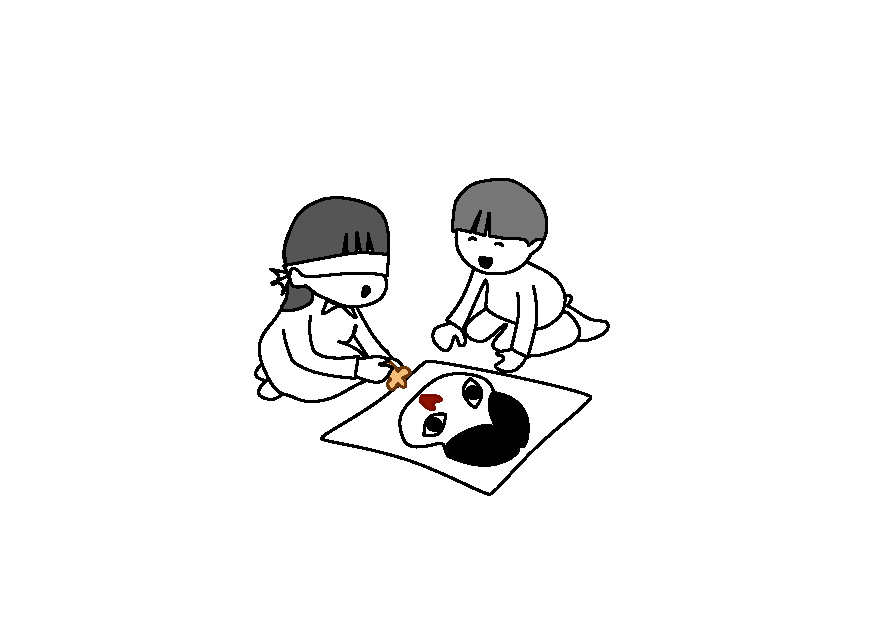
\includegraphics[trim=100 60 100 70, clip, width=.3\hsize]{./img/fukuwarai02.pdf}}
  \caption{Fukuwarai 1/game like ``pin the tail on the donkey.''}
\end{figure}

\subsubsection{Sentences}
\begin{enumerate}
  \ifWB
  \item \ruby{手}{て}ぬぐいで、\underline{\hspace{6em}}して。\mySound{02601}\\Keep a blindfold with a towel.%めかくし%1-26-1-DB
  \else
  \item \ruby{手}{て}ぬぐいで、\underline{\ruby{}{}目隠し}して。\mySound{02601}\\Keep a blindfold with a towel.%めかくし%1-26-1-DB
  \fi%WB
%D4E%ID:1
%D4E%sentence:(手:て)ぬぐいで、<BLANK>して。
%D4E%english:Use a towel as a blindfold.<div><img class=\"qPicture\" src=\"img/fukuwarai01.png\"></div>
%D4E%answer:めかくし
%D4E%model:目隠し
%D4E%roman:mekakushi
%D4E%notes:tenugui (towel); de (with); shite (please do);
  \ifWB
  \item いいですか。これが\ruby{目}{め}、これが\ruby{鼻}{はな}、\underline{\hspace{6em}}よ。\mySound{02602}\\OK? These are eyes. This is a nose. And this is a mouth.%これがくちです%1-26-2-DB
  \else
  \item いいですか。これが\ruby{目}{め}、これが\ruby{鼻}{はな}、\underline{これが\ruby{口}{くち}です}よ。\mySound{02602}\\OK? These are eyes. This is a nose. And this is a mouth.%これがくちです%1-26-2-DB
  \fi%WB
%D4E%ID:2
%D4E%sentence:いいですか。これが(目:め)、これが(鼻:はな)、<BLANK>よ。
%D4E%english:OK? These are the eyes, this is the nose, and this is the mouth.<div><img class=\"qPicture\" src=\"img/fukuwarai01.png\"></div>
%D4E%answer:これがくちです
%D4E%model:これが口です。
%D4E%roman:koregakuchidesu
%D4E%notes:ii (OK); me (eye); hana (nose).
  \ifWB
  \item まず、\ruby{鼻}{はな}を\underline{\hspace{6em}}。\mySound{02603}\\First, put a nose/on the face).%おいて%1-26-3-DB
  \else
  \item まず、\ruby{鼻}{はな}を\underline{\ruby{置}{お}いて}。\mySound{02603}\\First, put a nose/on the face).%おいて%1-26-3-DB
  \fi%WB
%D4E%ID:3
%D4E%sentence:まず、(鼻:はな)を<BLANK>。
%D4E%english:First, put a nose on the face.
%D4E%answer:おいて
%D4E%model:置いて
%D4E%roman:oite
%D4E%notes:mazu (first); hana (nose).
  \ifWB
  \item そうそう、\underline{\hspace{6em}}、\ruby{右}{みぎ}。\mySound{02604}\\All right go on, a bit more, right.%もうすこしみぎ%1-26-4-DB
  \else
  \item そうそう、\underline{もう\ruby{少}{すこ}し}、\ruby{右}{みぎ}。\mySound{02604}\\All right go on, a bit more, right.%もうすこしみぎ%1-26-4-DB
  \fi%WB
%D4E%ID:4
%D4E%sentence:そうそう、<BLANK>、(右:みぎ)。
%D4E%english:All right, go on, a bit more to the right.
%D4E%answer:もうすこし
%D4E%model:もう少し
%D4E%roman:mousukoshi
%D4E%notes:sousou (all right); migi (right).
  \ifWB
  \item もう\ruby{少}{すこ}し、\ruby{左}{ひだり}。\underline{\hspace{6em}}。\mySound{02605}\\A bit more left. More left.%もっとひだり%1-26-5-DB
  \else
  \item もう\ruby{少}{すこ}し、\ruby{左}{ひだり}。\underline{もっと\ruby{左}{ひだり}}。\mySound{02605}\\A bit more to the left. Even more to the left.%もっとひだり%1-26-5-DB
  \fi%WB
%D4E%ID:5
%D4E%sentence:もう(少:すこ)し、(左:ひだり)。<BLANK>。
%D4E%english:A bit more to the left. Even more to the left.
%D4E%answer:もっとひだり
%D4E%model:もっと左
%D4E%roman:mottohidari
%D4E%notes:mou (more); sukoshi (a bit); hidari (left).

  \ifWB
  \item ええ、\underline{\hspace{6em}}、\ruby{上}{うえ}。\mySound{02606}\\Yes, a bit more up.%もうちょっと%1-26-6-DB
  \else
  \item ええ、\underline{もうちょっと}、\ruby{上}{うえ}。\mySound{02606}\\Yes, a bit more up.%もうちょっと%1-26-6-DB
  \fi%WB
%D4E%ID:6
%D4E%sentence:ええ、<BLANK>(上:うえ)。
%D4E%english:Yes, a bit more up.
%D4E%answer:もうちょっと
%D4E%model:もうちょっと
%D4E%roman:mouchotto
%D4E%notes:ue (up).
  \ifWB
  \item で、\underline{\hspace{6em}}、\ruby{下}{した}。\mySound{02607}\\And a bit more down.%もうすこし%1-26-7-DB
  \else
  \item で、\underline{もう\ruby{少}{すこ}し}、\ruby{下}{した}。\mySound{02607}\\And a bit more down.%もうすこし%1-26-7-DB
  \fi%WB
%D4E%ID:7
%D4E%sentence:で、<BLANK>(下:した)。
%D4E%english:And a bit more down.
%D4E%answer:もうすこし
%D4E%model:もう少し
%D4E%roman:mousukoshi
%D4E%notes:de (and); shita (down).
  \ifWB
  \item いや、\underline{\hspace{6em}}\ruby{下}{した}。\mySound{02608}\\No, even further down.%もっともっと%1-26-8-DB
  \else
  \item いや、\underline{もっともっと}\ruby{下}{した}。\mySound{02608}\\No, even further down.%もっともっと%1-26-8-DB

\item いや、\underline{もっともっと}(下:した)。\mySound{02608}\\No, even further down.

  \fi%WB
%D4E%ID:8
%D4E%sentence:いや、<BLANK>(下:した)。
%D4E%english:No, even further down.
%D4E%answer:もっともっと
%D4E%model:もっともっと
%D4E%roman:mottomotto
%D4E%notes:iya (no); shita (down).
  \ifWB
  \item で、ちょっと、\ruby{少}{すこ}し、\underline{\hspace{6em}}。\mySound{02609}\\Just a bit, a tiny bit to the left.%ほんのすこし%1-26-9-DB
  \else
  \item で、ちょっと、\ruby{少}{すこ}し、\underline{ほんの\ruby{少}{すこ}し、\ruby{左}{ひだり}}。\mySound{02609}\\Just a bit, a tiny bit to the left.%ほんのすこし%1-26-9-DB
  \fi%WB
%D4E%ID:9
%D4E%sentence:で、ちょっと、(少:すこ)し、<BLANK>(左:ひだり)。
%D4E%english:Just a bit, a tiny bit to the left.
%D4E%answer:ほんのすこし
%D4E%model:ほんのすこし
%D4E%roman:honnosukoshi
%D4E%notes:de (and); chotto (a bit); sukoshi (a bit); hidari (left).
  \ifWB
  \item はい、よく\underline{\hspace{6em}}。\mySound{02610}\\Yes, you did a great job.%できました%1-26-10-DB
  \else
  \item はい、よく\underline{できました}。\mySound{02610}\\Yes, you did a great job.%できました%1-26-10-DB
  \fi%WB
%D4E%ID:10
%D4E%sentence:はい、よく<BLANK>。
%D4E%english:Yes, you did a great job.
%D4E%answer:できました
%D4E%model:できました
%D4E%roman:dekimashita
%D4E%notes:hai (yes); yoku (well).
\end{enumerate}

\subsubsection{Words and Expressions}
\begin{enumerate}
  \item tenugui/Japanese towel\index{tenugui}/手ぬぐい
  \item de/p.de.with-tool\index{de}/で\label{203740_15Mar19}
  \item mekakushi/blindfold.n.suru.GN\index{mekakushi}/目隠し\label{204027_15Mar19}
  \item me/eye\index{me}/目
  \item mazu/firstly\index{mazu}/まず
  \item hana/nose\index{hana}/鼻
  \item kuchi/mouse\index{kuchi}/口
  \item oite/put.vt.te/置いて\index{oku}
  \item s\=os\=o/all right\index{sousou@s\=os\=o}/そうそう
  \item m\=o-sukoshi/a little more\index{mousukoshi@m\=o-sukoshi}/もう少し
  \item motto/more\index{motto}/もっと
  \item ue/up\index{ue}/上
  \item shita/down\index{shita}/下
  \item honno/little\index{honno}/ほんの
  \item yoku-deki-masita/good job\index{yoku-deki-masita}/よくできました
\end{enumerate}

%\newpage
\ifEnglish
  \subsection{Day 27: Fukuwarai 2}%E
%D4E%day:027
%D4E%title:Fukuwarai 2
\else
  \subsection{Day 27: 福笑い 2}%J
\fi%English

%\subsubsection{Objectives}

Fukuwarai 2/game like ``pin the tail on the donkey''.

\subsubsection{Sentences}
\begin{enumerate}
  \ifWB
  \item \underline{\hspace{6em}}。\mySound{02701}\\Let's move on to the next. it's mouth.%つぎはくち%1-27-1-DB
  \else
  \item \underline{\ruby{次}{つぎ}は\ruby{口}{くち}}。\mySound{02701}\\Let's move on to the next. it's mouth.%つぎはくち%1-27-1-DB
  \fi%WB
%D4E%ID:1
%D4E%sentence:<BLANK>。
%D4E%english:Let's move on to the next. it's mouth.
%D4E%answer:つぎはくち
%D4E%model:次は口
%D4E%roman:tsugihakuchi
%D4E%notes:tsugi (next).
  \ifWB
  \item もっと\ruby{右}{みぎ}、もっと\ruby{右}{みぎ}、\underline{\hspace{6em}}\ruby{右}{みぎ}。\mySound{02702}\\A bit more to the right, a bit more to the right, and a little further right.%もうちょっと%1-27-2-DB
  \else
  \item もっと\ruby{右}{みぎ}、もっと\ruby{右}{みぎ}、\underline{もうちょっと}\ruby{右}{みぎ}。\mySound{02702}\\A bit more to the right, a bit more to the right, and a little further right.%もうちょっと%1-27-2-DB
  \fi%WB
%D4E%ID:2
%D4E%sentence:もっと(右:みぎ)、もっと(右:みぎ)、<BLANK>(右:みぎ)。
%D4E%english:A bit more to the right, a bit more to the right, and a little further right.
%D4E%answer:もうちょっと
%D4E%model:もうちょっと
%D4E%roman:mouchotto
%D4E%notes:motto (more); migi (right).
  \ifWB
  \item そう、で、もうちょっと\ruby{下}{した}。\underline{\hspace{6em}}\ruby{下}{した}。\mySound{02703}\\Good, and a bit more down. A bit more down.%もうちょい%1-27-3-DB
  \else
  \item そう、で、もうちょっと\ruby{下}{した}。\underline{もうちょい}\ruby{下}{した}。\mySound{02703}\\Good, and a bit more down. A bit more down.%もうちょい%1-27-3-DB
  \fi%WB
%D4E%ID:3
%D4E%sentence:そう、で、もうちょっと(下:した)。<BLANK>(下:した)。
%D4E%english:Good, and a bit more down. A bit more down.
%D4E%answer:もうちょい
%D4E%model:もうちょい
%D4E%roman:mouchoi
%D4E%notes:sou (good); de (and); shita (down).
  \ifWB
  \item ああ、\ruby{下過}{したす}ぎた。\underline{\hspace{6em}}。\mySound{02704}\\Oh, no, it passed too go down. Just a little go up.%ほんのすこしうえ%1-27-4-DB
  \else
  \item ああ、\ruby{下過}{したす}ぎた。\underline{ほんの\ruby{少}{すこ}し\ruby{上}{うえ}}。\mySound{02704}\\Oh, no, it passed too go down. Just a little go up.%ほんのすこしうえ%1-27-4-DB
  \fi%WB
%D4E%ID:4
%D4E%sentence:ああ、(下過:したす)ぎた。<BLANK>。
%D4E%english:Oh, no, it passed too go down. Just a little go up.
%D4E%answer:ほんのすこしうえ
%D4E%model:ほんの少し上
%D4E%roman:honnosukoshiue
%D4E%notes:a (oh); shita-sugiru (pass too go down).
  \ifWB
  \item ちょうどいい。\underline{\hspace{6em}}。\mySound{02705}\\It's all right. Exactly.%ぴったり%1-27-5-DB
  \else
  \item ちょうどいい。\underline{ぴったり}。\mySound{02705}\\It's all right. Exactly.%ぴったり%1-27-5-DB
  \fi%WB
%D4E%ID:5
%D4E%sentence:ちょうどいい。<BLANK>。
%D4E%english:It's all right. Exactly.
%D4E%answer:ぴったり
%D4E%model:ぴったり
%D4E%roman:pittari
%D4E%notes:choudo (exactly).

  \ifWB
  \item で、\underline{\hspace{6em}}は\ruby{目}{め}。で、\ruby{右目}{みぎめ}。\mySound{02706}\\And the last one is for eyes. Firstly right eye.%さいごはめ%1-27-6-DB
  \else
  \item で、\underline{\ruby{最後}{さいご}}は\ruby{目}{め}。で、\ruby{右目}{みぎめ}。\mySound{02706}\\And the last one is for eyes. Firstly right eye.%さいごはめ%1-27-6-DB
  \fi%WB
%D4E%ID:6
%D4E%sentence:で、<BLANK>は(目:め)。で、(右目:みぎめ)。
%D4E%english:And the last one is for eyes. Firstly right eye.
%D4E%answer:さいご
%D4E%model:最後
%D4E%roman:saigo
%D4E%notes:de (and); me (eye); migime (right eye).
  \ifWB
  \item \ruby{鼻}{はな}の\ruby{右}{みぎ}、そうそう\underline{\hspace{6em}}。\mySound{02707}\\Put it to the right of the nose. Yes, it's quite simple.%かんたん%1-27-7-DB
  \else
  \item \ruby{鼻}{はな}の\ruby{右}{みぎ}、そうそう\underline{\ruby{簡単}{かんたん}}。\mySound{02707}\\Put it to the right of the nose. Yes, it's quite simple.%かんたん%1-27-7-DB
  \fi%WB
%D4E%ID:7
%D4E%sentence:(鼻:はな)の(右:みぎ)、そうそう<BLANK>。
%D4E%english:Put it to the right of the nose. Yes, it's quite simple.
%D4E%answer:かんたん
%D4E%model:簡単
%D4E%roman:kanntann
%D4E%notes:hana (nose); migi (right).
  \ifWB
  \item で、\ruby{左目}{ひだりめ}、\underline{\hspace{6em}}かな。\mySound{02708}\\And now for the left eye. I think you should move it a bit up.%ちょっとうえ%1-27-8-DB
  \else
  \item で、\ruby{左目}{ひだりめ}、\underline{ちょっと\ruby{上}{うえ}}かな。\mySound{02708}\\And now for the left eye. I think you should move it a bit up.%ちょっとうえ%1-27-8-DB
  \fi%WB
%D4E%ID:8
%D4E%sentence:で、(左目:ひだりめ)、<BLANK>かな。
%D4E%english:And now for the left eye. I think you should move it a bit up.
%D4E%answer:ちょっとうえ
%D4E%model:ちょっと上
%D4E%roman:chottoue
%D4E%notes:hidarime (left eye); ue (up).
  \ifWB
  \item だいたい、いいですね。\underline{\hspace{6em}}ね。\mySound{02709}\\Almost done. You're doing well.%じょうずです%1-27-9-DB
  \else
  \item だいたい、いいですね。\underline{じょうずです}ね。\mySound{02709}\\Almost done. You're doing well.%じょうずです%1-27-9-DB
  \fi%WB
%D4E%ID:9
%D4E%sentence:だいたい、いいですね。<BLANK>ね。
%D4E%english:Almost done. You're doing well.
%D4E%answer:じょうずです
%D4E%model:上手です
%D4E%roman:jouzudesu
%D4E%notes:daitai (almost); ii (good).
  \ifWB
  \item では、\ruby{目隠}{めかく}し、\ruby{外}{はず}して。ほら、\underline{\hspace{6em}}。\mySound{02710}\\Take off your blindfold. Look, it's a funny face.%へんなかお%1-27-10-DB
  \else
  \item では、\ruby{目隠}{めかく}し、\ruby{外}{はず}して。ほら、\underline{\ruby{変}{へん}な\ruby{顔}{かお}}。\mySound{02710}\\Take off your blindfold. Look, it's a funny face.%へんなかお%1-27-10-DB
  \fi%WB
%D4E%ID:10
%D4E%sentence:では、(目隠:めかく)し、(外:はず)して。ほら、<BLANK>。
%D4E%english:Take off your blindfold. Look, it's a funny face.
%D4E%answer:へんなかお
%D4E%model:変な顔
%D4E%roman:hennnakao
%D4E%notes:deha (then); hazushite (remove); hora (look).
\end{enumerate}

\subsubsection{Words and Expressions}
\begin{enumerate}
  \item tsugi/next\index{tsugi}/次
  \item m\=ochoi/little more\index{mouchoi@m\=ochoi}/もうちょい
  \item sita-sugita/passed too\index{sita-sugita}/下過ぎた
  \item ch\=do/just\index{choudo@ch\=do}/ちょうど
  \item pittari/fit\index{pittari}/ぴったり
  \item saigo/last/\index{saigo}/最後
  \item migi-me/right eye\index{migi-me}/右目
  \item hidari-me/left eye\index{hidari-me}/左目
  \item daitai/almost\index{daitai}/だいたい
  \item j\=ozu/good at\index{jouzu@j\=ozu}/じょうず
  \item hazusite/remove.vt.te/外して\index{hazusu}
  \item hora/look\index{hora}/ほら
  \item kao/face\index{kao}/顔
\end{enumerate}

%\newpage
\ifEnglish
  \subsection{Day 28: Try to do something or nothing}%E
%D4E%day:028
%D4E%title:Try to do something or nothing
\else
  \subsection{Day 28: やる気とやる気なし}%J
\fi%English

%\subsubsection{Objectives}

Try to do something or nothing.

\subsubsection{Sentences}
\begin{enumerate}
  \ifWB
  \item \underline{\hspace{6em}}、しよ？\mySound{02801}\\Let's play cards!%トランプ%1-28-1-DB
  \else
  \item \underline{トランプ}、しよ？\mySound{02801}\\Let's play cards!%トランプ%1-28-1-DB
  \fi%WB
%D4E%ID:1
%D4E%sentence:<BLANK>しよ？
%D4E%english:Let's play cards!
%D4E%answer:トランプ
%D4E%model:トランプ
%D4E%roman:(katakana)torannpu(hiragana)
%D4E%notes:shiyo (let's do).
  \ifWB
  \item いやだ！\underline{\hspace{6em}}。\mySound{02802}\\No! I hate losing.%まけるのきらい%1-28-2-DB
  \else
  \item いやだ！\underline{まけるの、\ruby{嫌}{きら}い}。\mySound{02802}\\No! I hate losing.%まけるのきらい%1-28-2-DB
  \fi%WB
%D4E%ID:2
%D4E%sentence:いやだ！<BLANK>。
%D4E%english:No! I hate losing.
%D4E%answer:まけるのきらい
%D4E%model:負けるの嫌い
%D4E%roman:makerunokirai
%D4E%notes:iyada (no I don't like it).
  \ifWB
  \item とにかくやって\underline{\hspace{6em}}よ。\mySound{02803}\\Let's do it anyway.%みましょう%1-28-3-DB
  \else
  \item とにかくやって\underline{みましょう}よ。\mySound{02803}\\Let's do it anyway.%みましょう%1-28-3-DB
  \fi%WB
%D4E%ID:3
%D4E%sentence:とにかくやって<BLANK>よ。
%D4E%english:Let's do it anyway.
%D4E%answer:みましょう
%D4E%model:みましょう
%D4E%roman:mimashou
%D4E%notes:tonikaku (anyway).
  \ifWB
  \item まずは、やってみたら\underline{\hspace{6em}}か。\mySound{02804}\\First, why do not you try it.%どうでしょう%1-28-4-DB
  \else
  \item まずは、やってみたら\underline{どうでしょう}か。\mySound{02804}\\First, why do not you try it.%どうでしょう%1-28-4-DB
  \fi%WB
%D4E%ID:4
%D4E%sentence:まずは、やってみたら<BLANK>か。
%D4E%english:First, why do not you try it.
%D4E%answer:どうでしょう
%D4E%model:どうでしょう
%D4E%roman:doudeshou
%D4E%notes:mazu (first); yatte-mitara (try it).
  \ifWB
  \item パチンコは\underline{\hspace{6em}}。\mySound{02805}\\I often play pachinko.%よくします%1-28-5-DB
  \else
  \item パチンコは\underline{よくします}。\mySound{02805}\\I often play pachinko.%よくします%1-28-5-DB
  \fi%WB
%D4E%ID:5
%D4E%sentence:パチンコは<BLANK>。
%D4E%english:I often play pachinko.
%D4E%answer:よくします
%D4E%model:よくします
%D4E%roman:yokusimasu
%D4E%notes:pachinko (Japanese pinball).

  \ifWB
  \item マージャンも\underline{\hspace{6em}}。\mySound{02806}\\I also do mah-jong sometimes.%ときどきします%1-28-6-DB
  \else
  \item マージャンも\underline{\ruby{時々}{ときどき}します}。\mySound{02806}\\I also do mah-jong sometimes.%ときどきします%1-28-6-DB
  \fi%WB
%D4E%ID:6
%D4E%sentence:マージャンも<BLANK>。
%D4E%english:I also do mah-jong sometimes.
%D4E%answer:ときどきします
%D4E%model:時々します
%D4E%roman:tokidokishimasu
%D4E%notes:mah-jong (mah-jon game).
  \ifWB
  \item けれども、\underline{\hspace{6em}}ですね。\mySound{02807}\\However, I am a kind of social-player.%つきあいていど%1-28-7-DB
  \else
  \item けれども、\underline{\ruby{付}{つ}き\ruby{合}{あ}い\ruby{程度}{ていど}}ですね。\mySound{02807}\\However, I am a kind of social-player.%つきあいていど%1-28-7-DB
  \fi%WB
%D4E%ID:7
%D4E%sentence:けれども、<BLANK>ですね。
%D4E%english:However, I am a kind of social-player (degree of socialization).
%D4E%answer:つきあいていど
%D4E%model:付き合い程度
%D4E%roman:tsukiaiteido
%D4E%notes:keredomo (however).
  \ifWB
  \item \ruby{運動}{うんどう}って、\ruby{ラジオ}{らじお}\underline{\hspace{6em}}ぐらいですね。\mySound{02808}\\Exercise is just only radio exercises.%たいそう%1-28-8-DB
  \else
  \item \ruby{運動}{うんどう}って、\ruby{ラジオ}{らじお}\underline{\ruby{体操}{たいそう}}ぐらいですね。\mySound{02808}\\Exercise is just only radio exercises.%たいそう%1-28-8-DB
  \fi%WB
%D4E%ID:8
%D4E%sentence:(運動:うんどう)って、(ラジオ:らじお)<BLANK>ぐらいですね。
%D4E%english:Exercise is just only radio exercises.
%D4E%answer:たいそう
%D4E%model:体操
%D4E%roman:taisou
%D4E%notes:undou (exercise); rajio (radio).
  \ifWB
  \item \underline{\hspace{6em}}はしませんね、ほとんど。\mySound{02809}\\I seldom exercise, and I almost don't do anything that could be considered real exercise.%うんどうらしいうんどう%1-28-9-DB
  \else
  \item \underline{\ruby{運動}{うんどう}らしい\ruby{運動}{うんどう}}はしませんね、ほとんど。\mySound{02809}\\I seldom exercise, and I almost don't do anything that could be considered real exercise.%うんどうらしいうんどう%1-28-9-DB
  \fi%WB
%D4E%ID:9
%D4E%sentence:<BLANK>はしませんね、ほとんど。
%D4E%english:I seldom exercise, and I almost don't do anything that could be considered real exercise.
%D4E%answer:うんどうらしいうんどう
%D4E%model:運動らしい運動
%D4E%roman:unndourashiiunndou
%D4E%notes:hotondo (seldomly).
  \ifWB
  \item \ruby{マラソン}{まらそん}？\underline{\hspace{6em}}よ。\mySound{02810}\\Marathon? I would die.%しんでしまいます%1-28-10-DB
  \else
  \item \ruby{マラソン}{まらそん}？\underline{\ruby{死}{し}んでしまいます}よ。\mySound{02810}\\Marathon? I would die.%しんでしまいます%1-28-10-DB
  \fi%WB
%D4E%ID:10
%D4E%sentence:(マラソン:まらそん)？<BLANK>よ。
%D4E%english:Marathon? I would die.
%D4E%answer:しんでしまいます
%D4E%model:死んでしまいます
%D4E%roman:shindeshimaimasu
%D4E%notes:marason (marathon).
\end{enumerate}


\subsubsection{Words and Expressions}
\begin{enumerate}
  \item toranpu/card games\index{toranpu}/トランプ
  \item shiyo/do.v.vol.GN\index{shiyo}/しよ\label{215602_15Mar19}
  \item iya/hate.na-adj/いや\index{iya}
  \item kirai/dislike.na-adj/嫌い\index{kirai}
  \item tonikaku/anyway\index{tonikaku}/とにかく
  \item --tara-d\=o-desh\=oka/how about..ing?\index{taradoudeshouka@--tara-d\=o-desh\=oka}/--たらどうでしょうか
  \item pachinko/pachinko\index{pachinko}/パチンコ
  \item m\=ajan/mah-jong\index{maajan@m\=ajan}/マージャン
  \item tokidoki/from time to time\index{tokidoki}/時々
  \item keredomo/but\index{keredomo}/けれども
  \item tsukiai/keep-company.vi.masu/付き合い\index{tsukiau}
  \item tsukiau/keep-company.vi/付き合う\index{tsukiau}
  \item teido/degree\index{teido}/程度
  \item und\=o/exercises\index{undou@und\=o}/運動
  \item rajio/radio\index{rajio}/ラジオ
  \item tais\=o/exercises\index{taisou@tais\=o}/体操
  \item --rashii/like..\index{rashii@--rashii}/--らしい
  \item hotondo/seldomly\index{hotondo}/ほとんど
  \item marason/marathon\index{marason}/マラソン
  \item shinde/die.vi.te/死んで\index{shinu}
  \item --teshimau/aux.complete.GN\index{teshimau@--teshimau}/--しまう\label{223150_25Feb20}
\end{enumerate}

%\newpage
\ifEnglish
  \section{Week 5: Interaction and Strategies}
\else
  \section{Week 5: インタラクションとストラテジ}
\fi%English

\ifEnglish
  When you do not understand what the other person says, there is no need to bother to bother.
\else
  相手の言っていることがわからないとき、わざわざわからないという必要はありません。
\fi
\ifEnglish
  It might be nice to have a nice smile for a while.
\else
  少々笑顔を見せて、しばらく頷いているのもいいでしょう。
\fi

%\newpage
\ifEnglish
  \subsection{Day 29: Regret}%E
%D4E%day:029
%D4E%title:Regret
\else
  \subsection{Day 29: 後悔する}%J
\fi%English

%\subsubsection{Objectives}

\ifEnglish
  ``k\=okai sakini tatazu'' (It's no use crying over spilt milk; lit. regret is not the first to go),
  which means that no matter how much you regret what has already been done, you can't get it back later.
\else
  「後悔先に立たず」とは、すでに終わったことを、いくら後で悔やんでも取り返しがつかないということ。
\fi%English

\subsubsection{Sentences}
\begin{enumerate}
  \ifWB
  \item ああ、\underline{\hspace{6em}}。\mySound{02901}\\Oh, sorry.%ざんねん%1-29-1-DB
  \else
  \item ああ、\underline{\ruby{残念}{ざんねん}}。\mySound{02901}\\Oh, sorry.%ざんねん%1-29-1-DB
  \fi%WB
%D4E%ID:1
%D4E%sentence:ああ、<BLANK>。
%D4E%english:Oh, sorry.
%D4E%answer:ざんねん
%D4E%model:残念
%D4E%roman:zannnenn
%D4E%notes:aa (oh).
  \ifWB
  \item \underline{\hspace{6em}}ね。\mySound{02902}\\I am sorry. It was not good.%ざんねんでした%1-29-2-DB
  \else
  \item \underline{\ruby{残念}{ざんねん}でした}ね。\mySound{02902}\\I am sorry. It was not good.%ざんねんでした%1-29-2-DB
  \fi%WB
%D4E%ID:2
%D4E%sentence:<BLANK>ね。
%D4E%english:I am sorry. It was not good.
%D4E%answer:ざんねんでした
%D4E%model:残念でした
%D4E%roman:zannnenndeshita
%D4E%notes:ne (isn't it).
  \ifWB
  \item ..というのは？..\underline{\hspace{6em}}でしょうか？\mySound{02903}\\And? What do you mean?%どういうこと%1-29-3-DB
  \else
  \item ..というのは？..\underline{どういうこと}でしょうか？\mySound{02903}\\And? What do you mean?%どういうこと%1-29-3-DB
  \fi%WB
%D4E%ID:3
%D4E%sentence:..というのは？..<BLANK>でしょうか？
%D4E%english:And? What do you mean?
%D4E%answer:どういうこと
%D4E%model:どういうこと
%D4E%roman:douiukoto
%D4E%notes:
  \ifWB
  \item \ruby{変}{へん}なこというから、\underline{\hspace{6em}}よ。\mySound{02904}\\You said something strange, and now I've lost my motivation.%やるきうせた%1-29-4-DB
  \else
  \item \ruby{変}{へん}なこというから、\underline{やる\ruby{気}{き}、\ruby{失}{う}せた}よ。\mySound{02904}\\You said something strange, and now I've lost my motivation.%やるきうせた%1-29-4-DB
  \fi%WB
%D4E%ID:4
%D4E%sentence:(変:へん)なこというから、<BLANK>よ。
%D4E%english:You said something strange, and now I've lost my motivation.
%D4E%answer:やるきうせた
%D4E%model:やる気失せた
%D4E%roman:yarukiuseta
%D4E%notes:hennna (strange).
  \ifWB
  \item そうだそうだ、\ruby{謝}{あやま}るなら\underline{\hspace{6em}}だ。\mySound{02905}\\Yes, that's right! If you're going to apologize, now's your chance.%いまのうち%1-29-5-DB
  \else
  \item そうだそうだ、\ruby{謝}{あやま}るなら\underline{\ruby{今}{いま}のうち}だ。\mySound{02905}\\Yes, that's right! If you're going to apologize, now's your chance.%いまのうち%1-29-5-DB
  \fi%WB
%D4E%ID:5
%D4E%sentence:そうだそうだ、(謝:あやま)るなら<BLANK>だ。
%D4E%english:Yes, that's right! If you're going to apologize, now's your chance.
%D4E%answer:いまのうち
%D4E%model:今のうち
%D4E%roman:imanouchi
%D4E%notes:

  \ifWB
  \item いや、それは\underline{\hspace{6em}}ですね。\mySound{02906}\\Really! I'm sorry to hear that.%それはおきのどく%1-29-6-DB
  \else
  \item いや、それは\underline{お\ruby{気}{き}の\ruby{毒}{どく}}ですね。\mySound{02906}\\Really! I'm sorry to hear that.%それはおきのどく%1-29-6-DB
  \fi%WB
%D4E%ID:6
%D4E%sentence:いや、それは<BLANK>ですね。
%D4E%english:Really! I'm sorry to hear that.
%D4E%answer:おきのどく
%D4E%model:お気の毒
%D4E%roman:okinodoku
%D4E%notes:sore ha (that).
  \ifWB
  \item ずいぶん\underline{\hspace{6em}}をしましたよ。\mySound{02907}\\I had terrible feelings a lot.%くやしいおもい%1-29-7-DB
  \else
  \item ずいぶん\underline{\ruby{悔}{くや}しい\ruby{思}{おも}い}をしましたよ。\mySound{02907}\\I had terrible feelings a lot.%くやしいおもい%1-29-7-DB
  \fi%WB
%D4E%ID:7
%D4E%sentence:ずいぶん<BLANK>をしましたよ。
%D4E%english:I had terrible feelings a lot.
%D4E%answer:くやしいおもい
%D4E%model:悔しい思い
%D4E%roman:kuyashiiomoi
%D4E%notes:zuibun (a lot).
  \ifWB
  \item \ruby{途中}{とちゅう}でやめるのは、なんだか\underline{\hspace{6em}}です。\mySound{02908}\\It is somewhat regrettable to stop it halfway.%なんだかこころのこり%1-29-8-DB
  \else
  \item \ruby{途中}{とちゅう}でやめるのは、なんだか\underline{\ruby{心残}{こころのこ}り}です。\mySound{02908}\\It is somewhat regrettable to stop it halfway.%なんだかこころのこり%1-29-8-DB
  \fi%WB
%D4E%ID:8
%D4E%sentence:(途中:とちゅう)でやめるのは、なんだか<BLANK>です。
%D4E%english:It is somewhat regrettable to stop it halfway.
%D4E%answer:こころのこり
%D4E%model:心残り
%D4E%roman:kokoronokori
%D4E%notes:tochuu (halfway); yameru (stop); nanndaka (somewhat).
  \ifWB
  \item \underline{\hspace{6em}}をしたなと\ruby{思}{おも}います。\mySound{02909}\\I think I did something poor for her.%かわいそうなこと%1-29-9-DB
  \else
  \item \underline{かわいそうなこと}をしたなと\ruby{思}{おも}います。\mySound{02909}\\I think I did something poor for her.%かわいそうなこと%1-29-9-DB
  \fi%WB
%D4E%ID:9
%D4E%sentence:<BLANK>をしたなと(思:おも)います。
%D4E%english:I think I did something poor for her.
%D4E%answer:かわいそうなこと
%D4E%model:かわいそうなこと
%D4E%roman:kawaisounakoto
%D4E%notes:omoimasu (think).
  \ifWB
  \item \underline{\hspace{6em}}よね。\ruby{試合}{しあい}に\ruby{負}{ま}けちゃったから。\mySound{02910}\\Yeah, it's disappointing, isn't it? Since you lost the game.%くやしいです%1-29-10-DB
  \else
  \item \underline{\ruby{悔}{くや}しいです}よね。\ruby{試合}{しあい}に\ruby{負}{ま}けちゃったから。\mySound{02910}\\Yeah, it's disappointing, isn't it? Since you lost the game.%くやしいです%1-29-10-DB
  \fi%WB
%D4E%ID:10
%D4E%sentence:<BLANK>よね。(試合:しあい)に(負:ま)けちゃったから。
%D4E%english:Yeah, it's disappointing, isn't it? Since you lost the game.
%D4E%answer:くやしいです
%D4E%model:悔しいです
%D4E%roman:kuyashiidesu
%D4E%notes:shiai (game); makechatta (lost).
\end{enumerate}

\subsubsection{Words and Expressions}
\begin{enumerate}
  \item zannen/sorry.na-adj/残念\index{zannen}
  \item ..to-iu-no-wa/which is?/..というのは\index{toiunowa@..to-iu-no-wa}
  \item d\=o-iu-koto-desh\=oka/what do you mean/どういうことでしょうか\index{douiukoto@d\=o-iu-koto-desh\=oka}
  \item henna-koto/strange thing/変なこと\index{henna-koto}
  \item yaruki/motivation/やる気\index{yaruki}
  \item useta/dissapear.vi.ta/失せた\index{useru}
  \item ayamaru/approgize.vi/謝る\index{ayamaru}
  \item --nara/if you do/--なら\index{nara@--nara}
  \item ima/now/今\index{ima}
  \item uchi/within/うち\index{uchi}
  \item oki-no-doku/sorry,bad/お気の毒\index{oki-no-doku}
  \item kuyashii/regret/悔しい\index{kuyashii}
  \item omoi/feeling.n.masu/思い\index{omoi}
  \item toch\=u/halfway/途中\index{toch\=u}
  \item nandaka/somewhat/なんだか\index{nandaka}
  \item kokoro-nokori/regrettable/心残り\index{kokoro-nokori}
  \item kawaisouna/poor.na-adj/かわいそうな\index{kawaisouna}
  \item omoimasu/think.vt.formal/思います\index{omou}
  \item shiai/game/試合\index{shiai}
  \item make/lose.vi/負け\index{makeru}
  \item --chatta/aux.complete.past.GN/--ちゃった\index{chatta@--chatta}\label{222019_15Mar19}
\end{enumerate}

%\newpage
\ifEnglish
  \subsection{Day 30: Appreciation}%E
%D4E%day:030
%D4E%title:Appreciation
\else
  \subsection{Day 30: 賞賛する}%J
\fi%English

%\subsubsection{Objectives}

Praise

\subsubsection{Sentences}
\begin{enumerate}
  \ifWB
  \item \underline{\hspace{6em}}ですね。\mySound{03001}\\It is wonderful.%すばらしい%1-30-1-DB
  \else
  \item \underline{すばらしい}ですね。\mySound{03001}\\It is wonderful.%すばらしい%1-30-1-DB
  \fi%WB
%D4E%ID:1
%D4E%sentence:<BLANK>ですね。
%D4E%english:It is wonderful.
%D4E%answer:すばらしい
%D4E%model:すばらしい
%D4E%roman:subarashii
%D4E%notes:
  \ifWB
  \item \underline{\hspace{6em}}ですね。\mySound{03002}\\It is quite nice.%なかなかいい%1-30-2-DB
  \else
  \item \underline{なかなかいい}ですね。\mySound{03002}\\It is quite nice.%なかなかいい%1-30-2-DB
  \fi%WB
%D4E%ID:2
%D4E%sentence:<BLANK>ですね。
%D4E%english:It is quite nice.
%D4E%answer:なかなかいい
%D4E%model:なかなかいい
%D4E%roman:nakanakaii
%D4E%notes:
  \ifWB
  \item \underline{\hspace{6em}}にできました。\mySound{03003}\\You made it very well.%じょうず%1-30-3-DB
  \else
  \item \underline{じょうず}にできました。\mySound{03003}\\You made it very well.%じょうず%1-30-3-DB
  \fi%WB
%D4E%ID:3
%D4E%sentence:<BLANK>にできました。
%D4E%english:You made it very well.
%D4E%answer:じょうず
%D4E%model:上手に
%D4E%roman:jouzuni
%D4E%notes:dekimashita (made it).
  \ifWB
  \item だんだん\underline{\hspace{6em}}きましたね。\mySound{03004}\\You gradually improved, didn't you?%じょうたつして%1-30-4-DB
  \else
  \item だんだん\underline{\ruby{上達}{じょうたつ}して}きましたね。\mySound{03004}\\You gradually improved, didn't you?%じょうたつして%1-30-4-DB
  \fi%WB
%D4E%ID:4
%D4E%sentence:だんだん<BLANK>きましたね。
%D4E%english:You gradually improved, didn't you?
%D4E%answer:じょうたつして
%D4E%model:上達して
%D4E%roman:joutatsushite
%D4E%notes:danndann (gradually); kimashita (came).
  \ifWB
  \item \underline{\hspace{6em}}\ruby{色}{いろ}ですね。\mySound{03005}\\It is a brilliant color, isn't it?%あざやかな%1-30-5-DB
  \else
  \item \underline{\ruby{鮮}{あざ}やかな}\ruby{色}{いろ}ですね。\mySound{03005}\\It is a brilliant color, isn't it?%あざやかな%1-30-5-DB
  \fi%WB
%D4E%ID:5
%D4E%sentence:<BLANK>(色:いろ)ですね。
%D4E%english:It is a brilliant color, isn't it?
%D4E%answer:あざやかな
%D4E%model:鮮やかな
%D4E%roman:azayakana
%D4E%notes:iro (color).

  \ifWB
  \item \ruby{明}{あか}るい\underline{\hspace{6em}}ね。\mySound{03006}\\It feels bright.%かんじがします%1-30-6-DB
  \else
  \item \ruby{明}{あか}るい\underline{\ruby{感}{かん}じがします}ね。\mySound{03006}\\It feels bright.%かんじがします%1-30-6-DB
  \fi%WB
%D4E%ID:6
%D4E%sentence:(明:あか)るい<BLANK>ね。
%D4E%english:It feels bright.
%D4E%answer:かんじがします
%D4E%model:感じがします
%D4E%roman:kannjigashimasu
%D4E%notes:akarui (bright).
  \ifWB
  \item なんか\underline{\hspace{6em}}ですね。\mySound{03007}\\It is a nice feeling.%いいかんじ%1-30-7-DB
  \else
  \item なんか\underline{いい\ruby{感}{かん}じ}ですね。\mySound{03007}\\It is a nice feeling.%いいかんじ%1-30-7-DB
  \fi%WB
%D4E%ID:7
%D4E%sentence:なんか<BLANK>ですね。
%D4E%english:It is a nice feeling.
%D4E%answer:いいかんじ
%D4E%model:いい感じ
%D4E%roman:iikannji
%D4E%notes:nanka (somewhat).
  \ifWB
  \item \underline{\hspace{6em}}ね。\mySound{03008}\\That is wonderful.%さすがです%1-30-8-DB
  \else
  \item \underline{さすがです}ね。\mySound{03008}\\That is wonderful.%さすがです%1-30-8-DB
  \fi%WB
%D4E%ID:8
%D4E%sentence:<BLANK>ね。
%D4E%english:That is wonderful.
%D4E%answer:さすがです
%D4E%model:さすがです
%D4E%roman:sasugadesu
%D4E%notes:
  \ifWB
  \item \underline{\hspace{6em}}、ありますよね。\mySound{03009}\\You have good taste.%せんす%1-30-9-DB
  \else
  \item \underline{センス}、ありますよね。\mySound{03009}\\You have good taste.%せんす%1-30-9-DB
  \fi%WB
%D4E%ID:9
%D4E%sentence:<BLANK>、ありますよね。
%D4E%english:You have good taste.
%D4E%answer:センス
%D4E%model:センス
%D4E%roman:(katakana)sennsu(hiragana)
%D4E%notes:arimasu (have).
  \ifWB
  \item \underline{\hspace{6em}}になります。\mySound{03010}\\I have learned a lot.%べんきょう%1-30-10-DB
  \else
  \item \underline{\ruby{勉強}{べんきょう}}になります。\mySound{03010}\\I have learned a lot.%べんきょう%1-30-10-DB
  \fi%WB
%D4E%ID:10
%D4E%sentence:<BLANK>になります。
%D4E%english:I have learned a lot.
%D4E%answer:べんきょう
%D4E%model:勉強
%D4E%roman:bennkyou
%D4E%notes:..ni narimasu (be informative).
\end{enumerate}

\subsubsection{Words and Expressions}
\begin{enumerate}
  \item subarashii/wonderful.i-adj/すばらしい\index{subarashii}
  \item nakanaka/quite\index{nakanaka}/なかなか
  \item j\=ozu-ni/very well\index{jouzuni@j\=ozu-ni}/じょうずに\label{222216_15Mar19}
  \item dandan/gradually\index{dandan}/だんだん
  \item j\=otatsu/improve.n.suru\index{joutatsu@j\=otatsu}/上達
  \item --tekimashita/$\rightarrow$--tekuru/--てきました
  \item --tekuru/GN.aux.become\index{tekuru@--tekuru}/--てくる\label{222400_15Mar19}
  \item azayakana/briliant.na-adj/鮮やかな\index{azayaka}
  \item iro/color\index{iro}/色
  \item akarui/bright.i-adj/明るい\index{akarui}
  \item nanka/somewhat\index{nanka}/なんか
  \item ii-kanji/nice feeling\index{ii-kanji}/いい感じ
  \item sasuga/as expected\index{sasuga}/さすが
  \item sensu/taste\index{sensu}/センス
  \item benky\=o/study.n.suru\index{benky\=o}/勉強
  \item benky\=o-ni-naru/be informative\index{benky\=o-ni-naru}/勉強になる
\end{enumerate}

%\newpage
\ifEnglish
  \subsection{Day 31: Suggestion}%E
%D4E%day:031
%D4E%title:Suggestion
\else
  \subsection{Day 31: 提案する}%J
\fi%English

%\subsubsection{Objectives}

Suggestion

\subsubsection{Sentences}
\begin{enumerate}
  \ifWB
  \item とにかく\underline{\hspace{6em}}というのもひとつの\ruby{方法}{ほうほう}です。\mySound{03101}\\It is one way to try it anyway.%やってみる%1-31-1-DB
  \else
  \item とにかく\underline{やってみる}というのもひとつの\ruby{方法}{ほうほう}です。\mySound{03101}\\It is one way to try it anyway.%やってみる%1-31-1-DB
  \fi%WB
%D4E%ID:1
%D4E%sentence:とにかく<BLANK>というのもひとつの(方法:ほうほう)です。
%D4E%english:It is one way to try it anyway.
%D4E%answer:やってみる
%D4E%model:やってみる
%D4E%roman:yattemiru
%D4E%notes:tonikaku (anyway); houhou (method).
  \ifWB
  \item ひとつひとつ\underline{\hspace{6em}}のもいいですね。\mySound{03102}\\It is good to try to do one by one.%かたづける%1-31-2-DB
  \else
  \item ひとつひとつ\underline{\ruby{片付}{かたづ}ける}のもいいですね。\mySound{03102}\\It is good to try to do one by one.%かたづける%1-31-2-DB
  \fi%WB
%D4E%ID:2
%D4E%sentence:ひとつひとつ<BLANK>のもいいですね。
%D4E%english:It is good to try to do one by one.
%D4E%answer:かたづける
%D4E%model:片付ける
%D4E%roman:katadukeru
%D4E%notes:hitotsu (one).
  \ifWB
  \item \ruby{抽象的}{ちゅうしょうてき}な\underline{\hspace{6em}}もわるくありませんが、..。\mySound{03103}\\Although abstract explanation is not bad...%せつめい%1-31-3-DB
  \else
  \item \ruby{抽象的}{ちゅうしょうてき}な\underline{\ruby{説明}{せつめい}}もわるくありませんが、..。\mySound{03103}\\Although abstract explanation is not bad...%せつめい%1-31-3-DB
  \fi%WB
%D4E%ID:3
%D4E%sentence:(抽象的:ちゅうしょうてき)な<BLANK>もわるくありませんが、..。
%D4E%english:Although abstract explanation is not bad...
%D4E%answer:せつめい
%D4E%model:説明
%D4E%roman:setsumei
%D4E%notes:chyuushouteki (abstract); warukuarimasen (not bad).
  \ifWB
  \item \underline{\hspace{6em}}な\ruby{例}{れい}も\ruby{効果的}{こうかてき}です。\mySound{03104}\\Concrete examples are also effective.%ぐたいてきな%1-31-4-DB
  \else
  \item \underline{\ruby{具体的}{ぐたいてきな}}な\ruby{例}{れい}も\ruby{効果的}{こうかてき}です。\mySound{03104}\\Concrete examples are also effective.%ぐたいてきな%1-31-4-DB
  \fi%WB
%D4E%ID:4
%D4E%sentence:<BLANK>な(例:れい)も(効果的:こうかてき)です。
%D4E%english:Concrete examples are also effective.
%D4E%answer:ぐたいてき
%D4E%model:具体的
%D4E%roman:gutaiteki
%D4E%notes:rei (example); koukateki (effective).
  \ifWB
  \item \underline{\hspace{6em}}\ruby{イメージ}{いめーじ}がありますか？\mySound{03105}\\What kind of image do you have?%どんな%1-31-5-DB
  \else
  \item \underline{どんな}\ruby{イメージ}{いめーじ}がありますか？\mySound{03105}\\What kind of image do you have?%どんな%1-31-5-DB
  \fi%WB
%D4E%ID:5
%D4E%sentence:<BLANK>(イメージ:いめーじ)がありますか？
%D4E%english:What kind of image do you have?
%D4E%answer:どんな
%D4E%model:どんな
%D4E%roman:donnna
%D4E%notes:imeeji (image).

  \ifWB
  \item \underline{\hspace{6em}}なものでも\ruby{構}{かま}いませんよ。\mySound{03106}\\An intuitive idea is fine too.%ちょっかんてき%1-31-6-DB
  \else
  \item \underline{\ruby{直感的}{ちょっかんてき}}なものでも\ruby{構}{かま}いませんよ。\mySound{03106}\\An intuitive idea is fine too.%ちょっかんてき%1-31-6-DB
  \fi%WB
%D4E%ID:6
%D4E%sentence:<BLANK>なものでも(構:かま)いませんよ。
%D4E%english:An intuitive idea is fine too.
%D4E%answer:ちょっかんてき
%D4E%model:直感的
%D4E%roman:chokkannteki
%D4E%notes:kamaimasen (OK).
  \ifWB
  \item \underline{\hspace{6em}}ではどんなものがありますか？\mySound{03107}\\What familiar things do you have around you?%みじかなもの%1-31-7-DB
  \else
  \item \underline{\ruby{身近}{みじか}なもの}ではどんなものがありますか？\mySound{03107}\\What familiar things do you have around you?%みじかなもの%1-31-7-DB
  \fi%WB
%D4E%ID:7
%D4E%sentence:<BLANK>ではどんなものがありますか？
%D4E%english:What familiar things do you have around you?
%D4E%answer:みじかなもの
%D4E%model:身近なもの
%D4E%roman:mijikanamono
%D4E%notes:donnna (what kind); arimasuka (are there).
  \ifWB
  \item なるほど、ではもう\ruby{少}{すこ}し、\ruby{具体的}{ぐたいてき}に\underline{\hspace{6em}}してみましょうよ。\mySound{03108}\\I see. Let’s try to express it a bit more concretely.%ひょうげんして%1-31-8-DB
  \else
  \item なるほど、ではもう\ruby{少}{すこ}し、\ruby{具体的}{ぐたいてき}に\underline{\ruby{表現}{ひょうげん}}してみましょうよ。\mySound{03108}\\I see. Let’s try to express it a bit more concretely.%ひょうげんして%1-31-8-DB
  \fi%WB
%D4E%ID:8
%D4E%sentence:なるほど、ではもう(少:すこ)し、(具体的:ぐたいてき)に<BLANK>してみましょうよ。
%D4E%english:I see. Let’s try to express it a bit more concretely.
%D4E%answer:ひょうげん
%D4E%model:表現
%D4E%roman:hyougenn
%D4E%notes:naruhodo (I see); sukoshi (a bit); mousukoshi (a bit more).
  \ifWB
  \item なにか\underline{\hspace{6em}}があるといいですね。\mySound{03109}\\It would be helpful to have some good examples.%いいれい%1-31-9-DB
  \else
  \item なにか\underline{\ruby{何}{なに}かいい\ruby{例}{れい}}があるといいですね。\mySound{03109}\\It would be helpful to have some good examples.%いいれい%1-31-9-DB
  \fi%WB
%D4E%ID:9
%D4E%sentence:なにか<BLANK>があるといいですね。
%D4E%english:It would be helpful to have some good examples.
%D4E%answer:いいれい
%D4E%model:いい例
%D4E%roman:iirei
%D4E%notes:nanika (something); ii (good).
  \ifWB
  \item いっしょに\underline{\hspace{6em}}か？\mySound{03110}\\How about we think about it together?%かんがえません%1-31-10-DB
  \else
  \item いっしょに\underline{\ruby{考}{かんが}えません}か？\mySound{03110}\\How about we think about it together?%かんがえません%1-31-10-DB
  \fi%WB
%D4E%ID:10
%D4E%sentence:いっしょに<BLANK>か？
%D4E%english:How about we think about it together?
%D4E%answer:かんがえません
%D4E%model:考えません
%D4E%roman:kanngaemasenn
%D4E%notes:isshoni (together).
\end{enumerate}

\subsubsection{Words and Expressions}
\begin{enumerate}
  \item h\=oh\=o/method/way\index{houhou@h\=oh\=o/method}/方法
  \item katazukeru/put-away.vt\index{katazukeru}/片付ける
  \item ch\=ush\=o-teki-na/abstract.na-adj/抽象的な\index{chushoteki@ch\=ush\=o-teki}
  \item setsumei/explanation.n.suru\index{setsumei}/説明
  \item gutai-teki-na/concrete.na-adj/具体的な\index{gutaiteki}
  \item rei/example\index{rei}/例
  \item k\=oka-teki/effective.na-adj/効果的\index{kokateki@\=oka-teki}
  \item im\=eji/image\index{imeji@im\=eji}/イメージ
  \item chokkantekina/intuitive.na-adj/直感的な\index{chokkanteki}
  \item kamaimasen/do not care\index{kamaimasen}/構いません
  \item mijikana/be-familiar.na-adj/身近な\index{mijika}
  \item naruhodo/I see\index{naruhodo}/なるほど
  \item hy\=ogen/express.n.suru\index{hyogen@hy\=ogen}/表現
  \item kangae/think.n-masu\index{kangae}/考え
  \item kangaeru/think.vt\index{kangaeru}/考える
  \item --masenka/how about.GN\index{masenka@--masenka}/--ませんか\label{115732_16Mar19}
\end{enumerate}

%\newpage
\ifEnglish
  \subsection{Day 32: Experience}%E
%D4E%day:032
%D4E%title:Experience
\else
  \subsection{Day 32: 経験がある}%J
\fi%English

\begin{comment}
  経験を述べて、できることを示す。
\end{comment}

%\subsubsection{Objectives}

Experience can be stated and demonstrated

\subsubsection{Sentences}
\label{120351_16Mar19}
\begin{enumerate}
  \ifWB
  \item \ruby{以前}{いぜん}、やったことがあるので、たぶん\underline{\hspace{6em}}だと\ruby{思}{おも}います。\mySound{03201}\\Since I've done it before, I think it should be fine.%だいじょうぶ%1-32-1-DB
  \else
  \item \ruby{以前}{いぜん}、やったことがあるので、たぶん\underline{\ruby{大丈夫}{だいじょうぶ}}だと\ruby{思}{おも}います。\mySound{03201}\\Since I've done it before, I think it should be fine.%だいじょうぶ%1-32-1-DB
  \fi%WB
%D4E%ID:1
%D4E%sentence:(以前:いぜん)、やったことがあるので、たぶん<BLANK>だと(思:おも)います。
%D4E%english:Because I have done it before, I think that it is probably okay.
%D4E%answer:だいじょうぶ
%D4E%model:大丈夫
%D4E%roman:daijoubu
%D4E%notes:izenn (before); tabun (may be); omou (think)
  \ifWB
  \item \ruby{前}{まえ}に\underline{\hspace{6em}}。できると\ruby{思}{おも}います。\mySound{03202}\\Yes, I've done it before, so I think I can do it.%やったことあります%1-32-2-DB
  \else
  \item \ruby{前}{まえ}に\underline{やったことあります}。できると\ruby{思}{おも}います。\mySound{03202}\\Yes, I've done it before, so I think I can do it.%やったことあります%1-32-2-DB
  \fi%WB
%D4E%ID:2
%D4E%sentence:(前:まえ)に<BLANK>。できると(思:おも)います。
%D4E%english:Yes, I've done it before, so I think I can do it.
%D4E%answer:やったことあります
%D4E%model:やったことあります
%D4E%roman:yattakotoarimasu
%D4E%notes:maeni (before); dekiru (can do); omoimasu (think).
  \ifWB

  \item まったくはじめてなんで\underline{\hspace{6em}}。\mySound{03203}\\Since it’s my first time, I’m not sure if I’ll be able to do it.%できるかどうか%1-32-3-DB
  \else
  \item まったくはじめてなんで\underline{はじめてなんでできるかどうか}。\mySound{03203}\\Since it’s my first time, I’m not sure if I’ll be able to do it.%できるかどうか%1-32-3-DB
  \fi%WB
%D4E%ID:3
%D4E%sentence:まったくはじめてなんで<BLANK>。
%D4E%english:I don't know whether I can do it or not since it's for the first time.
%D4E%answer:できるかどうか
%D4E%model:できるかどうか
%D4E%roman:dekirukadouka
%D4E%notes:mattaku (completely); hajimete (for the first time).
  \ifWB
  \item やったこと\underline{\hspace{6em}}よ。でもおもしろそうですよね。\mySound{03204}\\I've never done it, but it looks interesting, doesn't it?%ないんです%1-32-4-DB
  \else
  \item やったこと\underline{ないんです}よ。でもおもしろそうですよね。\mySound{03204}\\I've never done it, but it looks interesting, doesn't it?%ないんです%1-32-4-DB
  \fi%WB
%D4E%ID:4
%D4E%sentence:やったこと<BLANK>よ。でもおもしろそうですよね。
%D4E%english:I've never done it, but it looks interesting, doesn't it?
%D4E%answer:ないんです
%D4E%model:ないんです
%D4E%roman:nainndesu
%D4E%notes:omoshirosou (looks interesting)
  \ifWB
  \item \ruby{確}{たし}かに、やったことは\underline{\hspace{6em}}が、よく\ruby{覚}{おぼ}えていなくて。\mySound{03205}\\I'm sure I've done it before, but I don't remember it clearly.%あるんです%1-32-5-DB
  \else
  \item \ruby{確}{たし}かに、やったことは\underline{あるんです}が、よく\ruby{覚}{おぼ}えていなくて。\mySound{03205}\\I'm sure I've done it before, but I don't remember it clearly.%あるんです%1-32-5-DB
  \fi%WB
%D4E%ID:5
%D4E%sentence:(確:たし)かに、やったことは<BLANK>が、よく(覚:おぼ)えていなくて。
%D4E%english:I'm sure I've done it before, but I don't remember it clearly.
%D4E%answer:あるんです
%D4E%model:あるんです
%D4E%roman:arunndesu
%D4E%notes:tashikani (surely); yattakoto (have done); yoku (well); oboeru (remember).

  \ifWB
  \item \ruby{経験}{けいけん}だけがあるだけで、\underline{\hspace{6em}}とはいえないんですね。\mySound{03206}\\I only have a bit of experience, so I wouldn't say I'm very good at it.%あまりうまい%1-32-6-DB
  \else
  \item \ruby{経験}{けいけん}だけがあるだけで、\underline{あまりうまい}とはいえないんですね。\mySound{03206}\\I only have a bit of experience, so I wouldn't say I'm very good at it.%あまりうまい%1-32-6-DB
  \fi%WB
%D4E%ID:6
%D4E%sentence:(経験:けいけん)だけがあるだけで、<BLANK>とはいえないんですね。
%D4E%english:I only have a bit of experience, so I wouldn't say I'm very good at it.<p class=\"notes\"> &#x2022; Notes: いえない=potential-negative of いう</p>
%D4E%answer:あまりうまい
%D4E%model:あまりうまい
%D4E%roman:amariumai
%D4E%notes:keikenn (experiences); dake (only); ienai (potential-negative of iu.
  \ifWB
  \item \underline{\hspace{6em}}はできますが、へたですよ。\mySound{03207}\\I can do it, but I'm not very good at it.%できること%1-32-7-DB
  \else
  \item \underline{できること}はできますが、へたですよ。\mySound{03207}\\I can do it, but I'm not very good at it.%できること%1-32-7-DB
  \fi%WB
%D4E%ID:7
%D4E%sentence:<BLANK>はできますが、へたですよ。
%D4E%english:I can do it, but I'm not very good at it.
%D4E%answer:できること
%D4E%model:できること
%D4E%roman:dekirukoto
%D4E%notes:heta (not good at)
  \ifWB
  \item \ruby{一度}{いちど}やったこと\underline{\hspace{6em}}、できますよ。\ruby{大丈夫}{だいじょうぶ}。\mySound{03208}\\As long as you've done it once, you can do it. You'll be fine.%さえあれば%1-32-8-DB
  \else
  \item \ruby{一度}{いちど}やったこと\underline{さえあれば}、できますよ。\ruby{大丈夫}{だいじょうぶ}。\mySound{03208}\\As long as you've done it once, you can do it. You'll be fine.%さえあれば%1-32-8-DB
  \fi%WB
%D4E%ID:8
%D4E%sentence:(一度:いちど)やったこと<BLANK>、できますよ。(大丈夫:だいじょうぶ)。
%D4E%english:As long as you've done it once, you can do it. You'll be fine.
%D4E%answer:さえあれば
%D4E%model:さえあれば
%D4E%roman:saeareba
%D4E%notes:ichido (once); daijoubu (all right).
  \ifWB
  \item \ruby{勉強}{べんきょう}を\underline{\hspace{6em}}ボランティアですよね。ええ、やったことあります。\mySound{03209}\\It's a volunteer job helping someone study, right? Yes, I've done it before.%てつだう%1-32-9-DB
  \else
  \item \ruby{勉強}{べんきょう}を\underline{\ruby{手伝}{てつだ}う}ボランティアですよね。ええ、やったことあります。\mySound{03209}\\It's a volunteer job helping someone study, right? Yes, I've done it before.%てつだう%1-32-9-DB
  \fi%WB
%D4E%ID:9
%D4E%sentence:(勉強:べんきょう)を<BLANK>(ボランティア:ぼらんてぃあ)ですよね。ええ、やったことあります。
%D4E%english:It's a volunteer job helping someone study, right? Yes, I've done it before.<p class=\"notes\"> &#x2022; Notes: nthi=んてぃ, or ぃ=xi</p>
%D4E%answer:てつだう
%D4E%model:手伝う
%D4E%roman:tetsudau
%D4E%notes:benkyou (study); borannthia (volunteer); nthi=んてぃ, or ぃ=xi
  \ifWB
  \item あ、\ruby{言}{い}うの\ruby{忘}{わす}れてましたが、これ、やったこと\underline{\hspace{6em}}あるんです。\mySound{03210}\\Oh, I forgot to mention, but I’ve done this only once before.%いちどだけ%1-32-10-DB
  \else
  \item あ、\ruby{言}{い}うの\ruby{忘}{わす}れてましたが、これ、やったこと\underline{\ruby{一度}{いちど}だけ}あるんです。\mySound{03210}\\Oh, I forgot to mention, but I’ve done this only once before.%いちどだけ%1-32-10-DB
  \fi%WB
%D4E%ID:10
%D4E%sentence:あ、(言:い)うの(忘:わす)れてましたが、これ、やったこと<BLANK>あるんです。
%D4E%english:Oh, I forgot to mention, but I've done this only once before.
%D4E%answer:いちどだけ
%D4E%model:一度だけ
%D4E%roman:ichidodake
%D4E%notes:wasureru (forget); kore (this); iu (say).
\end{enumerate}

\subsubsection{Words and Expressions}
\begin{enumerate}
  \item izen/before\index{izen}/以前
  \item yatta/do.v.past\index{yatta}/やった
  \item tabun/maybe\index{tabun}/たぶん
  \item ..ka-d\=oka/whether or not\index{kadouka@..ka-d\=oka}/..かどうか
  \item --s\=o/looks.GN\index{sou@--s\=o}/--そう\label{120905_16Mar19}
  \item tashikani/surely.adv\index{tashikani}/確かに
  \item oboete/remember.vt.te/覚えて\index{oboeru}
  \item keiken/experience.n.suru/経験\index{keiken}
  \item umai/be-good-at.i-adj/うまい\index{umai}
  \item heta/be-not-good-at.na-adj/へた\index{heta}
  \item saeareba/even if you have\index{saeareba}/さえあれば
  \item tetsudau/help.vt\index{tetsudau}/手伝う
  \item borantyia/volunteer\index{borantyia}/ボランティア
  \item iu/say.vt\index{iu}/言う
  \item wasureru/forget.vt\index{wasureru}/忘れる
\end{enumerate}

%\newpage
\ifEnglish
  \subsection{Day 33: Confirmation}%E
%D4E%day:033
%D4E%title:Confirmation
\else
  \subsection{Day 33: 確認する}%J
\fi%English

%\subsubsection{Objectives}

Confirmation

\subsubsection{Sentences}
\begin{enumerate}
  \ifWB
  \item \underline{\hspace{6em}}しました？\mySound{03301}\\Did you lock the door?%とじまり%1-33-1-DB
  \else
  \item \underline{\ruby{戸締}{とじ}まり}しました？\mySound{03301}\\Did you lock the door?%とじまり%1-33-1-DB
  \fi%WB
%D4E%ID:1
%D4E%sentence:<BLANK>しました？
%D4E%english:Did you lock the door?
%D4E%answer:とじまり
%D4E%model:戸締まり
%D4E%roman:tojimari
%D4E%notes:
  \ifWB
  \item ガスの\ruby{元栓}{もとせん}、\ruby{火}{ひ}の\ruby{元}{もと}、\underline{\hspace{6em}}か？\mySound{03302}\\Have you checked the gas valve and any sources of fire?%かくにんしました%1-33-2-DB
  \else
  \item ガスの\ruby{元栓}{もとせん}、\ruby{火}{ひ}の\ruby{元}{もと}、\underline{\ruby{確認}{かくにん}しました}か？\mySound{03302}\\Have you checked the gas valve and any sources of fire?%かくにんしました%1-33-2-DB
  \fi%WB
%D4E%ID:2
%D4E%sentence:ガスの(元栓:もとせん)、(火:ひ)の(元:もと)、<BLANK>か？
%D4E%english:Have you checked the gas valve and any sources of fire?
%D4E%answer:かくにんしました
%D4E%model:確認しました
%D4E%roman:kakuninnshimashita
%D4E%notes:gasu (gas); motosen (valve); hi (fire); moto (source).
  \ifWB
  \item \ruby{念}{ねん}のため、もう\ruby{一度}{いちど}\underline{\hspace{6em}}しておきましょう。\mySound{03303}\\For good measure, let’s double-check it.%ちぇっく%1-33-3-DB
  \else
  \item \ruby{念}{ねん}のため、もう\ruby{一度}{いちど}\underline{チェック}しておきましょう。\mySound{03303}\\For good measure, let’s double-check it.%ちぇっく%1-33-3-DB
  \fi%WB
%D4E%ID:3
%D4E%sentence:(念:ねん)のため、もう(一度:いちど)<BLANK>しておきましょう。
%D4E%english:For good measure, let’s double-check it.<p class=\"notes\"> &#x2022; Notes: che=ちぇ, っ=xtu</p>
%D4E%answer:チェック
%D4E%model:チェック
%D4E%roman:(katakana)chekku(hiragana)
%D4E%notes:<p class=\"notes\"> &#x2022; Notes: che=ちぇ, っ=xtu</p>
  \ifWB
  \ifWB
  \item \underline{\hspace{6em}}\ruby{変}{へん}ですね。ではもう\ruby{一度}{いちど}。\mySound{03304}\\It's certainly strange, isn't it? Let's check it again.%たしかに%1-33-4-DB
  \else
  \item \underline{\ruby{確}{たし}かに}\ruby{変}{へん}ですね。ではもう\ruby{一度}{いちど}。\mySound{03304}\\It's certainly strange, isn't it? Let's check it again.%たしかに%1-33-4-DB
  \fi%WB
%D4E%ID:4
%D4E%sentence:<BLANK>(変:へん)ですね。ではもう(一度:いちど)。
%D4E%english:It's certainly strange, isn't it? Let's check it again.
%D4E%answer:たしかに
%D4E%model:確かに
%D4E%roman:tashikani
%D4E%notes:henn (strange); mouichido (once more).
  \ifWB
  \item \ruby{何}{なん}というか、ちょっと\underline{\hspace{6em}}ね。\mySound{03305}\\I'm not sure how to say this, but I'm a bit concerned.%きになって%1-33-5-DB
  \else
  \item \ruby{何}{なん}というか、ちょっと\underline{\ruby{気}{き}になって}ね。\mySound{03305}\\I'm not sure how to say this, but I'm a bit concerned.%きになって%1-33-5-DB
  \fi%WB
%D4E%ID:5
%D4E%sentence:(何:なん)というか、ちょっと<BLANK>ね。
%D4E%english:I'm not sure how to say this, but I'm a bit concerned.
%D4E%answer:きになって
%D4E%model:気になって
%D4E%roman:kininatte
%D4E%notes:chotto (a little).

  \ifWB
  \item \ruby{鍵}{かぎ}、\underline{\hspace{6em}}きました？\mySound{03306}\\Did you lock the door before you came?%しめて%1-33-6-DB
  \else
  \item \ruby{鍵}{かぎ}、\underline{\ruby{締}{し}めて}きました？\mySound{03306}\\Did you lock the door before you came?%しめて%1-33-6-DB
  \fi%WB
%D4E%ID:6
%D4E%sentence:(鍵:かぎ)、<BLANK>きました？
%D4E%english:Did you lock the door before you came?
%D4E%answer:しめて
%D4E%model:締めて
%D4E%roman:shimete
%D4E%notes:kagi (key).
  \ifWB
  \item これ、\ruby{本当}{ほんとう}に\underline{\hspace{6em}}したものですか？\mySound{03307}\\Is this really what I ordered?%ちゅうもん%1-33-7-DB
  \else
  \item これ、\ruby{本当}{ほんとう}に\underline{\ruby{注文}{ちゅうもん}}したものですか？\mySound{03307}\\Is this really what I ordered?%ちゅうもん%1-33-7-DB
  \fi%WB
%D4E%ID:7
%D4E%sentence:これ、(本当:ほんとう)に<BLANK>したものですか？
%D4E%english:Is this really what I ordered?
%D4E%answer:ちゅうもん
%D4E%model:注文
%D4E%roman:chuumonn
%D4E%notes:hontouni (really).
  \ifWB
  \item ちょっと、\ruby{味}{あじ}、\ruby{違}{ちが}うような\underline{\hspace{6em}}んですが。\mySound{03308}\\I feel like the taste is a bit off.%きがする%1-33-8-DB
  \else
  \item ちょっと、\ruby{味}{あじ}、\ruby{違}{ちが}うような\underline{\ruby{気}{き}がする}んですが。\mySound{03308}\\I feel like the taste is a bit off.%きがする%1-33-8-DB
  \fi%WB
%D4E%ID:8
%D4E%sentence:ちょっと、(味:あじ)、(違:ちが)うような<BLANK>んですが。
%D4E%english:I feel like the taste is a bit off.
%D4E%answer:きがする
%D4E%model:気がする
%D4E%roman:kigasuru
%D4E%notes:chotto (a little); aji (taste); chigau (different).
  \ifWB
  \item \underline{\hspace{6em}}もらえませんか？\mySound{03309}\\Could you double-check that for me?%たしかめて%1-33-9-DB
  \else
  \item \underline{\ruby{確}{たし}かめて}もらえませんか？\mySound{03309}\\Could you double-check that for me?%たしかめて%1-33-9-DB
  \fi%WB
%D4E%ID:9
%D4E%sentence:<BLANK>もらえませんか？
%D4E%english:Could you double-check that for me?%たしかめて%1-33-9-DB
%D4E%answer:たしかめて
%D4E%model:確かめて
%D4E%roman:tashikamete
%D4E%notes:moraemasenka (May I ask you to do...).
  \ifWB
  \item まずは、スケジュールの\underline{\hspace{6em}}をしておきましょう。\mySound{03310}\\First, let's check the schedule in advance.%かくにん%1-33-10-db
  \else
  \item まずは、スケジュールの\underline{\ruby{確認}{かくにん}}をしておきましょう。\mySound{03310}\\First, let's check the schedule in advance.%かくにん%1-33-10-db
  \fi%WB
%D4E%ID:10
%D4E%sentence:まずは、(スケジュール:すけじゅーる)の<BLANK>をしておきましょう。
%D4E%english:First, let's check the schedule in advance.
%D4E%answer:かくにん
%D4E%model:確認
%D4E%roman:kakuninn
%D4E%notes:sukejuru (schedule).
\end{enumerate}

\subsubsection{Words and Expressions}
\begin{enumerate}
  \item tojimari/lock-the-door.n.suru\index{tojimari}/戸締まり
  \item gasu/gas\index{gasu}/ガス
  \item motosen/plug\index{motosen}/元栓
  \item hinomoto/source of fire\index{hinomoto}/火の元
  \item kakunin/check.n.suru\index{kakunin}/確認
  \item nen-no-tame/to be sure\index{nen-no-tame}/念のため
  \item chekku/check.n.suru\index{chekku}/チェック
  \item --teoku/aux.prepare.GN\index{teoku@--teoku}/--ておく\label{123226_16Mar19}
  \item nan-to-iu-ka/what can I say\index{nan-to-iu-ka}/何というか
  \item ki-ni-naru/be worried\index{ki-ni-naru}/気になる
  \item kagi/key\index{kagi}/鍵
  \item shimete/close.vt.te/締めて\index{shimeru}
  \item hont\=o/true\index{hontou@hont\=o}/本当
  \item ch\=umon/order.n.suru\index{chumon@ch\=umon}/注文
  \item mono/thing\index{mono}/もの
  \item aji/taste\index{aji}/味
  \item ki-ga-suru/feel like\index{ki-ga-suru}/気がする
  \item --te-morae-masenka/May I ask you to do.GN\index{moraemasenka@--te-morae-masenka}/--てもらえませんか\label{123719_16Mar19}
  \item morau/receive.vt\index{morau}/もらう
  \item sukej\=uru/schedule\index{sukejuru@sukej\=uru}/スケジュール
\end{enumerate}

%\newpage
\ifEnglish
  \subsection{Day 34: Compliment}%E
%D4E%day:034
%D4E%title:Compliment
\else
  \subsection{Day 34: ほめる}%J
\fi%English

%\subsubsection{Objectives}


\subsubsection{Sentences}
\begin{enumerate}
  \ifWB
  \item \ruby{一言}{ひとこと}で\underline{\hspace{6em}}くらい\ruby{感謝}{かんしゃ}してます。\mySound{03401}\\I can't express it in just one word. I'm truly grateful.%いえない%1-34-1-DB
  \else
  \item \ruby{一言}{ひとこと}で\underline{\ruby{言}{い}えない}くらい\ruby{感謝}{かんしゃ}してます。\mySound{03401}\\I can't express it in just one word. I'm truly grateful.%いえない%1-34-1-DB
  \fi%WB
%D4E%ID:1
%D4E%sentence:(一言:ひとこと)で<BLANK>くらい(感謝:かんしゃ)してます。
%D4E%english:I can't express it in just one word. I'm truly grateful.
%D4E%answer:いえない
%D4E%model:言えない
%D4E%roman:ienai
%D4E%notes:kansha (grateful).
  \ifWB
  \item \underline{\hspace{6em}}、みんな\ruby{親切}{しんせつ}ですよね。\mySound{03402}\\No matter what, everyone is kind, isn't that right?%なんといっても%1-34-2-DB
  \else
  \item \underline{\ruby{何}{なん}と\ruby{言}{い}っても}、みんな\ruby{親切}{しんせつ}ですよね。\mySound{03402}\\No matter what, everyone is kind, isn't that right?%なんといっても%1-34-2-DB
  \fi%WB
%D4E%ID:2
%D4E%sentence:<BLANK>、みんな(親切:しんせつ)ですよね。
%D4E%english:No matter what, everyone is kind, isn't that right?
%D4E%answer:なんといっても
%D4E%model:何と言っても
%D4E%roman:nanntoittemo
%D4E%notes:minnna (everyone); shinsetsu (kind).
  \ifWB
  \item ええ、\underline{\hspace{6em}}、おもしろいですね。\mySound{03403}\\Yes, it's not only fantastic but also interesting.%すばらしいし%1-34-3-DB
  \else
  \item ええ、\underline{すばらしいし}、おもしろいですね。\mySound{03403}\\Yes, it's not only fantastic but also interesting.%すばらしいし%1-34-3-DB
  \fi%WB
%D4E%ID:3
%D4E%sentence:ええ、<BLANK>、おもしろいですね。
%D4E%english:Yes, it's not only fantastic but also interesting.
%D4E%answer:すばらしいし
%D4E%model:すばらしいし
%D4E%roman:subarashiishi
%D4E%notes:omoishiroi (interesting).
  \ifWB
  \item \ruby{工科系}{こうかけい}の\underline{\hspace{6em}}っていえば、\ruby{東京工業大学}{とうきょうこうぎょうだいがく}ですよ。\mySound{03404}\\Speaking of engineering universities, Tokyo Institute of Technology comes to mind.%だいがく%1-34-4-DB
  \else
  \item \ruby{工科系}{こうかけい}の\underline{\ruby{大学}{だいがく}}っていえば、\ruby{東京工業大学}{とうきょうこうぎょうだいがく}ですよ。\mySound{03404}\\Speaking of engineering universities, Tokyo Institute of Technology comes to mind.%だいがく%1-34-4-DB
  \fi%WB
%D4E%ID:4
%D4E%sentence:(工科系:こうかけい)の<BLANK>っていえば、(東京工業大学:とうきょうこうぎょうだいがく)ですよ。
%D4E%english:Speaking of engineering universities, Tokyo Institute of Technology comes to mind.
%D4E%answer:だいがく
%D4E%model:大学
%D4E%roman:daigaku
%D4E%notes:koukakei (engineering). 
  \ifWB
  \item \underline{\hspace{6em}}\ruby{言}{い}っても、これが\ruby{一番}{いちばん}。\mySound{03405}\\No matter what you say, this is the best.%なんとかかんとか%1-34-5-DB
  \else
  \item \underline{なんとかかんとか}\ruby{言}{い}っても、これが\ruby{一番}{いちばん}。\mySound{03405}\\No matter what you say, this is the best.%なんとかかんとか%1-34-5-DB
  \fi%WB
%D4E%ID:5
%D4E%sentence:<BLANK>いっても、これが(一番:いちばん)。
%D4E%english:No matter what you say, this is the best.
%D4E%answer:なんとかかんとか
%D4E%model:なんとかかんとか
%D4E%roman:nanntokakanntoka
%D4E%notes:iiban (best).

  \ifWB
  \item こんな\ruby{風}{ふう}に\underline{\hspace{6em}}わけではないですよ。\mySound{03406} \\Not everyone can do it like this.%だれでもできる%1-34-6-DB
  \else
  \item こんな\ruby{風}{ふう}に\underline{\ruby{誰}{だれ}でもできる}わけではないですよ。\mySound{03406}\\Not everyone can do it like this.%だれでもできる%1-34-6-DB
  \fi%WB
%D4E%ID:6
%D4E%sentence:こんな(風:ふう)に<BLANK>わけではないですよ。
%D4E%english:Not everyone can do it like this.
%D4E%answer:だれでもできる
%D4E%model:誰でもできる
%D4E%roman:daredemodekiru
%D4E%notes:konnna fuu (like this); wakedehanai (not like this).
  \ifWB
  \item すごい、\underline{\hspace{6em}}んですね。\mySound{03407}\\Wow, you really can do anything!%なんでもできる%1-34-7-DB
  \else
  \item すごい、\underline{\ruby{何}{なん}でもできる}んですね。\mySound{03407}\\Wow, you really can do anything!%なんでもできる%1-34-7-DB
  \fi%WB
%D4E%ID:7
%D4E%sentence:すごい、<BLANK>んですね。
%D4E%english:Wow, you really can do anything!
%D4E%answer:なんでもできる
%D4E%model:何でもできる
%D4E%roman:nanndemodekiru
%D4E%notes:sugoi (amazing).
  \ifWB
  \item さすが、\ruby{専門家}{せんもんか}は\underline{\hspace{6em}}ね。\mySound{03408}\\Impressive! Experts really do make a difference.%ちがいます%1-34-8-DB
  \else
  \item さすが、\ruby{専門家}{せんもんか}は\underline{\ruby{違}{ちが}います}ね。\mySound{03408}\\Impressive! Experts really do make a difference.%ちがいます%1-34-8-DB
  \fi%WB
%D4E%ID:8
%D4E%sentence:さすが、(専門家:せんもんか)は<BLANK>ね。
%D4E%english:Impressive! Experts really do make a difference.
%D4E%answer:ちがいます
%D4E%model:違います
%D4E%roman:chigaimasu
%D4E%notes:sasuga (impressive); senmonka (expert).
  \ifWB
  \item お\ruby{母}{かあ}さんが\ruby{作}{つく}ったおにぎりは\ruby{ホント}{ほんと}\underline{\hspace{6em}}ですね。\mySound{03409}\\The rice balls your mother made are really delicious, aren't they?%おいしい%1-34-9-DB
  \else
  \item お\ruby{母}{かあ}さんが\ruby{作}{つく}ったおにぎりは\ruby{ホント}{ほんと}\underline{おいしい}ですね。\mySound{03409}\\The rice balls your mother made are really delicious, aren't they?%おいしい%1-34-9-DB
  \fi%WB
%D4E%ID:9
%D4E%sentence:お(母:かあ)さんが(作:つく)ったおにぎりは(ホント:ほんと)<BLANK>ですね。
%D4E%english:The rice balls your mother made are really delicious, aren't they?
%D4E%answer:おいしい
%D4E%model:おいしい
%D4E%roman:oishii
%D4E%notes:okasan (mother); tsukutta (made); onigiri (rice ball).
  \ifWB
  \item \ruby{最高}{さいこう}の\underline{\hspace{6em}}ね。\mySound{03410}\\This turned out perfectly.%できです%1-34-10-DB
  \else
  \item \ruby{最高}{さいこう}の\underline{\ruby{出来}{でき}です}ね。\mySound{03410}\\This turned out perfectly.%できです%1-34-10-DB
  \fi%WB
%D4E%ID:10
%D4E%sentence:(最高:さいこう)の<BLANK>ね。
%D4E%english:This turned out perfectly.
  %D4E%answer:できです
%D4E%model:出来です
%D4E%roman:dekidesu
%D4E%notes:saikou (the best).
\end{enumerate}

\subsubsection{Words and Expressions}

\begin{enumerate}
  \item hitokoto/one word\index{hitokoto}/一言
  \item ienai/say.vt.pot.neg/言えない\index{iu}
  \item kansha/be-grateful.n.suru\index{kansha}/感謝
  \item shinsetsu/kind.na-adj/親切\index{shinsetsu}
  \item subarashi/fantastics.i-adj/すばらしい\index{subarashii}
  \item omoshiroi/interesting.i-adj/おもしろい\index{omoshiroi}
  \item k\=okakei/engineering department\index{koukakei@k\=okakei}/工科系
  \item daigaku/university\index{daigaku}/大学
  \item T\=oky\=o-k\=ogy\=o-daigaku/Tokyo Institute of Technology\index{toukyoukougyoudaigaku@T\=oky\=o-k\=ogy\=o-daigaku}/東京工業大学
  \item nantokakantoka/somehow\index{nantokakantoka}/なんとかかんとか
  \item konna f\=uni/like this\index{konna fuuni@konna f\=uni}/こんな風に
  \item sugoi/great.i-adj/すごい\index{sugoi}
  \item sasuga/as expected\index{sasuga}/さすが
  \item senmonka/expert\index{senmonka}/専門家
  \item chigaimasune/look differently\index{chigaimasune}/違いますね
  \item ok\=asan/mother\index{okasan@ok\=asan}/お母さん
  \item tsukutta/make.vt.ta/作った\index{tsukuru}
  \item onigiri/rice ball\index{onigiri}/おにぎり
  \item saiko/best.n\index{saiko}/最高
  \item deki/creation.n\index{deki}/出来
\end{enumerate}

%\newpage
\ifEnglish
  \subsection{Day 35: Evaluative Opinions}%E
%D4E%day:035
%D4E%title:Evaluative Opinions
\else
  \subsection{Day 35: 評価・意見}%J
\fi%English
%\subsubsection{Objectives}

Evaluative Opinions

\subsubsection{Sentences}

\begin{enumerate}
  \ifWB
  \item \ruby{私}{わたし}、\underline{\hspace{6em}}。\mySound{03501}\\I have to go.%いかなくちゃ%1-35-1-DB
  \else
  \item \ruby{私}{わたし}、\underline{いかなくちゃ}。\mySound{03501}\\I have to go.%いかなくちゃ%1-35-1-DB
  \fi%WB
%D4E%ID:1
%D4E%sentence:(私:わたし)、<BLANK>。
%D4E%english:I have to go.
%D4E%answer:いかなくちゃ
%D4E%model:いかなくちゃ
%D4E%roman:ikanakucha
%D4E%notes:watashi (I).
  \ifWB
  \item \ruby{私}{わたし}のより\underline{\hspace{6em}}。\mySound{03502}\\It is much better than mine.%ずっとうまい%1-35-2-DB
  \else
  \item \ruby{私}{わたし}のより\underline{ずっとうまい}。\mySound{03502}\\It is much better than mine.%ずっとうまい%1-35-2-DB
  \fi%WB
%D4E%ID:2
%D4E%sentence:(私:わたし)のより<BLANK>。
%D4E%english:It is much better than mine.
%D4E%answer:ずっとうまい
%D4E%model:ずっとうまい
%D4E%roman:zuttoumai
%D4E%notes:watashi (I); yori (than).
  \ifWB
  \item うれしいの\underline{\hspace{6em}}ですね、\ruby{簡単}{かんたん}に\ruby{言}{い}えば。\mySound{03503}\\To put it briefly, I am so glad.%ひとこと%1-35-3-DB
  \else
  \item うれしいの\underline{\ruby{一言}{ひとこと}}ですね、\ruby{簡単}{かんたん}に\ruby{言}{い}えば。\mySound{03503}\\To put it briefly, I am so glad.%ひとこと%1-35-3-DB
  \fi%WB
%D4E%ID:3
%D4E%sentence:うれしいの<BLANK>ですね、(簡単:かんたん)に(言:い)えば。
%D4E%english:To put it briefly, I am so glad.
%D4E%answer:ひとこと
%D4E%model:一言
%D4E%roman:hitokoto
%D4E%notes:ureshii (happy); kantan (simple).
  \ifWB
  \item \underline{\hspace{6em}}だなあ。\mySound{03504}\\What a quick answer it is!%そくとう%1-35-4-DB
  \else
  \item \underline{\ruby{即答}{そくとう}}だなあ。\mySound{03504}\\What a quick answer it is!%そくとう%1-35-4-DB
  \fi%WB
%D4E%ID:4
%D4E%sentence:<BLANK>だなあ。
%D4E%english:What a quick answer it is!
%D4E%answer:そくとう
%D4E%model:即答
%D4E%roman:sokutou
%D4E%notes:
  \ifWB
  \item \underline{\hspace{6em}}いっているんじゃない。\mySound{03505}\\You have been doing well!%いいせん%1-35-5-DB
  \else
  \item \underline{いい\ruby{線}{せん}}いっているんじゃない。\mySound{03505}\\You have been doing well!%いいせん%1-35-5-DB
  \fi%WB
%D4E%ID:5
%D4E%sentence:<BLANK>いっているんじゃない。
%D4E%english:You have been doing well!
%D4E%answer:いいせん
%D4E%model:いい線
%D4E%roman:iisenn
%D4E%notes:

  \ifWB
  \item \ruby{素敵}{すてき}な\ruby{表現}{ひょうげん}だし、\underline{\hspace{6em}}よ。\mySound{03506}\\It's a nice expression and I like it.%きに入っています%1-35-6-DB
  \else
  \item \ruby{素敵}{すてき}な\ruby{表現}{ひょうげん}だし、\underline{\ruby{気}{き}に\ruby{入}{い}っています}よ。\mySound{03506}\\It's a nice expression and I like it.%きに入っています%1-35-6-DB
  \fi%WB
%D4E%ID:6
%D4E%sentence:(素敵:すてきな)な(表現:ひょうげん)だし、<BLANK>よ。
%D4E%english:It's a nice expression and I like it.
%D4E%answer:きにいっています
%D4E%model:気に入っています
%D4E%roman:kiniiitteimasu
%D4E%notes:sutekina (nice); hyougen (expression).
  \ifWB
  \item \underline{\hspace{6em}}、ちゃんとするね。\mySound{03507}\\If it has been done properly, it will be done proper.%ちゃんとすると%1-35-7-DB
  \else
  \item \underline{ちゃんとすると}、ちゃんとするね。\mySound{03507}\\If it has been done properly, it will be done proper.%ちゃんとすると%1-35-7-DB
  \fi%WB
%D4E%ID:7
%D4E%sentence:<BLANK>、ちゃんとするね。
%D4E%english:If it has been done properly, it will be done proper.
%D4E%answer:ちゃんとすると
%D4E%model:ちゃんとすると
%D4E%roman:channtosuruto
%D4E%notes:
  \ifWB
  \item あまり\underline{\hspace{6em}}けど...。\mySound{03508}\\I don't want to think of it seriously...%かんがえたくない%1-35-8-DB
  \else
  \item あまり\underline{\ruby{考}{かんが}えたくない}けど...。\mySound{03508}\\I don't want to think of it seriously...%かんがえたくない%1-35-8-DB
  \fi%WB
%D4E%ID:8
%D4E%sentence:あまり<BLANK>けど...。
%D4E%english:I don't want to think of it seriously...
%D4E%answer:かんがえたくない
%D4E%model:考えたくない
%D4E%roman:kangaetakunai
%D4E%notes:amari (not much); kedo.. (though..).
  \ifWB
  \item まあ、というのが、\ruby{僕}{ぼく}の\underline{\hspace{6em}}が...。\mySound{03509}\\This is my understanding so far.%ぼくのりかいです%1-35-9-DB
  \else
  \item まあ、というのが、\ruby{僕}{ぼく}の\underline{\ruby{理解}{りかい}です}が...。\mySound{03509}\\This is my understanding so far.%ぼくのりかいです%1-35-9-DB
  \fi%WB
%D4E%ID:9
%D4E%sentence:まあ、というのが、(僕:ぼく)の<BLANK>が...。
%D4E%english:This is my understanding so far.
%D4E%answer:りかいです
%D4E%model:理解です
%D4E%roman:rikaidesu
%D4E%notes:boku (I).
  \ifWB
  \item \ruby{今}{いま}は\underline{\hspace{6em}}が\ruby{必要}{ひつよう}なんだ。\mySound{03510}\\I need this kind of time right now.%こういうじかん%1-35-10-DB
  \else
  \item \ruby{今}{いま}は\underline{こういう\ruby{時間}{じかん}}が\ruby{必要}{ひつよう}なんだ\mySound{03510}。\\I need this kind of time right now.%こういうじかん%1-35-10-DB
  \fi%WB
%D4E%ID:10
%D4E%sentence:(今:いま)は<BLANK>が(必要:ひつよう)なんだ。
%D4E%english:I need this kind of time right now.
%D4E%answer:こういうじかん
%D4E%model:こういう時間
%D4E%roman:kouiujikann
%D4E%notes:ima (now); hitsuyou (necessary).
\end{enumerate}

\subsubsection{Words and Expressions}
\begin{enumerate}
  \item ikanakucha/go.vi.neg.must.GN/いかなくちゃ\index{iku}\label{211217_16Mar19}
  \item ii-sen/look good\index{ii-sen}/いい線
  \item sutekina/fantastic.na-adj/素敵な\index{sutekina}
  \item hy\=ogen/expression/表現\index{hyougen@hy\=ogen}
  \item ki-ni-itte/like.vi.te/気に入って\index{kiniru}
  \item chantosuru/do/be properly\index{chantosuru}/ちゃんとする
  \item jikan/time\index{jikan}/時間
  \item hitsuy\=o/necessary.na-adj/必要\index{hitsuy\=o}
\end{enumerate}

%\newpage
\ifEnglish
  \section{Week 6: Strategic Expressions}
\else
  \section{Week 6: ストラテジックな表現}
\fi%English

\ifEnglish

  When you suddenly forget what you should say next, what are you going to do?
  It may be a good idea that you pretend that you understand something very well even if you acturall do not understand anything at all.
  Or it is also a good idea that you will not make any decisions but express very ambiguous sentences for a while.
  Those kinds of expressions are so called ``strategic expressions.''

\else

  次に言うべきことを突然忘れたとき、どうしたらよいですか。
  たとえあなたが実際に何も理解していなくても、あなたは何かを非常によく理解しているふりをすることは良い考えかもしれません。
  あるいは、何も決定しないで、しばらくあいまいな文を表現することをお勧めします。
  そのような表現はいわゆる「戦略的表現」です。

\fi

%\newpage
\ifEnglish
  \subsection{Day 36: Strategic expressions 1}%E
%D4E%day:036
%D4E%title:Strategic expressions 1
\else
  \subsection{Day 36: ストラテジー 1}%J
\fi%English
%\subsubsection{Objectives}

Strategic expressions 1.

\subsubsection{Sentences}
\begin{enumerate}
  \ifWB
  \item ええ、\underline{\hspace{6em}}。\mySound{03601}\\Yeah, well.%まあね%1-36-1-DB
  \else
  \item ええ、\underline{まあね}。\mySound{03601}\\Yeah, well.%まあね%1-36-1-DB
  \fi%WB
%D4E%ID:1
%D4E%sentence:ええ、<BLANK>。
%D4E%english:Yeah, well.
%D4E%answer:まあね
%D4E%model:まあね
%D4E%roman:maane
%D4E%notes:
  \ifWB
  \item ええ、\underline{\hspace{6em}}。\mySound{03602}\\Yes, whichever.%どちらでも%1-36-2-DB
  \else
  \item ええ、\underline{どちらでも}。\mySound{03602}\\Yes, whichever.%どちらでも%1-36-2-DB
  \fi%WB
%D4E%ID:2
%D4E%sentence:ええ、<BLANK>。
%D4E%english:Yes, whichever.
%D4E%answer:どちらでも
%D4E%model:どちらでも
%D4E%roman:dochirademo
%D4E%notes:
  \ifWB
  \item ええ、\underline{\hspace{6em}}ような\ruby{気}{き}がしますけど。\mySound{03603}\\Yes, I think I understood.%わかった%1-36-3-DB
  \else
  \item ええ、\underline{わかった}ような\ruby{気}{き}がしますけど。\mySound{03603}\\Yes, I think I understood.%わかった%1-36-3-DB
  \fi%WB
%D4E%ID:3
%D4E%sentence:ええ、<BLANK>ような(気:き)がしますけど。
%D4E%english:Yes, I think I understood.
%D4E%answer:わかった
%D4E%model:わかった
%D4E%roman:wakatta
%D4E%notes:ki (feeling); shimasu (do); kedo (though).
  \ifWB
  \item \ruby{簡単}{かんたん}に\underline{\hspace{6em}}ですね..。\mySound{03604}\\Simply speaking...%いえば%1-36-4-DB
  \else
  \item \ruby{簡単}{かんたん}に\underline{\ruby{言}{い}えば}ですね..。\mySound{03604}\\Simply speaking...%いえば%1-36-4-DB
  \fi%WB
%D4E%ID:4
%D4E%sentence:(簡単:かんたん)に<BLANK>ですね..。
%D4E%english:Simply speaking...
%D4E%answer:いえば
%D4E%model:言えば
%D4E%roman:ieba
%D4E%notes:kanntann (simple). 
  \ifWB
  \item それはちょっと、\underline{\hspace{6em}}。\mySound{03605}\\Well..I cannot quickly answer.%すぐにはね%1-36-5-DB
  \else
  \item それはちょっと、\underline{すぐにはね}。\mySound{03605}\\Well..I cannot quickly answer.%すぐにはね%1-36-5-DB
  \fi%WB
%D4E%ID:5
%D4E%sentence:それはちょっと、<BLANK>。
%D4E%english:Well..I cannot quickly answer.
%D4E%answer:すぐにはね
%D4E%model:すぐにはね
%D4E%roman:sugunihane
%D4E%notes:sore (that); chotto (a little).
  \ifWB
  \item やったことあるかどうかは、\underline{\hspace{6em}}よ。\mySound{03606}\\It does not matter whether you have ever done or not.%かんけいないんです%1-36-6-DB
  \else
  \item やったことあるかどうかは、\underline{\ruby{関係}{かんけい}ないんです}よ。\mySound{03606}\\It does not matter whether you have ever done or not.%かんけいないんです%1-36-6-DB
  \fi%WB
%D4E%ID:6
%D4E%sentence:やったことあるかどうかは、<BLANK>よ。
%D4E%english:It does not matter whether you have ever done or not.
%D4E%answer:かんけいないんです
%D4E%model:関係ないんです
%D4E%roman:kannkeinainndesu
%D4E%notes:yatta (done); koto (thing); aru (have); douka (whether).
  \ifWB
  \item \underline{\hspace{6em}}できるんですから。\mySound{03607}\\Everyone can do it.%だれでも%1-36-7-DB
  \else
  \item \underline{\ruby{誰}{だれ}でも}できるんですから。\mySound{03607}\\Everyone can do it.%だれでも%1-36-7-DB
  \fi%WB
%D4E%ID:7
%D4E%sentence:<BLANK>できるんですから。
%D4E%english:Everyone can do it.
%D4E%answer:だれでも
%D4E%model:誰でも
%D4E%roman:daredemo
%D4E%notes:dekiru (can do); kara (because).
  \ifWB
  \item こうして\underline{\hspace{6em}}、どうでしょう。\mySound{03608}\\Why do not you try doing it like this?%やってみれば%1-36-8-DB
  \else
  \item こうして\underline{やってみれば}、どうでしょう。\mySound{03608}\\Why do not you try doing it like this?%やってみれば%1-36-8-DB
  \fi%WB
%D4E%ID:8
%D4E%sentence:こうして<BLANK>どうでしょう。
%D4E%english:Why do not you try doing it like this?
%D4E%answer:やってみれば
%D4E%model:やってみれば
%D4E%roman:yattemireba
%D4E%notes:koushite (like this); dou (how).
  \ifWB
  \item お\ruby{手本}{てほん}を\ruby{見}{み}せていただければ、できると\underline{\hspace{6em}}よ。\mySound{03609}\\If an experienced person shows me a model, I think I can do it.%おもうんです%1-36-9-DB
  \else
  \item お\ruby{手本}{てほん}を\ruby{見}{み}せていただければ、できると\underline{\ruby{思}{おも}うんです}よ。\mySound{03609}\\If an experienced person shows me a model, I think I can do it.%おもうんです%1-36-9-DB
  \fi%WB
%D4E%ID:9
%D4E%sentence:お(手本:てほん)を(見:み)せていただければ、できると<BLANK>よ。
%D4E%english:If an experienced person shows me a model, I think I can do it.
%D4E%answer:おもうんです
%D4E%model:思うんです
%D4E%roman:omounndesu
%D4E%notes:tehon (model); misete (show); itadakereba (if you do).
  \ifWB
  \item じゃ、そういうことなら、まず\ruby{私}{わたし}が\underline{\hspace{6em}}ね。\mySound{03610}\\So, in that case, I will try it first.%やってみます%1-36-10-DB
  \else
  \item じゃ、そういうことなら、まず\ruby{私}{わたし}が\underline{やってみます}ね。\mySound{03610}\\So, in that case, I will try it first.%やってみます%1-36-10-DB
  \fi%WB
%D4E%ID:10
%D4E%sentence:じゃ、そういうことなら、まず(私:わたし)が<BLANK>ね。
%D4E%english:So, in that case, I will try it first.
%D4E%answer:やってみます
%D4E%model:やってみます
%D4E%roman:yattemimasu
%D4E%notes:souiukoto (in that case); mazu (first).
\end{enumerate}
\subsubsection{Words and Expressions}
\label{125237_16Mar19}
\begin{enumerate}
  \item m\=ane/well\index{m\=ane}/まあね
  \item dochira-demo/whichever\index{dochira-demo}/どちらでも
  \item --y\=ona-ki-ga-suru/think like\index{younakigasuru@--y\=ona-ki-ga-suru}/--ような気がする
  \item kankei/relation\index{kankei}/関係
  \item dare-demo/everybody\index{dare-demo}/誰でも
  \item d\=odesh\=o/how about\index{doudeshou@d\=odesh\=o}/どうでしょう
  \item otehon/a model\index{otehon}/お手本
  \item misete/show.vt.te/見せて\index{miseru}
  \item miseru/show.vt\index{miseru}/見せる
  \item --te-itadakereba/wish you to do\index{teitadakereba@--te-itadakereba}/--ていただければ
  \item s\=o-iu-koto-nara/if you say so\index{souiukotonara@s\=o-iu-koto-nara}/そういうことなら
\end{enumerate}

%\newpage
\ifEnglish
  \subsection{Day 37: Strategic expressions 2}%E
%D4E%day:037
%D4E%title:Strategic expressions 2
\else
  \subsection{Day 37: ストラテジー 2}%J
\fi%English

%\subsubsection{Objectives}

Strategic expressions 2.

\subsubsection{Sentences}
\begin{enumerate}
  \ifWB
  \item \underline{\hspace{6em}}ね。\mySound{03701}\\It is a good story.%いいはなしです%1-37-1-DB
  \else
  \item \underline{いい\ruby{話}{話}です}ね。\mySound{03701}\\It is a good story.%いいはなしです%1-37-1-DB
  \fi%WB
%D4E%ID:1
%D4E%sentence:<BLANK>ね。
%D4E%english:It is a good story.
%D4E%answer:いいはなしです
%D4E%model:いい話です
%D4E%roman:iihanashidesu
%D4E%notes:
  \ifWB
  \item わかっていても、\underline{\hspace{6em}}。\mySound{03702}\\Even if we know it, we cannot do it easily.%なかなかできません%1-37-2-DB
  \else
  \item わかっていても、\underline{なかなかできません}。\mySound{03702}\\Even if we know it, we cannot do it easily.%なかなかできません%1-37-2-DB
  \fi%WB
%D4E%ID:2
%D4E%sentence:わかっていても、<BLANK>。
%D4E%english:Even if we know it, we cannot do it easily.
%D4E%answer:なかなかできません
%D4E%model:なかなかできません
%D4E%roman:nakanakadekimasenn
%D4E%notes:wakatte (know); itemo (even if).
  \ifWB
  \item \underline{\hspace{6em}}、の\ruby{一言}{ひとこと}です。\mySound{03703}\\In a word, It is cool.%かっこいい%1-37-3-DB
  \else
  \item \underline{かっこいい}、の\ruby{一言}{ひとこと}です。\mySound{03703}\\In a word, It is cool.%かっこいい%1-37-3-DB
  \fi%WB
%D4E%ID:3
%D4E%sentence:<BLANK>、の(一言:ひとこと)です。
%D4E%english:In a word, It is cool.
%D4E%answer:かっこいい
%D4E%model:かっこいい
%D4E%roman:kakkoii
%D4E%notes:hitokoto (a word).
  \ifWB
  \item \underline{\hspace{6em}}。\mySound{03704}\\Wow/I didn't know that.%へえー%1-37-4-DB
  \else
  \item \underline{へえー}。\mySound{03704}\\Wow/I didn't know that.%へえー%1-37-4-DB
  \fi%WB
%D4E%ID:4
%D4E%sentence:<BLANK>。
%D4E%english:Wow/I didn't know that.
%D4E%answer:へえー
%D4E%model:へえー
%D4E%roman:hee-
%D4E%notes:
  \ifWB
  \item \underline{\hspace{6em}}ね。\mySound{03705}\\It is amazing.%たいしたもんです%1-37-5-DB
  \else
  \item \underline{\ruby{大}{たい}したもんです}ね。\mySound{03705}\\It is amazing.%たいしたもんです%1-37-5-DB
  \fi%WB
%D4E%ID:5
%D4E%sentence:<BLANK>ね。
%D4E%english:It is amazing.
%D4E%answer:たいしたもんです
%D4E%model:大したもんです
%D4E%roman:taishitamonndesu
%D4E%notes:

  \ifWB
  \item こんなの\underline{\hspace{6em}}。\mySound{03706}\\I have never seen such a thing.%みたことない%1-37-6-DB
  \else
  \item こんなの\underline{\ruby{見}{み}たことない}。\mySound{03706}\\I have never seen such a thing.%みたことない%1-37-6-DB
  \fi%WB
%D4E%ID:6
%D4E%sentence:こんなの<BLANK>。
%D4E%english:I have never seen such a thing.
%D4E%answer:みたことない
%D4E%model:見たことない
%D4E%roman:mitakotonai
%D4E%notes:
  \ifWB
  \item うわー、\underline{\hspace{6em}}だなあ。\mySound{03707}\\Wow, that's authentic.%ほんかくてき%1-37-7-DB
  \else
  \item うわー、\underline{\ruby{本格的}{ほんかくてき}}だなあ。\mySound{03707}\\Wow, that's authentic.%ほんかくてき%1-37-7-DB
  \fi%WB
%D4E%ID:7
%D4E%sentence:うわー、<BLANK>だなあ。
%D4E%english:Wow, that's authentic.
%D4E%answer:ほんかくてき
%D4E%model:本格的
%D4E%roman:honnkakuteki
%D4E%notes:uwa- (wow).
  \ifWB
  \item \underline{\hspace{6em}}んですね。\mySound{03708}\\Now I understand it.%そうだった%1-37-8-DB
  \else
  \item \underline{そうだった}んですね。\mySound{03708}\\Now I understand it.%そうだった%1-37-8-DB
  \fi%WB
%D4E%ID:8
%D4E%sentence:<BLANK>んですね。
%D4E%english:Now I understand it.
%D4E%answer:そうだった
%D4E%model:そうだった
%D4E%roman:soudatta
%D4E%notes:
  \ifWB
  \item \ruby{経験}{けいけん}を\ruby{活}{い}かして、\underline{\hspace{6em}}やってみましょう。\mySound{03709}\\Take advantage of your experience and try as much as you can.%やれるだけ%1-37-9-DB
  \else
  \item \ruby{経験}{けいけん}を\ruby{活}{い}かして、\underline{やれるだけ}やってみましょう。\mySound{03709}\\Take advantage of your experience and try as much as you can.%やれるだけ%1-37-9-DB
  \fi%WB
%D4E%ID:9
%D4E%sentence:(経験:けいけん)を(活:い)かして、<BLANK>やってみましょう。
%D4E%english:Take advantage of your experience and try as much as you can.
%D4E%answer:やれるだけ
%D4E%model:やれるだけ
%D4E%roman:yarerudake
%D4E%notes:keiken (experience); ikashite (take advantage of).
  \ifWB
  \item \ruby{今}{いま}なら、まだ\underline{\hspace{6em}}よ。\mySound{03710}\\If it is now, it will be still in time.%まにあいますよ%1-37-10-DB
  \else
  \item \ruby{今}{いま}なら、まだ\underline{\ruby{間}{ま}に\ruby{合}{あい}います}よ。\mySound{03710}\\If it is now, it will be still in time.%まにあいますよ%1-37-10-DB
  \fi%WB
%D4E%ID:10
%D4E%sentence:(今:いま)なら、まだ<BLANK>よ。
%D4E%english:If it is now, it will be still in time.
%D4E%answer:まにあいます
%D4E%model:間に合います
%D4E%roman:maniaimasu
%D4E%notes:ima (now); mada (still).
\end{enumerate}

\subsubsection{Words and Expressions}
\begin{enumerate}
  \item hanashi/story\index{hanashi}/話
  \item nakanaka..nai/not to do easily\index{nakanaka..nai}/なかなか..ない\label{125843_16Mar19}
  \item kakkoii/cool\index{kakkoii}/かっこいい
  \item hitokoto/one word\index{hitokoto}/一言/
  \item h\=e/wow\index{hee@h\=e}/へえー
  \item taishita-mon/a big deal\index{taishita-mon}/大したもん
  \item --ta-koto-nai/have never seen.GN\index{takotonai@--ta-koto-nai}/--たことない\label{130503_16Mar19}
  \item mita/see.vt.ta:GN/見た\index{miru}
  \item honkakuteki/authentic.na-adj/本格的\index{honkakuteki}
  \item ikashite/make-use-of.vt.te/活かして\index{ikasu}
  \item ima-nara/if it is now\index{ima-nara}/今なら
  \item ma-ni-au/be in time\index{ma-ni-au}/間に合う
\end{enumerate}

%\newpage
\ifEnglish
  \subsection{Day 38: Strategic expressions 3}%E
%D4E%day:038
%D4E%title:Strategic expressions 3
\else
  \subsection{Day 38: ストラテジー 3}%J
\fi%English

%\subsubsection{Objectives}

Strategic Expressions 3.

\subsubsection{Sentences}
%%%%%%%%
\begin{enumerate}
  \ifWB
  \item \underline{\hspace{6em}}と\ruby{言}{い}われると、..。\mySound{03801}\\If you ask me if it is true,..%ほんとうはどうか%1-38-1-DB
  \else
  \item \underline{\ruby{本当}{ほんとう}はどうか}と\ruby{言}{い}われると、..。\mySound{03801}\\If you ask me if it is true,..%ほんとうはどうか%1-38-1-DB
  \fi%WB
%D4E%ID:1
%D4E%sentence:<BLANK>と(言:い)われると、..。
%D4E%english:If you ask me if it is true,..
%D4E%answer:ほんとうはどうか
%D4E%model:本当はどうか
%D4E%roman:honntouhadouka
%D4E%notes:
  \ifWB
  \item なんとも\underline{\hspace{6em}}できないというか..。\mySound{03802}\\I cannot answer for it,..%へんじ%1-38-2-DB
  \else
  \item なんとも\underline{\ruby{返事}{へんじ}}できないというか..。\mySound{03802}\\I cannot answer for it,..%へんじ%1-38-2-DB
  \fi%WB
%D4E%ID:2
%D4E%sentence:なんとも<BLANK>できないというか..。
%D4E%english:I cannot answer for it,..
%D4E%answer:へんじ
%D4E%model:返事
%D4E%roman:hennji
%D4E%notes:
  \ifWB
  \item なんかよく\underline{\hspace{6em}}けど、それはそれで。\mySound{03803}\\I do not quite understand what it is, but in that case it is for it's worth.%わかんない%1-38-3-DB
  \else
  \item なんかよく\underline{わかんない}けど、それはそれで。\mySound{03803}\\I do not quite understand what it is, but in that case it is for it's worth.%わかんない%1-38-3-DB
  \fi%WB
%D4E%ID:3
%D4E%sentence:なんかよく<BLANK>けど、それはそれで。
%D4E%english:I do not quite understand what it is, but in that case it is for it's worth.
%D4E%answer:わかんない
%D4E%model:わかんない
%D4E%roman:wakannnai
%D4E%notes:nannka (somehow); yoku (well).
  \ifWB
  \item \underline{\hspace{6em}}ことばでいうとどうなるんでしょうかねぇ。\mySound{03804}\\I wonder what words we should use if we might say it with clear words.%わかりやすい%1-38-4-DB
  \else
  \item \underline{わかりやすい}ことばでいうとどうなるんでしょうかねぇ。\mySound{03804}\\I wonder what words we should use if we might say it with clear words.%わかりやすいことば%1-38-4-DB
  \fi%WB
%D4E%ID:4
%D4E%sentence:<BLANK>ことばでいうとどうなるんでしょうかねぇ。
%D4E%english:I wonder what words we should use if we might say it with clear words.
%D4E%answer:わかりやすい
%D4E%model:わかりやすい
%D4E%roman:wakariyasui
%D4E%notes:kotoba (word); iu (say); dounaru (what will happen).
  \ifWB
  \item \ruby{気持}{きも}ちは\underline{\hspace{6em}}、\ruby{今}{いま}はちょっと。\mySound{03805}\\I am happy with your feeling to me, but now it is kinda.%うれしいけれども%1-38-5-DB
  \else
  \item \ruby{気持}{きも}ちは\underline{うれしいけれども}、\ruby{今}{いま}はちょっと。\mySound{03805}\\I am happy with your feeling to me, but now it is kinda.%うれしいけれども%1-38-5-DB
  \fi%WB
%D4E%ID:5
%D4E%sentence:(気持:きも)ちは<BLANK>、(今:いま)はちょっと。
%D4E%english:I am happy with your feeling to me, but now it is kinda.
%D4E%answer:うれしいけれども
%D4E%model:うれしいけれども
%D4E%roman:ureshiikeredomo
%D4E%notes:kimochi (feeling); ima (now).

  \ifWB
  \item \underline{\hspace{6em}}けど、よくわからないというか..。\mySound{03806}\\Concerning this point, I do not understand well...%このてんなんです%1-38-6-DB
  \else
  \item \underline{この\ruby{点}{てん}なんです}けど、よくわからないというか..。\mySound{03806}\\Concerning this point, I do not understand well...%このてんなんです%1-38-6-DB
  \fi%WB
%D4E%ID:6
%D4E%sentence:<BLANK>けど、よくわからないというか..。
%D4E%english:Concerning this point, I do not understand well...
%D4E%answer:このてんなんです
%D4E%model:この点なんです
%D4E%roman:konotennnanndesu
%D4E%notes:yoku (well); wakaranai (do not understand).
  \ifWB
  \item ちょっと\underline{\hspace{6em}}というか。\mySound{03807}\\Or I'm not a bit confident.%じしんない%1-38-7-DB
  \else
  \item ちょっと\underline{\ruby{自信}{じしん}ない}というか。\mySound{03807}\\Or I'm not a bit confident.%じしんない%1-38-7-DB
  \fi%WB
%D4E%ID:7
%D4E%sentence:ちょっと<BLANK>というか。
%D4E%english:Or I'm not a bit confident.
%D4E%answer:じしんない
%D4E%model:自信ない
%D4E%roman:jishinnnai
%D4E%notes:
  \ifWB
  \item \ruby{実際}{じっさい}には、\underline{\hspace{6em}}、ですけれど。\mySound{03808}\\Actually, it is a problem that how it should be done though.%どうすればよいか%1-38-8-DB
  \else
  \item \ruby{実際}{じっさい}には、\underline{どうすればよいか}、ですけれど。\mySound{03808}\\Actually, it is a problem that how it should be done though.%どうすればよいか%1-38-8-DB
  \fi%WB
%D4E%ID:8
%D4E%sentence:(実際:じっさい)には<BLANK>、ですけれど。
%D4E%english:Actually, it is a problem that how it should be done though.
%D4E%answer:どうすればよいか
%D4E%model:どうすればよいか
%D4E%roman:dousurebayoika
%D4E%notes:jissai (actually); desukeredo (though).
  \ifWB
  \item \underline{\hspace{6em}}は\ruby{何}{なに}かといわれると、いまいちですね。\mySound{03809}\\If you ask me what is the things we need, I don't know what we are missing.%ひつようなもの%1-38-9-DB
  \else
  \item \underline{\ruby{必要}{ひつよう}なもの}は\ruby{何}{なに}かといわれると、いまいちですね。\mySound{03809}\\If you ask me what is the things we need, I don't know what we are missing.%ひつようなもの%1-38-9-DB
  \fi%WB
%D4E%ID:9
%D4E%sentence:<BLANK>は(何:なに)かといわれると、いまいちですね。
%D4E%english:If you ask me what is the things we need, I don't know what we are missing.
%D4E%answer:ひつようなもの
%D4E%model:必要なもの
%D4E%roman:hitsuyounamono
%D4E%notes:nani (what); iwareba (if you ask); imaichi (not good enough).
  \ifWB
  \item こうしておけばいいと、\underline{\hspace{6em}}があるのかどうか。\mySound{03810}\\I doubt whether or not we can say that there is something we can do.%いえるもの%1-38-10-DB
  \else
  \item こうしておけばいいと、\underline{\ruby{言}{い}えるもの}があるのかどうか。\mySound{03810}\\I doubt whether or not we can say that there is something we can do.%いえるものが%1-38-10-DB
  \fi%WB
%D4E%ID:10
%D4E%sentence:こうしておけばいいと、<BLANK>があるのかどうか。
%D4E%english:I doubt whether or not we can say that there is something we can do.
%D4E%answer:いえるもの
%D4E%model:言えるもの
%D4E%roman:ierumono
%D4E%notes:koushite (like this); okeba (if we do); aru (there is); douka (whether or not).
\end{enumerate}

\subsubsection{Words and Expressions}
\begin{enumerate}
  %ba-ii
  \item nantomo/somehow\index{nantomo}/なんとも
  \item henji/reply.n.suru\index{henji}/返事
  \item wakari-yasui/easy to understand.GN\index{wakari-yasui}/わかりやすい\label{131459_16Mar19}
  \item kimochi/feeling\index{kimochi}/気持ち
  \item kono/this\index{kono}/この
  \item ten/point\index{ten}/点
  \item jishin/confident\index{jishin}/自信
  \item hitsuy\=o/necessary.na-adj/必要\index{hitsuy\=o}
  \item imaichi/not good enough\index{imaichi}/いまいち
  \item --ba-ii/it is good to do\index{baii@--ba-ii}/--ばいい\label{131940_16Mar19}
  \item ieru/vt.pot.say/言える\index{iu}
  \item iu/say.vt\index{iu}/言う
\end{enumerate}

%\newpage
\ifEnglish
  \subsection{Day 39: Strategic Expressions 4}%E
%D4E%day:039
%D4E%title:Strategic expressions 4
\else
  \subsection{Day 39: ストラテジー 4}%J
\fi%English

%\subsubsection{Objectives}

Strategic Expressions 4.

\subsubsection{Sentences}
\begin{enumerate}
  \ifWB
  \item だめだ、\underline{\hspace{6em}}だ。\mySound{03901}\\It is not good. This is dangerous.%これはきけん%1-39-1-DB
  \else
  \item だめだ、\underline{これは\ruby{危険}{きけん}}だ。\mySound{03901}\\It is not good. This is dangerous.%これはきけん%1-39-1-DB
  \fi%WB
%D4E%ID:1
%D4E%sentence:だめだ、<BLANK>だ。
%D4E%english:It is not good. This is dangerous.
%D4E%answer:これはきけん
%D4E%model:これは危険
%D4E%roman:korewakikenn
%D4E%notes:dameda (no good).
  \ifWB
  \item ああ、\underline{\hspace{6em}}。\mySound{03902}\\Oh, no! it's dangerous.%やばいやばい%1-39-2-DB
  \else
  \item ああ、\underline{やばいやばい}。\mySound{03902}\\Oh, no! it's dangerous.%やばいやばい%1-39-2-DB
  \fi%WB
%D4E%ID:2
%D4E%sentence:ああ、<BLANK>。
%D4E%english:Oh, no! it's dangerous.
%D4E%answer:やばいやばい
%D4E%model:やばいやばい
%D4E%roman:yabaiyabai
%D4E%notes:
  \ifWB
  \item みてみて、\underline{\hspace{6em}}？\mySound{03903}\\Hey! look! it is amazing, isn't it?%これすごくない%1-39-3-DB
  \else
  \item みてみて、\underline{これすごくない}？\mySound{03903}\\Hey! look! it is amazing, isn't it?%これすごくない%1-39-3-DB
  \fi%WB
%D4E%ID:3
%D4E%sentence:みてみて、<BLANK>？
%D4E%english:Hey! look! it is amazing, isn't it?
%D4E%answer:これすごくない
%D4E%model:これすごくない
%D4E%roman:koresugokunai
%D4E%notes:mitemite (look! look!).
  \ifWB
  \item そんなに\ruby{試験}{しけん}とやらが\underline{\hspace{6em}}ですか。\mySound{03904}\\So it is important for you to take the examination, isn't it?%だいじなわけ%1-39-4-DB
  \else
  \item そんなに\ruby{試験}{しけん}とやらが\underline{\ruby{大事}{だいじ}なわけ}ですか。\mySound{03904}\\So it is important for you to take the examination, isn't it?%だいじなわけ%1-39-4-DB
  \fi%WB
%D4E%ID:4
%D4E%sentence:そんなに(試験:しけん)とやらが<BLANK>ですか。
%D4E%english:So it is important for you to take the examination, isn't it?
%D4E%answer:だいじなわけ
%D4E%model:大事なわけ
%D4E%roman:daijinawake
%D4E%notes:sonnani (so much); shiken (examination); yara (things like); daiji (important).
  \ifWB
  \item ええ、\ruby{普通}{ふつう}の\ruby{人}{ひと}よりは\underline{\hspace{6em}}ですけど。\mySound{03905}\\Yes, I am better at somewhat doing that than a normal person.%いくぶんじょうず%1-39-5-DB
  \else
  \item ええ、\ruby{普通}{ふつう}の\ruby{人}{ひと}よりは\underline{いくぶん\ruby{上手}{じょうず}}ですけど。\mySound{03905}\\Yes, I am better at somewhat doing that than a normal person.%いくぶんじょうず%1-39-5-DB
  \fi%WB
%D4E%ID:5
%D4E%sentence:ええ、(普通:ふつう)の(人:ひと)よりは<BLANK>ですけど。
%D4E%english:Yes, I am better at somewhat doing that than a normal person.
%D4E%answer:いくぶんじょうず
%D4E%model:いくぶん上手
%D4E%roman:ikubunnjouzu
%D4E%notes:futsuu (normal); hito (person).

  \ifWB
  \item それには\ruby{興味}{きょうみ}ないとは\underline{\hspace{6em}}ね。\mySound{03906}\\I cannot said that I'm not interested in it.%いいきれません%1-39-6-DB
  \else
  \item それには\ruby{興味}{きょうみ}ないとは\underline{\ruby{言}{い}い\ruby{切}{き}れません}ね。\mySound{03906}\\I cannot said that I'm not interested in it.%いいきれません%1-39-6-DB
  \fi%WB
%D4E%ID:6
%D4E%sentence:それには(興味:きょうみ)ないとは<BLANK>ね。
%D4E%english:I cannot said that I'm not interested in it.
%D4E%answer:いいきれません
%D4E%model:言い切れません
%D4E%roman:iikiremasenn
%D4E%notes:sore (that); kyoumi (interest).
  \ifWB
  \item いつもなんだかんだで、\ruby{丸}{まる}く\underline{\hspace{6em}}よね。\mySound{03907}\\You always manage to smooth things over in the end, don't you?%おさめています%1-39-7-DB
  \else
  \item いつもなんだかんだで、\ruby{丸}{まる}く\underline{\ruby{収}{おさ}めています}よね。\mySound{03907}\\You always manage to smooth things over in the end, don't you?%おさめています%1-39-7-DB
  \fi%WB
%D4E%ID:7
%D4E%sentence:いつもなんだかんだで、(丸:まる)く<BLANK>よね。
%D4E%english:You always manage to smooth things over in the end, don't you?
%D4E%answer:おさめています
%D4E%model:収めています
%D4E%roman:osameteimasu
%D4E%notes:itumo (always); nandakanda (somehow); maruku (well).
  \ifWB
  \item そういう\ruby{考}{かんが}えって、\underline{\hspace{6em}}のかな。\mySound{03908}\\I wonder if that kind of thinking is always applicable.%いつもつかえる%1-39-8-DB
  \else
  \item そういう\ruby{考}{かんが}えって、\underline{いつも\ruby{使}{つか}える}のかな。\mySound{03908}\\I wonder if that kind of thinking is always applicable.%いつもつかえる%1-39-8-DB
  \fi%WB
%D4E%ID:8
%D4E%sentence:そういう(考:かんが)えって、<BLANK>のかな。
%D4E%english:I wonder if that kind of thinking is always applicable.
%D4E%answer:いつもつかえる
%D4E%model:いつも使える
%D4E%roman:itsumotsukaeru
%D4E%notes:souiu (that kind of); kangae (thinking); nokana (I wonder).
  \ifWB
  \item \ruby{実際}{じっさい}には\underline{\hspace{6em}}いいんでしょう。\mySound{03909}\\What should I actually do?%どうすれば%1-39-9-DB
  \else
  \item \ruby{実際}{じっさい}には\underline{どうすれば}いいんでしょう。\mySound{03909}\\What should I actually do?%どうすれば%1-39-9-DB
  \fi%WB
%D4E%ID:9
%D4E%sentence:(実際:じっさい)には<BLANK>いいんでしょう。
%D4E%english:What should I actually do?
%D4E%answer:どうすれば
%D4E%model:どうすれば
%D4E%roman:dousureba
%D4E%notes:jissai (actually); iinodeshou (what should I do).
  \ifWB
  \item それは\ruby{誠}{まこと}に\ruby{申}{もう}し\ruby{訳}{わけ}ありませんが、\underline{\hspace{6em}}。\mySound{03910}\\I'm truly sorry, but there's really nothing I can say right now.%なんともいまは%1-39-10-DB
  \else
  \item それは\ruby{誠}{まこと}に\ruby{申}{もう}し\ruby{訳}{わけ}ありませんが、\underline{なんとも\ruby{今}{いま}は}。\mySound{03910}\\I'm truly sorry, but there's really nothing I can say right now.%なんともいまは%1-39-10-DB
  \fi%WB
%D4E%ID:10
%D4E%sentence:それは(誠:まこと)に(申:もう)し(訳:わけ)ありませんが、<BLANK>。
%D4E%english:I'm truly sorry, but there's really nothing I can say right now.
%D4E%answer:なんともいまは
%D4E%model:なんともいまは
%D4E%roman:nanntomoimaha
%D4E%notes:sore (that); makoto (indeed); moushiwakearimasenn (apology).
\end{enumerate}

\subsubsection{Words and Expressions}
\begin{enumerate}
  \item dame/not-good.na-adj/だめ\index{dame}
  \item kiken/dangerous.na-adj/危険\index{kiken}
  \item yabai/dangerous.i-adj/やばい\index{yabai}
  \item mitemite/look!\index{mitemite}/みてみて
  \item sugoku/amazing.i-adj.adv.sugoi/すごく\index{sugoi}
  \item shiken/examination/試験
  \item ..to-yara/something like\index{toyara@..to-yara}/..とやら/
  \item daiji/important.na-adj/大事な\index{daiji}
  \item futs\=u/normal\index{futs\=u}/普通
  \item ikubun/some\index{ikubun}/いくぶん
  \item j\=ozu/good at\index{jozo@j\=ozu}/上手
  \item ky\=omi/interest\index{kyomi@ky\=omi}/興味
  \item ii-kire-nai/cannot say\index{ii-kire-nai}/言い切れない\label{132709_16Mar19}
  \item nanda-kanda-itte/even if sb say some complaints, but\index{nanda-kanda-itte}/なんだかんだいって
  \item maruku-osameru/do well in the end\index{maruku-osameru}/丸く収める
  \item tsukaeru/use.vt.pot/使える\index{tsukau}
  \item makoto-ni/indeed\index{makoto-ni}/誠に
  \item m\=oshiwake-arimasen/I am sorry\index{moushiwake@m\=oshiwake-arimasen}/申し訳ありません
\end{enumerate}

%\newpage
\ifEnglish
  \subsection{Day 40: Strategic Expressions 5}%E
%D4E%day:040
%D4E%title:Strategic expressions 5
\else
  \subsection{Day 40: ストラテジー 5}%J
\fi%English

%\subsubsection{Objectives}

\ifEnglish
  It is also necessary to say anything for the time being.
\else
  とりあえず何かを言っておくことも必要です。
\fi

\subsubsection{Sentences}
\begin{enumerate}
  \ifWB
  \item \underline{\hspace{6em}}でしょう。\mySound{04001}\\It's no way.%しかたがない%1-40-1-DB
  \else
  \item \underline{しかたがない}でしょう。\mySound{04001}\\It's no way.%しかたがない%1-40-1-DB
  \fi%WB
%D4E%ID:1
%D4E%sentence:<BLANK>でしょう。
%D4E%english:It's no way.
%D4E%answer:しかたがない
%D4E%model:しかたがない
%D4E%roman:shikataganai
%D4E%notes:
  \ifWB
  \item ひとつ\underline{\hspace{6em}}があったんですよ。\mySound{04002}\\There was one thing I wanted to ask you.%ききたいことが%1-40-2-DB
  \else
  \item ひとつ\underline{\ruby{聞}{き}きたいこと}があったんですよ。\mySound{04002}\\There was one thing I wanted to ask you.%ききたいことが%1-40-2-DB
  \fi%WB
%D4E%ID:2
%D4E%sentence:ひとつ<BLANK>があったんですよ。
%D4E%english:There was one thing I wanted to ask you.
%D4E%answer:ききたいこと
%D4E%model:聞きたいこと
%D4E%roman:kikitaikoto
%D4E%notes:hitotsu (one).
  \ifWB
  \item なんとか\underline{\hspace{6em}}ほしいですよね。\mySound{04003}\\I want him somehow to get better.%げんきになって%1-40-3-DB
  \else
  \item なんとか\underline{\ruby{元気}{げんき}になって}ほしいですよね。\mySound{04003}\\I want him somehow to get better.%げんきになって%1-40-3-DB
  \fi%WB
%D4E%ID:3
%D4E%sentence:なんとか<BLANK>ほしいですよね。
%D4E%english:I want him somehow to get better.
%D4E%answer:げんきになって
%D4E%model:元気になって
%D4E%roman:gennkininatte
%D4E%notes:nantoka (somehow); hoshii (want).
  \ifWB
  \item だって、\underline{\hspace{6em}}もの。\mySound{04004}\\Because it's boring.%つまんないんだもの%1-40-4-DB
  \else
  \item だって、\underline{つまんないんだ}もの。\mySound{04004}\\Because it's boring.%つまんないんだもの%1-40-4-DB
  \fi%WB
%D4E%ID:4
%D4E%sentence:だって、<BLANK>もの。
%D4E%english:Because it's boring.
%D4E%answer:つまらないんだ
%D4E%model:つまらないんだ
%D4E%roman:tsumaranainnda.
%D4E%notes:datte (because).
  \ifWB
  \item \underline{\hspace{6em}}、このピンチをどう\ruby{乗}{の}り\ruby{切}{き}るかですね。\mySound{04005}\\Whatever it is, how do you survive this pinch?%どうするにせよ%1-40-5-DB
  \else
  \item \underline{どうするにせよ}、このピンチをどう\ruby{乗}{の}り\ruby{切}{き}るかですね。\mySound{04005}\\Whatever it is, how do you survive this pinch?%どうするにせよ%1-40-5-DB
  \fi%WB
%D4E%ID:5
%D4E%sentence:<BLANK>、この(ピンチ:ぴんち)をどう(乗:の)り(切:き)るかですね。
%D4E%english:Whatever it is, how do you survive this pinch?
%D4E%answer:どうするにせよ
%D4E%model:どうするにせよ
%D4E%roman:dousuruniseyo
%D4E%notes:pinnchi (pinch); norikiru (survive).

  \ifWB
  \item じゃ、\underline{\hspace{6em}}、\ruby{今日}{きょう}は...。\mySound{04006}\\With that, this is it today so far.%そういうことで%1-40-6-DB
  \else
  \item じゃ、\underline{そういうことで}、\ruby{今日}{きょう}は...。\mySound{04006}\\With that, this is it today so far.%そういうことで%1-40-6-DB
  \fi%WB
%D4E%ID:6
%D4E%sentence:じゃ、<BLANK>、(今日:きょう)は...。
%D4E%english:With that, this is it today so far.
%D4E%answer:そういうことで
%D4E%model:そういうことで
%D4E%roman:souiukotode
%D4E%notes:kyou (today).
  \ifWB
  \item ちょうど、\ruby{今}{いま}、\underline{\hspace{6em}}ところなんですが、...。\mySound{04007}\\Just, now, but I'm thinking, ...%かんがえている%1-40-7-DB
  \else
  \item ちょうど、\ruby{今}{いま}、\underline{\ruby{考}{かんが}えている}ところなんですが、...。\mySound{04007}\\Just, now, but I'm thinking, ...%かんがえている%1-40-7-DB
  \fi%WB
%D4E%ID:7
%D4E%sentence:ちょうど、(今:いま)、<BLANK>ところなんですが、...。
%D4E%english:Just, now, but I'm thinking, ...
%D4E%answer:かんがえている
%D4E%model:考えている
%D4E%roman:kanngaeteiru
%D4E%notes:choudo (just); ima (now).
  \ifWB
  \item それは\ruby{放}{ほう}って\underline{\hspace{6em}}\ruby{問題}{もんだい}ですよね。\mySound{04008}\\It is a problem which we cannot ignore.%おけない%1-40-8-DB
  \else
  \item それは\ruby{放}{ほう}って\underline{おけない}\ruby{問題}{もんだい}ですよね。\mySound{04008}\\It is a problem which we cannot ignore.%おけない%1-40-8-DB
  \fi%WB
%D4E%ID:8
%D4E%sentence:それは(放:ほう)って<BLANK>(問題:もんだい)ですよね。
%D4E%english:It is a problem which we cannot ignore.
%D4E%answer:おけない
%D4E%model:おけない
%D4E%roman:okenai
%D4E%notes:monndai (problem).
  \ifWB
  \item \ruby{今}{いま}すぐどう\ruby{関係}{かんけい}するかは、ちょっと\underline{\hspace{6em}}ね。\mySound{04009}\\I do not understand a little about how and what it relates to.%わからないんです%1-40-9-DB
  \else
  \item \ruby{今}{いま}すぐどう\ruby{関係}{かんけい}するかは、ちょっと\underline{わからないんです}ね。\mySound{04009}\\I do not understand a little about how and what it relates to.%わからないんです%1-40-9-DB
  \fi%WB
%D4E%ID:9
%D4E%sentence:(今:いま)すぐどう(関係:かんけい)するかは、ちょっと<BLANK>ね。
%D4E%english:I do not understand a little about how and what it relates to.
%D4E%answer:わからないんです
%D4E%model:わからないんです
%D4E%roman:wakaranainndesu
%D4E%notes:imasugu (right now); kankei (relation).
  \ifWB
  \item なんて\ruby{答}{こた}えればいいものやら、ちょっと\ruby{検討}{けんとう}\underline{\hspace{6em}}ね。\mySound{04010}\\I do not know how to answer to it.%つきません%1-40-10-DB
  \else
  \item なんて\ruby{答}{こた}えればいいものやら、ちょっと\ruby{検討}{けんとう}\underline{つきません}ね。\mySound{04010}\\I do not know how to answer to it.%ちょっとけんとうつきません%1-40-10-DB
  \fi%WB  
%D4E%ID:10
%D4E%sentence:なんて(答:こた)えればいいものやら、ちょっと(検討:けんとう)<BLANK>ね。
%D4E%english:I do not know how to answer to it.
%D4E%answer:つきません
%D4E%model:つきません
%D4E%roman:tsukimasenn
%D4E%notes:kotaereba (if answer); kentou (consideration).
\end{enumerate}

\subsubsection{Words and Expressions}
\begin{enumerate}
  \item shikata/way\index{shikata}/しかた
  \item kiki-tai/ask.vt.want/聞きたい\index{kiku}
  \item nantoka/somehow\index{nantoka}/なんとか
  \item --tehoshii/aux.tehoshi.want-sb-to-do.GN\index{tehoshii@--tehoshii}/..てほしい\label{191848_16Mar19}
  \item datte/because\index{datte}/だって
  \item tsumannai/boring.i-adj/つまんない\index{tsumannai}
  \item ..ni-seyo/whatever\index{niseyo@..ni-seyo}/..にせよ
  \item pinchi/pinch\index{pinchi}/ピンチ
  \item nori-kiru/overcome\index{nori-kiru}/乗り切る
  \item --teiru-tokoro/be --ing right now.GN\index{teirutokoro@--teiru-tokoro}/--ているところ\label{192450_16Mar19}
  \item h\=otte-oke-nai/cannot ignore\index{hootteokenai@h\=otte-oke-nai}/放っておけない
  \item mondai/problem\index{mondai}/問題
\end{enumerate}

\ifEnglish
  \subsection{Day 41: Strategic Expressions 6}%E
%D4E%day:041
%D4E%title:Strategic expressions 6
\else
  \subsection{Day 41: ストラテジー 6}%J
\fi%English

%\subsubsection{Objectives}

Strategic Expressions 6.

\ifEnglish
  To express that you do not know well.
\else
  よくわからないことを表現する。
\fi

\subsubsection{Sentences}
\begin{enumerate}
  \ifWB
  \item \ruby{何}{なん}で、\ruby{物理学}{ぶつりがく}なんて\underline{\hspace{6em}}と\ruby{思}{おも}ったんだろう。\mySound{04101}\\Why did I think about starting physics?%はじめよう%1-41-1-DB
  \else
  \item \ruby{何}{なん}で、\ruby{物理学}{ぶつりがく}なんて\underline{\ruby{始}{はじ}めよう}と\ruby{思}{おも}ったんだろう。\mySound{04101}\\Why did I think about starting physics?%はじめよう%1-41-1-DB
  \fi%WB
%D4E%ID:1
%D4E%sentence:(何:なん)で、(物理学:ぶつりがく)なんて<BLANK>と(思:おも)ったんだろう。
%D4E%english:Why did I think about starting physics?
%D4E%answer:はじめよう
%D4E%model:始めよう
%D4E%roman:hajimeyou
%D4E%notes:nann (what); butsurigaku (physics); omou (think).
  \ifWB
  \item \ruby{他}{ほか}に、\ruby{何}{なん}でも\underline{\hspace{6em}}んじゃないだろうか。\mySound{04102}\\Anything else should've been OK to me.%よかった%1-41-2-DB
  \else
  \item \ruby{他}{ほか}に、\ruby{何}{なん}でも\underline{\ruby{良}{よ}かった}んじゃないだろうか。\mySound{04102}\\Anything else should've been OK to me.%よかった%1-41-2-DB
  \fi%WB
%D4E%ID:2
%D4E%sentence:(他:ほか)に、(何:なん)でも<BLANK>んじゃないだろうか。
%D4E%english:Anything else should've been OK to me.
%D4E%answer:よかった
%D4E%model:良かった
%D4E%roman:yokatta
%D4E%notes:hoka (other); nan-demo (anything).
  \ifWB
  \item \underline{\hspace{6em}}いいんだろうね。\mySound{04103}\\I wonder what I should say.%なんていえば%1-41-3-DB
  \else
  \item \underline{\ruby{何}{なん}ていえば}いいんだろうね。\mySound{04103}\\I wonder what I should say.%なんていえば%1-41-3-DB
  \fi%WB
%D4E%ID:3
%D4E%sentence:<BLANK>いいんだろうね。
%D4E%english:I wonder what I should say.
%D4E%answer:なんていえば
%D4E%model:何ていえば
%D4E%roman:nannteieba
%D4E%notes:ii (good).
  \ifWB
  \item で、その、えっと、\underline{\hspace{6em}}といえば、..。\mySound{04104}\\And, well, it is .. what I want to say is ...%いいたいことは%1-41-4-DB
  \else
  \item で、その、えっと、\underline{いいたいことは}といえば、..。\mySound{04104}\\And, well, it is .. what I want to say is ...%いいたいことは%1-41-4-DB
  \fi%WB
%D4E%ID:4
%D4E%sentence:で、その、えっと、<BLANK>といえば、..。
%D4E%english:And, well, it is .. what I want to say is ...
%D4E%answer:いいたいことは
%D4E%model:いいたいことは
%D4E%roman:iitaikotoha
%D4E%notes:
  \ifWB
  \item みんなの\ruby{前}{まえ}で、ちょっと\underline{\hspace{6em}}しちゃった。\mySound{04105}\\I was a little nervous in front of everyone.%きんちょう%1-41-5-DB
  \else
  \item みんなの\ruby{前}{まえ}で、ちょっと\underline{\ruby{緊張}{きんちょう}}しちゃった。\mySound{04105}\\I was a little nervous in front of everyone.%きんちょう%1-41-5-DB
  \fi%WB
%D4E%ID:5
%D4E%sentence:みんなの(前:まえ)で、ちょっと<BLANK>しちゃった。
%D4E%english:I was a little nervous in front of everyone.
%D4E%answer:きんちょう
%D4E%model:緊張
%D4E%roman:kinnchou
%D4E%notes:

  \ifWB
  \item \ruby{本当}{ほんとう}に\ruby{大切}{たいせつ}なものはなにか。たぶん、\underline{\hspace{6em}}。\mySound{04106}\\What is really important? It's not such a thing.%こんなもんじゃない%1-41-6-DB
  \else
  \item \ruby{本当}{ほんとう}に\ruby{大切}{たいせつ}なものはなにか。たぶん、\underline{こんなもんじゃない}。\mySound{04106}\\What is really important? It's not such a thing.%こんなもん%1-41-6-DB
  \fi%WB
%D4E%ID:6
%D4E%sentence:(本当:ほんとう)に(大切:たいせつ)なものはなにか。たぶん、<BLANK>。
%D4E%english:What is really important? It's not such a thing.
%D4E%answer:こんなもんじゃない
%D4E%model:こんなもんじゃない
%D4E%roman:konnnamonnjanai
%D4E%notes:honntou (really); taisetsu (important).
  \ifWB
  \item ほんとうに\underline{\hspace{6em}}ならないことは、\ruby{何}{なに}もわかってない。\mySound{04107}\\We don't know what we really have to know.%しらなくちゃ%1-41-7-DB
  \else
  \item \ruby{本当}{ほんとう}に\underline{\ruby{知}{し}らなくちゃ}ならないことは、\ruby{何}{なに}もわかってない。\mySound{04107}\\We don't know what we really have to know.%しらなくちゃ%1-41-7-DB
  \fi%WB
%D4E%ID:7
%D4E%sentence:(本当:ほんとう)に<BLANK>ならないことは、(何:なに)もわかってない。
%D4E%english:We don't know what we really have to know.
%D4E%answer:しらなくちゃ
%D4E%model:知らなくちゃ
%D4E%roman:shiranakucha
%D4E%notes:honntou (really); nanimo (anything); wakatteinai (do not know).
  \ifWB
  \item \underline{\hspace{6em}}のかがわからない。\mySound{04108}\\I don't know what I don't know.%なにがわからない%1-41-8-DB
  \else
  \item \underline{\ruby{何}{なに}がわからない}のかがわからない。\mySound{04108}\\I don't know what I don't know.%なにがわからない%1-41-8-DB
  \fi%WB
%D4E%ID:8
%D4E%sentence:<BLANK>のかがわからない。
%D4E%english:I don't know what I don't know.
%D4E%answer:なにがわからない
%D4E%model:何がわからない
%D4E%roman:nanigawakaranai
%D4E%notes:
  \ifWB
  \item \underline{\hspace{6em}}のかがわからない。\mySound{04109}\\I don't know what I want to do.%なにがしたい%1-41-9-DB
  \else
  \item \underline{\ruby{何}{なに}がしたい}のかがわからない。\mySound{04109}\\I don't know what I want to do.%なにがしたい%1-41-9-DB
  \fi%WB
%D4E%ID:9
%D4E%sentence:<BLANK>のかがわからない。
%D4E%english:I don't know what I want to do.
%D4E%answer:なにがしたい
%D4E%model:何がしたい
%D4E%roman:nanigashitai
%D4E%notes:wakaranai (do not know); shitai (want).
  \ifWB
  \item どうしてもしなければならないかというと、そうでも\underline{\hspace{6em}}。\mySound{04110}\\It doesn't seem like I have to do this now by any means.%なさそうだし%1-41-10-DB
  \else
  \item どうしてもしなければならないかというと、そうでも\underline{なさそうだし}。\mySound{04110}\\It doesn't seem like I have to do this now by any means.%そうでもなさそうだし%1-41-10-DB
  \fi%WB
%D4E%ID:10
%D4E%sentence:どうしてもしなければならないかというと、そうでも<BLANK>。
%D4E%english:It doesn't seem like I have to do this now by any means.
%D4E%answer:なさそうだし
%D4E%model:なさそうだし
%D4E%roman:nasasoudashi
%D4E%notes:dousitemo (by any means); shinakereba (have to do). 
\end{enumerate}

\subsubsection{Words and Expressions}
\begin{enumerate}
  \item nande/why\index{nande}/何で
  \item butsurigaku/physics\index{butsurigaku}/物理学
  \item hajime-y\=o/start.vt.vol/始めよう\index{hajimeru}\label{193018_16Mar19}
  \item --dar\=o/sb wonder that\index{darou@--dar\=o}/--だろう
  \item hoka-ni/else\index{hoka-ni}/他に
  \item nandemo/anything\index{nandemo}/何でも
  \item yokatta/good.i-adj.past/良かった\index{yoi}
  \item kinch\=osuru/get nervous\index{kinchosuru@kinch\=osuru}/緊張する
  \item taisetsuna/precious.na-adj\index{taisetsu}/大切
  \item tabun/perhaps\index{tabun}/たぶん
  \item nasas\=o/not likely\index{nasaso@nasas\=o}/なさそう
\end{enumerate}

%\newpage
\ifEnglish
  \subsection{Day 42: Strategic Expressions 7}%E
%D4E%day:042
%D4E%title:Strategic expressions 7
\else
  \subsection{Day 42: ストラテジー 7}%J
\fi%English

%\subsubsection{Objectives}

\ifEnglish
  Strategic Expressions 7.
\else
  迷っている、考えている、アイデアを出す。
\fi

\subsubsection{Sentences}
\begin{enumerate}
  \ifWB
  \item \underline{\hspace{6em}}か。\ruby{何}{なん}でもいいか。\mySound{04201}\\What should I say? Anything would be OK.
  \else
  \item \underline{\ruby{何}{なん}ていうんでしょう}か。\ruby{何}{なん}でもいいか。\mySound{04201}\\What should I say? Anything would be OK.
  \fi%WB
%D4E%ID:1
%D4E%sentence:<BLANK>か。(何:なん)でもいいか。
%D4E%english:What should I say? Anything would be OK.
%D4E%answer:なんていうんでしょう
%D4E%model:何ていうんでしょう
%D4E%roman:nannteiunndeshou
%D4E%notes:
  \ifWB
  \item ええ、\underline{\hspace{6em}}、\ruby{何}{なん}と\ruby{言}{い}えばいいか、ちょっとわかりませんけれども。\mySound{04202}\\No, it is not that, but I don't know very well what I should say though.
  \else
  \item ええ、\underline{そういうんじゃなくて}、\ruby{何}{なん}と\ruby{言}{い}えばいいか、ちょっとわかりませんけれども。\mySound{04202}\\No, it is not that, but I don't know very well what I should say though.
  \fi%WB
%D4E%ID:2
%D4E%sentence:ええ、<BLANK>、(何:なん)と(言:い)えばいいか、ちょっとわかりませんけれども。
%D4E%english:No, it is not that, but I don't know very well what I should say though.
%D4E%answer:そういうんじゃなくて
%D4E%model:そういうんじゃなくて
%D4E%roman:souinnjanakute
%D4E%notes:nann (what); iebaiika (what should I say).
  \ifWB
  \item ええ、そのう、ええ、ですかね。\underline{\hspace{6em}}けれども。\mySound{04203}\\Yah, so, yes, it is ... maybe.. I do not understand well though.
  \else
  \item ええ、そのう、ええ、ですかね。\underline{よくわかりません}けれども。\mySound{04203}\\Yah, so, yes, it is ... maybe.. I do not understand well though.
  \fi%WB
%D4E%ID:3
%D4E%sentence:ええ、そのう、ええ、ですかね。<BLANK>けれども。
%D4E%english:Yah, so, yes, it is ... maybe.. I do not understand well though.
%D4E%answer:よくわかりません
%D4E%model:よくわかりません
%D4E%roman:yokuwakarimasenn
%D4E%notes:sonou (well); desukane (is it?).
  \ifWB
  \item どこがいいかと\ruby{聞}{き}かれると\underline{\hspace{6em}}できませんが。\mySound{04204}\\I cannot respond quickly when asked what point is good,..
  \else
  \item どこがいいかと\ruby{聞}{き}かれると\underline{\ruby{即答}{そくとう}}できませんが。\mySound{04204}\\I cannot respond quickly when asked what point is good,..
  \fi%WB
%D4E%ID:4
%D4E%sentence:どこがいいかと(聞:き)かれると<BLANK>できませんが...。
%D4E%english:I cannot respond quickly when asked what point is good,..
%D4E%answer:そくとう
%D4E%model:即答
%D4E%roman:sokutou
%D4E%notes:doko (where); ii (good); kikareru (be asked).
  \ifWB
  \item \underline{\hspace{6em}}ですが、よさそうですよね。\mySound{04205}\\But it is somehow likely good.
  \else
  \item \underline{なんとなく}ですが、よさそうですよね。\mySound{04205}\\But it is somehow likely good.
  \fi%WB
%D4E%ID:5
%D4E%sentence:<BLANK>ですが、よさそうですよね。
%D4E%english:But it is somehow likely good.
%D4E%answer:なんとなく
%D4E%model:なんとなく
%D4E%roman:nanntonaku
%D4E%notes:yosasou (seems good).

  \ifWB
  \item \ruby{考}{かんが}えすぎて、\underline{\hspace{6em}}\ruby{考}{かんが}えないほうがいい。\mySound{04206}\\If you think too much and do not proceed, you better not think about it.
  \else
  \item \ruby{考}{かんが}えすぎて、\underline{\ruby{進}{すす}まないなら、}\ruby{考}{かんが}えないほうがいい。\mySound{04206}\\If you think too much and do not proceed, you better not think about it.
  \fi%WB
%D4E%ID:6
%D4E%sentence:(考:かんが)えすぎて、<BLANK>(考:かんが)えないほうがいい。
%D4E%english:If you think too much and do not proceed, you better not think about it.
%D4E%answer:すすまないなら
%D4E%model:進まないなら
%D4E%roman:susumanainara
%D4E%notes:kangaesugite (think too much); kangaenai (do not think); houga (better).
  \ifWB
  \item いい\ruby{考}{かんが}えですね。その\ruby{続}{つづ}きは\underline{\hspace{6em}}か。\mySound{04207}\\It is a good idea. What will it be the next?
  \else
  \item いい\ruby{考}{かんが}えですね。その\ruby{続}{つづ}きは\underline{どうなります}か。\mySound{04207}\\It is a good idea. What will it be the next?
  \fi%WB
%D4E%ID:7
%D4E%sentence:いい(考:かん)がえですね。その(続:つづ)きは<BLANK>か。
%D4E%english:It is a good idea. What will it be the next?
%D4E%answer:どうなります
%D4E%model:どうなります
%D4E%roman:dounarimasu
%D4E%notes:kangae (idea); tsuzuki (next).
  \ifWB
  \item もう少しアイデアを\underline{\hspace{6em}}。\mySound{04208}\\Please let me know a little more ideas.
  \else
  \item もう少しアイデアを\underline{\ruby{聞}{き}かせてください}。\mySound{04208}\\Please let me know a little more ideas.
  \fi%WB
%D4E%ID:8
%D4E%sentence:もう(少:すこ)し(アイデア:あいであ)を<BLANK>。
%D4E%english:Please let me know a little more ideas.
%D4E%answer:きかせてください
%D4E%model:聞かせてください
%D4E%roman:kikasetekudasai
%D4E%notes:sukosi (a little); aidea (idea).
  \ifWB
  \item \ruby{同}{おな}じような\ruby{例}{れい}は\underline{\hspace{6em}}どうか\ruby{探}{さが}してみましょう。\mySound{04209}\\Let's look for some if there are other similar examples.
  \else
  \item \ruby{同}{おな}じような\ruby{例}{れい}は\underline{\ruby{他}{ほか}にもあるか}どうか\ruby{探}{さが}してみましょう。\mySound{04209}\\Let's look for some if there are other similar examples.
  \fi%WB
%D4E%ID:9
%D4E%sentence:(同:おな)じような(例:れい)は<BLANK>どうか(探:さが)してみましょう。
%D4E%english:Let's look for some if there are other similar examples.
%D4E%answer:ほかにもあるか
%D4E%model:他にもあるか
%D4E%roman:hokanimoaruka
%D4E%notes:onaji (similar); rei (example); sagasu (look for).
  \ifWB
  \item これまで\underline{\hspace{6em}}、\ruby{成果}{せいか}がでて、ああ、よかった。\mySound{04210}\\I tried my best and I got good results, and, yes, it was good.
  \else
  \item これまで\underline{がんばってきて}、\ruby{成果}{せいか}がでて、ああ、よかった。\mySound{04210}\\I tried my best and I got good results, and, yes, it was good.
  \fi%WB
%D4E%ID:10
%D4E%sentence:これまで<BLANK>、(成果:せいか)がでて、ああ、よかった。
%D4E%english:I tried my best and I got good results, and, yes, it was good.
%D4E%answer:がんばってきて
%D4E%model:がんばってきて
%D4E%roman:gannbattekite
%D4E%notes:koremade (up to now); seika (result); deru (come out).
\end{enumerate}

\subsubsection{Words and Expressions}

\begin{enumerate}
  \item nandemoii/anything is OK\index{nandemoii}/何でもいい
  \item keredomo/but\index{keredomo}/けれども
  \item sokutou/quick answer\index{sokutou@sokut\=o}/即答
  \item nantonaku/somehow\index{nantonaku}/なんとなく
  \item yosas\=o/likely good\index{yosasou@yosas\=o}/よさそう
  \item --sugite/too much\index{sugite@--sugite}/--すぎて
  \item ..h\=ogaii/better not to do\index{hougaii@..hougaii}/..ほうがいい
  \item tsuzuki/to be next\index{tsuzuki}/続き
  \item aidea/idea\index{aidea}/アイデア
  \item kikasetekudasi\index{kikasetekudasai}/let me know/聞かせてください
  \item onajiyouna rei/similar examples\index{onajiyounarei}/同じような例
  \item seikaga deru/get good result\index{seikaga deru}/成果がでる

\end{enumerate}

%\newpage
\ifEnglish
  \section{Week 7: Natural Speech}
\else
  \section{Week 7: 自然な話し方}
\fi%English

\ifEnglish

  Sometimes people fluently speaking foreign languages look like a very cool and natural.
  Even if she is not a native speaker of the language, you will feel her language very natural.
  How did she do it?
  How did she acquire such a cool skill?
  Where did she find those fantastic expresions?

\else

  流暢に外国語を話す人々が時々とても自然で、カッコよく見えることがあります。
  たとえ彼女がその言語のネイティブスピーカーでなくても、あなたは彼女の言語がとても自然に感じられるでしょう。
  彼女はどうやったのでしょう。
  彼女はどのようにしてそのようなカッコイイな技能を身に付けたのでしょうか。
  彼女はどこでそれらの素晴らしい表現を見つけたのでしょうか。

\fi

%\newpage
\ifEnglish
  \subsection{Day 43: Interactive phrases 1}%E
%D4E%day:043
%D4E%title:Interactive phrases 1
\else
  \subsection{Day 43: インタラクション 1}%J
\fi%English

%\subsubsection{Objectives}

Interactive phrases 1.

\subsubsection{Sentences}
\begin{enumerate}
  \ifWB
  \item \ruby{久}{ひさ}しぶり、ずっと\underline{\hspace{6em}}ね。\mySound{04301}\\I have not seen you for a long time.%あえなかった%1-43-1-DB
  \else
  \item \ruby{久}{ひさ}しぶり、ずっと\underline{\ruby{会}{あ}えなかった}ね。\mySound{04301}\\I have not seen you for a long time.%あえなかった%1-43-1-DB
  \fi%WB
%D4E%ID:1
%D4E%sentence:(久:ひさ)しぶり、ずっと<BLANK>ね。
%D4E%english:I have not seen you for a long time.
%D4E%answer:あえなかった
%D4E%model:会えなかった
%D4E%roman:aenakatta
%D4E%notes:hisashiburi (for a long time); zutto (all the time). 
  \ifWB
  \item ちょっと、マンガ\underline{\hspace{6em}}だけなんだけど、..。\mySound{04302}\\I just came by only to return Manga,..%かえしにきた%1-43-2-DB
  \else
  \item ちょっと、マンガ\underline{\ruby{返}{かえ}しに\ruby{来}{き}た}だけなんだけど、..。\mySound{04302}\\I just came by only to return Manga,..%かえしにきた%1-43-2-DB
  \fi%WB
%D4E%ID:2
%D4E%sentence:ちょっと、(マンガ:まんが)<BLANK>だけなんだけど、..。
%D4E%english:I just came by only to return Manga,..
%D4E%answer:かえしにきた
%D4E%model:返しに来た
%D4E%roman:kaeshinikita
%D4E%notes:dake (only); manga (comic).
  \ifWB
  \item ついでにみんなに\underline{\hspace{6em}}？\mySound{04303}\\In this chance, how about seeing everyone before you go?%あってかえる%1-43-3-DB
  \else
  \item ついでにみんなに\underline{\ruby{会}{あ}って\ruby{帰}{かえ}る}？\mySound{04303}\\In this chance, how about seeing everyone before you go?%あってかえる%1-43-3-DB
  \fi%WB
%D4E%ID:3
%D4E%sentence:ついでにみんなに<BLANK>？
%D4E%english:In this chance, how about seeing everyone before you go?
%D4E%answer:あってかえる
%D4E%model:会って帰る
%D4E%roman:attekaeru
%D4E%notes:tsuideni (in this chance); minna (everyone).
  \ifWB
  \item みんな、\ruby{絶対}{ぜったい}\underline{\hspace{6em}}よ。\mySound{04304}\\Absolutely everbody will be happy to see you.%よろこぶ
  \else
  \item みんな、\ruby{絶対}{ぜったい}\underline{\ruby{喜}{よろこ}ぶ}よ。\mySound{04304}\\Absolutely everbody will be happy to see you.%よろこぶ
  \fi%WB
%D4E%ID:4
%D4E%sentence:みんな、(絶対:ぜったい)<BLANK>よ。
%D4E%english:Absolutely everbody will be happy to see you.
%D4E%answer:よろこぶ
%D4E%model:喜ぶ
%D4E%roman:yorokobu
%D4E%notes:zettai (absolutely).
  \ifWB
  \item そうそう、\underline{\hspace{6em}}が\ruby{蘇}{よみがえ}るよ。\mySound{04305}\\Oh yeah, I remember the fun memories.%おもいでがよみがえる
  \else
  \item そうそう、\underline{\ruby{楽}{たの}しかった\ruby{思}{おも}い\ruby{出}{で}}が\ruby{蘇}{よみがえ}るよ。\mySound{04305}\\Oh yeah, I remember the fun memories.%おもいでがよみがえる
  \fi%WB
%D4E%ID:5
%D4E%sentence:そうそう、<BLANK>(思:おも)い(出:で)が(蘇:よみがえ)るよ。
%D4E%english:Oh yeah, I remember the fun memories.
%D4E%answer:たのしかった
%D4E%model:楽しかった
%D4E%roman:tanoshikatta
%D4E%notes:sousou (oh yeah); omoide (memories); yomigaeru (revive).

  \ifWB
  \item ちょっと\underline{\hspace{6em}}、\ruby{今}{いま}、\ruby{困}{こま}ってるんだって？\mySound{04306}\\I heard from somebody and you are in trouble now, aren't you?%ちょっときいたんだけど
  \else
  \item ちょっと\underline{\ruby{聞}{き}いたんだけど}、\ruby{今}{いま}、\ruby{困}{こま}ってるんだって？\mySound{04306}\\I heard from somebody and you are in trouble now, aren't you?%ちょっときいたんだけど
  \fi%WB
%D4E%ID:6
%D4E%sentence:ちょっと<BLANK>、(今:いま)、(困:こま)ってるんだって？
%D4E%english:I heard from somebody and you are in trouble now, aren't you?
%D4E%answer:きいたんだけど
%D4E%model:聞いたんだけど
%D4E%roman:kiitanndakedo
%D4E%notes:ima (now); komatteru (are in trouble).
  \ifWB
  \item いや、\underline{\hspace{6em}}ないんだ。\mySound{04307}\\No, it's not a big deal. Never mind.%たいしたこと
  \else
  \item いや、\underline{\ruby{大}{たい}したこと}ないんだ。\mySound{04307}\\No, it's not a big deal. Never mind.%たいしたこと
  \fi%WB
%D4E%ID:7
%D4E%sentence:いや、<BLANK>ないんだ。
%D4E%english:No, it's not a big deal. Never mind.
%D4E%answer:たいしたこと
%D4E%model:大したこと
%D4E%roman:taishitakoto
%D4E%notes:
  \ifWB
  \item \underline{\hspace{6em}}、\ruby{手伝}{てつだ}うよ。\mySound{04308}\\If you are in trouble, I will help you.%こまっているなら
  \else
  \item \underline{\ruby{困}{こま}っているなら}、\ruby{手伝}{てつだ}うよ。\mySound{04308}\\If you are in trouble, I will help you.%こまっているなら
  \fi%WB
%D4E%ID:8
%D4E%sentence:<BLANK>、(手伝:てつだ)うよ。
%D4E%english:If you are in trouble, I will help you.
%D4E%answer:こまっているなら
%D4E%model:困っているなら
%D4E%roman:komatteirunara
%D4E%notes:tetsudau (to help).
  \ifWB
  \item いや、\ruby{今回}{こんかい}は、\ruby{自分}{じぶん}の\ruby{力}{ちから}で\underline{\hspace{6em}}。\mySound{04309}\\No, this time, I will handle it with my best effort.%なんとかしたい
  \else
  \item いや、\ruby{今回}{こんかい}は、\ruby{自分}{じぶん}の\ruby{力}{ちから}で\underline{なんとかしたい}。\mySound{04309}\\No, this time, I will handle it with my best effort.%なんとかしたい
  \fi%WB
%D4E%ID:9
%D4E%sentence:いや、(今回:こんかい)は、(自分:じぶん)の(力:ちから)で<BLANK>。
%D4E%english:No, this time, I will do something to solve it by my effort.
%D4E%answer:なんとかしたい
%D4E%model:何とかしたい
%D4E%roman:nanntokashitai
%D4E%notes:konkai (this time); jibunn (myself); chikara (effort).
  \ifWB
  \item \underline{\hspace{6em}}よ。もう\ruby{時間}{じかん}だし。\mySound{04310}\\It's almost the time to go.%そろそろいく
  \else
  \item \underline{そろそろ\ruby{行}{い}く}よ。もう\ruby{時間}{じかん}だし。\mySound{04310}\\It's almost the time to go.%そろそろいく
  \fi%WB
%D4E%ID:10
%D4E%sentence:<BLANK>よ。もう(時間:じかん)だし。
%D4E%english:It's almost the time to go.
%D4E%answer:そろそろいく
%D4E%model:そろそろいく
%D4E%roman:sorosoroiku
%D4E%notes:jikan (time).
\end{enumerate}

\subsubsection{Words and Expressions}

\begin{enumerate}
  \item hisashiburi/long time\index{hisashiburi}/久しぶり
  \item aenakatta/meet.vi.pot.neg.past/会えなかった\index{aeru}
  \item manga/comic\index{manga}/マンガ
  \item kaesu/return.vt\index{kaesu}/返す
  \item --ni-kuru/come to do\index{nikuru@--ni-kuru}/--にくる
  \item dake/only\index{dake}/だけ
  \item tsuideni/in this chance\index{tsuideni}/ついでに
  \item yorokobu/delighted\index{yorokobu}/喜ぶ
  \item minna/everybody\index{minna}/みんな
  \item omoide/memory\index{omoide}/思い出
  \item yomigaeru/revive.vi/蘇る\index{yomigaeru}
  \item taishita/big deal\index{taishita}/大した
  \item komatte-iru/be in trouble\index{komatte-iru}/困っている
  \item tetsudau/help.vt\index{tetsudau}/手伝う
  \item konkai/this time\index{konkai}/今回
  \item jibun-no-chikara/my own effort\index{jibun-no-chikara}/自分の力
  \item nantoka-shitai/want to do somehow\index{nantoka-shitai}/なんとかしたい
  \item sorosoro/it's about to\index{sorosoro}/そろそろ
\end{enumerate}

%\newpage
\ifEnglish
  \subsection{Day 44: Interactive phrases 2}%E
%D4E%day:044
%D4E%title:Interactive phrases 2
\else
  \subsection{Day 44: インタラクション 2}%J
\fi%English

%\subsubsection{Objectives}

Interactive phrases 2.

\subsubsection{Sentences}
\begin{enumerate}
  \ifWB
  \item \underline{\hspace{6em}}の\ruby{東京}{とうきょう}だねだね。\mySound{04401}\\It's been a while since I came to Tokyo last time.%ひさしぶり%1-44-1-DB
  \else
  \item \underline{\ruby{久}{ひさ}しぶり}の\ruby{東京}{とうきょう}だね。\mySound{04401}\\It's been a while since I came to Tokyo last time.%ひさしぶり%1-44-1-DB
  \fi%WB
%D4E%ID:1
%D4E%sentence:<BLANK>の(東京:とうきょう)だね。
%D4E%english:It's been a while since I came to Tokyo last time.
%D4E%answer:ひさしぶり
%D4E%model:久しぶり
%D4E%roman:hisashiburi
%D4E%notes:
  \ifWB
  \item \underline{\hspace{6em}}\ruby{来}{き}ていないよ。\mySound{04402}\\I have not been here for a while.%ながらく%1-44-2-DB
  \else
  \item \underline{\ruby{長}{なが}らく}\ruby{来}{き}ていないよ。\mySound{04402}\\I have not been here for a while.%ながらく%1-44-2-DB
  \fi%WB
%D4E%ID:2
%D4E%sentence:<BLANK>(来:き)ていないよ。
%D4E%english:I have not been here for a while.
%D4E%answer:ながらく
%D4E%model:長らく
%D4E%roman:nagaraku
%D4E%notes:kiteinai (have not come)
%D4E%notes:
  \ifWB
  \item \underline{この\ruby{店}{みせ}のこと}、よく\underline{\hspace{6em}}か。\mySound{04403}\\Do you remember this store well?%このみせのこと%1-44-3-DB
  \else
  \item \underline{この\ruby{店}{みせ}のこと}、よく\ruby{覚}{おぼ}えてるんですか。\mySound{04403}\\Do you remember this store well?%このみせのこと%1-44-3-DB
  \fi%WB
%D4E%ID:3
%D4E%sentence:<BLANK>、よく(覚:おぼ)えてるんですか。
%D4E%english:Do you remember this store well?
%D4E%answer:このみせのこと
%D4E%model:この店のこと
%D4E%roman:konomisenokoto
%D4E%notes:yoku (well); oboeteiru (remember).
  \ifWB
  \item いろいろ\underline{\hspace{6em}}。\mySound{04404}\\I gradually come to remember a little by a little.%おもいだしてきた%1-44-4-DB
  \else
  \item いろいろ\underline{\ruby{思}{おも}い\ruby{出}{だ}してきた}。\mySound{04404}\\I gradually come to remember a little by a little.%おもいだしてきた%1-44-4-DB
  \fi%WB
%D4E%ID:4
%D4E%sentence:いろいろ<BLANK>。
%D4E%english:I gradually come to remember a little by a little.
%D4E%answer:おもいだしてきた
%D4E%model:思い出してきた
%D4E%roman:omoidashitekita
%D4E%notes:iroiro (various)

  \ifWB
  \item \underline{\hspace{6em}}ぶりだろう。ホント、なつかしい。\mySound{04405}\\How many years have passed (since I didn't come here)? Really, I am nostalgic.%なんねんぶり%1-44-5-DB
  \else
  \item \underline{\ruby{何年}{なんねん}}ぶりだろう。ホント、なつかしい。\mySound{04405}\\How many years have passed (since I didn't come here)? Really, I am nostalgic.%なんねんぶり%1-44-5-DB
  \fi%WB
%D4E%ID:5
%D4E%sentence:<BLANK>だろう。ホント、なつかしい。
%D4E%english:How many years have passed (since I didn't come here)? Really, I am nostalgic.
%D4E%answer:なんねんぶり
%D4E%model:何年ぶり
%D4E%roman:nannnennburi
%D4E%notes:honnto (really); natsukashii (nostalgic).
  \ifWB
  \item でも、\ruby{来月}{らいげつ}、\underline{\hspace{6em}}だ。\mySound{04406}\\But, the shop will be closed next month.%へいてん%1-44-6-DB
  \else
  \item でも、\ruby{来月}{らいげつ}、\underline{\ruby{閉店}{へいてん}}だ。\mySound{04406}\\But, the shop will be closed next month.%へいてん%1-44-6-DB
  \fi%WB
%D4E%ID:6
%D4E%sentence:でも、(来月:らいげつ)<BLANK>だ。
%D4E%english:But, the shop will be closed next month.
%D4E%answer:へいてん
%D4E%model:閉店
%D4E%roman:heitenn
%D4E%notes:raigetsu (next month).
  \ifWB
  \item え、どこも、\underline{\hspace{6em}}なあ、やりくりが。\mySound{04407}\\It looks that everybody is facing a tough situation to make ends meet.%きびしいんだ%1-44-7-DB
  \else
  \item え、どこも、\underline{きびしいんだ}なあ、やりくりが。\mySound{04407}\\It looks that everybody is facing a tough situation to make ends meet.%きびしいんだ%1-44-7-DB
  \fi%WB
%D4E%ID:7
%D4E%sentence:え、どこも<BLANK>なあ、やりくりが。
%D4E%english:It looks that everybody is facing a tough situation to make ends meet.
%D4E%answer:きびしいんだ
%D4E%model:厳しいんだ
%D4E%roman:kibishiinnda
%D4E%notes:dokomo (anywhere); yarikuri (make ends meet).
  \ifWB
  \item うちは、もう\underline{\hspace{6em}}よ。\mySound{04408}\\This shop is not needed anymore.%いらないんだ%1-44-8-DB
  \else
  \item うちは、もう\underline{いらないんだ}よ。\mySound{04408}\\This shop is not needed anymore.%いらないんだ%1-44-8-DB
  \fi%WB
%D4E%ID:8
%D4E%sentence:うちは、もう<BLANK>よ。
%D4E%english:This shop is not needed anymore.
%D4E%answer:いらないんだ
%D4E%model:要らないんだ
%D4E%roman:iranainnda
%D4E%notes:uchi (my place).
  \ifWB
  \item \underline{\hspace{6em}}ねえ。\mySound{04409}\\This area becomes lonely.%さびしくなる%1-44-9-DB
  \else
  \item \underline{さびしくなる}ねえ。\mySound{04409}\\This area becomes lonely.%さびしくなる%1-44-9-DB
  \fi%WB
%D4E%ID:9
%D4E%sentence:<BLANK>ねえ。
%D4E%english:This area becomes lonely.
%D4E%answer:さびしくなる
%D4E%model:さびしくなる
%D4E%roman:sabishikunaru
%D4E%notes:
  \ifWB
  \item \ruby{僕}{ぼく}には、この\ruby{店}{みせ}が\ruby{不要}{ふよう}だとは、どうしても\underline{\hspace{6em}}。\mySound{04410}\\I cannot believe that this shop is useless.%おもえない%1-44-10-DB
  \else
  \item \ruby{僕}{ぼく}には、この\ruby{店}{みせ}が\ruby{不要}{ふよう}だとは、どうしても\underline{\ruby{思}{おも}えない}。\mySound{04410}\\I cannot believe that this shop is useless.%おもえない%1-44-10-DB
  \fi%WB
%D4E%ID:10
%D4E%sentence:(僕:ぼく)には、この(店:みせ)が(不要:ふよう)だとは、どうしても<BLANK>。
%D4E%english:I cannot believe that this shop is useless.
%D4E%answer:おもえない
%D4E%model:思えない
%D4E%roman:omoenai
%D4E%notes:boku (I); fuyou (do not need); doushitemo (no matter what).
\end{enumerate}

\subsubsection{Words and Expressions}
\begin{enumerate}
  \item nagaraku/for a while\index{nagaraku}/長らく
  \item mise/shop\index{mise}/店
  \item oboeteru/remember.vt.te.col/覚えてる\index{oboeru}
  \item iroiro/various\index{iroiro}/いろいろ
  \item nannen-buri/for how long\index{nannen-buri}/何年ぶり
  \item natsukashii/nostalgic.i-adj\index{natsukashii}/なつかしい
  \item raigetsu/next month\index{raigetsu}/来月
  \item heiten/shop closed\index{heiten}/閉店
  \item dokomo/everywhere\index{dokomo}/どこも
  \item kibishii/severe.i-adj\index{kibishii}/きびしい
  \item yarikuri/to make ends meet\index{yarikuri}/やりくり
  \item iranai/not needed\index{iranai}/いらない
  \item sabishikunaru/become sad/lonely\index{sabishikunaru}/さびしくなる
  \item mudana/useless.na-adj\index{muda}/無駄
\end{enumerate}

\ifEnglish
  \subsection{Day 45: Interactive phrases 3}%E
%D4E%day:045
%D4E%title:Interactive phrases 3
\else
  \subsection{Day 45: インタラクション 3}%J
\fi%English

%\subsubsection{Objectives}

Interactive phrases 3.

\subsubsection{Sentences}
\begin{enumerate}
  \ifWB
  \item ひとつ、\underline{\hspace{6em}}？おいしい！\mySound{04501}\\Can I have one? It's delicious!%もらってもいい%1-45-1-DB
  \else
  \item ひとつ、\underline{もらってもいい}？おいしい！\mySound{04501}\\Can I have one? It's delicious!%もらってもいい%1-45-1-DB
  \fi%WB
%D4E%ID:1
%D4E%sentence:ひとつ、<BLANK>？おいしい！
%D4E%english:Can I have one? It's delicious!
%D4E%answer:もらってもいい
%D4E%model:もらってもいい
%D4E%roman:morattemoii
%D4E%notes:
Where was it sold?
  \ifWB
  \item すごい、これ、どこで\underline{\hspace{6em}}？\mySound{04502}\\Awesome, where was it sold?%うってた%1-45-2-DB
  \else
  \item すごい、これ、どこで\underline{\ruby{売}{う}ってた}？\mySound{04502}\\Awesome, where was it sold?%うってた%1-45-2-DB
  \fi%WB
%D4E%ID:2
%D4E%sentence:<span title='awesome'>すごい</span>、<span title='this'>これ</span>、どこで<BLANK>？
%D4E%english:Awesome, where was it sold?
%D4E%answer:うってた
%D4E%model:売ってた
%D4E%roman:utteta
%D4E%notes:sugoi (awesome); doko (where).
  \ifWB
  \item これ、なんて、\underline{\hspace{6em}}なんだって\ruby{感}{かん}じですよ。\mySound{04503}\\I think what an interesting book this is.%おもしろいほん
  \else
  \item これ、なんて、\underline{おもしろい\ruby{本}{ほん}}なんだって\ruby{感}{かん}じですよ。\mySound{04503}\\I think what an interesting book this is.%おもしろいほん
  \fi%WB
%D4E%ID:3
%D4E%sentence:これ、なんて、<BLANK>なんだって(感:かん)じですよ。
%D4E%english:I think what an interesting book this is.
%D4E%answer:おもしろいほん
%D4E%model:おもしろい本
%D4E%roman:omoshiroihonn
%D4E%notes:nannte (what a); kanji (something like ..).
  \ifWB
  \item \underline{\hspace{6em}}なんか、\ruby{聞}{き}いてない。\mySound{04504}\\We don't ask you about your book.%ほんのこと
  \else
  \item \underline{\ruby{本}{ほん}のこと}なんか、\ruby{聞}{き}いてない。\mySound{04504}\\We don't ask you about your book.%ほんのこと
  \fi%WB
%D4E%ID:4
%D4E%sentence:<BLANK>なんか、(聞:き)いてない。
%D4E%english:We don't ask you about your book.
%D4E%answer:ほんのこと
%D4E%model:本のこと
%D4E%roman:honnnokoto
%D4E%notes:kiitenai (you don't know anything about.. do you?).
  \ifWB
  \item これ、どこで\underline{\hspace{6em}}って\ruby{聞}{き}いてんの！\mySound{04505}\\We are asking you where you bought this!%かってきたの
  \else
  \item これ、どこで\underline{\ruby{買}{か}ってきたの}って\ruby{聞}{き}いてんの！\mySound{04505}\\We are asking you where you bought this!%かってきたの
  \fi%WB
%D4E%ID:5
%D4E%sentence:これ、どこで<BLANK>って(聞:き)いてんの！
%D4E%english:We are asking you where you bought this!
%D4E%answer:かってきたの
%D4E%model:買ってきたの
%D4E%roman:kattekitano
%D4E%notes:dokode (where); kiitenno (I am asking).

  \ifWB
  \item \ruby{何}{なん}だ？\ruby{今}{いま}の\ruby{音}{おと}は？\underline{\hspace{6em}}かな。\mySound{04506}\\What is the sound right now? Maybe I'm thinking too much.%きのせい
  \else
  \item \ruby{何}{なん}だ？\ruby{今}{いま}の\ruby{音}{おと}は？\underline{\ruby{気}{き}のせい}かな。\mySound{04506}\\What is the sound right now? Maybe I'm thinking too much.%きのせい
  \fi%WB
%D4E%ID:6
%D4E%sentence:(何:なん)だ？(今:いま)の(音:おと)は？<BLANK>かな。
%D4E%english:What is the sound right now? Maybe I'm thinking too much.
%D4E%answer:きのせい
%D4E%model:気のせい
%D4E%roman:kinosei
%D4E%notes:nann (what); ima (now); oto (sound).
  \ifWB
  \item \ruby{何}{なん}だろう、\ruby{田中先生}{たなかせんせい}、ちょっと\underline{\hspace{6em}}くださいよ。\mySound{04507}\\What is that? Professor Tanaka, could you go and check it for us?%みてきて%1-45-7-DB
  \else
  \item \ruby{何}{なん}だろう、\ruby{田中先生}{たなかせんせい}、ちょっと\underline{\ruby{見}{み}てきて}くださいよ。\mySound{04507}\\What is that? Professor Tanaka, could you go and check it for us?%みてきて%1-45-7-DB
  \fi%WB
%D4E%ID:7
%D4E%sentence:(何:なん)だろう、(田中先生:たなかせんせい)、ちょっと<BLANK>くださいよ。
%D4E%english:What is that? Professor Tanaka, could you go and check it for us?
%D4E%answer:みてきて
%D4E%model:見てきて
%D4E%roman:mitekite
%D4E%notes:tanaka sensei (professor Tanaka).
  \ifWB
  \item わかった。ここで\ruby{待}{ま}ってて、\ruby{今}{いま}、\ruby{様子}{ようす}、\underline{\hspace{6em}}。\mySound{04508}\\OK. Wait here and I will go and check what it is.%みてくるから%1-45-8-DB
  \else
  \item わかった。ここで\ruby{待}{ま}ってて、\ruby{今}{いま}、\ruby{様子}{ようす}、\underline{\ruby{見}{み}てくるから}。\mySound{04508}\\OK. Wait here and I will go and check what it is.%みてくるから%1-45-8-DB
  \fi%WB
%D4E%ID:8
%D4E%sentence:わかった。ここで(待:ま)ってて、(今:いま)、(様子:ようす)、<BLANK>。
%D4E%english:OK. Wait here and I will go and check what it is.
%D4E%answer:みてくるから
%D4E%model:見てくるから
%D4E%roman:mitekurukara
%D4E%notes:mattete (wait); ima (now); yousu (situation).
  \ifWB
  \item じゃ、\ruby{後}{あと}は、\ruby{先生}{せんせい}に\underline{\hspace{6em}}、\ruby{僕達}{ぼくたち}は、ゲームを\ruby{続}{つづ}けよう！\mySound{04509}\\Let's leave it to our professor, we will continue to play the game!%まかせて
  \else
  \item じゃ、\ruby{後}{あと}は、\ruby{先生}{せんせい}に\underline{\ruby{任}{まか}せて}、\ruby{僕達}{ぼくたち}は、ゲームを\ruby{続}{つづ}けよう！\mySound{04509}\\Let's leave it to our professor, we will continue to play the game!%まかせて
  \fi%WB
%D4E%ID:9
%D4E%sentence:じゃ、(後:あと)は、(先生:せんせい)に<BLANK>、(僕達:ぼくたち)は、(ゲーム:げーむ)を(続:つづ)けよう！
%D4E%english:Let's leave it to our professor, we will continue to play the game!
%D4E%answer:まかせて
%D4E%model:任せて
%D4E%roman:makasete
%D4E%notes:ato (after); sensei (teacher); bokutachi (we).
  \ifWB
  \item そう。\ruby{今}{いま}、おもしろいところで、\underline{\hspace{6em}}んですよ。\mySound{04510}\\Yah, now, We are in an interesting moment and we cannot keep an eye on it.%めがはなせない
  \else
  \item そう。\ruby{今}{いま}、おもしろいところで、\underline{\ruby{目}{め}が\ruby{離}{はな}せない}んですよ。\mySound{04510}\\Yah, now, We are in an interesting moment and we cannot keep an eye on it.%めがはなせない
  \fi%WB
%D4E%ID:10
%D4E%sentence:そう。(今:いま)、おもしろいところで、<BLANK>んですよ。
%D4E%english:Yah, now, We are in an interesting moment and we cannot keep an eye on it.
%D4E%answer:めがはなせない
%D4E%model:目が離せない
%D4E%roman:megahanasenai
%D4E%notes:ima (now); omoshiroi (interesting); tokoro (moment).
\end{enumerate}

\subsubsection{Words and Expressions}
\begin{enumerate}
  \item morau/receive.vt\index{morau}/もらう
  \item --temoii/aux.may.GN\index{temoii@--temoii}/てもいい
  \item uru/sell.vt\index{uru}/売る
  \item --teta/aux.teita.GN\index{teta@--teta}/--てた/\label{214337_16Mar19}
  \item nante/how\index{nante/how}/なんて
  \item --nante-kanji/kinda like\index{nantekanji@--nante-kanji}/なんて感じ
  \item oto/sound\index{oto}/音
  \item ki-no-sei/thinking too much\index{kinosei}/気のせい
  \item kana/I wonder\index{kana}/かな
  \item ato-wa/after..\index{ato-wa}/後は
  \item sensei/teacher\index{sensei}/先生
  \item --ni-makaeru/leave it to..\index{makaseru@--ni makaseru}\index{nimakaseru@--ni makaseru}/..に任せる
  \item omoshiroi-tokoro/interesting moment.GN\index{omoshiroi tokoro}/おもしろいところ\label{214843_16Mar19}
  \item me-ga-hanase-nai/cannot keep an eye on..\index{me ga hanasenai}/目が離せない
\end{enumerate}

%\newpage
\ifEnglish
  \subsection{Day 46: Interactive phrases 4}%E
%D4E%day:046
%D4E%title:Interactive phrases 4
\else
  \subsection{Day 46: インタラクション 4}%J
\fi%English

%\subsubsection{Objectives}

Interactive phrases 4.

\subsubsection{Sentences}
\begin{enumerate}
  \ifWB
  \item \ruby{別}{べつ}にないけど、\underline{\hspace{6em}}いいかなあ。\mySound{04601}\\I don't have anything, but I wonder if I don't have to do anything.%なにもしなくても
  \else
  \item \ruby{別}{べつ}にないけど、\underline{\ruby{何}{なに}もしなくても}いいかなあ。\mySound{04601}\\I don't have anything, but I wonder if I don't have to do anything.%なにもしなくても
  \fi%WB
%D4E%ID:1
%D4E%sentence:<span title='special'>(別:べつ)に</span><span title='not'>ない</span><span title='though'>けど</span>、<BLANK>いいかなあ。
%D4E%english:I don't have anything, but I wonder if I don't have to do anything.
%D4E%answer:なにもしなくても
%D4E%model:何もしなくても
%D4E%roman:nanimoshinakutemo
%D4E%notes:betsuni (special); nanimo (anything); shinakutemo (even if I don't do).
  \ifWB
  \item \underline{\hspace{6em}}！\mySound{04602}\\It tastes good.%うまい%1-46-2-DB
  \else
  \item \underline{うまい}！\mySound{04602}\\It tastes good.%うまい%1-46-2-DB
  \fi%WB
%D4E%ID:2
%D4E%sentence:<BLANK>！
%D4E%english:It tastes good.
%D4E%answer:うまい
%D4E%model:うまい
%D4E%roman:umai
%D4E%notes:
  \ifWB
  \item \ruby{子供}{こども}\underline{\hspace{6em}}、\ruby{言}{い}ってる。\mySound{04603}\\Saying things like kids, I'm telling you.%みたいなこと
  \else
  \item \ruby{子供}{こども}\underline{みたいなこと}、\ruby{言}{い}ってる。\mySound{04603}\\Saying things like kids, I'm telling you.%みたいなこと
  \fi%WB
%D4E%ID:3
%D4E%sentence:(子供:こども)<BLANK>、(言:い)ってる。
%D4E%english:Saying things like kids, I'm telling you.
%D4E%answer:みたいなこと
%D4E%model:みたいなこと
%D4E%roman:mitainakoto
%D4E%notes:kodomo (child); iu (say).
  \ifWB
  \item \ruby{忘}{わす}れてた、\underline{\hspace{6em}}！\mySound{04604}\\I forgot! Such an important thing!%こんなたいせつなこと
  \else
  \item \ruby{忘}{わす}れてた、\underline{こんな\ruby{大切}{たいせつ}なこと}！\mySound{04604}\\I forgot! Such an important thing!%こんなたいせつなこと
  \fi%WB
%D4E%ID:4
%D4E%sentence:(忘:わす)れてた、<BLANK>！
%D4E%english:I forgot! Such an important thing!
%D4E%answer:こんなたいせつなこと
%D4E%model:こんな大切なこと
%D4E%roman:konnnataisetsunakoto
%D4E%notes:wasureteta (I forgot); konnna (such like this).
  \ifWB
  \item \underline{\hspace{6em}}。\mySound{04605}\\It's a good timing.%ちょうどよかった
  \else
  \item \underline{ちょうど\ruby{良}{よ}かった}。\mySound{04605}\\It's a good timing.%ちょうどよかった
  \fi%WB
%D4E%ID:5
%D4E%sentence:<BLANK>。
%D4E%english:It's a good timing.
%D4E%answer:ちょうどよかった
%D4E%model:ちょうどよかった
%D4E%roman:choudoyokatta
%D4E%notes:

  \ifWB
  \item \ruby{売}{う}れば、\underline{\hspace{6em}}と\ruby{思}{おも}う。\mySound{04606}\\If you sell it, I think you will have some money.%いくらかになる
  \else
  \item \ruby{売}{う}れば、\underline{いくらかになる}と\ruby{思}{おも}う。\mySound{04606}\\If you sell it, I think you will have some money.%いくらかになる
  \fi%WB
%D4E%ID:6
%D4E%sentence:(売:う)れば<BLANK>と(思:おも)う。
%D4E%english:If you sell it, I think you will have some money.
%D4E%answer:いくらかになる
%D4E%model:いくらかになる
%D4E%roman:ikurakaninaru
%D4E%notes:ureba (if you sell); omou (think).
  \ifWB
  \item \underline{\hspace{6em}}。\mySound{04607}\\You don't need to do that. I am OK.%だいじょうぶだから
  \else
  \item \underline{\ruby{大丈夫}{だいじょうぶ}だから}。\mySound{04607}\\You don't need to do that. I am OK.%だいじょうぶだから
  \fi%WB
%D4E%ID:7
%D4E%sentence:<BLANK>。
%D4E%english:You don't need to do that. I am OK.
%D4E%answer:だいじょうぶだから
%D4E%model:大丈夫だから
%D4E%roman:daijoubudakara
%D4E%notes:
  \ifWB
  \item \underline{\hspace{6em}}、\ruby{捨}{す}てて。\mySound{04608}\\If you do not need it, throw it away.%いらなかったら
  \else
\item \underline{\ruby{要}{い}らなかったら}、\ruby{捨}{す}てて。\mySound{04608}\\If you do not need it, throw it away.%いらなかったら
  \fi%WB
%D4E%ID:8
%D4E%sentence:<BLANK>、(捨:す)てて。
%D4E%english:If you do not need it, throw it away.
%D4E%answer:いらなかったら
%D4E%model:要らなかったら
%D4E%roman:iranakattara
%D4E%notes:sutete (throw).
  \ifWB
  \item \underline{\hspace{6em}}？どうして？\mySound{04609}\\What's happen? Why?%どうした
  \else
  \item \underline{どうした}？どうして？\mySound{04609}\\What's happen? Why?%どうした
  \fi%WB
%D4E%ID:9
%D4E%sentence:<BLANK>？どうして？
%D4E%english:What's happen? Why?
%D4E%answer:どうした
%D4E%model:どうした
%D4E%roman:doushita
%D4E%notes:
  \ifWB
  \item ごめんね、\underline{\hspace{6em}}できなくて。\mySound{04610}\\I'm sorry, I can only do this for you.%これぐらいしか
  \else
  \item ごめんね、\underline{これぐらいしか}できなくて。\mySound{04610}\\I'm sorry, I can only do this for you.%これぐらいしか
  \fi%WB
%D4E%ID:10
%D4E%sentence:ごめんね、<BLANK>できなくて。
%D4E%english:I'm sorry, I can only do this for you.
%D4E%answer:これぐらいしか
%D4E%model:これぐらいしか
%D4E%roman:koreguraishika
%D4E%notes:
\end{enumerate}

\subsubsection{Words and Expressions}
\begin{enumerate}
  \item betsu-ni-nai/nothing special\index{betsu-ni-nai}/別にない/
  \item --mitai-na/look-like.na-adj\index{mitai@--mitai}/--みたいな
  \item wasure-teta/forget.vt.te-ta.past/忘れてた\index{wasureru}
  \item ureba/sell.vt.ba/売れば\index{uru}
  \item ikuraka/somewhat\index{ikuraka}/いくらか
  \item iranai/not need\index{iranai}/いらない
  \item iru/vi.need\index{iru}/要る
  \item sutete/throw.vt.te/捨てて\index{suteru}
  \item suteru/vt.throw/捨てる\index{suteru}
  \item gomenne/sorry\index{gomenne}/ごめんね
\end{enumerate}

%\newpage
\ifEnglish
  \subsection{Day 47: Interactive phrases 5}%E
%D4E%day:047
%D4E%title:Interactive phrases 5
\else
  \subsection{Day 47: インタラクション 5}%J
\fi%English
%\subsubsection{Objectives}

Interactive phrases 5.

\subsubsection{Sentences}
\begin{enumerate}
  \ifWB
  \item レストラン？\underline{\hspace{6em}}、どこでもいいよ。\mySound{04701}\\Restaurant? If it is convenient, wherever is OK.%てきとうなところ
  \else
  \item レストラン？\underline{\ruby{適当}{てきとう}なところ}、どこでもいいよ。\mySound{04701}\\Restaurant? If it is convenient, wherever is OK.%てきとうなところ
  \fi%WB
%D4E%ID:1
%D4E%sentence:(レストラン:れすとらん)？<BLANK>、どこでもいいよ。
%D4E%english:Restaurant? If it is convenient, wherever is OK.
%D4E%answer:てきとうなところ
%D4E%model:適当なところ
%D4E%roman:tekitou
%D4E%notes:resutorann (restaurant); dokodemo (wherever).
  \ifWB
  \item \ruby{私}{わたし}は\underline{\hspace{6em}}。\mySound{04702}\\From when did it hurt?%いがちょっと
  \else
  \item \ruby{私}{わたし}\underline{\ruby{胃}{い}がちょっと}。\mySound{04702}\\From when did it hurt?%いがちょっと
  \fi%WB
%D4E%ID:2
%D4E%sentence:(私:わたし)は<BLANK>。
%D4E%english:From when did it hurt?
%D4E%answer:いがちょっと
%D4E%model:胃がちょっと
%D4E%roman:igachotto
%D4E%notes:watashi (I).
  \ifWB
  \item いつから\underline{\hspace{6em}}か。\mySound{04703}\\From when did it hurt?%いたむんです
  \else
  \item いつから\underline{\ruby{痛}{いた}むんです}か。\mySound{04703}\\From when did it hurt?%いたむんです
  \fi%WB
%D4E%ID:3
%D4E%sentence:いつから<BLANK>か。
%D4E%english:From when did it hurt?
%D4E%answer:いたむんです
%D4E%model:痛むんです
%D4E%roman:itamunndesu
%D4E%notes:itsukara (since when)
  \ifWB
  \item \underline{\hspace{6em}}。\mySound{04704}\\Around noon.%おひるごろから
  \else
  \item \underline{お\ruby{昼}{ひる}ごろから}。\mySound{04704}\\Around noon.%おひるごろから
  \fi%WB
%D4E%ID:4
%D4E%sentence:<BLANK>。
%D4E%english:Around noon (probably).
%D4E%answer:おひるごろから
%D4E%model:お昼ごろから
%D4E%roman:ohirugorokara
%D4E%notes:
  \ifWB
  \item \ruby{少}{すこ}し\underline{\hspace{6em}}？\mySound{04705}\\Have you been a less pain?%らくになった
  \else
  \item \ruby{少}{すこ}し\underline{\ruby{楽}{らく}になった}？\mySound{04705}\\Have you been a less pain?%らくになった
  \fi%WB
%D4E%ID:5
%D4E%sentence:(少:すこ)し<BLANK>？
%D4E%english:Have you been a less pain?
%D4E%answer:らくになった
%D4E%model:楽になった
%D4E%roman:rakuninatta
%D4E%notes:sukoshi (a little).

  \ifWB
  \item \underline{\hspace{6em}}。\mySound{04706}\\I will eat something.%なにかたべます
  \else
  \item \underline{\ruby{何}{なに}か\ruby{食}{た}べます}。\mySound{04706}\\I will eat something.%なにかたべます
  \fi%WB
%D4E%ID:6
%D4E%sentence:<BLANK>。
%D4E%english:I will eat something.
%D4E%answer:なにかたべます
%D4E%model:何か食べます
%D4E%roman:nanikatabemasu
%D4E%notes:
  \ifWB
  \item じゃ、\underline{\hspace{6em}}\ruby{食}{た}べる？\mySound{04707}\\I will have anything easy on my stomach.%やさしいものなら
  \else
  \item じゃ、\underline{やさしいものなら}\ruby{食}{た}べる？\mySound{04707}\\I will have anything easy on my stomach.%やさしいものなら
  \fi%WB
%D4E%ID:7
%D4E%sentence:じゃ、<BLANK>(食:た)べる？
%D4E%english:I will have anything easy on my stomach.
%D4E%answer:やさしいものなら
%D4E%model:やさしいものなら
%D4E%roman:yasashiimononara
%D4E%notes:taberu (eat).
  \ifWB
  \item \ruby{今日}{きょう}は\ruby{暑}{あつ}かったから、\underline{\hspace{6em}}、\ruby{食}{た}べたい。\mySound{04708}\\For me, as it was hot today, I want to eat something light.%さっぱりとしたもの
  \else
  \item \ruby{今日}{きょう}は\ruby{暑}{あつ}かったから、\underline{さっぱりとしたもの}、\ruby{食}{た}べたい。\mySound{04708}\\For me, as it was hot today, I want to eat something light.%さっぱりとしたもの
  \fi%WB
%D4E%ID:8
%D4E%sentence:(今日:きょう)は(暑:あつ)かったから、<BLANK>、(食:た)べたい。
%D4E%english:For me, as it was hot today, I want to eat something light.
%D4E%answer:さっぱりとしたもの
%D4E%model:さっぱりとしたもの
%D4E%roman:sapparitoshitamono
%D4E%notes:kyou (today); atsukatta (it was hot); tabetai (want to eat).
  \ifWB
  \item そうめんとか、\ruby{冷}{ひ}やしうどんとか、なら\underline{\hspace{6em}}けど。\mySound{04709}\\I can prepare somen noodles or cold udon noodles, though.%よういできる
  \else
  \item そうめんとか、\ruby{冷}{ひ}やしうどんとか、なら\underline{\ruby{用意}{ようい}できる}けど。\mySound{04709}\\I can prepare somen noodles or cold udon noodles, though.%よういできる
  \fi%WB
%D4E%ID:9
%D4E%sentence:そうめんとか、(冷:ひ)やしうどんとか、なら<BLANK>けど。
%D4E%english:I can prepare somen noodles or cold udon noodles, though.
%D4E%answer:よういできる
%D4E%model:用意できる
%D4E%roman:youidekiru
%D4E%notes:soumenn (somen noodle); hiyashiudon (cold udon noodle).
  \ifWB
  \item じゃ、\underline{\hspace{6em}}。\mySound{04710}\\Then, I'll leave it to you.%おまかせします
  \else
  \item じゃ、\underline{おまかせします}。\mySound{04710}\\Then, I'll leave it to you.%おまかせします
  \fi%WB
%D4E%ID:10
%D4E%sentence:じゃ、<BLANK>。
%D4E%english:Then, I'll leave it to you.
%D4E%answer:おまかせします
%D4E%model:おまかせします
%D4E%roman:omakaseshimasu
%D4E%notes:
\end{enumerate}

\subsubsection{Words and Expressions}
\begin{enumerate}
  \item resutoran/restaurant\index{resutoran}/レストラン
  \item dokodemo/wherever\index{dokodemo}/どこでも
  \item tekitouna/proper.na-adj/適当\index{tekit\=o}
  \item i/stomach\index{i}/胃
  \item itamu/hurt.vi/痛む\index{itamu}
  \item ohirugorokara/around noon\index{ohirugorokara}/お昼ごろから
  \item rakuni/be-relieved.na-adj.adv/楽\index{raku}
  \item yasashiimono/easy on my stomach\index{yasashiimono}/やさしいもの
  \item atsukatta/hot.i-adj.past/暑かった\index{atsui}
  \item sappari-to-shita-mono/something light\index{sappari-to-shita-mono}/さっぱりとしたもの
  \item s\=omen/somen noodle\index{somen@s\=omen}/そうめん
  \item hiyashi-udon/cold udon noodle\index{hiyashi-udon}/冷やしうどん
  \item y\=oi/preparation.n.suru\index{youi@y\=oi}/用意
  \item --ni-makaeru/leave it to..\index{makaseru@--ni-makaseru}\index{nimakaseru@..ni-makaseru}/..に任せる
\end{enumerate}

%\newpage
\ifEnglish
  \subsection{Day 48: Interactive phrases 6}%E
%D4E%day:048
%D4E%title:Interactive phrases 6
\else
  \subsection{Day 48: インタラクション 6}%J
\fi%English
%\subsubsection{Objectives}

Interactive phrases 6

\subsubsection{Sentences}
\begin{enumerate}
  \ifWB
  \item いつも\underline{\hspace{6em}}。\mySound{04801}\\What are you doing on your day off?%なにしてる
  \else
  \item いつも\ruby{休}{やす}みは\underline{\ruby{何}{なに}してる}。\mySound{04801}\\What are you doing on your day off?%なにしてる
  \fi%WB
%D4E%ID:1
%D4E%sentence:いつも(休:やす)みは<BLANK>。
%D4E%english:What are you doing on your day off?
%D4E%answer:なにしてる
%D4E%model:何してる
%D4E%roman:nanishiteru
%D4E%notes:itsumo (always); yasumi (day off).
  \ifWB
  \item \ruby{毎日}{まいにち}、\ruby{仕事}{しごと}で\ruby{忙}{いそが}しいんで、\underline{\hspace{6em}}\ruby{寝}{ね}てます。\mySound{04802}\\Because I am busy at work every day, I am always sleeping until noon.%ひるすぎまで
  \else
  \item \ruby{毎日}{まいにち}、\ruby{仕事}{しごと}で\ruby{忙}{いそが}しいんで、\underline{\ruby{昼過}{ひるす}ぎまで}\ruby{寝}{ね}てます。\mySound{04802}\\Because I am busy at work every day, I am always sleeping until noon.%ひるすぎまで
  \fi%WB
%D4E%ID:2
%D4E%sentence:(毎日:まいにち)、(仕事:しごと)で(忙:いそ)がしいんで、<BLANK>(寝:ね)てます。
%D4E%english:Because I am busy at work every day, I am always sleeping until noon.
%D4E%answer:ひるすぎまで
%D4E%model:昼過ぎまで
%D4E%roman:hirusugimade
%D4E%notes:maichi (every day); shigoto (work); isogashii (busy); nemasu (sleep).
  \ifWB
  \item じゃ、\underline{\hspace{6em}}はたいへんね。\mySound{04803}\\So you are so busy week day.%へいじつ
  \else
  \item じゃ、\underline{\ruby{平日}{へいじつ}}はたいへんね。\mySound{04803}\\So you are so busy week day.%へいじつ
  \fi%WB
%D4E%ID:3
%D4E%sentence:じゃ、<BLANK>はたいへんね。
%D4E%english:So you are so busy week day.
%D4E%answer:へいじつ
%D4E%model:平日
%D4E%roman:heijitsu
%D4E%notes:taihen (hard).
  \ifWB
  \item ええ、\ruby{疲}{つか}れて、\ruby{帰}{かえ}って、\underline{\hspace{6em}}、ベッドに\ruby{入}{はい}って、..。\mySound{04804}\\I got tired, went home, took a bath, entered the bed,..%おふろはいって
  \else
  \item ええ、\ruby{疲}{つか}れて、\ruby{帰}{かえ}って、\underline{お\ruby{風呂入}{ふろはい}って}、ベッドに\ruby{入}{はい}って、..。\mySound{04804}\\I got tired, went home, took a bath, entered the bed,..%おふろはいって
  \fi%WB
%D4E%ID:4
%D4E%sentence:ええ、(疲:つか)れて、(帰:かえ)って、<BLANK>、(ベッド:べっど)に(入:はい)って、..。
%D4E%english:I got tired, went home, took a bath, entered the bed,..
%D4E%answer:おふろはいって
%D4E%model:お風呂入って
%D4E%roman:ofurohaitte
%D4E%notes:tsukarete (got tired); kaette (went home); beddo (bed); haitte (entered).
  \ifWB
  \item \underline{\hspace{6em}}うちに、\ruby{毎晩}{まいばん}、\ruby{眠}{ねむ}っちゃってます。\mySound{04805}\\I slept every night, yeah, unconsciously.%しらない
  \else
  \item \underline{\ruby{知}{し}らない}うちに、\ruby{毎晩}{まいばん}、\ruby{眠}{ねむ}っちゃってます。\mySound{04805}\\I slept every night, yeah, unconsciously.%しらない
  \fi%WB
%D4E%ID:5
%D4E%sentence:<BLANK>うちに、(毎晩:まいばん)、(眠:ねむ)っちゃってます。
%D4E%english:I slept every night, yeah, unconsciously.
%D4E%answer:しらない
%D4E%model:知らない
%D4E%roman:shiranai
%D4E%notes:uchini (while); maiban (every night); nemucchatte (slept).

  \ifWB
  \item \underline{\hspace{6em}}ごめん。 \mySound{04806}\\Sorry for being late.%おくれて
  \else
  \item \underline{\ruby{遅}{おく}れて}ごめん。 \mySound{04806}\\Sorry for being late.%おくれて
  \fi%WB
%D4E%ID:6
%D4E%sentence:<BLANK>ごめん。
%D4E%english:Sorry for being late.
%D4E%answer:おくれて
%D4E%model:遅れて
%D4E%roman:okurete
%D4E%notes:gomenn (sorry).
  \ifWB
  \item いえ、\ruby{私}{わたし}も\ruby{今}{いま}さっき\underline{\hspace{6em}}。\mySound{04807}\\Don't be sorry. I just got here too.%ついたところ
  \else
  \item いえ、\ruby{私}{わたし}も\ruby{今}{いま}さっき\underline{\ruby{着}{つ}いたところ}。\mySound{04807}\\Don't be sorry. I just got here too.%ついたところ
  \fi%WB
%D4E%ID:7
%D4E%sentence:いえ、(私:わたし)も(今:いま)さっき<BLANK>。
%D4E%english:Don't be sorry. I just got here too.
%D4E%answer:ついたところ
%D4E%model:着いたところ
%D4E%roman:tsuitatokoro
%D4E%notes:sakki (a little before).
  \ifWB
  \item \underline{\hspace{6em}}。 \mySound{04808}\\This is a present for you.%プレゼント
  \else
  \item \underline{プレゼント}。 \mySound{04808}\\This is a present for you.%プレゼント
  \fi%WB
%D4E%ID:8
%D4E%sentence:<BLANK>。
%D4E%english:This is a present for you.
%D4E%answer:プレゼント
%D4E%model:プレゼント
%D4E%roman:(katakana)purezento(hiragana)
%D4E%notes:
  \ifWB
  \item そんなの\underline{\hspace{6em}}！どうもありがとう。\mySound{04809}\\Oh no, you don't have to! But thank you.%よかったのに
  \else
  \item そんなの\underline{よかったのに}！どうもありがとう。\mySound{04809}\\Oh no, you don't have to! But thank you.%よかったのに
  \fi%WB
%D4E%ID:9
%D4E%sentence:そんなの<BLANK>！どうもありがとう。
%D4E%english:Oh no, you don't have to! But thank you.
%D4E%answer:よかったのに
%D4E%model:よかったのに
%D4E%roman:yokattanoni
%D4E%notes:sonnnano (such a thing); doumo arigatou (thank you).
  \ifWB
  \item そんな\underline{\hspace{6em}}よ。\mySound{04810}\\Oh, I do have to.%わけにはいかない
  \else
  \item そんな\underline{わけにはいかない}よ。\mySound{04810}\\Oh, I do have to.%わけにはいかない
  \fi%WB
%D4E%ID:10
%D4E%sentence:そんな<BLANK>よ。
%D4E%english:Oh, I do have to.
%D4E%answer:わけにはいかない
%D4E%model:わけにはいかない
%D4E%roman:wakenihaikanai
%D4E%notes:sonnna (such a ).
\end{enumerate}

\subsubsection{Words and Expressions}

\begin{enumerate}
  \item hirusugimade/until noon\index{hirusugimade}/昼過ぎまで
  \item heijitsu/week day\index{heijitsu}/平日
  \item taihen/very busy\index{taihen}/たいへん
  \item tsukarete/be-tired.vi.te/疲れて\index{tsukareru}
  \item kaette/go-home.vi.te/帰って\index{kaeru}
  \item furo/bath\index{furo}/風呂
  \item beddo/bed\index{beddo}/ベッド
  \item shiranai/know.vt.neg/知らない\index{shiru}
  \item uchini/while..\index{uchini}/..うちに
  \item maiban/every night\index{maiban}/毎晩
  \item namucchatte/sleep.vi.teshimau.GN/眠っちゃって\index{namuru}
  \item okurete/be-late.vi.te/遅れて\index{okureru}
  \item ima-sakki/a little before\index{ima-sakki}/今さっき
  \item tsuita/arrive.vi.ta/着いた\index{tsuku}
  \item purezento/present\index{purezento}/プレゼント
  \item sonna-no/such a thing\index{sonna-no}/そんなの
  \item --wakeniwaikanai/I cannot do..\index{wakeniwaikanai@--wakeniwaikanai}/--わけにはいかない
\end{enumerate}

%\newpage
\ifEnglish
  \subsection{Day 49: Interactive phrases 7}%E
%D4E%day:049
%D4E%title:Interactive phrases 7
\else
  \subsection{Day 49: インタラクション 7}%J
\fi%English

%\subsubsection{Objectives}

Interactive phrases 7.

\subsubsection{Sentences}
\begin{enumerate}
  \ifWB
  \item \underline{\hspace{6em}}、\ruby{自然}{しぜん}と\ruby{成果}{せいか}は\ruby{出}{で}ますね。\mySound{04901}\\If you do properly, you will get results naturally.%ちゃんとすれば%1-49-1-DB
  \else
  \item \underline{ちゃんとすれば}、\ruby{自然}{しぜん}と\ruby{成果}{せいか}は\ruby{出}{で}ますね。\mySound{04901}\\If you do properly, you will get results naturally.%ちゃんとすれば%1-49-1-DB
  \fi%WB
%D4E%ID:1
%D4E%sentence:<BLANK>、(自然:しぜん)と(成果:せいか)は(出:で)ますね。
%D4E%english:If you do properly, you will get results naturally.
%D4E%answer:ちゃんとすれば
%D4E%model:ちゃんとすれば
%D4E%roman:chantosureba
%D4E%notes:shizennto (naturally); seika (result); demasu (come out).
  \ifWB
  \item \ruby{遠慮}{えんりょ}なく\underline{\hspace{6em}}\ruby{関係}{かんけい}ってちょっとむずかしいですよね。\mySound{04902}\\It is a bit difficult to be able to say anything without hesitation.%いいあえる%1-49-2-DB
  \else
  \item \ruby{遠慮}{えんりょ}なく\underline{\ruby{言}{い}い\ruby{合}{あ}える}\ruby{関係}{かんけい}ってちょっとむずかしいですよね。\mySound{04902}\\It is a bit difficult to be able to say anything without hesitation.%いいあえる%1-49-2-DB
  \fi%WB
%D4E%ID:2
%D4E%sentence:(遠慮:えんりょ)なく<BLANK>(関係:かんけい)ってちょっとむずかしいですよね。
%D4E%english:It is a bit difficult to be able to say anything without hesitation.
%D4E%answer:いいあえる
%D4E%model:言い合える
%D4E%roman:iiaeru
%D4E%notes:enryonaku (without hesitation); kankei (relationship); muzukashii (difficult).
  \ifWB
  \item \underline{\hspace{6em}}っていないですよ。\mySound{04903}\\No human beings who do not make a mistake.%まちがえないにんげん%1-49-3-DB
  \else
  \item \underline{\ruby{間違}{まちが}えない\ruby{人間}{にんげん}}っていないですよ。\mySound{04903}\\No human beings who do not make a mistake.%まちがえないにんげん%1-49-3-DB
  \fi%WB
%D4E%ID:3
%D4E%sentence:<BLANK>っていないですよ。
%D4E%english:No human beings who do not make a mistake.
%D4E%answer:まちがえないにんげん
%D4E%model:間違えない人間
%D4E%roman:machigaenaininngenn
%D4E%notes:
  \ifWB
  \item \underline{\hspace{6em}}、\ruby{次}{つぎ}に\ruby{進}{すす}むってことですね。\mySound{04904}\\Don't bother, let's go ahead.%くよくよしないで%1-49-4-DB
  \else
  \item \underline{くよくよしないで}、\ruby{次}{つぎ}に\ruby{進}{すす}むってことですね。\mySound{04904}\\Don't bother, let's go ahead.%くよくよしないで%1-49-4-DB
  \fi%WB
%D4E%ID:4
%D4E%sentence:<BLANK>、(次:つぎ)に(進:すす)むってことですね。
%D4E%english:Don't bother, let's go ahead.
%D4E%answer:くよくよしないで
%D4E%model:くよくよしないで
%D4E%roman:kuyokuyoshinaide
%D4E%notes:tugi (next); susumu (move on).
  \ifWB
  \item \underline{\hspace{6em}}、\ruby{同}{おな}じ\ruby{間違}{まちが}いを\ruby{極力}{きょくりょく}\ruby{減}{へ}らすってことですかね。\mySound{04905}\\If I can say, it's important to reduce the similar mistakes as much as possible.%あえていうなら%1-49-5-DB
  \else
  \item \underline{あえて\ruby{言}{い}うなら}、\ruby{同}{おな}じ\ruby{間違}{まちが}いを\ruby{極力}{きょくりょく}\ruby{減}{へ}らすってことですかね。\mySound{04905}\\If I can say, it's important to reduce the similar mistakes as much as possible.%あえていうなら%1-49-5-DB
  \fi%WB
%D4E%ID:5
%D4E%sentence:<BLANK>、(同:おな)じ(間違:まちが)いを(極力:きょくりょく)(減:へ)らすってことですかね。
%D4E%english:If I can say, it's important to reduce the similar mistakes as much as possible.
%D4E%answer:あえていうなら
%D4E%model:あえていうなら
%D4E%roman:aeteiunara
%D4E%notes:onaji (same); kyokuryoku (as much as possible); herasu (reduce).

  \ifWB
  \item そうなったら、\underline{\hspace{6em}}に\ruby{考}{かんが}えますよ。\mySound{04906}\\If so, I will think when that happens.%そうなったとき%1-49-6-DB
  \else
  \item そうなったら、\underline{そうなったとき}に\ruby{考}{かんが}えますよ。\mySound{04906}\\If so, I will think when that happens.%そうなったとき%1-49-6-DB
  \fi%WB
%D4E%ID:6
%D4E%sentence:そうなったら、<BLANK>に(考:かんが)えますよ。
%D4E%english:If so, I will think when that happens.
%D4E%answer:そうなったとき
%D4E%model:そうなったとき
%D4E%roman:sounattatoki
%D4E%notes:sounattara (if so); kangaemasu (think).
  \ifWB
  \item \ruby{開封後}{かいふうご}は\underline{\hspace{6em}}お\ruby{召}{め}し\ruby{上}{あ}がりください。\mySound{04907}\\Please eat as soon as possible after opening.%かいふうごはおはやめに%1-49-7-DB
  \else
  \item \ruby{開封後}{かいふうご}は\underline{お\ruby{早}{はや}めに}お\ruby{召}{め}し\ruby{上}{あ}がりください。\mySound{04907}\\Please eat as soon as possible after opening.%かいふうごはおはやめに%1-49-7-DB
  \fi%WB
%D4E%ID:7
%D4E%sentence:(開封後:かいふうご)は<BLANK>お(召:め)し(上:あ)がりください。
%D4E%english:Please eat as soon as possible after opening.
%D4E%answer:おはやめに
%D4E%model:お早めに
%D4E%roman:ohayameni
%D4E%notes:kaifuugo (after opening it); meshiagaru (eat, honorific).
  \ifWB
  \item \underline{\hspace{6em}}、\ruby{棒}{ぼう}に\ruby{当}{あた}る。\mySound{04908}\\No matter what you attempt, tragedy may befall you.%いぬもあるけば%1-49-8-DB
  \else
  \item \underline{\ruby{犬}{いぬ}も\ruby{歩}{ある}けば}、\ruby{棒}{ぼう}に\ruby{当}{あた}る。\mySound{04908}\\No matter what you attempt, tragedy may befall you.%いぬもあるけば%1-49-8-DB
  \fi%WB
%D4E%ID:8
%D4E%sentence:<BLANK>、(棒:ぼう)に(当:あ)たる。
%D4E%english:No matter what you attempt, tragedy may befall you.
%D4E%answer:いぬもあるけば
%D4E%model:犬も歩けば
%D4E%roman:inumoarukeba
%D4E%notes:bou (stick); ataru (hit).
  \ifWB
  \item \ruby{猿}{さる}も\underline{\hspace{6em}}。\mySound{04909}\\Homer sometimes nods./Even monkeys fall from trees.%きからおちる%1-49-9-DB
  \else
  \item \ruby{猿}{さる}も\underline{\ruby{木}{き}から\ruby{落}{お}ちる}。\mySound{04909}\\Homer sometimes nods./Even monkeys fall from trees.%きからおちる%1-49-9-DB
  \fi%WB
%D4E%ID:9
%D4E%sentence:(猿:さる)も<BLANK>。
%D4E%english:Homer sometimes nods./Even monkeys fall from trees.
%D4E%answer:きからおちる
%D4E%model:木から落ちる
%D4E%roman:kikaraochiru
%D4E%notes:saru (monkey).
  \ifWB
  \item \ruby{終}{お}わりよければ、\underline{\hspace{6em}}。\mySound{04910}\\All good if it ends.%すべてよし%1-49-10-DB
  \else
  \item \ruby{終}{お}わりよければ、\underline{\ruby{全}{すべ}てよし}。\mySound{04910}\\All good if it ends.%すべてよし%1-49-10-DB
  \fi%WB
%D4E%ID:10
%D4E%sentence:(終:お)わりよければ、<BLANK>。
%D4E%english:All good if it ends.
%D4E%answer:すべてよし
%D4E%model:すべてよし
%D4E%roman:subeteyoshi
%D4E%notes:owari (end); yokereba (if it's good).
\end{enumerate}

\subsubsection{Words and Expressions}
\begin{enumerate}
  \item inu/dog\index{inu}/犬
  \item arukeba/walk.vi.ba.GN/歩けば\index{aruku}\label{121538_17Mar19}
  \item b\=o/stick\index{bou@b\=o}/棒
  \item ataru/hit.vi/当る\index{ataru}
  \item saru/monkey\index{saru}/猿
  \item ki/tree\index{ki}/木
  \item ochiru/fall.vi/落ちる\index{ochiru}
  \item kaif\=u/open-a-bag.n.suru/envelope\index{kaif\=u}/開封
  \item kaif\=ugo/after opening it\index{kaif\=ugo}/開封後
  \item ohayameni/as-soon-as-possible.formal\index{ohayameni}/お早めに
  \item meshiagaru/eat.vt.honor/召し上がる\index{meshiagaru}
  \item owari/end.vi.masu/終わり\index{owaru}
  \item yokereba/good.i-adj.ba.GN/よければ\index{yoi}\label{122122_17Mar19}
  \item subete/all\index{subete}/全て
  \item yoshi/good.i-adj.archaic/よし\index{yoi}\label{123132_17Mar19}
\end{enumerate}

%\newpage
\ifEnglish
  \section{Week 8: Summary}
\else
  \section{Week 8: まとめ}
\fi%English

\ifEnglish
  This will be the last week.
  Although practice always does not change, let's practice dictating yourself and acquiring new words and expressions.
  You can acquire more than 300 expressions if one day or even one day a day.
  Let's do your best.
\else
  これで最後の週になります。
  いつも練習は変わりませんが、自分でディクテーションをして新しい単語と表現を身につける習慣をつけましょう。
  1日1つでも1年経てば、300以上の表現を身につけることができます。
  がんばりましょう。
\fi

\ifEnglish
  \subsection{Day 50: Work and Shopping}%E
%D4E%day:050
%D4E%title:Work and Shopping
\else
  \subsection{Day 50: 仕事と買い物}%J
\fi

\ifEnglish
  It's finally the last episode of Volume 1.
\else
  とうとうVolume 1の最後のエピソードになりました。
\fi
\ifEnglish
  The episode continues in Volume 2.
  Sections on grammar review are also included.
  There are also expressions that you will hear in your life.
  Please look forward to the next volume.
\else
  エピソードはVolume 2でまだまだ続きます。
  文法の復習も含まれています。
  生活の中で聞く表現もあります。
  どうぞお楽しみに。
\fi

\subsubsection{Sentences}
\begin{enumerate}
  \ifWB
  \item A: \ruby{昨晩}{さくばん}は？ B: \ruby{博物館}{はくぶつかん}で\underline{\hspace{6em}}。\mySound{05001}\\A: What did you last light? B: I was working at the museum.%はくぶつかんでしごとしてました%1-50-1-DB
  \else
  \item A: \ruby{昨晩}{さくばん}は？ B: \ruby{博物館}{はくぶつかん}で\underline{\ruby{仕事}{しごと}してました}。\mySound{05001}\\A: What did you last light? B: I was working at the museum.%しごとしてました%1-50-1-DB
  \fi%WB
%D4E%ID:1
%D4E%sentence:A: (昨晩:さくばん)は？ B: (博物館:はくぶつかん)で<BLANK>。
%D4E%english:A: What did you last light? B: I was working at the museum.
%D4E%answer:しごとしてました
%D4E%model:仕事してました
%D4E%roman:shigotoshitemashita
%D4E%notes:sakubann (last night); hakubutsukan (museum).
  \ifWB
  \item A: いつもは？ B: \ruby{昼間}{ひるま}は\ruby{喫茶店}{きっさてん}で\underline{\hspace{6em}}を。\mySound{05002}\\A: Usually? B: During the day, a part-time job at a coffee shop.%アルバイト%1-50-2-DB
  \else
  \item A: いつもは？ B: \ruby{昼間}{ひるま}は\ruby{喫茶店}{きっさてん}で\underline{アルバイト}を。\mySound{05002}\\A: Usually? B: During the day, a part-time job at a coffee shop.%アルバイト%1-50-2-DB
  \fi%WB
%D4E%ID:2
%D4E%sentence:A: いつもは？ B: (昼間:ひるま)は(喫茶店:きっさてん)で<BLANK>を。
%D4E%english:A: Usually? B: During the day, a part-time job at a coffee shop.
%D4E%answer:アルバイト
%D4E%model:アルバイト
%D4E%roman:
%D4E%notes:
  \ifWB
  \item A: これからどちらへ？\\B: \ruby{美術館}{びじゅつかん}で\underline{\hspace{6em}}を。\mySound{05003}\\A: Where are you going now? B: A meeting at the museum.%うちあわせ%1-50-3-DB
  \else
  \item A: これからどちらへ？\\B: \ruby{美術館}{びじゅつかん}で\underline{\ruby{打}{う}ち\ruby{合}{あ}わせを}を。\mySound{05003}\\A: Where are you going now? B: A meeting at the museum.%うちあわせ%1-50-3-DB
  \fi%WB
%D4E%ID:3
%D4E%sentence:A: これからどちらへ？ B: (美術館:びじゅつかん)で<BLANK>を。
%D4E%english:A: Where are you going now? B: A meeting at the museum.
%D4E%answer:うちあわせ
%D4E%model:打ち合わせ
%D4E%roman:uchiawase
%D4E%notes:korekara (from now); dochira (where); bijutsukan (museum).
  \ifWB
  \item A: \ruby{昨日}{きのう}は\ruby{何}{なに}を？ B: \underline{\hspace{6em}}で\ruby{勉強}{べんきょう}してた。\mySound{05004}\\A: What did you do yesterday? B: I studied at the library. %としょかん%1-50-4-DB
  \else
  \item A: \ruby{昨日}{きのう}は\ruby{何}{なに}を？ B: \underline{\ruby{図書館}{としょかん}}で\ruby{勉強}{べんきょう}してた。\mySound{05004}\\A: What did you do yesterday? B: I studied at the library. %としょかん%1-50-4-DB
  \fi%WB
%D4E%ID:4
%D4E%sentence:A: (昨日:きのう)は(何:なに)を？ B: <BLANK>で(勉強:べんきょう)してた。
%D4E%english:A: What did you do yesterday? B: I studied at the library.
%D4E%answer:としょかん
%D4E%model:図書館
%D4E%roman:toshokann
%D4E%notes:kinou (yesterday); nani (what); benkyou (study).
  \ifWB
  \item A: \ruby{明日}{あす}も？ B: いや、\underline{\hspace{6em}}。\mySound{05005}\\A: Tomorrow too? B: No, I won't tomorrow.%あすはおやすみ%1-50-5-DB
  \else
  \item A: \ruby{明日}{あす}も？ B: いや、\underline{\ruby{明日}{あした}はお\ruby{休}{やす}み}。\mySound{05005}\\A: Tomorrow too? B: No, I won't tomorrow.%あすはおやすみ%1-50-5-DB
  \fi%WB
%D4E%ID:5
%D4E%sentence:A: (明日:あす)も？ B: いや、<BLANK>。
%D4E%english:A: Tomorrow too? B: No, I won't tomorrow.
%D4E%answer:あしたはおやすみ
%D4E%model:明日はお休み
%D4E%roman:ashitahaoyasumi
%D4E%notes:asu (tomorrow).

  \ifWB
  \item A: これ\ruby{安}{やす}い！ B: \ruby{安}{やす}いんだから、\ruby{買}{か}わないという\underline{\hspace{6em}}。\mySound{05006}\\A: This is less expensive. B: Cause it's economical, we don't have any choices which we will not buy it.%せんたくしはない%1-50-6-DB
  \else
  \item A: これ\ruby{安}{やす}い！ B: \ruby{安}{やす}いんだから、\ruby{買}{か}わないという\underline{\ruby{選択肢}{せんたくし}はない}。\mySound{05006}\\A: This is less expensive. B: Cause it's economical, we don't have any choices which we will not buy it.%せんたくしはない%1-50-6-DB
  \fi%WB
%D4E%ID:6
%D4E%sentence:A: これ(安:やす)い！ B: (安:やす)いんだから、(買:か)わないという<BLANK>。
%D4E%english:A: This is less expensive. B: Cause it's economical, we don't have any choices which we will not buy it.
%D4E%answer:せんたくしはない
%D4E%model:選択肢はない
%D4E%roman:sentakushihanai
%D4E%notes:yasui (cheap); kawanai (not buy).
  \ifWB
  \item A: これ\ruby{高}{たか}い！ B: \underline{\hspace{6em}}に\ruby{関係}{かんけい}なく、いいものだから。\mySound{05007}\\A: This is expensive. B: Regardless of the cost, I will buy it because it's good.%たかいやすい%1-50-7-DB
  \else
  \item A: これ\ruby{高}{たか}い！ B: \underline{\ruby{高}{たか}い\ruby{安}{やす}い}に\ruby{関係}{かんけい}なく、いいものだから。\mySound{05007}\\A: This is expensive. B: Regardless of the cost, I will buy it because it's good.%たかいやすい%1-50-7-DB
  \fi%WB
%D4E%ID:7
%D4E%sentence:A: これ(高:たか)い！ B: <BLANK>に(関係:かんけい)なく、いいものだから。
%D4E%english:A: This is expensive. B: Regardless of the cost, I will buy it because it's good.
%D4E%answer:たかいやすい
%D4E%model:高い安い
%D4E%roman:
%D4E%notes:
  \ifWB
  \item A: これかっこいい！ B: かっこよくても\underline{\hspace{6em}}は\ruby{買}{か}わない。\mySound{05008}\\A: It's cool! B: Don't buy it because it isn't necessary.%%1-50-8-DB
  \else
  \item A: これかっこいい！ B: かっこよくても\underline{\ruby{要}{い}らないもの}は\ruby{買}{か}わない。\mySound{05008}\\A: It's cool! B: Don't buy it because it isn't necessary.%%1-50-8-DB
  \fi%WB
%D4E%ID:8
%D4E%sentence:A: これかっこいい！ B: かっこよくても<BLANK>は(買:か)わない。
%D4E%english:A: It's cool! B: Don't buy it because it isn't necessary.
%D4E%answer:いらないもの
%D4E%model:要らないもの
%D4E%roman:
%D4E%notes:
  \ifWB
  \item A: これおいしい！ B: おいしくても\underline{\hspace{6em}}。\mySound{05009}\\A: This tastes good. B: Even if it tastes good, we don't buy any snacks.%%1-50-9-DB
  \else
  \item A: これおいしい！ B: おいしくても\underline{お\ruby{菓子}{かし}は\ruby{買}{か}わない}。\mySound{05009}\\A: This tastes good. B: Even if it tastes good, we don't buy any snacks.%%1-50-9-DB
  \fi%WB
%D4E%ID:9
%D4E%sentence:A: これおいしい！ B: おいしくても<BLANK>。
%D4E%english:A: This tastes good. B: Even if it tastes good, we don't buy any snacks.
%D4E%answer:おかしはかわない
%D4E%model:お菓子は買わない
%D4E%roman:
%D4E%notes:
  \ifWB
  \item A: これ\ruby{要}{い}る？ B: トイレットペーパーは\underline{\hspace{6em}}。\mySound{05010}\\A: Do you need it? B: We have to buy toilet roll.%%1-50-10-DB
  \else
  \item A: これ\ruby{要}{い}る？ B: トイレットペーパーは\underline{\ruby{買}{か}わなきゃ}。\mySound{05010}\\A: Do you need it? B: We have to buy toilet roll.%%1-50-10-DB
  \fi%WB
%D4E%ID:10
%D4E%sentence:A: これ(要:い)る？ B: トイレットペーパーは<BLANK>。
%D4E%english:A: Do you need it? B: We have to buy toilet roll.
%D4E%answer:かわなきゃ
%D4E%model:買わなきゃ
%D4E%roman:
%D4E%notes:Now you have achieved the first milestone! [<a href="./tsubame01.pdf">Tsubame01</a>][<a href="tsubame02.pdf">Tsubame02</a>]
\end{enumerate}

\subsubsection{Words and Expressions}

\begin{enumerate}
  \item sakuban/last night\index{sakuban}/昨晩
  \item hakubutsukan/museum\index{hakubutsukan}/博物館
  \item shigoto/job\index{shigoto}/仕事
  \item hiruma/daytime\index{hiruma}/昼間
  \item kissaten/coffee shop\index{kissaten}/喫茶店
  \item arubaito/part-time job\index{arubaito}/アルバイト
  \item bijutsukan/art-museum\index{bijutsukan}/美術館
  \item uchiawase/meeting\index{uchiawase}/打ち合わせ
  \item sakujitsu/yesterday\index{sakujitsu}/昨日
  \item toshokan/library\index{toshokan}/図書館
  \item benkyou/study\index{benkyou}/勉強
  \item sentakushi/choices\index{sentakushi}/選択肢
  \item --ni kankei naku/regardless of--\index{nikankeinaku@--ni kankei naku}\index{kankeinaku@--ni kankei naku}/--に関係なく
  \item kakkoii/cool\index{kakkoii}/かっこいい
  \item iranaimono/things you don't need\index{iranaimono}/要らないもの
  \item okashi/snack\index{okashi}/お菓子
  \item iru/need.vi/要る\index{iru}
  \item toirettop\=ep\=a/toilet roll\index{toirettop\=ep\=a}/トイレットペーパー
\end{enumerate}
\fi%VOLONE


\ifVOLTWO
\ifEnglish
  \chapter{Textbook: Volume 2}

  The important thing you should do is to keep practicing everyday.
  If you keep it doing, you will come to regard it as a habit.
  And finally you will become not to have even any consciousness that you are using language.
  Type it as you hear according to the video footages with English captions.

\else
  \chapter{Textbook: Volume 2}

  あなたがすべき重要なことは、毎日練習し続けることです。
  あなたがそれをやり続けるなら、あなたはそれを習慣と見なすようになるでしょう。
  そして最後に、あなたは言葉を使っているという意識さえ持っていないようになるでしょう。
  英語のキャプション付きのビデオ映像に従って入力しましょう。

\fi

%\newpage
\ifEnglish
  \section{Week 9: Communicative sentences 1}
\else
  \section{Week 9: コミュニケーションのための文 1}
\fi

\ifEnglish
  \subsection{Day 51: Seemingly meaningless, but useful in conversation.}%E
%D4E%day:051
%D4E%title:Seemingly meaningless, but useful in conversation
\else
  \subsection{Day 51: 一見意味がないように見えるけれども、会話で役に立つ表現。}%J
\fi%English

\ifEnglish
  We will learn some expressions using {\itshape ko, so, a, and do\/}, which are called `demonstrative'.
\else
  こそあど、指示詞を使った表現を勉強します。
\fi

\subsubsection{Sentences}

\begin{enumerate}
  \ifWB
  \item A: ちょっとこれチェックして。 B: \underline{\hspace{6em}}。\mySound{05101}\\A: Can you check it for me? B: Let me see.%どうれ
  \else
  \item A: ちょっとこれチェックして。 B: \underline{どうれ}。\mySound{05101}\\A: Can you check it for me? B: Let me see.%どうれ
  \fi%WB
%D4E%ID:1
%D4E%sentence:A: ちょっとこれチェックして。 B: <BLANK>。
%D4E%english:A: Can you check it for me? B: Let me see.
%D4E%answer:どうれ
%D4E%model:どうれ
%D4E%roman:doure
%D4E%roman:
%D4E%notes:
  \ifWB
  \item A: あ、おもしろいこと、\ruby{書}{か}いてある。 B: \underline{\hspace{6em}}。\mySound{05102}\\A: Oh, interesting stuff written. B: Let me see it.%どれどれ
  \else
  \item A: あ、おもしろいこと、\ruby{書}{か}いてある。 B: \underline{どれどれ}。\mySound{05102}\\A: Oh, interesting stuff written. B: Let me see it.%どれどれ
  \fi%WB
%D4E%ID:2
%D4E%sentence:A: あ、おもしろいこと、(書:か)いてある。 B: <BLANK>。
%D4E%english:A: Oh, interesting stuff written. B: Let me see it.
%D4E%answer:どれどれ
%D4E%model:どれどれ
%D4E%roman:doredore
%D4E%notes:
  \ifWB
  \item A: \underline{\hspace{6em}}？。 B: え？どこが。\mySound{05103}\\A: Isn't it interesting? B: Huh? Why?%これっておもしろくない
  \else
  \item A: \underline{これっておもしろくない}？。 B: え？どこが。\mySound{05103}\\A: Isn't it interesting? B: Huh? Why?%これっておもしろくない
  \fi%WB
%D4E%ID:3
%D4E%sentence:A: <BLANK>？。 B: え？どこが。
%D4E%english:A: Isn't it interesting? B: Huh? Why?
%D4E%answer:これっておもしろくない
%D4E%model:これっておもしろくない
%D4E%roman:koretteomoshirokunai
%D4E%notes:
  \ifWB
  \item A: こうやって、\underline{\hspace{6em}}\ruby{隠}{かく}すと。B: え、そう？\mySound{05104}\\A: You can tell when you hide half of this place like this. B: Oh, really?%ここをはんぶんかくすと
  \else
  \item A: こうやって、\underline{ここを\ruby{半分}{はんぶん}}\ruby{隠}{かく}すと。B: え、そう？\mySound{05104}\\A: You can tell when you hide half of this place like this. B: Oh, really?%ここをはんぶんかくすと
  \fi%WB
%D4E%ID:4
%D4E%sentence:A: こうやって、<BLANK>(隠:かく)すと。<br />B: え、そう？
%D4E%english:A: You can tell when you hide half of this place like this. B: Oh, really?
%D4E%answer:ここをはんぶん
%D4E%model:ここを半分
%D4E%roman:kokowohannbunn
%D4E%notes:
  \ifWB
  \item A: まだ、わからない？ B: ああ、\underline{\hspace{6em}}。\mySound{05105}\\A: Still no idea? B: Ah, I see.%なるほど
  \else
  \item A: まだ、わからない？ B: ああ、\underline{なるほど}。\mySound{05105}\\A: Still no idea? B: Ah, I see.%なるほど
  \fi%WB
%D4E%ID:5
%D4E%sentence:A: まだ、わからない？ B: ああ、<BLANK>。
%D4E%english:A: Still no idea? B: Ah, I see.
%D4E%answer:なるほど
%D4E%model:なるほど
%D4E%roman:naruhodo
%D4E%notes:

  \ifWB
  \item \underline{\hspace{6em}}ですね。\mySound{05106}\\There is only that.%それしかない
  \else
  \item \underline{それしかない}ですね。\mySound{05106}\\There is only that.%それしかない
  \fi%WB
%D4E%ID:6
%D4E%sentence:<BLANK>ですね。
%D4E%english:There is only that.
%D4E%answer:それしかない
%D4E%model:それしかない
%D4E%roman:soreshikanai
%D4E%notes:
  \ifWB
  \item \underline{\hspace{6em}}\ruby{始}{はじ}まらない。\mySound{05107}\\Complaining won't change anything.%もんくをいっても
  \else
  \item \underline{\ruby{文句}{もんく}を\ruby{言}{い}っても}\ruby{始}{はじ}まらない。\mySound{05107}\\Complaining won't change anything.%もんくをいっても
  \fi%WB
%D4E%ID:7
%D4E%sentence:<BLANK>(始:はじ)まらない。
%D4E%english:Complaining won't change anything.
%D4E%answer:もんくをいっても
%D4E%model:文句を言っても
%D4E%roman:monnkuwoittemo
%D4E%notes:
  \ifWB
  \item そうも\underline{\hspace{6em}}ので、とにかく\ruby{始}{はじ}めましょう。\mySound{05108}\\We can't keep saying/waiting that, so let's start anyway.%いってられない
  \else
  \item そうも\underline{\ruby{言}{い}ってられない}ので、とにかく\ruby{始}{はじ}めましょう。\mySound{05108}\\We can't keep saying/waiting that, so let's start anyway.%いってられない
  \fi%WB
%D4E%ID:8
%D4E%sentence:そうも<BLANK>ので、とにかく(始:はじ)めましょう。
%D4E%english:We can't keep saying/waiting that, so let's start anyway.
%D4E%answer:いってられない
%D4E%model:言ってられない
%D4E%roman:itterarenai
%D4E%notes:
  \ifWB
  \item \underline{\hspace{6em}}\ruby{始}{はじ}まらない。\mySound{05109}\\Nothing will happen unless you take an action.%どうこういってもはじまらない
  \else
  \item \underline{どうこう\ruby{言}{い}っても}\ruby{始}{はじ}まらない。\mySound{05109}\\Nothing will happen unless you take an action.%どうこういってもはじまらない
  \fi%WB
%D4E%ID:9
%D4E%sentence:<BLANK>(始:はじ)まらない。
%D4E%english:Nothing will happen unless you take an action.
%D4E%answer:どうこういっても
%D4E%model:どうこう言っても始まらない
%D4E%roman:doukouittemohajimaranai
%D4E%notes:
  \ifWB
  \item どちみち\underline{\hspace{6em}}ならない。\mySound{05110}\\Anyway I have to do anything.%やらなきゃ
  \else
  \item どちみち\underline{やらなきゃ}ならない。\mySound{05110}\\Anyway I have to do anything.%やらなきゃ
  \fi%WB
%D4E%ID:10
%D4E%sentence:どちみち<BLANK>ならない。
%D4E%english:Anyway I have to do anything.
%D4E%answer:やらなきゃ
%D4E%model:やらなきゃ
%D4E%roman:yaranakya
%D4E%notes:
\end{enumerate}
\subsubsection{Words and Expressions}
\begin{enumerate}
  \item d\=ore/how\index{doure@d\=ore}/どうれ
  \item doredore/how\index{doredore}/どれどれ
  \item kore/this\index{kore}/これ
  \item wo/p.wo.obj.GN\index{wo@--wo}/を
  \item kou/like this\index{kou}/こう
  \item yatte/do.v.te.GN\index{yatte}/やって
  \item sore/that\index{sore}/それ
  \item ga/p.ga.agent.GN\index{ga}/が
  \item ..shikanai/only..\index{shikanai@..shikanai}/..しかない
  \item monku/complaint\index{monku}/文句
  \item itte/say.v.te\index{itte}/言って
  \item hajimaranai/start.vi.neg/始まらない\index{hajimaru}
  \item irarenai/be.v.pot.neg\index{irarenai}/いられない
  \item node/because\index{node}/ので
  \item tonikaku/anyway.adv\index{tonikaku}/とにかく
  \item hajime/begin.vt.masu/始め\index{hajimeru}
  \item mash\=o/aux.lets\index{mashou@mash\=o}/--ましょう
  \item dochimichi/anyway.adv\index{dochimichi}/どちみち
  \item yaranakyanaranai/must do it\index{yaranakyanaranai}/やらなきゃならない
\end{enumerate}



\ifEnglish
  \subsection{Day 52: Ambiguous but necessary}%E
%D4E%day:052
%D4E%title:Ambiguous but necessary
\else
  \subsection{Day 52: 曖昧な表現だが、必要な表現}%J
\fi

\subsubsection{Sentences}
%%%%%%%%<ruby><rb>  </rb><rp>(</rp><rt>  </rt><rp>)</rp></ruby>

\begin{enumerate}
  \ifWB
  \item \underline{\hspace{6em}}。\mySound{05201}\\It's amazing/suprising/great.%これはこれは
  \else
  \item \underline{これはこれは}。\mySound{05201}\\It's amazing/suprising/great.%これはこれは
  \fi%WB
%D4E%ID:1
%D4E%sentence:<BLANK>。
%D4E%english:It's amazing/suprising/great.
%D4E%answer:これはこれは
%D4E%model:これはこれは
%D4E%roman:
%D4E%notes:
  \ifWB
  \item \underline{\hspace{6em}}。\mySound{05202}\\I see.%なるほどなるほど
  \else
  \item \underline{なるほどなるほど}。\mySound{05202}\\I see.%なるほどなるほど
  \fi%WB
%D4E%ID:2
%D4E%sentence:<BLANK>。
%D4E%english:I see.
%D4E%answer:なるほどなるほど
%D4E%model:なるほどなるほど
%D4E%roman:
%D4E%notes:
  \ifWB
  \item \underline{\hspace{6em}}がある。\mySound{05203}\\This makes sense in another sense.%これはこれでいみ
  \else
  \item \underline{これはこれで\ruby{意味}{いみ}}がある。\mySound{05203}\\This makes sense in another sense.%これはこれでいみ
  \fi%WB
%D4E%ID:3
%D4E%sentence:<BLANK>がある。
%D4E%english:This makes sense in another sense.
%D4E%answer:これはこれでいみ
%D4E%model:これはこれで意味
%D4E%roman:
%D4E%notes:
  \ifWB
  \item \underline{\hspace{6em}}ですよ。\mySound{05204}\\It has nothing to do with this.%それはそれこれはこれ
  \else
  \item \underline{それはそれ、これはこれ}ですよ。\mySound{05204}\\It has nothing to do with this.%それはそれこれはこれ
  \fi%WB
%D4E%ID:4
%D4E%sentence:<BLANK>ですよ。
%D4E%english:It has nothing to do with this.
%D4E%answer:それはそれこれはこれ
%D4E%model:それはそれこれはこれ
%D4E%roman:
%D4E%notes:
  \ifWB
  \item \underline{\hspace{6em}}...\mySound{05205}\\Having said that...%そうはいったものの
  \else
  \item \underline{そうは\ruby{言}{い}ったものの}...\mySound{05205}\\Having said that...%そうはいったものの
  \fi%WB
%D4E%ID:5
%D4E%sentence:<BLANK>...
%D4E%english:Having said that...
%D4E%answer:そうはいったものの
%D4E%model:そうはいったものの
%D4E%roman:
%D4E%notes:

  \ifWB
  \item これは\underline{\hspace{6em}}。\mySound{05206}\\How does it work?/What's goin' on!%どうなってるの
  \else
  \item これは\underline{どうなってるの}。\mySound{05206}\\How does it work?/What's goin' on!%どうなってるの
  \fi%WB
%D4E%ID:6
%D4E%sentence:これは<BLANK>。
%D4E%english:How does it work?/What's goin' on!
%D4E%answer:どうなってるの
%D4E%model:どうなってるの
%D4E%roman:
%D4E%notes:
  \ifWB
  \item \underline{\hspace{6em}}。\mySound{05207}\\blah blah blah..%なんとかかんとか
  \else
  \item \underline{なんとかかんとか}。\mySound{05207}\\blah blah blah..%なんとかかんとか
  \fi%WB
%D4E%ID:7
%D4E%sentence:<BLANK>。
%D4E%english:blah blah blah..
%D4E%answer:なんとかかんとか
%D4E%model:なんとかかんとか
%D4E%roman:
%D4E%notes:
  \ifWB
  \item よくわからないが、\ruby{宿題}{しゅくだい}が\underline{\hspace{6em}}いっていた。\mySound{05208}\\I don't know well, but his homework was something...%どうのこうのって
  \else
  \item よくわからないが、\ruby{宿題}{しゅくだい}が\underline{どうのこうのって}いっていた。\mySound{05208}\\I don't know well, but his homework was something...%どうのこうのって
  \fi%WB
%D4E%ID:8
%D4E%sentence:よくわからないが、(宿題:しゅくだい)が<BLANK>いっていた。
%D4E%english:I don't know well, but his homework was something...
%D4E%answer:どうのこうのって
%D4E%model:どうのこうのって
%D4E%roman:
%D4E%notes:
  \ifWB
  \item まあ、\underline{\hspace{6em}}います。\mySound{05209}\\Well, so far, I'm suviving.%なんとかやって
  \else
  \item まあ、\underline{なんとかやって}います。\mySound{05209}\\Well, so far, I'm suviving.%なんとかやって
  \fi%WB
%D4E%ID:9
%D4E%sentence:まあ、<BLANK>います。
%D4E%english:Well, so far, I'm suviving.
%D4E%answer:なんとかやって
%D4E%model:なんとかやって
%D4E%roman:
%D4E%notes:
  \ifWB
  \item \underline{\hspace{6em}}でしょう。\mySound{05210}\\Not sure, but everything's gonna be fine. %なんとかなる
  \else
  \item \underline{なんとかなる}でしょう。\mySound{05210}\\Not sure, but everything's gonna be fine. %なんとかなる
  \fi%WB
%D4E%ID:10
%D4E%sentence:<BLANK>でしょう。
%D4E%english:Not sure, but everything's gonna be fine.
%D4E%answer:なんとかなる
%D4E%model:なんとかなる
%D4E%roman:
%D4E%notes:
\end{enumerate}

\subsubsection{Words and Expressions}
\begin{enumerate}
  \item kore/this\index{kore}/これ
  \item wa/p.topic\index{wa(ha)}/は
  \item naruhodo/indeed\index{naruhodo}/なるほど
  \item imi/meaning\index{imi}/意味
  \item sore/that\index{sore}/それ
  \item --ta-monono/aux.even\index{tamonono@--ta-monono}/--ものの
  \item d\=o/how\index{dou@d\=o}/どう
  \item natteru/become.vi.te.casual/なってる\index{naru}
  \item no/p.ending.question\index{no}/の
  \item nantokakantoka/do not know exactly\index{nantokakantoka}/なんとかかんとか
  \item yoku/well\index{yoku}/よく
  \item wakaranai/understand.vi.neg/わからない\index{wakaru}
  \item shukudai/homework\index{shukudai}/宿題
  \item dounokouno/don't know exactly\index{dounokouno}/どうのこうの
  \item nantoka/do something\index{nantoka}/なんとか
  \item nantokanaru/it works somehow\index{nantokanaru}/なんとかなる
\end{enumerate}


\ifEnglish
  \subsection{Day 53: Preference and taste}%E
%D4E%day:053
%D4E%title:Preference and taste
\else
  \subsection{Day 53: 好みと味}%J
\fi

\subsubsection{Sentences}
%%%%%%%/

\begin{enumerate}
  \ifWB
  \item \underline{\hspace{6em}}、お\ruby{使}{つか}いください。\mySound{05301}\\Please use it to your preference.%おこのみにあわせて
  \else
  \item \underline{お\ruby{好}{この}みに\ruby{合}{あ}わせて}、お\ruby{使}{つか}いください。\mySound{05301}\\Please use it to your preference.%おこのみにあわせて
  \fi%WB
%D4E%ID:1
%D4E%sentence:<BLANK>、お(使:つか)いください。
%D4E%english:Please use it to your preference.
%D4E%answer:おこのみにあわせて
%D4E%model:お好みにあわせて
%D4E%roman:
%D4E%notes:
  \ifWB
  \item ようこそ\underline{\hspace{6em}}。\mySound{05302}\\Welcome.%おいでくださいました
  \else
  \item ようこそ\underline{おいでくださいました}。\mySound{05302}\\Welcome.%おいでくださいました
  \fi%WB
%D4E%ID:2
%D4E%sentence:ようこそ<BLANK>。
%D4E%english:Welcome.
%D4E%answer:おいでくださいました
%D4E%model:おいでくださいました
%D4E%roman:
%D4E%notes:
  \ifWB
  \item \underline{\hspace{6em}}おいしくなりました。\mySound{05303}\\It is more delicious than ever.%よりいっそう
  \else
  \item \underline{よりいっそう}おいしくなりました。\mySound{05303}\\It is more delicious than ever.%よりいっそうおいしく
  \fi%WB
%D4E%ID:3
%D4E%sentence:<BLANK>おいしくなりました。
%D4E%english:It is more delicious than ever.
%D4E%answer:よりいっそう
%D4E%model:よりいっそう
%D4E%roman:
%D4E%notes:
  \ifWB
  \item これはご\ruby{飯}{はん}に\underline{\hspace{6em}}ね。\mySound{05304}\\This is good with rice.%よくあいます
  \else
  \item これはご\ruby{飯}{はん}に\underline{よく\ruby{合}{あ}います}ね。\mySound{05304}\\This is good with rice.%よくあいます
  \fi%WB
%D4E%ID:4
%D4E%sentence:これはご(飯:はん)に<BLANK>ね。
%D4E%english:This is good with rice.
%D4E%answer:よくあいます
%D4E%model:よく合います
%D4E%roman:
%D4E%notes:
  \ifWB
\item これは\ruby{ビール}{びーる}に\underline{\hspace{6em}}ですね。\mySound{05305}\\This is good for beer.%もってこい
  \else
  \item これは\ruby{ビール}{びーる}に\underline{もってこい}ですね。\mySound{05305}\\This is good for beer.%もってこい
  \fi%WB
%D4E%ID:5
%D4E%sentence:これは(ビール:びーる)に<BLANK>ですね。
%D4E%english:This is good for beer.
%D4E%answer:もってこい
%D4E%model:もってこい
%D4E%roman:
%D4E%notes:

  \ifWB
  \item これを\ruby{入}{い}れると\ruby{味}{あじ}が\underline{\hspace{6em}}ね。\mySound{05306}\\If you put this, it makes them tastier.%ひきたちます
  \else
  \item これを\ruby{入}{い}れると\ruby{味}{あじ}が\underline{\ruby{引}{ひ}き\ruby{立}{た}ちます}ね。\mySound{05306}\\If you put this, it makes them tastier.%ひきたちます
  \fi%WB
%D4E%ID:6
%D4E%sentence:これを(入:い)れると(味:あじ)が<BLANK>ね。
%D4E%english:If you put this, it makes them tastier.
%D4E%answer:ひきたちます
%D4E%model:引き立ちます
%D4E%roman:
%D4E%notes:
  \ifWB
\item \ruby{カレー}{かれー}の\underline{\hspace{6em}}って、チョコレートかな。\mySound{05307}\\The secret ingredient of curry is chocolate.%かくしあじ
  \else
  \item \ruby{カレー}{かれー}の\underline{\ruby{隠}{かく}し\ruby{味}{あじ}}って、チョコレートかな。\mySound{05307}\\The secret ingredient of curry is chocolate.%かくしあじ
  \fi%WB
%D4E%ID:7
%D4E%sentence:(カレー:かれー)の<BLANK>って、(チョコレート:ちょこれーと)かな。
%D4E%english:The secret ingredient of curry is chocolate.
%D4E%answer:かくしあじ
%D4E%model:隠し味
%D4E%roman:
%D4E%notes:
  \ifWB
  \item \ruby{丼物}{どんもの}は\underline{\hspace{6em}}\ruby{食}{た}べない。\mySound{05308}\\You should not stir contents of a rice bowl dish.%かきまぜて
  \else
  \item \ruby{丼物}{どんもの}は\underline{かき\ruby{混}{ま}ぜて}\ruby{食}{た}べない。\mySound{05308}\\You should not stir contents of a rice bowl dish.%かきまぜて
  \fi%WB
%D4E%ID:8
%D4E%sentence:(丼物:どんもの)は<BLANK>(食:た)べない。
%D4E%english:You should not stir contents of a rice bowl dish.
%D4E%answer:かきまぜて
%D4E%model:かき混ぜて
%D4E%roman:
%D4E%notes:
  \ifWB
  \item それは\ruby{下品}{げひん}な\underline{\hspace{6em}}ね。\mySound{05309}\\It's a vulgar way of eating, isn't it?%たべかたです
  \else
  \item それは\ruby{下品}{げひん}な\underline{\ruby{食}{た}べ\ruby{方}{かた}です}ね。\mySound{05309}\\It's a vulgar way of eating, isn't it?%たべかたです
  \fi%WB
%D4E%ID:9
%D4E%sentence:それは(下品:げひん)な<BLANK>ね。
%D4E%english:It's a vulgar way of eating, isn't it?
%D4E%answer:たべかたです
%D4E%model:食べ方です
%D4E%roman:
%D4E%notes:
  \ifWB
  \item \underline{\hspace{6em}}。\mySound{05310}\\Eat quickly.%さっさとたべなさい
  \else
  \item \underline{さっさと\ruby{食}{た}べなさい}。\mySound{05310}\\Eat quickly.%さっさとたべなさい
  \fi%WB
%D4E%ID:10
%D4E%sentence:<BLANK>。
%D4E%english:Eat quickly.
%D4E%answer:さっさとたべなさい
%D4E%model:さっさと食べなさい
%D4E%roman:
%D4E%notes:
\end{enumerate}

\subsubsection{Words and Expressions}
\begin{enumerate}
  \item okonomi/preference.n.formal\index{okonomi}/お好み
  \item awasete/adjust.vi.te/合わせて\index{awaseru}
  \item youkoso/welcome.n\index{youkoso}/ようこそ
  \item oide/going-out.n.formal\index{oide}/おいで
  \item yori/more\index{yori}/より
  \item issou/more than ever.adv\index{issou}/いっそう
  \item oishiku/delicious.i-adj.adv/おいしく\index{oishii}
  \item gohan/rice\index{gohan}/ご飯
  \item yoku/good.i-adj.adv/よく\index{yoi}
  \item aimasu/go-with.vi.formal/合います\index{au}
  \item b\=iru/beer.n\index{biiru@b\=iru}/ビール
  \item mottekoi/good-for.n.comp\index{mottekoi}/もってこい
  \item ireru/put.vt\index{ireru}/入れる
  \item to/p.conj.GN\index{to}/と
  \item aji/taste\index{aji}/味
  \item hikitachimasu/make-sth-better.vi.formal/引き立ちます\index{hikitatsu}
  \item kare-/currey.n\index{kare-}/カレー
  \item kakushiaji/hidden-ingredient.n/隠し味
  \item chokore-to/chocolate.n\index{chokore-to}/チョコレート
  \item kana/may be\index{kana}/かな
  \item domburimono/rice-bowl.n.comp\index{domburimono}/丼物
  \item kakimazete/stir.vt.te/かき混ぜて\index{kakimazeru}
  \item tabenai/eat.vt.neg/食べない\index{taberu}
  \item gehinna/valgar.na-adj/下品な\index{gehin}
  \item tabekata/how-to-eat.n.comp\index{tabekata}/食べ方
  \item sassato/quickly.adv\index{sassato}/さっさと
  \item tabenasai/eat.vt.imp.GN/食べなさい\index{taberu}
\end{enumerate}


\ifEnglish
  \subsection{Day 54: Winning or losing}%E
%D4E%day:054
%D4E%title:Winning or losing
\else
  \subsection{Day 54: 勝ち負け}%J
\fi

\subsubsection{Sentences}
\begin{enumerate}
  \ifWB
  \item こんどは\underline{\hspace{6em}}です。\mySound{05401}\\It's my turn.%わたしのばん
  \else
  \item こんどは\underline{\ruby{私}{わたし}の\ruby{番}{ばん}}です。\mySound{05401}\\It's my turn.%わたしのばん
  \fi%WB
%D4E%ID:1
%D4E%sentence:こんどは<BLANK>です。
%D4E%english:It's my turn.
%D4E%answer:わたしのばん
%D4E%model:私の番
%D4E%roman:
%D4E%notes:
  \ifWB
  \item はじめは\ruby{負}{ま}けても\underline{\hspace{6em}}。\mySound{05402}\\ It can't be helped losing if he is a beginner.%しかたがない
  \else
  \item はじめは\ruby{負}{ま}けても\underline{\ruby{仕方}{しかた}がない}。\mySound{05402}\\ It can't be helped losing if he is a beginner.%しかたがない
  \fi%WB
%D4E%ID:2
%D4E%sentence:はじめは(負:ま)けても<BLANK>。
%D4E%english:It can't be helped losing if he is a beginner.
%D4E%answer:しかたがない
%D4E%model:仕方がない
%D4E%roman:
%D4E%notes:
  \ifWB
  \item \ruby{勝}{か}ち\ruby{負}{ま}けに\underline{\hspace{6em}}はないですよ。\mySound{05403}\\There is no need to stick to winning or losing.%こだわるひつよう
  \else
  \item \ruby{勝}{か}ち\ruby{負}{ま}けに\underline{こだわる\ruby{必要}{ひつよう}}はないですよ。\mySound{05403}\\There is no need to stick to winning or losing.%こだわるひつよう
  \fi%WB
%D4E%ID:3
%D4E%sentence:(勝:か)ち(負:ま)けに<BLANK>はないですよ。
%D4E%english:There is no need to stick to winning or losing.
%D4E%answer:こだわるひつよう
%D4E%model:こだわる必要
%D4E%roman:
%D4E%notes:
  \ifWB
  \item \ruby{何}{なに}より\underline{\hspace{6em}}が\ruby{重要}{じゅうよう}ですね。\mySound{05404}\\Above all, it is important to make results.%けっかをだすこと
  \else
  \item \ruby{何}{なに}より\underline{\ruby{結果}{けっか}を\ruby{出}{だ}すこと}が\ruby{重要}{じゅうよう}ですね。\mySound{05404}\\Above all, it is important to make results.%けっかをだすこと
  \fi%WB
%D4E%ID:4
%D4E%sentence:なにより<BLANK>が(重要:じゅうよう)ですね。
%D4E%english:Above all, it is important to make results.
%D4E%answer:けっかをだすこと
%D4E%model:結果を出すこと
%D4E%roman:
%D4E%notes:
  \ifWB
  \item \underline{\hspace{6em}}\ruby{時}{とき}の\ruby{運}{うん}だ。\mySound{05405}\\Victory or defeat is all a matter of chance.%かつもまけるも
  \else
  \item \underline{\ruby{勝}{か}つも\ruby{負}{ま}けるも}\ruby{時}{とき}の\ruby{運}{うん}だ。\mySound{05405}\\Victory or defeat is all a matter of chance.%かつもまけるも
  \fi%WB
%D4E%ID:5
%D4E%sentence:<BLANK>(時:とき)の(運:うん)だ。
%D4E%english:Victory or defeat is all a matter of chance.
%D4E%answer:かつもまけるも
%D4E%model:勝つも負けるも
%D4E%roman:
%D4E%notes:

  \ifWB
  \item まもなくゲーム\underline{\hspace{6em}}です。\mySound{05406}\\The game is over soon.%しゅうりょう
  \else
  \item まもなくゲーム\underline{\ruby{終了}{しゅうりょう}}です。\mySound{05406}\\The game is over soon.%しゅうりょう
  \fi%WB
%D4E%ID:6
%D4E%sentence:まもなく(ゲーム:げーむ)<BLANK>です。
%D4E%english:The game is over soon.
%D4E%answer:しゅうりょう
%D4E%model:終了
%D4E%roman:
%D4E%notes:
  \ifWB
  \item \ruby{戦}{たたか}わずして\underline{\hspace{6em}}いかない。\mySound{05407}\\I cannot afford to lose without fighting.%まけるわけには
  \else
  \item \ruby{戦}{たたか}わずして\underline{\ruby{負}{ま}けるわけには}いかない。\mySound{05407}\\I cannot afford to lose without fighting.%まけるわけには
  \fi%WB
%D4E%ID:7
%D4E%sentence:(戦:たたか)わずして<BLANK>いかない。
%D4E%english:I cannot afford to lose without fighting.
%D4E%answer:まけるわけには
%D4E%model:負けるわけには
%D4E%roman:
%D4E%notes:
  \ifWB
  \item \underline{\hspace{6em}}、\ruby{最後}{さいご}には\ruby{勝}{か}つ。\mySound{05408}\\He always pretends to lose, and wins in the end.%まけるふりして
  \else
  \item \underline{\ruby{負}{ま}けるふりして}、\ruby{最後}{さいご}には\ruby{勝}{か}つ。\mySound{05408}\\He always pretends to lose, and wins in the end.%まけるふりして
  \fi%WB
%D4E%ID:8
%D4E%sentence:<BLANK>、(最後:さいご)には(勝:か)つ。
%D4E%english:He always pretends to lose, and wins in the end.
%D4E%answer:まけるふりして
%D4E%model:負けるふりして
%D4E%roman:
%D4E%notes:
  \ifWB
  \item \ruby{彼}{かれ}の\underline{\hspace{6em}}はいない。\mySound{05409}\\No one can beat him.%みぎにでるひと
  \else
  \item \ruby{彼}{かれ}の\underline{\ruby{右}{みぎ}に\ruby{出}{で}る\ruby{人}{ひと}}はいない。\mySound{05409}\\No one can beat him.%みぎにでるひと
  \fi%WB
%D4E%ID:9
%D4E%sentence:(彼:かれ)の<BLANK>はいない。
%D4E%english:No one can beat him.
%D4E%answer:みぎにでるひと
%D4E%model:右に出る人
%D4E%roman:
%D4E%notes:
  \ifWB
  \item \underline{\hspace{6em}}ですね。\mySound{05410}\\Sometimes you win by losing.%まけるがかち
  \else
  \item \underline{\ruby{負}{ま}けるが\ruby{勝}{か}ち}ですね。\mySound{05410}\\Sometimes you win by losing.%まけるがかち
  \fi%WB
%D4E%ID:10
%D4E%sentence:<BLANK>ですね。
%D4E%english:Sometimes you win by losing.
%D4E%answer:まけるがかち
%D4E%model:負けるが勝ち
%D4E%roman:
%D4E%notes:
\end{enumerate}

\subsubsection{Words and Expressions}
\begin{enumerate}
  \item kondo/this time\index{kondo}/こんど
  \item watashi no ban/my turn\index{watashi no ban}/私の番
  \item hajime/first tile\index{hajime}/はじめ
  \item makete/lose.vi.te\index{makete}/負けて
  \item --temo/even if..\index{temo@--temo}/--ても
  \item shikata/way.n\index{shikata}/仕方
  \item kachimake/win and loss/勝ち負け\index{kachimake}
  \item kodawaru/stick-to.vi/こだわる\index{kodawaru}
  \item naniyori/above-all.adv\index{naniyori}/何より
  \item kekka/result.n/結果\index{kekka}
  \item kekka wo dasu/make a result\index{kekka wo dasu}/結果を出す
  \item dasu/put-out.vt/出す\index{dasu}
  \item koto/thing.n/こと\index{koto}
  \item j\=uy\=o/important.na-adj/重要\index{juuyou@j\=uy\=o}
  \item katsu/win.vi/勝つ\index{katsu}
  \item makeru/lose.vi/負ける\index{makeru}
  \item toki/time.n/時\index{toki}
  \item un/luck.n/運\index{un}
  \item mamonaku/soon.adv/まもなく\index{mamonaku}
  \item g\=e-mu/game.n/ゲーム\index{ge-mu@g\=emu}
  \item sh\=ury\=o/end.n/終了\index{shuuryou@sh\=ury\=o}
  \item tatakawa/fight.vi.neg/戦わ\index{tatakau}
  \item --zu/suffix.neg/ず\index{zu@--zu}
  \item makeru/lose.vi/負ける\index{makeru}
  \item --wakeniwaikanai/I cannot do../--わけにはいかない\index{wakeniwaikanai@--wakeniwaikanai}
  \item furi-shite/pretend.vt.te/ふりして\index{furi-suru}
  \item saigoni/lastly.adv/最後に\index{saigoni}
  \item migi ni deru/better than/右に出る\index{migi ni deru}
\end{enumerate}

\ifEnglish
  \subsection{Day 55: Too much/watch lightly/underestimate}%E
%D4E%day:055
%D4E%title:Too much/watch lightly/underestimate
\else
  \subsection{Day 55: やりすぎ・軽く見る・過小評価する}%J
\fi

\subsubsection{Sentences}
\begin{enumerate}
  \ifWB
  \item \underline{\hspace{6em}}それはやりすぎ。\mySound{05501}\\You've crossed the line.%いくらなんでも
  \else
  \item \underline{いくらなんでも}それはやりすぎ。\mySound{05501}\\You've crossed the line.%いくらなんでも
  \fi%WB
%D4E%ID:1
%D4E%sentence:<BLANK>それはやりすぎ。
%D4E%english:You've crossed the line.
%D4E%answer:いくらなんでも
%D4E%model:いくらなんでも
%D4E%roman:
%D4E%notes:
  \ifWB
  \item いくらなんでも\underline{\hspace{6em}}。\mySound{05502}\\That is way too expensive.%それはたかすぎ
  \else
  \item いくらなんでも\underline{それは\ruby{高}{たか}すぎ}。\mySound{05502}\\That is way too expensive.%それはたかすぎ
  \fi%WB
%D4E%ID:2
%D4E%sentence:いくらなんでも<BLANK>。
%D4E%english:That is way too expensive.
%D4E%answer:それはたかすぎ
%D4E%model:それは高すぎ
%D4E%roman:
%D4E%notes:
  \ifWB
  \item \underline{\hspace{6em}}。\mySound{05503}\\Carefully one by one.%ひとつひとつていねいに
  \else
  \item \underline{ひとつひとつ\ruby{丁寧}{ていねい}に}。\mySound{05503}\\Carefully one by one.%ひとつひとつていねいに
  \fi%WB
%D4E%ID:3
%D4E%sentence:<BLANK>。
%D4E%english:Carefully one by one.
%D4E%answer:ひとつひとつていねいに
%D4E%model:ひとつひとつ丁寧に
%D4E%roman:
%D4E%notes:
  \ifWB
  \item \ruby{一度}{いちど}にたくさんやっても\underline{\hspace{6em}}ね。\mySound{05504}\\There is no effect if you do a lot at once.%こうかなしです
  \else
  \item \ruby{一度}{いちど}にたくさんやっても\underline{\ruby{効果}{こうか}なしです}ね。\mySound{05504}\\There is no effect if you do a lot at once.%こうかなしです
  \fi%WB
%D4E%ID:4
%D4E%sentence:(一度:いちど)にたくさんやっても<BLANK>ね。
%D4E%english:There is no effect if you do a lot at once.
%D4E%answer:こうかなしです
%D4E%model:効果なしです
%D4E%roman:
%D4E%notes:
  \ifWB
  \item \underline{\hspace{6em}}\ruby{進}{すす}んでいけばいいですね。\mySound{05505}\\You should go ahead one by one step by step.%いっぽいっぽすこしずつ
  \else
  \item \underline{\ruby{一歩一歩少}{いっぽいっぽすこ}しずつ}\ruby{進}{すす}んでいけばいいですね。\mySound{05505}\\You should go ahead one by one step by step.%いっぽいっぽすこしずつ
  \fi%WB
%D4E%ID:5
%D4E%sentence:<BLANK>(進:すす)んでいけばいいですね。
%D4E%english:You should go ahead one by one step by step.
%D4E%answer:いっぽいっぽすこしずつ
%D4E%model:一歩一歩少しずつ
%D4E%roman:
%D4E%notes:

  \ifWB
  \item \underline{\hspace{6em}}、\ruby{彼}{かれ}は\ruby{学長}{がくちょう}になった。\mySound{05506}\\At a bound, he became the president.%ひとあしとびに
  \else
  \item \underline{\ruby{一足飛}{いっそくと}びに}、\ruby{彼}{かれ}は\ruby{学長}{がくちょう}になった。\mySound{05506}\\At a bound, he became the president.%ひとあしとびに
  \fi%WB
%D4E%ID:6
%D4E%sentence:<BLANK>、(彼:かれ)は(学長:がくちょう)になった。
%D4E%english:At a bound, he became the president.
%D4E%answer:いっそくとびに
%D4E%model:一足飛びに
%D4E%roman:
%D4E%notes:
  \ifWB
  \item \underline{\hspace{6em}}ね。\mySound{05507}\\It is not something that can be done easily.%なかなかできることではない
  \else
  \item \underline{なかなかできることではない}ね。\mySound{05507}\\It is not something that can be done easily.%なかなかできることではない
  \fi%WB
%D4E%ID:7
%D4E%sentence:<BLANK>ね。
%D4E%english:It is not something that can be done easily.
%D4E%answer:なかなかできることではない
%D4E%model:なかなかできることではない
%D4E%roman:
%D4E%notes:
  \ifWB
  \item その\ruby{仕事}{しごと}を\underline{\hspace{6em}\ruby{軽}{かる}く\ruby{考}{かんが}えていました}よ。\mySound{05508}\\I took the job lightly.%かるくかんがえていました
  \else
  \item その\ruby{仕事}{しごと}を\underline{\ruby{軽}{かる}く\ruby{考}{かんが}えていました}よ。\mySound{05508}\\I took the job lightly.%かるくかんがえていました
  \fi%WB
%D4E%ID:8
%D4E%sentence:その(仕事:しごと)を<BLANK>よ。
%D4E%english:I took the job lightly.
%D4E%answer:かるくかんがえていました
%D4E%model:軽く考えていました
%D4E%roman:
%D4E%notes:
  \ifWB
  \item この\ruby{仕事}{しごと}を\underline{\hspace{6em}}。\mySound{05509}\\Don't make light of this job.%なめてはいけない
  \else
  \item この\ruby{仕事}{しごと}を\underline{\ruby{舐}{な}めてはいけない}。\mySound{05509}\\Don't make light of this job.%なめてはいけない
  \fi%WB
%D4E%ID:9
%D4E%sentence:この(仕事:しごと)を<BLANK>。
%D4E%english:Don't make light of this job.
%D4E%answer:なめてはいけない
%D4E%model:舐めてはいけない
%D4E%roman:
%D4E%notes:
  \ifWB
  \item \ruby{彼}{かれ}の\ruby{仕事}{しごと}を\underline{\hspace{6em}}はいけない。\mySound{05510}\\Don't underestimate his work.%かしょうひょうかして
  \else
  \item \ruby{彼}{かれ}の\ruby{仕事}{しごと}を\underline{\ruby{過小評価}{かしょうひょうか}して}はいけない。\mySound{05510}\\Don't underestimate his work.%かしょうひょうかして
  \fi%WB
%D4E%ID:10
%D4E%sentence:(彼:かれ)の(仕事:しごと)を<BLANK>はいけない。
%D4E%english:Don't underestimate his work.
%D4E%answer:かしょうひょうかして
%D4E%model:過小評価して
%D4E%roman:
%D4E%notes:
\end{enumerate}
\subsubsection{Words and Expressions}
\begin{enumerate}
  \item ikura nandemo../no matter what it is..\index{ikura nandemo..}/いくらなんでも..
  \item yarisugi/too much\index{yarisugi}/やりすぎ
  \item takasugi/too expensive\index{takasugi}/高すぎ
  \item teineini/carefully.adv\index{teineini}/丁寧に
  \item ichidoni/at-a-time.adv\index{ichidoni}/一度に
  \item sukoshizutsu/little-by-little.adv\index{sukoshizutsu}/少しずつ
  \item susunde/go-forward.vi.te/進んで\index{susumu}
  \item issoku tobi ni/jump one foot\index{issoku tobi ni}/一足飛びに
  \item gakuch\=o/a president of university\index{gakuchou@gakuch\=o}/学長
  \item nakanaka/not easily\index{nakanaka}/なかなか
  \item karuku/lightly.i-adj.adv/軽く\index{karui}
  \item namete/lick.vt.te/舐めて\index{nameru}
  \item shigoto/job.n\index{shigoto}/仕事
  \item kashouhyouka/underestimate.n.suru\index{kashouhyouka}/過小評価
\end{enumerate}

\ifEnglish
  \subsection{Day 56: Honorifics and thanks}%E
%D4E%day:056
%D4E%title:Honorifics and thanks
\else
  \subsection{Day 56: 敬語・感謝}%J
\fi

\subsubsection{Sentences}
\begin{enumerate}
  \ifWB
  \item \underline{\hspace{6em}}。\mySound{05601}\\May I ask who's calling?%どちらさまですか
  \else
  \item \underline{どちらさまですか}。\mySound{05601}\\May I ask who's calling?%どちらさまですか
  \fi%WB
%D4E%ID:1
%D4E%sentence:<BLANK>。
%D4E%english:May I ask who's calling?
%D4E%answer:どちらさまですか
%D4E%model:どちらさまですか
%D4E%roman:
%D4E%notes:
  \ifWB
  \item 16\ruby{時}{じ}に\underline{\hspace{6em}}。\mySound{05602}\\I'll be expecting you at 16 o'clock.%おまちしています
  \else
  \item 16\ruby{時}{じ}に\underline{お\ruby{待}{ま}ちしています}。\mySound{05602}\\I'll be expecting you at 16 o'clock.%おまちしています
  \fi%WB
%D4E%ID:2
%D4E%sentence:16(時:じ)に<BLANK>。
%D4E%english:I'll be expecting you at 16 o'clock.
%D4E%answer:おまちしています
%D4E%model:お待ちしています
%D4E%roman:
%D4E%notes:
  \ifWB
  \item \underline{\hspace{6em}}。\mySound{05603}\\Please do not hesitate.%どうぞごえんりょなく
  \else
  \item \underline{どうぞご\ruby{遠慮}{えんりょ}なく}。\mySound{05603}\\Please do not hesitate.%どうぞごえんりょなく
  \fi%WB
%D4E%ID:3
%D4E%sentence:<BLANK>。
%D4E%english:Please do not hesitate.
%D4E%answer:どうぞごえんりょなく
%D4E%model:どうぞご遠慮なく
%D4E%roman:
%D4E%notes:
  \ifWB
  \item いつでも\underline{\hspace{6em}}。\mySound{05604}\\Please stop by anytime.%おたちよりください
  \else
  \item いつでも\underline{お\ruby{立}{た}ち\ruby{寄}{よ}りください}。\mySound{05604}\\Please stop by anytime.%おたちよりください
  \fi%WB
%D4E%ID:4
%D4E%sentence:いつでも<BLANK>。
%D4E%english:Please stop by anytime.
%D4E%answer:おたちよりください
%D4E%model:お立ち寄りください
%D4E%roman:
%D4E%notes:
  \ifWB
  \item いつも\ruby{何時頃}{なんじごろ}\underline{\hspace{6em}}。\mySound{05605}\\What time do you always wake up?おめざめですか
  \else
  \item いつも\ruby{何時頃}{なんじごろ}\underline{お\ruby{目覚}{めざ}めですか}。\mySound{05605}\\What time do you always wake up?%ごろおめざめですか
  \fi%WB
%D4E%ID:5
%D4E%sentence:いつも(何時頃:なんじごろ)<BLANK>。
%D4E%english:What time do you always wake up?
%D4E%answer:おめざめですか
%D4E%model:お目覚めですか
%D4E%roman:
%D4E%notes:

  \ifWB
  \item \underline{\hspace{6em}}お\ruby{上手}{じょうず}ですね。\mySound{05606}\\You are good at whatever.%なにをなさるにも
  \else
  \item \underline{\ruby{何}{なに}をなさるにも}お\ruby{上手}{じょうず}ですね。\mySound{05606}\\You are good at whatever.%なにをなさるにも
  \fi%WB
%D4E%ID:6
%D4E%sentence:<BLANK>お(上手:じょうず)ね。
%D4E%english:You are good at whatever.
%D4E%answer:なにをなさるにも
%D4E%model:何をなさるにも
%D4E%roman:
%D4E%notes:
  \ifWB
  \item \underline{\hspace{6em}}、ありがとうございます。\mySound{05607}\\Thank you for letting me know.%おしらせくださり
  \else
  \item \underline{お\ruby{知}{し}らせくださり}、ありがとうございます。\mySound{05607}\\Thank you for letting me know.%おしらせくださり
  \fi%WB
%D4E%ID:7
%D4E%sentence:<BLANK>、ありがとうございます。
%D4E%english:Thank you for letting me know.
%D4E%answer:おしらせくださり
%D4E%model:お知らせくださり
%D4E%roman:
%D4E%notes:
  \ifWB
  \item あらかじめ\underline{\hspace{6em}}、\ruby{幸}{さいわ}いです。\mySound{05608}\\If you contact us in advance, I would be happy.%ごれんらくいただければ
  \else
  \item あらかじめ\underline{ご\ruby{連絡}{れんらく}いただければ}、\ruby{幸}{さいわ}いです。\mySound{05608}\\If you contact us in advance, I would be happy.%ごれんらくいただければ、さいわい
  \fi%WB
%D4E%ID:8
%D4E%sentence:あらかじめ<BLANK>、(幸:さいわ)いです。
%D4E%english:If you contact us in advance, I would be happy.
%D4E%answer:ごれんらくいただければ
%D4E%model:ご連絡いただければ
%D4E%roman:
%D4E%notes:
  \ifWB
  \item \ruby{本日}{ほんじつ}、\underline{\hspace{6em}}\ruby{光栄}{こうえい}です。\mySound{05609}\\I am honored to meet you today.%おあいできて
  \else
  \item \ruby{本日}{ほんじつ}、\underline{お\ruby{会}{あ}いできて}\ruby{光栄}{こうえい}です。\mySound{05609}\\I am honored to meet you today.%おあいできて
  \fi%WB
%D4E%ID:9
%D4E%sentence:(本日:ほんじつ)、<BLANK>(光栄:こうえい)です。
%D4E%english:I am honored to meet you today.
%D4E%answer:おあいできて
%D4E%model:お会いできて
%D4E%roman:
%D4E%notes:
  \ifWB
  \item この\ruby{気持}{きも}ちはことばで\underline{\hspace{6em}}。\mySound{05610}\\I cannot expressed my feeling in words.%いいあらわせません
  \else
  \item この\ruby{気持}{きも}ちはことばで\underline{\ruby{言}{い}い\ruby{表}{あらわ}せません}。\mySound{05610}\\I cannot expressed my feeling in words.%いいあらわせません
  \fi%WB
%D4E%ID:10
%D4E%sentence:この(気持:きも)ちはことばで<BLANK>。
%D4E%english:I cannot expressed my feeling in words.
%D4E%answer:いいあらわせません
%D4E%model:言い表せません
%D4E%roman:
%D4E%notes:
\end{enumerate}

\subsubsection{Words and Expressions}
\begin{enumerate}
  \item o..shite/honor.o-shite.GN\index{o..shite}/お..して
  \item machi/wait.vt.masu.GN/待ち\index{matsu}
  \item go..naku/honor.go-naku.GN\index{go..naku}/ご遠慮なく
  \item enryo/hesitate.n.suru\index{enryo}/遠慮
  \item itsu demo/anytime.adv\index{itsu demo}/いつでも
  \item o..kudasai/honor.o-kudasai.GN\index{o..kudasai}/お..ください
  \item tachiyori/drop-in.vi.masu.GN\index{tachiyoru}
  \item tachiyoru/drop-in.vi.GN/立ち寄る\index{tachiyoru}
  \item itsumo/always\index{itsumo}/いつも
  \item ..goro/around..\index{goro@..goro}/..頃/
  \item o..desu/honor.o-desu.GN\index{o..desu}/お目覚めです
  \item mezame/awake.vi.masu.GN/目覚め\index{mezameru}
  \item nasaru/aux.honor.GN\index{nasaru}/なさる
  \item j\=ozu/good at\index{jouzu@j\=ozu}/上手
  \item shirase/letting-me-know.vt.masu.GN/知らせ\index{shiraseru}
  \item arakajime/in advance\index{arakajime}/あらかじめ
  \item go--/prefix.formal.GN\index{go@go--}/ご
  \item renraku/contact.n.suru\index{renraku}/連絡
  \item itadakereba/receive.v.pot.ba\index{itadakereba}/いただければ
  \item saiwai/happiness.n\index{saiwai}/幸い
  \item honjitsu/today\index{honjitsu}/本日
  \item oai/to see you.honor\index{oai}/お会い
  \item dekite/can.aux.te\index{dekite}/できて
  \item kouei/honor\index{kouei/honor}/光栄
  \item kono/this\index{kono/this}/この
  \item kimochi/feeling.n\index{kimochi}/気持ち
  \item kotoba/word.n\index{kotoba}/ことば
  \item iiarawase/to-express-with-words.vt.pot.masu/言い表せ\index{iiarawasu}
\end{enumerate}

\ifEnglish
  \subsection{Day 57: Healthy/illness}%E
%D4E%day:057
%D4E%title:Healthy/illness
\else
  \subsection{Day 57: 健康・病気}%J
\fi

\subsubsection{Sentences}

\begin{enumerate}
  \ifWB
  \item \underline{\hspace{6em}}よ。\mySound{05701}\\I'm feeling better.%げんきになりました
  \else
  \item \underline{\ruby{元気}{げんき}になりました}よ。\mySound{05701}\\I'm feeling better.%げんきになりました
  \fi%WB
%D4E%ID:1
%D4E%sentence:<BLANK>よ。
%D4E%english:I'm feeling better.
%D4E%answer:げんきになりました
%D4E%model:元気になりました
%D4E%roman:
%D4E%notes:
  \ifWB
  \item ずっと\underline{\hspace{6em}}んですよ。\mySound{05702}\\I have had a slight fever for a long time.%びねつがあった
  \else
  \item ずっと\underline{\ruby{微熱}{びねつ}があった}んですよ。\mySound{05702}\\I have had a slight fever for a long time.%びねつがあった
  \fi%WB
%D4E%ID:2
%D4E%sentence:ずっと<BLANK>んですよ。
%D4E%english:I have had a slight fever for a long time.
%D4E%answer:びねつがあった
%D4E%model:微熱があった
%D4E%roman:
%D4E%notes:
  \ifWB
  \item \underline{\hspace{6em}}ですか。\mySound{05703}\\Is it hay fever?%かふんしょう
  \else
  \item \underline{\ruby{花粉症}{かふんしょう}}ですか。\mySound{05703}\\Is it hay fever?%かふんしょう
  \fi%WB
%D4E%ID:3
%D4E%sentence:<BLANK>ですか。
%D4E%english:Is it hay fever?
%D4E%answer:かふんしょう
%D4E%model:花粉症
%D4E%roman:
%D4E%notes:
  \ifWB
  \item ちょっと\underline{\hspace{6em}}。\mySound{05704}\\It seems like I had a cold.%かぜひいたみたい
  \else
  \item ちょっと\underline{\ruby{風邪曳}{かぜひ}いたみたい}。\mySound{05704}\\It seems like I had a cold.%かぜひいたみたい
  \fi%WB
%D4E%ID:4
%D4E%sentence:ちょっと<BLANK>。
%D4E%english:It seems like I had a cold.
%D4E%answer:かぜひいたみたい
%D4E%model:風邪曳いたみたい
%D4E%roman:
%D4E%notes:
  \ifWB
  \item \ruby{病院}{びょういん}、\underline{\hspace{6em}}が\ruby{良}{よ}くない？\mySound{05705}\\You'd better to go to hospital, hadn't you?%いったほうが
  \else
  \item \ruby{病院}{びょういん}、\underline{\ruby{行}{い}ったほう}が\ruby{良}{よ}くない？\mySound{05705}\\You'd better to go to hospital, hadn't you?%いったほう
  \fi%WB
%D4E%ID:5
%D4E%sentence:(病院:びょういん)、<BLANK>が(良:よ)くない？
%D4E%english:You'd better to go to hospital, hadn't you?
%D4E%answer:いったほう
%D4E%model:行ったほう
%D4E%roman:
%D4E%notes:

  \ifWB
  \item しばらく\ruby{休}{やす}んで、\underline{\hspace{6em}}がよいですよ。\mySound{05706}\\Take a rest for a while, and take care of yourself.%ようすをみたほう
  \else
  \item しばらく\ruby{休}{やす}んで、\underline{\ruby{様子}{ようす}を\ruby{見}{み}たほう}がよいですよ。\mySound{05706}\\Take a rest for a while, and take care of yourself.%ようすをみたほう
  \fi%WB
%D4E%ID:6
%D4E%sentence:しばらく(休:やす)んで、<BLANK>がよいですよ。
%D4E%english:Take a rest for a while, and take care of yourself.
%D4E%answer:ようすをみたほう
%D4E%model:様子を見たほう
%D4E%roman:
%D4E%notes:
  \ifWB
  \item \underline{\hspace{6em}}\ruby{体質}{たいしつ}ですか。\mySound{05707}\\Are you allergic?%アレルギー
  \else
  \item \underline{アレルギー}\ruby{体質}{たいしつ}ですか。\mySound{05707}\\Are you allergic?%アレルギー
  \fi%WB
%D4E%ID:7
%D4E%sentence:<BLANK>(体質:たいしつ)ですか。
%D4E%english:Are you allergic?
%D4E%answer:アレルギー
%D4E%model:アレルギー
%D4E%roman:
%D4E%notes:
  \ifWB
  \item おいしいものを\ruby{食}{た}べて、\ruby{早}{はや}く\underline{\hspace{6em}}ください。\mySound{05708}\\Please eat good food and get well soon.%げんきになって
  \else
  \item おいしいものを\ruby{食}{た}べて、\ruby{早}{はや}く\underline{\ruby{元気}{げんき}になって}ください。\mySound{05708}\\Please eat good food and get well soon.%げんきになって
  \fi%WB
%D4E%ID:8
%D4E%sentence:おいしいものを(食:た)べて、(早:はや)く<BLANK>ください。
%D4E%english:Please eat good food and get well soon.
%D4E%answer:げんきになって
%D4E%model:元気になって
%D4E%roman:
%D4E%notes:
  \ifWB
  \item \ruby{毎年}{まいとし}、\underline{\hspace{6em}}を\ruby{受}{う}けていますか。\mySound{05709}\\Do you have a medical checkup every year?%けんこうしんだん
  \else
  \item \ruby{毎年}{まいとし}、\underline{\ruby{健康診断}{けんこうしんだん}}を\ruby{受}{う}けていますか。\mySound{05709}\\Do you have a medical checkup every year?%けんこうしんだん
  \fi%WB
%D4E%ID:9
%D4E%sentence:(毎年:まいとし)、<BLANK>を(受:う)けていますか。
%D4E%english:Do you have a medical checkup every year?
%D4E%answer:けんこうしんだん
%D4E%model:健康診断
%D4E%roman:
%D4E%notes:
  \ifWB
  \item \ruby{山}{やま}に\ruby{行}{い}って、\underline{\hspace{6em}}したよ。\mySound{05710}\\I went to the mountains and got refreshed.%リフレッシュ
  \else
  \item \ruby{山}{やま}に\ruby{行}{い}って、\underline{リフレッシュ}したよ。\mySound{05710}\\I went to the mountains and got refreshed.%リフレッシュ
  \fi%WB
%D4E%ID:10
%D4E%sentence:(山:やま)に(行:い)って、<BLANK>したよ。
%D4E%english:I went to the mountains and got refreshed.
%D4E%answer:リフレッシュ
%D4E%model:リフレッシュ
%D4E%roman:
%D4E%notes:
\end{enumerate}

\subsubsection{Words and Expressions}
\begin{enumerate}
  \item genki/fine.na-adj/元気\index{genki}
  \item zutto/long-time.adv/ずっと\index{zutto}
  \item binetsu/slight-fever.n/微熱\index{binetsu}
  \item kafunshou/hay-fever.n/花粉症\index{kafunsh\=o}
  \item chotto/a-little.adv/ちょっと\index{chotto}
  \item kaze/a-cold.n/風邪\index{kaze}
  \item hiita/have-a-cold.vi.ta/曳いた\index{hiku}
  \item mitai/look-like.na-adj/みたい\index{mitai}
  \item byouin/hospital.n/病院\index{byouin}
  \item itta/go.vi.ta/行った\index{iku}
  \item --tah\=oga/better to do../--たほうが\index{tahouga@--tah\=oga}
  \item shibaraku/for a while/しばらく\index{shibaraku}
  \item yasunde/take-a-rest.v.te/休んで\index{yasunde}
  \item yousu/state.n/様子\index{yousu@y\=osu}
  \item arerugi-/allergy.n/アレルギー\index{arerug\=i}
  \item taishitsu/constitution.n/体質\index{taishitsu}
  \item hayaku/early.i-adj.adv/早く\index{hayai}
  \item maitoshi/every-year.adv/毎年\index{maitoshi}
  \item kenk\=o/health.n/健康\index{kenkou@kenk\=o}
  \item shindan/diagnostics.n/診断\index{shindan}
  \item yama/mountain.n/山\index{yama}
  \item rifuresshu/refresh.n.suru/リフレッシュ\index{rifuresshu}
\end{enumerate}

\ifEnglish
  \section{Week 10: Strategic sentences 1}
\else
  \section{Week 10: ストラテジックな文 1}
\fi

\ifEnglish
  \subsection{Day 58: Help someone}%E
%D4E%day:058
%D4E%title:Help someone
\else
  \subsection{Day 58: 手伝う・役に立つ}%J
\fi

\subsubsection{Sentences}
%%%%%%%%
\begin{enumerate}
  \ifWB
  \item それは\ruby{大変}{たいへん}！\underline{\hspace{6em}}。\mySound{05801}\\Oh, that's serious! I will help you.%てつだいましょう
  \else
  \item それは\ruby{大変}{たいへん}！\underline{\ruby{手伝}{てつだ}いましょう}。\mySound{05801}\\Oh, that's serious! I will help you.%てつだいましょう
  \fi%WB
%D4E%ID:1
%D4E%sentence:それは(大変:たいへん)！<BLANK>。
%D4E%english:Oh, that's serious! I will help you.
%D4E%answer:てつだいましょう
%D4E%model:手伝いましょう
%D4E%roman:
%D4E%notes:
  \ifWB
  \item \ruby{先生}{せんせい}の\underline{\hspace{6em}}。\mySound{05802}\\I was saved thanks to the teacher.%おかげでたすかりました
  \else
  \item \ruby{先生}{せんせい}の\underline{おかげで\ruby{助}{たす}かりました}。\mySound{05802}\\I was saved thanks to the teacher.%おかげでたすかりました
  \fi%WB
%D4E%ID:2
%D4E%sentence:(先生:せんせい)の<BLANK>。
%D4E%english:I was saved thanks to the teacher.
%D4E%answer:おかげでたすかりました
%D4E%model:おかげで助かりました
%D4E%roman:
%D4E%notes:
  \ifWB
  \item これは\ruby{何}{なん}の\underline{\hspace{6em}}のですか。\mySound{05803}\\What/Why is this useful?%やくにたつのです
  \else
  \item これは\ruby{何}{なん}の\underline{\ruby{役}{やく}に\ruby{立}{た}つ}のですか。\mySound{05803}\\What/Why is this useful?%やくにたつ
  \fi%WB
%D4E%ID:3
%D4E%sentence:これは(何:なん)の<BLANK>のですか。
%D4E%english:What/Why is this useful?
%D4E%answer:やくにたつ
%D4E%model:役に立つ
%D4E%roman:
%D4E%notes:
  \ifWB
  \item お\ruby{役}{やく}に\underline{\hspace{6em}}。\mySound{05804}\\I am honored to be helpful.%たててこうえいです
  \else
  \item お\ruby{役}{やく}に\underline{\ruby{立}{た}てて\ruby{光栄}{こうえい}です}。\mySound{05804}\\I am honored to be helpful.%たててこうえいです
  \fi%WB
%D4E%ID:4
%D4E%sentence:お(役:やく)に<BLANK>。
%D4E%english:I am honored to be helpful.
%D4E%answer:たててこうえいです
%D4E%model:立てて光栄です
%D4E%roman:
%D4E%notes:
  \ifWB
  \item ちょっと\underline{\hspace{6em}}いただけませんか。\mySound{05805}\\Could you help me?%てをかして
  \else
  \item ちょっと\underline{\ruby{手}{て}を\ruby{貸}{か}して}いただけませんか。\mySound{05805}\\Could you help me?%てをかして
  \fi%WB
%D4E%ID:5
%D4E%sentence:ちょっと<BLANK>いただけませんか。
%D4E%english:Could you help me?
%D4E%answer:てをかして
%D4E%model:手を貸して
%D4E%roman:
%D4E%notes:

  \ifWB
  \item \ruby{猫}{ねこ}の\ruby{手}{て}も\underline{\hspace{6em}}\ruby{忙}{いそが}しい。\mySound{05806}\\We are very busy and short-handed.%かりたいほどいそがしい
  \else
  \item \ruby{猫}{ねこ}の\ruby{手}{て}も\underline{\ruby{借}{か}りたいほど}\ruby{忙}{いそが}しい。\mySound{05806}\\We are very busy and short-handed.%かりたいほどいそがしい
  \fi%WB
%D4E%ID:6
%D4E%sentence:(猫:ねこ)の(手:て)も<BLANK>(忙:いそが)しい。
%D4E%english:We are very busy and short-handed.
%D4E%answer:かりたいほど
%D4E%model:借りたいほど
%D4E%roman:
%D4E%notes:
  \ifWB
  \item これは\underline{\hspace{6em}}ですね。\mySound{05807}\\This is useful for research.%けんきゅうにべんり
  \else
  \item これは\underline{\ruby{研究}{けんきゅう}に\ruby{便利}{べんり}}ですね。\mySound{05807}\\This is useful for research.%けんきゅうにべんり
  \fi%WB
%D4E%ID:7
%D4E%sentence:これは<BLANK>ですね。
%D4E%english:This is useful for research.
%D4E%answer:けんきゅうにべんり
%D4E%model:研究に便利
%D4E%roman:
%D4E%notes:
  \ifWB
  \item このバス、みなさん、よく\underline{\hspace{6em}}よ。\mySound{05808}\\Everyone often uses this bus.%りようされています
  \else
  \item このバス、みなさん、よく\underline{\ruby{利用}{りよう}されています}よ。\mySound{05808}\\Everyone often uses this bus.%りようされています
  \fi%WB
%D4E%ID:8
%D4E%sentence:このバス、みなさん、よく<BLANK>よ。
%D4E%english:Everyone often uses this bus.
%D4E%answer:りようされています
%D4E%model:利用されています
%D4E%roman:
%D4E%notes:
  \ifWB
  \item この\ruby{道具}{どうぐ}を\ruby{使}{つか}う、\ruby{使}{つか}わないに\underline{\hspace{6em}}よ。\mySound{05809}\\There is a big difference between using and not using this tool.%おおきなさがでます
  \else
  \item この\ruby{道具}{どうぐ}を\ruby{使}{つか}う、\ruby{使}{つか}わないに\underline{\ruby{大}{おお}きな\ruby{差}{さ}が\ruby{出}{で}ます}よ。\mySound{05809}\\There is a big difference between using and not using this tool.%おおきなさがでます
  \fi%WB
%D4E%ID:9
%D4E%sentence:この(道具:どうぐ)を(使:つか)う、(使:つか)わないに<BLANK>よ。
%D4E%english:There is a big difference between using and not using this tool.
%D4E%answer:おおきなさがでます
%D4E%model:大きな差がでます
%D4E%roman:
%D4E%notes:
  \ifWB
  \item \ruby{使}{つか}い\ruby{方}{かた}によって、\underline{\hspace{6em}}なりますね。\mySound{05810}\\Depending on how you use it, it will be better or worse.%よくもわるくも
  \else
  \item \ruby{使}{つか}い\ruby{方}{かた}によって、\underline{\ruby{良}{よ}くも\ruby{悪}{わる}くも}なりますね。\mySound{05810}\\Depending on how you use it, it will be better or worse.%よくもわるくも
  \fi%WB
%D4E%ID:10
%D4E%sentence:(使:つか)い(方:かた)によって、<BLANK>なりますね。
%D4E%english:Depending on how you use it, it will be better or worse.
%D4E%answer:よくもわるくも
%D4E%model:良くも悪くも
%D4E%roman:
%D4E%notes:
\end{enumerate}

\subsubsection{Words and Expressions}
\begin{enumerate}
  \item taihen/serious.na-adj/大変\index{taihen}
  \item tetsudai/help.n.v-masu/手伝い\index{tetsudai}
  \item --mash\=o/will.aux.masu/ましょう\index{mashou@--mash\=o}
  \item sensei/teacher.n/先生\index{sensei}
  \item no/of.p.con/の\index{no}
  \item okage/thank.n/おかげ\index{okage}
  \item --de/because.p/で\index{de@--de}
  \item tasukari/be-saved.n.masu/助かり\index{tasukari}
  \item --mashita/aux.formal.past/--ました\index{mashita@--mashita}
  \item yakunitatsu/useful.idiom/役に立つ\index{yakunitatsu}
  \item kouei/honor.na-adj/光栄\index{kouei}
  \item te/hand.n/手\index{te}
  \item kashite/lend.vt.te/貸して\index{kasu}
  \item neko/n.cat/猫\index{neko}
  \item kari/borrow.n.v-masu/借り\index{kari}
  \item --tai/want.aux\index{tai@--tai}/--たい
  \item hodo/as..as/ほど\index{hodo}
  \item isogashii/busy.i-adj/忙しい\index{isogashii}
  \item kenkyuu/research.n.suru/研究\index{kenkyuu@kenky\=u}
  \item benri/useful.na-adj/便利\index{benri}
  \item basu/bus.n/バス\index{basu}
  \item minasan/everybody/みなさん\index{minasan}
  \item yoku/often/よく\index{yoku}
  \item riyou/use.n.suru/利用\index{riyou@riy\=o}
  \item dougu/tool.n/道具\index{dougu@d\=ogu}
  \item tsukau/use.vt/使う\index{tsukau}
  \item tsukawanai/use.vt.neg/使わない\index{tsukau}
  \item ookina/big.nm/大きな\index{ookina@\=okina/big.nm}
  \item sa/difference.n/差\index{sa}
  \item tsukaikata/how-to-use/使い方\index{tsukaikata}
  \item ..niyotte/depending on../..によって\index{niyotte@..niyotte}\index{yotte@..niyotte}
  \item yoku/good.i-adj.adv/良く\index{yoi}
  \item waruku/bad.i-adj.adv/悪く\index{warui}
\end{enumerate}


\ifEnglish
  \subsection{Day 59: Notice something}%E
%D4E%day:059
%D4E%title:Notice something
\else
  \subsection{Day 59: 何かに気づく}%J
\fi

\subsubsection{Sentences}
\begin{enumerate}
  \ifWB
  \item あ、\underline{\hspace{6em}}。\mySound{05901}\\Oh, the clock doesn't work.%とけいとまってる
  \else
  \item あ、\underline{\ruby{時計止}{とけいと}まってる}。\mySound{05901}\\Oh, the clock doesn't work.%とけいとまってる
  \fi%WB
%D4E%ID:1
%D4E%sentence:あ、<BLANK>。
%D4E%english:Oh, the clock doesn't work.
%D4E%answer:とけいとまってる
%D4E%model:時計止まってる
%D4E%roman:
%D4E%notes:
  \ifWB
  \item あ、\underline{\hspace{6em}}。\mySound{05902}\\Oh, I was in time.%まにあった
  \else
  \item あ、\underline{\ruby{間}{ま}に\ruby{合}{あ}った}。\mySound{05902}\\Oh, I was in time.%まにあった
  \fi%WB
%D4E%ID:2
%D4E%sentence:あ、<BLANK>。
%D4E%english:Oh, I was in time.
%D4E%answer:まにあった
%D4E%model:間に合った
%D4E%roman:
%D4E%notes:
  \ifWB
  \item あ、\underline{\hspace{6em}}！\mySound{05903}\\Oh, it's raining!%あめだ
  \else
  \item あ、\underline{\ruby{雨}{あめ}だ}！\mySound{05903}\\Oh, it's raining!%あめだ
  \fi%WB
%D4E%ID:3
%D4E%sentence:あ、<BLANK>！
%D4E%english:Oh, it's raining!
%D4E%answer:あめだ
%D4E%model:雨だ
%D4E%roman:
%D4E%notes:
  \ifWB
  \item あ、\underline{\hspace{6em}}。\mySound{05904}\\Oh, the train is coming.%でんしゃきた
  \else
  \item あ、\underline{\ruby{電車}{でんしゃ}、\ruby{来}{き}た}。\mySound{05904}\\Oh, the train is coming.%でんしゃきた
  \fi%WB
%D4E%ID:4
%D4E%sentence:あ、<BLANK>。
%D4E%english:Oh, the train is coming.
%D4E%answer:でんしゃきた
%D4E%model:電車来た
%D4E%roman:
%D4E%notes:
  \ifWB
  \item あ、\underline{\hspace{6em}}。\mySound{05905}\\Ah, found.%みつかった
  \else
  \item あ、\underline{\ruby{見}{み}つかった}。\mySound{05905}\\Ah, found.%みつかった
  \fi%WB
%D4E%ID:5
%D4E%sentence:あ、<BLANK>。
%D4E%english:Ah, found.
%D4E%answer:みつかった
%D4E%model:見つかった
%D4E%roman:
%D4E%notes:

  \ifWB
  \item あ、そうか、\underline{\hspace{6em}}。\mySound{05906}\\Oh, yes, now I realized.%そうだったんだ
  \else
  \item あ、そうか\、underline{そうだったんだ}。\mySound{05906}\\Oh, yes, now I realized.%そうかそうだったんだ
  \fi%WB
%D4E%ID:6
%D4E%sentence:あ、そうか、<BLANK>。
%D4E%english:Oh, yes, now I realized.
%D4E%answer:そうだったんだ
%D4E%model:そうだったんだ
%D4E%roman:
%D4E%notes:
  \ifWB
  \item あ、いいこと、\underline{\hspace{6em}}。\mySound{05907}\\Oh, good thing, came up.%おもいついた
  \else
  \item あ、いいこと、\underline{\ruby{思}{おも}いついた}。\mySound{05907}\\Oh, good thing, came up.%おもいついた
  \fi%WB
%D4E%ID:7
%D4E%sentence:あ、いいこと、<BLANK>。
%D4E%english:Oh, good thing, came up.
%D4E%answer:おもいついた
%D4E%model:思いついた
%D4E%roman:
%D4E%notes:
  \ifWB
  \item あ、だから、\underline{\hspace{6em}}。\mySound{05908}\\Oh, that's why it's difficult.%むずかしいんだ
  \else
  \item あ、だから、\underline{\ruby{難}{むずか}しいんだ}。\mySound{05908}\\Oh, that's why it's difficult.%むずかしいんだ
  \fi%WB
%D4E%ID:8
%D4E%sentence:あ、だから、<BLANK>。
%D4E%english:Oh, that's why it's difficult.
%D4E%answer:むずかしいんだ
%D4E%model:難しいんだ
%D4E%roman:
%D4E%notes:
  \ifWB
  \item あ、\underline{\hspace{6em}}。\mySound{05909}\\Oh, screw up.%しまった
  \else
  \item あ、\underline{しまった}。\mySound{05909}\\Oh, screw up.%しまった
  \fi%WB
%D4E%ID:9
%D4E%sentence:あ、<BLANK>。
%D4E%english:Oh, screw up.
%D4E%answer:しまった
%D4E%model:しまった
%D4E%roman:
%D4E%notes:
  \ifWB
  \item あ、\underline{\hspace{6em}}。\mySound{05910}\\I got it.%わかった
  \else
  \item あ、\underline{わかった}。\mySound{05910}\\I got it.%わかった
  \fi%WB
%D4E%ID:10
%D4E%sentence:あ、<BLANK>。
%D4E%english:I got it.
%D4E%answer:わかった
%D4E%model:わかった
%D4E%roman:
%D4E%notes:
\end{enumerate}

\subsubsection{Words and Expressions}

\begin{enumerate}
  \item tokei/watch/時計\index{tokei}
  \item tomatteru/stop.vi.teiru/止まってる\index{tomaru}
  \item maniau/be in time/間に合う\index{maniau}
  \item ame/rain/雨\index{ame}
  \item densha/train/電車\index{densha}
  \item kita/come.vi.ta/来た\index{kuru}
  \item mitsukatta/find.vi.ta/見つかった\index{mitsukaru}
  \item omoitsuita/come up.vt.ta/思いついた\index{omoitsuku}
  \item muzukashii/difficult.i-adj/難しい\index{muzukashii}
  \item shimatta/screw up/しまった\index{shimau}
  \item wakatta/understand.vi.ta/わかった\index{wakaru}
\end{enumerate}


\ifEnglish
  \subsection{Day 60: Easy and difficult}%E
%D4E%day:060
%D4E%title:Easy and difficult
\else
  \subsection{Day 60: 易しさと難しさ}%J
\fi

\subsubsection{Sentences}
\begin{enumerate}
  \ifWB
  \item \underline{\hspace{6em}}わかりません。\mySound{06001}\\I cannot understand unless I try.%やってみないと
  \else
  \item \underline{やってみないと}わかりません。\mySound{06001}\\I cannot understand unless I try.%やってみないと
  \fi%WB
%D4E%ID:1
%D4E%sentence:<BLANK>わかりません。
%D4E%english:I cannot understand unless I try.
%D4E%answer:やってみないと
%D4E%model:やってみないと
%D4E%roman:
%D4E%notes:
  \ifWB
  \item ああ、\underline{\hspace{6em}}。\mySound{06002}\\Oh, it's difficult.%それはむずかしい
  \else
  \item ああ、\underline{それはむずかしい}。\mySound{06002}\\Oh, it's difficult.%それはむずかしい
  \fi%WB
%D4E%ID:2
%D4E%sentence:ああ、<BLANK>。
%D4E%english:Oh, it's difficult.
%D4E%answer:それはむずかしい
%D4E%model:それはむずかしい
%D4E%roman:
%D4E%notes:
  \ifWB
  \item \underline{\hspace{6em}}、むずかしいですよね。\mySound{06003}\\Even if you do it again and again, it is still difficult.%なんどやっても
  \else
  \item \underline{なんどやっても}、むずかしいですよね。\mySound{06003}\\Even if you do it again and again, it is still difficult.%なんどやっても
  \fi%WB
%D4E%ID:3
%D4E%sentence:<BLANK>むずかしいですよね。
%D4E%english:Even if you do it again and again, it is still difficult.
%D4E%answer:なんどやっても
%D4E%model:なんどやっても
%D4E%roman:
%D4E%notes:
  \ifWB
  \item それは、\underline{\hspace{6em}}いった\ruby{問題}{もんだい}じゃありません。\mySound{06004}\\Thoroughly difficult.%やさしいとかむずかしいとか
  \else
  \item それは、\underline{やさしいとかむずかしいとか}いった\ruby{問題}{もんだい}じゃありません。\mySound{06004}\\Thoroughly difficult.%やさしいとかむずかしいとか
  \fi%WB
%D4E%ID:4
%D4E%sentence:それは、<BLANK>いった<ruby><rb>問題</rb><rp>(</rp><rt>もんだい</rt><rp>)</rp></ruby>じゃありません。
%D4E%english:Thoroughly difficult.
%D4E%answer:やさしいとかむずかしいとか
%D4E%model:やさしいとかむずかしいとか
%D4E%roman:
%D4E%notes:
  \ifWB
  \item \ruby{一度}{いちど}やってみれば、\underline{\hspace{6em}}すぐわかりますって。\mySound{06005}\\If you try once, you will soon find it difficult.%むずかしいってこと
  \else
  \item \ruby{一度}{いちど}やってみれば、\underline{むずかしいってこと}すぐわかりますって。\mySound{06005}\\If you try once, you will soon find it difficult.%むずかしいってことすぐわかります
  \fi%WB
%D4E%ID:5
%D4E%sentence:<ruby><rb>一度</rb><rp>(</rp><rt>いちど</rt><rp>)</rp></ruby>やってみれば、<BLANK>すぐわかりますって。
%D4E%english:If you try once, you will soon find it difficult.
%D4E%answer:むずかしいってこと
%D4E%model:むずかしいってこと
%D4E%roman:
%D4E%notes:

  \ifWB
  \item そんなの\underline{\hspace{6em}}ですよ。\mySound{06006}\\It's a piece of cake to me.%あさめしまえ
  \else
  \item そんなの\underline{\ruby{朝飯前}{あさめしまえ}}ですよ。\mySound{06006}\\It's a piece of cake to me.%あさめしまえ
  \fi%WB
%D4E%ID:6
%D4E%sentence:そんなの<BLANK>ですよ。
%D4E%english:It's a piece of cake to me.
%D4E%answer:あさめしまえ
%D4E%model:朝飯前
%D4E%roman:
%D4E%notes:
  \ifWB
  \item そんな\underline{\hspace{6em}}ものではない。\mySound{06007}\\It's not as simple as that [as you think].%なまやさしい
  \else
  \item そんな\underline{\ruby{生易}{なまやさ}しい}ものではない。\mySound{06007}\\It's not as simple as that [as you think].%なまやさしい
  \fi%WB
%D4E%ID:7
%D4E%sentence:そんな<BLANK>ものではない。
%D4E%english:It's not as simple as that [as you think].
%D4E%answer:なまやさしい
%D4E%model:生易しい
%D4E%roman:
%D4E%notes:
  \ifWB
  \item この\underline{\hspace{6em}}ですよね。\mySound{06008}\\The text was relatively easy to read.%ひかくてきやさしい
  \else
  \item この\ruby{文章}{ぶんしょう}は\underline{\ruby{比較的易}{ひかくてきやさ}しい}ですよね。\mySound{06008}\\The text was relatively easy to read.%ひかくてきやさしい
  \fi%WB
%D4E%ID:8
%D4E%sentence:この<ruby><rb>文章</rb><rp>(</rp><rt>ぶんしょう</rt><rp>)</rp></ruby>は<BLANK>ですよね。
%D4E%english:The text was relatively easy to read.
%D4E%answer:ひかくてきやさしい
%D4E%model:比較的易しい
%D4E%roman:
%D4E%notes:
  \ifWB
  \item \ruby{行}{おこな}うより\underline{\hspace{6em}}。\mySound{06009}\\It is easier to say than to do.%いうがやすし
  \else
  \item \ruby{行}{おこな}うより\underline{\ruby{言}{い}うが\ruby{易}{やす}し}。\mySound{06009}\\It is easier to say than to do.%いうがやすし
  \fi%WB
%D4E%ID:9
%D4E%sentence:<ruby><rb>行</rb><rp>(</rp><rt>おこな</rt><rp>)</rp></ruby>うより<BLANK>。
%D4E%english:It is easier to say than to do.
%D4E%answer:いうがやすし
%D4E%model:言うが易し
%D4E%roman:
%D4E%notes:
  \ifWB
  \item \ruby{大人}{おとな}にとっては\underline{\hspace{6em}}が、こどもにはちょっとね。\mySound{06010}\\It may be easy for adults but a little bit difficult for children.%やさしいかもしれないがこどもには
  \else
  \item \ruby{大人}{おとな}にとっては\underline{\ruby{易}{やさ}しいかもしれない}が、こどもにはちょっとね。\mySound{06010}\\It may be easy for adults but a little bit difficult for children.%やさしいかもしれないがこどもには
  \fi%WB
%D4E%ID:10
%D4E%sentence:(大人:おとな)にとっては<BLANK>が、こどもにはちょっとね。
%D4E%english:It may be easy for adults but a little bit difficult for children.
%D4E%answer:やさしいかもしれない
%D4E%model:易しいかもしれない
%D4E%roman:
%D4E%notes:
\end{enumerate}

\subsubsection{Words and Expressions}
\begin{enumerate}
  \item monda/problem/問題\index{mondai}
  \item ichido/once/一度\index{ichido}
  \item asameshimae/easy/朝飯前\index{asameshimae}
  \item namayasashii/not easy/生易\index{namayasashii}
  \item bunsh\=o/text/文章\index{bunshou@bunsh\=o}
  \item hikakuteki/relatively.na-adj/比較的\index{hikakuteki}
  \item yasashii/easy/易しい\index{yasashii}
  \item okonau/do/行う\index{okonau}
  \item iu/say/言う\index{iu}
  \item yasushi/easy.arc/易し\index{yasushi}
  \item otona/adult/大人\index{otona}
  \item --kamoshirenai/may be/--かもしれない\index{kamoshirenai@--kamoshirenai}
  \item kodomo/child/こども\index{kodomo}
\end{enumerate}

\ifEnglish
  \subsection{Day 61: A little while ago/just now}%E
%D4E%day:061
%D4E%title:A little while ago/just now
\else
  \subsection{Day 61: 今ちょっと前・たった今}%J
\fi

\subsubsection{Sentences}
\begin{enumerate}
  \ifWB
  \item \underline{\hspace{6em}}\ruby{帰}{かえ}ってまいりました。\mySound{06101}\\I just came back.%いましがた
  \else
  \item \underline{\ruby{今}{いま}しがた}\ruby{帰}{かえ}ってまいりました。\mySound{06101}\\I just came back.%いましがた
  \fi%WB
%D4E%ID:1
%D4E%sentence:<BLANK>(帰:かえ)ってまいりました。
%D4E%english:I just came back.
%D4E%answer:いましがた
%D4E%model:今しがた
%D4E%roman:
%D4E%notes:
  \ifWB
  \item \ruby{今}{いま}まで\underline{\hspace{6em}}の。\mySound{06102}\\What have you been up to now?%なにしてた
  \else
  \item \ruby{今}{いま}まで\underline{\ruby{何}{なに}してた}の。\mySound{06102}\\What have you been up to now?%なにしてた
  \fi%WB
%D4E%ID:2
%D4E%sentence:(今:いま)まで<BLANK>の。
%D4E%english:What have you been up to now?
%D4E%answer:なにしてた
%D4E%model:何してた
%D4E%roman:
%D4E%notes:
  \ifWB
  \item \ruby{今}{いま}からが\underline{\hspace{6em}}ですよ。\mySound{06103}\\It's my real challenge from now on.%ほんとうのしょうぶ
  \else
  \item \ruby{今}{いま}からが\underline{\ruby{本当}{ほんとう}の\ruby{勝負}{しょうぶ}}ですよ。\mySound{06103}\\It's my real challenge from now on.%ほんとうのしょうぶ
  \fi%WB
%D4E%ID:3
%D4E%sentence:(今:いま)からが<BLANK>ですよ。
%D4E%english:It's my real challenge from now on.
%D4E%answer:ほんとうのしょうぶ
%D4E%model:本当の勝負
%D4E%roman:
%D4E%notes:
  \ifWB
  \item ちょっと\underline{\hspace{6em}}、わかるんですが。\mySound{06104}\\I should've known it if it was a little while ago.%ちょっとまえのことなら
  \else
  \item ちょっと\underline{\ruby{前}{まえ}のことなら}、わかるんですが。\mySound{06104}\\I should've known it if it was a little while ago.%ちょっとまえのことなら
  \fi%WB
%D4E%ID:4
%D4E%sentence:ちょっと<BLANK>、わかるんですが。
%D4E%english:I should've known it if it was a little while ago.
%D4E%answer:まえのことなら
%D4E%model:前のことなら
%D4E%roman:
%D4E%notes:
  \ifWB
  \item \underline{\hspace{6em}}なんですが。\mySound{06105}\\It's about the other day.%せんじつのことなんです
  \else
  \item \underline{\ruby{先日}{せんじつ}のこと}なんですが。\mySound{06105}\\It's about the other day.%せんじつのこと
  \fi%WB
%D4E%ID:5
%D4E%sentence:<BLANK>なんですが。
%D4E%english:It's about the other day.
%D4E%answer:せんじつのこと
%D4E%model:先日のこと
%D4E%roman:
%D4E%notes:

  \ifWB
  \item \ruby{昨日}{きのう}、\underline{\hspace{6em}}？\mySound{06106}\\Did you cut your hair yesterday?%かみきった
  \else
  \item \ruby{昨日}{きのう}、\underline{\ruby{髪切}{かみき}った}？\mySound{06106}\\Did you cut your hair yesterday?%かみきった
  \fi%WB
%D4E%ID:6
%D4E%sentence:(昨日:きのう)、<BLANK>？
%D4E%english:Did you cut your hair yesterday?
%D4E%answer:かみきった
%D4E%model:髪切った
%D4E%roman:
%D4E%notes:
  \ifWB
  \item \underline{\hspace{6em}}？\mySound{06107}\\Have you lost weight recently?%さいきんやせた
  \else
  \item \underline{\ruby{最近}{さいきん}、\ruby{痩}{や}せた}？\mySound{06107}\\Have you lost weight recently?%さいきんやせた
  \fi%WB
%D4E%ID:7
%D4E%sentence:<BLANK>？
%D4E%english:Have you lost weight recently?
%D4E%answer:さいきんやせた
%D4E%model:最近痩せた
%D4E%roman:
%D4E%notes:
  \ifWB
  \item この\ruby{間}{あいだ}、\underline{\hspace{6em}}。\mySound{06108}\\I noticed last time.%きがついたんだけど
  \else
  \item この\ruby{間}{あいだ}、\underline{\ruby{気}{き}がついたんだけど}。\mySound{06108}\\I noticed last time.%きがついたんだけど
  \fi%WB
%D4E%ID:8
%D4E%sentence:この(間:あいだ)、<BLANK>。
%D4E%english:I noticed last time.
%D4E%answer:きがついたんだけど
%D4E%model:気がついたんだけど
%D4E%roman:
%D4E%notes:
  \ifWB
  \item このごろの\ruby{若者}{わかもの}は、\underline{\hspace{6em}}。\mySound{06109}\\young people these days don't even say hello.%あいさつもしない
  \else
  \item このごろの\ruby{若者}{わかもの}は、\underline{あいさつもしない}。\mySound{06109}\\young people these days don't even say hello.%あいさつもしない
  \fi%WB
%D4E%ID:9
%D4E%sentence:このごろの(若者:わかもの)は、<BLANK>。
%D4E%english:young people these days don't even say hello.
%D4E%answer:あいさつもしない
%D4E%model:あいさつもしない
%D4E%roman:
%D4E%notes:
  \ifWB
  \item \ruby{今時}{いまどき}、\underline{\hspace{6em}}\ruby{若者}{わかもの}、いるのか。\mySound{06110}\\Are there any young people who want to have a wedding now?%いまどきけっこんしきをしたいとおもう
  \else
  \item \ruby{今時}{いまどき}、\underline{\ruby{結婚式}{けっこんしき}をしたいと\ruby{思}{おも}う}\ruby{若者}{わかもの}、いるのか。\mySound{06110}\\Are there any young people who want to have a wedding now?%いまどきけっこんしきをしたいとおもう
  \fi%WB
%D4E%ID:10
%D4E%sentence:(今時:いまどき)、(結婚式:けっこんしき)を<BLANK>(若者:わかもの)、いるのか。
%D4E%english:Are there any young people who want to have a wedding now?
%D4E%answer:したいとおもう
%D4E%model:したいと思う
%D4E%roman:
%D4E%notes:
\end{enumerate}

\subsubsection{Words and Expressions}
\begin{enumerate}
  \item imashigata/nowadays/今しがた\index{imashigata}
  \item kaette/go-home.vi.te/帰って\index{kaeru}
  \item mairimashita/aux.honor.formal.past/まいりました\index{mairimashita}
  \item hont\=o/real/本当\index{hontou@hont\=o}
  \item sh\=obu/challenge/勝負\index{shoubu@sh\=obu}
  \item senjitsu/the other day/先日\index{senjitsu}
  \item kin\=o/yesterday/昨日\index{kinou@kin\=o}
  \item kami/hair/髪\index{kami}
  \item kitta/cut.vt.ta/切った\index{kiru}
  \item saikin/recently/最近\index{saikin}
  \item yaseta/lose-weight.vi.ta/痩せた\index{yaseru}
  \item konoaida/last time/この間\index{konoaida}
  \item kigatsuita/noticed/気がついた\index{kigatsuita}
  \item konogoro/recently/このごろ\index{konogoro}
  \item wakamono/youung people/若者\index{wakamono}
  \item aisatsu/greetings/あいさつ\index{aisatsu}
  \item imadoki/these days/今時\index{imadoki}
  \item kekkonshiki/wedding/結婚式\index{kekkonshiki}
  \item omou/think.vt/思う\index{omou}
\end{enumerate}

\ifEnglish
  \subsection{Day 62: Surprise and discovery}%E
%D4E%day:062
%D4E%title:Surprise and discovery
\else
  \subsection{Day 62: 驚きと発見}%J
\fi

\subsubsection{Sentences}
\begin{enumerate}
  \ifWB
  \item え、\underline{\hspace{6em}}ってあるんですか。\mySound{06201}\\I can't believe something like that happens in real life!%そんなこと
  \else
  \item え、\underline{そんなこと}ってあるんですか。\mySound{06201}\\I can't believe something like that happens in real life!%そんなこと
  \fi%WB
%D4E%ID:1
%D4E%sentence:え、<BLANK>ってあるんですか。
%D4E%english:I can't believe something like that happens in real life!
%D4E%answer:そんなこと
%D4E%model:そんなこと
%D4E%roman:
%D4E%notes:
  \ifWB
  \item え、\underline{\hspace{6em}}？\mySound{06202}\\Oh really?%まじ
  \else
  \item え、\underline{マジ}？\mySound{06202}\\Oh really?%まじ
  \fi%WB
%D4E%ID:2
%D4E%sentence:え、<BLANK>？
%D4E%english:Oh really?
%D4E%answer:まじ
%D4E%model:まじ
%D4E%roman:
%D4E%notes:
  \ifWB
  \item あ、\underline{\hspace{6em}}。\mySound{06203}\\Oops, I was surprised/scared.%びっくりした
  \else
  \item あ、\underline{びっくりした}。\mySound{06203}\\Oops, I was surprised/scared.%びっくりした
  \fi%WB
%D4E%ID:3
%D4E%sentence:あ、<BLANK>。
%D4E%english:Oops, I was surprised/scared.
%D4E%answer:びっくりした
%D4E%model:びっくりした
%D4E%roman:
%D4E%notes:
  \ifWB
  \item それ、\underline{\hspace{6em}}っていうか、すごすぎる。\mySound{06204}\\That's great, it's amazing/splendid.%すごい
  \else
  \item それ、\underline{すごい}っていうか、すごすぎる。\mySound{06204}\\That's great, it's amazing/splendid.%すごい
  \fi%WB
%D4E%ID:4
%D4E%sentence:それ、<BLANK>っていうか、すごすぎる。
%D4E%english:That's great, it's amazing/splendid.
%D4E%answer:すごい
%D4E%model:すごい
%D4E%roman:
%D4E%notes:
  \ifWB
  \item \ruby{大変}{たいへん}な\ruby{仕事}{しごと}を\underline{\hspace{6em}}ね。\mySound{06205}\\I realized that you did a great work.%なさったんです
  \else
  \item \ruby{大変}{たいへん}な\ruby{仕事}{しごと}を\underline{なさったんです}ね。\mySound{06205}\\I realized that you did a great work.%なさったんです
  \fi%WB
%D4E%ID:5
%D4E%sentence:(大変:たいへん)な(仕事:しごと)を<BLANK>ね。
%D4E%english:I realized that you did a great work.
%D4E%answer:なさったんです
%D4E%model:なさったんです
%D4E%roman:
%D4E%notes:

  \ifWB
  \item \ruby{偉業}{いぎょう}を\underline{\hspace{6em}}ってこういう\ruby{仕事}{しごと}のことなんですね。\mySound{06206}\\It is this kind of work that accomplishes a feat.%いぎょうをなしとげる
  \else
  \item \ruby{偉業}{いぎょう}を\underline{\ruby{成}{な}し\ruby{遂}{と}げる}ってこういう\ruby{仕事}{しごと}のことなんですね。\mySound{06206}\\It is this kind of work that accomplishes a feat.%いぎょうをなしとげる
  \fi%WB
%D4E%ID:6
%D4E%sentence:(偉業:いぎょう)を<BLANK>ってこういう(仕事:しごと)のことなんですね。
%D4E%english:It is this kind of work that accomplishes a feat.
%D4E%answer:なしとげる
%D4E%model:成し遂げる
%D4E%roman:
%D4E%notes:
  \ifWB
  \item いやいや、\underline{\hspace{6em}}、\ruby{見}{み}つけたんですよ。\mySound{06207}\\I found it by accident.%ぐうぜん
  \else
  \item いやいや、\underline{\ruby{偶然}{ぐうぜん}}、\ruby{見}{み}つけたんですよ。\mySound{06207}\\I found it by accident.%ぐうぜん
  \fi%WB %D4E%ID:7
%D4E%sentence:いやいや、<BLANK>(見:み)つけたんですよ。
%D4E%english:I found it by accident.
%D4E%answer:ぐうぜん
%D4E%model:偶然
%D4E%roman:
%D4E%notes:
  \ifWB
  \item いわゆる\ruby{偶然}{ぐうぜん}の\underline{\hspace{6em}}っていうんですか。\mySound{06208}\\Do you say so-called accidental discoveries?%はっけん
  \else
  \item いわゆる\ruby{偶然}{ぐうぜん}の\underline{\ruby{発見}{はっけん}}っていうんですか。\mySound{06208}\\Do you say so-called accidental discoveries?%はっけん
  \fi%WB
%D4E%ID:8
%D4E%sentence:いわゆる(偶然:ぐうぜん)の<BLANK>っていうんですか。
%D4E%english:Do you say so-called accidental discoveries?
%D4E%answer:はっけん
%D4E%model:発見
%D4E%roman:
%D4E%notes:
  \ifWB
  \item その\ruby{時}{とき}は、\underline{\hspace{6em}}でしたよ。\mySound{06209}\\At that time, I felt like I made it.%やったってかんじ
  \else
  \item その\ruby{時}{とき}は、\underline{やったって\ruby{感}{かん}じ}でしたよ。\mySound{06209}\\At that time, I felt like I made it.%やったってかんじ
  \fi%WB
%D4E%ID:9
%D4E%sentence:その(時:とき)は、<BLANK>でしたよ。
%D4E%english:At that time, I felt like I made it.
%D4E%answer:やったってかんじ
%D4E%model:やったって感じ
%D4E%roman:
%D4E%notes:
  \ifWB
  \item \ruby{見}{み}つけようと\ruby{思}{おも}って\underline{\hspace{6em}}もんじゃないですよ。\mySound{06210}\\Even if you work hard to try to find it, it would not be found.%みつかる
  \else
  \item \ruby{見}{み}つけようと\ruby{思}{おも}って\underline{\ruby{見}{み}つかる}もんじゃないですよ。\mySound{06210}\\Even if you work hard to try to find it, it would not be found.%みつかる
  \fi%WB
%D4E%ID:10
%D4E%sentence:(見:み)つけようと(思:おも)って<BLANK>もんじゃないですよ。
%D4E%english:Even if you work hard to try to find it, it would not be found.
%D4E%answer:みつかる
%D4E%model:見つかる
%D4E%roman:
%D4E%notes:
\end{enumerate}

\ifEnglish
  \subsubsection{Words and Expressions}
\else
  \subsubsection{語と表現}
\fi
\begin{enumerate}
  \item maji/serious/マジ\index{maji}
  \item bikkurishita/surprized/びっくりした\index{bikkurishita}
  \item sugoi/amazing.i-adj/すごい\index{sugoi}
  \item sugiru/suffix.exceeded/--すぎる\index{sugiru@--sugiru}
  \item taihenna shigoto/great work/大変な仕事\index{taihenna shigoto}
  \item nasatta/aux.honor.past/なさった\index{nasatta}
  \item igy\=o/great work/偉業\index{igyou@igy\=o}
  \item nashitogeru/compete.vt/成し遂げる\index{nashitogeru}
  \item g\=uzen/coincidently.adv/偶然/\index{guuzen@g\=uzen}
  \item mitsuketa/find.vt.ta/見つけた\index{mitsukeru}
  \item hakken/discovery.n/発見\index{hakken}
  \item sonotoki/at that time/その時\index{sonotoki}
  \item mitsukey\=o/find.vt.vol/見つけよう\index{mitsukeru}
  \item mitsukaru/find.vi/見つかる\index{mitsukaru}
\end{enumerate}

\ifEnglish
  \subsection{Day 63: Anytime words}%E
%D4E%day:063
%D4E%title:Anytime words
\else
  \subsection{Day 63: いつでも言えることば}%J
\fi


\subsubsection{Sentences}
\begin{enumerate}
  \ifWB
  \item \underline{\hspace{6em}}。\mySound{06301}\\I see.%なるほどなるほど
  \else
  \item \underline{なるほどなるほど}。\mySound{06301}\\I see.%なるほどなるほど
  \fi%WB
%D4E%ID:1
%D4E%sentence:<BLANK>。
%D4E%english:I see.
%D4E%answer:なるほどなるほど
%D4E%model:なるほどなるほど
%D4E%roman:
%D4E%notes:
  \ifWB
  \item まあ、\underline{\hspace{6em}}ね。\mySound{06302}\\Well, maybe.%そうかもです
  \else
  \item まあ、\underline{そうかもです}ね。\mySound{06302}\\Well, maybe.%そうかもです
  \fi%WB
%D4E%ID:2
%D4E%sentence:まあ、<BLANK>ね。
%D4E%english:Well, maybe.
%D4E%answer:そうかもです
%D4E%model:そうかもです
%D4E%roman:
%D4E%notes:
  \ifWB
  \item \underline{\hspace{6em}}ね。\mySound{06303}\\That's right.%それはそうですね
  \else
  \item \underline{それはそうです}ね。\mySound{06303}\\That's right.%それはそうですね
  \fi%WB
%D4E%ID:3
%D4E%sentence:<BLANK>ね。
%D4E%english:That's right.
%D4E%answer:それはそうです
%D4E%model:それはそうです
%D4E%roman:
%D4E%notes:
  \ifWB
  \item \underline{\hspace{6em}}、そうかもしれない。\mySound{06304}\\Speaking of which, it may be.%そういえば
  \else
  \item \underline{そういえば}、そうかもしれない。\mySound{06304}\\Speaking of which, it may be.%そういえば
  \fi%WB
%D4E%ID:4
%D4E%sentence:<BLANK>、そうかもしれない。
%D4E%english:Speaking of which, it may be.
%D4E%answer:そういえば
%D4E%model:そういえば
%D4E%roman:
%D4E%notes:
  \ifWB
  \item そうして\underline{\hspace{6em}}、どうなる。\mySound{06305}\\Then, what happens then?%それから
  \else
  \item そうして\underline{それから}、どうなる。\mySound{06305}\\Then, what happens then?%それから
  \fi%WB
%D4E%ID:5
%D4E%sentence:そうして<BLANK>、どうなる。
%D4E%english:Then, what happens then?
%D4E%answer:それから
%D4E%model:それから
%D4E%roman:
%D4E%notes:

  \ifWB
  \item そうならば、\underline{\hspace{6em}}。\mySound{06306}\\If so, that would be true.%そうだろう
  \else
  \item そうならば、\underline{そうだろう}。\mySound{06306}\\If so, that would be true.%そうだろう
  \fi%WB
%D4E%ID:6
%D4E%sentence:そうならば、<BLANK>。
%D4E%english:If so, that would be true.
%D4E%answer:そうだろう
%D4E%model:そうだろう
%D4E%roman:
%D4E%notes:
  \ifWB
  \item \underline{\hspace{6em}}、こうだ。\mySound{06307}\\Then, it is this.%それならば
  \else
  \item \underline{それならば}、こうだ。\mySound{06307}\\Then, it is this.%それならば
  \fi%WB
%D4E%ID:7
%D4E%sentence:<BLANK>、こうだ。
%D4E%english:Then, it is this.
%D4E%answer:それならば
%D4E%model:それならば
%D4E%roman:
%D4E%notes:
  \ifWB
  \item まあ、\underline{\hspace{6em}}もあるでしょう。\mySound{06308}\\Well, there will be such a thing.%そういうこと
  \else
  \item まあ、\underline{そういうこと}もあるでしょう。\mySound{06308}\\Well, there will be such a thing.%そういうこと
  \fi%WB
%D4E%ID:8
%D4E%sentence:まあ、<BLANK>もあるでしょう。
%D4E%english:Well, there will be such a thing.
%D4E%answer:そういうこと
%D4E%model:そういうこと
%D4E%roman:
%D4E%notes:
  \ifWB
  \item そうですねぇ、\underline{\hspace{6em}}。\mySound{06309}\\Well, right, will it be?%そうなりますかね
  \else
  \item そうですねぇ、\underline{そうなりますかね}。\mySound{06309}\\Well, right, will it be?%そうなりますかね
  \fi%WB
%D4E%ID:9
%D4E%sentence:そうですねぇ、<BLANK>。
%D4E%english:Well, right, will it be?
%D4E%answer:そうなりますかね
%D4E%model:そうなりますかね
%D4E%roman:
%D4E%notes:
  \ifWB
  \item \ruby{何}{なに}かに\underline{\hspace{6em}}\ruby{必要}{ひつよう}はない。\mySound{06310}\\There is no need to stick to anything.%こだわる
  \else
  \item \ruby{何}{なに}かに\underline{こだわる}\ruby{必要}{ひつよう}はない。\mySound{06310}\\There is no need to stick to anything.%こだわる
  \fi%WB
%D4E%ID:10
%D4E%sentence:(何:なに)かに<BLANK>(必要:ひつよう)はない。
%D4E%english:There is no need to stick to anything.
%D4E%answer:こだわる
%D4E%model:こだわる
%D4E%roman:
%D4E%notes:
\end{enumerate}

\subsubsection{Words and Expressions}

\begin{enumerate}
  \item naruhodo/that makes sense/なるほど\index{naruhodo}
  \item s\=okamo/may be/そうかも\index{soukamo@s\=okamo}
  \item kotomoaru/there is a case/..こともある\index{kotomoaru}
  \item kodawaru/stick to sth/こだわる\index{kodawaru}
  \item hitsuyou/necessity.n/必要\index{hitsuyou}
\end{enumerate}

\ifEnglish
  \subsection{Day 64: Temporarily, for now}%E
%D4E%day:064
%D4E%title:Temporarily, for now
\else
  \subsection{Day 64: 一応・とりあえず・取り急ぎ}%J
\fi

\subsubsection{Sentences}
\begin{enumerate}
  \ifWB
  \item \underline{\hspace{6em}}、できるってことだけ\ruby{言}{い}っておきましょう。\mySound{06401}\\I just have to say that I can do it.%いちおう
  \else
  \item \underline{\ruby{一応}{いちおう}}、できるってことだけ\ruby{言}{い}っておきましょう。\mySound{06401}\\I just have to say that I can do it.%いちおう
  \fi%WB
%D4E%ID:1
%D4E%sentence:<BLANK>、できるってことだけ(言:い)っておきましょう。
%D4E%english:I just have to say that I can do it.
%D4E%answer:いちおう
%D4E%model:一応
%D4E%roman:
%D4E%notes:
  \ifWB
  \item \underline{\hspace{6em}}、こういう\ruby{予定}{よてい}ですね。\mySound{06402}\\For now, this is the plan.%いまのところ
  \else
  \item \underline{\ruby{今}{いま}のところ}、こういう\ruby{予定}{よてい}ですね。\mySound{06402}\\For now, this is the plan.%いまのところ
  \fi%WB
%D4E%ID:2
%D4E%sentence:<BLANK>、こういう(予定:よてい)ですね。
%D4E%english:For now, this is the plan.
%D4E%answer:いまのところ
%D4E%model:今のところ
%D4E%roman:
%D4E%notes:
  \ifWB
  \item \underline{\hspace{6em}}、まだよくわかっていません。\mySound{06403}\\So far, We do not understand well yet.%いままでのところ
  \else
  \item \underline{\ruby{今}{いま}までのところ}、まだよくわかっていません。\mySound{06403}\\So far, We do not understand well yet.%いままでのところ
  \fi%WB
%D4E%ID:3
%D4E%sentence:<BLANK>、まだよくわかっていません。
%D4E%english:So far, We do not understand well yet.
%D4E%answer:いままでのところ
%D4E%model:今までのところ
%D4E%roman:
%D4E%notes:
  \ifWB
  \item \underline{\hspace{6em}}、\ruby{簡単}{かんたん}にご\ruby{報告}{ほうこく}いたします。\mySound{06404}\\I will give you a brief report.%とりいそぎ
  \else
  \item \underline{とりいそぎ}、\ruby{簡単}{かんたん}にご\ruby{報告}{ほうこく}いたします。\mySound{06404}\\I will give you a brief report.%とりいそぎ
  \fi%WB
%D4E%ID:4
%D4E%sentence:<BLANK>、(簡単:かんたん)にご(報告:ほうこく)いたします。
%D4E%english:I will give you a brief report.
%D4E%answer:とりいそぎ
%D4E%model:とりいそぎ
%D4E%roman:
%D4E%notes:
  \ifWB
  \item \underline{\hspace{6em}}、ここまでのところご\ruby{説明}{せつめい}いたします。\mySound{06405}\\I will explain it so far in a nutshell.%かいつまんで
  \else
  \item \underline{かいつまんで}、ここまでのところご\ruby{説明}{せつめい}いたします。\mySound{06405}\\I will explain it so far in a nutshell.%かいつまんで
  \fi%WB
%D4E%ID:5
%D4E%sentence:<BLANK>、ここまでのところご(説明:せつめい)いたします。
%D4E%english:I will explain it so far in a nutshell.
%D4E%answer:かいつまんで
%D4E%model:かいつまんで
%D4E%roman:
%D4E%notes:

  \ifWB
  \item \underline{\hspace{6em}}、ここまでにしておきましょう。\mySound{06406}\\For now, let's keep this far.%とりあえず
  \else
  \item \underline{とりあえず}、ここまでにしておきましょう。\mySound{06406}\\For now, let's keep this far.%とりあえず
  \fi%WB
%D4E%ID:6
%D4E%sentence:<BLANK>、ここまでにしておきましょう。
%D4E%english:For now, let's keep this far.
%D4E%answer:とりあえず
%D4E%model:とりあえず
%D4E%roman:
%D4E%notes:
  \ifWB
  \item \underline{\hspace{6em}}、\ruby{十分確認}{じゅうぶんかくにん}できておりません。\mySound{06407}\\As of now, I have not confirmed enough.%げんざいまでのところ
  \else
  \item \underline{\ruby{現在}{げんざい}までのところ}、\ruby{十分確認}{じゅうぶんかくにん}できておりません。\mySound{06407}\\As of now, I have not confirmed enough.%げんざいまでのところ
  \fi%WB
%D4E%ID:7
%D4E%sentence:<BLANK>、(十分確認:じゅうぶんかくにん)できておりません。
%D4E%english:As of now, I have not confirmed enough.
%D4E%answer:げんざいまでのところ
%D4E%model:現在までのところ
%D4E%roman:
%D4E%notes:
  \ifWB
  \item \underline{\hspace{6em}}、まず\ruby{病院}{びょういん}にいきましょう。\mySound{06408}\\Anyway, let's go to the hospital first.%とにかく
  \else
  \item \underline{とにかく}、まず\ruby{病院}{びょういん}にいきましょう。\mySound{06408}\\Anyway, let's go to the hospital first.%とにかく
  \fi%WB
%D4E%ID:8
%D4E%sentence:<BLANK>、まず(病院:びょういん)にいきましょう。
%D4E%english:Anyway, let's go to the hospital first.
%D4E%answer:とにかく
%D4E%model:とにかく
%D4E%roman:
%D4E%notes:
  \ifWB
  \item \underline{\hspace{6em}}、\ruby{家}{うち}に\ruby{帰}{かえ}ってから、\ruby{荷物}{にもつ}をおいてね。\mySound{06409}\\Once I will go home, leave my bags, and..%いったん
  \else
  \item \underline{\ruby{一旦}{いったん}}、\ruby{家}{うち}に\ruby{帰}{かえ}ってから、\ruby{荷物}{にもつ}をおいてね。\mySound{06409}\\Once I will go home, leave my bags, and..%いったん
  \fi%WB
%D4E%ID:9
%D4E%sentence:<BLANK>、(家:うち)に(帰:かえ)ってから、(荷物:にもつ)をおいてね。
%D4E%english:Once I will go home, leave my bags, and..
%D4E%answer:いったん
%D4E%model:いったん
%D4E%roman:
%D4E%notes:
  \ifWB
  \item \underline{\hspace{6em}}、\ruby{様子}{ようす}を\ruby{見}{み}ましょう。\mySound{06410}\\Let's see what happens today and tomorrow.%きょうあすのうちは
  \else
  \item \underline{\ruby{今日}{きょう}、\ruby{明日}{あす}のうちは}、\ruby{様子}{ようす}を\ruby{見}{み}ましょう。\mySound{06410}\\Let's see what happens today and tomorrow.%きょうあすのうちは
  \fi%WB
%D4E%ID:10
%D4E%sentence:<BLANK>、(様子:ようす)を(見:み)ましょう。
%D4E%english:Let's see what happens today and tomorrow.
%D4E%answer:きょうあすのうちは
%D4E%model:今日明日のうちは
%D4E%roman:
%D4E%notes:
\end{enumerate}

\subsubsection{Words and Expressions}
\begin{enumerate}
  \item ichi\=o/to some extent/一応\index{ichiou@ichi\=o}
  \item --teoku/aux.prepare.GN\index{teoku@--teoku}/--ておく\label{123639_24Feb20}
  \item yot\=e/schedule/予定\index{yotei@yot\=e}
  \item kantanni/simply.na-adj/簡単に\index{kantan}
  \item h\=okoku/report/報告\index{houkoku@h\=okoku}
  \item go--/prefix.formal/ご--\index{go--}
  \item itasu/aux.honor/--いたす\index{itasu@--itasu}
  \item kaitsumande/in short/かいつまんで\index{kaitsumande}
  \item setsumei/explanation/説明\index{setsumei}
  \item toriaezu/for the time being/とりあえず\index{toriaezu}
  \item genzai/present/現在\index{genzai}
  \item j\=ubun/enough/十分\index{juubun@j\=ubun}
  \item kakunin/confirm/確認\index{kakunin}
  \item tonikaku/anyway/とにかく\index{tonikaku}
  \item mazu/first of all/まず\index{mazu}
  \item by\=oin/hospital/病院\index{byouin@by\=oin}
  \item ittan/once/一旦\index{ittan}
  \item ie/house/家\index{ie}
  \item kaette/go-home.vi.te/帰って\index{kaeru}
  \item --tekara/after doing../--てから\index{tekara@--tekara}
  \item nimotsu/baggage/荷物\index{nimotsu}
  \item oite/leave.vt.te/おいて\index{oku}
  \item ky\=o/today/今日\index{kyou@ky\=o}
  \item asu/tomorrow/明日\index{asu}
  \item uchi/within/うち\index{uchi}
  \item y\=osu/state/様子\index{yousu@y\=osu}
\end{enumerate}

\ifEnglish
  \section{Week 11: Communicative sentences 2}
\else
  \section{Week 11: コミュニケーションのための文 2}
\fi

\ifEnglish
  \subsection{Day 65: Advice, advocacy, and recommendation}%E
%D4E%day:065
%D4E%title:Advice, advocacy, and recommendation
\else
  \subsection{Day 65: アドバイス・進言・お勧め}%J
\fi

\subsubsection{Sentences}
\begin{enumerate}
  \ifWB
  \item これ、ワンポイント\underline{\hspace{6em}}ですね。\mySound{06501}\\This is one point advice.%アドバイス
  \else
  \item これ、ワンポイント\underline{アドバイス}ですね。\mySound{06501}\\This is one point advice.%アドバイス
  \fi%WB
%D4E%ID:1
%D4E%sentence:これ、(ワンポイント:わんぽいんと)<BLANK>ですね。
%D4E%english:This is one point advice.
%D4E%answer:アドバイス
%D4E%model:アドバイス
%D4E%roman:
%D4E%notes:
  \ifWB
  \item ぜひ、\underline{\hspace{6em}}。お\ruby{勧}{すす}めします。\mySound{06502}\\I will recommend you to take a look at it once.%ごらんください
  \else
  \item ぜひ、\underline{ご\ruby{覧}{らん}ください}。お\ruby{勧}{すす}めします。\mySound{06502}\\I will recommend you to take a look at it once.%ごらんください
  \fi%WB
%D4E%ID:2
%D4E%sentence:ぜひ、<BLANK>。お(勧:すす)めします。
%D4E%english:I will recommend you to take a look at it once.
%D4E%answer:ごらんください
%D4E%model:ご覧ください
%D4E%roman:
%D4E%notes:
  \ifWB
  \item \ruby{一度}{いちど}\underline{\hspace{6em}}ことをお\ruby{勧}{すす}めします。\mySound{06503}\\We recommend that you read it once.%およみになる
  \else
  \item \ruby{一度}{いちど}\underline{お\ruby{読}{よ}みになる}ことをお\ruby{勧}{すす}めします。\mySound{06503}\\We recommend that you read it once.%およみになる
  \fi%WB
%D4E%ID:3
%D4E%sentence:(一度:いちど)<BLANK>ことをお(勧:すす)めします。
%D4E%english:We recommend that you read it once.
%D4E%answer:およみになる
%D4E%model:お読みになる
%D4E%roman:
%D4E%notes:
  \ifWB
  \item \ruby{耳寄}{みみよ}りの\underline{\hspace{6em}}です。\mySound{06504}\\It's a deal/that) you can't pass up.%じょうほう
  \else
  \item \ruby{耳寄}{みみよ}りの\underline{\ruby{情報}{じょうほう}}です。\mySound{06504}\\It's a deal/that) you can't pass up.%じょうほう
  \fi%WB
%D4E%ID:4
%D4E%sentence:<BLANK>の(情報:じょうほう)です。
%D4E%english:It's a deal/that) you can't pass up.
%D4E%answer:みみより
%D4E%model:耳寄り
%D4E%roman:
%D4E%notes:
  \ifWB
  \item \underline{\hspace{6em}}かもしれませんね。\mySound{06505}\\It may be better to do it.%やったほうがいい
  \else
  \item \underline{やったほうがいい}かもしれませんね。\mySound{06505}\\It may be better to do it.%やったほうがいい
  \fi%WB
%D4E%ID:5
%D4E%sentence:<BLANK>かもしれませんね。
%D4E%english:It may be better to do it.
%D4E%answer:やったほうがいい
%D4E%model:やったほうがいい
%D4E%roman:
%D4E%notes:

  \ifWB
  \item こんなとき、\underline{\hspace{6em}}でしょうかね。\mySound{06506}\\What should I do at such time?%どうしたらいい
  \else
  \item こんなとき、\underline{どうしたらいい}でしょうかね。\mySound{06506}\\What should I do at such time?%どうしたらいい
  \fi%WB
%D4E%ID:6
%D4E%sentence:こんなとき<BLANK>でしょうかね。
%D4E%english:What should I do at such time?
%D4E%answer:どうしたらいい
%D4E%model:どうしたらいい
%D4E%roman:
%D4E%notes:
  \ifWB
  \item お\ruby{医者}{いしゃ}さんに\ruby{相談}{そうだん}した\underline{\hspace{6em}}。\mySound{06507}\\You should consult a doctor.%ほうがいいでしょう
  \else
  \item お\ruby{医者}{いしゃ}さんに\ruby{相談}{そうだん}した\underline{ほうが良いでしょう}。\mySound{06507}\\You should consult a doctor.%ほうがいいでしょう
  \fi%WB
%D4E%ID:7
%D4E%sentence:お(医者:いしゃ)さんに(相談:そうだん)した<BLANK>。
%D4E%english:You should consult a doctor.
%D4E%answer:ほうがいいでしょう
%D4E%model:ほうが良いでしょう
%D4E%roman:
%D4E%notes:
  \ifWB
  \item \ruby{先生}{せんせい}に\underline{\hspace{6em}}どうでしょう。\mySound{06508}\\What if you ask your teacher?%きいてみたら
  \else
  \item \ruby{先生}{せんせい}に\underline{\ruby{聞}{き}いてみたら}どうでしょう。\mySound{06508}\\What if you ask your teacher?%きいてみたら
  \fi%WB
%D4E%ID:8
%D4E%sentence:(先生:せんせい)に<BLANK>どうでしょう。
%D4E%english:What if you ask your teacher?
%D4E%answer:きいてみたら
%D4E%model:聞いてみたら
%D4E%roman:
%D4E%notes:
  \ifWB
  \item \underline{\hspace{6em}}、こちらのほうがいいとおもいますが。\mySound{06509}\\If you say it, I think that this is better.%しいていえば
  \else
  \item \underline{\ruby{強}{し}いて\ruby{言}{い}えば}、こちらのほうがいいとおもいますが。\mySound{06509}\\If you say it, I think that this is better.%しいていえば
  \fi%WB
%D4E%ID:9
%D4E%sentence:<BLANK>、こちらのほうがいいとおもいますが。
%D4E%english:If you say it, I think that this is better.
%D4E%answer:しいていえば
%D4E%model:強いて言えば
%D4E%roman:
%D4E%notes:
  \ifWB
  \item とにかく、\ruby{今日}{きょう}は\underline{\hspace{6em}}。\mySound{06510}\\If anything, do not go today.%きょうはいかないほうが
  \else
  \item とにかく、\ruby{今日}{きょう}は\underline{\ruby{行}{い}かないほうが}。\mySound{06510}\\If anything, do not go today.%きょうはいかないほうが
  \fi%WB
%D4E%ID:10
%D4E%sentence:とにかく、(今日:きょう)は<BLANK>。
%D4E%english:If anything, do not go today.
%D4E%answer:いかないほうが
%D4E%model:行かないほうが
%D4E%roman:
%D4E%notes:
\end{enumerate}

\subsubsection{Words and Expressions}
\begin{enumerate}
  \item wanpointoadobaisu/hint/ワンポイントアドバイス\index{wanpointoadobaisu}
  \item zehi/by-all-means.adv/ぜひ\index{zehi}
  \item gorankudasai/see.vt.honor/ご覧ください\index{gorankudasaru}
  \item o..suru/aux.honor.GN/お..する\index{o..suru@o..suru}
  \item susume/recommend.n.masu/勧め\index{susume}
  \item susumeru/recommend.vt/勧める\index{susumeru}
  \item ichido/once/一度\index{ichido}
  \item mimiyorinoj\=oh\=o/welcome good [news]/耳寄りの..\index{mimiyorino..@mimiyorino..}
  \item j\=oh\=o/information.n/情報\index{jouhou@j\=oh\=o}
  \item isha/doctor/医者\index{isha}
  \item s\=odan/consult.n.suru/相談\index{soudan@s\=odan}
  \item --tah\=ogaii/better-to-do/--たほうが良い\index{tahougaii@--tah\=ogaii}
  \item shiiteieba/if I would say../強いて言えば\index{shiiteieba}
  \item --naih\=ogaii/not-better-to-do/--ないほうがいい\index{naihougaii@--naih\=ogaii}
\end{enumerate}

\ifEnglish
  \subsection{Day 66: Taste and compound sentence}%E
%D4E%day:066
%D4E%title:Taste and compound sentence
\else
  \subsection{Day 66: 味覚・複文}%J
\fi

\subsubsection{Sentences}

\begin{enumerate}
  \ifWB
  \item うまい！しかも、\underline{\hspace{6em}}！\mySound{06601}\\Tasty! Moreover, cold and sweet!%つめたくてあまい
  \else
  \item うまい！しかも、\underline{\ruby{冷}{つめ}たくて\ruby{甘}{あま}い}！\mySound{06601}\\Tasty! Moreover, cold and sweet!%つめたくてあまい
  \fi%WB
%D4E%ID:1
%D4E%sentence:うまい！しかも<BLANK>！
%D4E%english:Tasty! Moreover, cold and sweet!
%D4E%answer:つめたくてあまい
%D4E%model:冷たて甘い
%D4E%roman:
%D4E%notes:
  \ifWB
  \item \underline{\hspace{6em}}ですね。\mySound{06602}\\It's soft and delicious.%やわらかくておいしい
  \else
  \item \underline{やわらかくて、おいしい}ですね。\mySound{06602}\\It's soft and delicious.%やわらかくておいしい
  \fi%WB
%D4E%ID:2
%D4E%sentence:<BLANK>ですね。
%D4E%english:It's soft and delicious.
%D4E%answer:やわらかくておいしい
%D4E%model:やわらかくておいしい
%D4E%roman:
%D4E%notes:
  \ifWB
  \item \ruby{辛}{から}いんですが、\underline{\hspace{6em}}もあるんですよ。\mySound{06603}\\It's spicy, but at the same time there is also an umami.%どうじにうまみ
  \else
  \item \ruby{辛}{から}いんですが、\underline{\ruby{同時}{どうじ}にうまみ}もあるんですよ。\mySound{06603}\\It's spicy, but at the same time there is also an umami.%どうじにうまみ
  \fi%WB
%D4E%ID:3
%D4E%sentence:(辛:から)いんですが、<BLANK>もあるんですよ。
%D4E%english:It's spicy, but at the same time there is also an umami.
%D4E%answer:どうじにうまみ
%D4E%model:同時にうまみ
%D4E%roman:
%D4E%notes:
  \ifWB
  \item ところで、\underline{\hspace{6em}}？\mySound{06604}\\By the way, what is dashi stock?%だしってなに
  \else
  \item ところで、\underline{だしって\ruby{何}{なに}}？\mySound{06604}\\By the way, what is dashi stock?%だしってなに
  \fi%WB
%D4E%ID:4
%D4E%sentence:ところで、<BLANK>？
%D4E%english:By the way, what is dashi stock?
%D4E%answer:だしってなに
%D4E%model:だしって何
%D4E%roman:
%D4E%notes:
  \ifWB
  \item で、なぜ\underline{\hspace{6em}}の？\mySound{06605}\\Why do you use dashi stock?%だしをとる
  \else
  \item で、なぜ\underline{だしをとる}の？\mySound{06605}\\Why do you use dashi stock?%だしをとる
  \fi%WB
%D4E%ID:5
%D4E%sentence:で、なぜ<BLANK>の？
%D4E%english:Why do you use dashi stock?
%D4E%answer:だしをとる
%D4E%model:だしをとる
%D4E%roman:
%D4E%notes:

  \ifWB
  \item どうやって\underline{\hspace{6em}}の？\mySound{06606}\\How do you make dashi stock?%だしをとる
  \else
  \item どうやって\underline{だしをとる}の？\mySound{06606}\\How do you make dashi stock?%だしをとる
  \fi%WB
%D4E%ID:6
%D4E%sentence:どうやって<BLANK>の？
%D4E%english:How do you make dashi stock?
%D4E%answer:だしをとる
%D4E%model:だしをとる
%D4E%roman:
%D4E%notes:
  \ifWB
  \item \ruby{一般的}{いっぱんてき}な\underline{\hspace{6em}}って\ruby{何}{なん}ですか。\mySound{06607}\\What is a common miso soup stock?%みそしるのだし
  \else
  \item \ruby{一般的}{いっぱんてき}な\underline{\ruby{味噌汁}{みそしる}のだし}って\ruby{何}{なん}ですか。\mySound{06607}\\What is a common miso soup stock?%みそしるのだし
  \fi%WB
%D4E%ID:7
%D4E%sentence:(一般的:いっぱんてき)な<BLANK>って(何:なん)ですか。
%D4E%english:What is a common miso soup stock?
%D4E%answer:みそしるのだし
%D4E%model:味噌汁のだし
%D4E%roman:
%D4E%notes:
  \ifWB
  \item \ruby{甘}{あま}いものには\underline{\hspace{6em}}が、...。\mySound{06608}\\I am sensitive to sweet things, but ...%びんかんなんです
  \else
  \item \ruby{甘}{あま}いものには\underline{\ruby{敏感}{びんかん}なんです}が、...。\mySound{06608}\\I am sensitive to sweet things, but ...%びんかんなんです
  \fi%WB
%D4E%ID:8
%D4E%sentence:(甘:あま)いものには<BLANK>が、...。
%D4E%english:I am sensitive to sweet things, but ...
%D4E%answer:びんかんなんです
%D4E%model:敏感なんです
%D4E%roman:
%D4E%notes:
  \ifWB
  \item \ruby{辛}{から}いものには\underline{\hspace{6em}}ね。\mySound{06609}\\It's a bit insensitive to spicy stuff.%ちょっとどんかんです
  \else
  \item \ruby{辛}{から}いものには\underline{ちょっと\ruby{鈍感}{びんかん}です}ね。\mySound{06609}\\It's a bit insensitive to spicy stuff.%ちょっとどんかんです
  \fi%WB
%D4E%ID:9
%D4E%sentence:(辛:から)いものには<BLANK>ですね。
%D4E%english:It's a bit insensitive to spicy stuff.
%D4E%answer:ちょっとどんかん
%D4E%model:ちょっと鈍感
%D4E%roman:
%D4E%notes:
  \ifWB
  \item \ruby{熱}{あつ}いと\ruby{食}{た}べられない、それは\underline{\hspace{6em}}ですね。\mySound{06610}\\You can't eat hot. It's a cat tongue.%ねこじた
  \else
  \item \ruby{熱}{あつ}いと\ruby{食}{た}べられない、それは\underline{\ruby{猫舌}{ねこじた}}ですね。\mySound{06610}\\You can't eat hot. It's a cat tongue.%ねこじた
  \fi%WB
%D4E%ID:10
%D4E%sentence:(熱:あつ)いと(食:た)べられない、それは<BLANK>ですね。
%D4E%english:You can't eat hot. It's a cat tongue.
%D4E%answer:ねこじた
%D4E%model:猫舌
%D4E%roman:
%D4E%notes:
\end{enumerate}

\subsubsection{Words and Expressions}
\begin{enumerate}
  \item shikamo/in addition/しかも\index{shikamo}
  \item tsumetai/cold.i-adj.adv/冷たくて\index{tsumetai}
  \item amai/sweet.i-adj/甘い\index{amai}
  \item yawarakakute/soft.i-adj.adv/やわらかくて\index{yawarakakute}
  \item oishii/delicious.i-adj/おいしい\index{oishii}
  \item karai/spicy.i-adj/辛い\index{karai}
  \item d\=ojini/at the same time/同時に\index{doujini@d\=ojini}
  \item umami/good taste/うまみ\index{umami}
  \item dashi/dashi stock.n/だし\index{dashi}
  \item ippantekina/common.na-adj/一般的な\index{ippantekina}
  \item misoshiru/miso soup.n/味噌汁\index{misoshiru}
  \item binkan/sensitive/敏感\index{binkan}
  \item donkan/insensitive/鈍感\index{donkan}
  \item atsui/hot/熱い\index{atsui}
  \item tabe/eat.vt.masu/食べ\index{taberu}
  \item --rarenai/cannot.aux.pot.neg/--られない\index{rarenai@--rarenai}
  \item nekojita/cat tongue/猫舌\index{nekojita}
\end{enumerate}

%うまみ/umami/umami, the taste of dashi stock made from bonito flakes, kelp, dried sardine, and so on/
%かつお節/bonito flakes)、昆布/kelp)、煮干し/dried sardine) などを煮出した汁のことをさします。
%https://eigodenihon.com/dashi-umami/
%\href{https://www.umamiinfo.jp/}{うまみインフォメーションセンター}

\ifEnglish
  \subsection{Day 67: Redo, remake, and correct}%E
%D4E%day:067
%D4E%title:Redo, remake, and correct
\else
  \subsection{Day 67: やり直す・作り直す・訂正する}%J
\fi
\subsubsection{Sentences}

\begin{enumerate}
  \ifWB
  \item \underline{\hspace{6em}}、お\ruby{伺}{うかが}いします。\mySound{06701}\\I will ask you again.%あらためて
  \else
  \item \underline{\ruby{改}{あらた}めて}、お\ruby{伺}{うかが}いします。\mySound{06701}\\I will ask you again.%あらためて
  \fi%WB
%D4E%ID:1
%D4E%sentence:<BLANK>、お(伺:うかが)いします。
%D4E%english:I will ask you again.
%D4E%answer:あらためて
%D4E%model:改めて
%D4E%roman:
%D4E%notes:
  \ifWB
  \item \underline{\hspace{6em}}、お\ruby{願}{ねが}いします。\mySound{06702}\\Once again, please.%もういちど%2-67-2-DB
  \else
  \item \underline{もう\ruby{一度}{いちど}}、お\ruby{願}{ねが}いします。\mySound{06702}\\Once again, please.%もういちど%2-67-2-DB
  \fi%WB
%D4E%ID:2
%D4E%sentence:<BLANK>、お(願:ねが)いします。
%D4E%english:Once again, please.
%D4E%answer:もういちど
%D4E%model:もう一度
%D4E%roman:
%D4E%notes:
  \ifWB
  \item \underline{\hspace{6em}}ですね。\mySound{06703}\\Retry, isn't it?%やりなおし%2-67-3-DB
  \else
  \item \underline{やりなおし}ですね。\mySound{06703}\\Retry, isn't it?%やりなおし%2-67-3-DB
  \fi%WB
%D4E%ID:3
%D4E%sentence:<BLANK>ですね。
%D4E%english:Retry, isn't it?
%D4E%answer:やりなおし
%D4E%model:やり直し
%D4E%roman:
%D4E%notes:
  \ifWB
  \item \ruby{間違}{まちが}えたので、\underline{\hspace{6em}}。\mySound{06704}\\Since I made a mistake, I will correct it.%ていせい%2-67-4-DB
  \else
  \item \ruby{間違}{まちが}えたので、\underline{\ruby{訂正}{ていせい}}。\mySound{06704}\\Since I made a mistake, I will correct it.%ていせい%2-67-4-DB
  \fi%WB
%D4E%ID:4
%D4E%sentence:(間違:まちが)えたの<BLANK>。
%D4E%english:Since I made a mistake, I will correct it.
%D4E%answer:ていせい
%D4E%model:訂正
%D4E%roman:
%D4E%notes:
  \ifWB
  \item \underline{\hspace{6em}}？\mySound{06705}\\Correction of correction?%ていせいのていせい%2-67-5-DB
  \else
  \item \underline{\ruby{訂正}{ていせい}の\ruby{訂正}{ていせい}}？\mySound{06705}\\Correction of correction?%ていせいのていせい%2-67-5-DB
  \fi%WB
%D4E%ID:5
%D4E%sentence:<BLANK>？
%D4E%english:Correction of correction?
%D4E%answer:ていせいのていせい
%D4E%model:訂正の訂正
%D4E%roman:
%D4E%notes:

  \ifWB
  \item ということは\underline{\hspace{6em}}の？\mySound{06706}\\So, should it have been correct?%ただしかった%2-67-6-DB
  \else
  \item ということは\underline{\ruby{正}{ただ}しかった}の？\mySound{06706}\\So, should it have been correct?%ただしかった%2-67-6-DB
  \fi%WB
%D4E%ID:6
%D4E%sentence:ということは<BLANK>の？
%D4E%english:So, should it have been correct?
%D4E%answer:ただしかった
%D4E%model:正しかった
%D4E%roman:
%D4E%notes:
  \ifWB
  \item いいえ、また\underline{\hspace{6em}}。\mySound{06707}\\No, I made a mistake again.%まちがえたんです%2-67-7-DB
  \else
  \item いいえ、また\underline{\ruby{間違}{まちが}えたんです}。\mySound{06707}\\No, I made a mistake again.%まちがえたんです%2-67-7-DB
  \fi%WB
%D4E%ID:7
%D4E%sentence:いいえ、また<BLANK>。
%D4E%english:No, I made a mistake again.
%D4E%answer:まちがえたんです
%D4E%model:間違えたんです
%D4E%roman:
%D4E%notes:
  \ifWB
  \item やり\ruby{直}{なお}すって、\ruby{何回}{なんかい}\underline{\hspace{6em}}、\ruby{済}{す}むの？\mySound{06708}\\Do you try it again? But how many times do you need to try it?%やりなおしたら%2-67-8-DB
  \else
  \item やり\ruby{直}{なお}すって、\ruby{何回}{なんかい}\underline{やり\ruby{直}{なお}したら}、\ruby{済}{す}むの？\mySound{06708}\\Do you try it again? But how many times do you need to try it?%やりなおしたら%2-67-8-DB
  \fi%WB
%D4E%ID:8
%D4E%sentence:やり(直:なお)すって、(何回:なんかい)<BLANK>、(済:す)むの？
%D4E%english:Do you try it again? But how many times do you need to try it?
%D4E%answer:やりなおしたら
%D4E%model:やり直したら
%D4E%roman:
%D4E%notes:
  \ifWB
  \item \underline{\hspace{6em}}\ruby{終}{お}わらない。\mySound{06709}\\It does not end even if I do again and again.%やってもやってもおわらない%2-67-9-DB
  \else
  \item \underline{やってもやっても}\ruby{終}{お}わらない。\mySound{06709}\\It does not end even if I do again and again.%やってもやってもおわらない%2-67-9-DB
  \fi%WB
%D4E%ID:9
%D4E%sentence:<BLANK>(終:お)わらない。
%D4E%english:It does not end even if I do again and again.
%D4E%answer:やってもやっても
%D4E%model:やってもやっても
%D4E%roman:
%D4E%notes:
  \ifWB
  \item \underline{\hspace{6em}}\ruby{何回}{なんかい}でも。\mySound{06710}\\Do it again and again until the end.%おわるまでなんかいでも%2-67-10-DB
  \else
  \item \underline{\ruby{終}{お}わるまで}\ruby{何回}{なんかい}でも。\mySound{06710}\\Do it again and again until the end.%おわるまでなんかいでも%2-67-10-DB
  \fi%WB
%D4E%ID:10
%D4E%sentence:<BLANK>(何回:なんかい)でも。
%D4E%english:Do it again and again until the end.
%D4E%answer:おわるまで
%D4E%model:終わるまで
%D4E%roman:
%D4E%notes:
\end{enumerate}

\subsubsection{Words and Expressions}
\begin{enumerate}
  \item aratamete/do-newly.vt.te.adv/改めて\index{aratameru}
  \item ukagai/ask.vt.masu/伺い\index{ukagau}
  \item m\=o/once/もう一度\underline{mou@m\=o}
  \item yarinaoshi/retry.vt.masu/やりなおし\index{yarinaosu}
  \item machigaeta/make-mistake.vt.ta/間違えた\index{machigaeru}
  \item teisei/correct.n.suru/訂正\index{teisei}
  \item tadashikatta/correct.i-adj.past/正しかった\index{tadashikatta}
  \item mata/again/また\index{mata}
  \item yarinaosu/retry.vt/やり直す\index{yarinaosu}
  \item owaranai/end.vi.neg/終わらない\index{owaru}
  \item owaru/end.vt/終わる\index{owaru}
\end{enumerate}

\ifEnglish
  \subsection{Day 68: Material}%E
%D4E%day:068
%D4E%title:Material
\else
  \subsection{Day 68: 材料}%J
\fi

\subsubsection{Sentences}
\begin{enumerate}
  \ifWB
  \item カレーの\ruby{材料}{ざいりょう}は\underline{\hspace{6em}}、じゃがいも、にんじん、それと\ruby{鶏肉}{とりにく}ですね。\mySound{06801}\\The ingredients of curry are onion, potato, carrot and chicken.%たまねぎ
  \else
  \item カレーの\ruby{材料}{ざいりょう}は\underline{たまねぎ}、じゃがいも、にんじん、それと\ruby{鶏肉}{とりにく}ですね。\mySound{06801}\\The ingredients of curry are onion, potato, carrot and chicken.%たまねぎ
  \fi%WB
%D4E%ID:1
%D4E%sentence:(カレー:かれー)の(材料:ざいりょう)は<BLANK>、じゃがいも、にんじん、それと(鶏肉:とりにく)ですね。
%D4E%english:The ingredients of curry are onion, potato, carrot and chicken.
%D4E%answer:たまねぎ
%D4E%model:たまねぎ
%D4E%roman:
%D4E%notes:
  \ifWB
  \item \ruby{材料}{ざいりょう}を\underline{\hspace{6em}}にします。\mySound{06802}\\Chop the ingredients.%みじんぎり
  \else
  \item \ruby{材料}{ざいりょう}を\underline{みじん\ruby{切}{き}り}にします。\mySound{06802}\\Chop the ingredients.%みじんぎり
  \fi%WB
%D4E%ID:2
%D4E%sentence:(材料:ざいりょう)を<BLANK>にします。
%D4E%english:Chop the ingredients.
%D4E%answer:みじんぎり
%D4E%model:みじん切り
%D4E%roman:
%D4E%notes:
  \ifWB
  \item \ruby{野菜}{やさい}を\underline{\hspace{6em}}。\mySound{06803}\\Lightly fry vegetables.%かるくいためます
  \else
  \item \ruby{野菜}{やさい}を\underline{\ruby{軽}{かる}く\ruby{炒}{いた}めます}。\mySound{06803}\\Lightly fry vegetables.%かるくいためます
  \fi%WB
%D4E%ID:3
%D4E%sentence:(野菜:やさい)を<BLANK>。
%D4E%english:Lightly fry vegetables.
%D4E%answer:かるくいためます
%D4E%model:軽く炒めます
%D4E%roman:
%D4E%notes:
  \ifWB
  \item \ruby{海老}{えび}は\ruby{揚}{あ}げて\underline{\hspace{6em}}。\mySound{06804}\\Shrimp are deep-fried and made into tempura.%てんぷらにします
  \else
  \item \ruby{海老}{えび}は\ruby{揚}{あ}げて\underline{\ruby{天}{てん}ぷらにします}。\mySound{06804}\\Shrimp are deep-fried and made into tempura.%てんぷらにします
  \fi%WB
%D4E%ID:4
%D4E%sentence:(海老:えび)は(揚:あ)げて<BLANK>。
%D4E%english:Shrimp are deep-fried and made into tempura.
%D4E%answer:てんぷらにします
%D4E%model:天ぷらにします
%D4E%roman:
%D4E%notes:
  \ifWB
  \item うどんはお\ruby{湯}{ゆ}で\underline{\hspace{6em}}だけですね。\mySound{06805}\\Udon is only lightly boiled in hot water.%かるくゆでる
  \else
  \item うどんはお\ruby{湯}{ゆ}で\underline{\ruby{軽}{かる}く\ruby{茹}{ゆ}でる}だけですね。\mySound{06805}\\Udon is only lightly boiled in hot water.%かるくゆでる
  \fi%WB
%D4E%ID:5
%D4E%sentence:うどんはお(湯:ゆ)で<BLANK>だけですね。
%D4E%english:Udon is only lightly boiled in hot water.
%D4E%answer:かるくゆでる
%D4E%model:軽く茹でる
%D4E%roman:
%D4E%notes:

  \ifWB
  \item コンクリートが\ruby{主}{おも}な\underline{\hspace{6em}}です。\mySound{06806}\\Concrete is the main building material.%けんちくざいりょう
  \else
  \item コンクリートが\ruby{主}{おも}な\underline{\ruby{建築材料}{けんちくざいりょう}}です。\mySound{06806}\\Concrete is the main building material.%けんちくざいりょう
  \fi%WB
%D4E%ID:6
%D4E%sentence:(コンクリート:こんくりーと)が(主:おも)な<BLANK>です。
%D4E%english:Concrete is the main building material.
%D4E%answer:けんちくざいりょう
%D4E%model:建築材料
%D4E%roman:
%D4E%notes:
  \ifWB
  \item \ruby{材料費}{ざいりょうひ}だって\underline{\hspace{6em}}。\mySound{06807}\\Even the cost of materials is by no means negligible.%ばかになりませんよ
  \else
  \item \ruby{材料費}{ざいりょうひ}だって\underline{\ruby{馬鹿}{ばか}になりませんよ}。\mySound{06807}\\Even the cost of materials is by no means negligible.%ばかになりませんよ
  \fi%WB
%D4E%ID:7
%D4E%sentence:(材料費:ざいりょうひ)だって<BLANK>。
%D4E%english:Even the cost of materials is by no means negligible.
%D4E%answer:ばかになりませんよ
%D4E%model:馬鹿になりませんよ
%D4E%roman:
%D4E%notes:
  \ifWB
  \item \ruby{結論}{けつろん}を\ruby{出}{だ}すには\ruby{材料}{ざいりょう}が\underline{\hspace{6em}}。\mySound{06808}\\There is not enough evidences to make a conclusion.%ふそくしている
  \else
  \item \ruby{結論}{けつろん}を\ruby{出}{だ}すには\ruby{材料}{ざいりょう}が\underline{\ruby{不足}{ふそく}している}。\mySound{06808}\\There is not enough evidences to make a conclusion.%ふそくしている
  \fi%WB
%D4E%ID:8
%D4E%sentence:(結論:けつろん)を(出:だ)すには(材料:ざいりょう)が<BLANK>。
%D4E%english:There is not enough evidences to make a conclusion.
%D4E%answer:ふそくしている
%D4E%model:不足している
%D4E%roman:
%D4E%notes:
  \ifWB
  \item \underline{\hspace{6em}}の\ruby{材料}{ざいりょう}なら、いくらでもあります。\mySound{06809}\\There are many themes for research.%けんきゅう
  \else
  \item \underline{\ruby{研究}{けんきゅう}}の\ruby{材料}{ざいりょう}なら、いくらでもあります。\mySound{06809}\\There are many themes for research.%けんきゅう
  \fi%WB
%D4E%ID:9
%D4E%sentence:<BLANK>の(材料:ざいりょう)なら、いくらでもあります。
%D4E%english:There are many themes for research.
%D4E%answer:けんきゅう
%D4E%model:研究
%D4E%roman:
%D4E%notes:
  \ifWB
  \item じゃ、\ruby{材料}{ざいりょう}を\underline{\hspace{6em}}。\mySound{06810}\\Well, then you have to collect data for a treatise.%あつめないと
  \else
  \item じゃ、\ruby{材料}{ざいりょう}を\underline{\ruby{集}{あつ}めないと}。\mySound{06810}\\Well, then you have to collect data for a treatise.%あつめないと
  \fi%WB
%D4E%ID:10
%D4E%sentence:じゃ、(材料:ざいりょう)を<BLANK>。
%D4E%english:Well, then you have to collect data for a treatise.
%D4E%answer:あつめないと
%D4E%model:集めないと
%D4E%roman:
%D4E%notes:
\end{enumerate}

\subsubsection{Words and Expressions}
\begin{enumerate}
  \item kare-/curry/カレー\underline{kare-}
  \item zairy\=o/ingredients/材料\index{zairyou@zairy\=o}
  \item tamanegi/onion/たまねぎ\index{tamanegi}
  \item jagaimo/poteto/じゃがいも\index{jagaimo}
  \item ninjin/carrot/にんじん\index{ninjin}
  \item toriniku/chiken/鶏肉\index{toriniku}
  \item mijingiri/chopped/みじん切り\index{mijingiri}
  \item yasai/vegitable/野菜\index{yasai}
  \item karuku/light.i-adj.adv/軽く\index{karuku}
  \item itamemasu/fry.vt.formal/炒めます\index{itameru}
  \item ebi/shrimp/海老\index{ebi}
  \item agete/deep-fry.vt.te/揚げて\index{ageru}
  \item tempura/tempura/天ぷら\index{templa}
  \item udon/udon noodle/うどん\index{udon}
  \item oyu/hot-water/お湯\index{oyu}
  \item yuderu/boil.vt/茹でる\index{yuderu}
  \item konkurito/concrete/コンクリート\index{konkuri-to}
  \item omona/main.na-adj/主な\index{omona}
  \item kenchiku/architecture/建築\index{kenchiku}
  \item zairy\=ohi/cost of ingredients/材料費\index{zairyouhi@zairy\=ohi}
  \item bakaninaranai/considerably/馬鹿にならない\index{baka-ni-naranai}
  \item ketsuronwodasu/make a decision/結論を出す\index{ketsuron-wo-dasu}
  \item fusokushiteiru/run short of../不足している\index{fusokushiteiru}
  \item kenky\=u/research.n.suru/研究\index{kenkyuu@kenky\=u}
  \item atsumenai/collect.vt.neg/集めない\index{atsumeru}
  \item --naito/without../--ないと\index{naito@--naito}
\end{enumerate}

\ifEnglish
  \subsection{Day 69: Specially/Exceptionally}%E
%D4E%day:069
%D4E%title:Specially/Exceptionally
\else
  \subsection{Day 69: 特別に・格別に}%J
\fi
\subsubsection{Sentences}
\begin{enumerate}
  \ifWB
  \item \ruby{特別}{とくべつ}に\underline{\hspace{6em}}いたしました。\mySound{06901}\\We prepared it especially for you.%ごようい
  \else
  \item \ruby{特別}{とくべつ}に\underline{ご\ruby{用意}{ようい}}いたしました。\mySound{06901}\\We prepared it especially for you.%ごようい
  \fi%WB
%D4E%ID:1
%D4E%sentence:(特別:とくべつ)に<BLANK>いたしました。
%D4E%english:We prepared it especially for you.
%D4E%answer:ごようい
%D4E%model:ご用意
%D4E%roman:
%D4E%notes:
  \ifWB
\item \underline{\hspace{6em}}の\ruby{ビール}{びーる}、\ruby{格別}{かくべつ}ですね。\mySound{06902}\\The beer after the bath is exceptional.%ふろあがり
  \else
  \item \underline{\ruby{風呂上}{ふろあ}がり}の\ruby{ビール}{びーる}、\ruby{格別}{かくべつ}ですね。\mySound{06902}\\The beer after the bath is exceptional.%ふろあがり
  \fi%WB
%D4E%ID:2
%D4E%sentence:<BLANK>の(ビール:びーる)、(格別:かくべつ)ですね。
%D4E%english:The beer after the bath is exceptional.
%D4E%answer:ふろあがり
%D4E%model:風呂上がり
%D4E%roman:
%D4E%notes:
  \ifWB
  \item \ruby{松屋}{まつや}ならではの\underline{\hspace{6em}}です。\mySound{06903}\\It is a fine food to Matsuya.%いっぴん
  \else
  \item \ruby{松屋}{まつや}ならではの\underline{\ruby{逸品}{いっぴん}}です。\mySound{06903}\\It is a fine food to Matsuya.%いっぴん
  \fi%WB
%D4E%ID:3
%D4E%sentence:(松屋:まつや)ならではの<BLANK>です。
%D4E%english:It is a fine food to Matsuya.
%D4E%answer:いっぴん
%D4E%model:逸品
%D4E%roman:
%D4E%notes:
  \ifWB
  \item \ruby{名古屋}{なごや}の\ruby{風来坊}{ふうらいぼう}は\ruby{手羽先}{てばさき}で\underline{\hspace{6em}}。\mySound{06904}\\Furaibo in Nagoya is famous for its chiken wings.%ゆうめい
  \else
  \item \ruby{名古屋}{なごや}の\ruby{風来坊}{ふうらいぼう}は\ruby{手羽先}{てばさき}で\underline{\ruby{有名}{ゆうめい}です}。\mySound{06904}\\Furaibo in Nagoya is famous for its chiken wings.%ゆうめい
  \fi%WB
%D4E%ID:4
%D4E%sentence:(名古屋:なごや)の(風来坊:ふうらいぼう)は(手羽先:てばさき)で<BLANK>です。
%D4E%english:Furaibo in Nagoya is famous for its chiken wings.
%D4E%answer:ゆうめい
%D4E%model:有名
%D4E%roman:
%D4E%notes:Nagoya=placename; Fuuraibou=name of yakitori place; tebasaki=chiken wings;
  \ifWB
  \item \ruby{特}{とく}に、\ruby{タレ}{たれ}が\underline{\hspace{6em}}。\mySound{06905}\\Especially, the sauce is delicious.%たれがおいしい
  \else
  \item \ruby{特}{とく}に、\ruby{タレ}{たれ}が\underline{おいしいですね}。\mySound{06905}\\Especially, the sauce is delicious.%たれがおいしい
  \fi%WB
%D4E%ID:5
%D4E%sentence:(特:とく)に、(タレ:たれ)が<BLANK>。
%D4E%english:Especially, the sauce is delicious.
%D4E%answer:おいしいですね
%D4E%model:おいしいですね
%D4E%roman:
%D4E%notes:

  \ifWB
  \item \ruby{質問}{しつもん}は\underline{\hspace{6em}}。\mySound{06906}\\There is no particular question.%とくにありません
  \else
  \item \ruby{質問}{しつもん}は\underline{\ruby{特}{とく}にありません}。\mySound{06906}\\There is no particular question.%とくにありません
  \fi%WB
%D4E%ID:6
%D4E%sentence:(質問:しつもん)は<BLANK>。
%D4E%english:There is no particular question.
%D4E%answer:とくにありません
%D4E%model:特にありません
%D4E%notes:
%D4E%roman:
  \ifWB
  \item \ruby{特}{とく}にいつもと\underline{\hspace{6em}}。\mySound{06907}\\There was nothing unusual about it.%かわったようす
  \else
  \item \ruby{特}{とく}にいつもと\underline{\ruby{変}{か}わった\ruby{様子}{ようす}}はありませんでした。\mySound{06907}\\There was nothing unusual about it.%かわったようす
  \fi%WB
%D4E%ID:7
%D4E%sentence:(特:とく)にいつもと<BLANK>はありませんでした。
%D4E%english:There was nothing unusual about it.
%D4E%answer:かわったようす
%D4E%model:変わったようす
%D4E%notes:
  \ifWB
  \item \ruby{今日}{きょう}は\underline{\hspace{6em}}でして。\mySound{06908}\\Today is a special day.%とくべつなひ
  \else
  \item \ruby{今日}{きょう}は\underline{\ruby{特別}{とくべつ}な\ruby{日}{ひ}}でして。\mySound{06908}\\Today is a special day.%とくべつなひ
  \fi%WB
%D4E%ID:8
%D4E%sentence:(今日:きょう)は<BLANK>でして。
%D4E%english:Today is a special day.
%D4E%answer:とくべつなひ
%D4E%model:特別な日
%D4E%roman:
%D4E%notes:
  \ifWB
  \item \underline{\hspace{6em}}をしてなかった。\mySound{06909}\\She did not dress herself up especially.%とくにおめかし
  \else
  \item \underline{\ruby{特}{とく}におめかし}をしてなかった。\mySound{06909}\\She did not dress herself up especially.%とくにおめかし
  \fi%WB
%D4E%ID:9
%D4E%sentence:<BLANK>をしてなかった。
%D4E%english:She did not dress herself up especially.
%D4E%answer:とくにおめかし
%D4E%model:特におめかし
%D4E%roman:
%D4E%notes:
  \ifWB
  \item しかし、\underline{\hspace{6em}}ほどの\ruby{美人}{びじん}だった。\mySound{06910}\\But she was breathtakingly beauty.%いきをのむ
  \else
  \item しかし、\underline{\ruby{息}{いき}を\ruby{呑}{の}む}ほどの\ruby{美人}{びじん}だった。\mySound{06910}\\But she was breathtakingly beauty.%いきをのむほどの
  \fi%WB
%D4E%ID:10
%D4E%sentence:しかし、<BLANK>ほどの(美人:びじん)だった。
%D4E%english:But she was breathtakingly beauty.
%D4E%answer:いきをのむ
%D4E%model:息を呑む
%D4E%roman:
%D4E%notes:
\end{enumerate}

\subsubsection{Words and Expressions}
\begin{enumerate}
  \item tokubetsuni/specially.adv/特別に\index{tokubetsuni}
  \item y\=oi/preparation.n/用意\index{youi@y\=oi}
  \item ofuro/bath.n/お風呂\index{ofuro}
  \item ofuroagari/just out of bath/お風呂上がり\index{ofuroagari}
  \item b\=iru/beer.n/ビール\index{biiru@b\=iru}
  \item kakubetsu/exceptional.na-adj/格別\index{kakubetsu}
  \item Matsuya/Matsuya, beef rice bowl restaurant/松屋\index{matsuya@Matsuya}
  \item naradewano/its own/ならではの\index{naradewano}
  \item ippin/the gem of../逸品\index{ippin}
  \item Nagoya/pn/名古屋\index{nagoya@Nagoya}
  \item F\=uraib\=o/chicken barbecue restaurant/風来坊\index{furaibou@F\=uraib\=o}
  \item tebasaki/chicken wing tips/手羽先\index{tebasaki}
  \item y\=umei/famous.na-adj\index{yumei@y\=umei}/有名
  \item tokuni/especially/特に\index{tokuni}
  \item tare/source/タレ\index{tare}
  \item shitsumon/question.n/質問\index{shitsumon}
  \item kawatta/different.vi.ta/変わった\index{kawaru}
  \item tokubetsuna/specially.na-adj/特別な\index{tokubetsuna}
  \item omekashi/dress-up.n.suru/おめかし\index{omekashi}
  \item iki/breath/息\index{iki}
  \item nomu/drink.vt/呑む\index{nomu}
  \item hodo/almost like/ほど\index{hodo}
    % \item iki-wo-nomu-hodo-no/breathtaking/息を呑むほどの\index{ikiwo-nomu-hodo-no}
  \item bijin/beauty.n/美人\index{bijin}
\end{enumerate}

\ifEnglish
  \subsection{Day 70: Experience}%E
%D4E%day:070
%D4E%title:Experience
\else
  \subsection{Day 70: 経験}%J
\fi
\subsubsection{Sentences}
\begin{enumerate}
  \ifWB
  \item \ruby{今}{いま}まであまり\underline{\hspace{6em}}なかった。\mySound{07001}\\I have never thought so much.%かんがえたこと
  \else
  \item \ruby{今}{いま}まであまり\underline{あまり\ruby{考}{かんが}えたこと}なかった。\mySound{07001}\\I have never thought so much.%あまりかんがえたこと
  \fi%WB
%D4E%ID:1
%D4E%sentence:(今:いま)まであまり<BLANK>なかった。
%D4E%english:I have never thought so much.
%D4E%answer:かんがえたこと
%D4E%model:考えたこと
%D4E%roman:
%D4E%notes:
  \ifWB
  \item これ、\underline{\hspace{6em}}、ありますよ。\mySound{07002}\\I've eaten this before.%たべたこと
  \else
  \item これ、\underline{\ruby{食}{た}べたこと}、ありますよ。\mySound{07002}\\I've eaten this before.%たべたこと
  \fi%WB
%D4E%ID:2
%D4E%sentence:これ、<BLANK>、ありますよ。
%D4E%english:I've eaten this before.
%D4E%answer:たべたこと
%D4E%model:食べたこと
%D4E%roman:
%D4E%notes:
  \ifWB
  \item あまり\underline{\hspace{6em}}なぁ。\mySound{07003}\\I have not done much.%やったことない
  \else
  \item あまり\underline{やったことない}なぁ。\mySound{07003}\\I have not done much.%やったことない
  \fi%WB
%D4E%ID:3
%D4E%sentence:あまり<BLANK>なぁ。
%D4E%english:I have not done much.
%D4E%answer:やったことない
%D4E%model:やったことない
%D4E%roman:
%D4E%notes:
  \ifWB
  \item \ruby{北海道}{ほっかいどう}、\underline{\hspace{6em}}？\mySound{07004}\\have you been to Hokkaido?%いったことある
  \else
  \item \ruby{北海道}{ほっかいどう}、\underline{\ruby{行}{い}ったことある}？\mySound{07004}\\have you been to Hokkaido?%いったことある
  \fi%WB
%D4E%ID:4
%D4E%sentence:(北海道:ほっかいどう)、<BLANK>？
%D4E%english:have you been to Hokkaido?
%D4E%answer:いったことある
%D4E%model:行ったことある
%D4E%roman:
%D4E%notes:
  \ifWB
  \item まだ\ruby{雪}{ゆき}、\underline{\hspace{6em}}。\mySound{07005}\\I have not seen snow yet.%みたことないんです
  \else
  \item まだ\ruby{雪}{ゆき}、\underline{\ruby{見}{み}たことないんです}。\mySound{07005}\\I have not seen snow yet.%みたことないんです
  \fi%WB
%D4E%ID:5
%D4E%sentence:まだ(雪:ゆき)、<BLANK>ないんです。
%D4E%english:I have not seen snow yet.
%D4E%answer:みたこと
%D4E%model:見たこと
%D4E%roman:
%D4E%notes:

  \ifWB
  \item \ruby{話}{はなし}に\underline{\hspace{6em}}はあるんですが、まだ\ruby{見}{み}たことは。\mySound{07006}\\I have heard about it, but I have not seen it yet.%きいたこと
  \else
  \item \ruby{話}{はなし}に\underline{\ruby{聞}{き}いたこと}はあるんですが、まだ\ruby{見}{み}たことは。\mySound{07006}\\I have heard about it, but I have not seen it yet.%きいたこと
  \fi%WB
%D4E%ID:6
%D4E%sentence:(話:はなし)に<BLANK>はあるんですが、まだ(見:み)たことは。
%D4E%english:I have heard about it, but I have not seen it yet.
%D4E%answer:きいたこと
%D4E%model:聞いたこと
%D4E%roman:
%D4E%notes:
  \ifWB
  \item \ruby{上手}{じょうず}にできるかわかりませんが、\underline{\hspace{6em}}、ありますよ。\mySound{07007}\\I don't know if I can do it well, but I have ever done it.%やったこと
  \else
  \item \ruby{上手}{じょうず}にできるかわかりませんが、\underline{やったこと}、ありますよ。\mySound{07007}\\I don't know if I can do it well, but I have ever done it.%やったこと
  \fi%WB
%D4E%ID:7
%D4E%sentence:(上手:じょうず)にできるかわかりませんが、<BLANK>、ありますよ。
%D4E%english:I don't know if I can do it well, but I have ever done it.
%D4E%answer:やったこと
%D4E%model:やったこと
%D4E%roman:
%D4E%notes:
  \ifWB
  \item \ruby{一度}{いちど}、\underline{\hspace{6em}}ですね。\mySound{07008}\\I want to see it once.%みてみたい
  \else
  \item \ruby{一度}{いちど}、\underline{\ruby{見}{み}てみたい}ですね。\mySound{07008}\\I want to see it once.%みてみたい
  \fi%WB
%D4E%ID:8
%D4E%sentence:(一度:いちど)、<BLANK>ですね。
%D4E%english:I want to see it once.
%D4E%answer:みてみたい
%D4E%model:見てみたい
%D4E%roman:
%D4E%notes:
  \ifWB
  \item \ruby{実際}{じっさい}に\underline{\hspace{6em}}いいですか。\mySound{07009}\\Can I actually try it?%やってみても
  \else
  \item \ruby{実際}{じっさい}に\underline{やってみても}いいですか。\mySound{07009}\\Can I actually try it?%やってみても
  \fi%WB
%D4E%ID:9
%D4E%sentence:(実際:じっさい)に<BLANK>いいですか。
%D4E%english:Can I actually try it?
%D4E%answer:やってみても
%D4E%model:やってみても
%D4E%roman:
%D4E%notes:
  \ifWB
  \item \underline{\hspace{6em}}わからない。\mySound{07010}\\You won't know it unless you try.%やってみないと
  \else
  \item \underline{やってみないと}わからない。\mySound{07010}\\You won't know it unless you try.%やってみないと
  \fi%WB
%D4E%ID:10
%D4E%sentence:<BLANK>わからない。
%D4E%english:You won't know it unless you try.
%D4E%answer:やってみないと
%D4E%model:やってみないと
%D4E%roman:
%D4E%notes:
\end{enumerate}

\subsubsection{Words and Expressions}
\begin{enumerate}
  \item kangaeta/think.vt.ta/考えた\index{kangaeru}
  \item tabeta/eat.vt.ta/食べた\index{taberu}
  \item Hokkaid\=o/Hokkaid\=o/北海道\index{hokkaidou@Hokkaid\=o}
  \item yuki/snow.n/雪\index{yuki}
  \item kiita/hear.vt.ta/聞いた\index{kiku}
  \item j\=ozuni/good at/上手に\index{jouzuni@j\=ozuni}
  \item jissaini/actually.n.adv/実際に\index{jissaini}
\end{enumerate}

\ifEnglish
  \subsection{Day 71: Hope/Expectation}%E
%D4E%day:071
%D4E%title:Hope/Expectation
\else
  \subsection{Day 71: 希望・期待}%J
\fi
\subsubsection{Sentences}
\begin{enumerate}
  \ifWB
  \item \underline{\hspace{6em}}。\mySound{07101}\\I want to eat this.%これがたべたい
  \else
  \item \underline{これが\ruby{食}{た}べたい}。\mySound{07101}\\I want to eat this.%これがたべたい
  \fi%WB
%D4E%ID:1
%D4E%sentence:<BLANK>。
%D4E%english:I want to eat this.
%D4E%answer:これがたべたい
%D4E%model:これが食べたい
%D4E%roman:
%D4E%notes:
  \ifWB
  \item \underline{\hspace{6em}}がいいですね。\mySound{07102}\\The light salty taste is fine.%あじはうすめ
  \else
  \item \underline{\ruby{味}{あじ}は\ruby{薄}{うす}め}がいいですね。\mySound{07102}\\The light salty taste is fine.%あじはうすめ
  \fi%WB
%D4E%ID:2
%D4E%sentence:<BLANK>がいいですね。
%D4E%english:The light salty taste is fine.
%D4E%answer:あじはうすめ
%D4E%model:味は薄め
%D4E%roman:
%D4E%notes:
  \ifWB
  \item できれば、\underline{\hspace{6em}}んですがね。\mySound{07103}\\If you allow me, I would like to do it like this.%こうしたい
  \else
  \item できれば、\underline{こうしたい}んですがね。\mySound{07103}\\If you allow me, I would like to do it like this.%こうしたい
  \fi%WB
%D4E%ID:3
%D4E%sentence:できれば、<BLANK>んですがね。
%D4E%english:If you allow me, I would like to do it like this.
%D4E%answer:こうしたい
%D4E%model:こうしたい
%D4E%roman:
%D4E%notes:
  \ifWB
  \item あ、これが、ずっと\underline{\hspace{6em}}。\mySound{07104}\\Oh, I always wanted this.%ほしかったんだ
  \else
  \item あ、これが、ずっと\underline{ほしかったんだ}。\mySound{07104}\\Oh, I always wanted this.%ほしかったんだ
  \fi%WB
%D4E%ID:4
%D4E%sentence:あ、これが、ずっと<BLANK>。
%D4E%english:Oh, I always wanted this.
%D4E%answer:ほしかったんだ
%D4E%model:ほしかったんだ
%D4E%roman:
%D4E%notes:
  \ifWB
  \item これ\ruby{以上}{いじょう}にどんな\underline{\hspace{6em}}？\mySound{07105}\\What hope is there more than this?%のぞみがある
  \else
  \item これ\ruby{以上}{いじょう}にどんな\underline{\ruby{望}{のぞ}みがある}？\mySound{07105}\\What hope is there more than this?%のぞみがある
  \fi%WB
%D4E%ID:5
%D4E%sentence:これ(以上:いじょう)にどんな<BLANK>？
%D4E%english:What hope is there more than this?
%D4E%answer:のぞみがある
%D4E%model:望みがある
%D4E%roman:
%D4E%notes:

  \ifWB
  \item \underline{\hspace{6em}}できましたね。\mySound{07106}\\You/I have realized it.%じつげん
  \else
  \item \underline{\ruby{実現}{じつげん}}できましたね。\mySound{07106}\\You/I have realized it.%じつげん
  \fi%WB
%D4E%ID:6
%D4E%sentence:<BLANK>できましたね。
%D4E%english:You/I have realized it.
%D4E%answer:じつげん
%D4E%model:実現
%D4E%roman:
%D4E%notes:
  \ifWB
  \item \underline{\hspace{6em}}ですね。\mySound{07107}\\It's my dream for a long time.%ながねんのゆめ
  \else
  \item \underline{\ruby{長年}{ながねん}の\ruby{夢}{ゆめ}}ですね。\mySound{07107}\\It's my dream for a long time.%ながねんのゆめ
  \fi%WB
%D4E%ID:7
%D4E%sentence:<BLANK>ですね。
%D4E%english:It's my dream for a long time.
%D4E%answer:ながねんのゆめ
%D4E%model:長年の夢
%D4E%roman:
%D4E%notes:
  \ifWB
  \item やっと\ruby{夢}{ゆめ}が\underline{\hspace{6em}}。\mySound{07108}\\My dream has finally come true.%かないました
  \else
  \item やっと\ruby{夢}{ゆめ}が\underline{\ruby{叶}{かな}いました}。\mySound{07108}\\My dream has finally come true.%かないました
  \fi%WB
%D4E%ID:8
%D4E%sentence:やっと(夢:ゆめ)が<BLANK>。
%D4E%english:My dream has finally come true.
%D4E%answer:かないました
%D4E%model:叶いました
%D4E%roman:
%D4E%notes:
  \ifWB
  \item ええ、\ruby{次回}{じかい}に\underline{\hspace{6em}}。\mySound{07109}\\Yes, I'm expecting it next time.%きたいしております
  \else
  \item ええ、\ruby{次回}{じかい}に\underline{\ruby{期待}{きたい}しております}。\mySound{07109}\\Yes, I'm expecting it next time.%きたいしております
  \fi%WB
%D4E%ID:9
%D4E%sentence:ええ、(次回:じかい)に<BLANK>。
%D4E%english:Yes, I'm expecting it next time.
%D4E%answer:きたいしております
%D4E%model:期待しております
%D4E%roman:
%D4E%notes:
  \ifWB
  \item ご\ruby{希望}{きぼう}に\underline{\hspace{6em}}。\mySound{07110}\\I was not able to meet your request.%そえませんでした
  \else
  \item ご\ruby{希望}{きぼう}に\underline{\ruby{添}{そ}えませんでした}。\mySound{07110}\\I was not able to meet your request.%そえませんでした
  \fi%WB
%D4E%ID:10
%D4E%sentence:ご(希望:きぼう)に<BLANK>。
%D4E%english:I was not able to meet your request.
%D4E%answer:そえませんでした
%D4E%model:添えませんでした
%D4E%roman:
%D4E%notes:
\end{enumerate}

\subsubsection{Words and Expressions}
\begin{enumerate}
  \item --tai/want.aux/--たい\index{tai@--tai}
  \item aji/taste.n/味\index{aji}
  \item usume/light salty/薄め\index{usume}
  \item usui/light.i-adj/薄い\index{usumi}
  \item dekireba/if possible/できれば\index{dekireba}
  \item zutto/long before/ずっと\index{zutto}
  \item hoshikatta/want.aux.past/ほしかった\index{hoshikatta}
  \item koreij\=oni/more that this/これ以上に\index{koreijouni@koreij\=oni}
  \item nozomi/hope.n/望み\index{nozomi}

  \item jitsugen/realize.n.suru/実現\index{jitsugen}
  \item naganen/long-time.n/長年\index{naganen}
  \item yume/dream.n/夢\index{yume}
  \item yatto/finally.adv/やっと\index{yatto}
  \item kanaimashita/come-true.vi.formal.past/叶いました\index{kanau}
  \item kanau/come-true.vi/叶う\index{kanau}
  \item jikai/next-time.n/次回\index{jikai}
  \item kitaishite/expect.vt.te/期待して\index{kitaisuru}
  \item kitai/expect.n.suru/期待\index{kitai}
  \item kib\=o/request.n.suru/希望\index{kibou@kib\=o}
  \item kib\o-ni-sou/meet-sb-requirements.vi/希望に添う\index{kibounisou@kib\=onisou}
\end{enumerate}

\ifEnglish
  \section{Week 12: Strategic sentences 2}
\else
  \section{Week 12: ストラテジックな文 2}
\fi

\ifEnglish
  \subsection{Day 72: As much as possible/as if you like}%E
%D4E%day:072
%D4E%title:As much as possible/as if you like
\else
  \subsection{Day 72: できるだけ、好きなだけ}%J
\fi

%どの言語でも「できるだけ」という表現はありそうだ。

\subsubsection{Sentences}
\begin{enumerate}
  \ifWB
  \item \underline{\hspace{6em}}とってください。\mySound{07201}\\Please take as much as you want.%すきなだけ
  \else
  \item \underline{\ruby{好}{す}きなだけ}とってください。\mySound{07201}\\Please take as much as you want.%すきなだけ
  \fi%WB
%D4E%ID:1
%D4E%sentence:<BLANK>とってください。
%D4E%english:Please take as much as you want.
%D4E%answer:すきなだけ
%D4E%model:好きなだけ
%D4E%roman:
%D4E%notes:
  \ifWB
  \item \underline{\hspace{6em}}\ruby{書}{か}いてください。\mySound{07202}\\Please write as many as you can.%できるだけおおくかいて
  \else
  \item \underline{できるだけ\ruby{多}{おお}く}\ruby{書}{か}いてください。\mySound{07202}\\Please write as many as you can.%できるだけおおくかいて
  \fi%WB
%D4E%ID:2
%D4E%sentence:<BLANK>(書:か)いてください。
%D4E%english:Please write as many as you can.
%D4E%answer:できるだけおおく
%D4E%model:できるだけ多く
%D4E%roman:
%D4E%notes:
  \ifWB
  \item \underline{\hspace{6em}}いいよ。\mySound{07203}\\You can take it more.%もっととっても
  \else
  \item \underline{もっととっても}いいよ。\mySound{07203}\\You can take it more.%もっととっても
  \fi%WB
%D4E%ID:3
%D4E%sentence:<BLANK>いいよ。
%D4E%english:You can take it more.
%D4E%answer:もっととっても
%D4E%model:もっととっても
%D4E%roman:
%D4E%notes:
  \ifWB
  \item \underline{\hspace{6em}}\ruby{使}{つか}わない。\mySound{07204}\\Don't spend money as much as possible.%できるだけおかねは
  \else
  \item \underline{できるだけお\ruby{金}{かね}は}\ruby{使}{つか}わない。\mySound{07204}\\Don't spend money as much as possible.%できるだけおかねは
  \fi%WB
%D4E%ID:4
%D4E%sentence:<BLANK>(使:つか)わない。
%D4E%english:Don't spend money as much as possible.
%D4E%answer:できるだけおかねは
%D4E%model:できるだけお金は
%D4E%roman:
%D4E%notes:
  \ifWB
  \item \ruby{明日}{あした}は\underline{\hspace{6em}}\ruby{来}{き}てください。\mySound{07205}\\Please come as early as possible tomorrow.%あすはなるべくはやく
  \else
  \item \ruby{明日}{あした}は\underline{なるべく\ruby{早}{はや}く}\ruby{来}{き}てください。\mySound{07205}\\Please come as early as possible tomorrow.%あすはなるべくはやく
  \fi%WB
%D4E%ID:5
%D4E%sentence:(明日:あした)は<BLANK>(来:き)てください。
%D4E%english:Please come as early as possible tomorrow.
%D4E%answer:なるべくはやく
%D4E%model:なるべく早く
%D4E%roman:
%D4E%notes:

  \ifWB
  \item \underline{\hspace{6em}}したい。\mySound{07206}\\I want to do for you as much as possible.%できるだけのことは
  \else
  \item \underline{できるだけのことは}したい。\mySound{07206}\\I want to do for you as much as possible.%できるだけのことは
  \fi%WB
%D4E%ID:6
%D4E%sentence:<BLANK>したい。
%D4E%english:I want to do for you as much as possible.
%D4E%answer:できるだけのことは
%D4E%model:できるだけのことは
%D4E%roman:
%D4E%notes:
  \ifWB
  \item できれば、\underline{\hspace{6em}}。\mySound{07207}\\I don't want to do if I don't have to.%やりたくない
  \else
  \item できれば、\underline{やりたくない}。\mySound{07207}\\I don't want to do if I don't have to.%できればやりたくない
  \fi%WB
%D4E%ID:7
%D4E%sentence:できれば、<BLANK>。
%D4E%english:I don't want to do if I don't have to.
%D4E%answer:やりたくない
%D4E%model:やりたくない
%D4E%roman:
%D4E%notes:
  \ifWB
  \item できれば、\underline{\hspace{6em}}。\mySound{07208}\\If possible, I don't want to cause inconveniences for anybody.%めいわくかけたくない
  \else
  \item できれば、\underline{\ruby{迷惑}{めいわく}かけたくない}。\mySound{07208}\\If possible, I don't want to cause inconveniences for anybody.%めいわくかけたくない
  \fi%WB
%D4E%ID:8
%D4E%sentence:できれば<BLANK>。
%D4E%english:If possible, I don't want to cause inconveniences for anybody.
%D4E%answer:めいわくかけたくない
%D4E%model:迷惑かけたくない
%D4E%roman:
%D4E%notes:
  \ifWB
  \item \underline{\hspace{6em}}\ruby{問題}{もんだい}はない。\mySound{07209}\\There is no problem if you can or cannot.%できてもできなくても
  \else
  \item \underline{できてもできなくても}\ruby{問題}{もんだい}はない。\mySound{07209}\\There is no problem if you can or cannot.%できてもできなくても
  \fi%WB
%D4E%ID:9
%D4E%sentence:<BLANK>(問題:もんだい)はない。
%D4E%english:There is no problem if you can or cannot.
%D4E%answer:できてもできなくても
%D4E%model:できてもできなくても
%D4E%roman:
%D4E%notes:
  \ifWB
  \item \underline{\hspace{6em}}やった。\mySound{07210}\\I did something to do.%やるべきことは
  \else
  \item \underline{やるべきことは}やった。\mySound{07210}\\I did something to do.%やるべきことは
  \fi%WB
%D4E%ID:10
%D4E%sentence:<BLANK>やった。
%D4E%english:I did something to do.
%D4E%answer:やるべきことは
%D4E%model:やるべきことは
%D4E%roman:
%D4E%notes:
\end{enumerate}

\subsubsection{Words and Expressions}
\begin{enumerate}
  \item sukinadake/as much as you like/好きなだけ\index{sukinadake}
  \item toru/take.vt.te/とって\index{toru}
  \item dekirudake/as .. as possible/できるだけ\index{dekirudake}
  \item ooku/much.i-adj.adv/多く\index{ooku}
  \item kaite/write.vt.te/書いて\index{kaku}
  \item okane/money.n/お金\index{okane}
  \item tsukawanai/use.vt.neg/使わない\index{tsukau}
  \item narubeku/as .. as possible/なるべく\index{narubeku}
  \item hayaku/early.i-adj.adv/早く\index{hayaku}
  \item kite/come.vi.te/来て\index{kuru}
  \item yaritakunai/do not want to do/やりたくない\index{yaritakunai}
  \item meiwaku/inconveniences.n/迷惑\index{meiwaku}
  \item waiwakukakeru/cause trouble/迷惑かける\index{meiwakukakeru}
  \item mondai/problem.n/問題\index{mondai}
  \item yarubekikoto/things to do/やるべきこと\index{yarubekikoto}
\end{enumerate}

\ifEnglish
  \subsection{Day 73: Compare}%E
%D4E%day:073
%D4E%title:Compare
\else
  \subsection{Day 73: 比較する}%J
\fi
\subsubsection{Sentences}
\begin{enumerate}
  \ifWB
  \item これ、\underline{\hspace{6em}}よね。\mySound{07301}\\I more often see this than any other things.%よくみます
  \else
  \item これ、\underline{よく\ruby{見}{み}ます}よね。\mySound{07301}\\I more often see this than any other things.%よくみます
  \fi%WB
%D4E%ID:1
%D4E%sentence:これ、<BLANK>よね。
%D4E%english:We see this frequently, don't we?.
%D4E%answer:よくみます
%D4E%model:よく見ます
%D4E%roman:
%D4E%notes:
  \ifWB
  \item \underline{\hspace{6em}}を\ruby{作}{つく}りますよ。\mySound{07302}\\I will make something better.%よりよいもの
  \else
  \item \underline{よりよいもの}を\ruby{作}{つく}りますよ。\mySound{07302}\\I will make something better.%よりよいもの
  \fi%WB
%D4E%ID:2
%D4E%sentence:<BLANK>を(作:つくり)ますよ。
%D4E%english:I will make something better.
%D4E%answer:よりよいもの
%D4E%model:よりよいもの
%D4E%roman:
%D4E%notes:
  \ifWB
  \item これとこれ、\underline{\hspace{6em}}？\mySound{07303}\\How's different with this and this?%どうちがう
  \else
  \item これとこれ、\underline{どう\ruby{違}{ちが}う}？\mySound{07303}\\How's different with this and this?%どうちがう
  \fi%WB
%D4E%ID:3
%D4E%sentence:これとこれ、<BLANK>？
%D4E%english:How's different with this and this?
%D4E%answer:どうちがう
%D4E%model:どう違う
%D4E%roman:
%D4E%notes:
  \ifWB
  \item あれこれ、\underline{\hspace{6em}}\ruby{決}{き}める。\mySound{07304}\\Well, let's decide after seeing various things.%いろいろみてから
  \else
  \item あれこれ、\underline{いろいろ\ruby{見}{み}てから}\ruby{決}{き}める。\mySound{07304}\\Well, let's decide after seeing various things.%いろいろみてから
  \fi%WB
%D4E%ID:4
%D4E%sentence:あれこれ、<BLANK>(決:き)める。
%D4E%english:Well, let's decide after seeing various things.
%D4E%answer:いろいろみてから
%D4E%model:いろいろ見てから
%D4E%roman:
%D4E%notes:
  \ifWB
  \item \underline{\hspace{6em}}ずっといい。\mySound{07305}\\This is much better.%こっちのほうが
  \else
  \item \underline{こっちの\ruby{方}{ほう}が}ずっといい。\mySound{07305}\\This is much better.%こっちのほうが
  \fi%WB
%D4E%ID:5
%D4E%sentence:<BLANK>ずっといい。
%D4E%english:This is much better.
%D4E%answer:こっちのほうが
%D4E%model:こっちの方が
%D4E%roman:
%D4E%notes:

  \ifWB
  \item \ruby{前}{まえ}より、\underline{\hspace{6em}}？\mySound{07306}\\Is it getting a little better than before?%ちょっとよくなってる
  \else
  \item \ruby{前}{まえ}より、\underline{ちょっとよくなってる}？\mySound{07306}\\Is it getting a little better than before?%ちょっとよくなってる
  \fi%WB
%D4E%ID:6
%D4E%sentence:(前:まえ)より、<BLANK>？
%D4E%english:Is it getting a little better than before?
%D4E%answer:ちょっとよくなってる
%D4E%model:ちょっとよくなってる
%D4E%roman:
%D4E%notes:
  \ifWB
  \item こちらの\ruby{方}{ほう}が\underline{\hspace{6em}}です。\mySound{07307}\\This is a great deal.%たいへんおとく
  \else
  \item こちらの\ruby{方}{ほう}が\underline{たいへんお\ruby{得}{とく}}です。\mySound{07307}\\This is a great deal.%たいへんおとく
  \fi%WB
%D4E%ID:7
%D4E%sentence:こちらの(方:ほう)が<BLANK>です。
%D4E%english:This is much better than any other goods.
%D4E%answer:たいへんおとく
%D4E%model:たいへんお得
%D4E%roman:
%D4E%notes:
  \ifWB
  \item \underline{\hspace{6em}}ですよ。\mySound{07308}\\It is very cheap.%ずいぶんやすい
  \else
  \item \underline{ずいぶん\ruby{安}{やす}い}ですよ。\mySound{07308}\\It is very cheap.%ずいぶんやすい
  \fi%WB
%D4E%ID:8
%D4E%sentence:<BLANK>ですよ。
%D4E%english:It is very cheap.
%D4E%answer:ずいぶんやすい
%D4E%model:ずいぶん安い
%D4E%roman:
%D4E%notes:
  \ifWB
  \item \underline{\hspace{6em}}いいですね。\mySound{07309}\\The cheaper, the better.%やすければやすいほどいい
  \else
  \item \underline{\ruby{安}{やす}ければ\ruby{安}{やす}いほど}いいですね。\mySound{07309}\\The cheaper, the better.%やすければやすいほどいい
  \fi%WB
%D4E%ID:9
%D4E%sentence:<BLANK>いいですね。
%D4E%english:The cheaper, the better.
%D4E%answer:やすければやすいほど
%D4E%model:安ければ安いほど
%D4E%roman:
%D4E%notes:
  \ifWB
  \item \underline{\hspace{6em}}ですよ。\mySound{07310}\\It will be cheap and nasty.%やすかろうわるかろう
  \else
  \item \underline{\ruby{安}{やす}かろう\ruby{悪}{わる}かろう}ですよ。\mySound{07310}\\It will be cheap and nasty.%やすかろうわるかろう
  \fi%WB
%D4E%ID:10
%D4E%sentence:<BLANK>ですよ。
%D4E%english:It will be cheap and nasty.
%D4E%answer:やすかろうわるかろう
%D4E%model:安かろう悪かろう
%D4E%roman:
%D4E%notes:
\end{enumerate}

\subsubsection{Words and Expressions}
\begin{enumerate}
  \item yoriyoi/much-better.i-adj/よりよい\index{yoriyoi}
  \item chigau/different.vi/違う\index{chigau}
  \item kimeru/decide.vt/決める\index{kimeru}
  \item taihen/very/たいへん\index{taihen}
  \item otoku/good deal.na-adj/お得\index{otoku}
  \item --ba--hodo/--er, --er/--ば--ほど\index{bahodo@--ba--hodo}
  \item yasukar\=o-warukar\=o/cheap and nasty/安かろう悪かろう\index{yasukarouwarukarou@yasukar\=o-warukar\=o}
\end{enumerate}

\ifEnglish
  \subsection{Day 74: Season}%E
%D4E%day:074
%D4E%title:Season
\else
  \subsection{Day 74: 季節}%J
\fi
\subsubsection{Sentences}
\begin{enumerate}
  \ifWB
  \item \underline{\hspace{6em}}の\ruby{シーズン}{しーずん}になりました。\mySound{07401}\\It became the season of the cherry-blossom viewing.%はなみ
  \else
  \item \underline{\ruby{花見}{はなみ}}の\ruby{シーズン}{しーずん}になりました。\mySound{07401}\\It became the season of the cherry-blossom viewing.%はなみ
  \fi%WB
%D4E%ID:1
%D4E%sentence:<BLANK>の(シーズン:しーずん)になりました。
%D4E%english:It became the season of the cherry-blossom viewing.
%D4E%answer:はなみ
%D4E%model:花見
%D4E%roman:
%D4E%notes:
  \ifWB
  \item ぽかぽか\underline{\hspace{6em}}。\mySound{07402}\\It's warm.%ぽかぽか
  \else
  \item ぽかぽか\underline{\ruby{陽気}{ようき}}。\mySound{07402}\\It's warm.%ぽかぽか
  \fi%WB
%D4E%ID:2
%D4E%sentence:<BLANK>(陽気:ようき)。
%D4E%english:It's warm.
%D4E%answer:ぽかぽか
%D4E%model:ぽかぽか
%D4E%roman:
%D4E%notes:
  \ifWB
  \item \ruby{雨}{あめ}が\underline{\hspace{6em}}。\mySound{07403}\\It has been raining.%つづきますね
  \else
  \item \ruby{雨}{あめ}が\underline{\ruby{続}{つづ}きますね}。\mySound{07403}\\It has been raining.%つづきますね
  \fi%WB
%D4E%ID:3
%D4E%sentence:(雨:あめ)が<BLANK>。
%D4E%english:It has been raining.
%D4E%answer:つづきますね
%D4E%model:続きますね
%D4E%roman:
%D4E%notes:
  \ifWB
  \item \underline{\hspace{6em}}ですね。\mySound{07404}\\It's muggy.%むしあつい
  \else
  \item \underline{\ruby{蒸}{む}し\ruby{暑}{あつ}い}ですね。\mySound{07404}\\It's muggy.%むしあつい
  \fi%WB
%D4E%ID:4
%D4E%sentence:<BLANK>ですね。
%D4E%english:It's muggy.
%D4E%answer:むしあつい
%D4E%model:蒸し暑い
%D4E%roman:
%D4E%notes:
  \ifWB
  \item まだまだ\underline{\hspace{6em}}がきびしいですね。\mySound{07405}\\The sunshine is still severe.%あつさ
  \else
  \item まだまだ\underline{\ruby{暑}{あつ}さ}がきびしいですね。\mySound{07405}\\The sunshine is still severe.%あつさ
  \fi%WB
%D4E%ID:5
%D4E%sentence:まだまだ<BLANK>がきびしいですね。
%D4E%english:The sunshine is still severe.
%D4E%answer:あつさ
%D4E%model:暑さ
%D4E%roman:
%D4E%notes:

  \ifWB
  \item やっと\underline{\hspace{6em}}。\mySound{07406}\\It finally got cool.%すずしくなった
  \else
  \item やっと\underline{\ruby{涼}{すず}しくなった}。\mySound{07406}\\It finally got cool.%すずしくなった
  \fi%WB
%D4E%ID:6
%D4E%sentence:やっと<BLANK>。
%D4E%english:It finally got cool.
%D4E%answer:すずしくなった
%D4E%model:涼しくなった
%D4E%roman:
%D4E%notes:
  \ifWB
  \item \underline{\hspace{6em}}がきれいですね。\mySound{07407}\\Autumn leaves are beautiful.%こうよう
  \else
  \item \underline{\ruby{紅葉}{こうよう}}がきれいですね。\mySound{07407}\\Autumn leaves are beautiful.%こうよう
  \fi%WB
%D4E%ID:7
%D4E%sentence:<BLANK>がきれいですね。
%D4E%english:Autumn leaves are beautiful.
%D4E%answer:こうよう
%D4E%model:紅葉
%D4E%roman:
%D4E%notes:
  \ifWB
  \item だんだん\underline{\hspace{6em}}ね。\mySound{07408}\\It's getting colder gradually.%さむくなってきました
  \else
  \item だんだん\underline{\ruby{寒}{さむ}くなってきました}ね。\mySound{07408}\\It's getting colder gradually.%さむくなってきました
  \fi%WB
%D4E%ID:8
%D4E%sentence:だんだん<BLANK>ね。
%D4E%english:It's getting colder gradually.
%D4E%answer:さむくなってきました
%D4E%model:寒くなってきました
%D4E%roman:
%D4E%notes:
  \ifWB
  \item \ruby{今朝}{けさ}、\ruby{霜}{しも}が\underline{\hspace{6em}}。\mySound{07409}\\It got frosty this morning.%おりていました
  \else
  \item \ruby{今朝}{けさ}、\ruby{霜}{しも}が\underline{\ruby{降}{お}りていました}。\mySound{07409}\\It got frosty this morning.%おりていました
  \fi%WB
%D4E%ID:9
%D4E%sentence:(今朝:けさ)、(霜:しも)が<BLANK>。
%D4E%english:It got frosty this morning.
%D4E%answer:おりていました
%D4E%model:降りていました
%D4E%roman:
%D4E%notes:
  \ifWB
  \item \ruby{朝晩}{あさばん}、\underline{\hspace{6em}}ね。\mySound{07410}\\It gets cold in the morning and evening.%ひえこみます
  \else
  \item \ruby{朝晩}{あさばん}、\underline{\ruby{冷}{ひ}え\ruby{込}{こ}みます}ね。\mySound{07410}\\It gets cold in the morning and evening.%ひえこみます
  \fi%WB
%D4E%ID:10
%D4E%sentence:(朝晩:あさばん)<BLANK>ね。
%D4E%english:It gets cold in the morning and evening.
%D4E%answer:ひえこみます
%D4E%model:冷え込みます
%D4E%roman:
%D4E%notes:
\end{enumerate}

\subsubsection{Words and Expressions}
\begin{enumerate}
  \item hanami/Cherry-blossom viewing/花見\index{hanami}
  \item sh\=izun/season.n/シーズン\index{shiizun@sh\=izun}
  \item pokapoka/feel warm/ぽかぽか\index{pokapoka}
  \item y\=oki/nice weather/陽気\index{youki@y\=oki}
  \item ame/rain.n/雨\index{ame}
  \item tsuzuku/continue.vi/続く\index{tsuzuku}
  \item mushiatsui/sticky-hot.i-adj/蒸し暑い\index{mushiatsui}
  \item atsusa/hotness.n/暑さ\index{atsusa}
  \item kibishii/severe.i-adj/きびしい\index{kibishii}

  \item suzushiku/cool.i-adj.adv/涼しく\index{suzushiku}
  \item k\=oy\=o/Autumn leaves/紅葉\index{kouyou@k\=oy\=o}
  \item dandan/gradually.adv/だんだん\index{dandan}
  \item samuku/cold.i-adj.adv/寒く
  \item kesa/this morning/今朝\index{kesa}
  \item shimo/frost.n/霜\index{shimo}
  \item orite/fall.vi.te/降りて\index{oriru}
  \item asaban/morning and evening.n/朝晩\index{asaban}
  \item hiekomi/chill.vi.masu/冷え込み\index{hiekomu}
\end{enumerate}

\ifEnglish
  \subsection{Day 75: Popular}%E
%D4E%day:075
%D4E%title:Popular
\else
  \subsection{Day 75: 人気がある}%J
\fi
\subsubsection{Sentences}
\begin{enumerate}
  \ifWB
  \item \ruby{広瀬}{ひろせ}すずちゃんが\underline{\hspace{6em}}。\mySound{07501}\\Hirose Suzu chan is cute.%かわいい
  \else
  \item \ruby{広瀬}{ひろせ}すずちゃんが\underline{かわいい}。\mySound{07501}\\Hirose Suzu chan is cute.%かわいい
  \fi%WB
%D4E%ID:1
%D4E%sentence:(広瀬:ひろせ)すずちゃんが<BLANK>。
%D4E%english:Hirose Suzu chan is cute.
%D4E%answer:かわいい
%D4E%model:かわいい
%D4E%roman:
%D4E%notes:
  \ifWB
  \item ええ、\underline{\hspace{6em}}ですよ。\mySound{07502}\\Yes, he's a popular person.%にんきもの
  \else
  \item ええ、\underline{\ruby{人気者}{にんきもの}}ですよ。\mySound{07502}\\Yes, he's a popular person.%にんきもの
  \fi%WB
%D4E%ID:2
%D4E%sentence:ええ、<BLANK>ですよ。
%D4E%english:Yes, he's a popular person.
%D4E%answer:にんきもの
%D4E%model:人気者
%D4E%roman:
%D4E%notes:
  \ifWB
  \item ドラえもんって、\underline{\hspace{6em}}？\mySound{07503}\\Doraemon, do you all know?%みんなしってる
  \else
  \item ドラえもんって、\underline{みんな\ruby{知}{し}ってる}？\mySound{07503}\\Doraemon, do you all know?%みんなしってる
  \fi%WB
%D4E%ID:3
%D4E%sentence:(ドラ:どら)えもんって、<BLANK>？
%D4E%english:Doraemon, do you all know?
%D4E%answer:みんなしってる
%D4E%model:みんな知ってる
%D4E%roman:
%D4E%notes:
  \ifWB
  \item ベトナムでも\underline{\hspace{6em}}ですよ。\mySound{07504}\\It is also famous in Vietnam.%ゆうめい
  \else
  \item ベトナムでも\underline{\ruby{有名}{ゆうめい}}ですよ。\mySound{07504}\\It is also famous in Vietnam.%ゆうめい
  \fi%WB
%D4E%ID:4
%D4E%sentence:(ベトナム:べとなむ)でも<BLANK>ですよ。
%D4E%english:It is also famous in Vietnam.
%D4E%answer:ゆうめい
%D4E%model:有名
%D4E%roman:
%D4E%notes:
  \ifWB
  \item ええ、\underline{\hspace{6em}}。\mySound{07505}\\Yes, everybody knows.%しらないひとはいない
  \else
  \item ええ、\underline{\ruby{知}{し}らない\ruby{人}{ひと}はいない}。\mySound{07505}\\Yes, everybody knows.%しらないひとはいない
  \fi%WB
%D4E%ID:5
%D4E%sentence:ええ、<BLANK>。
%D4E%english:Yes, everybody knows.
%D4E%answer:しらないひとはいない
%D4E%model:知らない人はいない
%D4E%roman:
%D4E%notes:

  \ifWB
  \item \underline{\hspace{6em}}、\ruby{今}{いま}だけじゃないの？\mySound{07506}\\I guess it's only now that he is popular, isn't it?%にんきがあるのは
  \else
  \item \underline{\ruby{人気}{にんき}があるのは}、\ruby{今}{いま}だけじゃないの？\mySound{07506}\\I guess it's only now that he is popular, isn't it?%にんきがあるのは
  \fi%WB
%D4E%ID:6
%D4E%sentence:<BLANK>、(今:いま)だけじゃないの？
%D4E%english:I guess it's only now that he is popular, isn't it?
%D4E%answer:にんきがあるのは
%D4E%model:人気があるのは
%D4E%roman:
%D4E%notes:
  \ifWB
  \item ええ、よく\underline{\hspace{6em}}。\mySound{07507}\\Yes, many people read his book.%よまれています
  \else
  \item ええ、よく\underline{\ruby{読}{よ}まれています}。\mySound{07507}\\Yes, many people read his book.%よまれています
  \fi%WB
%D4E%ID:7
%D4E%sentence:ええ、よく<BLANK>。
%D4E%english:Yes, many people read his book.
%D4E%answer:よまれています
%D4E%model:読まれています
%D4E%roman:
%D4E%notes:
  \ifWB
  \item \underline{\hspace{6em}}。\mySound{07508}\\Everyone, from adults to children, knows.%おとなからこどもまでみんなしっています
  \else
  \item \underline{\ruby{大人}{おとな}から\ruby{子供}{こども}まで、みんな\ruby{知}{し}っています}。\mySound{07508}\\Everyone, from adults to children, knows.%おとなからこどもまでみんなしっています
  \fi%WB
%D4E%ID:8
%D4E%sentence:(大人:おとな)から(子供:こども)まで、<BLANK>。
%D4E%english:Everyone, from adults to children, knows.
%D4E%answer:みんなしっています
%D4E%model:みんな知っています
%D4E%roman:
%D4E%notes:
  \ifWB
  \item \ruby{古}{ふる}い\ruby{曲}{きょく}ですが、\ruby{子供}{こども}だって\underline{\hspace{6em}}はず。\mySound{07509}\\It is an old song, but even kids should have heard it.%きいたことある
  \else
  \item \ruby{古}{ふる}い\ruby{曲}{きょく}ですが、\ruby{子供}{こども}だって\underline{\ruby{聞}{き}いたこと}はず。\mySound{07509}\\It is an old song, but even kids should have heard it.%きいたことある
  \fi%WB
%D4E%ID:9
%D4E%sentence:(古:ふる)い(曲:きょく)ですが、(子供:こども)だって<BLANK>はず。
%D4E%english:It is an old song, but even kids should have heard it.
%D4E%answer:きいたことある
%D4E%model:聞いたことある
%D4E%roman:
%D4E%notes:
  \ifWB
  \item ええ、もちろん、とても\underline{\hspace{6em}}ですから。\mySound{07510}\\Yes, of course, because it is a very famous theory.%ゆうめいなりろん
  \else
  \item ええ、もちろん、とても\underline{\ruby{有名}{ゆうめい}な\ruby{理論}{りろん}}ですから。\mySound{07510}\\Yes, of course, because it is a very famous theory.%ゆうめいなりろん
  \fi%WB
%D4E%ID:10
%D4E%sentence:ええ、もちろん、とても<BLANK>ですから。
%D4E%english:Yes, of course, because it is a very famous theory.
%D4E%answer:ゆうめいなりろん
%D4E%model:有名な理論
%D4E%roman:
%D4E%notes:
\end{enumerate}

\subsubsection{Words and Expressions}
\begin{enumerate}
  \item Hirose Suzu/actress/広瀬すず\index{hirosesuzu@Hirose Suzu}
  \item --chan/my dear--/ちゃん\index{chan}
  \item kawaii/cute.i-adj/かわいい\index{kawaii}
  \item ninkimono/popular person/人気者\index{ninkimono}
  \item Doraemon/an anime character/ドラえもん\index{doraemon@Doraemon}
  \item betonamu/a country name/ベトナム\index{betonamu}
  \item y\=umei/famous.na-adj/有名\index{yuumei@y\=umei}
  \item shiranai/know.vt.neg/知らない\index{shiru}

  \item ninkigaaru/popular/人気がある\index{ninkigaaru}
  \item --reru/aux.passive/--れる\index{reru@--reru}
  \item otona/adult/大人\index{otona}
  \item kodomo/child/子供\index{kodomo}
  \item furui/old.i-adj/古い\index{furui}
  \item kyoku/music/曲\index{kyoku}
  \item hazu/should.aux/はず\index{hazu}
  \item mochiron/of-course.adv/もちろん\index{mochiron}
  \item riron/theory.n/理論\index{riron}
\end{enumerate}

\ifEnglish
  \subsection{Day 76: Having skills/Can do well}%E
%D4E%day:076
%D4E%title:Having skills/Can do wellPopular
\else
  \subsection{Day 76: 技能がある・上手にできる}%J
\fi

\subsubsection{Sentences}
\begin{enumerate}
  \ifWB
  \item \underline{\hspace{6em}}、こういうの。\mySound{07601}\\This kind of thing is ..which I am not good at.%にがてだな
  \else
  \item \underline{\ruby{苦手}{にがて}だな}、こういうの。\mySound{07601}\\This kind of thing is ..which I am not good at.%にがてだな
  \fi%WB
%D4E%ID:1
%D4E%sentence:<BLANK>、こういうの。
%D4E%english:This kind of thing is ..which I am not good at.
%D4E%answer:にがてだな
%D4E%model:苦手だな
%D4E%roman:
%D4E%notes:
  \ifWB
  \item こういうことは\underline{\hspace{6em}}。\mySound{07602}\\I am good at such a thing.%とくい
  \else
  \item こういうことは\underline{\ruby{得意}{とくい}}。\mySound{07602}\\I am good at such a thing.%とくい
  \fi%WB
%D4E%ID:2
%D4E%sentence:こういうことは<BLANK>。
%D4E%english:I am good at such a thing.
%D4E%answer:とくい
%D4E%model:得意
%D4E%roman:
%D4E%notes:
  \ifWB
  \item \ruby{母}{はは}はいろんなことが\underline{\hspace{6em}}よ。\mySound{07603}\\My mother can do many things.%できるんです
  \else
  \item \ruby{母}{はは}はいろんなことが\underline{できるんです}よ。\mySound{07603}\\My mother can do many things.%できるんです
  \fi%WB
%D4E%ID:3
%D4E%sentence:(母:はは)はいろんなことが<BLANK>よ。
%D4E%english:My mother can do many things.
%D4E%answer:できるんです
%D4E%model:できるんです
%D4E%roman:
%D4E%notes:
  \ifWB
  \item \underline{\hspace{6em}}です。\mySound{07604}\\She is good at cooking.%りょうりがとくい
  \else
  \item \underline{\ruby{料理}{りょうり}が\ruby{得意}{とくい}}です。\mySound{07604}\\She is good at cooking.%りょうりがとくい
  \fi%WB
%D4E%ID:4
%D4E%sentence:<BLANK>です。
%D4E%english:She is good at cooking.
%D4E%answer:りょうりがとくい
%D4E%model:料理が得意
%D4E%roman:
%D4E%notes:
  \ifWB
  \item \ruby{着物}{きもの}も\underline{\hspace{6em}}。\mySound{07605}\\She can sew kimono.%ぬえます
  \else
  \item \ruby{着物}{きもの}も\underline{\ruby{縫}{ぬ}えます}。\mySound{07605}\\She can sew kimono.%ぬえます
  \fi%WB
%D4E%ID:5
%D4E%sentence:(着物:きもの)も<BLANK>。
%D4E%english:She can sew kimono.
%D4E%answer:ぬえます
%D4E%model:縫えます
%D4E%roman:
%D4E%notes:

  \ifWB
  \item いろいろな\ruby{野菜}{やさい}を\ruby{植}{う}え、\ruby{庭}{にわ}を\underline{\hspace{6em}}しています。\mySound{07606}\\Planting various vegetables, the garden is full of flowers.%にわをはないっぱい
  \else
  \item いろいろな\ruby{野菜}{やさい}を\ruby{植}{う}え、\ruby{庭}{にわ}を\underline{\ruby{花}{はな}いっぱい}にしています。\mySound{07606}\\Planting various vegetables, the garden is full of flowers.%にわをはないっぱい
  \fi%WB
%D4E%ID:6
%D4E%sentence:いろいろな(野菜:やさい)を(植:う)え、(庭:にわ)を<BLANK>にしています。
%D4E%english:Planting various vegetables, the garden is full of flowers.
%D4E%answer:はないっぱい
%D4E%model:花いっぱい
%D4E%roman:
%D4E%notes:
  \ifWB
  \item \ruby{車}{くるま}の\underline{\hspace{6em}}。\mySound{07607}\\She cannot drive a car.%うんてんはできません
  \else
  \item \ruby{車}{くるま}の\underline{\ruby{運転}{うんてん}はできません}。\mySound{07607}\\She cannot drive a car.%うんてんはできません
  \fi%WB
%D4E%ID:7
%D4E%sentence:(車:くるま)の<BLANK>。
%D4E%english:She cannot drive a car.
%D4E%answer:うんてんはできません
%D4E%model:運転はできません
%D4E%roman:
%D4E%notes:
  \ifWB
  \item \ruby{自転車}{じてんしゃ}にも\underline{\hspace{6em}}。\mySound{07608}\\She cannot ride a bicycle either.%のれません
  \else
  \item \ruby{自転車}{じてんしゃ}にも\underline{\ruby{乗}{の}れません}。\mySound{07608}\\She cannot ride a bicycle either.%のれません
  \fi%WB
%D4E%ID:8
%D4E%sentence:(自転車:じてんしゃ)にも<BLANK>。
%D4E%english:She cannot ride a bicycle either.
%D4E%answer:のれません
%D4E%model:乗れません
%D4E%roman:
%D4E%notes:
  \ifWB
  \item \underline{\hspace{6em}}ですから、\ruby{字}{じ}はうまいですよ。\mySound{07609}\\She is a calligraphy teacher, so she writes letters very good.%しょどうのせんせい
  \else
  \item \underline{\ruby{書道}{しょどう}の\ruby{先生}{せんせい}}ですから、\ruby{字}{じ}はうまいですよ。\mySound{07609}\\She is a calligraphy teacher, so she writes letters very good.%しょどうのせんせい
  \fi%WB
%D4E%ID:9
%D4E%sentence:<BLANK>ですから、(字:じ)はうまいですよ。
%D4E%english:She is a calligraphy teacher, so she writes letters very good.
%D4E%answer:しょどうのせんせい
%D4E%model:書道の先生
%D4E%roman:
%D4E%notes:
  \ifWB
  \item \ruby{特}{とく}に\ruby{人}{ひと}の\ruby{話}{はなし}を\underline{\hspace{6em}}です。\mySound{07610}\\She is especially good to listen to someone's stories.%きくのがじょうず
  \else
  \item \ruby{特}{とく}に\ruby{人}{ひと}の\ruby{話}{はなし}を\underline{\ruby{聞}{き}くのがじょうず}です。\mySound{07610}\\She is especially good to listen to someone's stories.%きくのがじょうず
  \fi%WB
%D4E%ID:10
%D4E%sentence:(特:とく)に(人:ひと)の(話:はなし)を<BLANK>です。
%D4E%english:She is especially good to listen to someone's stories.
%D4E%answer:きくのがじょうず
%D4E%model:聞くのがじょうず
%D4E%roman:
%D4E%notes:
\end{enumerate}

\subsubsection{Words and Expressions}
\begin{enumerate}
  \item nigate/not-good-at.na-adj/苦手\index{nigate}
  \item tokui/good-at.na-adj/得意\index{tokui}
  \item haha/mother/母\index{haha}
  \item ry\=ori/cook.n.suru/料理\index{ryouri@ry\=ori}
  \item kimono/kimono/着物\index{nimotsu}
  \item nuu/saw.vt/縫う\index{nuu}
  \item nueru/saw.vt.pot/縫える\index{nuu}

  \item yasai/vegitable/野菜\index{yasai}
  \item ueru/plant.vt/植える\index{ueru}
  \item niwa/garden/庭\index{niwa}
  \item hana-ippai/full-of-flowers/花いっぱい\index{hana-ippai}
  \item kuruma/car/車\index{kuruma}
  \item unten/driving.n.suru/運転\index{unten}
  \item jitensha/bicycle.n/自転車\index{jitensha}
  \item noru/ride.vt/乗る\index{noru}
  \item norenai/ride.vt.pot.neg/乗れない\index{noru}
  \item shod\=o/caligraphy/書道\index{shodou@shod\=o}
  \item sensei/teacher/先生\index{sensei}
  \item ji/character/字\index{ji}
  \item umai/be-good-at.i-adj/うまい\index{umai}
  \item tokuni/especially/特に\index{tokuni}
  \item j\=ozu/good at/上手\index{jouzuni@j\=ozu}
\end{enumerate}

\ifEnglish
  \subsection{Day 77: It seems/It looks}%E
%D4E%day:077
%D4E%title:It seems/It looks
\else
  \subsection{Day 77: ようだ・そうだ}%J
\fi

\subsubsection{Sentences}
\begin{enumerate}
  \ifWB
  \item まあ、\underline{\hspace{6em}}。\mySound{07701}\\Well, it looks delicious.%おいしそう
  \else
  \item まあ、\underline{おいしそう}。\mySound{07701}\\Well, it looks delicious.%おいしそう
  \fi%WB
%D4E%ID:1
%D4E%sentence:まあ、<BLANK>。
%D4E%english:Well, it looks delicious.
%D4E%answer:おいしそう
%D4E%model:おいしそう
%D4E%roman:
%D4E%notes:
  \ifWB
  \item なかなか\underline{\hspace{6em}}。\mySound{07702}\\It looks pretty good.%よさそうですね
  \else
  \item なかなか\underline{よさそうですね}。\mySound{07702}\\It looks pretty good.%よさそうですね
  \fi%WB
%D4E%ID:2
%D4E%sentence:なかなか<BLANK>。
%D4E%english:It looks pretty good.
%D4E%answer:よさそうですね
%D4E%model:よさそうですね
%D4E%roman:
%D4E%notes:
  \ifWB
  \item この\ruby{映画}{えいが}、\underline{\hspace{6em}}。\mySound{07703}\\This movie looks interesting.%おもしろそう
  \else
  \item この\ruby{映画}{えいが}、\underline{おもしろそう}。\mySound{07703}\\This movie looks interesting.%おもしろそう
  \fi%WB
%D4E%ID:3
%D4E%sentence:この(映画:えいが)、<BLANK>。
%D4E%english:This movie looks interesting.
%D4E%answer:おもしろそう
%D4E%model:おもしろそう
%D4E%roman:
%D4E%notes:
  \ifWB
  \item \ruby{今日}{きょう}は、ひと\ruby{雨}{あめ}、\underline{\hspace{6em}}ですね。\mySound{07704}\\It looks like it will rain today.%きそう
  \else
  \item \ruby{今日}{きょう}は、ひと\ruby{雨}{あめ}、\underline{\ruby{来}{き}そう}ですね。\mySound{07704}\\It looks like it will rain today.%きそう
  \fi%WB
%D4E%ID:4
%D4E%sentence:(今日:きょう)は、ひと(雨:あめ)、<BLANK>ですね。
%D4E%english:It looks like it will rain today.
%D4E%answer:きそう
%D4E%model:来そう
%D4E%roman:
%D4E%notes:
  \ifWB
  \item そろそろ、\underline{\hspace{6em}}。\mySound{07705}\\It seems to stop raining soon.%やみそうです
  \else
  \item そろそろ、\underline{\ruby{止}{や}みそうです}。\mySound{07705}\\It seems to stop raining soon.%やみそうです
  \fi%WB
%D4E%ID:5
%D4E%sentence:そろそろ<BLANK>。
%D4E%english:It seems to stop raining soon.
%D4E%answer:やみそうです
%D4E%model:止みそうです
%D4E%roman:
%D4E%notes:

  \ifWB
  \item \ruby{明日}{あした}ぐらい、\ruby{チューリップ}{ちゅーりっぷ}、\underline{\hspace{6em}}。\mySound{07706}\\Flowers are about to bloom tomorrow.%さきそうですね
  \else
\item \ruby{明日}{あした}ぐらい、\ruby{チューリップ}{ちゅーりっぷ}、\underline{\ruby{咲}{さ}きそうですね}。\mySound{07706}\\Flowers are about to bloom tomorrow.%さきそうですね
  \fi%WB
%D4E%ID:6
%D4E%sentence:(明日:あした)ぐらい、(チューリップ:ちゅーりっぷ)、<BLANK>。
%D4E%english:Flowers are about to bloom tomorrow.
%D4E%answer:さきそうですね
%D4E%model:咲きそうですね
%D4E%roman:
%D4E%notes:
  \ifWB
  \item \ruby{忙}{いそが}しくて\ruby{忙}{いそが}しくて、もう\underline{\hspace{6em}}。\mySound{07707}\\I am busy and busy, I'm about to cry.%なきそう
  \else
  \item \ruby{忙}{いそが}しくて\ruby{忙}{いそが}しくて、もう\underline{\ruby{泣}{な}きそう}。\mySound{07707}\\I am busy and busy, I'm about to cry.%なきそう
  \fi%WB
%D4E%ID:7
%D4E%sentence:(忙:いそが)しくて(忙:いそが)しくて、もう<BLANK>。
%D4E%english:I am busy and busy, I'm about to cry.
%D4E%answer:なきそう
%D4E%model:泣きそう
%D4E%roman:
%D4E%notes:
  \ifWB
  \item この\ruby{木}{き}、\underline{\hspace{6em}}。\mySound{07708}\\This tree seems to die.%かれそうですね
  \else
  \item この\ruby{木}{き}、\underline{\ruby{枯}{か}れそうですね}。\mySound{07708}\\This tree seems to die.%かれそうですね
  \fi%WB
%D4E%ID:8
%D4E%sentence:この(木:き)、<BLANK>。
%D4E%english:This tree seems to die.
%D4E%answer:かれそうですね
%D4E%model:枯れそうですね
%D4E%roman:
%D4E%notes:
  \ifWB
  \item この\ruby{問題}{もんだい}、\underline{\hspace{6em}}。\mySound{07709}\\This question seems difficult.%むずかしそう
  \else
  \item この\ruby{問題}{もんだい}、\underline{むずかしそう}。\mySound{07709}\\This question seems difficult.%むずかしそう
  \fi%WB
%D4E%ID:9
%D4E%sentence:この(問題:もんだい)、<BLANK>。
%D4E%english:This question seems difficult.
%D4E%answer:むずかしそう
%D4E%model:むずかしそう
%D4E%roman:
%D4E%notes:
  \ifWB
  \item \ruby{痛}{いた}い？ちょっと\underline{\hspace{6em}}。\mySound{07710}\\It hurts? It looks pretty painful.%つらそう
  \else
  \item \ruby{痛}{いた}い？ちょっと\underline{\ruby{辛}{つら}そう}。\mySound{07710}\\It hurts? It looks pretty painful.%つらそう
  \fi%WB
%D4E%ID:10
%D4E%sentence:(痛:いた)い？ちょっと<BLANK>。
%D4E%english:It hurts? It looks pretty painful.
%D4E%answer:つらそう
%D4E%model:辛そう
%D4E%roman:
%D4E%notes:
\end{enumerate}

\subsubsection{Words and Expressions}
\begin{enumerate}
  \item eiga/movie/映画\index{eiga}
  \item --s\=o/look like/--そう\index{sou@--s\=o}
  \item hitoame kis\=o/look raining/一雨来そう\index{hitoame-kisou@hitoame-kis\=o}
  \item sorosoro/it's about../そろそろ\index{sorosoro}
  \item yamis\=o/seem to stop raining/止みそう\index{yamisou@yamis\=o}
  \item ch\=urippu/tulipsチューリップ\index{chuurippu@ch\=urippu}
  \item sakis\=o/it's about to bloom/咲きそう\index{sakis\=o}
  \item isogashiku/busy.i-adj.adv.te/忙しくて\index{isogashikute}
  \item nakis\=o/almost crying/泣きそう\index{nakisou@nakis\=o}
  \item ki/tree/木\index{ki}
  \item kareru/wither.vi/枯れる\index{kareru}
  \item kares\=o/it's about to wither/枯れそう\index{karesou@kares\=o}
  \item tsurai/physically-painful.i-adj/辛い\index{tsurai}
  \item tsuras\=o/look physically hard/辛そう\index{tsurasou@tsuras\=o}
  \item itai/painful.i-adj/痛い\index{itai}
\end{enumerate}

%..そう/..sou/look/seem to v.: GN sou/%「そう」に接続できる動詞・形容詞は短く簡単な動詞、形容詞が多い。

\ifEnglish
  \subsection{Day 78: Mistake}%E
%D4E%day:078
%D4E%title:Mistake
\else
  \subsection{Day 78: 間違える}%J
\fi
\subsubsection{Sentences}%checked
\begin{enumerate}
  \ifWB
  \item あ、\underline{\hspace{6em}}。\mySound{07801}\\Oops, I made a mistake.%まちがえちゃった
  \else
  \item あ、\underline{\ruby{間違}{まちが}えちゃった}。\mySound{07801}\\Oops, I made a mistake.%まちがえちゃった
  \fi%WB
%D4E%ID:1
%D4E%sentence:あ、<BLANK>。
%D4E%english:Oops, I made a mistake.
%D4E%answer:まちがえちゃった
%D4E%model:間違えちゃった
%D4E%roman:
%D4E%notes:
  \ifWB
  \item え、\underline{\hspace{6em}}、こっち？\mySound{07802}\\Oh, it's not this, but this?%これじゃなくて
  \else
  \item え、\underline{これじゃなくて}、こっち？\mySound{07802}\\Oh, it's not this, but this?%これじゃなくて
  \fi%WB
%D4E%ID:2
%D4E%sentence:え、<BLANK>こっち？
%D4E%english:Oh, it's not this, but this?
%D4E%answer:これじゃなくて
%D4E%model:これじゃなくて
%D4E%roman:
%D4E%notes:
  \ifWB
  \item ええ、\underline{\hspace{6em}}\ruby{違}{ちが}いますよ。\mySound{07803}\\No, it isn't at all.%ぜんぜん
  \else
  \item ええ、\underline{ぜんぜん}\ruby{違}{ちが}いますよ。\mySound{07803}\\No, it isn't at all.%ぜんぜん
  \fi%WB
%D4E%ID:3
%D4E%sentence:ええ、<BLANK>(違:ちが)いますよ。
%D4E%english:No, it isn't at all.
%D4E%answer:ぜんぜん
%D4E%model:ぜんぜん
%D4E%roman:
%D4E%notes:
  \ifWB
  \item すみません、\underline{\hspace{6em}}でした。\mySound{07804}\\I'm sorry. I made a wrong call.%まちがいでんわ
  \else
  \item すみません、\underline{\ruby{間違}{まちが}い\ruby{電話}{でんわ}}でした。\mySound{07804}\\I'm sorry. I made a wrong call.%まちがいでんわ
  \fi%WB
%D4E%ID:4
%D4E%sentence:すみません、<BLANK>でした。
%D4E%english:I'm sorry. I made a wrong call.
%D4E%answer:まちがいでんわ
%D4E%model:間違い電話でした
%D4E%roman:
%D4E%notes:
  \ifWB
  \item そうか、\ruby{今日}{きょう}はまだ\underline{\hspace{6em}}。\mySound{07805}\\I forgot it's Friday today!%きんようびだったんだ
  \else
  \item そうか、\ruby{今日}{きょう}はまだ\underline{\ruby{金曜日}{きんようび}だったんだ}。\mySound{07805}\\I forgot it's Friday today!%きんようびだったんだ
  \fi%WB
%D4E%ID:5
%D4E%sentence:そうか、(今日:きょう)はまだ<BLANK>。
%D4E%english:I forgot it's Friday today!
%D4E%answer:きんようびだったんだ
%D4E%model:金曜日だったんだ
%D4E%roman:
%D4E%notes:

  \ifWB
  \item え、この\ruby{ホーム}{ほーむ}\underline{\hspace{6em}}。\mySound{07806}\\Oh no! it's not this platform, is it?%じゃないの
  \else
  \item え、この\ruby{ホーム}{ほーむ}\underline{じゃないの}。\mySound{07806}\\Oh no! it's not this platform, is it?%じゃないの
  \fi%WB
%D4E%ID:6
%D4E%sentence:え、この(ホーム:ほーむ)<BLANK>。
%D4E%english:Oh no! it's not this platform, is it?
%D4E%answer:じゃないの
%D4E%model:じゃないの
%D4E%roman:
%D4E%notes:
  \ifWB
  \item ごめんなさい、\underline{\hspace{6em}}でした。\mySound{07807}\\I'm sorry. I mistook you for someone else.%ひとちがい
  \else
  \item ごめんなさい、\underline{\ruby{人違}{ひとちが}い}でした。\mySound{07807}\\I'm sorry. I mistook you for someone else.%ひとちがい
  \fi%WB
%D4E%ID:7
%D4E%sentence:ごめんなさい、<BLANK>でした。
%D4E%english:I'm sorry. I mistook you for someone else.
%D4E%answer:ひとちがい
%D4E%model:人違い
%D4E%roman:
%D4E%notes:
  \ifWB
  \item 10\ruby{問中}{もんちゅう}、5\ruby{問}{もん}もなんて、\underline{\hspace{6em}}。\mySound{07808}\\I made 5 wrong answers out of 10 questions. Too much mistakes!%まちがえすぎだ
  \else
  \item 10\ruby{問中}{もんちゅう}、5\ruby{問}{もん}もなんて、\underline{\ruby{間違}{まちが}えすぎだ}。\mySound{07808}\\I made 5 wrong answers out of 10 questions. Too much mistakes!%まちがえすぎだ
  \fi%WB
%D4E%ID:8
%D4E%sentence:10(問中:もんちゅう)、5(問:もん)もなんて、<BLANK>。
%D4E%english:I made 5 wrong answers out of 10 questions. Too much mistakes!
%D4E%answer:まちがえすぎだ
%D4E%model:間違えすぎだ
%D4E%roman:
%D4E%notes:
  \ifWB
\item こんな色じゃ、ちょっと\ruby{トイレ}{といれ}と\underline{\hspace{6em}}よね。\mySound{07809}\\With such a color, you have mistaken it for a toilet bowl.%まちがえちゃいます
  \else
  \item こんな色じゃ、ちょっと\ruby{トイレ}{といれ}と\underline{\ruby{間違}{まちが}えちゃいます}よね。\mySound{07809}\\With such a color, you have mistaken it for a toilet bowl.%まちがえちゃいます
  \fi%WB
%D4E%ID:9
%D4E%sentence:こんな(色:いろ)じゃ、ちょっと(トイレ:といれ)と<BLANK>よね。
%D4E%english:With such a color, you have mistaken it for a toilet bowl.
%D4E%answer:まちがえちゃいます
%D4E%model:間違えちゃいます
%D4E%roman:
%D4E%notes:
  \ifWB
  \item これ？\underline{\hspace{6em}}\ruby{パズル}{ぱずる}。\mySound{07810}\\Spot the difference puzzle.%まちがいさがし
  \else
\item これ？\underline{\ruby{間違}{まちが}い\ruby{探}{さが}し}\ruby{パズル}{ぱずる}。\mySound{07810}\\Spot the difference puzzle.%まちがいさがし
  \fi%WB
%D4E%ID:10
%D4E%sentence:これ？<BLANK>(パズル:ぱずる)。
%D4E%english:Spot the difference puzzle.
%D4E%answer:まちがいさがし
%D4E%model:間違い探し
%D4E%roman:
%D4E%notes:
\end{enumerate}

\subsubsection{Words and Expressions}
\begin{enumerate}
  \item machigaeru/make mistakes/間違える\index{machigaeru}
  \item machigai-denwa/wrong call/間違い電話\index{machigai-denwa}
  \item kin'y\=oubi/Friday/金曜日\index{kinnyoubi@kin'y\=obi}
  \item h\=omu/platform/ホーム\index{ho-mu@h\=omu}
  \item hitochigai/mistake sb for sb/人違い\index{hito-chigai}
  \item --sugi/too much../--すぎ\index{sugi@--sugi}
  \item toire/toilett/トイレ\index{toire}
  \item pazuru/puzzle/パズル\index{pazuru}
\end{enumerate}

\ifEnglish
  \section{Week 13: Idiomatic phrases}
\else
  \section{Week 13: 日本語らしい日本語}
\fi

\ifEnglish
  \subsection{Day 79: Idioms related to the body}%E
%D4E%day:079
%D4E%title:Idioms related to the body
\else
  \subsection{Day 79: 体に関する慣用句}%J
\fi

\subsubsection{Sentences}%checked
\begin{enumerate}
  \ifWB
  \item \underline{\hspace{6em}}。\mySound{07901}\\Never mind.%きにしなくてもいい
  \else
  \item \underline{\ruby{気}{き}にしなくてもいい}。\mySound{07901}\\Never mind.%きにしなくてもいい
  \fi%WB
%D4E%ID:1
%D4E%sentence:<BLANK>。
%D4E%english:Never mind.
%D4E%answer:きにしなくてもいい
%D4E%model:気にしなくてもいい
%D4E%roman:
%D4E%notes:
  \ifWB
  \item \ruby{都会}{とかい}の\ruby{人}{ひと}は\underline{\hspace{6em}}。\mySound{07902}\\People in the city walk fast.%あしがはやい
  \else
  \item \ruby{都会}{とかい}の\ruby{人}{ひと}は\underline{\ruby{足}{あし}が\ruby{速}{はや}い}。\mySound{07902}\\People in the city walk fast.%あしがはやい
  \fi%WB
%D4E%ID:2
%D4E%sentence:(都会:とかい)の(人:ひと)は<BLANK>。
%D4E%english:People in the city walk fast.
%D4E%answer:あしがはやい
%D4E%model:足が速い
%D4E%roman:
%D4E%notes:
  \ifWB
  \item \ruby{高}{たか}すぎて\underline{\hspace{6em}}。\mySound{07903}\\It is too expensive to buy it.%てがでない
  \else
  \item \ruby{高}{たか}すぎて\underline{\ruby{手}{て}が\ruby{出}{で}ない}。\mySound{07903}\\It is too expensive to buy it.%てがでない
  \fi%WB
%D4E%ID:3
%D4E%sentence:(高:たか)すぎて<BLANK>。
%D4E%english:It is too expensive to buy it.
%D4E%answer:てがでない
%D4E%model:手が出ない
%D4E%roman:
%D4E%notes:
  \ifWB
  \item \ruby{甘}{あま}いものには\underline{\hspace{6em}}。\mySound{07904}\\I have a sweet tooth.%めがない
  \else
  \item \ruby{甘}{あま}いものには\underline{\ruby{目}{め}がない}。\mySound{07904}\\I have a sweet tooth.%めがない
  \fi%WB
%D4E%ID:4
%D4E%sentence:(甘:あま)いものには<BLANK>。
%D4E%english:I have a sweet tooth.
%D4E%answer:めがない
%D4E%model:目がない
%D4E%roman:
%D4E%notes:
  \ifWB
  \item \underline{\hspace{6em}}ねぇ\mySound{07905}\\My ears tingle.%みみがいたい
  \else
  \item \underline{\ruby{耳}{みみ}が\ruby{痛}{いた}い}ねえ。\mySound{07905}\\My ears tingle.%みみがいたい
  \fi%WB
%D4E%ID:5
%D4E%sentence:<BLANK>ねぇ。
%D4E%english:My ears tingle.
%D4E%answer:みみがいたい
%D4E%model:耳が痛い
%D4E%roman:
%D4E%notes:

  \ifWB
  \item \ruby{説明}{せつめい}が\underline{\hspace{6em}}。\mySound{07906}\\My explanation was lame.%したたらずでした
  \else
  \item \ruby{説明}{せつめい}が\underline{\ruby{舌足}{したた}らずでした}。\mySound{07906}\\My explanation was lame.%したたらずでした
  \fi%WB
%D4E%ID:6
%D4E%sentence:(説明:せつめい)が<BLANK>。
%D4E%english:My explanation was lame.
%D4E%answer:したたらずでした
%D4E%model:舌足らずでした
%D4E%roman:
%D4E%notes:
  \ifWB
  \item あの\ruby{子}{こ}は\underline{\hspace{6em}}。\mySound{07907}\\That kid is out of control.%てにおえない
  \else
  \item あの\ruby{子}{こ}は\underline{\ruby{手}{て}に\ruby{負}{お}えない}。\mySound{07907}\\That kid is out of control.%てにおえない
  \fi%WB
%D4E%ID:7
%D4E%sentence:あの(子:こ)は<BLANK>。
%D4E%english:That kid is out of control.
%D4E%answer:てにおえない
%D4E%model:手に負えない
%D4E%roman:
%D4E%notes:
  \ifWB
  \item \ruby{自分}{じぶん}の\ruby{息子}{むすこ}に\underline{\hspace{6em}}。\mySound{07908}\\He is very proud of his son.%はなたかだかだ
  \else
  \item \ruby{自分}{じぶん}の\ruby{息子}{むすこ}に\underline{\ruby{鼻高々}{はなたかだか}だ}。\mySound{07908}\\He is very proud of his son.%はなたかだかだ
  \fi%WB
%D4E%ID:8
%D4E%sentence:(自分:じぶん)の(息子:むすこ)に<BLANK>。
%D4E%english:He is very proud of his son.
%D4E%answer:はなたかだかだ
%D4E%model:鼻高々だ
%D4E%roman:
%D4E%notes:
  \ifWB
  \item うちの\ruby{娘}{むすめ}には\underline{\hspace{6em}}。\mySound{07909}\\I am concerned about my daughter.%あたまがいたい
  \else
  \item うちの\ruby{娘}{むすめ}には\underline{\ruby{頭}{あたま}が\ruby{痛}{いた}い}。\mySound{07909}\\I am concerned about my daughter.%あたまがいたい
  \fi%WB
%D4E%ID:9
%D4E%sentence:うちの(娘:むすめ)には<BLANK>。
%D4E%english:I am concerned about my daughter.
%D4E%answer:あたまがいたい
%D4E%model:頭が痛い
%D4E%roman:
%D4E%notes:
  \ifWB
  \item \underline{\hspace{6em}}\ruby{待}{ま}っていた。\mySound{07910}\\I was eagerly waiting for it.%くびをながくして
  \else
  \item \underline{\ruby{首}{くび}を\ruby{長}{なが}くして}\ruby{待}{ま}っていた。\mySound{07910}\\I was eagerly waiting for it.%くびをながくして
  \fi%WB
%D4E%ID:10
%D4E%sentence:<BLANK>(待:ま)っていた。
%D4E%english:I was eagerly waiting for it.
%D4E%answer:くびをながくして
%D4E%model:首を長くして
%D4E%roman:
%D4E%notes:
\end{enumerate}

\subsubsection{Words and Expressions}
\begin{enumerate}
  \item ki/mind/気\index{ki}
  \item tokai/city/都会\index{tokai}
  \item ashi/foot/足\index{ashi}
  \item hayai/fast/速い\index{hayai}
  \item takasugite/too expensive/高すぎて\index{takasugite}
  \item te/hand/手\index{te}
  \item denai/go-out.vi.neg/出ない\index{deru}
  \item amaimono/sweet/甘いもの\index{amaimono}
  \item me/eye/目\index{me}
  \item mimi/ear/耳\index{mimi}
  \item setsumei/explanation.n.suru/説明\index{setsumei}
  \item shita/tongue/舌\index{shita}
  \item tarazu/lack of../足らず\index{tarazu}
  \item te-ni-oenai/uncontrollable/手に負えない\index{oenai}
  \item jibun/myself/自分\index{jibun}
  \item musuko/son/息子\index{musuko}
  \item hana-takadaka/proudly.n/鼻高々\index{hana-takadaka}
  \item uchino-musume/my daughter/うちの娘\index{uchi-no-musume}
  \item atama/head.n/頭\index{atama}
  \item kubi/neck.n/首\index{kubi}
  \item nagakushite/long-waited/長くして\index{nagakushite}
  \item matsu/wait.vi/待つ\index{matsu}
\end{enumerate}

\ifEnglish
  \subsection{Day 80: It can actually be used/applied}%E
%D4E%day:080
%D4E%title:It can actually be used/applied
\else
  \subsection{Day 80: 通用する・実際に使える}%J
\fi

\subsubsection{Sentences}
\begin{enumerate}
  \ifWB
  \item これは\underline{\hspace{6em}}。\mySound{08001}\\This is useful.%つかえる
  \else
  \item これは\underline{\ruby{使}{つか}える}。\mySound{08001}\\This is useful.%つかえる
  \fi%WB
%D4E%ID:1
%D4E%sentence:これは<BLANK>。
%D4E%english:This is useful.
%D4E%answer:つかえる
%D4E%model:使える
%D4E%roman:
%D4E%notes:
  \ifWB
  \item これは\underline{\hspace{6em}}\ruby{使}{つか}えます。\mySound{08002}\\This can be used worldwide.%せかいじゅうどこでも
  \else
  \item これは\underline{\ruby{世界中}{せかいじゅう}どこでも}\ruby{使}{つか}えます。\mySound{08002}\\This can be used worldwide.%せかいじゅうどこでも
  \fi%WB
%D4E%ID:2
%D4E%sentence:これは<BLANK>(使:つか)えます。
%D4E%english:This can be used worldwide.
%D4E%answer:せかいじゅうどこでも
%D4E%model:世界中どこでも
%D4E%roman:
%D4E%notes:
  \ifWB
  \item \ruby{世界}{せかい}に\underline{\hspace{6em}}\ruby{新技術}{しんぎじゅつ}。\mySound{08003}\\A world-class new technology.%つうようする
  \else
  \item \ruby{世界}{せかい}に\underline{\ruby{通用}{つうよう}する}\ruby{新技術}{しんぎじゅつ}。\mySound{08003}\\A world-class new technology.%つうようする
  \fi%WB
%D4E%ID:3
%D4E%sentence:(世界:せかい)に<BLANK>(新技術:しんぎじゅつ)。
%D4E%english:A world-class new technology.
%D4E%answer:つうようする
%D4E%model:通用する
%D4E%roman:
%D4E%notes:
  \ifWB
  \item \ruby{私}{わたし}の\ruby{英語}{えいご}はイギリスでは\underline{\hspace{6em}}。\mySound{08004}\\People in Britain did not understand my English.%つうようしなかった
  \else
  \item \ruby{私}{わたし}の\ruby{英語}{えいご}はイギリスでは\underline{\ruby{通用}{つうよう}しなかった}。\mySound{08004}\\People in Britain did not understand my English.%つうようしなかった
  \fi%WB
%D4E%ID:4
%D4E%sentence:(私:わたし)の(英語:えいご)はイギリスでは<BLANK>。
%D4E%english:People in Britain did not understand my English.
%D4E%answer:つうようしなかった
%D4E%model:通用しなかった
%D4E%roman:
%D4E%notes:
  \ifWB
  \item \ruby{円}{えん}が\underline{\hspace{6em}}、\ruby{日本}{にほん}だけ。\mySound{08005}\\It's only in Japan that the yen can be used.%つうようするのは
  \else
  \item \ruby{円}{えん}が\underline{\ruby{通用}{つうよう}するのは}、\ruby{日本}{にほん}だけ。\mySound{08005}\\It's only in Japan that the yen can be used.%つうようするのは
  \fi%WB
%D4E%ID:5
%D4E%sentence:(円:えん)が<BLANK>、(日本:にほん)だけ。
%D4E%english:It's only in Japan that the yen can be used.
%D4E%answer:つうようするのは
%D4E%model:通用するのは
%D4E%roman:tsuuyousurunoha
%D4E%roman:
%D4E%notes:

  \ifWB
  \item クレジットカードの\underline{\hspace{6em}}が\ruby{切}{き}れてた。\mySound{08006}\\The credit card has expired.%ゆうこうきげん
  \else
  \item クレジットカードの\underline{\ruby{有効期限}{ゆうこうきげん}}が\ruby{切}{き}れてた。\mySound{08006}\\The credit card has expired.%ゆうこうきげん
  \fi%WB
%D4E%ID:6
%D4E%sentence:(クレジットカード:くれじっとかーど)の<BLANK>が(切:き)れてた。
%D4E%english:The credit card has expired.
%D4E%answer:ゆうこうきげん
%D4E%model:有効期限
%D4E%roman:
%D4E%notes:
  \ifWB
  \item \underline{\hspace{6em}}も\ruby{切}{き}れてた。\mySound{08007}\\The expiration date/of food) has also expired.%しょうみきげん
  \else
  \item \underline{\ruby{賞味期限}{しょうみきげん}}も\ruby{切}{き}れてた。\mySound{08007}\\The expiration date/of food) has also expired.%しょうみきげん
  \fi%WB
%D4E%ID:7
%D4E%sentence:<BLANK>も(切:き)れてた。
%D4E%english:The expiration date/of food) has also expired.
%D4E%answer:しょうみきげん
%D4E%model:賞味期限
%D4E%roman:
%D4E%notes:
  \ifWB
  \item \ruby{図書館}{としょかん}の\ruby{本}{ほん}の\underline{\hspace{6em}}も\ruby{切}{き}れてた。\mySound{08008}\\The loan deadline has also expired.%かしだしきげん
  \else
  \item \ruby{図書館}{としょかん}の\ruby{本}{ほん}の\underline{\ruby{貸出期限}{かしだしきげん}}も\ruby{切}{き}れてた。\mySound{08008}\\The loan deadline has also expired.%かしだしきげん
  \fi%WB
%D4E%ID:8
%D4E%sentence:(図書館:としょかん)の(本:ほん)の<BLANK>も(切:き)れてた。
%D4E%english:The loan deadline has also expired.
%D4E%answer:かしだしきげん
%D4E%model:貸出期限
%D4E%roman:
%D4E%notes:
  \ifWB
  \item \underline{\hspace{6em}}の\ruby{有効期限}{ゆうこうきげん}も\ruby{切}{き}れてた。\mySound{08009}\\The license has also expired.%めんきょしょ
  \else
  \item \underline{\ruby{免許証}{めんきょしょう}}の\ruby{有効期限}{ゆうこうきげん}も\ruby{切}{き}れてた。\mySound{08009}\\The license has also expired.%めんきょしょ
  \fi%WB
%D4E%ID:9
%D4E%sentence:<BLANK>の(有効期限:ゆうこうきげん)も(切:き)れてた。
%D4E%english:The license has also expired.
%D4E%answer:めんきょしょ
%D4E%model:免許書
%D4E%roman:menkyosho
%D4E%roman:
%D4E%notes:
  \ifWB
  \item \ruby{宿題}{しゅくだい}の\underline{\hspace{6em}}もすぎてしまってた。\mySound{08010}\\The deadline for submitting homework has also over.%ていしゅつきげん
  \else
  \item \ruby{宿題}{しゅくだい}の\underline{\ruby{提出期限}{ゆうこうきげん}}もすぎてしまってた。\mySound{08010}\\The deadline for submitting homework has also over.%ていしゅつきげん
  \fi%WB
%D4E%ID:10
%D4E%sentence:(宿題:しゅくだい)の<BLANK>もすぎてしまってた。
%D4E%english:The deadline for submitting homework has also over.
%D4E%answer:ていしゅつきげん
%D4E%model:提出期限
%D4E%roman:teishutsukigen
%D4E%roman:
%D4E%notes:
\end{enumerate}

\subsubsection{Words and Expressions}
\begin{enumerate}
  \item tsukaeru/use.vt.pot/使える\index{tsukau}
  \item sekaij\=u/all over the world/世界中\index{sekaijuu@sekaij\=u}
  \item dokodemo/anywhere/どこでも\index{dokodemo}
  \item sekai/world/世界\index{sekai}
  \item ..ni-ts\=uy\=o-suru/good enough to../..に通用する\index{tsuuyousuru@ts\=uy\=osuru}\index{ni-tsuuyousuru@..ni-ts\=uy\=osuru}
  \item eigo/English/英語\index{eigo}
  \item igirisu/England/イギリス\index{igirisu}
  \item en/yen/円\index{en}
  \item nihon/Japan/日本\index{nihon}
  \item curejittok\=ado/credit card/クレジットカード\index{crejittokaado@curejittok\=ado}
  \item y\=uk\=okigen/expiration date/有効期限\index{yuukoukigen@y\=uk\=okigen}
  \item kireteta/expire.vi.teita/切れてた\index{kireru}
  \item sh\=omikigen/expiration date of food/賞味期限\index{shoumikigen@sh\=omikigen}
  \item toshokan/library/図書館\index{toshokan}
  \item hon/book/本\index{hon}
  \item kashidashikigen/loan deadline/貸出期限\index{kashidashikigen}
  \item menkyosh\=o/driver's license/免許証\index{menkyoshou@menkyosh\=o}
  \item shukudai/homework/宿題\index{shukudai}
  \item teishutsukigen/submission deadline/提出期限\index{teishutsukigen}
\end{enumerate}

\ifEnglish
  \subsection{Day 81: Names of relatives}%E
%D4E%day:081
%D4E%title:Names of relatives
\else
  \subsection{Day 81: 親族呼称}%J
\fi
\subsubsection{Sentences}
\begin{enumerate}
  \ifWB
  \item お\ruby{父様}{とうさま}は\underline{\hspace{6em}}？\mySound{08101}\\Is your father fine?%おげんき
  \else
  \item お\ruby{父様}{とうさま}は\underline{お\ruby{元気}{げんき}}？\mySound{08101}\\Is your father fine?%げんき
  \fi%WB
%D4E%ID:1
%D4E%sentence:お(父様:とうさま)は<BLANK>？
%D4E%english:Is your father fine?
%D4E%answer:おげんき
%D4E%model:お元気
%D4E%roman:ogenki
%D4E%roman:
%D4E%notes:
  \ifWB
  \item ええ、\underline{\hspace{6em}}。\mySound{08102}\\Yes, my father is fine.%げんきですよ
  \else
  \item ええ、\underline{\ruby{元気}{げんき}ですよ}。\mySound{08102}\\Yes, my father is fine.%げんきですよ
  \fi%WB
%D4E%ID:2
%D4E%sentence:ええ、<BLANK>。
%D4E%english:Yes, my father is fine.
%D4E%answer:げんきですよ
%D4E%model:元気ですよ
%D4E%roman:gennkidesuyo
%D4E%roman:
%D4E%notes:
  \ifWB
  \item \underline{\hspace{6em}}もお\ruby{元気}{げんき}ですか。\mySound{08103}\\Is your mother fine, too?%おかあさま
  \else
  \item \underline{お\ruby{母様}{かあさま}}もお\ruby{元気}{げんき}ですか。\mySound{08103}\\Is your mother fine, too?%おかあさま
  \fi%WB
%D4E%ID:3
%D4E%sentence:<BLANK>もお(元気:げんき)ですか。
%D4E%english:Is your mother fine, too?
%D4E%answer:おかあさま
%D4E%model:お母様
%D4E%roman:
%D4E%notes:
  \ifWB
  \item ええ、\underline{\hspace{6em}}ですよ。\mySound{08104}\\Yes, my mother is fine as well.%ははもげんき
  \else
  \item ええ、\underline{\ruby{母}{はは}も\ruby{元気}{げんき}}ですよ。\mySound{08104}\\Yes, my mother is fine as well.%ははもげんき
  \fi%WB
%D4E%ID:4
%D4E%sentence:ええ、<BLANK>ですよ。
%D4E%english:Yes, my mother is fine as well.
%D4E%answer:ははもげんき
%D4E%model:母も元気
%D4E%roman:hahamogenki
%D4E%roman:
%D4E%notes:
  \ifWB
  \item \underline{\hspace{6em}}\ruby{働}{はたら}いています。\mySound{08105}\\My brother and sister work.%あにもあねも
  \else
  \item \underline{\ruby{兄}{あに}も\ruby{姉}{あね}も}\ruby{働}{はたら}いています。\mySound{08105}\\My brother and sister work.%あにもあねもは
  \fi%WB
%D4E%ID:5
%D4E%sentence:<BLANK>(働:はたら)いています。
%D4E%english:My brother and sister work.
%D4E%answer:あにもあねも
%D4E%model:兄も姉も
%D4E%roman:animoanemo
%D4E%roman:
%D4E%notes:

  \ifWB
  \item \underline{\hspace{6em}}\ruby{何}{なに}をしていますか。\mySound{08106}\\What is your brother?%おにいさんは
  \else
  \item \underline{お\ruby{兄}{にい}さんは}\ruby{何}{なに}をしていますか。\mySound{08106}\\What is your brother?%おにいさんは
  \fi%WB
%D4E%ID:6
%D4E%sentence:<BLANK>は(何:なに)をしていますか。
%D4E%english:What is your brother?
%D4E%answer:おにいさん
%D4E%model:お兄さん
%D4E%roman:oniisann
%D4E%roman:
%D4E%notes:
  \ifWB
  \item \underline{\hspace{6em}}は\ruby{歯科医}{しかい}です。\mySound{08107}\\My brother is a dentist.%あにはしかいです
  \else
  \item \underline{\ruby{兄}{あに}}は\ruby{歯科医}{しかい}です。\mySound{08107}\\My brother is a dentist.%あにはしかいです
  \fi%WB
%D4E%ID:7
%D4E%sentence:<BLANK>は(歯科医:しかい)です。
%D4E%english:My brother is a dentist.
%D4E%answer:あに
%D4E%model:兄は
%D4E%roman:aniha
%D4E%roman:
%D4E%notes:
  \ifWB
  \item \underline{\hspace{6em}}も\ruby{医療関係}{いりょうかんけい}ですか。\mySound{08108}\\Is your sister also medical related?%おねえさん
  \else
  \item \underline{お\ruby{姉}{ねえ}さん}も\ruby{医療関係}{いりょうかんけい}ですか。\mySound{08108}\\Is your sister also medical related?%おねえさん
  \fi%WB
%D4E%ID:8
%D4E%sentence:<BLANK>も(医療関係:いりょうかんけい)ですか。
%D4E%english:Is your sister also medical related?
%D4E%answer:おねえさん
%D4E%model:お姉さん
%D4E%roman:oneesann
%D4E%roman:
%D4E%notes:
  \ifWB
  \item いいえ、\underline{\hspace{6em}}は\ruby{主婦}{しゅふ}です。\mySound{08109}\\No, my sister is a housewife.%あね
  \else
  \item いいえ、\underline{\ruby{姉}{あね}}は\ruby{主婦}{しゅふ}です。\mySound{08109}\\No, my sister is a housewife.%あね
  \fi%WB
%D4E%ID:9
%D4E%sentence:いいえ、<BLANK>は(主婦:しゅふ)です。
%D4E%english:No, my sister is a housewife.
%D4E%answer:あね
%D4E%model:姉
%D4E%roman:ane
%D4E%roman:
%D4E%notes:
  \ifWB
  \item \ruby{妹}{いもうと}さんも\underline{\hspace{6em}}も\ruby{音楽家}{おんがくか}ですよね。\mySound{08110}\\Your sister and brother are both musicians, aren't they?%おとうとさんも
  \else
  \item \ruby{妹}{いもうと}さんも\underline{\ruby{弟}{おとうと}さん}も\ruby{音楽家}{おんがくか}ですよね。\mySound{08110}\\Your sister and brother are both musicians, aren't they?%おとうとさんも
  \fi%WB
%D4E%ID:10
%D4E%sentence:(妹:いもうと)さんも<BLANK>も(音楽家:おんがくか)ですよね。
%D4E%english:Your sister and brother are both musicians, aren't they?
%D4E%answer:おとうとさん
%D4E%model:弟さん
%D4E%roman:otouto
%D4E%roman:
%D4E%notes:
\end{enumerate}

\subsubsection{Words and Expressions}
\begin{enumerate}
  \item ot\=osama/your father/お父様\index{otousama@ot\=osama}
  \item ok\=asama/your mother/お母様\index{okaasama@ok\=asama}
  \item ani/my brother/兄\index{ani}
  \item ane/my brother/姉\index{ane}
  \item hataraite/work.vi.te/働いて\index{hataraku}

  \item on\=isan/your brother/お兄さん\index{oniisan@on\=isan}
  \item shikai/dentist/歯科医\index{shikai}
  \item on\=esan/your elder syster/お姉さん\index{oneesan@on\=esan}
  \item iry\=okankei/medical personnel/医療関係\index{iryoukankei@iry\=okankei}
  \item shufu/housewife/主婦\index{shufu}
  \item im\=otosan/your sister/妹さん\index{imoutosan@im\=otosan}
  \item ot\=otosan/your brother/弟さん\index{otoutosan@ot\=otosan}
  \item ongakuka/musician/音楽家\index{ongakuka}
\end{enumerate}

\ifEnglish
  \subsection{Day 82: The same/similar}%E
%D4E%day:082
%D4E%title:The same/similar
\else
  \subsection{Day 82: 同じ・似ている}%J
\fi

\subsubsection{Sentences}
\begin{enumerate}
  \ifWB
  \item お\ruby{二人}{ふたり}とも、\underline{\hspace{6em}}。\mySound{08201}\\You two are similar.%にていますね
  \else
  \item お\ruby{二人}{ふたり}とも、\underline{\ruby{似}{に}ていますね}。\mySound{08201}\\You two are similar.%にていますね
  \fi%WB
%D4E%ID:1
%D4E%sentence:お(二人:ふたり)とも<BLANK>。
%D4E%english:You two are similar.
%D4E%answer:にていますね
%D4E%model:似ていますね
%D4E%roman:
%D4E%notes:
  \ifWB
  \item \ruby{私}{わたし}も\underline{\hspace{6em}}。\mySound{08202}\\I have the same opinion.%おなじいけんです
  \else
  \item \ruby{私}{わたし}も\underline{\ruby{同}{おな}じ\ruby{意見}{いけん}です}。\mySound{08202}\\I have the same opinion.%おなじいけんです
  \fi%WB
%D4E%ID:2
%D4E%sentence:(私:わたし)も<BLANK>。
%D4E%english:I have the same opinion.
%D4E%answer:おなじいけんです
%D4E%model:同じ意見です
%D4E%roman:
%D4E%notes:
  \ifWB
  \item \ruby{同}{おな}じとは\underline{\hspace{6em}}。\mySound{08203}\\It is not necessarily the same.%かぎらない
  \else
  \item \ruby{同}{おな}じとは\underline{\ruby{限}{かぎ}らない}。\mySound{08203}\\It is not necessarily the same.%かぎらない
  \fi%WB
%D4E%ID:3
%D4E%sentence:(同:おな)じとは<BLANK>。
%D4E%english:It is not necessarily the same.
%D4E%answer:かぎらない
%D4E%model:限らない
%D4E%roman:
%D4E%notes:
  \ifWB
  \item \ruby{似}{に}た\underline{\hspace{6em}}。\mySound{08204}\\You have a similar idea with me.%かんがえをしていますね
  \else
  \item \ruby{似}{に}た\underline{\ruby{考}{かんが}えをしていますね}。\mySound{08204}\\You have a similar idea with me.%かんがえをしていますね
  \fi%WB
%D4E%ID:4
%D4E%sentence:(似:に)た<BLANK>。
%D4E%english:You have a similar idea with me.
%D4E%answer:かんがえをしていますね
%D4E%model:考えをしていますね
%D4E%roman:
%D4E%notes:
  \ifWB
  \item \underline{\hspace{6em}}\ruby{ルール}{るーる}でやってます。\mySound{08205}\\We do everything with the same rules.%すべておなじ
  \else
  \item \underline{すべて\ruby{同}{おな}じ}ルールでやってます。\mySound{08205}\\We do everything with the same rules.%すべておなじ
  \fi%WB
%D4E%ID:5
%D4E%sentence:<BLANK>(ルール:るーる)でやってます。
%D4E%english:We do everything with the same rules.
%D4E%answer:すべておなじ
%D4E%model:すべて同じ
%D4E%roman:
%D4E%notes:

  \ifWB
  \item \ruby{似}{に}ているということは、\underline{\hspace{6em}}ということです。\mySound{08206}\\Similar means that they are not the same.%おなじじゃない
  \else
  \item \ruby{似}{に}ているということは、\underline{\ruby{同}{おな}じじゃない}ということです。\mySound{08206}\\Similar means that they are not the same.%おなじじゃない
  \fi%WB
%D4E%ID:6
%D4E%sentence:(似:に)ているということは、<BLANK>ということです。
%D4E%english:Similar means that they are not the same.
%D4E%answer:おなじじゃない
%D4E%model:同じじゃない
%D4E%roman:
%D4E%notes:
  \ifWB
  \item \ruby{同}{おな}じといえば\ruby{同}{おな}じだけど、\ruby{価値}{かち}が\underline{\hspace{6em}}。\mySound{08207}\\The same is true, but the value is totally different.%ぜんぜんちがいますね
  \else
  \item \ruby{同}{おな}じといえば\ruby{同}{おな}じだけど、\ruby{価値}{かち}が\underline{がぜんぜんちがいます}。\mySound{08207}\\The same is true, but the value is totally different.%ぜんぜんちがいますね
  \fi%WB
%D4E%ID:7
%D4E%sentence:(同:おな)じといえば(同:おな)じだけど、(価値:かち)が<BLANK>。
%D4E%english:The same is true, but the value is totally different.
%D4E%answer:ぜんぜんちがいますね
%D4E%model:全然違いますね
%D4E%roman:
%D4E%notes:
  \ifWB
  \item \ruby{違}{ちが}うといえば\ruby{違}{ちが}うけど、それは\ruby{見方}{みかた}が\underline{\hspace{6em}}。\mySound{08208}\\They are different from each other, but it's just a matter of perspective.%ちがうだけで
  \else
  \item \ruby{違}{ちが}うといえば\ruby{違}{ちが}うけど、それは\ruby{見方}{みかた}が\underline{\ruby{違}{ちが}うだけで}。\mySound{08208}\\They are different from each other, but it's just a matter of perspective.%ちがうだけで
  \fi%WB
%D4E%ID:8
%D4E%sentence:(違:ちが)うといえば(違:ちが)うけど、それは(見方:みかた)が<BLANK>。
%D4E%english:They are different from each other, but it's just a matter of perspective.
%D4E%answer:ちがうだけで
%D4E%model:違うだけで
%D4E%roman:
%D4E%notes:
  \ifWB
  \item \ruby{去年}{きょねん}の\underline{\hspace{6em}}、\ruby{来日}{らいにち}しました。\mySound{08209}\\I just came to Japan just last year on this day.%ちょうどきょう
  \else
  \item \ruby{去年}{きょねん}の\underline{ちょうど\ruby{今日}{きょう}}、\ruby{来日}{らいにち}しました。\mySound{08209}\\I just came to Japan just last year on this day.%ちょうどきょう
  \fi%WB
%D4E%ID:9
%D4E%sentence:(去年:きょねん)の<BLANK>、(来日:らいにち)しました。
%D4E%english:I just came to Japan just last year on this day.
%D4E%answer:ちょうどきょう
%D4E%model:ちょうど今日
%D4E%roman:
%D4E%notes:
  \ifWB
  \item \underline{\hspace{6em}}、\ruby{何}{なに}してたかな？\mySound{08210}\\What did I do about this time last year?%きょねんのいまごろ
  \else
  \item \underline{\ruby{去年}{きょねん}の\ruby{今頃}{いまごろ}}、\ruby{何}{なに}してたかな？\mySound{08210}\\What did I do about this time last year?%きょねんのいまごろ
  \fi%WB
%D4E%ID:10
%D4E%sentence:<BLANK>、(何:なに)してたかな？
%D4E%english:What did I do about this time last year?
%D4E%answer:きょねんのいまごろ
%D4E%model:去年の今頃
%D4E%roman:
%D4E%notes:
\end{enumerate}

\subsubsection{Words and Expressions}
\begin{enumerate}
  \item niteiru/look like/似ている\index{niteiru}
  \item iken/opinion/意見\index{iken}
  \item onaji/same/同じ\index{onaji}
  \item ..towa-kagiranai/not always../とは限らない\index{towa-kagiranai@..towa-kagiranai}
  \item nita-kangae/similar idea/似た考え\index{nita-kangae}
  \item r\=uru/rule/ルール\index{ruuru@r\=uru}
  \item kachi/value/価値\index{kachi}
  \item zenzen/completely.adv/ぜんぜん\index{zenzen}
  \item mikata/viewpoint/見方\index{mikata}
  \item kyonen/last year/去年\index{kyonen}
  \item rainichi/coming to Japan/来日\index{rainichi}
  \item imagoro/this time/今頃\index{imagoro}
\end{enumerate}

\ifEnglish
  \subsection{Day 83: Honorific expression}%%E
%D4E%day:083
%D4E%title:Honorific expression
\else
  \subsection{Day 83: 敬語表現}%%J
\fi
\subsubsection{Sentences}
\begin{enumerate}
  \ifWB
  \item \underline{\hspace{6em}}。\mySound{08301}\\Do you want ot have it?%いかがですか
  \else
  \item \underline{いかがですか}。\mySound{08301}\\Do you want ot have it?%いかがですか
  \fi%WB
%D4E%ID:1
%D4E%sentence:<BLANK>。
%D4E%english:Do you want ot have it?
%D4E%answer:いかがですか
%D4E%model:いかがですか
%D4E%roman:
%D4E%notes:
  \ifWB
  \item これも、\underline{\hspace{6em}}。\mySound{08302}\\Do you also enjoy eating this?%めしあがりますか
  \else
  \item これも、\underline{\ruby{召}{め}し\ruby{上}{あ}がりますか}。\mySound{08302}\\Do you also enjoy eating this?%めしあがりますか
  \fi%WB
%D4E%ID:2
%D4E%sentence:これも、<BLANK>。
%D4E%english:Do you also enjoy eating this?
%D4E%answer:めしあがりますか
%D4E%model:召し上がりますか
%D4E%roman:
%D4E%notes:
  \ifWB
  \item \underline{\hspace{6em}}、このビデオ。\mySound{08303}\\Have you seen this video footage?%ごらんになりましたか
  \else
  \item \underline{ご\ruby{覧}{らん}になりましたか}、このビデオ。\mySound{08303}\\Have you seen this video footage?%ごらんになりましたか
  \fi%WB
%D4E%ID:3
%D4E%sentence:<BLANK>、この(ビデオ:びでお)。
%D4E%english:Have you seen this video footage?
%D4E%answer:ごらんになりましたか
%D4E%model:ご覧になりましたか
%D4E%roman:
%D4E%notes:
  \ifWB
  \item \ruby{明日}{あした}も\underline{\hspace{6em}}。\mySound{08304}\\Do you come tomorrow too?%いらっしゃいますか
  \else
  \item \ruby{明日}{あした}も\underline{いらっしゃいますか}。\mySound{08304}\\Do you come tomorrow too?%いらっしゃいますか
  \fi%WB
%D4E%ID:4
%D4E%sentence:(明日:あした)も<BLANK>。
%D4E%english:Do you come tomorrow too?
%D4E%answer:いらっしゃいますか
%D4E%model:いらっしゃいますか
%D4E%roman:
%D4E%notes:
  \ifWB
  \item \underline{\hspace{6em}}。\mySound{08305}\\Where do you live?%どちらにおすまいですか
  \else
  \item \underline{どちらにお\ruby{住}{す}まいですか}。\mySound{08305}\\Where do you live?%どちらにおすまいですか
  \fi%WB
%D4E%ID:5
%D4E%sentence:<BLANK>。
%D4E%english:Where do you live?
%D4E%answer:どちらにおすまいですか
%D4E%model:どちらにお住まいですか
%D4E%roman:
%D4E%notes:

  \ifWB
  \item お\ruby{手紙}{おてがみ}、\underline{\hspace{6em}}。\mySound{08306}\\I have read your letter.%はいけんしました
  \else
  \item お\ruby{手紙}{おてがみ}、\underline{\ruby{拝見}{はいけん}しました}。\mySound{08306}\\I have read your letter.%はいけんしました
  \fi%WB
%D4E%ID:6
%D4E%sentence:お(手紙:てがみ)、<BLANK>。
%D4E%english:I have read your letter.
%D4E%answer:はいけんしました
%D4E%model:拝見しました
%D4E%roman:
%D4E%notes:
  \ifWB
  \item \underline{\hspace{6em}}。\mySound{08307}\\I am delighted to do that.%よろこんでいたします
  \else
  \item \underline{よろこんでいたします}。\mySound{08307}\\I am delighted to do that.%よろこんでいたします
  \fi%WB
%D4E%ID:7
%D4E%sentence:<BLANK>。
%D4E%english:I am delighted to do that.
%D4E%answer:よろこんでいたします
%D4E%model:よろこんでいたします
%D4E%roman:
%D4E%notes:
  \ifWB
  \item \underline{\hspace{6em}}。\mySound{08308}\\I will come from here.%こちらからまいります
  \else
  \item \underline{こちらから\ruby{参}{まい}ります}。\mySound{08308}\\I will come from here.%こちらからまいります
  \fi%WB
%D4E%ID:8
%D4E%sentence:<BLANK>。
%D4E%english:I will come from here.
%D4E%answer:こちらからまいります
%D4E%model:こちらから参ります
%D4E%roman:
%D4E%notes:
  \ifWB
  \item \underline{\hspace{6em}}。\mySound{08309}\\Shall I bring it?%おもちしましょうか
  \else
  \item \underline{お\ruby{持}{も}ちしましょうか}。\mySound{08309}\\Shall I bring it?%おもちしましょうか
  \fi%WB
%D4E%ID:9
%D4E%sentence:<BLANK>。
%D4E%english:Shall I bring it?
%D4E%answer:おもちしましょうか
%D4E%model:お持ちしましょうか
%D4E%roman:
%D4E%notes:
  \ifWB
  \item \underline{\hspace{6em}}。\mySound{08310}\\I will go home now.%おさきにしつれいします
  \else
  \item \underline{お\ruby{先}{さき}に\ruby{失礼}{しつれい}します}。\mySound{08310}\\I will go home now.%おさきにしつれいします
  \fi%WB
%D4E%ID:10
%D4E%sentence:<BLANK>。
%D4E%english:I will go home now.
%D4E%answer:おさきにしつれいします
%D4E%model:お先に失礼します
%D4E%roman:
%D4E%notes:
\end{enumerate}

\subsubsection{Words and Expressions}
\begin{enumerate}
  \item meshiagaru/eat.vt.honor/召し上がる\index{meshiagaru}
  \item goranninaru/see.vt.honor/ご覧になる\index{goranninaru}
  \item bideo/video/ビデオ\index{bideo}
  \item irassharu/be.vi.honor/いらっしゃる\index{irassharu}
  \item osumaidesu/live.vi.honor/お住まいです\index{osumaidesu}
  \item otegami/letter.n.formal/お手紙\index{otegami}
  \item haikensuru/read.vt.humble/拝見する\index{haikensuru}
  \item itasu/do.vt.humble/いたす\index{itasu}
  \item mairu/go.vi.humble/参る\index{mairu}
  \item omochisuru/bring.vt.humble/お持ちする\index{omochisuru}
  \item shitsureisuru/leave.vi.humble/失礼する\index{shitsureisuru}
\end{enumerate}

\ifEnglish
  \subsection{Day 84: Idioms using animals}%E
%D4E%day:084
%D4E%title:Idioms using animals
\else
  \subsection{Day 84: 動物を使った慣用句}%J
\fi

\subsubsection{Sentences}
\begin{enumerate}
  \ifWB
  \item \ruby{客寄}{きゃくよ}せ\underline{\hspace{6em}}だね。\mySound{08401}\\It's a star attraction/draw card/crowd puller, isn't it?%パンダ
  \else
  \item \ruby{客寄}{きゃくよ}せ\underline{パンダ}だね。\mySound{08401}\\It's a star attraction/draw card/crowd puller, isn't it?%パンダ
  \fi%WB
%D4E%ID:1
%D4E%sentence:(客寄:きゃくよ)せ<BLANK>だね。
%D4E%english:It's a star attraction/draw card (panda)/crowd puller, isn't it?
%D4E%answer:パンダ
%D4E%model:パンダ
%D4E%roman:
%D4E%notes:
  \ifWB
  \item それは\underline{\hspace{6em}}。\mySound{08402}\\It is a stone two birds.%いっせきにちょう
  \else
  \item それは\underline{\ruby{一石二鳥}{いっせきにちょう}}。\mySound{08402}\\It is a stone two birds.%いっせきにちょう
  \fi%WB
%D4E%ID:2
%D4E%sentence:それは<BLANK>。
%D4E%english:It is a stone two birds.
%D4E%answer:いっせきにちょう
%D4E%model:一石二鳥
%D4E%roman:
%D4E%notes:
  \ifWB
  \item まるでウサギ\underline{\hspace{6em}}。\mySound{08403}\\It's like a rabbit hut.%ごやだね
  \else
  \item まるでウサギ\underline{\ruby{小屋}{ごや}だね}。\mySound{08403}\\It's like a rabbit hut.%ごやだね
  \fi%WB
%D4E%ID:3
%D4E%sentence:まるで(ウサギ:うさぎ)<BLANK>。
%D4E%english:It's like a rabbit hut.
%D4E%answer:ごやだね
%D4E%model:小屋だね
%D4E%roman:
%D4E%notes:
  \ifWB
  \item なぜか\ruby{馬}{うま}が\underline{\hspace{6em}}。\mySound{08404}\\I don't know why, but I get along with him.%あうんですよ
  \else
  \item なぜか\ruby{馬}{うま}が\underline{\ruby{合}{あ}うんですよ}。\mySound{08404}\\I don't know why, but I get along with him.%あうんですよ
  \fi%WB
%D4E%ID:4
%D4E%sentence:なぜか(馬:うま)が<BLANK>。
%D4E%english:I don't know why, but I get along with him.
%D4E%answer:あうんですよ
%D4E%model:合うんですよ
%D4E%roman:
%D4E%notes:
  \ifWB
  \item \ruby{二人}{ふたり}は\underline{\hspace{6em}}。\mySound{08405}\\They hate each other's guts.%けんえんのなか
  \else
  \item \ruby{二人}{ふたり}は\underline{\ruby{犬猿}{けんえん}の\ruby{仲}{なか}}。\mySound{08405}\\They hate each other's guts.%けんえんのなか
  \fi%WB
%D4E%ID:5
%D4E%sentence:(二人:ふたり)は<BLANK>。
%D4E%english:They hate each other's guts.
%D4E%answer:けんえんのなか
%D4E%model:犬猿の仲
%D4E%roman:
%D4E%notes:

  \ifWB
  \item \ruby{立}{た}つ\ruby{鳥}{とり}、\underline{\hspace{6em}}ですね。\mySound{08406}\\Cast no dirt into the well that gives you water, isn't it?%あとをにごさず
  \else
  \item \ruby{立}{た}つ\ruby{鳥}{とり}、\underline{\ruby{跡}{あと}を\ruby{濁}{にご}さず}ですね。\mySound{08406}\\Cast no dirt into the well that gives you water, isn't it?%あとをにごさず
  \fi%WB
%D4E%ID:6
%D4E%sentence:(立:た)つ(鳥:とり)、<BLANK>ですね。
%D4E%english:Cast no dirt into the well that gives you water, isn't it?
%D4E%answer:あとをにごさず
%D4E%model:跡を濁さず
%D4E%roman:
%D4E%notes:
  \ifWB
  \item \underline{\hspace{6em}}。\mySound{08407}\\He is very quiet.%かりてきたねこ
  \else
  \item \underline{\ruby{借}{か}りてきた\ruby{猫}{ねこ}}。\mySound{08407}\\He is very quiet.%かりてきたねこ
  \fi%WB
%D4E%ID:7
%D4E%sentence:<BLANK>。
%D4E%english:He is very quiet.
%D4E%answer:かりてきたねこ
%D4E%model:借りてきた猫
%D4E%roman:
%D4E%notes:
  \ifWB
  \item \underline{\hspace{6em}}ほどだ。\mySound{08408}\\I'm very busy that I'll take any help I can get.%ねこのてもかりたい
  \else
  \item \underline{\ruby{猫}{ねこ}の\ruby{手}{て}も\ruby{借}{か}りたい}ほどだ。\mySound{08408}\\I'm very busy that I'll take any help I can get.%ねこのてもかりたい
  \fi%WB
%D4E%ID:8
%D4E%sentence:<BLANK>ほどだ。
%D4E%english:I'm very busy that I'll take any help I can get.
%D4E%answer:ねこのてもかりたい
%D4E%model:猫の手も借りたい
%D4E%roman:
%D4E%notes:
  \ifWB
  \item \ruby{猫}{ねこ}に\ruby{小判}{こばん}、\underline{\hspace{6em}}。\mySound{08409}\\It is oval for cats, pearl for pigs/pearls before swine).%ぶたにしんじゅですよ
  \else
  \item \ruby{猫}{ねこ}に\ruby{小判}{こばん}、\underline{\ruby{豚}{ぶた}に\ruby{真珠}{しんじゅ}ですよ}。\mySound{08409}\\It is oval for cats, pearl for pigs/pearls before swine).%ぶたにしんじゅですよ
  \fi%WB
%D4E%ID:9
%D4E%sentence:(猫:ねこ)に(小判:こばん)、(豚:ぶた)に<BLANK>ですよ。
%D4E%english:It is oval for cats, pearl for pigs/pearls before swine).
%D4E%answer:しんじゅ
%D4E%model:真珠
%D4E%roman:
%D4E%notes:
  \ifWB
  \item \underline{\hspace{6em}}のように\ruby{働}{はたら}いていますよ。\mySound{08410}\\He is working like a horse.%ばしゃうま
  \else
  \item \underline{\ruby{馬車馬}{ばしゃうま}}のように\ruby{働}{はたら}いていますよ。\mySound{08410}\\He is working like a horse.%ばしゃうま
  \fi%WB
%D4E%ID:10
%D4E%sentence:<BLANK>のように(働:はたら)いていますよ。
%D4E%english:He is working like a horse.
%D4E%answer:ばしゃうま
%D4E%model:馬車馬
%D4E%roman:
%D4E%notes:
\end{enumerate}

\subsubsection{Words and Expressions}
\begin{enumerate}
  \item kyakuyose-panda/a panda which pulls crowd/客寄せパンダ\index{kyakuyose-panda}
  \item issekinich\=o/a stone two birds/一石二鳥\index{issekinich\=o}
  \item usagi-goya/a rabbit hut/ウサギ小屋\index{usagi-goya}
  \item uma-ga-au/get along with sb/馬が合う\index{uma-ga-au}
  \item kenen-no-naka/hate each other/犬猿の仲\index{kenen-no-naka}
  \item tatsutori/a bird being about to leave/立つ鳥\index{tatsutori}
  \item ato-wo-nigosazu/a bird does not foul the nest/跡を濁さず\index{ato-wo-nigosazu}
  \item karitekita-neko/a borrowed cat/借りてきた猫\index{karitekita-neko}
  \item neko-no-te/help of a cat/猫の手\index{neko-no-te}
  \item karitai/borrow.vt.tai/借りたい\index{kariru}
  \item neko-ni-koban/oval for cats/猫に小判\index{neko-ni-koban}
  \item buta-ni-shinju/pearl for pigs/豚に真珠\index{buta-ni-shinju}
  \item bashauma/a horse for carriage/馬車馬\index{bashauma}
  \item hataraku/work.vi/働く\index{hataraku}
  \item ..no-y\=oni/such as../..のように\index{noyouni@..noy\=oni}
\end{enumerate}

\ifEnglish
  \subsection{Day 85: Four character idiomatic compounds}%E
%D4E%day:085
%D4E%title:Four character idiomatic compounds
\else
  \subsection{Day 85: 四字熟語}%J
\fi
\subsubsection{Sentences}
\begin{enumerate}
  \ifWB
  \item \underline{\hspace{6em}}ですね。\mySound{08501}\\For each his own.%じゅうにんといろ
  \else
  \item \underline{\ruby{十人十色}{じゅうにんといろ}}ですね。\mySound{08501}\\For each his own.%じゅうにんといろ
  \fi%WB
%D4E%ID:1
%D4E%sentence:<BLANK>ですね。
%D4E%english:For each his own.
%D4E%answer:じゅうにんといろ
%D4E%model:十人十色
%D4E%roman:
%D4E%notes:
  \ifWB
  \item \ruby{二人}{ふたり}は\ruby{会}{あ}った\ruby{瞬間}{しゅんかん}から\underline{\hspace{6em}}。\mySound{08502}\\Two clicked with each other the moment he met her.%いきとうごう
  \else
  \item \ruby{二人}{ふたり}は\ruby{会}{あ}った\ruby{瞬間}{しゅんかん}から\underline{\ruby{意気投合}{いきとうごう}}。\mySound{08502}\\Two clicked with each other the moment he met her.%いきとうごう
  \fi%WB
%D4E%ID:2
%D4E%sentence:(二人:ふたり)は(会:あ)った(瞬間:しゅんかん)から<BLANK>。
%D4E%english:Two clicked with each other the moment he met her.
%D4E%answer:いきとうごう
%D4E%model:意気投合
%D4E%roman:
%D4E%notes:
  \ifWB
  \item \ruby{今}{いま}や\ruby{二人}{ふたり}は\underline{\hspace{6em}}の\ruby{仲}{なか}ですよ。\mySound{08503}\\The two are in love now.%そうしそうあい
  \else
  \item \ruby{今}{いま}や\ruby{二人}{ふたり}は\underline{\ruby{相思相愛}{そうしそうあい}}の\ruby{仲}{なか}ですよ。\mySound{08503}\\The two are in love now.%そうしそうあい
  \fi%WB
%D4E%ID:3
%D4E%sentence:(今:いま)や(二人:ふたり)は<BLANK>の(仲:なか)ですよ。
%D4E%english:The two are in love now.
%D4E%answer:そうしそうあい
%D4E%model:相思相愛
%D4E%roman:
%D4E%notes:
  \ifWB
  \item \underline{\hspace{6em}}を\ruby{見}{み}ていた\ruby{人}{ひと}がいたんですよ。\mySound{08504}\\There is a person who had seen everything.%いちぶしじゅう
  \else
  \item \underline{\ruby{一部始終}{いちぶしじゅう}}を\ruby{見}{み}ていた\ruby{人}{ひと}がいたんですよ。\mySound{08504}\\There is a person who had seen everything.%いちぶしじゅう
  \fi%WB
%D4E%ID:4
%D4E%sentence:<BLANK>を(見:み)ていた(人:ひと)がいたんですよ。
%D4E%english:There is a person who had seen everything.
%D4E%answer:いちぶしじゅう
%D4E%model:一部始終
%D4E%roman:
%D4E%notes:
  \ifWB
  \item ええ、\ruby{彼}{かれ}はいつでも\underline{\hspace{6em}}です。\mySound{08505}\\Yes, he always works hard.%いっしょけんめい
  \else
  \item ええ、\ruby{彼}{かれ}はいつでも\underline{\ruby{一所懸命}{いっしょけんめい}}です。\mySound{08505}\\Yes, he always works hard.%いっしょけんめい
  \fi%WB
%D4E%ID:5
%D4E%sentence:ええ、(彼:かれ)はいつでも<BLANK>です。
%D4E%english:Yes, he always works hard.
%D4E%answer:いっしょけんめい
%D4E%model:一所懸命
%D4E%roman:
%D4E%notes:

  \ifWB
  \item ハイブリッドって、\underline{\hspace{6em}}ですよね。\mySound{08506}\\The hybrid car has a merit or demerit, isn't it?%いっちょういったん
  \else
  \item ハイブリッドって、\underline{\ruby{一長一短}{いっちょういったん}}ですよね。\mySound{08506}\\The hybrid car has a merit or demerit, isn't it?%いっちょういったん
  \fi%WB
%D4E%ID:6
%D4E%sentence:(ハイブリッド:はいぶりっど)って、<BLANK>ですよね。
%D4E%english:The hybrid car has a merit or demerit, isn't it?
%D4E%answer:いっちょういったん
%D4E%model:一長一短
%D4E%roman:
%D4E%notes:
  \ifWB
  \item まあ、そこは\underline{\hspace{6em}}にやってほしい。\mySound{08507}\\In that case, I want you to act according to circumstances.%りんきおうへん
  \else
  \item まあ、そこは\underline{\ruby{臨機応変}{りんきおうへん}}にやってほしい。\mySound{08507}\\In that case, I want you to act according to circumstances.%りんきおうへん
  \fi%WB
%D4E%ID:7
%D4E%sentence:まあ、そこは<BLANK>にやってほしい。
%D4E%english:In that case, I want you to act according to circumstances.
%D4E%answer:りんきおうへん
%D4E%model:臨機応変
%D4E%roman:
%D4E%notes:
  \ifWB
  \item \underline{\hspace{6em}}でいいですね、\ruby{今日}{きょう}は。\mySound{08508}\\It's warm autumn day today, isn't it?%こはるびより
  \else
  \item \underline{\ruby{小春日和}{こはるびより}}でいいですね、\ruby{今日}{きょう}は。\mySound{08508}\\It's warm autumn day today, isn't it?%こはるびより
  \fi%WB
%D4E%ID:8
%D4E%sentence:<BLANK>でいいですね、(今日:きょう)は。
%D4E%english:It's warm autumn day today, isn't it?
%D4E%answer:こはるびより
%D4E%model:小春日和
%D4E%roman:
%D4E%notes:
  \ifWB
  \item \ruby{十中八九}{じゅっちゅうはっく}、\underline{\hspace{6em}}。\mySound{08509}\\Most likely, no doubt.%まちがいないでしょう
  \else
  \item \ruby{十中八九}{じゅっちゅうはっく}、\underline{\ruby{間違}{まちが}いないでしょう}。\mySound{08509}\\Most likely, no doubt.%まちがいないでしょう
  \fi%WB
%D4E%ID:9
%D4E%sentence:(十中八九:じゅっちゅうはっく)、<BLANK>。
%D4E%english:Most likely, no doubt.
%D4E%answer:まちがいないでしょう
%D4E%model:間違いないでしょう
%D4E%roman:
%D4E%notes:
  \ifWB
  \item \ruby{テクノロジ}{てくのろじ}は\underline{\hspace{6em}}ですから。\mySound{08510}\\Technology becomes obsolete so fastly.%にっしんげっぽ
  \else
  \item \ruby{テクノロジ}{てくのろじ}は\underline{\ruby{日進月歩}{にっしんげっぽ}}ですから。\mySound{08510}\\Technology becomes obsolete so fastly.%にっしんげっぽ
  \fi%WB
%D4E%ID:10
%D4E%sentence:(テクノロジ:てくのろじ)は<BLANK>ですから。
%D4E%english:Technology becomes obsolete so fastly.
%D4E%answer:にっしんげっぽ
%D4E%model:日進月歩
%D4E%roman:
%D4E%notes:
\end{enumerate}

\subsubsection{Words and Expressions}
\begin{enumerate}
  \item j\=unintoiro/for each his own/十人十色\index{juunintoiro@j\=unintoiro}
  \item atta/meet.vi.ta/会った\index{au}
  \item shunkan/moment/瞬間\index{shunkan}
  \item ikitougou/two clicked with each other/意気投合\index{ikitougou@ikit\=og\=o}
  \item soushisouai/in love each other/相思相愛\index{soushisouai@s\=oshis\=oai}
  \item naka/relationship/仲\index{naka}
  \item ichibushijuu/see everything/一部始終\index{ichibushij\=u}
  \item kare/he, him/彼\index{kare}
  \item isshokenmei/works hard/一所懸命\index{isshokenmei}

  \item haiburiddo/hybrid/ハイブリッド\index{haiburiddo}
  \item icchouittan/a merit and a demerit/一長一短\index{icchouittan@icch\=oittan}
  \item rinkiouhen/act according to circumstances/臨機応変\index{rinkiouhen@rinki\=ohen}
  \item koharubiyori/warm autumn day/小春日和\index{koharubiyori}
  \item jucchuuhakku/no doubt/十中八九\index{jucch\=uhakku}
  \item tekunoroji/technology/テクノロジ\index{tekunoroji}
  \item nisshingeppo/obsolete so fastly/日進月歩\index{nisshingeppo}
\end{enumerate}

\ifEnglish
  \section{Week 14: Verb relations}
\else
  \section{Week 14: 動詞関連}
\fi

\ifEnglish
  \subsection{Day 86: Causative}%E
%D4E%day:086
%D4E%title:Causative
\else
  \subsection{Day 86: 使役}%J
\fi

\subsubsection{Sentences}
\begin{enumerate}
  \ifWB
  \item ちょっと\underline{\hspace{6em}}。\mySound{08601}\\Let me see it.%みせて
  \else
  \item ちょっと\underline{\ruby{見}{み}せて}。\mySound{08601}\\Let me see it.%みせて
  \fi%WB
%D4E%ID:1
%D4E%sentence:ちょっと<BLANK>。
%D4E%english:Let me see it.
%D4E%answer:みせて
%D4E%model:見せて
%D4E%roman:
%D4E%notes:
  \ifWB
  \item ねえ、\ruby{私}{わたし}にも\underline{\hspace{6em}}。\mySound{08602}\\Hey, let me do it.%やらせて
  \else
  \item ねえ、\ruby{私}{わたし}にも\underline{やらせて}。\mySound{08602}\\Hey, let me do it.%やらせて
  \fi%WB
%D4E%ID:2
%D4E%sentence:ねえ、(私:わたし)にも<BLANK>。
%D4E%english:Hey, let me do it.
%D4E%answer:やらせて
%D4E%model:やらせて
%D4E%roman:
%D4E%notes:
  \ifWB
  \item \ruby{君}{きみ}には\underline{\hspace{6em}}。\mySound{08603}\\I don't want you to do it.%やらせたくないよ
  \else
  \item \ruby{君}{きみ}には\underline{やらせたくないよ}。\mySound{08603}\\I don't want you to do it.%やらせたくないよ
  \fi%WB
%D4E%ID:3
%D4E%sentence:(君:きみ)には<BLANK>。
%D4E%english:I don't want you to do it.
%D4E%answer:やらせたくないよ
%D4E%model:やらせたくないよ
%D4E%roman:
%D4E%notes:
  \ifWB
  \item どうだった？ちょっと\underline{\hspace{6em}}。\mySound{08604}\\How was it? Let me hear it.%きかせて
  \else
  \item どうだった？ちょっと\underline{\ruby{聞}{き}かせて}。\mySound{08604}\\How was it? Let me hear it.%きかせて
  \fi%WB
%D4E%ID:4
%D4E%sentence:どうだった？ちょっと<BLANK>。
%D4E%english:How was it? Let me hear it.
%D4E%answer:きかせて
%D4E%model:聞かせて
%D4E%roman:
%D4E%notes:
  \ifWB
  \item \ruby{少}{すこ}し、\underline{\hspace{6em}}。\mySound{08605}\\I let him/i.e.,my baby) eat a little.%たべさせました
  \else
  \item \ruby{少}{すこ}し、\underline{\ruby{食}{た}べさせました}。\mySound{08605}\\I let him/i.e.,my baby) eat a little.%たべさせました
  \fi%WB
%D4E%ID:5
%D4E%sentence:(少:すこ)し、<BLANK>。
%D4E%english:I let him/i.e.,my baby) eat a little.
%D4E%answer:たべさせました
%D4E%model:食べさせました
%D4E%roman:
%D4E%notes:

  \ifWB
  \item １\ruby{日}{にち}１\ruby{錠}{じょう}、この\ruby{薬}{くすり}を\underline{\hspace{6em}}。\mySound{08606}\\Let him take this medicine one pill a day.%のませてください
  \else
  \item １\ruby{日}{にち}１\ruby{錠}{じょう}、この\ruby{薬}{くすり}を\underline{\ruby{飲}{の}ませてください}。\mySound{08606}\\Let him take this medicine one pill a day.%のませてください
  \fi%WB
%D4E%ID:6
%D4E%sentence:１(日:にち)１(錠:じょう)、この(薬:くすり)を<BLANK>。
%D4E%english:Let him take this medicine one pill a day.
%D4E%answer:のませてください
%D4E%model:飲ませてください
%D4E%roman:
%D4E%notes:
  \ifWB
  \item ええ、\ruby{今日}{きょう}はもう\underline{\hspace{6em}}。\mySound{08607}\\Yes, I have already let him go home today.%かえらせました
  \else
  \item ええ、\ruby{今日}{きょう}はもう\underline{\ruby{帰}{かえ}らせました}。\mySound{08607}\\Yes, I have already let him go home today.%かえらせました
  \fi%WB
%D4E%ID:7
%D4E%sentence:ええ、(今日:きょう)はもう<BLANK>。
%D4E%english:Yes, I have already let him go home today.
%D4E%answer:かえらせました
%D4E%model:帰らせました
%D4E%roman:
%D4E%notes:
  \ifWB
  \item もう\ruby{少}{すこ}し\underline{\hspace{6em}}。\mySound{08608}\\Let me think a little more.%かんがえさせてください
  \else
  \item もう\ruby{少}{すこ}し\underline{\ruby{考}{かんが}えさせてください}。\mySound{08608}\\Let me think a little more.%かんがえさせてください
  \fi%WB
%D4E%ID:8
%D4E%sentence:もう(少:すこ)し<BLANK>。
%D4E%english:Let me think a little more.
%D4E%answer:かんがえさせてください
%D4E%model:考えさせてください
%D4E%roman:
%D4E%notes:
  \ifWB
  \item これは\ruby{私}{わたし}がします。みんなには\underline{\hspace{6em}}。\mySound{08609}\\I will do it by myself. I cannot ask everyone to do it.%させられない
  \else
  \item これは\ruby{私}{わたし}がします。みんなには\underline{させられない}。\mySound{08609}\\I will do it by myself. I cannot ask everyone to do it.%させられない
  \fi%WB
%D4E%ID:9
%D4E%sentence:これは(私:わたし)がします。みんなには<BLANK>。
%D4E%english:I will do it by myself. I cannot ask everyone to do it.
%D4E%answer:させられない
%D4E%model:させられない
%D4E%roman:
%D4E%notes:
  \ifWB
  \item ちょっと\ruby{早}{はや}いんですが、\underline{\hspace{6em}}いただけませんか。\mySound{08610}\\It's a bit early, but could you let me go home?%かえらせて
  \else
  \item ちょっと\ruby{早}{はや}いんですが、\underline{\ruby{帰}{かえ}らせて}いただけませんか。\mySound{08610}\\It's a bit early, but could you let me go home?%かえらせて
  \fi%WB
%D4E%ID:10
%D4E%sentence:ちょっと(早:はや)いんですが、<BLANK>いただけませんか。
%D4E%english:It's a bit early, but could you let me go home?
%D4E%answer:かえらせて
%D4E%model:帰らせて
%D4E%roman:
%D4E%notes:
\end{enumerate}

\subsubsection{Words and Expressions}
\begin{enumerate}
  \item misete/show.vt.te/見せて\index{miseru}
  \item kimi/you/君\index{kimi}
  \item kusuri/medicine/薬\index{kusuri}
  \item nomaseru/drink.vt.causa.te/飲ませて\index{nomu}
  \item saserarenai/do.vt.causa.pot.neg/させられない\index{saseru}
\end{enumerate}

\ifEnglish
  \subsection{Day 87: Adverbs and verbs}%E
%D4E%day:087
%D4E%title:Adverbs and verbs
\else
  \subsection{Day 87: 副詞と動詞}%J
\fi

\subsubsection{Sentences}
\begin{enumerate}
  \ifWB
  \item \underline{\hspace{6em}}。どう？\mySound{08701}\\I wrote it beautifully, how is it?%きれいにかいたよ
  \else
  \item \underline{きれいに\ruby{書}{か}いたよ}。どう？\mySound{08701}\\I wrote it beautifully, how is it?%きれいにかいたよ
  \fi%WB
%D4E%ID:1
%D4E%sentence:<BLANK>。どう？
%D4E%english:I wrote it beautifully, how is it?
%D4E%answer:きれいにかいたよ
%D4E%model:きれいに書いたよ
%D4E%roman:
%D4E%notes:
  \ifWB
  \item \underline{\hspace{6em}}\ruby{線}{せん}を\ruby{引}{ひ}く。\mySound{08702}\\Draw a straight line.%まっすぐに
  \else
  \item \underline{まっすぐに}\ruby{線}{せん}を\ruby{引}{ひ}く。\mySound{08702}\\Draw a straight line.%まっすぐに
  \fi%WB
%D4E%ID:2
%D4E%sentence:<BLANK>(線:せん)を(引:ひ)く。
%D4E%english:Draw a straight line.
%D4E%answer:まっすぐに
%D4E%model:まっすぐに
%D4E%roman:
%D4E%notes:
  \ifWB
  \item \underline{\hspace{6em}}わからない。\mySound{08703}\\I do not understand at all.%さっぱり
  \else
  \item \underline{さっぱり}わからない。\mySound{08703}\\I do not understando at all.%さっぱり
  \fi%WB
%D4E%ID:3
%D4E%sentence:<BLANK>わからない。
%D4E%english:I do not understand at all.
%D4E%answer:さっぱり
%D4E%model:さっぱり
%D4E%roman:
%D4E%notes:
  \ifWB
  \item \underline{\hspace{6em}}、\ruby{見}{み}ちゃった。\mySound{08704}\\I have watched everything/video).%ぜんぶ
  \else
  \item \underline{\ruby{全部}{ぜんぶ}}、\ruby{見}{み}ちゃった。\mySound{08704}\\I have watched everything/video).%ぜんぶ
  \fi%WB
%D4E%ID:4
%D4E%sentence:<BLANK>、(見:み)ちゃった。
%D4E%english:I have watched everything/video).
%D4E%answer:ぜんぶ
%D4E%model:全部
%D4E%roman:
%D4E%notes:
  \ifWB
  \item あ、\ruby{地震}{じしん}、\underline{\hspace{6em}}。\mySound{08705}\\Oh, the earthquake came suddenly.%きゅうにきた
  \else
  \item あ、\ruby{地震}{じしん}、\underline{\ruby{急}{きゅう}に\ruby{来}{き}た}。\mySound{08705}\\Oh, the earthquake came suddenly.%きゅうにきた
  \fi%WB
%D4E%ID:5
%D4E%sentence:あ、(地震:じしん)、<BLANK>。
%D4E%english:Oh, the earthquake came suddenly.
%D4E%answer:きゅうにきた
%D4E%model:急に来た
%D4E%roman:
%D4E%notes:

  \ifWB
  \item \underline{\hspace{6em}}。\mySound{08706}\\Please eat and eat.%どんどんたべて
  \else
  \item \underline{どんどん\ruby{食}{た}べて}。\mySound{08706}\\Please eat and eat.%どんどんたべて
  \fi%WB
%D4E%ID:6
%D4E%sentence:<BLANK>。
%D4E%english:Please eat and eat.
%D4E%answer:どんどんたべて
%D4E%model:どんどん食べて
%D4E%roman:
%D4E%notes:
  \ifWB
  \item \underline{\hspace{6em}}わかってきました。\mySound{08707}\\I understand it gradually.%だんだん
  \else
  \item \underline{だんだん}わかってきました。\mySound{08707}\\I understand it gradually.%だんだん
  \fi%WB
%D4E%ID:7
%D4E%sentence:<BLANK>わかってきました。
%D4E%english:I understand it gradually.
%D4E%answer:だんだん
%D4E%model:だんだん
%D4E%roman:
%D4E%notes:
  \ifWB
  \item \underline{\hspace{6em}}。\mySound{08708}\\I seldomly see it.%あまりみないですね
  \else
  \item \underline{あまり\ruby{見}{み}ないですね}。\mySound{08708}\\I seldomly see it.%あまりみないですね
  \fi%WB
%D4E%ID:8
%D4E%sentence:<BLANK>。
%D4E%english:I seldomly see it.
%D4E%answer:あまりみないですね
%D4E%model:あまり見ないですね
%D4E%roman:
%D4E%notes:
  \ifWB
  \item \underline{\hspace{6em}}\ruby{起}{お}きてます。\mySound{08709}\\I always get up early in the morning.%いつもあさはやく
  \else
  \item \underline{いつも\ruby{朝早}{あさはや}く}\ruby{起}{お}きてます。\mySound{08709}\\I always get up early in the morning.%いつもあさはやく
  \fi%WB
%D4E%ID:9
%D4E%sentence:<BLANK>(起:お)きてます。
%D4E%english:I always get up early in the morning.
%D4E%answer:いつもあさはやく
%D4E%model:いつも朝早く
%D4E%roman:
%D4E%notes:
  \ifWB
  \item \underline{\hspace{6em}}、よくわからない。\mySound{08710}\\To be honest, I do not understand well.%しょうじきいって
  \else
  \item \underline{\ruby{正直言}{しょうじきい}って}、よくわからない。\mySound{08710}\\To be honest, I do not understand well.%しょうじきいって
  \fi%WB
%D4E%ID:10
%D4E%sentence:<BLANK>、よくわからない。
%D4E%english:To be honest, I do not understand well.
%D4E%answer:しょうじきいって
%D4E%model:正直言って
%D4E%roman:
%D4E%notes:
\end{enumerate}

\subsubsection{Words and Expressions}
\begin{enumerate}
  \item massuguni/straight.na-adj.adv/まっすぐに\index{massuguni}
  \item sen wo hiku/draw a line/線を引く\index{sen wo hiku}
  \item sappari/not at all.adv/さっぱり\index{sappari}
  \item zenbu/all/全部\index{zenbu}
  \item michatta/have watched/見ちゃった\index{michatta}
  \item jishin/earthquake/地震\index{jishin}
  \item ky\=uni/suddenly.na-adj.adv/急に来た\index{kyuunikita@ky\=uni kita}

  \item dondon/more and more.adv/どんどん\index{dondon}
  \item dandan/gradually.adv/だんだん\index{dandan}
  \item amari/not so much.adv/あまり\index{amari}
  \item asa hayaku/early in the morning.i-adj.adv/朝早く\index{asa hayaku}
  \item okite/get up.vi.te/起きて\index{okiru}
  \item sh\=ojiki itte/to be honest/正直言って\index{shoujiki itte@sh\=ojiki itte}
\end{enumerate}

\ifEnglish
  \subsection{Day 88: Compound verbs}%E
%D4E%day:088
%D4E%title:Compound verbs
\else
  \subsection{Day 88: 複合動詞}%J
\fi

%%%%%%%%
\subsubsection{Sentences}
\begin{enumerate}
  \ifWB
  \item \underline{\hspace{6em}}！\mySound{08801}\\I ate too much!%たべすぎた
  \else
  \item \underline{\ruby{食}{た}べすぎた}！\mySound{08801}\\I ate too much!%たべすぎた
  \fi%WB
%D4E%ID:1
%D4E%sentence:<BLANK>！
%D4E%english:I ate too much!
%D4E%answer:たべすぎた
%D4E%model:食べすぎた
%D4E%roman:
%D4E%notes:
  \ifWB
  \item \underline{\hspace{6em}}。\mySound{08802}\\He played a lot.%あそびすぎですね
  \else
  \item \underline{\ruby{遊}{あそ}びすぎですね}。\mySound{08802}\\He played a lot.%あそびすぎですね
  \fi%WB
%D4E%ID:2
%D4E%sentence:<BLANK>。
%D4E%english:He played a lot.
%D4E%answer:あそびすぎですね
%D4E%model:遊びすぎですね
%D4E%roman:
%D4E%notes:
  \ifWB
  \item \underline{\hspace{6em}}。\mySound{08803}\\Freshly cooked rice.%たきたてのごはん
  \else
  \item \underline{\ruby{炊}{た}きたてのご\ruby{飯}{はん}}。\mySound{08803}\\Freshly cooked rice.%たきたてのごはん
  \fi%WB
%D4E%ID:3
%D4E%sentence:<BLANK>。
%D4E%english:Freshly cooked rice.
%D4E%answer:たきたてのごはん
%D4E%model:炊きたてのご飯
%D4E%roman:
%D4E%notes:
  \ifWB
  \item あ、\ruby{雨}{あめ}、\underline{\hspace{6em}}。\mySound{08804}\\Oh, it started raining.%あめふりだした
  \else
  \item あ、\ruby{雨}{あめ}、\underline{\ruby{降}{ふ}り\ruby{出}{だ}した}。\mySound{08804}\\Oh, it started raining.%あめふりだした
  \fi%WB
%D4E%ID:4
%D4E%sentence:あ、(雨:あめ)、<BLANK>。
%D4E%english:Oh, it started raining.
%D4E%answer:ふりだした
%D4E%model:降り出した
%D4E%roman:
%D4E%notes:
  \ifWB
  \item \ruby{朝晩}{あさばん}、\underline{\hspace{6em}}。\mySound{08805}\\It gets cold in the morning and evening.%あさばんひえこみますね
  \else
  \item \ruby{朝晩}{あさばん}、\underline{\ruby{冷}{ひ}え\ruby{込}{こ}みますね}。\mySound{08805}\\It gets cold in the morning and evening.%あさばんひえこみますね
  \fi%WB
%D4E%ID:5
%D4E%sentence:(朝晩:あさばん)、<BLANK>。
%D4E%english:It gets cold in the morning and evening.
%D4E%answer:ひえこみますね
%D4E%model:冷え込みますね
%D4E%roman:
%D4E%notes:

  \ifWB
  \item \ruby{警官}{けいかん}を\ruby{見}{み}て、\underline{\hspace{6em}}。\mySound{08806}\\He saw a policeman, and ran away.%けいかんをみてにげだした
  \else
  \item \ruby{警官}{けいかん}を\ruby{見}{み}て、\underline{\ruby{逃}{に}げ\ruby{出}{だ}した}。\mySound{08806}\\He saw a policeman, and ran away.%にげだした
  \fi%WB
%D4E%ID:6
%D4E%sentence:(警官:けいかん)を(見:み)て、<BLANK>。
%D4E%english:He saw a policeman, and ran away.
%D4E%answer:にげだした
%D4E%model:逃げ出した
%D4E%roman:
%D4E%notes:
  \ifWB
  \item \underline{\hspace{6em}}、\ruby{空}{そら}の\ruby{星}{ほし}を。\mySound{08807}\\Look up and see the sky stars.%みあげてごらん
  \else
  \item \underline{\ruby{見上}{みあ}げてごらん}、\ruby{空}{そら}の\ruby{星}{ほし}を。\mySound{08807}\\Look up and see the sky stars.%みあげてごらん
  \fi%WB
%D4E%ID:7
%D4E%sentence:<BLANK>、(空:そら)の(星:ほし)を。
%D4E%english:Look up and see the sky stars.
%D4E%answer:みあげてごらん
%D4E%model:見上げてごらん
%D4E%roman:
%D4E%notes:
  \ifWB
  \item \underline{\hspace{6em}}\ruby{聞}{き}いてみました。\mySound{08808}\\I dare to ask him.%おもいきって
  \else
  \item \underline{\ruby{思}{おも}い\ruby{切}{き}って}\ruby{聞}{き}いてみました。\mySound{08808}\\I dare to ask him.%おもいきって
  \fi%WB
%D4E%ID:8
%D4E%sentence:<BLANK>(聞:き)いてみました。
%D4E%english:I dare to ask him.
%D4E%answer:おもいきって
%D4E%model:思い切って
%D4E%roman:
%D4E%notes:
  \ifWB
  \item ひとり\underline{\hspace{6em}}、かわいそう。\mySound{08809}\\Being left alone, he looks so sad.%とりのこされて
  \else
  \item ひとり\underline{\ruby{取}{と}り\ruby{残}{のこ}されて}、かわいそう。\mySound{08809}\\Being left alone, he looks so sad.%とりのこされて
  \fi%WB
%D4E%ID:9
%D4E%sentence:ひとり<BLANK>、かわいそう。
%D4E%english:Being left alone, he looks so sad.
%D4E%answer:とりのこされて
%D4E%model:取り残されて
%D4E%roman:
%D4E%notes:
  \ifWB
  \item \ruby{レストラン}{れすとらん}に\ruby{ワイン}{わいん}を\underline{\hspace{6em}}\ruby{注意}{ちゅうい}された。\mySound{08810}\\Since I brought wine to the restaurant, and I was warned.%もちこんで
  \else
  \item \ruby{レストラン}{れすとらん}に\ruby{ワイン}{わいん}を\underline{\ruby{持}{も}ち\ruby{込}{こ}んで}\ruby{注意}{ちゅうい}された。\mySound{08810}\\Since I brought wine to the restaurant, and I was warned.%もちこんで
  \fi%WB
%D4E%ID:10
%D4E%sentence:(レストラン:れすとらん)に(ワイン:わいん)を<BLANK>(注意:ちゅうい)された。
%D4E%english:Since I brought wine to the restaurant, and I was warned.
%D4E%answer:もちこんで
%D4E%model:持ち込んで
%D4E%roman:
%D4E%notes:
\end{enumerate}

\subsubsection{Words and Expressions}
\begin{enumerate}
  \item tabesugiru/eat too much/食べすぎる\index{asobisugiru}
  \item asobisugiru/play a lot/遊びすぎる\index{asobisugiru}
  \item takitate/freshly cooked/炊きたて\index{takitate}
  \item gohan/rice/ご飯\index{gohan}
  \item furidasu/start raining/降り出す\index{furidasu}
  \item asaban/morning and evening/朝晩\index{asaban}
  \item hiekomu/get cold.vi/冷え込む\index{hiekomu}
  \item keikan/police officer/警官\index{keikan}
  \item nigedasu/run away/逃げ出す\index{nigedasu}
  \item miageru/look up/見上げる\index{miageru}
  \item --tegoran/aux.imperative/--てごらん\index{tegoran@--tegoran}
  \item sora/sky/空\index{sora}
  \item hoshi/star/星\index{hoshi}
  \item omoikitte/daringly/思い切って\index{omoikitte}
  \item torinokosu/leave alone/取り残す\index{torinokosu}
  \item kawais\=o/look sad/かわいそう\index{kawaisou@kawais\=o}
  \item resutoran/restaurant/レストラン\index{resutoran}
  \item wain/wine/ワイン\index{wain}
  \item mochikomu/bring to a shop without permission/持ち込む\index{mochikomu}
  \item ch\=ui/warn.n.suru/注意\index{chuui@ch\=ui}
\end{enumerate}

\ifEnglish
  \subsection{Day 89: Verb transitive and verb intransitive}%E
%D4E%day:089
%D4E%title:Verb transitive and verb intransitive
\else
  \subsection{Day 89: 自動詞と他動詞}%J
\fi

\subsubsection{Sentences}
\begin{enumerate}
  \ifWB
  \item あ、\underline{\hspace{6em}}。\mySound{08901}\\Oh, I understand.%わかった
  \else
  \item あ、\underline{わかった}。\mySound{08901}\\Oh, I understand.%わかった
  \fi%WB
%D4E%ID:1
%D4E%sentence:あ、<BLANK>。
%D4E%english:Oh, I understand.
%D4E%answer:わかった
%D4E%model:わかった
%D4E%roman:
%D4E%notes:
  \ifWB
  \item あ、\underline{\hspace{6em}}。\mySound{08902}\\Ah, it has found.%みつかった
  \else
  \item あ、\underline{\ruby{見}{み}つかった}。\mySound{08902}\\Ah, it has found.%みつかった
  \fi%WB
%D4E%ID:2
%D4E%sentence:あ、<BLANK>。
%D4E%english:Ah, it has found.
%D4E%answer:みつかった
%D4E%model:見つかった
%D4E%roman:
%D4E%notes:
  \ifWB
  \item あ、\underline{\hspace{6em}}。\mySound{08903}\\Oh, it's broken.%こわれた
  \else
  \item あ、\underline{\ruby{壊}{こわ}れた}。\mySound{08903}\\Oh, it's broken.%こわれた
  \fi%WB
%D4E%ID:3
%D4E%sentence:あ、<BLANK>。
%D4E%english:Oh, it's broken.
%D4E%answer:こわれた
%D4E%model:壊れた
%D4E%roman:
%D4E%notes:
  \ifWB
  \item 「\ruby{壊}{こわ}れた」じゃない、おまえが「\underline{\hspace{6em}}」。\mySound{08904}\\It's Not ``broken'', you ``broke it.''%こわした
  \else
  \item 「\ruby{壊}{こわ}れた」じゃない、おまえが「\underline{\ruby{壊}{こわ}した}」。\mySound{08904}\\It's Not ``broken'', you ``broke it.''%こわした
  \fi%WB
%D4E%ID:4
%D4E%sentence:「(壊:こわ)れた」じゃない、おまえが「<BLANK>」。
%D4E%english:It's Not ``broken'', you ``broke it.''
%D4E%answer:こわした
%D4E%model:壊した
%D4E%roman:
%D4E%notes:
  \ifWB
  \item あ、\underline{\hspace{6em}}。\mySound{08905}\\Oh, the color has changed.%いろがかわった
  \else
  \item あ、\underline{\ruby{色}{いろ}が\ruby{変}{か}わった}。\mySound{08905}\\Oh, the color has changed.%いろがかわった
  \fi%WB
%D4E%ID:5
%D4E%sentence:あ、<BLANK>。
%D4E%english:Oh, the color has changed.
%D4E%answer:いろがかわった
%D4E%model:色が変わった
%D4E%roman:
%D4E%notes:

  \ifWB
  \item \ruby{習慣}{しゅうかん}を\underline{\hspace{6em}}。\mySound{08906}\\It is difficult to change habits.%かえるのはむずかしい
  \else
  \item \ruby{習慣}{しゅうかん}を\underline{\ruby{変}{か}えるのは\ruby{難}{むずか}しい}。\mySound{08906}\\It is difficult to change habits.%かえるのはむずかしい
  \fi%WB
%D4E%ID:6
%D4E%sentence:(習慣:しゅうかん)を<BLANK>。
%D4E%english:It is difficult to change habits.
%D4E%answer:かえるのはむずかしい
%D4E%model:変えるのは難しい
%D4E%roman:
%D4E%notes:
  \ifWB
  \item \underline{\hspace{6em}}。\mySound{08907}\\The door opened by the wind.%かぜでひらいた
  \else
  \item \underline{ドアが\ruby{風}{かぜ}で\ruby{開}{ひら}いた}。\mySound{08907}\\The door opened by the wind.%かぜでひらいた
  \fi%WB
%D4E%ID:7
%D4E%sentence:(ドア:どあ)が<BLANK>。
%D4E%english:The door opened by the wind.
%D4E%answer:かぜでひらいた
%D4E%model:ドアが風で開いた
%D4E%roman:
%D4E%notes:
  \ifWB
  \item ドアを\underline{\hspace{6em}}。\mySound{08908}\\I broke the door and opened it.%こわしてあけた
  \else
  \item ドアを\underline{\ruby{壊}{こわ}して\ruby{開}{あ}けた}。\mySound{08908}\\I broke the door and opened it.%こわしてあけた
  \fi%WB
%D4E%ID:8
%D4E%sentence:(ドア:どあ)を<BLANK>。
%D4E%english:I broke the door and opened it.
%D4E%answer:こわしてあけた
%D4E%model:壊して開けた
%D4E%roman:
%D4E%notes:
  \ifWB
  \item ハンドルを\ruby{回}{まわ}したけれども、\underline{\hspace{6em}}。\mySound{08909}\\I turned the handle, but it didn't turn.%まわらなかった
  \else
  \item ハンドルを\ruby{回}{まわ}したけれども、\underline{\ruby{回}{まわ}らなかった}。\mySound{08909}\\I turned the handle, but it didn't turn.%まわらなかった
  \fi%WB
%D4E%ID:9
%D4E%sentence:(ハンドル:はんどる)を(回:まわ)したけれども、<BLANK>。
%D4E%english:I turned the handle, but it didn't turn.
%D4E%answer:まわらなかった
%D4E%model:回らなかった
%D4E%roman:
%D4E%notes:
  \ifWB
  \item どこかで\ruby{財布}{さいふ}を\underline{\hspace{6em}}。\mySound{08910}\\I lost my wallet somewhere.%おとした
  \else
  \item どこかで\ruby{財布}{さいふ}を\underline{\ruby{落}{お}とした}。\mySound{08910}\\I lost my wallet somewhere.%おとした
  \fi%WB
%D4E%ID:10
%D4E%sentence:どこかで(財布:さいふ)を<BLANK>。
%D4E%english:I lost my wallet somewhere.
%D4E%answer:おとした
%D4E%model:落とした
%D4E%roman:
%D4E%notes:
\end{enumerate}

\subsubsection{Words and Expressions}
\begin{enumerate}
  \item mitsukatta/find.vi.ta/見つかった\index{mitsukaru}
  \item kowareta/break.vi.ta/壊れた\index{kowareru}
  \item kowashita/break.vt.ta/壊した\index{kowasu}
  \item iro/color/色\index{iro}
  \item kawatta/change.vi.ta/変わった\index{kawaru}

  \item sh\=ukan/habit.n/習慣\index{shuukan@sh\=ukan}
  \item kaeru/change.vt/変える\index{kaeru}
  \item muzukashii/difficult.i-adj/難しい\index{muzukashii}
  \item doa/door.n/ドア\index{doa}
  \item kaze/wind.n/風\index{kaze}
  \item hiraita/open.vi.ta/開いた\index{hiraku}
  \item aketa/open.vt.ta/開けた\index{akeru}
  \item handoru/handle.n/ハンドル\index{handoru}
  \item mawashita/turn.vt.ta/回した\index{mawasu}
  \item keredomo/but/けれども\index{keredomo}
  \item mawaranakatta/turn.vi.neg.ta/回らなかった\index{mawaru}
  \item dokoka/somewhere/どこか\index{dokoka}
  \item saifu/wallet/財布\index{saifu}
  \item otoshita/lose.vt.ta/落とした\index{otosu}
\end{enumerate}

\ifEnglish
  \subsection{Day 90: Passive}%E
%D4E%day:090
%D4E%title:Passive
\else
  \subsection{Day 90: 受身形}%J
\fi

\subsubsection{Sentences}
\begin{enumerate}
  \ifWB
  \item \underline{\hspace{6em}}。\mySound{09001}\\I have been scolded.%しかられちゃった
  \else
  \item \underline{\ruby{叱}{しか}られちゃった}。\mySound{09001}\\I have been scolded.%しかられちゃった
  \fi%WB
%D4E%ID:1
%D4E%sentence:<BLANK>。
%D4E%english:I have been scolded.
%D4E%answer:しかられちゃった
%D4E%model:叱られちゃった
%D4E%roman:
%D4E%notes:
  \ifWB
  \item \underline{\hspace{6em}}、\ruby{断}{ことわ}れない。\mySound{09002}\\If asked, I cannot refuse.%たのまれたら
  \else
  \item \underline{\ruby{頼}{たの}まれたら}、\ruby{断}{ことわ}れない。\mySound{09002}\\If asked, I cannot refuse.%たのまれたら
  \fi%WB
%D4E%ID:2
%D4E%sentence:<BLANK>、(断:ことわ)れない。
%D4E%english:If asked, I cannot refuse.
%D4E%answer:たのまれたら
%D4E%model:頼まれたら
%D4E%roman:
%D4E%notes:
  \ifWB
  \item \ruby{子供}{こども}に\underline{\hspace{6em}}。\mySound{09003}\\My kid cried and I got stuck.%なかれてこまった
  \else
  \item \ruby{子供}{こども}に\underline{\ruby{泣}{な}かれてこまった}。\mySound{09003}\\My kid cried and I got stuck.%なかれてこまった
  \fi%WB
%D4E%ID:3
%D4E%sentence:(子供:こども)に<BLANK>。
%D4E%english:My kid cried and I got stuck.
%D4E%answer:なかれてこまった
%D4E%model:泣かれてこまった
%D4E%roman:
%D4E%notes:
  \ifWB
  \item \ruby{先生}{せんせい}に\underline{\hspace{6em}}。\mySound{09004}\\I have been praised by my teacher.%ほめられちゃった
  \else
  \item \ruby{先生}{せんせい}に\underline{\ruby{褒}{ほ}められちゃった}。\mySound{09004}\\I have been praised by my teacher.%ほめられちゃった
  \fi%WB
%D4E%ID:4
%D4E%sentence:(先生:せんせい)に<BLANK>。
%D4E%english:I have been praised by my teacher.
%D4E%answer:ほめられちゃった
%D4E%model:褒められちゃった
%D4E%roman:
%D4E%notes:
  \ifWB
  \item \ruby{先週}{せんしゅう}、\ruby{自転車}{じてんしゃ}を\underline{\hspace{6em}}。\mySound{09005}\\The bike was stolen last week.%ぬすまれた
  \else
  \item \ruby{先週}{せんしゅう}、\ruby{自転車}{じてんしゃ}を\underline{\ruby{盗}{ぬす}まれた}。\mySound{09005}\\The bike was stolen last week.%ぬすまれた
  \fi%WB
%D4E%ID:5
%D4E%sentence:(先週:せんしゅう)、(自転車:じてんしゃ)を<BLANK>。
%D4E%english:The bike was stolen last week.
%D4E%answer:ぬすまれた
%D4E%model:盗まれた
%D4E%roman:
%D4E%notes:

  \ifWB
  \item \underline{\hspace{6em}}けれども..。\mySound{09006}\\If asked, I will answer, but..%きかれればこたえる
  \else
  \item \underline{\ruby{聞}{き}かれれば、\ruby{答}{こた}える}けれども..。\mySound{09006}\\If asked, I will answer, but..%きかれればこたえる
  \fi%WB
%D4E%ID:6
%D4E%sentence:<BLANK>けれども..。
%D4E%english:If asked, I will answer, but..
%D4E%answer:きかれればこたえる
%D4E%model:聞かれれば答える
%D4E%roman:
%D4E%notes:
  \ifWB
  \item \underline{\hspace{6em}}、\ruby{答}{こた}えない。\mySound{09007}\\If not ask me, I will not answer.%きかれなければ
  \else
  \item \underline{\ruby{聞}{き}かれなければ}、\ruby{答}{こた}えない。\mySound{09007}\\If not ask me, I will not answer.%きかれなければ
  \fi%WB
%D4E%ID:7
%D4E%sentence:<BLANK>、(答:こた)えない。
%D4E%english:If not ask me, I will not answer.
%D4E%answer:きかれなければ
%D4E%model:聞かれなければ
%D4E%roman:
%D4E%notes:
  \ifWB
  \item \underline{\hspace{6em}}。\ruby{倍返}{ばいがえ}しだ。\mySound{09008}\\I'll give it back if I get hit, it's a double return.%やられたらやりかえす
  \else
  \item \underline{やられたらやり\ruby{返}{かえ}す}。\ruby{倍返}{ばいがえ}しだ。\mySound{09008}\\I'll give it back if I get hit, it's a double return.%やられたらやりかえす
  \fi%WB
%D4E%ID:8
%D4E%sentence:<BLANK>。(倍返:ばいがえ)しだ。
%D4E%english:I'll give it back if I get hit, it's a double return.
%D4E%answer:やられたらやりかえす
%D4E%model:やられたらやり返す
%D4E%roman:
%D4E%notes:
  \ifWB
  \item \ruby{原因}{げんいん}と\underline{\hspace{6em}}、これです。\mySound{09009}\\It is this that is considered to be the cause.%かんがえられるのは
  \else
  \item \ruby{原因}{げんいん}と\underline{\ruby{考}{かんが}えられるのは}、これです。\mySound{09009}\\It is this that is considered to be the cause.%かんがえられるのは
  \fi%WB
%D4E%ID:9
%D4E%sentence:(原因:げんいん)と<BLANK>、これです。
%D4E%english:It is this that is considered to be the cause.
%D4E%answer:かんがえられるのは
%D4E%model:考えられるのは
%D4E%roman:
%D4E%notes:
  \ifWB
  \item \ruby{携帯電話}{けいたいでんわ}は\ruby{世界中}{せかいじゅう}で\underline{\hspace{6em}}。\mySound{09010}\\Mobile phones are used all over the world.%つかわれています
  \else
  \item \ruby{携帯電話}{けいたいでんわ}は\ruby{世界中}{せかいじゅう}で\underline{\ruby{使}{つか}われています}。\mySound{09010}\\Mobile phones are used all over the world.%つかわれています
  \fi%WB
%D4E%ID:10
%D4E%sentence:(携帯電話:けいたいでんわ)は(世界中:せかいじゅう)で<BLANK>。
%D4E%english:Mobile phones are used all over the world.
%D4E%answer:つかわれています
%D4E%model:使われています
%D4E%roman:
%D4E%notes:
\end{enumerate}

\subsubsection{Words and Expressions}
\begin{enumerate}
  \item shikarareru/scole.vt.passive/叱られる\index{shikaru}
  \item --chatta/aux.completely/--ちゃった\index{chau@--chau}
  \item tanomareru/ask.vt.passive/頼まれる\index{tanomu}
  \item --tara/aux.cond/--たら\index{tara@--tara}
  \item kotowarenai/refuse.vt.pot.neg/断れない\index{kotowaru}
  \item kodomo/child.n/子供\index{kodomo}
  \item nakareru/cry.vi.passive/泣かれる\index{naku}
  \item komatta/embarrass.vi.ta/困った\index{komaru}
  \item sensei/teacher/先生\index{sensei}
  \item homerareru/praise.vt.passive/褒められる\index{homeru}
  \item sensh\=u/last week.n/先週\index{senshuu@sensh\=u}
  \item jitensha/bicycle/自転車\index{jitensha}
  \item nusumareru/steal.vt.passive/盗まれる\index{nusumu}
  \item kikareru/ask.vt.passive/聞かれる\index{kiku}
  \item --reba/aux.cond/--れば\index{reba@--reba}
  \item kotaeru/answer.vt/答える\index{kotaeru}
  \item --keredomo/but.conj/--けれども\index{keredomo@--keredomo}
  \item yarareru/do.vt.passive/やられる\index{yaru/suru}\index{suru/yaru}
  \item yarikaesu/retaliate.vt/やり返す\index{yarikaesu}
  \item baigaeshi/double retaliate.n/倍返し\index{baigaeshi}
  \item gen'in/cause.n/原因\index{gen'in}
  \item kangaerareru/think.vt.pot/考えられる\index{kangaeru}
  \item keitaidenwa/mobile phone.n/携帯電話\index{keitaidenwa}
  \item sekaij\=u/all over the world/世界中\index{sekaij\=u}
  \item tsukawareru/use.vt.passive/使われる\index{tsukau}
\end{enumerate}

\ifEnglish
  \subsection{Day 91: Imperative}%E
%D4E%day:091
%D4E%title:Imperative
\else
  \subsection{Day 91: 命令形}%J
\fi

\subsubsection{Sentences}
\begin{enumerate}
  \ifWB
  \item \underline{\hspace{6em}}！\mySound{09101}\\Hanging in there!%がんばれ
  \else
  \item \underline{がんばれ}！\mySound{09101}\\Hanging in there!%がんばれ
  \fi%WB
%D4E%ID:1
%D4E%sentence:<BLANK>！
%D4E%english:Hanging in there!
%D4E%answer:がんばれ
%D4E%model:がんばれ
%D4E%roman:
%D4E%notes:
  \ifWB
  \item \underline{\hspace{6em}}！\mySound{09102}\\Look at that!%あれをみろ
  \else
  \item \underline{あれを\ruby{見}{み}ろ}！\mySound{09102}\\Look at that!%あれをみろ
  \fi%WB
%D4E%ID:2
%D4E%sentence:<BLANK>！
%D4E%english:Look at that!
%D4E%answer:あれをみろ
%D4E%model:あれを見ろ
%D4E%roman:
%D4E%notes:
  \ifWB
  \item \underline{\hspace{6em}}。\mySound{09103}\\Shut up and just do it.%だまってやれ
  \else
  \item \underline{\ruby{黙}{だま}ってやれ}。\mySound{09103}\\Shut up and just do it.%だまってやれ
  \fi%WB
%D4E%ID:3
%D4E%sentence:<BLANK>。
%D4E%english:Shut up and just do it.
%D4E%answer:だまってやれ
%D4E%model:黙ってやれ
%D4E%roman:
%D4E%notes:
  \ifWB
  \item \underline{\hspace{6em}}\ruby{行}{い}け。\mySound{09104}\\Go find it right away.%すぐさがしに
  \else
  \item \underline{すぐに\ruby{探}{さが}しに}\ruby{行}{い}け。\mySound{09104}\\Go find it right away.%すぐさがしに
  \fi%WB
%D4E%ID:4
%D4E%sentence:<BLANK>(行:い)け。
%D4E%english:Go find it right away.
%D4E%answer:すぐにさがしに
%D4E%model:すぐに探しに
%D4E%roman:
%D4E%notes:
  \ifWB
  \item \underline{\hspace{6em}}！\ruby{早}{はや}く、\ruby{来}{こ}い！\mySound{09105}\\Spring! come quickly!%はるよこい
  \else
  \item \underline{\ruby{春}{はる}よ、\ruby{来}{こ}い}！\ruby{早}{はや}く、\ruby{来}{こ}い！\mySound{09105}\\Spring! come quickly!%はるよこい
  \fi%WB
%D4E%ID:5
%D4E%sentence:<BLANK>！(早:はや)く、(来:こ)い！
%D4E%english:Spring! come quickly!
%D4E%answer:はるよこい
%D4E%model:春よ来い
%D4E%roman:
%D4E%notes:

  \ifWB
  \item おまえが\underline{\hspace{6em}}。\mySound{09106}\\If so, it's you who saves him.%たすけろよ
  \else
  \item おまえが\underline{\ruby{助}{たす}けろよ}。\mySound{09106}\\If so, it's you who saves him.%たすけろよ
  \fi%WB
%D4E%ID:6
%D4E%sentence:お(前:まえ)が<BLANK>。
%D4E%english:If so, it's you who saves him.
%D4E%answer:たすけろよ
%D4E%model:助けろよ
%D4E%roman:
%D4E%notes:
  \ifWB
  \item \underline{\hspace{6em}}と\ruby{言}{い}われました。\mySound{09107}\\I was told to go to bed early.%はやくねろ
  \else
  \item \underline{\ruby{早}{はや}く\ruby{寝}{ね}ろ}と\ruby{言}{い}われました。\mySound{09107}\\I was told to go to bed early.%はやくねろ
  \fi%WB
%D4E%ID:7
%D4E%sentence:<BLANK>と(言:い)われました。
%D4E%english:I was told to go to bed early.
%D4E%answer:はやくねろ
%D4E%model:早く寝ろ
%D4E%roman:
%D4E%notes:
  \ifWB
  \item \underline{\hspace{6em}}と\ruby{言}{い}われても\ruby{払}{はら}えない。\mySound{09108}\\I cannot pay even if I am requested.%はらえ
  \else
  \item \underline{\ruby{払}{はら}え}と\ruby{言}{い}われても\ruby{払}{はら}えない。\mySound{09108}\\I cannot pay even if I am requested.%はらえ
  \fi%WB
%D4E%ID:8
%D4E%sentence:<BLANK>と(言:い)われても(払:はら)えない。
%D4E%english:I cannot pay even if I am requested.
%D4E%answer:はらえ
%D4E%model:払え
%D4E%roman:
%D4E%notes:
  \ifWB
  \item \underline{\hspace{6em}}と\ruby{言}{い}われてもねぇ。\mySound{09109}\\Even if I am requested ``Don't use any money'', I have to use money.%かねをつかうな
  \else
  \item \underline{\ruby{金}{かね}を\ruby{使}{つか}うな}と\ruby{言}{い}われてもねぇ。\mySound{09109}\\Even if I am requested ``Don't use any money'', I have to use money.%かねをつかうな
  \fi%WB
%D4E%ID:9
%D4E%sentence:<BLANK>と(言:い)われてもねぇ。
%D4E%english:Even if I am requested ``Don't use any money'', I have to use money.
%D4E%answer:かねをつかうな
%D4E%model:金を使うな
%D4E%roman:
%D4E%notes:
  \ifWB
  \item \underline{\hspace{6em}}、という\ruby{意味}{いみ}ですね。\mySound{09110}\\It means ``Don't park your car.''%くるまをとめるな
  \else
  \item \underline{\ruby{車}{くるま}を\ruby{止}{と}めるな}、という\ruby{意味}{いみ}ですね。\mySound{09110}\\It means ``Don't park your car.''%くるまをとめるな
  \fi%WB
%D4E%ID:10
%D4E%sentence:<BLANK>、という(意味:いみ)ですね。
%D4E%english:It means ``Don't park your car.''
%D4E%answer:くるまをとめるな
%D4E%model:車を止めるな
%D4E%roman:
%D4E%notes:
\end{enumerate}

\subsubsection{Words and Expressions}
\begin{enumerate}
  \item ganbare/do your best/がんばれ\index{ganbaru}
  \item miro/see.vt.imperative/見ろ\index{miru}
  \item damatte/be silent.vi.te/黙って\index{damaru}
  \item yaru/do.vt.imperative/やれ\index{yaru}
  \item sugu/quickly.adv/すぐ\index{sugu}
  \item sagashi/look for.vt.masu/探し\index{sagasu}
  \item haru/spring.n/春\index{haru}
  \item koi/come.vi.imperative/来い\index{kuru}
  \item omae/you.n/おまえ\index{omae}
  \item tasukero/help.vt.imperative/助けろ\index{tasukeru}
  \item nero/go to bed.vi.imperative/寝ろ\index{neru}
  \item iwareta/say.vt.passive.ta/言われた\index{iu}
  \item harae/pay.vt.imperative/払え\index{harau}
  \item kane/money.n/金\index{kane}
  \item tsukauna/use.vt.imperative/使うな\index{tukau}
  \item kuruma/car.n/車\index{kuruma}
  \item tomeruna/stop.vt.imperative/止める\index{tomeru}
  \item imi/mean.n/意味\index{imi}
\end{enumerate}

\ifEnglish
  \subsection{Day 92: Volitional}%E
%D4E%day:092
%D4E%title:Volitional
\else
  \subsection{Day 92: 意向形}%J
\fi

\subsubsection{Sentences}
\begin{enumerate}
  \ifWB
  \item \underline{\hspace{6em}}。\mySound{09201}\\Let's go!%いこう
  \else
  \item \underline{\ruby{行}{い}こう}。\mySound{09201}\\Let's go!%いこう
  \fi%WB
%D4E%ID:1
%D4E%sentence:<BLANK>。
%D4E%english:Let's go!
%D4E%answer:いこう
%D4E%model:行こう
%D4E%roman:
%D4E%notes:
  \ifWB
  \item \underline{\hspace{6em}}。\mySound{09202}\\Let's go home.%かえろう
  \else
  \item \underline{\ruby{帰}{かえ}ろう}。\mySound{09202}\\Let's go home.%かえろう
  \fi%WB
%D4E%ID:2
%D4E%sentence:<BLANK>。
%D4E%english:Let's go home.
%D4E%answer:かえろう
%D4E%model:帰ろう
%D4E%roman:
%D4E%notes:
  \ifWB
  \item \underline{\hspace{6em}}！\mySound{09203}\\Let's do it our best!%がんばろう
  \else
  \item \underline{がんばろう}！\mySound{09203}\\Let's do it our best!%がんばろう
  \fi%WB
%D4E%ID:3
%D4E%sentence:<BLANK>！
%D4E%english:Let's do it our best!
%D4E%answer:がんばろう
%D4E%model:がんばろう
%D4E%roman:
%D4E%notes:
  \ifWB
  \item \underline{\hspace{6em}}。\mySound{09204}\\Let's watch it all together.%みんなでみよう
  \else
  \item \underline{みんなで\ruby{見}{み}よう}。\mySound{09204}\\Let's watch it all together.%みんなでみよう
  \fi%WB
%D4E%ID:4
%D4E%sentence:<BLANK>。
%D4E%english:Let's watch it all together.
%D4E%answer:みんなでみよう
%D4E%model:みんなで見よう
%D4E%roman:
%D4E%notes:
  \ifWB
  \item \underline{\hspace{6em}}。\mySound{09205}\\Let's do it all together.%みんなでやろう
  \else
  \item \underline{みんなでやろう}。\mySound{09205}\\Let's do it all together.%みんなでやろう
  \fi%WB
%D4E%ID:5
%D4E%sentence:<BLANK>。
%D4E%english:Let's do it all together.
%D4E%answer:みんなでやろう
%D4E%model:みんなでやろう
%D4E%roman:
%D4E%notes:

  \ifWB
  \item さあ、\underline{\hspace{6em}}。\mySound{09206}\\How about a bit?%たべようか
  \else
  \item さあ、\underline{\ruby{食}{た}べようか}。\mySound{09206}\\How about a bit?%たべようか
  \fi%WB
%D4E%ID:6
%D4E%sentence:さあ、<BLANK>。
%D4E%english:How about a bit?
%D4E%answer:たべようか
%D4E%model:食べようか
%D4E%roman:
%D4E%notes:
  \ifWB
  \item \ruby{散歩}{さんぽ}に\underline{\hspace{6em}}。\mySound{09207}\\Let's go for a walk.%いこうよ
  \else
  \item \ruby{散歩}{さんぽ}に\underline{\ruby{行}{い}こうよ}。\mySound{09207}\\Let's go for a walk.%いこうよ
  \fi%WB
%D4E%ID:7
%D4E%sentence:(散歩:さんぽ)に<BLANK>。
%D4E%english:Let's go for a walk.
%D4E%answer:いこうよ
%D4E%model:行こうよ
%D4E%roman:
%D4E%notes:
  \ifWB
  \item もう\ruby{少}{すこ}し、\underline{\hspace{6em}}。\mySound{09208}\\Let's think a little more on it.%かんがえてみよう
  \else
  \item もう\ruby{少}{すこ}し、\underline{\ruby{考}{かんが}えてみよう}。\mySound{09208}\\Let's think a little more on it.%かんがえてみよう
  \fi%WB
%D4E%ID:8
%D4E%sentence:もう(少:すこ)し、<BLANK>。
%D4E%english:Let's think a little more on it.
%D4E%answer:かんがえてみよう
%D4E%model:考えてみよう
%D4E%roman:
%D4E%notes:
  \ifWB
  \item \ruby{今}{いま}、\underline{\hspace{6em}}。でも..\mySound{09209}\\I tried to do it now, but..%しようとおもった
  \else
  \item \ruby{今}{いま}、\underline{しようと\ruby{思}{おも}った}。でも..\mySound{09209}\\I tried to do it now, but..%しようとおもった
  \fi%WB
%D4E%ID:9
%D4E%sentence:(今:いま)、<BLANK>。でも..
%D4E%english:I tried to do it now, but..
%D4E%answer:しようとおもった
%D4E%model:しようと思った
%D4E%roman:
%D4E%notes:
  \ifWB
  \item もうちょっと、\underline{\hspace{6em}}と\ruby{思}{おも}ったんだけど..。\mySound{09210}\\I wanted to write a little more beautifully, but I couldn't do it well.%きれいにかこう
  \else
  \item もうちょっと、\underline{きれいに\ruby{書}{か}こう}と\ruby{思}{おも}ったんだけど..。\mySound{09210}\\I wanted to write a little more beautifully, but I couldn't do it well.%きれいにかこう
  \fi%WB
%D4E%ID:10
%D4E%sentence:もうちょっと、<BLANK>と(思:おも)ったんだけど..。
%D4E%english:I wanted to write a little more beautifully, but I couldn't do it well.
%D4E%answer:きれいにかこう
%D4E%model:きれいに書こう
%D4E%roman:
%D4E%notes:
\end{enumerate}

\subsubsection{Words and Expressions}
\begin{enumerate}
  \item ikou/go.vi.vol/行こう\index{iku}
  \item kaer\=o/go home.vi.vol/帰ろう\index{kaeru}
  \item ganbar\=o/do best.vi.vol/がんばろう\index{ganbaru}
  \item miy\=o/see.vt.vol/見よう\index{miru}
  \item yar\=o/do.vt.vol/やろう\index{yaru/suru}\index{suru/yaru}

  \item tabey\=o/eat.vt.vol/食べよう\index{taberu}
  \item sanpo/walk.n/散歩\index{sanpo}
  \item ik\=o/go.vi.vol/行こう\index{iku}
  \item m\=osukoshi/a little more/もう少し\index{mousukoshi@m\=osukoshi}
  \item kangaete/think.vt.te/考えて\index{kangaeru}
  \item --temiy\=o/try.vt.vol.te/みよう\index{temiru@--temiru}\index{miru}
  \item shiy\=o/do.vt.vol/しよう\index{suru}
  \item omotta/think.vt.ta/思った\index{omou}
  \item demo/but.conj/でも\index{demo}
  \item kireini/beautiful.na-adj.adv/きれいに\index{kirei}
  \item kak\=o/write.vt.vol/書こう\index{kaku}
\end{enumerate}

\ifEnglish
  \section{Week 15: Compound sentence}
\else
  \section{Week 15: 複文}
\fi

\ifEnglish
  \subsection{Day 93: At the same time/in the middle/after ..}%E
%D4E%day:093
%D4E%title:At the same time/in the middle/after ..
\else
  \subsection{Day 93: 同時に・最中に・…てから}%J
\fi

\subsubsection{Sentences}
\begin{enumerate}
  \ifWB
  \item \ruby{今}{いま}、だめ！\underline{\hspace{6em}}！\mySound{09301}\\Don't disturb now! I am studying!%べんきょうちゅう
  \else
  \item \ruby{今}{いま}、だめ！\underline{\ruby{勉強中}{べんきょうちゅう}}！\mySound{09301}\\Don't disturb now! I am studying!%べんきょうちゅう
  \fi%WB
%D4E%ID:1
%D4E%sentence:(今:いま)、だめ！<BLANK>！
%D4E%english:Don't disturb now! I am studying!
%D4E%answer:べんきょうちゅう
%D4E%model:勉強中
%D4E%roman:
%D4E%notes:
  \ifWB
  \item \underline{\hspace{6em}}、\ruby{話}{はなし}をしないで。\mySound{09302}\\Do not talk while eating.%たべながら
  \else
  \item \underline{\ruby{食}{た}べながら}、\ruby{話}{はなし}をしないで。\mySound{09302}\\Do not talk while eating.%たべながら
  \fi%WB
%D4E%ID:2
%D4E%sentence:<BLANK>、(話:はなし)をしないで。
%D4E%english:Do not talk while eating.
%D4E%answer:たべながら
%D4E%model:食べながら
%D4E%roman:
%D4E%notes:
  \ifWB
  \item \underline{\hspace{6em}}、\ruby{忙}{いそが}しかった。\mySound{09303}\\I was busy going back and forth.%いったりきたり
  \else
  \item \underline{\ruby{行}{い}ったり\ruby{来}{き}たり}、\ruby{忙}{いそが}しかった。\mySound{09303}\\I was busy going back and forth.%いったりきたり
  \fi%WB
%D4E%ID:3
%D4E%sentence:<BLANK>、(忙:いそが)しかった。
%D4E%english:I was busy going back and forth.
%D4E%answer:いったりきたり
%D4E%model:行ったり来たり
%D4E%roman:
%D4E%notes:
  \ifWB
  \item \ruby{寝}{ね}てる\underline{\hspace{6em}}、\ruby{何}{なに}かがあった？\mySound{09304}\\While I was sleeping, what was happened?%ねているあいだに
  \else
  \item \ruby{寝}{ね}てる\underline{\ruby{間}{あいだ}に}、\ruby{何}{なに}かがあった？\mySound{09304}\\While I was sleeping, what was happened?%ねているあいだに
  \fi%WB
%D4E%ID:4
%D4E%sentence:(寝:ね)てる<BLANK>、(何:なに)かがあった？
%D4E%english:While I was sleeping, what was happened?
%D4E%answer:あいだに
%D4E%model:間に
%D4E%roman:
%D4E%notes:
  \ifWB
  \item \underline{\hspace{6em}}、\ruby{運転}{うんてん}してはだめ。\mySound{09305}\\If you drink an alcohl, you cannot drive a car.%おさけをのんだら
  \else
  \item \underline{お\ruby{酒}{さけ}を\ruby{飲}{の}んだら}、\ruby{運転}{うんてん}してはだめ。\mySound{09305}\\If you drink an alcohl, you cannot drive a car.%おさけをのんだら
  \fi%WB
%D4E%ID:5
%D4E%sentence:<BLANK>、(運転:うんてん)してはだめ。
%D4E%english:If you drink an alcohl, you cannot drive a car.
%D4E%answer:おさけをのんだら
%D4E%model:お酒を飲んだら
%D4E%roman:
%D4E%notes:

  \ifWB
  \item \underline{\hspace{6em}}\ruby{邪魔}{じゃま}しないで。\mySound{09306}\\Do not disturb while studying.%べんきょうしているときは
  \else
  \item \underline{\ruby{勉強}{べんきょう}しているときは}\ruby{邪魔}{じゃま}しないで。\mySound{09306}\\Do not disturb while studying.%べんきょうしているときは
  \fi%WB
%D4E%ID:6
%D4E%sentence:<BLANK>(邪魔:じゃま)しないで。
%D4E%english:Do not disturb while studying.
%D4E%answer:べんきょうしているときは
%D4E%model:勉強しているときは
%D4E%roman:
%D4E%notes:
  \ifWB
  \item \underline{\hspace{6em}}、\ruby{行}{い}きましょう。\mySound{09307}\\Let's go after the class is over.%じゅぎょうがおわってから
  \else
  \item \underline{\ruby{授業}{じゅぎょう}が\ruby{終}{お}わってから}、\ruby{行}{い}きましょう。\mySound{09307}\\Let's go after the class is over.%じゅぎょうがおわってから
  \fi%WB
%D4E%ID:7
%D4E%sentence:<BLANK>、(行:い)きましょう。
%D4E%english:Let's go after the class is over.
%D4E%answer:じゅぎょうがおわってから
%D4E%model:授業が終わってから
%D4E%roman:
%D4E%notes:
  \ifWB
  \item \underline{\hspace{6em}}、お\ruby{昼}{ひる}ごろですよね。\mySound{09308}\\If it is after the class, it's around noon, isn't it?%おわってからだと
  \else
  \item \underline{\ruby{終}{お}わってからだと}、お\ruby{昼}{ひる}ごろですよね。\mySound{09308}\\If it is after the class, it's around noon, isn't it?%おわってからだと
  \fi%WB
%D4E%ID:8
%D4E%sentence:<BLANK>、お(昼:ひる)ごろですよね。
%D4E%english:If it is after the class, it's around noon, isn't it?
%D4E%answer:おわってからだと
%D4E%model:終わってからだと
%D4E%roman:
%D4E%notes:
  \ifWB
  \item ええ、お\ruby{話}{はなし}を\underline{\hspace{6em}}\ruby{考}{かんが}えていたんですよ。\mySound{09309}\\Yes, I was thinking while listening to your talk.%ききながら
  \else
  \item ええ、お\ruby{話}{はなし}を\underline{\ruby{聞}{き}きながら}\ruby{考}{かんが}えていたんですよ。\mySound{09309}\\Yes, I was thinking while listening to your talk.%ききながら
  \fi%WB
%D4E%ID:9
%D4E%sentence:ええ、お(話:はなし)を<BLANK>(考:かんが)えていたんですよ。
%D4E%english:Yes, I was thinking while listening to your talk.
%D4E%answer:ききながら
%D4E%model:聞きながら
%D4E%roman:
%D4E%notes:
  \ifWB
  \item \ruby{食}{た}べたり\ruby{飲}{の}んだり\underline{\hspace{6em}}、とても\ruby{楽}{たの}しかった。\mySound{09310}\\It was fun to eat, drink and sing.%うたったり
  \else
  \item \ruby{食}{た}べたり\ruby{飲}{の}んだり\underline{\ruby{歌}{うた}ったり}、とても\ruby{楽}{たの}しかった。\mySound{09310}\\It was fun to eat, drink and sing.%うたったり
  \fi%WB
%D4E%ID:10
%D4E%sentence:(食:た)べたり(飲:の)んだり<BLANK>、とても(楽:たの)しかった。
%D4E%english:It was fun to eat, drink and sing.
%D4E%answer:うたったり
%D4E%model:歌ったり
%D4E%roman:
%D4E%notes:
\end{enumerate}

\subsubsection{Words and Expressions}
\begin{enumerate}
  \item dame/not good.na-adj/だめ\index{dame}
  \item benky\=och\=u/in the middle of study/勉強中\index{benky\=o}\index{chuu@--ch\=u}
  \item --nagara/while ..ing/--ながら\index{nagara@--nagara}
  \item --tari--tari/do sth back and forth/--たり--たり\index{taritari@--tari, --tari}
  \item isogashikatta/busy.i-adj.ta/忙しかった\index{isogashii}
  \item --teiru aida ni/while doing sth/--ている間に\index{teiruaida@--teiruaida}
  \item nanika/something.n/何か\index{nanika}
  \item osake/alcohol/お酒\index{osake}
  \item nondara/drink.vt.cond/飲んだら\index{nomu}\index{tara@--tara}
  \item unten/drive.vt/運転\index{unten}

  \item benky\=o/study.vt/勉強\index{benky\=o}
  \item jama/disturb.n.suru/邪魔\index{jama}
  \item jugy\=o/class.n/授業\index{jugy\=o}
  \item owatte/finish.vi.te/終わって\index{owaru}
  \item --tekara/after doing sth/--てから\index{tekara@--tekara}
  \item ikimash\=o/go.vi.formal.vol/行きましょう\index{iku}\index{mashou@--mash\=o}
  \item utattari/sing.vt.tari/歌ったり\index{utau}\index{tari@--tari}
  \item tanoshikatta/fun.i-adj.ta/楽しかった\index{tanoshii}
\end{enumerate}

\ifEnglish
  \subsection{Day 94: Giving and receiving}%%E
%D4E%day:094
%D4E%title:Giving and receiving
\else
  \subsection{Day 94: やりもらい}%J
\fi

\subsubsection{Sentences}
\begin{enumerate}
  \ifWB
  \item \ruby{何}{なに}、\underline{\hspace{6em}}？\mySound{09401}\\What did you get?%もらった
  \else
  \item \ruby{何}{なに}、\underline{もらった}？\mySound{09401}\\What did you get?%もらった
  \fi%WB
%D4E%ID:1
%D4E%sentence:(何:なに)、<BLANK>？
%D4E%english:What did you get?
%D4E%answer:もらった
%D4E%model:もらった
%D4E%roman:
%D4E%notes:
  \ifWB
  \item \ruby{プレゼント}{ぷれぜんと}、\underline{\hspace{6em}}？\mySound{09402}\\Did you give him a present?%あげたの
  \else
  \item \ruby{プレゼント}{ぷれぜんと}、\underline{あげたの}？\mySound{09402}\\Did you give him a present?%あげたの
  \fi%WB
%D4E%ID:2
%D4E%sentence:(プレゼント:ぷれぜんと)、<BLANK>？
%D4E%english:Did you give him a present?
%D4E%answer:あげたの
%D4E%model:あげたの
%D4E%roman:
%D4E%notes:
  \ifWB
  \item \ruby{先生}{せんせい}は、これを、ひとつ、\underline{\hspace{6em}}。\mySound{09403}\\The teacher gave me this one.%くださいました
  \else
  \item \ruby{先生}{せんせい}は、これを、ひとつ、\underline{くださいました}。\mySound{09403}\\The teacher gave me this one.%くださいました
  \fi%WB
%D4E%ID:3
%D4E%sentence:(先生:せんせい)は、これを、ひとつ、<BLANK>。
%D4E%english:The teacher gave me this one.
%D4E%answer:くださいました
%D4E%model:くださいました
%D4E%roman:
%D4E%notes:
  \ifWB
  \item \ruby{父}{ちち}が\ruby{ケーキ}{けーき}を\underline{\hspace{6em}}。\mySound{09404}\\My father made a cake for me.%つくってくれました
  \else
  \item \ruby{父}{ちち}が\ruby{ケーキ}{けーき}を\underline{\ruby{作}{つく}ってくれました}。\mySound{09404}\\My father made a cake for me.%つくってくれました
  \fi%WB
%D4E%ID:4
%D4E%sentence:(父:ちち)が(ケーキ:けーき)を<BLANK>。
%D4E%english:My father made a cake for me.
%D4E%answer:つくってくれました
%D4E%model:作ってくれました
%D4E%roman:
%D4E%notes:
  \ifWB
  \item \ruby{コンサート}{こんさーと}は\ruby{母}{はは}に\underline{\hspace{6em}}。\mySound{09405}\\I want my mother to come to my concert.%きてもらいたい
  \else
  \item \ruby{コンサート}{こんさーと}は\ruby{母}{はは}に\underline{きてもらいたい}。\mySound{09405}\\I want my mother to come to my concert.%きてもらいたい
  \fi%WB
%D4E%ID:5
%D4E%sentence:(コンサート:こんさーと)は(母:はは)に<BLANK>。
%D4E%english:I want my mother to come to my concert.
%D4E%answer:きてもらいたい
%D4E%model:来てもらいたい
%D4E%roman:
%D4E%notes:

  \ifWB
  \item \underline{\hspace{6em}}。\mySound{09406}\\Thank you for coming for me.%きてくれてありがとう
  \else
  \item \underline{\ruby{来}{き}てくれてありがとう}。\mySound{09406}\\Thank you for coming for me.%きてくれてありがとう
  \fi%WB
%D4E%ID:6
%D4E%sentence:<BLANK>。
%D4E%english:Thank you for coming for me.
%D4E%answer:きてくれてありがとう
%D4E%model:来てくれてありがとう
%D4E%roman:
%D4E%notes:
  \ifWB
  \item \ruby{先生}{せんせい}に\ruby{何}{なに}か\underline{\hspace{6em}}。\mySound{09407}\\We want to give something to out teacher.%さしあげたいんですが
  \else
  \item \ruby{先生}{せんせい}に\ruby{何}{なに}か\underline{さしあげたいんですが}。\mySound{09407}\\We want to give something to out teacher.%さしあげたいんですが
  \fi%WB
%D4E%ID:7
%D4E%sentence:(先生:せんせい)に(何:なに)か<BLANK>。
%D4E%english:We want to give something to out teacher.
%D4E%answer:さしあげたいんですが
%D4E%model:さしあげたいんですが
%D4E%roman:
%D4E%notes:
  \ifWB
  \item ぜひ\underline{\hspace{6em}}。\mySound{09408}\\Could you come by all means?%きていただけませんか
  \else
  \item ぜひ\underline{\ruby{来}{き}ていただけませんか}。\mySound{09408}\\Could you come by all means?%きていただけませんか
  \fi%WB
%D4E%ID:8
%D4E%sentence:ぜひ<BLANK>。
%D4E%english:Could you come by all means?
%D4E%answer:きていただけませんか
%D4E%model:来ていただけませんか
%D4E%roman:
%D4E%notes:
  \ifWB
  \item \ruby{何}{なに}も\underline{\hspace{6em}}。\mySound{09409}\\I did not get anything.%もらえませんでした
  \else
  \item \ruby{何}{なに}も\underline{もらえませんでした}。\mySound{09409}\\I did not get anything.%もらえませんでした
  \fi%WB
%D4E%ID:9
%D4E%sentence:(何:なに)も<BLANK>。
%D4E%english:I did not get anything.
%D4E%answer:もらえませんでした
%D4E%model:もらえませんでした
%D4E%roman:
%D4E%notes:
  \ifWB
  \item ええ、\ruby{確}{たし}かに\underline{\hspace{6em}}。\mySound{09410}\\Yes, I exactly received it.%うけとりました
  \else
  \item ええ、\ruby{確}{たし}かに\underline{\ruby{受}{う}け\ruby{取}{と}りました}。\mySound{09410}\\Yes, I exactly received it.%うけとりました
  \fi%WB
%D4E%ID:10
%D4E%sentence:ええ、(確:たし)かに<BLANK>。
%D4E%english:Yes, I exactly received it.
%D4E%answer:うけとりました
%D4E%model:受け取りました
%D4E%roman:
%D4E%notes:
\end{enumerate}

\subsubsection{Words and Expressions}
\begin{enumerate}
  \item nani/what/何\index{nani}
  \item moratta/receive.vt.ta/もらった\index{morau}
  \item purezento/present.n/プレゼント\index{prezent}
  \item ageta/give.vt.ta/あげた\index{ageru}
  \item sensei/teacher.n/先生\index{sensei}
  \item kudasaimashita/give to me.vt.honor.ta/くださいました\index{kudasaru}
  \item chichi/my father.n/父\index{chichi}
  \item k\=eki/cake.n/ケーキ\index{keeki@k\=eki}
  \item tsukutte/make.vt.te/作って\index{tsukuru}
  \item kuremashita/give to me.vt.formal.ta/くれました\index{kureru}
  \item kons\=ato/concert.n/コンサート\index{konsaato@kons\=ato}
  \item haha/my mother.n/母\index{haha}
  \item kite/come.vi.te/きて\index{kuru}
  \item moraitai/receive.vt.tai/もらいたい\index{morau}

  \item sashiagetai/give.vt.honor.tai/さしあげたい\index{sashiageru}
  \item zehi/by no means.adv/ぜひ\index{zehi}
  \item itadaku/receive.vt.honor/いただく\index{itadaku}
  \item nanimo..nai/nothing/何も..ない\index{nanimo..nai}
  \item tashikani/exactly.adv/確かに\index{tashikani}
  \item uketorimashita/receive.vt.formal.ta/受け取りました\index{uketoru}
\end{enumerate}

\ifEnglish
  \subsection{Day 95: Conditional clause}%E
%D4E%day:095
%D4E%title:Conditional clause
\else
  \subsection{Day 95: 条件節}%J
\fi
\subsubsection{Sentences}
\begin{enumerate}
  \ifWB
  \item それなら、\underline{\hspace{6em}}。\mySound{09501}\\Then my brother has it.%あにがもってるよ
  \else
  \item それなら、\underline{\ruby{兄}{あに}が\ruby{持}{も}ってるよ}。\mySound{09501}\\Then my brother has it.%あにがもってるよ
  \fi%WB
%D4E%ID:1
%D4E%sentence:それなら、<BLANK>。
%D4E%english:Then my brother has it.
%D4E%answer:あにがもってるよ
%D4E%model:兄が持ってるよ
%D4E%roman:
%D4E%notes:
  \ifWB
  \item それ\underline{\hspace{6em}}\ruby{問題}{もんだい}ない。\mySound{09502}\\If you know it, there is no problem.%しっているならもんだいない
  \else
  \item それ\underline{\ruby{知}{し}っているなら、}\ruby{問題}{もんだい}ない。\mySound{09502}\\If you know it, there is no problem.%しっているなら
  \fi%WB
%D4E%ID:2
%D4E%sentence:それ<BLANK>、(問題:もんだい)ない。
%D4E%english:If you know it, there is no problem.
%D4E%answer:しっているなら
%D4E%model:知っているなら
%D4E%roman:
%D4E%notes:
  \ifWB
  \item ボールを\underline{\hspace{6em}}\ruby{投}{な}げた。\mySound{09503}\\As soon as he took the ball, he threw it.%とるとすぐ
  \else
  \item ボールを\underline{\ruby{取}{と}るとすぐ}\ruby{投}{な}げた。\mySound{09503}\\As soon as he took the ball, he threw it.%とるとすぐ
  \fi%WB
%D4E%ID:3
%D4E%sentence:ボールを<BLANK>(投:な)げた。
%D4E%english:As soon as he took the ball, he threw it.
%D4E%answer:とるとすぐ
%D4E%model:取るとすぐ
%D4E%roman:
%D4E%notes:
  \ifWB
  \item \underline{\hspace{6em}}。\ruby{簡単}{かんたん}じゃない。\mySound{09504}\\We will understand that it's not easy to do that if we look at this.%これをみるとわかる
  \else
  \item \underline{これを\ruby{見}{み}るとわかる}。\ruby{簡単}{かんたん}じゃない。\mySound{09504}\\We will understand that it's not easy to do that if we look at this.%これをみるとわかる
  \fi%WB
%D4E%ID:4
%D4E%sentence:<BLANK>。(簡単:かんたん)じゃない。
%D4E%english:We will understand that it's not easy to do that if we look at this.
%D4E%answer:これをみるとわかる
%D4E%model:これを見るとわかる
%D4E%roman:
%D4E%notes:
  \ifWB
  \item \underline{\hspace{6em}}、\ruby{右}{みぎ}に\ruby{郵便局}{ゆうびんきょく}が\ruby{見}{み}えます。\mySound{09505}\\Go straight, and then you will see the post office on the right.%まっすぐいくと
  \else
  \item \underline{まっすぐ\ruby{行}{い}くと}、\ruby{右}{みぎ}に\ruby{郵便局}{ゆうびんきょく}が\ruby{見}{み}えます。\mySound{09505}\\Go straight, and then you will see the post office on the right.%まっすぐいくと
  \fi%WB
%D4E%ID:5
%D4E%sentence:<BLANK>、(右:みぎ)に(郵便局:ゆうびんきょく)が(見:み)えます。
%D4E%english:Go straight, and then you will see the post office on the right.
%D4E%answer:まっすぐいくと
%D4E%model:まっすぐ行くと
%D4E%roman:
%D4E%notes:

  \ifWB
  \item お\ruby{金}{かね}を\underline{\hspace{6em}}、\ruby{誰}{だれ}でももらえる。\mySound{09506}\\If you pay money, anyone can get it.%はらえばだれでも
  \else
  \item お\ruby{金}{かね}を\underline{\ruby{払}{はら}えば}、\ruby{誰}{だれ}でももらえる。\mySound{09506}\\If you pay money, anyone can get it.%はらえばだれでももらえる
  \fi%WB
%D4E%ID:6
%D4E%sentence:お(金:かね)を<BLANK>、(誰:だれ)でももらえる。
%D4E%english:If you pay money, anyone can get it.
%D4E%answer:はらえば
%D4E%model:払えば
%D4E%roman:
%D4E%notes:
  \ifWB
  \item もし、\underline{\hspace{6em}}、お\ruby{米}{こめ}を\ruby{買}{か}いたい。\mySound{09507}\\If I have money, I want to buy rice.%おかねがあれば
  \else
  \item もし、\underline{お\ruby{金}{かね}があれば}、お\ruby{米}{こめ}を\ruby{買}{か}いたい。\mySound{09507}\\If I have money, I want to buy rice.%おかねがあれば
  \fi%WB
%D4E%ID:7
%D4E%sentence:もし、<BLANK>、お(米:こめ)を(買:か)いたい。
%D4E%english:If I have money, I want to buy rice.
%D4E%answer:おかねがあれば
%D4E%model:お金があれば
%D4E%roman:
%D4E%notes:
  \ifWB
  \item \ruby{自分}{じぶん}の\ruby{スタイル}{すたいる}を\underline{\hspace{6em}}。\mySound{09508}\\You should follow your style.%つらぬけばよい
  \else
  \item \ruby{自分}{じぶん}の\ruby{スタイル}{すたいる}を\underline{\ruby{貫}{つらぬ}けばよい}。\mySound{09508}\\You should follow your style.%つらぬけばよい
  \fi%WB
%D4E%ID:8
%D4E%sentence:(自分:じぶん)の(スタイル:すたいる)を<BLANK>。
%D4E%english:You should follow your style.
%D4E%answer:つらぬけばよい
%D4E%model:貫けばよい
%D4E%roman:
%D4E%notes:
  \ifWB
  \item \ruby{駅}{えき}に\underline{\hspace{6em}}、\ruby{電話}{でんわ}してください。\mySound{09509}\\When you arrive at the station, please call me.%えきについたら
  \else
  \item \ruby{駅}{えき}に\underline{\ruby{着}{つ}いたら}、\ruby{電話}{でんわ}してください。\mySound{09509}\\When you arrive at the station, please call me.%えきについたら
  \fi%WB
%D4E%ID:9
%D4E%sentence:(駅:えき)に<BLANK>、(電話:でんわ)してください。
%D4E%english:When you arrive at the station, please call me.
%D4E%answer:ついたら
%D4E%model:着いたら
%D4E%roman:
%D4E%notes:
  \ifWB
  \item \underline{\hspace{6em}}、カップに\ruby{注}{そそ}いでできあがり。\mySound{09510}\\When hot water has been boiled, pour it into a cup and ready to eat.%おゆがわいたら
  \else
  \item \underline{お\ruby{湯}{ゆ}が\ruby{湧}{わ}いたら}、カップに\ruby{注}{そそ}いでできあがり。\mySound{09510}\\When hot water has been boiled, pour it into a cup and ready to eat.%おゆがわいたら
  \fi%WB
%D4E%ID:10
%D4E%sentence:<BLANK>、(カップ:かっぷ)に(注:そそ)いでできあがり。
%D4E%english:When hot water has been boiled, pour it into a cup and ready to eat.
%D4E%answer:おゆがわいたら
%D4E%model:お湯が湧いたら
%D4E%roman:
%D4E%notes:
\end{enumerate}

\subsubsection{Words and Expressions}
\begin{enumerate}
  \item ani/my brother/兄\index{ani}
  \item motte/have.vt.te/持って\index{motsu}
  \item shitte/know.vt.te/知って\index{shiru}
  \item mondai/problem.n/問題\index{mondai}
  \item b\=oru/ball.n/ボール\index{b\=oru}
  \item toru/catch.vt/取る\index{toru}
  \item sugu/quickly.adv/すぐ\index{sugu}
  \item nageta/throw.vt.ta/投げた\index{nageru}
  \item miru/see.vt/見る\index{miru}
  \item kantan/easy.na-adj/簡単\index{kantan}
  \item massugu/straight.na-adj/まっすぐ\index{massugu}
  \item iku/go.vi/行く\index{iku}
  \item migi/right/右\index{migi}
  \item y\=ubinkyoku/postoffice.n/郵便局\index{yuubinkyoku@y\=ubinkyoku}
  \item miemasu/see.vi.formal/見えます\index{mieru}
  \item okane/money.n/お金\index{okane}
  \item haraeba/pay.vt.cond/払えば\index{harau}
  \item daredemo/everybody/誰でも\index{daredemo}
  \item moraeru/receive.vt.pot/もらえる\index{morau}
  \item okome/rice.n/お米\index{okome}
  \item kaitai/buy.vt.tai/買いたい\index{kau}
  \item jibun/self.n/自分\index{jibun}
  \item sutairu/style.n/スタイル\index{sutairu}
  \item tsuranukeba/follow.vt.cond/貫けば\index{turanuku}
  \item eki/station.n/駅\index{eki}
  \item tsuitara/arrive.vi.cond/着いたら\index{tsuku}
  \item denwa/telephone.n/電話\index{denwa}
  \item oyu/hot water.n/お湯\index{oyu}
  \item waitara/boil.vi.cond/湧いたら\index{waku}
  \item kappu/cup.n/カップ\index{kappu}
  \item sosoide/pour.vt.te/注いで\index{sosogu}
  \item dekiagari/complete.vi.masu/できあがり\index{dekiagaru}
\end{enumerate}

\ifEnglish
  \subsection{Day 96: Perfect tense}%%E
%D4E%day:096
%D4E%title:Perfect tense
\else
  \subsection{Day 96: 完了表現}%J
\fi
\subsubsection{Sentences}
\begin{enumerate}
  \ifWB
  \item \underline{\hspace{6em}}？\mySound{09601}\\Have you already done your homework?%しゅくだいした
  \else
  \item \underline{\ruby{宿題}{しゅくだい}、した}？\mySound{09601}\\Have you already done your homework?%しゅくだいした
  \fi%WB
%D4E%ID:1
%D4E%sentence:<BLANK>？
%D4E%english:Have you already done your homework?
%D4E%answer:しゅくだいした
%D4E%model:宿題した
%D4E%roman:
%D4E%notes:
  \ifWB
  \item あー、\underline{\hspace{6em}}。\mySound{09602}\\Oh, I'm tired.%つかれた
  \else
  \item あー、\underline{\ruby{疲}{つか}れた}。\mySound{09602}\\Oh, I'm tired.%つかれた
  \fi%WB
%D4E%ID:2
%D4E%sentence:あー、<BLANK>。
%D4E%english:Oh, I'm tired.
%D4E%answer:つかれた
%D4E%model:疲れた
%D4E%roman:
%D4E%notes:
  \ifWB
  \item \underline{\hspace{6em}}？いや、まだ。\mySound{09603}\\Has he come? No, not yet.%きた
  \else
  \item \underline{\ruby{来}{き}た}？いや、まだ。\mySound{09603}\\Has he come? No, not yet.%きた
  \fi%WB
%D4E%ID:3
%D4E%sentence:<BLANK>？いや、まだ。
%D4E%english:Has he come? No, not yet.
%D4E%answer:きた
%D4E%model:来た
%D4E%roman:
%D4E%notes:
  \ifWB
  \item やっと\ruby{全部}{ぜんぶ}\underline{\hspace{6em}}。\mySound{09604}\\I have done them all.%おわった
  \else
  \item やっと\ruby{全部}{ぜんぶ}\underline{\ruby{終}{お}わった}。\mySound{09604}\\I have done them all.%おわった
  \fi%WB
%D4E%ID:4
%D4E%sentence:やっと(全部:ぜんぶ)<BLANK>。
%D4E%english:I have done them all.
%D4E%answer:おわった
%D4E%model:終わった
%D4E%roman:
%D4E%notes:
  \ifWB
  \item この\ruby{映画}{えいが}、\underline{\hspace{6em}}。\mySound{09605}\\I have ever seen this movie.%みたことある
  \else
  \item この\ruby{映画}{えいが}、\underline{\ruby{見}{み}たことある}。\mySound{09605}\\I have ever seen this movie.%みたことある
  \fi%WB
%D4E%ID:5
%D4E%sentence:この(映画:えいが)、<BLANK>。
%D4E%english:I have ever seen this movie.
%D4E%answer:みたことある
%D4E%model:見たことある
%D4E%roman:
%D4E%notes:

  \ifWB
  \item ええ、\underline{\hspace{6em}}。\mySound{09606}\\Yes, it is already sold out.%もううりきれました
  \else
  \item ええ、\underline{もう\ruby{売}{う}り\ruby{切}{き}れました}。\mySound{09606}\\Yes, it is already sold out.%もううりきれました
  \fi%WB
%D4E%ID:6
%D4E%sentence:ええ、<BLANK>。
%D4E%english:Yes, it is already sold out.
%D4E%answer:もううりきれました
%D4E%model:もう売り切れました
%D4E%roman:
%D4E%notes:
  \ifWB
  \item いくら\ruby{食}{た}べても、\underline{\hspace{6em}}。\mySound{09607}\\Even if I keep eating and eating, I haven't finished yet.%なくならない
  \else
  \item いくら\ruby{食}{た}べても、\underline{なくならない}。\mySound{09607}\\Even if I keep eating and eating, I haven't finished yet.%なくならない
  \fi%WB
%D4E%ID:7
%D4E%sentence:いくら(食:た)べても、<BLANK>。
%D4E%english:Even if I keep eating and eating, I haven't finished yet.
%D4E%answer:なくならない
%D4E%model:なくならない
%D4E%roman:
%D4E%notes:
  \ifWB
  \item \underline{\hspace{6em}}？\mySound{09608}\\Have you eaten lunch?%おひるたべた
  \else
  \item \underline{お\ruby{昼}{ひる}、\ruby{食}{た}べた}？\mySound{09608}\\Have you eaten lunch?%おひるたべた
  \fi%WB
%D4E%ID:8
%D4E%sentence:<BLANK>？
%D4E%english:Have you eaten lunch?
%D4E%answer:おひるたべた
%D4E%model:お昼食べた
%D4E%roman:
%D4E%notes:
  \ifWB
  \item ごめん、\underline{\hspace{6em}}。\mySound{09609}\\Sorry, I've just eaten.%いまたべたところ
  \else
  \item ごめん、\underline{\ruby{今}{いま}、\ruby{食}{た}べたところ}。\mySound{09609}\\Sorry, I've just eaten.%いまたべたところ
  \fi%WB
%D4E%ID:9
%D4E%sentence:ごめん、<BLANK>。
%D4E%english:Sorry, I've just eaten.
%D4E%answer:いまたべたところ
%D4E%model:いま食べたところ
%D4E%roman:
%D4E%notes:
  \ifWB
  \item もしもし、\underline{\hspace{6em}}です。\mySound{09610}\\Hello! I have just arrived.%いまついたところ
  \else
  \item もしもし、\underline{\ruby{今}{いま}、\ruby{着}{つ}いたところ}です。\mySound{09610}\\Hello! I have just arrived.%いまついたところ
  \fi%WB
%D4E%ID:10
%D4E%sentence:もしもし、<BLANK>です。
%D4E%english:Hello! I have just arrived.
%D4E%answer:いまついたところ
%D4E%model:今、着いたところ
%D4E%roman:
%D4E%notes:
\end{enumerate}

\subsubsection{Words and Expressions}
\begin{enumerate}
  \item shukudai/homework/宿題\index{shukudai}
  \item tsukareta/be tired.vi.ta/疲れた\index{tsukareru}
  \item kita/come.vi.ta/来た\index{kuru}
  \item mada/not yet/まだ\index{mada}
  \item zenbun/all/全部\index{zenbu}
  \item owatta/finish.vi.ta/終わった\index{owaru}
  \item eiga/movie.n/映画\index{eiga}
  \item mita/see.vt.ta/見た\index{miru}
  \item --takotoaru/have done sth/--たことある\index{takotogaaru@--takotogaaru}
  \item m\=o/already.adv/もう\index{mou@m\=o}
  \item urikiremashita/sell out.vi.formal.ta/売り切れました\index{urikireru}
  \item ikura..temo/even if/いくら..ても\index{ikura..temo}
  \item nakunaranai/not finished/なくならない\index{nakunaranai}
  \item ohiru/lunch/お昼\index{ohiru}
  \item tabeta/eat.vt.ta/食べた\index{taberu}
  \item gomen/sorry/ごめん\index{gomen}
  \item ima/now.adv/今\index{ima}
  \item --tatokoro/have just done/--たところ\index{tatokoro@--tatokoro}
  \item moshimoshi/hello/もしもし\index{moshimoshi}
  \item tsuita/arrive.vi/ta/着いた\index{tsuku}
\end{enumerate}

\ifEnglish
  \subsection{Day 97: Noun modification}%E
%D4E%day:097
%D4E%title:Noun modification
\else
  \subsection{Day 97: 名詞修飾}%J
\fi
\subsubsection{Sentences}
\begin{enumerate}
  \ifWB
  \item これは、\underline{\hspace{6em}}。\mySound{09701}\\This is an interesting book.%おもしろいほん
  \else
  \item これは、\underline{おもしろい\ruby{本}{ほん}}。\mySound{09701}\\This is an interesting book.%おもしろいほん
  \fi%WB
%D4E%ID:1
%D4E%sentence:これは、<BLANK>。
%D4E%english:This is an interesting book.
%D4E%answer:おもしろいほん
%D4E%model:おもしろい本
%D4E%roman:
%D4E%notes:
  \ifWB
  \item \underline{\hspace{6em}}はどれ。\mySound{09702}\\Which is the material will we use tomorrow?%あしたつかうざいりょう
  \else
  \item \underline{\ruby{明日使}{あしたつか}う\ruby{材料}{ざいりょう}}はどれ。\mySound{09702}\\Which is the material will we use tomorrow?%あしたつかうざいりょう
  \fi%WB
%D4E%ID:2
%D4E%sentence:<BLANK>はどれ。
%D4E%english:Which is the material will we use tomorrow?
%D4E%answer:あしたつかうざいりょう
%D4E%model:明日使う材料
%D4E%roman:
%D4E%notes:
  \ifWB
  \item \underline{\hspace{6em}}はつまらなかった。\mySound{09703}\\The book I bought yesterday was boring.%きのうかったほん
  \else
  \item \underline{\ruby{昨日買}{きのうか}った\ruby{本}{ほん}}はつまらなかった。\mySound{09703}\\The book I bought yesterday was boring.%きのうかったほん
  \fi%WB
%D4E%ID:3
%D4E%sentence:<BLANK>はつまらなかった。
%D4E%english:The book I bought yesterday was boring.
%D4E%answer:きのうかったほん
%D4E%model:昨日買った本
%D4E%roman:
%D4E%notes:
  \ifWB
  \item \underline{\hspace{6em}}と\ruby{同}{おな}じです。\mySound{09704}\\It is the same view I always see.%いつもみているけしき
  \else
  \item \underline{いつも\ruby{見}{み}ている\ruby{景色}{けしき}}と\ruby{同}{おな}じです。\mySound{09704}\\It is the same view I always see.%いつもみているけしき
  \fi%WB
%D4E%ID:4
%D4E%sentence:<BLANK>と(同:おな)じです。
%D4E%english:It is the same view I always see.
%D4E%answer:いつもみているけしき
%D4E%model:いつも見ている景色
%D4E%roman:
%D4E%notes:
  \ifWB
  \item \underline{\hspace{6em}}はどちらですか。\mySound{09705}\\Which room do we use today?%きょうつかうへや
  \else
  \item \underline{\ruby{今日使}{きょうつか}う\ruby{部屋}{へや}}はどちらですか。\mySound{09705}\\Which room do we use today?%きょうつかうへや
  \fi%WB
%D4E%ID:5
%D4E%sentence:<BLANK>はどちらですか。
%D4E%english:Which room do we use today?
%D4E%answer:きょうつかうへや
%D4E%model:今日使う部屋
%D4E%roman:
%D4E%notes:

  \ifWB
  \item \underline{\hspace{6em}}でしょ。\mySound{09706}\\It's the smell you were cooking.%おりょうりしていたにおい
  \else
  \item \underline{お\ruby{料理}{りょうり}していた\ruby{匂}{にお}い}でしょ。\mySound{09706}\\It's the smell you were cooking.%おりょうりしていたにおい
  \fi%WB
%D4E%ID:6
%D4E%sentence:<BLANK>でしょ。
%D4E%english:It's the smell you were cooking.
%D4E%answer:おりょうりしていたにおい
%D4E%model:お料理していた匂い
%D4E%roman:
%D4E%notes:
  \ifWB
  \item \underline{\hspace{6em}}ではなくて、もらったのです。\mySound{09707}\\I got it, not bought it.%かったの
  \else
  \item \underline{\ruby{買}{か}ったの}ではなくて、もらったのです。\mySound{09707}\\I got it, not bought it.%かったの
  \fi%WB
%D4E%ID:7
%D4E%sentence:<BLANK>ではなくて、もらったのです。
%D4E%english:I got it, not bought it.
%D4E%answer:かったの
%D4E%model:買ったの
%D4E%roman:
%D4E%notes:
  \ifWB
  \item \ruby{子供}{こども}の\ruby{時}{とき}に\underline{\hspace{6em}}は、\ruby{広島}{ひろしま}です。\mySound{09708}\\The place I lived when I was a child is Hiroshima.%すんでいたところ
  \else
  \item \ruby{子供}{こども}の\ruby{時}{とき}に\underline{\ruby{住}{す}んでいたところ}は、\ruby{広島}{ひろしま}です。\mySound{09708}\\The place I lived when I was a child is Hiroshima.%すんでいたところ
  \fi%WB
%D4E%ID:8
%D4E%sentence:(子供:こども)の(時:とき)に<BLANK>は、(広島:ひろしま)です。
%D4E%english:The place I lived when I was a child is Hiroshima.
%D4E%answer:すんでいたところ
%D4E%model:住んでいたところ
%D4E%roman:
%D4E%notes:
  \ifWB
  \item \underline{\hspace{6em}}はこの\ruby{人}{ひと}じゃありません。\mySound{09709}\\The person I know is not this person.%わたしのしっているひと
  \else
  \item \underline{\ruby{私}{わたし}の\ruby{知}{し}っている\ruby{人}{ひと}}はこの\ruby{人}{ひと}じゃありません。\mySound{09709}\\The person I know is not this person.%わたしのしっているひと
  \fi%WB
%D4E%ID:9
%D4E%sentence:<BLANK>はこの(人:ひと)じゃありません。
%D4E%english:The person I know is not this person.
%D4E%answer:わたしのしっているひと
%D4E%model:私の知っている人
%D4E%roman:
%D4E%notes:
  \ifWB
  \item ええ、そこへ\ruby{以前}{いぜん}\underline{\hspace{6em}}がありますよ。\mySound{09710}\\Yes, I have been there before.%そこへいぜんいったこと
  \else
  \item ええ、そこへ\ruby{以前}{いぜん}\underline{\ruby{行}{い}ったこと}がありますよ。\mySound{09710}\\Yes, I have been there before.%そこへいぜんいったこと
  \fi%WB
%D4E%ID:10
%D4E%sentence:ええ、そこへ(以前:いぜん)<BLANK>がありますよ。
%D4E%english:Yes, I have been there before.
%D4E%answer:いったこと
%D4E%model:行ったこと
%D4E%roman:
%D4E%notes:
\end{enumerate}

\subsubsection{Words and Expressions}
\begin{enumerate}
  \item omoshiroi/interesting.i-adj/おもしろい\index{omoshiroi}
  \item hon/book.n/本\index{hon}
  \item asu/tomorrow.n/明日\index{asu}
  \item tsukau/use.vt/使う\index{tsukau}
  \item zairy\=o/material.n/材料\index{zairyou@zairy\=o}
  \item kin\=o/yesterday/昨日\index{kinou@kin\=o}
  \item katta/buy.vt.ta/買った\index{kau}
  \item tsumaranaktta/boring.i-adj.ta/つまらなかった\index{tsumaranai}
  \item itsumo/always/いつも\index{itsumo}
  \item miteiru/see.vt.teiru/見ている\index{miru}
  \item keshiki/scene/景色\index{keshiki}
  \item onaji/same/同じ\index{onaji}
  \item ky\=o/today.n/今日\index{kyou@ky\=o}
  \item heya/room.n/部屋\index{heya}
  \item ory\=orishiteita/cook.vt.teita/お料理していた\index{ry\=orisuru}
  \item nioi/smell/匂い\index{nioi}
  \item katta/buy.vt.ta/買った\index{kau}
  \item kodomo/child.n/子供\index{kodomo}
  \item toki/time/時\index{toki}
  \item sunde/live.vi.te/住んで\index{sumu}
  \item Hiroshima/placename/広島\index{hiroshima@Hiroshima}
  \item watashi/I,me/私\index{watashi}
  \item shitteiru/know.vt.teiru/知っている\index{shiru}
  \item izen/before/以前\index{izen}
  \item itta/go.vi.ta/行った\index{iku}
\end{enumerate}

\ifEnglish
  \subsection{Day 98: Onomatopoeia and Mimic language}%E
%D4E%day:098
%D4E%title:Onomatopoeia and Mimic language
\else
  \subsection{Day 98: 擬音語・擬態語}%J
\fi
\subsubsection{Sentences}
\begin{enumerate}
  \ifWB
  \item \ruby{喉}{のど}が\underline{\hspace{6em}}です。\mySound{09801}\\I'm very thirsty.%からから
  \else
  \item \ruby{喉}{のど}が\underline{カラカラ}です。\mySound{09801}\\I'm very thirsty.%からから
  \fi%WB
%D4E%ID:1
%D4E%sentence:(喉:のど)が<BLANK>です。
%D4E%english:I'm very thirsty.
%D4E%answer:カラカラ
%D4E%model:カラカラ
%D4E%roman:
%D4E%notes:
  \ifWB
  \item \ruby{雨}{あめ}が\underline{\hspace{6em}}降る。\mySound{09802}\\It rains harder.%ザーザー
  \else
  \item \ruby{雨}{あめ}が\underline{ザーザー}降る。\mySound{09802}\\It rains harder.%ザーザー
  \fi%WB
%D4E%ID:2
%D4E%sentence:(雨:あめ)が<BLANK>(降:ふ)る。
%D4E%english:It rains harder.
%D4E%answer:ザーザー
%D4E%model:ザーザー
%D4E%roman:
%D4E%notes:
  \ifWB
  \item \underline{\hspace{6em}}している。\mySound{09803}\\It's proper.%ちゃんと
  \else
  \item \underline{ちゃんと}している。\mySound{09803}\\It's proper.%ちゃんと
  \fi%WB
%D4E%ID:3
%D4E%sentence:<BLANK>している。
%D4E%english:It's proper.
%D4E%answer:ちゃんと
%D4E%model:ちゃんと
%D4E%roman:
%D4E%notes:
  \ifWB
  \item \underline{\hspace{6em}}と\ruby{光}{ひか}った、\ruby{今}{いま}。\mySound{09804}\\I saw a flash now.%ピカリ
  \else
  \item \underline{ピカリ}と\ruby{光}{ひか}った、\ruby{今}{いま}。\mySound{09804}\\I saw a flash now.%ピカリ
  \fi%WB
%D4E%ID:4
%D4E%sentence:<BLANK>と(光:ひか)った、(今:いま)。
%D4E%english:I saw a flash now.
%D4E%answer:ピカリ
%D4E%model:ピカリ
%D4E%roman:
%D4E%notes:
  \ifWB
  \item \ruby{時間}{じかん}\underline{\hspace{6em}}\ruby{来}{き}ました。\mySound{09805}\\I came exactly on time.%ぴったりに
  \else
  \item \ruby{時間}{じかん}\underline{ぴったりに}\ruby{来}{き}ました。\mySound{09805}\\I came exactly on time.%ぴったりに
  \fi%WB
%D4E%ID:5
%D4E%sentence:(時間:じかん)<BLANK>(来:き)ました。
%D4E%english:I came exactly on time.
%D4E%answer:ぴったりに
%D4E%model:ぴったりに
%D4E%roman:
%D4E%notes:

  \ifWB
  \item \ruby{納豆}{なっとう}は\underline{\hspace{6em}}している。\mySound{09806}\\Natto is sticky.%ねばねば
  \else
  \item \ruby{納豆}{なっとう}は\underline{ネバネバ}している。\mySound{09806}\\Natto is sticky.%ねばねば
  \fi%WB
%D4E%ID:6
%D4E%sentence:(納豆:なっとう)は<BLANK>している。
%D4E%english:Natto is sticky.
%D4E%answer:ネバネバ
%D4E%model:ネバネバ
%D4E%roman:
%D4E%notes:
  \ifWB
  \item \ruby{日本語}{にほんご}も\ruby{英語}{えいご}も\underline{\hspace{6em}}。\mySound{09807}\\Both Japanese and English are fluent.%ぺらぺら
  \else
  \item \ruby{日本語}{にほんご}も\ruby{英語}{えいご}も\underline{ペラペラ}。\mySound{09807}\\Both Japanese and English are fluent.%ぺらぺら
  \fi%WB
%D4E%ID:7
%D4E%sentence:(日本語:にほんご)も(英語:えいご)も<BLANK>。
%D4E%english:Both Japanese and English are fluent.
%D4E%answer:ペラペラ
%D4E%model:ペラペラ
%D4E%roman:
%D4E%notes:
  \ifWB
  \item もう\ruby{少}{すこ}し\underline{\hspace{6em}}\ruby{話}{はな}して。\mySound{09808}\\I want you to talk a little more slowly.%ゆっくり
  \else
  \item もう\ruby{少}{すこ}し\underline{ゆっくり}\ruby{話}{はな}して。\mySound{09808}\\I want you to talk a little more slowly.%ゆっくり
  \fi%WB
%D4E%ID:8
%D4E%sentence:もう(少:すこ)し<BLANK>(話:はな)して。
%D4E%english:I want you to talk a little more slowly.
%D4E%answer:ゆっくり
%D4E%model:ゆっくり
%D4E%roman:
%D4E%notes:
  \ifWB
  \item お\ruby{腹}{なか}が\ruby{減}{へ}って、もう\underline{\hspace{6em}}。\mySound{09809}\\I'm hungry, and almost falling down.%ふらふら
  \else
  \item お\ruby{腹}{なか}が\ruby{減}{へ}って、もう\underline{フラフラ}。\mySound{09809}\\I'm hungry, and almost falling down.%ふらふら
  \fi%WB
%D4E%ID:9
%D4E%sentence:お(腹:なか)が(減:へ)って、もう<BLANK>。
%D4E%english:I'm hungry, and almost falling down.
%D4E%answer:フラフラ
%D4E%model:フラフラ
%D4E%roman:
%D4E%notes:
  \ifWB
  \item \ruby{走}{はし}りに\ruby{走}{はし}って、\underline{\hspace{6em}}\ruby{間}{ま}に\ruby{合}{あ}ったよ。 \mySound{09810}\\I ran to run and was just in time.%ギリギリ
  \else
  \item \ruby{走}{はし}りに\ruby{走}{はし}って、\underline{ギリギリ}\ruby{間}{ま}に\ruby{合}{あ}ったよ。 \mySound{09810}\\I ran to run and was just in time.%ギリギリ
  \fi%WB
%D4E%ID:10
%D4E%sentence:(走:は)りに(走:は)しって、<BLANK>(間:ま)に(合:あ)ったよ。
%D4E%english:I ran to run and was just in time.
%D4E%answer:ギリギリ
%D4E%model:ギリギリ
%D4E%roman:
%D4E%notes:
\end{enumerate}

\subsubsection{Words and Expressions}
\begin{enumerate}
  \item nodo/throat.n/喉\index{nodo}
  \item karakara/thirsty/カラカラ\index{karakara}
  \item z\=az\=a/sound of rain fall/ザーザー\index{zaazaa@z\=az\=a}
  \item chanto/properly/ちゃんと\index{chanto}
  \item pikarito/state of flashing/ピカリと\index{pikari}
  \item hikatta/flash.vi.ta/光った\index{hikaru}
  \item pittari/exactly.adv/ぴったりに\index{pittari}
  \item natt\=o/natto/納豆\index{natto}
  \item nebaneba/sticky.adv/ねばねば\index{nebaneba}
  \item perapera/state of fluent/ペラペラ\index{perapera}
  \item yukkuri/slow.adv/ゆっくり\index{yukkuri}
  \item onaka/stomack.n/お腹\index{onaka}
  \item hette/starve.vi.te/減って\index{heru}
  \item furafura/state of hungry/ふらふら\index{furafura}
  \item hashiri/run.vi.masu/走り\index{hashiru}
  \item girigiri/almost just/ぎりぎり\index{girigiri}
  \item maniatta/in time.vi.ta/間に合った\index{maniau}
\end{enumerate}

\ifEnglish
  \subsection{Day 99: Potential form}%E
%D4E%day:099
%D4E%title:Potential form
\else
  \subsection{Day 99: 可能形}%J
\fi

\subsubsection{Sentences}
\begin{enumerate}
  \ifWB
  \item \ruby{重}{おも}くて\underline{\hspace{6em}}。\mySound{09901}\\I cannot hold it since it's heavy.%もてない
  \else
  \item \ruby{重}{おも}くて\underline{\ruby{持}{も}てない}。\mySound{09901}\\I cannot hold it since it's heavy.%もてない
  \fi%WB
%D4E%ID:1
%D4E%sentence:(重:おも)くて<BLANK>。
%D4E%english:I cannot hold it since it's heavy.
%D4E%answer:もてない
%D4E%model:持てない
%D4E%roman:
%D4E%notes:
  \ifWB
  \item \ruby{一輪車}{いちりんしゃ}に\underline{\hspace{6em}}？\mySound{09902}\\Can you ride a unicycle?%のれるの
  \else
  \item \ruby{一輪車}{いちりんしゃ}に\underline{\ruby{乗}{の}れるの}？\mySound{09902}\\Can you ride a unicycle?%のれるの
  \fi%WB
%D4E%ID:2
%D4E%sentence:(一輪車:いちりんしゃ)に<BLANK>？
%D4E%english:Can you ride a unicycle?
%D4E%answer:のれるの
%D4E%model:乗れるの
%D4E%roman:
%D4E%notes:
  \ifWB
  \item \ruby{ロシア語}{ろしあご}も\underline{\hspace{6em}}。\mySound{09903}\\I can also speak Russian.%はなせます
  \else
  \item \ruby{ロシア語}{ろしあご}も\underline{\ruby{話}{はな}せます}。\mySound{09903}\\I can also speak Russian.%はなせます
  \fi%WB
%D4E%ID:3
%D4E%sentence:(ロシア語:ろしあご)も<BLANK>。
%D4E%english:I can also speak Russian.
%D4E%answer:はなせます
%D4E%model:話せます
%D4E%roman:
%D4E%notes:
  \ifWB
  \item \ruby{納豆}{なっとう}、\underline{\hspace{6em}}。\mySound{09904}\\Natto, can you eat?%たべられますか
  \else
  \item \ruby{納豆}{なっとう}、\underline{\ruby{食}{た}べられますか}。\mySound{09904}\\Natto, can you eat?%たべられますか
  \fi%WB
%D4E%ID:4
%D4E%sentence:(納豆:なっとう)、<BLANK>。
%D4E%english:Natto, can you eat?
%D4E%answer:たべられますか
%D4E%model:食べられますか
%D4E%roman:
%D4E%notes:
  \ifWB
  \item うまく\underline{\hspace{6em}}といいな。\mySound{09905}\\I hope I can sing well.%うたえる
  \else
  \item うまく\underline{\ruby{歌}{うた}える}といいな。\mySound{09905}\\I hope I can sing well.%うたえる
  \fi%WB
%D4E%ID:5
%D4E%sentence:うまく<BLANK>といいな。
%D4E%english:I hope I can sing well.
%D4E%answer:うたえる
%D4E%model:歌える
%D4E%roman:
%D4E%notes:

  \ifWB
  \item ねえ、\ruby{今}{いま}ちょっと\underline{\hspace{6em}}？\mySound{09906}\\Hey, can we meet now?%あえる
  \else
  \item ねえ、\ruby{今}{いま}ちょっと\underline{\ruby{会}{あ}える}？\mySound{09906}\\Hey, can we meet now?%あえる
  \fi%WB
%D4E%ID:6
%D4E%sentence:ねえ、(今:いま)ちょっと<BLANK>？
%D4E%english:Hey, can we meet now?
%D4E%answer:あえる
%D4E%model:会える
%D4E%roman:
%D4E%notes:
  \ifWB
  \item お\ruby{酒}{さけ}、\underline{\hspace{6em}}。\mySound{09907}\\I cannot drink alcohol.%おさけのめないんですよ
  \else
  \item お\ruby{酒}{さけ}、\underline{\ruby{飲}{の}めないんですよ}。\mySound{09907}\\I cannot drink alcohol.%おさけのめないんですよ
  \fi%WB
%D4E%ID:7
%D4E%sentence:お(酒:さけ)、<BLANK>。
%D4E%english:I cannot drink alcohol.
%D4E%answer:のめないんですよ
%D4E%model:飲めないんですよ
%D4E%roman:
%D4E%notes:
  \ifWB
  \item それは\underline{\hspace{6em}}。\mySound{09908}\\It can not be.%それはかんがえられない
  \else
  \item それは\underline{\ruby{考}{かんが}えられない}。\mySound{09908}\\It can not be.%それはかんがえられない
  \fi%WB
%D4E%ID:8
%D4E%sentence:それは<BLANK>。
%D4E%english:It can not be.
%D4E%answer:かんがえられない
%D4E%model:考えがえられない
%D4E%roman:
%D4E%notes:
  \ifWB
  \item いい\ruby{友達}{ともだち}が\underline{\hspace{6em}}。\mySound{09909}\\I wish I can make a nice friend.%できますように
  \else
  \item いい\ruby{友達}{ともだち}が\underline{できますように}。\mySound{09909}\\I wish I can make a nice friend.%できますように
  \fi%WB
%D4E%ID:9
%D4E%sentence:いい(友達:ともだち)が<BLANK>。
%D4E%english:I wish I can make a nice friend.
%D4E%answer:できますように
%D4E%model:できますように
%D4E%roman:
%D4E%notes:
  \ifWB
  \item \ruby{漢字}{かんじ}は\underline{\hspace{6em}}。\mySound{09910}\\You don't need to be able to write kanji.%かんじはかけなくてもいいですよ
  \else
  \item \ruby{漢字}{かんじ}は\underline{\ruby{書}{か}けなくてもいいですよ}。\mySound{09910}\\You don't need to be able to write kanji.%かんじはかけなくてもいいですよ
  \fi%WB
%D4E%ID:10
%D4E%sentence:(漢字:かんじ)は<BLANK>。
%D4E%english:You don't need to be able to write kanji.
%D4E%answer:かけなくてもいいですよ
%D4E%model:書けなくてもいいですよ
%D4E%roman:
%D4E%notes:
\end{enumerate}

\subsubsection{Words and Expressions}
\begin{enumerate}
  \item omokute/heavy.i-adj.te/重くて\index{omoi}
  \item motenai/have.vt.pot.neg/持てない\index{motsu}
  \item ichirinsha/unicycle.n/一輪車\index{ichirinsha}
  \item noreru/ride.vt.pot/乗れる\index{noru}
  \item roshiago/Russian.n/ロシア語\index{roshiago}
  \item hanasemasu/speak.vt.pot.formal/話せます\index{hanasu}
  \item natto/natto/納豆\index{natto}
  \item taberaremasu/eat.vt.pot.formal/食べられます\index{taberu}
  \item umaku/good.i-adj.adv/うまく\index{umai}
  \item utaeru/sing.vt.pot/歌える\index{utau}
  \item aeru/meet.vt.pot/会える\index{aeru}
  \item osake/alcohol.n/お酒\index{osake}
  \item nomenai/drink.vt.pot.neg/飲めない\index{nomu}
  \item kangaerarenai/think.vt.pot.neg/考えられない\index{kangaeru}
  \item tomodachi/friend.n/友達\index{tomodachi}
  \item kanji/kanji/漢字\index{kanji}
  \item kakenakute/write.vt.pot.neg/書けなくて\index{kakenai}
\end{enumerate}

\ifEnglish
  \section{Week 16: Things to do in the end}
\else
  \section{Week 16: 最後にやること}
\fi

\ifEnglish
  \subsection{Day 100: Insertion phrase}%E
%D4E%day:100
%D4E%title:Insertion phrase
\else
  \subsection{Day 100: 挿入句}%J
\fi

\subsubsection{Sentences}
\begin{enumerate}
  \ifWB
  \item \underline{\hspace{6em}}、..。\mySound{10001}\\It depends, but..%ときとばあいによりますが
  \else
  \item \underline{\ruby{時}{とき}と\ruby{場合}{ばあい}によりますが}、..。\mySound{10001}\\It depends, but..%ときとばあいによりますが
  \fi%WB
%D4E%ID:1
%D4E%sentence:<BLANK>、..。
%D4E%english:It depends, but..
%D4E%answer:ときとばあいによりますが
%D4E%model:時と場合によりますが
%D4E%roman:
%D4E%notes:
  \ifWB
  \item \underline{\hspace{6em}}、..。\mySound{10002}\\To be honest,%しょうじきいって
  \else
  \item \underline{\ruby{正直}{しょうじき}\ruby{言}{い}って}、..。\mySound{10002}\\To be honest,%しょうじきいって
  \fi%WB
%D4E%ID:2
%D4E%sentence:<BLANK>、..。
%D4E%english:To be honest,
%D4E%answer:しょうじきいって
%D4E%model:正直言って
%D4E%roman:
%D4E%roman:
%D4E%notes:
  \ifWB
  \item \underline{\hspace{6em}}、..。\mySound{10003}\\Generally,%いっぱんてきには
  \else
  \item \underline{\ruby{一般的}{いっぱんてき}には}、..。\mySound{10003}\\Generally,%いっぱんてきには
  \fi%WB
%D4E%ID:3
%D4E%sentence:<BLANK>、..。
%D4E%english:Generally,
%D4E%answer:いっぱんてきには
%D4E%model:一般的には
%D4E%roman:
%D4E%notes:
  \ifWB
  \item \underline{\hspace{6em}}、..。\mySound{10004}\\Generally speaking,%いっぱんてきにいえば
  \else
  \item \underline{\ruby{一般的}{いっぱんてき}に\ruby{言}{い}えば}、..。\mySound{10004}\\Generally speaking,%いっぱんてきにいえば
  \fi%WB
%D4E%ID:4
%D4E%sentence:<BLANK>、..。
%D4E%english:Generally speaking,
%D4E%answer:いっぱんてきにいえば
%D4E%model:一般的に言えば
%D4E%roman:
%D4E%notes:
  \ifWB
  \item \underline{\hspace{6em}}、..。\mySound{10005}\\Specifically speaking,%ぐたいてきにいえば
  \else
  \item \underline{\ruby{具体的}{ぐたいてき}に\ruby{言}{い}えば}、..。\mySound{10005}\\Specifically speaking,%ぐたいてきにいえば
  \fi%WB
%D4E%ID:5
%D4E%sentence:<BLANK>、..。
%D4E%english:Specifically speaking,
%D4E%answer:ぐたいてきにいえば
%D4E%model:具体的に言えば
%D4E%roman:
%D4E%notes:

  \ifWB
  \item \underline{\hspace{6em}}、..。\mySound{10006}\\Conversely speaking,%ぎゃくにいえば
  \else
  \item \underline{\ruby{逆}{ぎゃく}に\ruby{言}{い}えば}、..。\mySound{10006}\\Conversely speaking,%ぎゃくにいえば
  \fi%WB
%D4E%ID:6
%D4E%sentence:<BLANK>、..。
%D4E%english:Conversely speaking,
%D4E%answer:ぎゃくにいえば
%D4E%model:逆に言えば
%D4E%roman:
%D4E%notes:
  \ifWB
  \item \underline{\hspace{6em}}、..。\mySound{10007}\\In a common sense,%じょうしきてきには
  \else
  \item \underline{\ruby{常識的}{じょうしきてき}には}、..。\mySound{10007}\\In a common sense,%じょうしきてきには
  \fi%WB
%D4E%ID:7
%D4E%sentence:<BLANK>、..。
%D4E%english:In a common sense,
%D4E%answer:じょうしきてきには
%D4E%model:常識的には
%D4E%roman:
%D4E%notes:
  \ifWB
  \item \underline{\hspace{6em}}、..。\mySound{10008}\\Technically speaking,%せんもんてきにいえば
  \else
  \item \underline{\ruby{専門的}{せんもんてき}に\ruby{言}{い}えば}、..。\mySound{10008}\\Technically speaking,%せんもんてきにいえば
  \fi%WB
%D4E%ID:8
%D4E%sentence:<BLANK>、..。
%D4E%english:Technically speaking,
%D4E%answer:せんもんてきにいえば
%D4E%model:専門的に言えば
%D4E%roman:
%D4E%notes:
  \ifWB
  \item \underline{\hspace{6em}}、..。\mySound{10009}\\Speaking of Mr. Tanaka,%たなかさんといえば
  \else
  \item \underline{\ruby{田中}{たなか}さんと\ruby{言}{い}えば}、..。\mySound{10009}\\Speaking of Mr. Tanaka,%たなかさんといえば
  \fi%WB
%D4E%ID:9
%D4E%sentence:<BLANK>、..。
%D4E%english:Speaking of Mr. Tanaka,
%D4E%answer:たなかさんといえば
%D4E%model:田中さんと言えば
%D4E%roman:
%D4E%notes:
  \ifWB
  \item \underline{\hspace{6em}}、..。\mySound{10010}\\Roughly speaking,%ざっくりといえば
  \else
  \item \underline{ざっくりと\ruby{言}{い}えば}、..。\mySound{10010}\\Roughly speaking,%ざっくりといえば
  \fi%WB
%D4E%ID:10
%D4E%sentence:<BLANK>、..。
%D4E%english:Roughly speaking,
%D4E%answer:ざっくりといえば
%D4E%model:ざっくりと言えば
%D4E%roman:
%D4E%notes:
\end{enumerate}

\subsubsection{Words and Expressions}
\begin{enumerate}
  \item toki/time/時\index{toki}
  \item baai/case/場合\index{baai@b\=ai}
  \item yorimasu/depend.vi.formal/よります\index{yoru}
  \item shoujiki/honestly.adv/正直\index{sh\=ojiki}
    % \item itte/say.vt.te/言って\index{iu}
  \item ippantekini/generally.adv/一般的に\index{ippantekini}
  \item ieba/say.vt.cond/言えば\index{iu}
  \item gutaitekini/concretely/具体的に\index{gutaitekini}

  \item gyakuni/reversely.adv/逆に\index{gyakuni}
  \item joushikitekini/common sense.adv/常識的に\index{joushikitekini@j\=oshikitekini}
  \item senmontekini/technically/専門的に\index{senmontekini}
  \item Tanaka/pn/田中\index{tanaka@Tanaka}
  \item zakkurito/roughly.adv/ざっくりと\index{zakkurito}
\end{enumerate}
\fi%VOLTWO

\ifVOLTHREE
\ifEnglish
  \chapter{Textbook: Volume 3}

  The important thing you should do is to keep practicing everyday.
  If you keep it doing, you will come to regard it as a habit.
  And finally you will become not to have even any consciousness that you are using language.
  Type it as you hear according to the video footages with English captions.

\else
  \chapter{Textbook: Volume 3}

  あなたがすべき重要なことは、毎日練習し続けることです。
  あなたがそれをやり続けるなら、あなたはそれを習慣と見なすようになるでしょう。
  そして最後に、あなたは言葉を使っているという意識さえ持っていないようになるでしょう。
  英語のキャプション付きのビデオ映像に従って入力しましょう。

\fi


%\newpage
\ifEnglish
  \section{Week 17: Come on, let's get started}
\else
  \section{Week 17: さあ、はじめましょう}
\fi

\ifEnglish
  \subsection{Day 101: A report}%E
%D4E%day:101
%D4E%title:A report
\else
  \subsection{Day 101: 報告書}%J
\fi

\ifEnglish
  Two thought that today's work was over, but their senior would ask them to do an extra work.
\else
  今日の仕事も終わりだと思っていたら、先輩から、仕事を頼まれてしまいます。
\fi

\subsubsection{Sentences}
\begin{enumerate}
\ifWB
  \item A: \ruby{報告書}{ほうこくしょ}、\underline{\hspace{6em}}。\mySound{10101}\\She said "rewrite the report now."%やりなおしだって
\else
  \item A: \ruby{報告書}{ほうこくしょ}、\underline{やりなおし、だって}。\mySound{10101}\\She said "rewrite the report now."%やりなおしだって
\fi%WB
%D4E%ID:1
%D4E%sentence:A: (報告書:ほうこくしょ)、<BLANK>。
%D4E%english:She said \"rewrite the report now.\"
%D4E%answer:やりなおしだって
%D4E%model:やりなおしだって
%D4E%roman:
%D4E%notes:
\ifWB
  \item B: \underline{\hspace{6em}}。\mySound{10102}\\From now?%いまからですか
\else
  \item B: \underline{\ruby{今}{いま}からですか}。\mySound{10102}\\From now?%いまからですか
\fi%WB
%D4E%ID:2
%D4E%sentence:B: <BLANK>。
%D4E%english:From now?
%D4E%answer:いまからですか
%D4E%model:今からですか
%D4E%roman:
%D4E%notes:
\ifWB
  \item A: \underline{\hspace{6em}}\ruby{頼}{たの}まれてかわいそうね。\mySound{10103}\\You are asked anything. I am sorry.%なんでもかんでも
\else
  \item A: \underline{なんでもかんでも}\ruby{頼}{たの}まれてかわいそうね。\mySound{10103}\\You are asked anything. I am sorry.%なんでもかんでもたのまれて
\fi%WB
%D4E%ID:3
%D4E%sentence:A: <BLANK>(頼:たの)まれてかわいそうね。
%D4E%english:You are asked anything. I am sorry.
%D4E%answer:なんでもかんでも
%D4E%model:なんでもかんでも
%D4E%roman:
%D4E%notes:
\ifWB
  \item B: \underline{\hspace{6em}}。\mySound{10104}\\Seriously?%まじっすか
\else
  \item B: \underline{マジっすか}。\mySound{10104}\\Seriously?%まじっすか
\fi%WB
%D4E%ID:4
%D4E%sentence:B: <BLANK>。
%D4E%english:Seriously?
%D4E%answer:まじっすか
%D4E%model:マジっすか
%D4E%roman:
%D4E%notes:
\ifWB
  \item A: \underline{\hspace{6em}}\ruby{終}{お}わらない。\mySound{10105}\\It continues endlessly.%いつまでたっても
\else
  \item A: \underline{いつまでたっても}\ruby{終}{お}わらない。\mySound{10105}\\It continues endlessly.%いつまでたっても
\fi%WB
%D4E%ID:5
%D4E%sentence:A: <BLANK>(終:おわ)らない。
%D4E%english:It continues endlessly.
%D4E%answer:いつまでたっても
%D4E%model:いつまでたっても
%D4E%roman:
%D4E%notes:

\ifWB
  \item B: でも、\ruby{田中}{たなか}さんと\ruby{一緒}{いっしょ}だと\ruby{気持}{きも}ちが\underline{\hspace{6em}}。\mySound{10106}\\But with you, I will feel better.%らくになる
\else
  \item B: でも、\ruby{田中}{たなか}さんと\ruby{一緒}{いっしょ}だと\ruby{気持}{きも}ちが\underline{\ruby{楽}{らく}になる}。\mySound{10106}\\But with you, I will feel better.%らくになる
\fi%WB
%D4E%ID:6
%D4E%sentence:B: でも、(田中:たなか)さんと(一緒:いっしょ)だと(気持:きも)ちが<BLANK>。
%D4E%english:But with you, I will feel better.
%D4E%answer:らくになる
%D4E%model:楽になる
%D4E%roman:
%D4E%notes:
\ifWB
  \item A: そう？うれしいけど、\ruby{私}{わたし}は\underline{\hspace{6em}}。\mySound{10107}\\Really? Thank you, but I'm totally exhausted.%つかれちゃった
\else
  \item A: そう？うれしいけど、\ruby{私}{わたし}は\underline{\ruby{疲}{つか}れちゃった}。\mySound{10107}\\Really? Thank you, but I'm totally exhausted.%つかれちゃった
\fi%WB
%D4E%ID:7
%D4E%sentence:A: そう？うれしいけど、(私:わたし)は<BLANK>。
%D4E%english:Really? Thank you, but I'm totally exhausted.
%D4E%answer:つかれちゃった
%D4E%model:疲れちゃった
%D4E%roman:
%D4E%notes:
\ifWB
  \item A: もう\ruby{少}{すこ}し、\underline{\hspace{6em}}。\mySound{10108}\\We should think about other ways.%かんがえたほうがいい
\else
  \item A: もう\ruby{少}{すこ}し、やり\ruby{方}{かた}、\underline{\ruby{考}{かんが}えたほうがいい}。\mySound{10108}\\We should think about other ways.%かんがえたほうがいい
\fi%WB
%D4E%ID:8
%D4E%sentence:A: もう(少:すこ)し、やり(方:かた)、<BLANK>。
%D4E%english:We should think about other ways.
%D4E%answer:かんがえたほうがいい
%D4E%model:考えたほうがいい
%D4E%roman:
%D4E%notes:
\ifWB
  \item B: やり\ruby{方}{かた}を\underline{\hspace{6em}}ですか？\mySound{10109}\\Does that mean changing the way?%かえてみるということ
\else
  \item B: やり\ruby{方}{かた}を\underline{\ruby{変}{か}えてみるということ}ですか？\mySound{10109}\\Does that mean changing the way?%かえてみるということ
\fi%WB
%D4E%ID:9
%D4E%sentence:B: やり(方:かた)を<BLANK>ですか？
%D4E%english:Does that mean changing the way?
%D4E%answer:かえてみるということ
%D4E%model:変えてみるということ
%D4E%roman:
%D4E%notes:
\ifWB
  \item A: ていうより、\underline{\hspace{6em}}ってこと。\mySound{10110}\\Rather than that, I means you should use your head.%あたまをつかう
\else
  \item A: ていうより、\underline{\ruby{頭}{あたま}を\ruby{使}{つか}う}ってこと。\mySound{10110}\\Rather than that, I means you should use your head.%あたまをつかう
\fi%WB
%D4E%ID:10
%D4E%sentence:A: ていうより、<BLANK>ってこと。
%D4E%english:Rather than that, I means you should use your head.
%D4E%answer:あたまをつかう
%D4E%model:頭を使う
%D4E%roman:
%D4E%notes:
\end{enumerate}

\subsubsection{Words and Expressions}
\begin{enumerate}
  \item h\=okokusho/report.n/報告書\index{houkokusho@h\=okokusho}
  \item onegai/please/お願い\index{onegai}
  \item maji/serious/マジ\index{maji}
  \item nandemokandemo/everything/なんでもかんでも\index{nandemokandemo}
  \item tanomarete/ask.vt.passive.te/頼まれて\index{tanomareru}
  \item kawais\=o/poor.na-adj/かわいそう\index{kawaisou@kawais\=o}
  \item itsumadetattemo/endlessly/いつまでたっても\index{itsumadetattemo}
  \item kimi/you/君\index{kimi}
  \item issho/together/一緒\index{issho}
  \item kimochi/feeling.n/気持ち\index{kimochi}
  \item rakuninaru/better/楽になる\index{rakuninaru}
  \item tsukarete/be exhausted.vi.te/疲れて\index{tsukareru}
  \item --teshimaimashita/completely.aux.te/--てしまいました\index{teshimau@--teshimau}
  \item hokano/other/他の\index{hokano}
  \item yarikata/way to do/やり方\index{yarikata}
  \item kangaeta/think.vt.ta/考えた\index{kangaeru}
  \item --tah\=ogaii/better/--たほうがいい\index{tahougaii@--tah\=ogaii}
  \item kaete/change.vt.te/変えて\index{kaeru}
  \item --temiru/try.aux/--てみる\index{temiru@--temiru}
  \item toiuyori/rather than that/というより\index{toiuyori}
  \item atamawotsukau/use one's brain/頭を使う\index{atamawotsukau}
  \item --ttekoto/which sb mean/--ってこと\index{tekoto@--tekoto}
\end{enumerate}

\ifEnglish
  \subsection{Day 102: After work}%E
%D4E%day:102
%D4E%title:After work
\else
  \subsection{Day 102: 仕事を終えて}%J
\fi

\ifEnglish
They have finally finished their work.
Both of them are tired, but Ms. Tanaka invites Mr. Suzuki to drink beer with her.
\else
やっと仕事が終わりました。
二人とも疲れてしまいましたが、田中さんは鈴木さんにいっしょにビールを飲もうと誘います。
\fi

\subsubsection{Sentences}
\begin{enumerate}
\ifWB
  \item A: あ、\underline{\hspace{6em}}。\mySound{10201}\\Oh, I'm getting sleepy.%ねむたくなってきた
\else
  \item A: あ、\underline{\ruby{眠}{ねむ}たくなってきた}。\mySound{10201}\\Oh, I'm getting sleepy.%ねむたくなってきた
\fi%WB
%D4E%ID:1
%D4E%sentence:A: あ、<BLANK>。
%D4E%english:Oh, I'm getting sleepy.
%D4E%answer:ねむたくなってきた
%D4E%model:眠たくなってきた
%D4E%roman:
%D4E%notes:
\ifWB
  \item B: そろそろ\underline{\hspace{6em}}。\mySound{10202}\\It's about the time to finish it.%おわりましょうか
\else
  \item B: そろそろ\underline{\ruby{終}{お}わりましょうか}。\mySound{10202}\\It's about the time to finish it.%おわりましょうか
\fi%WB
%D4E%ID:2
%D4E%sentence:B: そろそろ<BLANK>。
%D4E%english:It's about the time to finish it.
%D4E%answer:おわりましょうか
%D4E%model:終わりましょうか
%D4E%roman:
%D4E%notes:
\ifWB
  \item A: \underline{\hspace{6em}}。\mySound{10203}\\Go back and go to bed.%かえってねよう
\else
  \item A: \underline{\ruby{帰}{かえ}って\ruby{寝}{ね}よう}。\mySound{10203}\\Go back and go to bed.%かえってねよう
\fi%WB
%D4E%ID:3
%D4E%sentence:A: <BLANK>。
%D4E%english:Go back and go to bed.
%D4E%answer:かえってねよう
%D4E%model:帰って寝よう
%D4E%roman:
%D4E%notes:
\ifWB
  \item B: \ruby{ビール}{びーる}でもいっしょに\underline{\hspace{6em}}。\mySound{10204}\\Shall we drink beer?%のみませんか
\else
  \item B: \ruby{ビール}{びーる}でもいっしょに\underline{\ruby{飲}{の}みませんか}。\mySound{10204}\\Shall we drink beer?%のみませんか
\fi%WB
%D4E%ID:4
%D4E%sentence:B: (ビール:びーる)でもいっしょに<BLANK>。
%D4E%english:Shall we drink beer?
%D4E%answer:のみませんか
%D4E%model:飲みませんか
%D4E%roman:
%D4E%notes:
\ifWB
  \item A: いや、\underline{\hspace{6em}}。\mySound{10205}\\No, today.%きょうはちょっと
\else
  \item A: いや、\underline{きょうはちょっと}。\mySound{10205}\\No, today.%きょうはちょっと
\fi%WB
%D4E%ID:5
%D4E%sentence:A: いや、<BLANK>。
%D4E%english:No, today.
%D4E%answer:きょうはちょっと
%D4E%model:きょうはちょっと
%D4E%roman:
%D4E%notes:

\ifWB
  \item B: \underline{\hspace{6em}}。\mySound{10206}\\You are not sociable.%つきあいわるいなあ
\else
  \item B: \underline{\ruby{付}{つ}き\ruby{合}{あ}い、\ruby{悪}{わる}いなあ}。\mySound{10206}\\You are not sociable.%つきあいわるいなあ
\fi%WB
%D4E%ID:6
%D4E%sentence:B: <BLANK>。
%D4E%english:You are not sociable.
%D4E%answer:つきあいわるいなあ
%D4E%model:付き合い悪いなあ
%D4E%roman:
%D4E%notes:
\ifWB
  \item A: お\ruby{酒}{さけ}は\underline{\hspace{6em}}。\mySound{10207}\\I cannot drink alcohol.%のめないんですよ
\else
  \item A: お\ruby{酒}{さけ}は\underline{\ruby{飲}{の}めないんですよ}。\mySound{10207}\\I cannot drink alcohol.%のめないんですよ
\fi%WB
%D4E%ID:7
%D4E%sentence:A: お(酒:さけ)は<BLANK>。
%D4E%english:I cannot drink alcohol.
%D4E%answer:のめないんですよ
%D4E%model:飲めないんですよ
%D4E%roman:
%D4E%notes:
\ifWB
  \item B: \ruby{本当}{ほんとう}に\underline{\hspace{6em}}？\mySound{10208}\\Can't you really drink?%のめないの
\else
  \item B: \ruby{本当}{ほんとう}に\underline{\ruby{飲}{の}めないの}？\mySound{10208}\\Can't you really drink?%のめないの
\fi%WB
%D4E%ID:8
%D4E%sentence:B: (本当:ほんとう)に<BLANK>？
%D4E%english:Can't you really drink?
%D4E%answer:のめないの
%D4E%model:飲めないの
%D4E%roman:
%D4E%notes:
\ifWB
  \item B: \ruby{本当}{ほんとう}は\underline{\hspace{6em}}？\mySound{10209}\\You don't want to drink in fact, do you?%のまないんでしょう
\else
  \item B: \ruby{本当}{ほんとう}は\underline{\ruby{飲}{の}まないんでしょう}？\mySound{10209}\\You don't want to drink in fact, do you?%のまないんでしょう
\fi%WB
%D4E%ID:9
%D4E%sentence:B: (本当:ほんとう)は<BLANK>？
%D4E%english:You don't want to drink in fact, do you?
%D4E%answer:のまないんでしょう
%D4E%model:飲まないんでしょう
%D4E%roman:
%D4E%notes:
\ifWB
  \item A: \ruby{本当}{ほんとう}ですよ。\ruby{飲}{の}むと\underline{\hspace{6em}}。\mySound{10210}\\It's true, I will have a headache when I drink it.%ずつうがするんですよ
\else
  \item A: \ruby{本当}{ほんとう}ですよ。\ruby{飲}{の}むと\underline{\ruby{頭痛}{ずつう}がするんですよ}。\mySound{10210}\\It's true, I will have a headache when I drink it.%ずつうがするんですよ
\fi%WB
%D4E%ID:10
%D4E%sentence:A: (本当:ほんとう)ですよ。(飲:の)むと<BLANK>。
%D4E%english:It's true, I will have a headache when I drink it.
%D4E%answer:ずつうがするんですよ
%D4E%model:頭痛がするんですよ
%D4E%roman:
%D4E%notes:
\end{enumerate}

\subsubsection{Words and Expressions}
\begin{enumerate}
  \item nemutaku/sleepy/眠たく\index{nemutai}
  \item sorosoro/it's about to do/そろそろ\index{sorosoro}
  \item kaette/go home.vi.te/帰って\index{kaeru}
  \item ney\=o/sleep.vi.vol/寝よう\index{neru}
  \item isshoni/together/いっしょに\index{isshoni}
  \item --masenka/how about--ing/--ませんか\index{masenka@--masenka}
  \item tsukiai/sociable/付き合い\index{tsukiai}
  \item warui/bad.i-adj/悪い\index{warui}
  \item nomenai/drink.vt.pot.neg/飲めない\index{nomu}
  \item nomanai/drink.vt.neg/飲まない\index{nomu}
  \item zuts\=u/headache/頭痛\index{zuts\=u}
\end{enumerate}

\ifEnglish
  \subsection{Day 103: Go for a walk}%E
%D4E%day:103
%D4E%title:Go for a walk
\else
  \subsection{Day 103: 散歩に出かけて}%J
\fi

\ifEnglish
  How about taking a walk for a change from time to time?
  Let's say what you think when you take a walk.
\else
  ときどき気分転換に散歩をするのはどうでしょうか。
  散歩する時に思うことをことばにしてみましょう。
\fi

\subsubsection{Sentences}
\begin{enumerate}
\ifWB
  \item A: \ruby{空}{そら}が\ruby{晴}{は}れてて\underline{\hspace{6em}}。\mySound{10301}\\The sky is clear and I am feeling good.%きもちがいいね
\else
  \item A: \ruby{空}{そら}が\ruby{晴}{は}れてて\underline{\ruby{気持}{きも}ちがいいね}。\mySound{10301}\\The sky is clear and I am feeling good.%きもちがいいね
\fi%WB
%D4E%ID:1
%D4E%sentence:A: (空:そら)が(晴:は)れてて<BLANK>。
%D4E%english:The sky is clear and I am feeling good.
%D4E%answer:きもちがいいね
%D4E%model:気持ちがいいね
%D4E%roman:
%D4E%notes:
\ifWB
  \item B: \ruby{木陰}{こかげ}も\underline{\hspace{6em}}。\mySound{10302}\\The shade is cool too.%すずしくていいね
\else
  \item B: \ruby{木陰}{こかげ}も\underline{\ruby{涼}{すず}しくていいね}。\mySound{10302}\\The shade is cool too.%すずしくていいね
\fi%WB
%D4E%ID:2
%D4E%sentence:B: (木陰:こかげ)も<BLANK>。
%D4E%english:The shade is cool too.
%D4E%answer:すずしくていいね
%D4E%model:涼しくていいね
%D4E%roman:
%D4E%notes:
\ifWB
  \item A: \underline{\hspace{6em}}も\ruby{気持}{きも}ちがいいね。\mySound{10303}\\I like the breeze.%そよかぜ
\else
  \item A: \underline{そよ\ruby{風}{かぜ}}も\ruby{気持}{きも}ちがいいね。\mySound{10303}\\I like the breeze.%そよかぜ
\fi%WB
%D4E%ID:3
%D4E%sentence:A: <BLANK>も(気持:きも)ちがいいね。
%D4E%english:I like the breeze.
%D4E%answer:そよかぜ
%D4E%model:そよ風
%D4E%roman:
%D4E%notes:
\ifWB
  \item B: \ruby{歩}{ある}くだけで\underline{\hspace{6em}}。\mySound{10304}\\Just walking makes you healthy.%けんこうになる
\else
  \item B: \ruby{歩}{ある}くだけで\underline{\ruby{健康}{けんこう}になる}。\mySound{10304}\\Just walking makes you healthy.%けんこうになる
\fi%WB
%D4E%ID:4
%D4E%sentence:B: (歩:ある)くだけで<BLANK>。
%D4E%english:Just walking makes you healthy.
%D4E%answer:けんこうになる
%D4E%model:健康になる
%D4E%roman:
%D4E%notes:
\ifWB
  \item B: \ruby{一度}{いちど}、あの\ruby{山}{やま}に\underline{\hspace{6em}}。\mySound{10305}\\I want to climb that mountain near feature.%のぼってみたいな
\else
  \item B: \ruby{一度}{いちど}、あの\ruby{山}{やま}に\underline{\ruby{登}{のぼ}ってみたいな}。\mySound{10305}\\I want to climb that mountain near feature.%のぼってみたいな
\fi%WB
%D4E%ID:5
%D4E%sentence:B: (一度:いちど)、あの(山:やま)に<BLANK>。
%D4E%english:I want to climb that mountain near feature.
%D4E%answer:のぼってみたいな
%D4E%model:登ってみたいな
%D4E%roman:
%D4E%notes:

\ifWB
  \item A: \underline{\hspace{6em}}！\ruby{目}{め}の\ruby{前}{まえ}に\ruby{車}{くるま}だ。\mySound{10306}\\Oops, watch out!  It's a car in front of us.%おっとあぶない
\else
  \item A: \underline{おっと\ruby{危}{あぶ}ない}！\ruby{目}{め}の\ruby{前}{まえ}に\ruby{車}{くるま}だ。\mySound{10306}\\Oops, watch out!  It's a car in front of us.%おっとあぶない
\fi%WB
%D4E%ID:6
%D4E%sentence:A: <BLANK>！(目:め)の(前:まえ)に(車:くるま)だ。
%D4E%english:Oops, watch out!  It's a car in front of us.
%D4E%answer:おっとあぶない
%D4E%model:おっと危ない
%D4E%roman:
%D4E%notes:
\ifWB
  \item B: \underline{\hspace{6em}}、\ruby{左}{ひだり}に\ruby{曲}{ま}がるんだ。\mySound{10307}\\You pretend to turn to the right, but in fact you turned to the left.%みぎにまがるとおもったら
\else
  \item B: \underline{\ruby{右}{みぎ}に\ruby{曲}{ま}がると\ruby{思}{おも}ったら}、\ruby{左}{ひだり}に\ruby{曲}{ま}がるんだ。\mySound{10307}\\You pretend to turn to the right, but in fact you turned to the left.%みぎにまがるとおもったら
\fi%WB
%D4E%ID:7
%D4E%sentence:B: <BLANK>、(左:ひだり)に(曲:まが)るんだ。
%D4E%english:You pretend to turn to the right, but in fact you turned to the left.
%D4E%answer:みぎにまがるとおもったら
%D4E%model:右に曲がると思ったら
%D4E%roman:
%D4E%notes:
\ifWB
  \item B: \ruby{車}{くるま}が\ruby{来}{く}るから、\underline{\hspace{6em}}。\mySound{10308}\\Be careful because the car might come.%きをつけてね
\else
  \item B: \ruby{車}{くるま}が\ruby{来}{く}るから、\underline{\ruby{気}{き}をつけてね}。\mySound{10308}\\Be careful because the car might come.%きをつけてね
\fi%WB
%D4E%ID:8
%D4E%sentence:B: (車:くるま)が(来:く)るから、<BLANK>。
%D4E%english:Be careful because the car might come.
%D4E%answer:きをつけてね
%D4E%model:気をつけてね
%D4E%roman:
%D4E%notes:
\ifWB
  \item A: もうちょっと\ruby{歩}{ある}けば、\underline{\hspace{6em}}。\mySound{10309}\\You will get there if you walk a little more.%とうちゃくだよ
\else
  \item A: もうちょっと\ruby{歩}{ある}けば、\underline{\ruby{到着}{とうちゃく}だよ}。\mySound{10309}\\You will get there if you walk a little more.%とうちゃくだよ
\fi%WB
%D4E%ID:9
%D4E%sentence:A: もうちょっと(歩:ある)けば、<BLANK>。
%D4E%english:You will get there if you walk a little more.
%D4E%answer:とうちゃくだよ
%D4E%model:到着だよ
%D4E%roman:
%D4E%notes:
\ifWB
  \item B: もっとゆっくり\underline{\hspace{6em}}。\mySound{10310}\\Let's walk more slowly.%あるきましょうよ
\else
  \item B: もっとゆっくり\underline{\ruby{歩}{ある}きましょうよ}。\mySound{10310}\\Let's walk more slowly.%あるきましょうよ
\fi%WB
%D4E%ID:10
%D4E%sentence:B: もっとゆっくり<BLANK>。
%D4E%english:Let's walk more slowly.
%D4E%answer:あるきましょうよ
%D4E%model:歩きましょうよ
%D4E%roman:
%D4E%notes:
\end{enumerate}

\subsubsection{Words and Expressions}
\begin{enumerate}
  \item sora/sky.n/空\index{sora}
  \item haretete/clear.vi.teiru.te/晴れてて\index{hareru}
  \item kimochi/feeling.n/気持ち\index{kimochi}
  \item kokage/shade.n/木陰\index{kokage}
  \item suzushiku/cool.i-adj.adv/涼しく\index{suzushii}
  \item soyokaze/breeze/そよ風\index{soyokaze}
  \item aruku/walk.vi/歩く\index{aruku}
  \item kenk\=o/health/健康\index{kenkou@kenk\=o}
  \item ichido/once/一度\index{ichido}
  \item nobotte/crimb.vi.te/登って\index{noboru}
  \item --temitai/want to do.aux.tai/--てみたい\index{temiru@--temiru}
  \item otto/Oops/おっと\index{otto}
  \item abunai/dangerous.i-adj/危ない\index{abunai}
  \item menomae/in front of/目の前\index{menomae}
  \item kuruma/car.n/車\index{kuruma}
  \item migi/right.n/右\index{migi}
  \item magaru/turn.vi/曲がる\index{magaru}
  \item hidari/left.n/左\index{hidari}
  \item kiwotsuketene/be careful.vi.te/気をつけてね\index{kiwotsukeru}
  \item t\=ochaku/arrival.n/到着\index{touchaku@t\=ochaku}
\end{enumerate}

\ifEnglish
  \subsection{Day 104: Travel}%E
%D4E%day:104
%D4E%title:Travel
\else
  \subsection{Day 104: 旅行}%J
\fi

\ifEnglish
  Mt. Fuji is probably one of the most famous tourist destinations in Japan.
  However, there are many fun and wonderful places all over Japan.
  Here are some.
\else
  富士山は日本でもっとも有名な観光地でしょう。
  しかし、日本全国、さまざまなところに楽しいところ、すばらしいところがあります。
  いくつかご紹介します。
\fi


\subsubsection{Sentences}
\begin{enumerate}
\ifWB
  \item \ruby{富士山}{ふじさん}、\underline{\hspace{6em}}？\mySound{10401}\\Mt. Fuji, have you ever climbed?%のぼったことあります
\else
  \item \ruby{富士山}{ふじさん}、\underline{\ruby{登}{のぼ}ったことあります}？\mySound{10401}\\Mt. Fuji, have you ever climbed?%のぼったことあります
\fi%WB
%D4E%ID:1
%D4E%sentence:(富士山:ふじさん)、<BLANK>？
%D4E%english:Mt. Fuji, have you ever climbed?
%D4E%answer:のぼったことあります
%D4E%model:登ったことあります
%D4E%roman:
%D4E%notes:
\ifWB
  \item \underline{\hspace{6em}}なら\ruby{行}{い}って\ruby{見}{み}たいですね。\mySound{10402}\\I would like to go and see it in Hokkaido.%ほっかいどう
\else
  \item \underline{\ruby{北海道}{ほっかいどう}}なら\ruby{行}{い}って\ruby{見}{み}たいですね。\mySound{10402}\\I would like to go and see it in Hokkaido.%ほっかいどう
\fi%WB
%D4E%ID:2
%D4E%sentence:<BLANK>なら(行:い)って(見:み)たいですね。
%D4E%english:I would like to go and see it in Hokkaido.
%D4E%answer:ほっかいどう
%D4E%model:北海道
%D4E%roman:
%D4E%notes:
\ifWB
  \item \ruby{広島}{ひろしま}の\underline{\hspace{6em}}へ\ruby{行}{い}きました。\mySound{10403}\\I went to the Atomic Bomb Museum of Hiroshima.%げんばくきねんかん
\else
  \item \ruby{広島}{ひろしま}の\underline{\ruby{原爆記念館}{げんばくきねんかん}}へ\ruby{行}{い}きました。\mySound{10403}\\I went to the Atomic Bomb Museum of Hiroshima.%げんばくきねんかん
\fi%WB
%D4E%ID:3
%D4E%sentence:(広島:ひろしま)の<BLANK>へ(行:い)きました。
%D4E%english:I went to the Atomic Bomb Museum of Hiroshima.
%D4E%answer:げんばくきねんかん
%D4E%model:原爆記念館
%D4E%roman:
%D4E%notes:
\ifWB
  \item \ruby{京都}{きょうと}へ\ruby{友}{とも}だちと\ruby{一緒}{いっしょ}に\underline{\hspace{6em}}。\mySound{10404}\\I went to Kyoto with my friends.%いってきました
\else
  \item \ruby{京都}{きょうと}へ\ruby{友}{とも}だちと\ruby{一緒}{いっしょ}に\underline{\ruby{行}{い}ってきました}。\mySound{10404}\\I went to Kyoto with my friends.%いってきました
\fi%WB
%D4E%ID:4
%D4E%sentence:(京都:きょうと)へ(友:とも)だち(一緒:いっしょ)に<BLANK>。
%D4E%english:I went to Kyoto with my friends.
%D4E%answer:いってきました
%D4E%model:行ってきました
%D4E%roman:
%D4E%notes:
\ifWB
  \item \underline{\hspace{6em}}、\ruby{温泉}{おんせん}があるし。\mySound{10405}\\Hakone is also good, cause there is a hot spring.%はこねもいいですよ
\else
  \item \underline{\ruby{箱根}{はこね}もいいですよ}、\ruby{温泉}{おんせん}があるし。\mySound{10405}\\Hakone is also good, cause there is a hot spring.%はこねもいいですよ
\fi%WB
%D4E%ID:5
%D4E%sentence:<BLANK>、(温泉:おんせん)があるし。
%D4E%english:Hakone is also good, cause there is a hot spring.
%D4E%answer:はこねもいいですよ
%D4E%model:箱根もいいですよ
%D4E%roman:
%D4E%notes:

\ifWB
  \item \ruby{奈良}{なら}にも\underline{\hspace{6em}}。\mySound{10406}\\I wanted to go to Nara prefecture too.%いきたかったですね
\else
  \item \ruby{奈良}{なら}にも\underline{\ruby{行}{い}きたかったですね}。\mySound{10406}\\I wanted to go to Nara prefecture too.%いきたかったですね
\fi%WB
%D4E%ID:6
%D4E%sentence:(奈良:なら)にも<BLANK>。
%D4E%english:I wanted to go to Nara prefecture too.
%D4E%answer:いきたかったですね
%D4E%model:行きたかったですね
%D4E%roman:
%D4E%notes:
\ifWB
  \item \underline{\hspace{6em}}。\mySound{10407}\\Kanazawa was also beautiful.%かなざわもきれいでした
\else
  \item \underline{\ruby{金沢}{かなざわ}もきれいでした}。\mySound{10407}\\Kanazawa was also beautiful.%かなざわもきれいでした
\fi%WB
%D4E%ID:7
%D4E%sentence:<BLANK>。
%D4E%english:Kanazawa was also beautiful.
%D4E%answer:かなざわもきれいでした
%D4E%model:金沢もきれいでした
%D4E%roman:
%D4E%notes:
\ifWB
  \item \ruby{大阪}{おおさか}で\underline{\hspace{6em}}を\ruby{見}{み}てきました。\mySound{10408}\\I have seen Yoshimoto Shinkigeki comedy play in Osaka.%よしもとしんきげき
\else
  \item \ruby{大阪}{おおさか}で\underline{\ruby{吉本新喜劇}{よしもとしんきげき}}を\ruby{見}{み}てきました。\mySound{10408}\\I have seen Yoshimoto Shinkigeki comedy play in Osaka.%よしもとしんきげき
\fi%WB
%D4E%ID:8
%D4E%sentence:(大阪:おおさか)で<BLANK>を(見:み)てきました。
%D4E%english:I have seen Yoshimoto Shinkigeki comedy play in Osaka.
%D4E%answer:よしもとしんきげき
%D4E%model:吉本新喜劇
%D4E%roman:
%D4E%notes:
\ifWB
  \item \underline{\hspace{6em}}は、\ruby{立派}{りっぱ}な\ruby{城}{しろ}ですね。\mySound{10409}\\The Himeji Castle is splendid.%ひめじじょう
\else
  \item \underline{\ruby{姫路城}{ひめじじょう}}は、\ruby{立派}{りっぱ}な\ruby{城}{しろ}ですね。\mySound{10409}\\The Himeji Castle is splendid.%ひめじじょう
\fi%WB
%D4E%ID:9
%D4E%sentence:<BLANK>は、(立派:りっぱ)な(城:しろ)ですね。
%D4E%english:The Himeji Castle is splendid.
%D4E%answer:ひめじじょう
%D4E%model:姫路城
%D4E%roman:
%D4E%notes:
\ifWB
  \item \underline{\hspace{6em}}を\ruby{初}{はじ}めて\ruby{見}{み}てびっくりしました。\mySound{10410}\\I was surprised to see Tottori Sand Dune for the first time.%とっとりさきゅう
\else
  \item \underline{\ruby{鳥取砂丘}{とっとりさきゅう}}を\ruby{初}{はじ}めて\ruby{見}{み}てびっくりしました。\mySound{10410}\\I was surprised to see Tottori Sand Dune for the first time.%とっとりさきゅう
\fi%WB
%D4E%ID:10
%D4E%sentence:<BLANK>を(初:はじ)めて(見:み)てびっくりしました。
%D4E%english:I was surprised to see Tottori Sand Dune for the first time.
%D4E%answer:とっとりさきゅう
%D4E%model:鳥取砂丘
%D4E%roman:
%D4E%notes:
\end{enumerate}

\subsubsection{Words and Expressions}
\begin{enumerate}
  \item Fujisan/Mt. Fuji/富士山\index{fujisan@Fujisan}
  \item nobotta/climb.vi.ta/登った\index{noboru}
  \item Hokkaid\=o/Hokkaido/北海道\index{hokkaido@Hokkaid\=o}
  \item Hiroshima/Hiroshima/広島\index{hiroshima@Hiroshima}
  \item Genbaku kinenkan/Atomic Bomb Memorial Museum/原爆記念館\index{genbaku kinenkan@Genbaku Kinenkan}
  \item Ky\=oto/Kyoto/京都\index{kyoto@Ky\=oto}
  \item tomodachi/friend.n/友だち\index{tomodachi}
  \item issho/together.adv/一緒\index{issho}
  \item Hakone/Hakone/箱根\index{hakone@Hakone}
  \item onsen/hot spring.n/温泉\index{onsen}
  \item Nara/Nara/奈良\index{nara@Nara}
  \item Kanazawa/Kanazawa/金沢\index{kanazawa@Kanazawa}
  \item \=Osaka/Osaka/大阪\index{osaka@\=Osaka}
  \item Yoshimoto shinkigeki/Yoshimoto New Comedy Troupe/吉本新喜劇\index{Yoshimoto shinkigeki}
  \item Himejij\=o/Himeji castle/姫路城\index{himejijo@Himejij\=o}
  \item rippa/famous.na-adj/立派\index{rippa}
  \item shiro/castle/城\index{shiro}
  \item Tottori saky\=u/Tottori sand dunes/鳥取砂丘\index{tottori sakyuu@Tottori saky\=u}
\end{enumerate}

\ifEnglish
  \subsection{Day 105: Culture Day}%E
%D4E%day:105
%D4E%title:Culture Day
\else
  \subsection{Day 105: 文化の日}%J
\fi

\ifEnglish
  There is a strong connection between language and culture.
  Let's study some nouns related to Japanese culture.
  In Japanese martial arts, the word "keiko" is used instead of "rensh\=u."
  It is important to use words that are culturally appropriate.

\else
  言語と文化には強い結びつきがあります。
  日本の文化に関係する名詞を勉強しましょう。
  日本の武道では、「練習」とは言わず、「稽古」と言います。
  文化に応じた単語を使うことが重要です。
\fi

\subsubsection{Sentences}
\begin{enumerate}
\ifWB
  \item \underline{\hspace{6em}}をはじめました。\mySound{10501}\\I have began the lesson of flower arrangement.%おはなのおけいこ
\else
  \item \underline{お\ruby{花}{はな}のお\ruby{稽古}{けいこ}}をはじめました。\mySound{10501}\\I have began the lesson of flower arrangement.%おはなのおけいこ
\fi%WB
%D4E%ID:1
%D4E%sentence:<BLANK>をはじめました。
%D4E%english:I have began the lesson of flower arrangement.
%D4E%answer:おはなのおけいこ
%D4E%model:お花のお稽古
%D4E%roman:
%D4E%notes:
\ifWB
  \item \underline{\hspace{6em}}からやっています。\mySound{10502}\\I have been doing Judo practice since I was a child.%じゅうどうはこどものころ
\else
  \item \underline{\ruby{柔道}{じゅうどう}は\ruby{子供}{こども}の\ruby{頃}{ころ}}からやっています。\mySound{10502}\\I have been doing Judo practice since I was a child.%じゅうどうはこどものころ
\fi%WB
%D4E%ID:2
%D4E%sentence:<BLANK>からやっています。
%D4E%english:I have been doing Judo practice since I was a child.
%D4E%answer:じゅうどうはこどものころ
%D4E%model:柔道は子供の頃
%D4E%roman:
%D4E%notes:
\ifWB
  \item \ruby{空手}{からて}は、\underline{\hspace{6em}}ですよ。\mySound{10503}\\Karate is something scary.%なんかこわい
\else
  \item \ruby{空手}{からて}は、\underline{なんか\ruby{怖}{こわ}い}ですよ。\mySound{10503}\\Karate is something scary.%なんかこわい
\fi%WB
%D4E%ID:3
%D4E%sentence:(空手:からて)は<BLANK>ですよ。
%D4E%english:Karate is something scary.
%D4E%answer:なんかこわい
%D4E%model:なんか怖い
%D4E%roman:
%D4E%notes:
\ifWB
  \item \ruby{茶道}{さどう}って、\underline{\hspace{6em}}が\ruby{出}{で}るんですか。\mySound{10504}\\Does it always offer Japanese confectionery in tea ceremony?%いつもわがし
\else
  \item \ruby{茶道}{さどう}って、\underline{いつも\ruby{和菓子}{わがし}}が\ruby{出}{で}るんですか。\mySound{10504}\\Does it always offer Japanese confectionery in tea ceremony?%いつもわがし
\fi%WB
%D4E%ID:4
%D4E%sentence:(茶道:さどう)って<BLANK>が(出:で)るんですか。
%D4E%english:Does it always offer Japanese confectionery in tea ceremony?
%D4E%answer:いつもわがし
%D4E%model:いつも和菓子
%D4E%roman:
%D4E%notes:
\ifWB
  \item \ruby{毎週}{まいしゅう}、\ruby{習字教室}{しゅうじきょうしつ}に\underline{\hspace{6em}}。\mySound{10505}\\In every week, I have been going to the calligraphy classroom.%かよっています
\else
  \item \ruby{毎週}{まいしゅう}、\ruby{習字教室}{しゅうじきょうしつ}に\underline{\ruby{通}{かよ}っています}。\mySound{10505}\\In every week, I have been going to the calligraphy classroom.%かよっています
\fi%WB
%D4E%ID:5
%D4E%sentence:(毎週:まいしゅう)、(習字教室:しゅうじきょうしつ)に<BLANK>。
%D4E%english:In every week, I have been going to the calligraphy classroom.
%D4E%answer:かよっています
%D4E%model:通っています
%D4E%roman:
%D4E%notes:

\ifWB
  \item \ruby{水墨画}{すいぼくが}が\underline{\hspace{6em}}ところをご\ruby{存}{ぞん}じですか。\mySound{10506}\\Do you know a place where I can learn Suibokuga (ink paintings)?%がならえる
\else
  \item \ruby{水墨画}{すいぼくが}が\underline{\ruby{習}{なら}える}ところをご\ruby{存}{ぞん}じですか。\mySound{10506}\\Do you know a place where I can learn Suibokuga (ink paintings)?%がならえる
\fi%WB
%D4E%ID:6
%D4E%sentence:(水墨画:すいぼくが)が<BLANK>ところをご(存:ぞん)じですか。
%D4E%english:Do you know a place where I can learn Suibokuga (ink paintings)?
%D4E%answer:ならえる
%D4E%model:習える
%D4E%roman:
%D4E%notes:
\ifWB
\item \ruby{カラオケ}{からおけ}\underline{\hspace{6em}}ってどこでやってるんですか。\mySound{10507}\\Do you know where karaoke classroom is?%きょうしつ
\else
  \item \ruby{カラオケ}{からおけ}\underline{\ruby{教室}{きょうしつ}}ってどこでやってるんですか。\mySound{10507}\\Do you know where karaoke classroom is?%からおけきょうしつ
\fi%WB
%D4E%ID:7
%D4E%sentence:(カラオケ:からおけ)<BLANK>ってどこでやってるんですか。
%D4E%english:Do you know where karaoke classroom is?
%D4E%answer:きょうしつ
%D4E%model:教室
%D4E%roman:
%D4E%notes:
\ifWB
  \item \ruby{父親}{ちちおや}と\ruby{今}{いま}でも\ruby{剣道}{けんどう}の\underline{\hspace{6em}}。\mySound{10508}\\Even now, my father and I are doing Kendo practices.%けいこをしています
\else
  \item \ruby{父親}{ちちおや}と\ruby{今}{いま}でも\ruby{剣道}{けんどう}の\underline{\ruby{稽古}{けいこ}をしています}。\mySound{10508}\\Even now, my father and I are doing Kendo practices.%けいこをしています
\fi%WB
%D4E%ID:8
%D4E%sentence:(父親:ちちおや)と(今:いま)でも(剣道:けんどう)の<BLANK>。
%D4E%english:Even now, my father and I are doing Kendo practices.
%D4E%answer:けいこをしています
%D4E%model:稽古をしています
%D4E%roman:
%D4E%notes:
\ifWB
  \item \ruby{俳句}{はいく}や\ruby{川柳}{せんりゅう}を\underline{\hspace{6em}}と\ruby{思}{おも}います。\mySound{10509}\\I would like to make a haiku or senryu poem.%つくってみたい
\else
  \item \ruby{俳句}{はいく}や\ruby{川柳}{せんりゅう}を\underline{\ruby{作}{つく}ってみたい}と\ruby{思}{おも}います。\mySound{10509}\\I would like to make a haiku or senryu poem.%つくってみたい
\fi%WB
%D4E%ID:9
%D4E%sentence:(俳句:はいく)や(川柳:せんりゅう)を<BLANK>と(思:おも)います。
%D4E%english:I would like to make a haiku or senryu poem.
%D4E%answer:つくってみたい
%D4E%model:作ってみたい
%D4E%roman:
%D4E%notes:
\ifWB
  \item \underline{\hspace{6em}}\ruby{勉強}{べんきょう}したいんです。\mySound{10510}\\I want to learn about the Kabuki.%かぶきについて
\else
  \item \underline{\ruby{歌舞伎}{かぶき}について}\ruby{勉強}{べんきょう}したいんです。\mySound{10510}\\I want to learn about the Kabuki.%かぶきについて
\fi%WB
%D4E%ID:10
%D4E%sentence:<BLANK>(勉強:べんきょう)したいんです。
%D4E%english:I want to learn about the Kabuki.
%D4E%answer:かぶきについて
%D4E%model:歌舞伎について
%D4E%roman:
%D4E%notes:
\end{enumerate}

\subsubsection{Words and Expressions}
\begin{enumerate}
  \item ohana/flower arrangement/お花\index{ohana}
  \item okeiko/lesson/お稽古\index{okeiko}
  \item J\=ud\=o/Judo/柔道\index{juudoo@J\=ud\=o}
  \item kodomo/child.n/子供\index{kodomo}
  \item Karate/Karate/空手\index{karate@Karate}
  \item kowaiscary.i-adj/怖い\index{kowai}
  \item Sad\=o/tea ceremony/茶道\index{sadou@Sad\=o}
  \item Japanese confectionery和菓子\index{wagashi}
  \item deru/offer.vt/出る\index{deru}
  \item sy\=uji ky\=oshitsu/calligraphy classroom/習字教室\index{shuujikyoushitsu@sh\=ujiky\=oshitsu}
  \item kayotteimasu/have been going to/通っています\index{kayou}

  \item ink paintings/水墨画\index{suibokuga}
  \item naraeru/learn.vt.pot/習える\index{narau}
  \item gozonjidesuka/do you know.honor/ご存じですか\index{gozonjidesu}
  \item karaoke ky\=oshitsu/karaoke classroom/カラオケ教室\index{karaokeky\=oshitsu}
  \item chichioya/my father/父親\index{chichioya}
  \item Kendo/Kendo.n//剣道\index{kendou@Kend\=o}
  \item keiko/practices.n/稽古\index{keiko}
  \item haiku/haiku poem.n/俳句\index{haiku}
  \item senry\=u/senry\=u poem.n/川柳\index{senry\=u}
  \item Kabuki/Kabuki.n/歌舞伎\index{kabuki}
\end{enumerate}


\ifEnglish
  \subsection{Day 106: Turning over a new leaf}%E
%D4E%day:106
%D4E%title:Turning over a new leaf
\else
  \subsection{Day 106: 心機一転}%J
\fi

\ifEnglish
  心機一転(shinki-itten): Turn over a new leaf
  It's a new school year and people want to start something new.
  There are many ways to say ``start.''
\else
  心機一転(shinki-itten): Turn over a new leaf
  新学期になって何か新しいことを始めようと思います。
  「始める」表現はいろいろあります。
\fi

\subsubsection{Sentences}
\begin{enumerate}
\ifWB
  \item A: \ruby{新}{あたら}しいスタートを\ruby{切}{き}って、\underline{\hspace{6em}}。\mySound{10601}\\Off the new start, let's do our best.%がんばりましょう
\else
\item A: \ruby{新}{あたら}しいスタートを\ruby{切}{き}って、\underline{がんばりましょう}。\mySound{10601}\\Off the new start, let's do our best.%がんばりましょう
\fi%WB
%D4E%ID:1
%D4E%sentence:A:(新:あたら)しい(スタート:すたーと)を(切:き)って 、<BLANK>。
%D4E%english:Off the new start, let's do our best.
%D4E%answer:がんばりましょう
%D4E%model:がんばりましょう
%D4E%roman:
%D4E%notes:
\ifWB
\item B: \ruby{嫌}{いや}なこと、\ruby{全部忘}{ぜんぶわす}れて、\ruby{ゼロ}{ぜろ}からまた\underline{\hspace{6em}}。\mySound{10602}\\Forget all the nasty things, and turn over a new leaf from zero.%またしんきいってん
\else
  \item B: \ruby{嫌}{いや}なこと、\ruby{全部忘}{ぜんぶわす}れて、\ruby{ゼロ}{ぜろ}からまた\underline{\ruby{心機一転}{しんきいってん}}。\mySound{10602}\\Forget all the nasty things, and turn over a new leaf from zero.%しんきいってん
\fi%WB
%D4E%ID:2
%D4E%sentence:B: (嫌:いや)なこと、(全部忘:ぜんぶわす)れて、(ゼロ:ぜろ)からまた<BLANK>。
%D4E%english:Forget all the nasty things, and turn over a new leaf from zero.
%D4E%answer:しんきいってん
%D4E%model:心機一転
%D4E%roman:
%D4E%notes:
\ifWB
  \item A: みんなと\underline{\hspace{6em}}。\mySound{10603}\\Let's start together with everybody.%いっしょにはじめましょう
\else
  \item A: みんなと\underline{いっしょに\ruby{始}{はじ}めましょう}。\mySound{10603}\\Let's start together with everybody.%いっしょにはじめましょう
\fi%WB
%D4E%ID:3
%D4E%sentence:A: みんなと<BLANK>。
%D4E%english:Let's start together with everybody.
%D4E%answer:いっしょにはじめましょう
%D4E%model:いっしょに始めましょう
%D4E%roman:
%D4E%notes:
\ifWB
  \item B: \ruby{今}{いま}ひとつ、\ruby{終}{お}わった\underline{\hspace{6em}}。\mySound{10604}\\It's not good enough, and I don't feel having ended.%かんじがしないですね
\else
  \item B: \ruby{今}{いま}ひとつ、\ruby{終}{お}わった\underline{\ruby{感}{かん}じがしないですね}。\mySound{10604}\\It's not good enough, and I don't feel having ended.%かんじがしないですね
\fi%WB
%D4E%ID:4
%D4E%sentence:B: (今:いま)ひとつ、(終:お)わった<BLANK>。
%D4E%english:It's not good enough, and I don't feel having ended.
%D4E%answer:かんじがしないですね
%D4E%model:感じがしないですね
%D4E%roman:
%D4E%notes:
\ifWB
  \item A: では、もう\ruby{一度}{いちど}\ruby{先生}{せんせい}を\ruby{交}{まじ}えて\underline{\hspace{6em}}をしましょうか？\mySound{10605}\\Well, with teacher, let's disucuss it again.%はなしあい
\else
  \item A: では、もう\ruby{一度}{いちど}\ruby{先生}{せんせい}を\ruby{交}{まじ}えて\underline{\ruby{話}{はな}し\ruby{合}{あ}い}をしましょうか？\mySound{10605}\\Well, with teacher, let's disucuss it again.%はなしあい
\fi%WB
%D4E%ID:5
%D4E%sentence:A: では、もう(一度:いちど)(先生:せんせい)を(交:まじ)えて<BLANK>をしましょうか？
%D4E%english:Well, with teacher, let's disucuss it again.
%D4E%answer:はなしあい
%D4E%model:話し合い
%D4E%roman:
%D4E%notes:

\ifWB
  \item B: \ruby{今年}{ことし}はテレビをやめて、\ruby{ラジオ}{らじお}を\underline{\hspace{6em}}。\mySound{10606}\\This year, I quit TV and began to listen to the radio.%きくようにしました
\else
  \item B: \ruby{今年}{ことし}はテレビをやめて、\ruby{ラジオ}{らじお}を\underline{\ruby{聞}{き}くようにしました}。\mySound{10606}\\This year, I quit TV and began to listen to the radio.%きくようにしました
\fi%WB
%D4E%ID:6
%D4E%sentence:B: (今年:ことし)は(テレビ:てれび)をやめて、(ラジオ:らじお)を<BLANK>。
%D4E%english:This year, I quit TV and began to listen to the radio.
%D4E%answer:きくようにしました
%D4E%model:聞くようにしました
%D4E%roman:
%D4E%notes:
\ifWB
  \item A: \ruby{私}{わたし}は\ruby{ヨガ}{よが}\underline{\hspace{6em}}。\mySound{10607}\\I started yoga.%はじめました
\else
\item A: \ruby{私}{わたし}は\ruby{ヨガ}{よが}を\underline{はじめました}。\mySound{10607}\\I started yoga.%はじめました
\fi%WB
%D4E%ID:7
%D4E%sentence:A: (私:わたし)は(ヨガ:よが)を<BLANK>。
%D4E%english:I started yoga.
%D4E%answer:はじめました
%D4E%model:始めました
%D4E%roman:
%D4E%notes:
\ifWB
  \item B: フランス\ruby{語}{ご}、\underline{\hspace{6em}}、\ruby{今}{いま}までできなかった。\mySound{10608}\\I wanted to study French, but I could not until now.%べんきょうしたかったけど
\else
  \item B: フランス\ruby{語}{ご}、\underline{\ruby{勉強}{べんきょう}したかったけど}、\ruby{今}{いま}までできなかった。\mySound{10608}\\I wanted to study French, but I could not until now.%べんきょうしたかったけど
\fi%WB
%D4E%ID:8
%D4E%sentence:B:(フランス語:ふらんすご)、 <BLANK>、(今:いま)までできなかった。
%D4E%english:I wanted to study French, but I could not until now.
%D4E%answer:べんきょうしたかったけど
%D4E%model:勉強したかったけど
%D4E%roman:
%D4E%notes:
\ifWB
  \item A: \underline{\hspace{6em}}。\mySound{10609}\\Why is it?%なぜでしょうか
\else
  \item A: \underline{なぜでしょうか}。\mySound{10609}\\Why is it?%なぜでしょうか
\fi%WB
%D4E%ID:9
%D4E%sentence:A: <BLANK>。
%D4E%english:Why is it?
%D4E%answer:なぜでしょうか
%D4E%model:なぜでしょうか
%D4E%roman:
%D4E%notes:
\ifWB
  \item B: \ruby{新}{あたら}しいこと、\underline{\hspace{6em}}、むずかしいじゃないですか。\mySound{10610}\\To begin new things is not easy, isn't it?%あたらしいことはじめるってなんか
\else
  \item B: \ruby{新}{あたら}しいこと、\underline{\ruby{始}{はじ}めるってなんか}、むずかしいじゃないですか。\mySound{10610}\\To begin new things is not easy, isn't it?%あたらしいことはじめるってなんか
\fi%WB
%D4E%ID:10
%D4E%sentence:B: (新:あたら)しいこと<BLANK>、むずかしいじゃないですか。
%D4E%english:To begin new things is not easy, isn't it?
%D4E%answer:はじめるってなんか
%D4E%model:始めるってなんか
%D4E%roman:
%D4E%notes:
\end{enumerate}

\subsubsection{Words and Expressions}
\begin{enumerate}
  \item atarashii/new.i-adj/新しい\index{atarashii}
  \item st\=ato/start.n/スタート\index{staato@st\=ato}
  \item kitte/cut.vt.te/切って\index{kiru}
  \item iyanakoto/nasty things/嫌なこと\index{iyanakoto}
  \item zenbu/all.adv/全部\index{zenbu}
  \item wasurete/forget.vt.te/忘れて\index{wasureru}
  \item zero/zero/ゼロ\index{zero}
  \item shinkiitten/turn over a new leaf.idiom/心機一転\index{shinkiitten}
  \item hajimemash\=o/start.vt.let's/始めましょう\index{hajimeru}
  \item imahitotsu/not enough/今ひとつ\index{imahitotsu}
  \item owatta/finish.vi.ta/終わった\index{owaru}
  \item kanji/feeling/感じ\index{kanji}
  \item majiete/with.p/交えて\index{majiete}
  \item hanashiai/discussion.n/話し合い\index{hanashiai}

  \item kotoshi/this year/今年\index{kotoshi}
  \item terebi/television.n/テレビ\index{terebi}
  \item yamete/quit.vt.te/やめて\index{yameru}
  \item rajio/radio/ラジオ\index{rajio}
  \item kiku/listen.vt/聞く\index{kiku}
  \item yoga/yoga/ヨガ\index{yoga}
  \item hajimemashita/begin.vt.formal.ta/はじめました\index{hajimeru}
  \item furansugo/French.n/フランス語\index{furansugo}
  \item benky\=o/study.n/勉強\index{benky\=o}
  \item hajimeru/start.vi/始める\index{hajimeru}
\end{enumerate}

\ifEnglish
  \subsection{Day 107: Degree of Understanding}%E
%D4E%day:107
%D4E%title:Degree of Understanding
\else
  \subsection{Day 107: わかる・わからない}%J
\fi

\ifEnglish
  There are times when you don't know how to do something, but if you try, you can somehow do it.
  Maybe that's what a method is.
\else
  どうすればいいかわからないけれども、やっていたら、なんとなくできることがあります。
  方法というものは、そんなものかもしれません。
\fi

\subsubsection{Sentences}
\begin{enumerate}
\ifWB
  \item A: \underline{\hspace{6em}}、それで\ruby{終}{お}わり。\mySound{10701}\\If you make complaints, that's over.%よわねをはいたら
\else
  \item A: \underline{\ruby{弱音}{よわね}を\ruby{吐}{は}いたら}、それで\ruby{終}{お}わり。\mySound{10701}\\If you make complaints, that's over.%よわねをはいたら
\fi%WB
%D4E%ID:1
%D4E%sentence:A: <BLANK>、それで(終:おわり)。
%D4E%english:If you make complaints, that's over.
%D4E%answer:よわねをはいたら
%D4E%model:弱音を吐いたら
%D4E%roman:
%D4E%notes:
\ifWB
  \item A: \underline{\hspace{6em}}\ruby{続}{つづ}けましょう。\mySound{10702}\\Let's continue without stopping.%てをとめないで
\else
  \item A: \underline{\ruby{手}{て}を\ruby{止}{と}めないで}\ruby{続}{つづ}けましょう。\mySound{10702}\\Let's continue without stopping.%てをとめないで
\fi%WB
%D4E%ID:2
%D4E%sentence:A: <BLANK>(続:つづ)けましょう。
%D4E%english:Let's continue without stopping.
%D4E%answer:てをとめないで
%D4E%model:手を止めないで
%D4E%roman:
%D4E%notes:
\ifWB
  \item B: \underline{\hspace{6em}}！\mySound{10703}\\Go ahead, make my day!%やれるもんならやってみろ
\else
  \item B: \underline{やれるもんならやってみろ}！\mySound{10703}\\Go ahead, make my day!%やれるもんならやってみろ
\fi%WB
%D4E%ID:3
%D4E%sentence:B: <BLANK>！
%D4E%english:Go ahead, make my day!
%D4E%answer:やれるもんならやってみろ
%D4E%model:やれるもんならやってみろ
%D4E%roman:
%D4E%notes:
\ifWB
  \item A: \underline{\hspace{6em}}？\mySound{10704}\\Well, how do we do it?%じゃどうやる
\else
  \item A: \underline{じゃ、どうやる}？\mySound{10704}\\Well, how do we do it?%じゃどうやる
\fi%WB
%D4E%ID:4
%D4E%sentence:A: <BLANK>？
%D4E%english:Well, how do we do it?
%D4E%answer:じゃどうやる
%D4E%model:じゃどうやる
%D4E%roman:
%D4E%notes:
\ifWB
  \item B: \underline{\hspace{6em}}。\mySound{10705}\\I don't know how to do it.%どうやるかわかんない
\else
  \item B: \underline{どうやるか、わかんない}。\mySound{10705}\\I don't know how to do it.%どうやるかわかんない
\fi%WB
%D4E%ID:5
%D4E%sentence:B: <BLANK>。
%D4E%english:I don't know how to do it.
%D4E%answer:どうやるかわかんない
%D4E%model:どうやるかわかんない
%D4E%roman:
%D4E%notes:

\ifWB
  \item A: \underline{\hspace{6em}}。\mySound{10706}\\Finally, it's done.%やっとできたよ
\else
  \item A: \underline{やっと、できたよ}。\mySound{10706}\\Finally, it's done.%やっとできたよ
\fi%WB
%D4E%ID:6
%D4E%sentence:A: <BLANK>。
%D4E%english:Finally, it's done.
%D4E%answer:やっとできたよ
%D4E%model:やっとできたよ
%D4E%roman:
%D4E%notes:
\ifWB
  \item B: \underline{\hspace{6em}}？\mySound{10707}\\How did you do it?%どうやった
\else
  \item B: \underline{どうやった}？\mySound{10707}\\How did you do it?%どうやった
\fi%WB
%D4E%ID:7
%D4E%sentence:B: <BLANK>？
%D4E%english:How did you do it?
%D4E%answer:どうやった
%D4E%model:どうやった
%D4E%roman:
%D4E%notes:
\ifWB
  \item A: どうやったか、\underline{\hspace{6em}}。\mySound{10708}\\I don't remember how I did it.%よくおぼえていないけど
\else
  \item A: どうやったか、\underline{よく\ruby{覚}{おぼ}えていないけど}。\mySound{10708}\\I don't remember how I did it.%よくおぼえていないけど
\fi%WB
%D4E%ID:8
%D4E%sentence:A: どうやったか、<BLANK>。
%D4E%english:I don't remember how I did it.
%D4E%answer:よくおぼえていないけど
%D4E%model:よく覚えていないけど
%D4E%roman:
%D4E%notes:
\ifWB
  \item B: \underline{\hspace{6em}}がわかりましたね。\mySound{10709}\\Why were you able to get the answer very well?%よくこたえ
\else
  \item B: \underline{よく\ruby{答}{こた}え}がわかりましたね。\mySound{10709}\\Why were you able to get the answer very well?%よくこたえ
\fi%WB
%D4E%ID:9
%D4E%sentence:B: <BLANK>がわかりましたね。
%D4E%english:Why were you able to get the answer very well?
%D4E%answer:よくこたえ
%D4E%model:よく答が
%D4E%roman:
%D4E%notes:
\ifWB
  \item A: ええ、\underline{\hspace{6em}}。\mySound{10710}\\Yeah, somehow.%なんとなく
\else
  \item A: ええ、\underline{なんとなく}。\mySound{10710}\\Yeah, somehow.%なんとなく
\fi%WB
%D4E%ID:10
%D4E%sentence:A: ええ、<BLANK>。
%D4E%english:Yeah, somehow.
%D4E%answer:なんとなく
%D4E%model:なんとなく
%D4E%roman:
%D4E%notes:
\end{enumerate}

\subsubsection{Words and Expressions}
\begin{enumerate}
  \item yowane/whine.n/弱音\index{yowane}
  \item haku/vomit.vt/吐く\index{haku}
  \item yowanewohaku/make complaints.idiom/弱音を吐く\index{yowanewohaku}
  \item tewotomenai/stop.idiom/手を止めない\index{tewotomenai}
  \item tsuzukemash\=o/continue.vt.let's/続けましょう\index{tsuzukeru}
  \item yareru/do.vt.pot/やれる\index{yaru}
  \item yatto/finally.adv/やっと\index{yatto}
  \item oboete/remember.vt.te/覚えて\index{oboeru}
  \item kotae/answer.n/答え\index{kotae}
  \item nantonaku/somehow.adv/なんとなく\index{nantonaku}
\end{enumerate}


\ifEnglish
  \section{Week 18: Daily events}
\else
  \section{Week 18: 日常のできごと}
\fi

\ifEnglish
  \subsection{Day 108: Taste and flavor}%E
%D4E%day:108
%D4E%title:Taste of flavor
\else
  \subsection{Day 108: 味と風味}%J
\fi

\ifEnglish
  In addition to simple expressions that convey taste, such as ``sweet'' and ``savory,'' you can use more subtle phrases to make it sound better.
\else
  「あまい」「からい」など単純な味覚を伝える表現だけでなく、もう少し微妙な言い方を使うと上手に聞こえます。
\fi

\subsubsection{Sentences}
\begin{enumerate}
\ifWB
  \item A: \underline{\hspace{6em}}！\mySound{10801}\\This is delicious!%これおいしい
\else
  \item A: \underline{これ、おいしい}！\mySound{10801}\\This is delicious!%これおいしい
\fi%WB
%D4E%ID:1
%D4E%sentence:A: <BLANK>！
%D4E%english:This is delicious!
%D4E%answer:これおいしい
%D4E%model:これ、おいしい
%D4E%roman:
%D4E%notes:
\ifWB
  \item B: このおやつは\underline{\hspace{6em}}。\mySound{10802}\\This snack is good to health.%けんこうにもいいんですよ
\else
  \item B: このおやつは\underline{\ruby{健康}{けんこう}にもいいんですよ}。\mySound{10802}\\This snack is good to health.%けんこうにもいいんですよ
\fi%WB
%D4E%ID:2
%D4E%sentence:B: このおやつは<BLANK>。
%D4E%english:This snack is good to health.
%D4E%answer:けんこうにもいいんですよ
%D4E%model:健康にもいいんですよ
%D4E%roman:
%D4E%notes:
\ifWB
  \item A: \underline{\hspace{6em}}もちょうどいいですね。\mySound{10803}\\The seasoning is also just right.%しおかげん
\else
  \item A: \underline{\ruby{塩加減}{しおかげん}}もちょうどいいですね。\mySound{10803}\\The seasoning is also just right.%しおかげん
\fi%WB
%D4E%ID:3
%D4E%sentence:A: <BLANK>もちょうどいいですね。
%D4E%english:The seasoning is also just right.
%D4E%answer:しおかげん
%D4E%model:塩加減
%D4E%roman:
%D4E%notes:
\ifWB
  \item B: \underline{\hspace{6em}}もちょうどいい。\mySound{10804}\\It is also just the right sweetness.%あまさかげん
\else
  \item B: \underline{\ruby{甘}{あまさ}さ\ruby{加減}{かげん}}もちょうどいい。\mySound{10804}\\It is also just the right sweetness.%あまさかげん
\fi%WB
%D4E%ID:4
%D4E%sentence:B: <BLANK>もちょうどいい。
%D4E%english:It is also just the right sweetness.
%D4E%answer:あまさかげん
%D4E%model:甘さ加減
%D4E%roman:
%D4E%notes:
\ifWB
\item A: \underline{\hspace{6em}}、\ruby{ミネラル}{みねらる}もあるしね。\mySound{10805}\\It includes iron and minerals as well.%てつぶん
\else
  \item A: \underline{\ruby{鉄分}{てつぶん}}、\ruby{ミネラル}{みねらる}もあるしね。\mySound{10805}\\It includes iron and minerals as well.%てつぶん
\fi%WB
%D4E%ID:5
%D4E%sentence:A: <BLANK>、<ruby><rb>ミネラル</rb><rp>(</rp><rt>みねらるく</rt><rp>)</rp></ruby>と<ruby>もあるしね。
%D4E%english:It includes iron and minerals as well.
%D4E%answer:てつぶん
%D4E%model:鉄分
%D4E%roman:
%D4E%notes:

\ifWB
  \item A: \ruby{肉}{にく}と\ruby{魚}{さかな}と\underline{\hspace{6em}}？\mySound{10806}\\Which do you like better, meat or fish?%どっちがすき
\else
  \item A: \ruby{肉}{にく}と\ruby{魚}{さかな}と\underline{どっちが\ruby{好}{す}き}？\mySound{10806}\\Which do you like better, meat or fish?%どっちがすき
\fi%WB
%D4E%ID:6
%D4E%sentence:A: (肉:にく)と(魚:さかな)と<BLANK>？
%D4E%english:Which do you like better, meat or fish?
%D4E%answer:どっちがすき
%D4E%model:どっちが好き
%D4E%roman:
%D4E%notes:
\ifWB
  \item B: \underline{\hspace{6em}}。\mySound{10807}\\I like both.%どちらもすきですよ
\else
  \item B: \underline{どちらも\ruby{好}{す}きですよ}。\mySound{10807}\\I like both.%どちらもすきですよ
\fi%WB
%D4E%ID:7
%D4E%sentence:B: <BLANK>。
%D4E%english:I like both.
%D4E%answer:どちらもすきですよ
%D4E%model:どちらも好きですよ
%D4E%roman:
%D4E%notes:
\ifWB
  \item B: でも、\underline{\hspace{6em}}。\mySound{10808}\\If anything, I like fish.%どちらかというとさかなかな
\else
  \item B: でも、\underline{どちらかというと\ruby{魚}{さかな}かな}。\mySound{10808}\\If anything, I like fish.%どちらかというとさかなかな
\fi%WB
%D4E%ID:8
%D4E%sentence:B: でも、<BLANK>。
%D4E%english:If anything, I like fish.
%D4E%answer:どちらかというとさかなかな
%D4E%model:どちらかというと魚かな
%D4E%roman:
%D4E%notes:
\ifWB
  \item A: そう、\underline{\hspace{6em}}？\mySound{10809}\\So, why?%どうして
\else
  \item A: そう、\underline{どうして}？\mySound{10809}\\So, why?%どうして
\fi%WB
%D4E%ID:9
%D4E%sentence:A: そう、<BLANK>？
%D4E%english:So, why?
%D4E%answer:どうして
%D4E%model:どうして
%D4E%roman:
%D4E%notes:
\ifWB
\item B: なんか、\ruby{ヘルシー}{へるしー}に\underline{\hspace{6em}}。\mySound{10810}\\It seems healthy somehow.%みえるじゃん
\else
  \item B: なんか、\ruby{ヘルシー}{へるしー}に\underline{\ruby{見}{み}えるじゃん}。\mySound{10810}\\It seems healthy somehow.%みえるじゃん
\fi%WB
%D4E%ID:10
%D4E%sentence:B: なんか、(ヘルシー:へるしー)に<BLANK>。
%D4E%english:It seems healthy somehow.
%D4E%answer:みえるじゃん
%D4E%model:見えるじゃん
%D4E%roman:
%D4E%notes:
\end{enumerate}

\subsubsection{Words and Expressions}
\begin{enumerate}
  \item oishii/delicious.n/おいしい\index{oishii}
  \item oyatsu/snack.n/おやつ\index{oyatsu}
  \item kenk\=o/health.n/健康\index{kenkou@kenk\=o}
  \item shiokagen/seasoning.n/塩加減\index{shiokagen}
  \item ch\=odoii/just right/ちょうどいい\index{choudoii@ch\=odoii}
  \item amasakagen/sweetness.n/甘さ加減\index{amasakagen}
  \item tetsubun/iron.n/鉄分\index{tetsubun}
  \item mineraru/mineral.n/ミネラル\index{mineraru}

  \item niku/meat.n/肉\index{niku}
  \item sakana/fish.n/魚\index{sakana}
  \item docchi/which/どっち\index{docchi}
  \item suki/like.na-adj/好き\index{suki}
  \item dochiramo/both.adv/どちらも\index{dochiramo}
  \item demo/but/でも\index{demo}
  \item herush\=i/healthy.na-adj/ヘルシー\index{herushii@herush\=i}
  \item mieru/look.vi/見える\index{mieru}
\end{enumerate}

\ifEnglish
  \subsection{Day 109: Sweets}%E
%D4E%day:109
%D4E%title:Sweets
\else
  \subsection{Day 109: お菓子}%J
\fi

\ifEnglish
  There are various sweets in Japan.
  There are various types, sweet and salty.
\else
  日本にはいろんなお菓子があります。
  甘いもの、塩辛いもの、それぞれいろいろです。
\fi

\subsubsection{Sentences}
\begin{enumerate}
\ifWB
  \item A: \ruby{チョコレート}{ちょこれーと}、\ruby{クッキー}{くっきー}、\ruby{キャンディ}{きゃんでぃ}、\underline{\hspace{6em}}？\mySound{10901}\\Chocolate, cookies, candy, which do you like?%どれがすき
\else
\item A: \ruby{チョコレート}{ちょこれーと}、\ruby{クッキー}{くっきー}、\ruby{キャンディ}{きゃんでぃ}、\underline{どれが\ruby{好}{す}き}？\mySound{10901}\\Chocolate, cookies, candy, which do you like?%どれがすき
\fi%WB
%D4E%ID:1
%D4E%sentence:A: (チョコレート:ちょこれーと)、(クッキー:くっきー)、(キャンディ:きゃんでぃ)、<BLANK>？
%D4E%english:Chocolate, cookies, candy, which do you like?
%D4E%answer:どれがすき
%D4E%model:どれが好き
%D4E%roman:
%D4E%notes:
\ifWB
  \item B: これ！このお\ruby{菓子}{かし}は\ruby{コーヒー}{こーひー}と\underline{\hspace{6em}}。\mySound{10902}\\This snack goes really well with coffee.%あいしょうばつぐん
\else
  \item B: これ！このお\ruby{菓子}{かし}は\ruby{コーヒー}{こーひー}と\underline{\ruby{相性抜群}{あいしょうばつぐん}}。\mySound{10902}\\This snack goes really well with coffee.%あいしょうばつぐん
\fi%WB
%D4E%ID:2
%D4E%sentence:B: これ！このお(菓子:かし)は(コーヒー:こーひー)と<BLANK>。
%D4E%english:This snack goes really well with coffee.
%D4E%answer:あいしょうばつぐん
%D4E%model:相性抜群
%D4E%roman:
%D4E%notes:
\ifWB
  \item A: そうね。\underline{\hspace{6em}}\ruby{好}{す}き。\mySound{10903}\\It smells good and I like it very well too.%かおりもよくて
\else
  \item A: そうね。\underline{\ruby{香}{かお}りも\ruby{良}{よ}くて}\ruby{好}{す}き。\mySound{10903}\\It smells good and I like it very well too.%かおりもよくて
\fi%WB
%D4E%ID:3
%D4E%sentence:A: そうね。<BLANK>(好:す)き。
%D4E%english:It smells good and I like it very well too.
%D4E%answer:かおりもよくて
%D4E%model:香りもよくて
%D4E%roman:
%D4E%notes:
\ifWB
  \item A: \underline{\hspace{6em}}？\mySound{10904}\\Which one do you like most?%どれがいちばんすき
\else
  \item A: \underline{どれが1\ruby{番好}{ばんす}き}？\mySound{10904}\\Which one do you like most?%どれがいちばんすき
\fi%WB
%D4E%ID:4
%D4E%sentence:A: <BLANK>？
%D4E%english:Which one do you like most?
%D4E%answer:どれがいちばんすき
%D4E%model:どれが1番好き
%D4E%roman:
%D4E%notes:
\ifWB
  \item B: \underline{\hspace{6em}}。\mySound{10905}\\May be everything.%どれもすきかも
\else
  \item B: \underline{どれも\ruby{好}{す}きかも}。\mySound{10905}\\May be everything.%どれもすきかも
\fi%WB
%D4E%ID:5
%D4E%sentence:B: <BLANK>。
%D4E%english:May be everything.
%D4E%answer:どれもすきかも
%D4E%model:どれも好きかも
%D4E%roman:
%D4E%notes:

\ifWB
  \item A: \ruby{私}{わたし}は\underline{\hspace{6em}}がいちばん\ruby{好}{す}き。\mySound{10906}\\I like potato chips the most.%ぽてち
\else
\item A: \ruby{私}{わたし}は\underline{\ruby{ポテチ}{ぽてち}}がいちばん\ruby{好}{す}き。\mySound{10906}\\I like potato chips the most.%ぽてち
\fi%WB
%D4E%ID:6
%D4E%sentence:A: (私:わたし)は<BLANK>が(一番:いちばん)(好:す)き。
%D4E%english:I like potato chips the most.
%D4E%answer:ポテチ
%D4E%model:ポテチ
%D4E%roman:
%D4E%notes:
\ifWB
\item B: え、\ruby{ポテチ}{ぽてち}って、\underline{\hspace{6em}}？\mySound{10907}\\POTECHI? Do you mean poteto chips?%ポテトチップ
\else
  \item B: え、\ruby{ポテチ}{ぽてち}って、\underline{ポテトチップ}？\mySound{10907}\\POTECHI? Do you mean poteto chips?%ポテトチップ
\fi%WB
%D4E%ID:7
%D4E%sentence:B: え、(ポテチ:ぽてち)って<BLANK>？
%D4E%english:POTECHI? Do you mean poteto chips?
%D4E%answer:ポテトチップ
%D4E%model:ポテトチップ
%D4E%roman:
%D4E%notes:
\ifWB
  \item A: そう、\underline{\hspace{6em}}！\mySound{10908}\\Yes, it's poteto chips.%ポテトチップス
\else
\item A: そう、\underline{\ruby{ポテトチップス}{ぽてとちっぷす}}！\mySound{10908}\\Yes, it's poteto chips.%ポテトチップス
\fi%WB
%D4E%ID:8
%D4E%sentence:A: そう、<BLANK>！
%D4E%english:Yes, it's poteto chips.
%D4E%answer:ポテトチップス
%D4E%model:ポテトチップス
%D4E%roman:
%D4E%notes:
\ifWB
  \item B: \underline{\hspace{6em}}は？\mySound{10909}\\How about biscuits?%ビスケット
\else
\item B: \underline{\ruby{ビスケット}{びすけっと}}は？\mySound{10909}\\How about biscuits?%ビスケット
\fi%WB
%D4E%ID:9
%D4E%sentence:B: <BLANK>は？
%D4E%english:How about biscuits?
%D4E%answer:ビスケット
%D4E%model:ビスケット
%D4E%roman:
%D4E%notes:
\ifWB
\item A: \ruby{ポテチ}{ぽてち}\underline{\hspace{6em}}。\mySound{10910}\\Not so much as potato chips.%ほどじゃない
\else
  \item A: \ruby{ポテチ}{ぽてち}\underline{ほどじゃない}。\mySound{10910}\\Not so much as potato chips.%ほどじゃない
\fi%WB
%D4E%ID:10
%D4E%sentence:A: (ポテチ:ぽてち)<BLANK>。
%D4E%english:Not so much as potato chips.
%D4E%answer:ほどじゃない
%D4E%model:ほどじゃない
%D4E%roman:
%D4E%notes:
\end{enumerate}

\subsubsection{Words and Expressions}
\begin{enumerate}
  \item chokor\=eto/chocholate.n/チョコレート\index{chokor\=eto}
  \item kukk\=i/cookie/クッキー\index{kukk\=i}
  \item kyandh\=i/candy.n/キャンディ\index{kyandh\=i}
  \item --kamo/maybe.aux/--かも\index{kamo@--kamo}
  \item ichiban/number one.n/1番\index{ichiban}
  \item okashi/snacks.n/お菓子\index{okashi}
  \item k\=oh\=i/coffee.n/コーヒー\index{kouhii@k\=oh\=i}
  \item aish\=obatsugun/excellent compatibility/相性抜群\index{aish\=obatsugun}
  \item gogo/afternoon.n/午後\index{gogo}
  \item k\=ocha/black tea.n/紅茶\index{k\=ocha}
  \item kaori/smell.n/香り\index{kaori}
  \item yokute/good.i-adj.adv/良くて\index{yoi}

  \item potechi/potato chips/ポテチ\index{potechi}
  \item potetochippu/poteto chips/ポテトチップ\index{potetochippu}
  \item bisuketto/biscuits/ビスケット\index{bisuketto}
  \item --hodojanai/not so much as/--ほどじゃない\index{hodojanai@--hodojanai}
\end{enumerate}

\ifEnglish
  \subsection{Day 110: Finish work}%E
%D4E%day:110
%D4E%title:Finish work
\else
  \subsection{Day 110: 仕事を終わらせる}%J
\fi
%%%%%%%%
\subsubsection{Sentences}
\begin{enumerate}
\ifWB
  \item A: \ruby{人}{ひと}を\underline{\hspace{6em}}っていいですよね。\mySound{11001}\\A job to entertain people is good.%たのしませるしごと
\else
  \item A: \ruby{人}{ひと}を\underline{\ruby{人}{ひと}を\ruby{楽}{たの}しませる\ruby{仕事}{しごと}}っていいですよね。\mySound{11001}\\A job to entertain people is good.%たのしませるしごと
\fi%WB
%D4E%ID:1
%D4E%sentence:A: (人:ひと)を<BLANK>っていいですよね。
%D4E%english:A job to entertain people is good.
%D4E%answer:たのしませるしごと
%D4E%model:楽しませる仕事
%D4E%roman:
%D4E%notes:
\ifWB
  \item B: いえいえ、\underline{\hspace{6em}}\ruby{大変}{たいへん}ですよ。\mySound{11002}\\No, no, it is very hard than it looks.%みかけよりも
\else
  \item B: いえいえ、\underline{\ruby{見}{み}かけよりも}\ruby{大変}{たいへん}ですよ。\mySound{11002}\\No, no, it is very hard than it looks.%みかけよりも
\fi%WB
%D4E%ID:2
%D4E%sentence:B: いえいえ、<BLANK>(大変:たいへん)ですよ。
%D4E%english:No, no, it is very hard than it looks.
%D4E%answer:みかけよりも
%D4E%model:見かけよりも
%D4E%roman:
%D4E%notes:
\ifWB
  \item A: \ruby{全然}{ぜんぜん}、\underline{\hspace{6em}}。\mySound{11003}\\It does not work well at all.%うまくいかない
\else
  \item A: \ruby{全然}{ぜんぜん}、\underline{うまくいかない}。\mySound{11003}\\It does not work well at all.%うまくいかない
\fi%WB
%D4E%ID:3
%D4E%sentence:A: (全然:ぜんぜん)、<BLANK>。
%D4E%english:It does not work well at all.
%D4E%answer:うまくいかない
%D4E%model:うまくいかない
%D4E%roman:
%D4E%notes:
\ifWB
  \item B: この\ruby{仕事}{しごと}に\underline{\hspace{6em}}。\mySound{11004}\\I might not be suited to this job.%むいていないのかも
\else
  \item B: この\ruby{仕事}{しごと}に\underline{\ruby{向}{む}いていないのかも}。\mySound{11004}\\I might not be suited to this job.%むいていないのかも
\fi%WB
%D4E%ID:4
%D4E%sentence:B: この(仕事:しごと)に<BLANK>。
%D4E%english:I might not be suited to this job.
%D4E%answer:むいていないのかも
%D4E%model:向いていないのかも
%D4E%roman:
%D4E%notes:
\ifWB
  \item A: \underline{\hspace{6em}}。\mySound{11005}\\You don't need to go that far.%そこまでやることないよ
\else
  \item A: \underline{そこまでやることないよ}。\mySound{11005}\\You don't need to go that far.%そこまでやることないよ
\fi%WB
%D4E%ID:5
%D4E%sentence:A: <BLANK>。
%D4E%english:You don't need to go that far.
%D4E%answer:そこまでやることないよ
%D4E%model:そこまでやることないよ
%D4E%roman:
%D4E%notes:

\ifWB
  \item B: \ruby{手分}{てわ}けして、この\ruby{仕事}{しごと}、\underline{\hspace{6em}}。\mySound{11006}\\Let's share this job and get things done.%おわらせよう
\else
  \item B: \ruby{手分}{てわ}けして、この\ruby{仕事}{しごと}、\underline{\ruby{終}{お}わらせよう}。\mySound{11006}\\Let's share this job and get things done.%おわらせよう
\fi%WB
%D4E%ID:6
%D4E%sentence:B: (手分:てわ)けして、この(仕事:しごと)、<BLANK>。
%D4E%english:Let's share this job and get things done.
%D4E%answer:おわらせよう
%D4E%model:終わらせよう
%D4E%roman:
%D4E%notes:
\ifWB
  \item A: \ruby{積極的}{せっきょくてき}に\ruby{仕事}{しごと}を\underline{\hspace{6em}}、\ruby{彼}{かれ}は。\mySound{11007}\\He is actively doing the job.%こなしていますよね
\else
  \item A: \ruby{積極的}{せっきょくてき}に\ruby{仕事}{しごと}を\underline{こなしていますよね}、\ruby{彼}{かれ}は。\mySound{11007}\\He is actively doing the job.%こなしていますよね
\fi%WB
%D4E%ID:7
%D4E%sentence:A: (積極的:せっきょくてき)に(仕事:しごと)を<BLANK>、(彼:かれ)は。
%D4E%english:He is actively doing the job.
%D4E%answer:こなしていますよね
%D4E%model:こなしていますよね
%D4E%roman:
%D4E%notes:
\ifWB
  \item B: ええ、\underline{\hspace{6em}}。\mySound{11008}\\Yes, let me handle it.%まかせてください
\else
  \item B: ええ、\underline{\ruby{任}{まか}せてください}。\mySound{11008}\\Yes, let me handle it.%まかせてください
\fi%WB
%D4E%ID:8
%D4E%sentence:B: ええ、<BLANK>。
%D4E%english:Yes, let me handle it.
%D4E%answer:まかせてください
%D4E%model:任せてください
%D4E%roman:
%D4E%notes:
\ifWB
  \item A: この\ruby{分}{ぶん}だと、\underline{\hspace{6em}}。\mySound{11009}\\In this speed, it will take until midnight.%このぶんだとよなかまでかかる
\else
  \item A: この\ruby{分}{ぶん}だと、\underline{\ruby{夜中}{よなか}までかかる}。\mySound{11009}\\In this speed, it will take until midnight.%このぶんだとよなかまでかかる
\fi%WB
%D4E%ID:9
%D4E%sentence:A: この(分:ぶん)だと<BLANK>。
%D4E%english:In this speed, it will take until midnight.
%D4E%answer:よなかまでかかる
%D4E%model:夜中までかかる
%D4E%roman:
%D4E%notes:
\ifWB
  \item B: \underline{\hspace{6em}}、やめておこうよ。\mySound{11010}\\Let's stop at the appropriate timing.%てきとうなところで
\else
  \item B: \underline{\ruby{適当}{てきとう}なところで}、やめておこうよ。\mySound{11010}\\Let's stop at the appropriate timing.%てきとうなところで
\fi%WB
%D4E%ID:10
%D4E%sentence:B: <BLANK>、やめておこうよ。
%D4E%english:Let's stop at the appropriate timing.
%D4E%answer:てきとうなところで
%D4E%model:適当なところで
%D4E%roman:
%D4E%notes:
\end{enumerate}

\subsubsection{Words and Expressions}
\begin{enumerate}
  \item tanoshimaseru/entertain.vt/楽しませる\index{tanoshimaseru}
  \item shigoto/job.n/仕事\index{shigoto}
  \item mikake/appearance.n/見かけ\index{mikake}
  \item taihen/hard.na-adj/大変\index{taihen}
  \item zenzen/at all/全然\index{zenzen}
  \item umakuiku/go well/うまくいく\index{umakuiku}
  \item muiteiru/be suited/向いている\index{muku}
  \item tewakesuru/share a job/手分けする\index{tewakesuru}
  \item owaraseru/finish.vt.causative/終わらせる\index{owaru}
  \item sekkyokuteki/actively.na-adj/積極的\index{sekkyokuteki}
  \item shigotowokonasu/have done the job/仕事をこなす\index{shigotowokonasu}
  \item makasete/let sb handle/任せて\index{makaseru}
  \item konobun/in this speed/この分だと\index{konobundato}
  \item yonaka/midnight/夜中\index{yonaka}
  \item kakaru/take/かかる\index{kakaru}
  \item tekitou/appropriate.na-adj/適当\index{tekitou}
  \item yamete/stop.vt.te/やめて\index{yameru}
\end{enumerate}

\ifEnglish
  \subsection{Day 111: Difficult thing}%E
%D4E%day:111
%D4E%title:Difficult thing
\else
  \subsection{Day 111: 困難なこと}%J
\fi

%%%%%%%%

\ifEnglish
There are many times when we find it difficult to use, manipulate, or control a tool.
There are times when we do things wrong.
Sometimes we don't even realize we're doing it wrong, and we just keep doing it.
\else
道具を使う、操作をする、操縦をする時、むずかしいと思うことはよくあります。
やり方が間違っていることもあります。
間違いに気がつかないで、やり続けることもあります。
\fi
\subsubsection{Sentences}
\begin{enumerate}
\ifWB
  \item A: この\ruby{カン}{かん}、\underline{\hspace{6em}}？\mySound{11101}\\How can I you open this can?%どうやってあけるの
\else
\item A: この\ruby{カン}{かん}、\underline{どうやって\ruby{開}{あ}けるの}？\mySound{11101}\\How can I you open this can?%どうやってあけるの
\fi%WB
%D4E%ID:1
%D4E%sentence:A: この(カン:かん)、<BLANK>？
%D4E%english:How can I you open this can?
%D4E%answer:どうやってあけるの
%D4E%model:どうやって開けるの
%D4E%roman:
%D4E%notes:
\ifWB
  \item B: \underline{\hspace{6em}}けど。\mySound{11102}\\I opened it like this way.%こうやってあけた
\else
  \item B: \underline{こうやって\ruby{開}{あ}けた}けど。\mySound{11102}\\I opened it like this way.%こうやってあけた
\fi%WB
%D4E%ID:2
%D4E%sentence:B: <BLANK>けど。
%D4E%english:I opened it like this way.
%D4E%answer:こうやってあけた
%D4E%model:こうやって開けた
%D4E%roman:
%D4E%notes:
\ifWB
  \item A: \underline{\hspace{6em}}？\mySound{11103}\\By pulling it up?%うえにひくの
\else
  \item A: \underline{\ruby{上}{うえ}に\ruby{引}{ひ}くの}？\mySound{11103}\\By pulling it up?%うえにひくの
\fi%WB
%D4E%ID:3
%D4E%sentence:A: <BLANK>？
%D4E%english:By pulling it up?
%D4E%answer:うえにひくの
%D4E%model:上に引くの
%D4E%roman:
%D4E%notes:
\ifWB
  \item A: \ruby{何回}{なんかい}\underline{\hspace{6em}}。\mySound{11104}\\I tried many times but I could not open it.%やってもあかないんだけど
\else
  \item A: \ruby{何回}{なんかい}\underline{やっても\ruby{開}{あ}かないんだけど}。\mySound{11104}\\I tried many times but I could not open it.%やってもあかないんだけど
\fi%WB
%D4E%ID:4
%D4E%sentence:A: (何回:なんかい)<BLANK>。
%D4E%english:I tried many times but I could not open it.
%D4E%answer:やってもあかないんだけど
%D4E%model:やっても開かないんだけど
%D4E%roman:
%D4E%notes:
\ifWB
  \item B: おかしいなあ、\underline{\hspace{6em}}。\mySound{11105}\\That's weird. It opens easily.%すぐあくんだけど
\else
  \item B: おかしいなあ、\underline{すぐ\ruby{開}{あ}くんだけど}。\mySound{11105}\\That's weird. It opens easily.%すぐあくんだけど
\fi%WB
%D4E%ID:5
%D4E%sentence:B: おかしいなあ、<BLANK>。
%D4E%english:That's weird. It opens easily.
%D4E%answer:すぐあくんだけど
%D4E%model:すぐ開くんだけど
%D4E%roman:
%D4E%notes:

\ifWB
  \item A: \ruby{開}{あ}かない！\underline{\hspace{6em}}。\mySound{11106}\\It doesn't open. I gave it up.%あきらめた
\else
  \item A: \ruby{開}{あ}かない！\underline{あきらめた}。\mySound{11106}\\It doesn't open. I gave it up.%あきらめた
\fi%WB
%D4E%ID:6
%D4E%sentence:A: (開:あ)かない。<BLANK>。
%D4E%english:It doesn't open. I gave it up.
%D4E%answer:あきらめた
%D4E%model:あきらめた
%D4E%roman:
%D4E%notes:
\ifWB
  \item B: \ruby{結構}{けっこう}、\underline{\hspace{6em}}、これ。\mySound{11107}\\This is pretty tough.%てごわいね
\else
  \item B: \ruby{結構}{けっこう}、\underline{\ruby{手強}{てごわ}いね}、これ。\mySound{11107}\\This is pretty tough.%てごわいね
\fi%WB
%D4E%ID:7
%D4E%sentence:B: (結構:けっこう)、<BLANK>、これ。
%D4E%english:This is pretty tough.
%D4E%answer:てごわいね
%D4E%model:手強いね
%D4E%roman:
%D4E%notes:
\ifWB
  \item A: \underline{\hspace{6em}}。\mySound{11108}\\Impossible!%むりむり
\else
  \item A: \underline{\ruby{無理無理}{むりむり}}。\mySound{11108}\\Impossible!%むりむり
\fi%WB
%D4E%ID:8
%D4E%sentence:A: <BLANK>。
%D4E%english:Impossible!
%D4E%answer:むりむり
%D4E%model:無理無理
%D4E%roman:
%D4E%notes:
\ifWB
  \item A: \ruby{固}{かた}くて\ruby{固}{かた}くて\underline{\hspace{6em}}、この\ruby{蓋}{ふた}。\mySound{11109}\\It is too firm to turn this lid.%かたくてかたくてまわらないね
\else
  \item A: \ruby{固}{かた}くて\ruby{固}{かた}くて\underline{\ruby{回}{まわ}らないね}、この\ruby{蓋}{ふた}。\mySound{11109}\\It is too firm to turn this lid.%かたくてかたくてまわらないね
\fi%WB
%D4E%ID:9
%D4E%sentence:A: (固:かた)くて(固:かた)くて<BLANK>、この(蓋:ふた)。
%D4E%english:It is too firm to turn this lid.
%D4E%answer:まわらないね
%D4E%model:回らないね
%D4E%roman:
%D4E%notes:
\ifWB
  \item B: それ、\ruby{反対}{はんたい}に\underline{\hspace{6em}}。\mySound{11110}\\You are turning it reversely.%まわしていますよ
\else
  \item B: それ、\ruby{反対}{はんたい}に\underline{\ruby{回}{まわ}していますよ}。\mySound{11110}\\You are turning it reversely.%まわしていますよ
\fi%WB
%D4E%ID:10
%D4E%sentence:B: それ、(反対:はんたい)に<BLANK>。
%D4E%english:You are turning it reversely.
%D4E%answer:まわしていますよ
%D4E%model:回していますよ
%D4E%roman:
%D4E%notes:
\end{enumerate}

\subsubsection{Words and Expressions}
\begin{enumerate}
  \item kan/can.n/カン\index{kan}
  \item d\=oyatte/how.adv/どうやって\index{douyatte@d\=oyatte}
  \item akeru/open.vt/開ける\index{akeru}
  \item k\=oyatte/this way.adv/こうやって\index{kouyatte@k\=oyatte}
  \item ueni/up.adv/上に\index{ueni}
  \item hiku/pull.vt/引く\index{hiku}
  \item nankai/many times.adv/何回\index{nankai}
  \item yatte/do.vt.te/やって\index{yaru}
  \item akanai/open.vi.neg/開かない\index{aku}
  \item okashii/strange.i-adj/おかしい\index{okashii}
  \item sugu/quickly.adv/すぐ\index{sugu}
  \item akirameta/give up.vt.ta/あきらめた\index{akirameru}
  \item kekko/very/結構\index{kekk\=o}
  \item tegowai/strong.i-adj/手強い\index{tegowai}
  \item muri/impossible.na-adj/無理\index{muri}
  \item katakute/hard.i-adj.adv/固くて\index{katai}
  \item futa/lid.n/蓋\index{futa}
  \item hantaini/reverse.adv/反対に\index{hantaini}
  \item mawasu/turn.vt.te/回して\index{mawasu}
\end{enumerate}


%\end{document} % for checking the first page.

\ifEnglish
  \subsection{Day 112: Plan of this week}%E
%D4E%day:112
%D4E%title:Plan of this week
\else
  \subsection{Day 112: 今週の予定}%J
\fi

\ifEnglish
The more people you have, the harder it is to adjust your schedule. 
It is also difficult to adjust the interview time with busy people.
\else
人数が多くなればなるほど予定を調整するのは難しくなります。
忙しい人との面談時間の調整もむずかしいです。
\fi

\subsubsection{Sentences}
\begin{enumerate}
\ifWB
  \item A: \underline{\hspace{6em}}はどうですか？\mySound{11201}\\How about your plans for next week?%らいしゅうのよてい
\else
  \item A: \underline{\ruby{来週}{らいしゅう}の\ruby{予定}{よてい}}はどうですか？\mySound{11201}\\How about your plans for next week?%らいしゅうのよてい
\fi%WB
%D4E%ID:1
%D4E%sentence:A: <BLANK>はどうですか？
%D4E%english:How about your plans for next week?
%D4E%answer:らいしゅうのよてい
%D4E%model:来週の予定
%D4E%roman:
%D4E%notes:
\ifWB
  \item B: いや、かなり\underline{\hspace{6em}}。\mySound{11202}\\My schedule looks packed.%かなりつまってますね
\else
  \item B: いや、かなり\underline{\ruby{詰}{つ}まってますね}。\mySound{11202}\\My schedule looks packed.%つまってますね
\fi%WB
%D4E%ID:2
%D4E%sentence:B: いや、かなり<BLANK>。
%D4E%english:My schedule looks packed.
%D4E%answer:つまってますね
%D4E%model:詰まってますね
%D4E%roman:
%D4E%notes:
\ifWB
  \item A: \ruby{来週}{らいしゅう}のどこかで\underline{\hspace{6em}}？\mySound{11203}\\Could you allow me to meet you sometime in next week?%じかんとれませんか
\else
  \item A: \ruby{来週}{らいしゅう}のどこかで\underline{\ruby{時間取}{じかんと}れませんか}？\mySound{11203}\\Could you allow me to meet you sometime in next week?%じかんとれませんか
\fi%WB
%D4E%ID:3
%D4E%sentence:A: (来週:らいしゅう)のどこかで<BLANK>？
%D4E%english:Could you allow me to meet you sometime in next week?
%D4E%answer:じかんとれませんか
%D4E%model:時間取れませんか
%D4E%roman:
%D4E%notes:
\ifWB
  \item B: \ruby{火曜}{かよう}の\ruby{早}{はや}い\ruby{時間}{じかん}なら、\underline{\hspace{6em}}。\mySound{11204}\\I may be able to take a time if it is in the early hours of Tuesday, somehow.%なんとか
\else
  \item B: \ruby{火曜}{かよう}の\ruby{早}{はや}い\ruby{時間}{じかん}なら、\underline{なんとか}。\mySound{11204}\\I may be able to take a time if it is in the early hours of Tuesday, somehow.%なんとか
\fi%WB
%D4E%ID:4
%D4E%sentence:B: (火曜:かよう)の(早:はや)い(時間:じかん)なら、<BLANK>。
%D4E%english:I may be able to take a time if it is in the early hours of Tuesday, somehow.
%D4E%answer:なんとか
%D4E%model:なんとか
%D4E%roman:
%D4E%notes:
\ifWB
  \item A: その\ruby{時間}{じかん}、\ruby{私}{わたし}は\underline{\hspace{6em}}。\mySound{11205}\\At that time, I have a class.%じゅぎょうがありますね
\else
  \item A: その\ruby{時間}{じかん}、\ruby{私}{わたし}は\underline{\ruby{授業}{じゅぎょう}がありますね}。\mySound{11205}\\At that time, I have a class.%じゅぎょうがありますね
\fi%WB
%D4E%ID:5
%D4E%sentence:A: その(時間:じかん)、(私:わたし)は<BLANK>。
%D4E%english:At that time, I have a class.
%D4E%answer:じゅぎょうがありますね
%D4E%model:授業がありますね
%D4E%roman:
%D4E%notes:

\ifWB
  \item B: \ruby{来週}{らいしゅう}はどうも\underline{\hspace{6em}}。\mySound{11206}\\It seems to be difficult to take a time next week.%とれそうもないですね
\else
  \item B: \ruby{来週}{らいしゅう}はどうも\underline{\ruby{取}{と}れそうもないですね}。\mySound{11206}\\It seems to be difficult to take a time next week.%とれそうもないですね
\fi%WB
%D4E%ID:6
%D4E%sentence:B: (来週:らいしゅう)はどうも<BLANK>。
%D4E%english:It seems to be difficult to take a time next week.
%D4E%answer:とれそうもないですね
%D4E%model:取れそうもないですね
%D4E%roman:
%D4E%notes:
\ifWB
  \item A: 30\ruby{分}{ぷん}でいいんですが、お\ruby{時間}{じかん}、\underline{\hspace{6em}}？\mySound{11207}\\Could you allow me to meet you for 30 minutes?%おじかんいただけませんか
\else
  \item A: 30\ruby{分}{ぷん}でいいんですが、お\ruby{時間}{じかん}、\underline{いただけませんか}？\mySound{11207}\\Could you allow me to meet you for 30 minutes?%おじかんいただけませんか
\fi%WB
%D4E%ID:7
%D4E%sentence:A: 30(分:ぷん)でいいんですが、お(時間:じかん)、<BLANK>？
%D4E%english:Could you allow me to meet you for 30 minutes?
%D4E%answer:いただけませんか
%D4E%model:いただけませんか
%D4E%roman:
%D4E%notes:
\ifWB
  \item B: お\ruby{昼}{ひる}の\ruby{時間}{じかん}を\underline{\hspace{6em}}？\mySound{11208}\\Are you OK during lunch time?%つかうのでよければ
\else
  \item B: お\ruby{昼}{ひる}の\ruby{時間}{じかん}を\underline{\ruby{使}{つか}うのでよければ}？\mySound{11208}\\Are you OK during lunch time?%つかうのでよければ
\fi%WB
%D4E%ID:8
%D4E%sentence:B: お(昼:ひる)の(時間:じかん)を<BLANK>？
%D4E%english:Are you OK during lunch time?
%D4E%answer:つかうのでよければ
%D4E%model:使うのでよければ
%D4E%roman:
%D4E%notes:
\ifWB
  \item B: じゃ、30\ruby{分}{ぷん}ほどですが、\underline{\hspace{6em}}。\mySound{11209}\\Well, I will make a time about 30 minutes.%じかんをつくりましょう
\else
  \item B: じゃ、30\ruby{分}{ぷん}ほどですが、\underline{\ruby{時間}{じかん}を\ruby{作}{つく}りましょう}。\mySound{11209}\\Well, I will make a time about 30 minutes.%じかんを作りましょう
\fi%WB
%D4E%ID:9
%D4E%sentence:B: じゃ、30(分:ぷん)ほどですが、<BLANK>。
%D4E%english:Well, I will make a time about 30 minutes.
%D4E%answer:じかんをつくりましょう
%D4E%model:じかんを作りましょう
%D4E%roman:
%D4E%notes:
\ifWB
  \item A: \underline{\hspace{6em}}、どうもありがとうございます。\mySound{11210}\\Sorry to bother you and thank you.%おいそがしいところ
\else
  \item A: \underline{お\ruby{忙}{いそが}しいところ}、どうもありがとうございます。\mySound{11210}\\Sorry to bother you and thank you.%おいそがしいところ
\fi%WB
%D4E%ID:10
%D4E%sentence:A: <BLANK>、どうもありがとうございます。
%D4E%english:Sorry to bother you and thank you.
%D4E%answer:おいそがしいところ
%D4E%model:お忙しいところ
%D4E%roman:
%D4E%notes:
\end{enumerate}

\subsubsection{Words and Expressions}
\begin{enumerate}
  \item raish\=u/next week.n/来週\index{raish\=u}
  \item yotei/plan/予定\index{yotei}
  \item kanari/considerably.adv/かなり\index{kanari}
  \item tsumatte/pack.vi.te/詰まって\index{tsumaru}
  \item kay\=o/Tuesday/火曜\index{kay\=o}
  \item hayai/early.i-adj/早い\index{hayai}
  \item jugy\=o/class/授業\index{jugy\=o}

  \item --s\=omonai/not likely/--そうもない\index{soumonai@s\=omonai}
  \item itadakemasenka/can I have/いただけませんか\index{itadaku}
  \item ohiru no jikan/lunch time/お昼の時間\index{ohiru no jikan}
  \item hodo/about/ほど\index{hodo}
  \item jikan/time/時間\index{jikan}
  \item oisogashii tokoro/sorry to bother/お忙しいところ\index{oisogashii tokoro}
\end{enumerate}

\ifEnglish
  \subsection{Day 113: Incident}%E
%D4E%day:113
%D4E%title:Incident
\else
  \subsection{Day 113: 事件}%J
\fi
%%%%%%%%

\subsubsection{Sentences}
\begin{enumerate}
\ifWB
  \item A: \underline{\hspace{6em}}？どこいた？\mySound{11301}\\How have you been? Where have you been?%どうしてた
\else
  \item A: \underline{どうしてた}？どこいた？\mySound{11301}\\How have you been? Where have you been?%どうしてた
\fi%WB
%D4E%ID:1
%D4E%sentence:A: <BLANK>？どこいた？
%D4E%english:How have you been? Where have you been?
%D4E%answer:どうしてた
%D4E%model:どうしてた
%D4E%roman:
%D4E%notes:
\ifWB
  \item B: \underline{\hspace{6em}}、\ruby{喫茶店}{きっさてん}にいました。\mySound{11302}\\We took shelter from rain in a cafe.%あまやどりで
\else
  \item B: \underline{\ruby{雨}{あま}やどりで}、\ruby{喫茶店}{きっさてん}にいました。\mySound{11302}\\We took shelter from rain in a cafe.%あまやどりで
\fi%WB
%D4E%ID:2
%D4E%sentence:B: <BLANK>、(喫茶店:きっさてん)にいました。
%D4E%english:We took shelter from rain in a cafe.
%D4E%answer:あまやどりで
%D4E%model:雨やどりで
%D4E%roman:
%D4E%notes:
\ifWB
  \item A: \ruby{傘}{かさ}、\underline{\hspace{6em}}、\ruby{良}{よ}かったのに。\mySound{11303}\\I should have brought my umbrella.%もってくれば
\else
  \item A: \ruby{傘}{かさ}、\underline{\ruby{持}{も}ってくれば}、\ruby{良}{よ}かったのに。\mySound{11303}\\I should have brought my umbrella.%もってくれば
\fi%WB
%D4E%ID:3
%D4E%sentence:A: (傘:かさ)、<BLANK>、(良:よ)かったのに。
%D4E%english:I should have brought my umbrella.
%D4E%answer:もってくれば
%D4E%model:持ってくれば
%D4E%roman:
%D4E%notes:
\ifWB
  \item B: お\ruby{店}{みせ}の\ruby{人}{ひと}が\ruby{傘}{かさ}、\underline{\hspace{6em}}。\mySound{11304}\\A person in a shop lent me an umbrella.%かしてくれた
\else
  \item B: お\ruby{店}{みせ}の\ruby{人}{ひと}が\ruby{傘}{かさ}、\underline{\ruby{貸}{か}してくれた}。\mySound{11304}\\A person in a shop lent me an umbrella.%かしてくれた
\fi%WB
%D4E%ID:4
%D4E%sentence:B: お(店:みせ)の(人:ひと)が(傘:かさ)、<BLANK>。
%D4E%english:A person in a shop lent me an umbrella.
%D4E%answer:かしてくれた
%D4E%model:貸してくれた
%D4E%roman:
%D4E%notes:
\ifWB
  \item A: \ruby{子供}{こども}を\underline{\hspace{6em}}。\mySound{11305}\\I have to go to pick up children.%むかえにいかなきゃね
\else
  \item A: \ruby{子供}{こども}を\underline{\ruby{迎}{むかえ}えに\ruby{行}{い}かなきゃね}。\mySound{11305}\\I have to go to pick up children.%むかえにいかなきゃね
\fi%WB
%D4E%ID:5
%D4E%sentence:A: (子供:こども)を<BLANK>。
%D4E%english:I have to go to pick up children.
%D4E%answer:むかえにいかなきゃね
%D4E%model:迎えに行かなきゃね
%D4E%roman:
%D4E%notes:

\ifWB
  \item B: そう、\underline{\hspace{6em}}。\mySound{11306}\\Thanks to you, I was helped.%おかげでたすかった
\else
  \item B: そう、\underline{おかげで\ruby{助}{たす}かった}。\mySound{11306}\\Thanks to you, I was helped.%おかげでたすかった
\fi%WB
%D4E%ID:6
%D4E%sentence:B: そう、<BLANK>。
%D4E%english:Thanks to you, I was helped.
%D4E%answer:おかげでたすかった
%D4E%model:おかげで助かった
%D4E%roman:
%D4E%notes:
\ifWB
  \item A: お\ruby{店}{みせ}の\ruby{人}{ひと}、\underline{\hspace{6em}}、ホントは\ruby{親切}{しんせつ}。\mySound{11307}\\Although his face is scary, he is really kind.%かおはこわいけれど
\else
  \item A: お\ruby{店}{みせ}の\ruby{人}{ひと}、\underline{\ruby{顔}{かお}は\ruby{怖}{こわ}いけれど}、ホントは\ruby{親切}{しんせつ}。\mySound{11307}\\Although his face is scary, he is really kind.%かおはこわいけれど
\fi%WB
%D4E%ID:7
%D4E%sentence:A: お(店:みせ)の(人:ひと)、<BLANK>、(ホント:ほんと)は(親切:しんせつ)。
%D4E%english:Although his face is scary, he is really kind.
%D4E%answer:かおはこわいけれど
%D4E%model:顔は怖いけれど
%D4E%roman:
%D4E%notes:
\ifWB
  \item B: \ruby{見}{み}た\ruby{目}{め}だけで\underline{\hspace{6em}}。\mySound{11308}\\It is better not to judge by only an appearance.%はんだんしないほうが
\else
  \item B: \ruby{見}{み}た\ruby{目}{め}だけで\underline{\ruby{判断}{はんだん}しない\ruby{方}{ほう}が}。\mySound{11308}\\It is better not to judge by only an appearance.%はんだんしないほうが
\fi%WB
%D4E%ID:8
%D4E%sentence:B: (見:み)た(目:め)だけで<BLANK>。
%D4E%english:It is better not to judge by only an appearance.
%D4E%answer:はんだんしないほうが
%D4E%model:判断しない方が
%D4E%roman:
%D4E%notes:
\ifWB
  \item A: そうね、\underline{\hspace{6em}}。\mySound{11309}\\I think so too. He is very kind.%とてもしんせつ
\else
  \item A: そうね、\underline{とても\ruby{親切}{しんせつ}}。\mySound{11309}\\I think so too. He is very kind.%とてもしんせつ
\fi%WB
%D4E%ID:9
%D4E%sentence:A: そうね、<BLANK>。
%D4E%english:I think so too. He is very kind.
%D4E%answer:とてもしんせつ
%D4E%model:とても親切
%D4E%roman:
%D4E%notes:
\ifWB
  \item B: でも、\underline{\hspace{6em}}。\mySound{11310}\\But at first glance, he is scary.%いっけんこわい
\else
  \item B: でも、\underline{\ruby{一見}{いっけん}、\ruby{怖}{こわ}い}。\mySound{11310}\\But at first glance, he is scary.%いっけんこわい
\fi%WB
%D4E%ID:10
%D4E%sentence:B: でも、<BLANK>。
%D4E%english:But at first glance, he is scary.
%D4E%answer:いっけんこわい
%D4E%model:一見、怖い
%D4E%roman:
%D4E%notes:
\end{enumerate}

\subsubsection{Words and Expressions}
\begin{enumerate}
  \item amayadori/taking a shelter/雨やどり\index{amayadori}
  \item kissaten/coffee shop/喫茶店\index{kissaten}
  \item kasa/umbrella/傘\index{kasa}
  \item mottekureba/bring.vt.ba/持ってくれば\index{mottekuru}
  \item yokatta/good.i-adj.ta/良かった\index{yoi}
  \item omise/shop/お店\index{omise}
  \item kashite/lend.vt.te/貸して\index{kasu}
  \item --tekureta/give me to do sth.aux.ta/--てくれた\index{tekureru@--tekureru}\index{kureru}
  \item kodomo/child/子供\index{kodomo}
  \item mukae/pick up.n.masu/迎え\index{mukae}

  \item okagede/thank to you/おかげで\index{okagede}
  \item tasukatta/save.vt.ta/助かった\index{tasukaru}
  \item kao/face.n/顔\index{kao}
  \item kowai/scary.i-adj/怖い\index{kowai}
  \item honto/fact.adv/ホント\index{honto}
  \item shinsetsu/kind.na-adj/親切\index{shinsetsu}
  \item mitame/appearance.n/見た目\index{mitame}
  \item dake/only/だけ\index{dake}
  \item handan/judge.n/判断\index{handan}
  \item --nai h\=o ga/not better to do/--ない方が\index{naohouga@--naih\=oga}
  \item totemo/very/とても\index{totemo}
  \item demo/but/でも\index{demo}
  \item ikken/at a glance/一見\index{ikken}
\end{enumerate}


\ifEnglish
  \subsection{Day 114: Station announcement}%E
%D4E%day:114
%D4E%title:Station announcement
\else
  \subsection{Day 114: 駅のアナウンス}%J
\fi



\subsubsection{Sentences}
\begin{enumerate}
\ifWB
  \item \underline{\hspace{6em}}が\ruby{必要}{ひつよう}です。\mySound{11401}\\It is necessary to switch the train.%でんしゃののりかえ
\else
  \item \underline{\ruby{電車}{でんしゃ}の\ruby{乗}{の}り\ruby{換}{か}え}が\ruby{必要}{ひつよう}です。\mySound{11401}\\It is necessary to switch the train.%でんしゃののりかえ
\fi%WB
%D4E%ID:1
%D4E%sentence:<BLANK>が(必要:ひつよう)です。
%D4E%english:It is necessary to switch the train.
%D4E%answer:でんしゃののりかえ
%D4E%model:電車の乗り換え
%D4E%roman:
%D4E%notes:
\ifWB
  \item \ruby{大井町}{おおいまち}で\underline{\hspace{6em}}。\mySound{11402}\\I will change trains at Oimachi.%のりかえます
\else
  \item \ruby{大井町}{おおいまち}で\underline{\ruby{乗}{の}り\ruby{換}{か}えます}。\mySound{11402}\\I will change trains at Oimachi.%のりかえます
\fi%WB
%D4E%ID:2
%D4E%sentence:(大井町:おおいまち)で<BLANK>。
%D4E%english:I will change trains at Oimachi.
%D4E%answer:のりかえます
%D4E%model:乗り換えます
%D4E%roman:
%D4E%notes:
\ifWB
  \item \underline{\hspace{6em}}ドアには\ruby{十分}{じゅうぶん}、お\ruby{気}{き}をつけください。\mySound{11403}\\Please be careful for the door when getting on and off of trains.%でんしゃののりおり
\else
  \item \underline{\ruby{電車}{でんしゃ}の\ruby{乗}{の}り\ruby{降}{お}り、}ドアには\ruby{十分}{じゅうぶん}、お\ruby{気}{き}をつけください。\mySound{11403}\\Please be careful for the door when getting on and off of trains.%でんしゃののりおり
\fi%WB
%D4E%ID:3
%D4E%sentence:<BLANK>、(ドア:どあ)には(十分:じゅうぶん)、お(気:き)をつけください。
%D4E%english:Please be careful for the door when getting on and off of trains.
%D4E%answer:でんしゃののりおり
%D4E%model:電車の乗り降り
%D4E%roman:
%D4E%notes:
\ifWB
  \item \underline{\hspace{6em}}、お\ruby{乗}{の}り\ruby{換}{か}えです。\mySound{11404}\\Please transfere here for Otemachi.%おおてまちほうめんは
\else
  \item \underline{\ruby{大手町方面}{おおいまちほうめん}は}、お\ruby{乗}{の}り\ruby{換}{か}えです。\mySound{11404}\\Please transfere here for Otemachi.%おおてまちほうめんは
\fi%WB
%D4E%ID:4
%D4E%sentence:<BLANK>、お(乗:の)り(換:か)えです。
%D4E%english:Please transfere here for Otemachi.
%D4E%answer:おおてまちほうめんは
%D4E%model:大井町方面は
%D4E%roman:
%D4E%notes:
\ifWB
  \item \underline{\hspace{6em}}\ruby{ドア}{どあ}には、\ruby{十分}{じゅうぶん}お\ruby{気}{き}をつけください。\mySound{11405}\\Please be careful with the doors that close.%しまる
\else
\item \underline{\ruby{閉}{し}まる}\ruby{ドア}{どあ}には、\ruby{十分}{じゅうぶん}お\ruby{気}{き}をつけください。\mySound{11405}\\Please be careful with the doors that close.%しまる
\fi%WB
%D4E%ID:5
%D4E%sentence:<BLANK>(ドア:どあ)には、(十分:じゅうぶん)お(気:き)をつけください。
%D4E%english:Please be careful with the doors that close.
%D4E%answer:しまる
%D4E%model:閉まる
%D4E%roman:
%D4E%notes:

\ifWB
  \item まもなく3\ruby{番線}{ばんせん}に\ruby{各駅停車}{かくえきていしゃ}、\underline{\hspace{6em}}が\ruby{参}{まい}ります。\mySound{11406}\\The local train bound for Oimachi will soon arrive at track no.3.%おおいまちいき
\else
  \item まもなく3\ruby{番線}{ばんせん}に\ruby{各駅停車}{かくえきていしゃ}、\underline{\ruby{大井町}{おおいまち}\ruby{行}{い}き}が\ruby{参}{まい}ります。\mySound{11406}\\The local train bound for Oimachi will soon arrive at track no.3.%おおいまちいき
\fi%WB
%D4E%ID:6
%D4E%sentence:まもなく3(番線:ばんせん)に(各駅停車:かくえきていしゃ)、<BLANK>が(参:まい)ります。
%D4E%english:The local train bound for Oimachi will soon arrive at track no.3.
%D4E%answer:おおいまちいき
%D4E%model:大井町行き
%D4E%roman:
%D4E%notes:
\ifWB
  \item \ruby{危}{あぶ}ないですから、\ruby{黄色}{きいろ}の\ruby{線}{せん}まで\underline{\hspace{6em}}。\mySound{11407}\\Your attention please. Please clear behind yellow line.%おさがりください
\else
  \item \ruby{危}{あぶ}ないですから、\ruby{黄色}{きいろ}の\ruby{線}{せん}まで\underline{お\ruby{下}{さが}がりください}。\mySound{11407}\\Your attention please. Please clear behind yellow line.%おさがりください
\fi%WB
%D4E%ID:7
%D4E%sentence:(危:あぶ)ないですから、(黄色:きいろ)の(線:せん)まで<BLANK>。
%D4E%english:Your attention please. Please clear behind yellow line.
%D4E%answer:おさがりください
%D4E%model:お下がりください
%D4E%roman:
%D4E%notes:
\ifWB
  \item 3\ruby{番線}{ばんせん}、\ruby{ドア}{どあ}が\ruby{閉}{し}まります。\underline{\hspace{6em}}。\mySound{11408}\\Track no. 3 door will close. Please be careful.%ごちゅういください
\else
\item 3\ruby{番線}{ばんせん}、\ruby{ドア}{どあ}が\ruby{閉}{し}まります。\underline{ご\ruby{注意}{ちゅうい}ください}。\mySound{11408}\\Track no. 3 door will close. Please be careful.%ごちゅういください
\fi%WB
%D4E%ID:8
%D4E%sentence:3(番線:ばんせん)、(ドア:どあ)が(閉:し)まります。<BLANK>。
%D4E%english:Track no. 3 door will close. Please be careful.
%D4E%answer:ごちゅういください
%D4E%model:ご注意ください
%D4E%roman:
%D4E%notes:
\ifWB
  \item まもなく\ruby{旗}{はた}の\ruby{台}{だい}です。\ruby{池上線}{いけがみせん}は\underline{\hspace{6em}}。\mySound{11409}\\We will soon arrive at Hatanodai. Please transfer here for Ikegami Line.%おのりかえです
\else
  \item まもなく\ruby{旗}{はた}の\ruby{台}{だい}です。\ruby{池上線}{いけがみせん}は\underline{お\ruby{乗}{の}り\ruby{換}{か}え}。\mySound{11409}\\We will soon arrive at Hatanodai. Please transfer here for Ikegami Line.%おのりかえです
\fi%WB
%D4E%ID:9
%D4E%sentence:まもなく(旗:はた)の(台:だい)です。(池上線:いけがみせん)は<BLANK>。
%D4E%english:We will soon arrive at Hatanodai. Please transfer here for Ikegami Line.
%D4E%answer:おのりかえです
%D4E%model:お乗り換えです
%D4E%roman:
%D4E%notes:
\ifWB
  \item \ruby{各駅停車}{かくえきていしゃ}\ruby{大井町}{おおいまち}\ruby{行}{い}きに\underline{\hspace{6em}}。\mySound{11410}\\You can change the local train bound for Oimachi.%おのりかえいただけます
\else
  \item \ruby{各駅停車}{かくえきていしゃ}\ruby{大井町}{おおいまち}\ruby{行}{い}きに\underline{お\ruby{乗}{の}り\ruby{換}{か}えいただけます}。\mySound{11410}\\You can change the local train bound for Oimachi.%おのりかえいただけます
\fi%WB
%D4E%ID:10
%D4E%sentence:(各駅停車:かくえきていしゃ)(大井町:おおいまち)(行:い)きに<BLANK>。
%D4E%english:You can change the local train bound for Oimachi.
%D4E%answer:おのりかえいただけます
%D4E%model:お乗り換えいただけます
%D4E%roman:
%D4E%notes:
\end{enumerate}

\subsubsection{Words and Expressions}
\begin{enumerate}
  \item densha/train.n/電車\index{densha}
  \item norikae/transfer.n.乗り換え\index{norikae}
  \item hitsuy\=o/necessity.na-adj/必要\index{hitsuy\=o}
  \item \=Oimachi/Oimachi/大井町\index{ooimachi@\=Oimachi}
  \item norikaemasu/transfer.vt.formal/乗り換えます\index{norikaeru}
  \item noriori/getting on and off a train/乗り降り\index{noriori}
  \item doa/door.n/ドア\index{doa}
  \item j\=ubun/enough/十分\index{juubun@j\=ubun}
  \item oki wo tsuke kudasi/please be careful/お気をつけください\index{okiwotsukekudasi}
  \item --h\=omen/bound for--/--方面\index{houmen@--h\=omen}
  \item o--desu/honor.aux/お--です\index{o--desu}
  \item shimaru/close.vi/閉まる\index{shimaru}
  \item o--kudasai/honor.aux/お--ください\index{o--kudasai}

  \item mamonaku/soon.adv/まもなく\index{mamonaku}
  \item kakuekiteisha/local train/各駅停車\index{kakuekiteisha}
  \item --iki/for--/--行き\index{iki@--iki}
  \item mairimasu/come.vi.honor/参ります\index{mairu}
  \item abunai/danger.i-adj/危ない\index{abunai}
  \item kiiro no sen/yellow line/黄色の線\index{kiiro no sen}
  \item osagari kudasi/please clear/お下がりください\index{osagari kudasai}
  \item Hatanodai/Hatanodai/旗の台\index{hatanodai@Hatanodai}
  \item Ikegami sen/Ikegami line/池上線\index{ikegamisen@Ikegami sen}
\end{enumerate}

\ifEnglish
  \section{Week 19: Let's be healthy}
\else
  \section{Week 19: 健康になろう}
\fi

\ifEnglish
  \subsection{Day 115: Illness and insurance}%E
%D4E%day:115
%D4E%title:Illness and insurance
\else
  \subsection{Day 115: 病気と保険}%J
\fi

\subsubsection{Sentences}
\begin{enumerate}
\ifWB
  \item A: \ruby{抗生物質}{こうせいぶっしつ}は5\ruby{日間}{かかん}\underline{\hspace{6em}}、\ruby{効果}{こうか}は\ruby{出}{で}ません。\mySound{11501}\\Unless you keep drinking it for five days, antibiotic will not act.%のみつづけなければ
\else
  \item A: \ruby{抗生物質}{こうせいぶっしつ}は5\ruby{日間}{かかん}\underline{\ruby{飲}{の}み\ruby{続}{つづ}けなければ}、\ruby{効果}{こうか}は\ruby{出}{で}ません。\mySound{11501}\\Unless you keep drinking it for five days, antibiotic will not act.%のみつづけなければ
\fi%WB
%D4E%ID:1
%D4E%sentence:A: (抗生物質:こうせいぶっしつ)は5(日間:かかん)<BLANK>、(効果:こうか)は(出:で)ません。
%D4E%english:Unless you keep drinking it for five days, antibiotic will not act.
%D4E%answer:のみつづけなければ
%D4E%model:飲み続けなければ
%D4E%roman:
%D4E%notes:
\ifWB
  \item A: \ruby{インフルエンザ}{いんふるえんざ}\underline{\hspace{6em}}。\mySound{11502}\\It might be influenza.%かもしれませんね
\else
\item A: \ruby{インフルエンザ}{いんふるえんざ}\underline{かもしれませんね}。\mySound{11502}\\It might be influenza.%かもしれませんね
\fi%WB
%D4E%ID:2
%D4E%sentence:A: (インフルエンザ:いんふるえんざ)<BLANK>。
%D4E%english:It might be influenza.
%D4E%answer:かもしれませんね
%D4E%model:かもしれませんね
%D4E%roman:
%D4E%notes:
\ifWB
  \item B: いいえ、\underline{\hspace{6em}}と\ruby{思}{おも}う。\mySound{11503}\\No, I think I have just got a chilled while asleep.%たんなるねびえだ
\else
  \item B: いいえ、\underline{\ruby{単}{たん}なる\ruby{寝冷}{ねび}えだ}と\ruby{思}{おも}う。\mySound{11503}\\No, I think I have just got a chilled while asleep.%たんなるねびえだ
\fi%WB
%D4E%ID:3
%D4E%sentence:B: いいえ、<BLANK>と(思:おも)う。
%D4E%english:No, I think I have just got a chilled while asleep.
%D4E%answer:たんなるねびえだ
%D4E%model:単なる寝冷えだ
%D4E%roman:
%D4E%notes:
\ifWB
  \item A: \underline{\hspace{6em}}お\ruby{休}{やす}みください。\mySound{11504}\\Please take a rest and warm.%あたたかくして
\else
  \item A: \underline{\ruby{暖}{あたた}かくして}お\ruby{休}{やす}みください。\mySound{11504}\\Please take a rest and warm.%あたたかくして
\fi%WB
%D4E%ID:4
%D4E%sentence:A: <BLANK>お(休:やす)みください。
%D4E%english:Please take a rest and warm.
%D4E%answer:あたたかくして
%D4E%model:暖かくして
%D4E%roman:
%D4E%notes:

\ifWB
  \item A: \ruby{風邪}{かぜ}を\ruby{曳}{ひ}くと\ruby{熱}{ねつ}が\ruby{出}{で}るので、\underline{\hspace{6em}}くださいね。\mySound{11505}\\Because I will have a fever when catching a cold, please change your clothes.%きがえをして
\else
  \item A: \ruby{風邪}{かぜ}を\ruby{曳}{ひ}くと\ruby{熱}{ねつ}が\ruby{出}{で}るので、\underline{\ruby{着替}{きが}えをして}くださいね。\mySound{11505}\\Because I will have a fever when catching a cold, please change your clothes.%きがえをして
\fi%WB
%D4E%ID:5
%D4E%sentence:A: (風邪:かぜ)を(曳:ひ)くと(熱:ね)つが(出:で)るので、<BLANK>くださいね。
%D4E%english:Because I will have a fever when catching a cold, please change your clothes.
%D4E%answer:きがえをして
%D4E%model:着替えをして
%D4E%roman:
%D4E%notes:
\ifWB
  \item A: \underline{\hspace{6em}}。\mySound{11506}\\How's your stomach?%おなかはどうですか
\else
  \item A: \underline{お\ruby{腹}{なか}はどうですか}。\mySound{11506}\\How's your stomach?%おなかはどうですか
\fi%WB
%D4E%ID:6
%D4E%sentence:A: <BLANK>。
%D4E%english:How's your stomach?
%D4E%answer:おなかはどうですか
%D4E%model:お腹はどうですか
%D4E%roman:
%D4E%notes:
\ifWB
  \item A: \underline{\hspace{6em}}。\mySound{11507}\\Do you have diarrhea?%げりをしていますか
\else
  \item A: \underline{\ruby{下痢}{げり}をしていますか}。\mySound{11507}\\Do you have diarrhea?%げりをしていますか
\fi%WB
%D4E%ID:7
%D4E%sentence:A: <BLANK>。
%D4E%english:Do you have diarrhea?
%D4E%answer:げりをしていますか
%D4E%model:下痢をしていますか
%D4E%roman:
%D4E%notes:
\ifWB
  \item B: いいえ、\underline{\hspace{6em}}、わかりません。\mySound{11508}\\No, because I have not had anything, I don't know.%なにもたべていないので
\else
  \item B: いいえ、\underline{\ruby{何}{なに}も\ruby{食}{た}べていないので}、わかりません。\mySound{11508}\\No, because I have not had anything, I don't know.%なにもたべていないので
\fi%WB
%D4E%ID:8
%D4E%sentence:B: いいえ、<BLANK>、わかりません。
%D4E%english:No, because I have not had anything, I don't know.
%D4E%answer:なにもたべていないので
%D4E%model:何も食べていないので
%D4E%roman:
%D4E%notes:
\ifWB
  \item A: \ruby{下痢}{げり}をしているようならば、この\ruby{薬}{くすり}は\underline{\hspace{6em}}。\mySound{11509}\\If you have diarrhea, it's better not to take this medicine.%のまないほうがよいでしょう
\else
  \item A: \ruby{下痢}{げり}をしているようならば、この\ruby{薬}{くすり}は\underline{\ruby{飲}{の}まない\ruby{方}{ほう}がよいでしょう}。\mySound{11509}\\If you have diarrhea, it's better not to take this medicine.%のまないほうがよいでしょう
\fi%WB
%D4E%ID:9
%D4E%sentence:A: (下痢:げり)をしているようならば、この(薬:くすり)は<BLANK>。
%D4E%english:If you have diarrhea, it's better not to take this medicine.
%D4E%answer:のまないほうがよいでしょう
%D4E%model:飲まないほうが良いでしょう
%D4E%roman:
%D4E%notes:
\ifWB
  \item B: \ruby{食欲}{しょくよく}はあるので、\underline{\hspace{6em}}と\ruby{思}{おも}います。\mySound{11510}\\Since I have a good appetite, I think I have just a headache.%ずつうだけだ
\else
  \item B: \ruby{食欲}{しょくよく}はあるので、\underline{\ruby{頭痛}{ずつう}だけだ}と\ruby{思}{おも}います。\mySound{11510}\\Since I have a good appetite, I think I have just a headache.%ずつうだけだ
\fi%WB
%D4E%ID:10
%D4E%sentence:B: (食欲:しょくよく)はあるので、<BLANK>と(思:おも)います。
%D4E%english:Since I have a good appetite, I think I have just a headache.
%D4E%answer:ずつうだけだ
%D4E%model:頭痛だけだ
%D4E%roman:
%D4E%notes:
\end{enumerate}

\subsubsection{Words and Expressions}
\begin{enumerate}
  \item kakushu/various types/各種\index{kakushu}
  \item hoken/insurance/保険\index{hoken}
  \item tsukaeru/use.vt.pot.formal/使えます\index{tsukaeru}
  \item k\=oseibusshitsu/antibiotic.n/抗生物質\index{kouseibusshitsu@k\=oseibusshitsu}
  \item nomitsuzukeru/keep drinking/飲み続ける\index{nomitsuzukeru}
  \item --nakereba/unless--/--なければ\index{nakereba@--nakereba}
  \item k\=oka/effect.n/効果\index{kouka@k\=oka}
  \item infuruenza/influenza.n/インフルエンザ\index{infuruenza}
  \item --kamoshiremasen/might be.aux/--かもしれません\index{kamoshirenai}
  \item tannaru/simply.adv/単なる\index{tannnaru}
  \item nebie/get a chilled while asleep/寝冷え\index{nebie}
  \item atatakaku/warm.i-adj.adv/暖かく\index{atatakai}
  \item yasumi/rest.vi.masu/休み\index{yasumi}

  \item kaze wo hiku/get cold/風邪を曳く\index{kaze wo hiku}
  \item netsu ga deru/have a fever/熱が出る\index{netsu ga deru}
  \item kigae wo shite/change clothes/着替えをして\index{kigae wo suru}
  \item onake/stomach/お腹\index{onaka}
  \item geri/diarrhea/下痢\index{geri}
  \item kusuri/medicine/薬\index{kusuri}
  \item nomanai/drink.vt.not/飲まない\index{nomu}
  \item --h\=ogayoi/better to do/--方がよい\index{hougayoi@==h\=ogayoi}
\end{enumerate}

\ifEnglish
  \subsection{Day 116: Muscle aches and stiff neck}%E
%D4E%day:116
%D4E%title:Muscle aches and stiff neck
\else
  \subsection{Day 116: 筋肉痛と肩こり}%J
\fi

\subsubsection{Sentences}
\begin{enumerate}
\ifWB
  \item A: \underline{\hspace{6em}}ですか。\mySound{11601}\\Does only your head hurt?%いたいのはあたまだけ
\else
  \item A: \underline{\ruby{痛}{いた}いのは\ruby{頭}{あたま}だけ}ですか。\mySound{11601}\\Does only your head hurt?%いたいのはあたまだけ
\fi%WB
%D4E%ID:1
%D4E%sentence:A: <BLANK>ですか。
%D4E%english:Does only your head hurt?
%D4E%answer:いたいのはあたまだけ
%D4E%model:痛いのは頭だけ
%D4E%roman:
%D4E%notes:
\ifWB
  \item B: \ruby{実}{じつ}は\ruby{頭痛}{ずつう}は\underline{\hspace{6em}}かと\ruby{思}{おも}うんですが。\mySound{11602}\\I think your headache is due to stiff neck in fact.%かたこりがげんいんか
\else
  \item B: \ruby{実}{じつ}は\ruby{頭痛}{ずつう}は\underline{\ruby{肩}{かた}こりが\ruby{原因}{げんいん}か}かと\ruby{思}{おも}うんですが。\mySound{11602}\\I think your headache is due to stiff neck in fact.%かたこりがげんいん
\fi%WB
%D4E%ID:2
%D4E%sentence:B: (実:じつ)は(頭痛:ずつう)は<BLANK>かと(思:おも)うんですが。
%D4E%english:I think your headache is due to stiff neck in fact.
%D4E%answer:かたこりがげんいん
%D4E%model:肩こりが原因
%D4E%roman:
%D4E%notes:
\ifWB
  \item A: ええ、\underline{\hspace{6em}}。\mySound{11603}\\Yes, it might be due to stiff neck.%かたこりかもしれませんね
\else
  \item A: ええ、\underline{\ruby{肩}{かた}こりかもしれませんね}。\mySound{11603}\\Yes, it might be due to stiff neck.%かたこりかもしれませんね
\fi%WB
%D4E%ID:3
%D4E%sentence:A: ええ、<BLANK>。
%D4E%english:Yes, it might be due to stiff neck.
%D4E%answer:かたこりかもしれませんね
%D4E%model:肩こりかもしれませんね
%D4E%roman:
%D4E%notes:
\ifWB
  \item A: \ruby{貼}{は}る\ruby{薬}{くすり}を\underline{\hspace{6em}}。\mySound{11604}\\I will prescribe medical patches.%だしておきましょう
\else
  \item A: \ruby{貼}{は}る\ruby{薬}{くすり}を\underline{\ruby{出}{だ}しておきましょう}。\mySound{11604}\\I will prescribe medical patches.%だしておきましょう
\fi%WB
%D4E%ID:4
%D4E%sentence:A: (貼:は)る(薬:くすり)を<BLANK>。
%D4E%english:I will prescribe medical patches.
%D4E%answer:だしておきましょう
%D4E%model:出しておきましょう
%D4E%roman:
%D4E%notes:
\ifWB
  \item B: これは\underline{\hspace{6em}}。\mySound{11605}\\Is this a painkiller?%いたみどめですか
\else
  \item B: これは\underline{\ruby{痛}{いた}み\ruby{止}{ど}めですか}。\mySound{11605}\\Is this a painkiller?%いたみどめですか
\fi%WB
%D4E%ID:5
%D4E%sentence:B: これは<BLANK>。
%D4E%english:Is this a painkiller?
%D4E%answer:いたみどめですか
%D4E%model:痛み止めですか
%D4E%roman:
%D4E%notes:

\ifWB
  \item A: ええ、\underline{\hspace{6em}}\ruby{出}{だ}しておきました。\mySound{11606}\\Yes. I also prescribe stomach medicine together.%いぐすりもいっしょに
\else
  \item A: ええ、\underline{\ruby{胃薬}{いぐすり}もいっしょに}\ruby{出}{だ}しておきました。\mySound{11606}\\Yes. I also prescribe stomach medicine together.%いぐすりもいっしょに
\fi%WB
%D4E%ID:6
%D4E%sentence:A: ええ、<BLANK>(出:だ)しておきました。
%D4E%english:Yes. I also prescribe stomach medicine together.
%D4E%answer:いぐすりもいっしょに
%D4E%model:胃薬もいっしょに
%D4E%roman:
%D4E%notes:
\ifWB
  \item B: \underline{\hspace{6em}}と\ruby{貼}{は}り\ruby{薬}{ぐすり}ですね。\mySound{11607}\\They are internal medicine and medical patches, aren't they?%のみぐすり
\else
  \item B: \underline{\ruby{飲}{の}み\ruby{薬}{ぐすり}}と\ruby{貼}{は}り\ruby{薬}{ぐすり}ですね。\mySound{11607}\\They are internal medicine and medical patches, aren't they?%のみぐすり
\fi%WB
%D4E%ID:7
%D4E%sentence:B: <BLANK>と(貼:は)り(薬:ぐすり)ですね。
%D4E%english:They are internal medicine and medical patches, aren't they?
%D4E%answer:のみぐすり
%D4E%model:飲み薬
%D4E%roman:
%D4E%notes:
\ifWB
  \item A: ええ、\underline{\hspace{6em}}。\mySound{11608}\\Yes, it works well.%よくききますよ
\else
  \item A: ええ、\underline{よく\ruby{効}{きき}きますよ}。\mySound{11608}\\Yes, it works well.%よくききますよ
\fi%WB
%D4E%ID:8
%D4E%sentence:A: ええ、<BLANK>。
%D4E%english:Yes, it works well.
%D4E%answer:よくききますよ
%D4E%model:よく効きますよ
%D4E%roman:
%D4E%notes:
\ifWB
  \item B: なんか、\underline{\hspace{6em}}。\mySound{11609}\\There are somehow various medicine.%たくさんありますね
\else
  \item B: なんか、\underline{たくさんありますね}。\mySound{11609}\\There are somehow various medicine.%たくさんありますね
\fi%WB
%D4E%ID:9
%D4E%sentence:B: なんか、<BLANK>。
%D4E%english:There are somehow various medicine.
%D4E%answer:たくさんありますね
%D4E%model:たくさんありますね
%D4E%roman:
%D4E%notes:
\ifWB
  \item A: 1\ruby{日}{にち}2\ruby{回}{かい}\ruby{朝}{あさ}と\ruby{晩}{ばん}、underline{\hspace{6em}}。\mySound{11610}\\Twice a day, morning and evening, drink this medicine.%このくすりをのみましょう
\else
  \item A: 1\ruby{日}{にち}2\ruby{回}{かい}\ruby{朝}{あさ}と\ruby{晩}{ばん}、\underline{この\ruby{薬}{くすり}を\ruby{飲}{の}みましょう}。\mySound{11610}\\Twice a day, morning and evening, drink this medicine.%このくすりをのみましょう
\fi%WB
%D4E%ID:10
%D4E%sentence:A: 1(日:にち)2(回:かい)(朝:あさ)と(晩:ばん)、<BLANK>。
%D4E%english:Twice a day, morning and evening, drink this medicine.
%D4E%answer:このくすりをのみましょう
%D4E%model:この薬を飲みましょう
%D4E%roman:
%D4E%notes:
\end{enumerate}

\subsubsection{Words and Expressions}
\begin{enumerate}
  \item shokuyoku/appetite.n/食欲\index{shokuyoku}
  \item zuts\=u/headache.n/頭痛\index{zuts\=u}
  \item itai/pain.i-adj/痛い\index{itai}
  \item atama/head/頭\index{atama}
  \item jitsuwaa/in fact/実は\index{jitsuwa}
  \item katakori/stiff neck/肩こり\index{katakori}
  \item gen'in/cause.n/原因\index{gen'in}
  \item --kamoshiremasen/may be/--かもしれません\index{kamoshirenai@--kamosirenai}
  \item harukusuri/medical patch/貼る薬\index{harukusuri}
  \item dasite/prescribe.vt.te/出して\index{dasu}

  \item itamidome/painkiller/痛み止め\index{itamidome}
  \item igusuri/stomach medicine/胃薬\index{igusuri}
  \item isshoni/together.adv/いっしょに\index{isshoni}
  \item --teokimashita/to do sth in advance/--ておきました\index{teoku@--teoku}
  \item nomigusuri/internal medicine/飲み薬\index{nomigusuri}
  \item kikimasu/work.vi.formal/効きます\index{kiku}
\end{enumerate}

\ifEnglish
  \subsection{Day 117: Disease symptoms}%E
%D4E%day:117
%D4E%title:Disease symptoms
  Muscle aches and stiff neck
\else
  \subsection{Day 117: 病気の症状}%J
\fi

\subsubsection{Sentences}
\begin{enumerate}
\ifWB
  \item A: \underline{\hspace{6em}}。\mySound{11701}\\How's your fever?%ねつはどうですか
\else
  \item A: \underline{\ruby{熱}{ねつ}はどうですか}。\mySound{11701}\\How's your fever?%ねつはどうですか
\fi%WB
%D4E%ID:1
%D4E%sentence:A: <BLANK>。
%D4E%english:How's your fever?
%D4E%answer:ねつはどうですか
%D4E%model:熱はどうですか
%D4E%roman:
%D4E%notes:
\ifWB
  \item B: \underline{\hspace{6em}}。\mySound{11702}\\Not too much.%ねつはそれほど
\else
  \item B: \underline{\ruby{熱}{ねつ}はそれほど}。\mySound{11702}\\Not too much.%ねつはそれほど
\fi%WB
%D4E%ID:2
%D4E%sentence:B: <BLANK>。
%D4E%english:Not too much.
%D4E%answer:ねつはそれほど
%D4E%model:熱はそれほど
%D4E%roman:
%D4E%notes:
\ifWB
  \item A: \underline{\hspace{6em}}。\mySound{11703}\\Do you feel pain?%つらくないですか
\else
  \item A: \underline{\ruby{辛}{つら}くないですか}。\mySound{11703}\\Do you feel pain?%つらくないですか
\fi%WB
%D4E%ID:3
%D4E%sentence:A: <BLANK>。
%D4E%english:Do you feel pain?
%D4E%answer:つらくないですか
%D4E%model:辛くないですか
%D4E%roman:
%D4E%notes:
\ifWB
  \item B: \ruby{辛}{つら}くはないですが、\underline{\hspace{6em}}。\mySound{11704}\\No, I don't, but feel dull.%からだがだるいんです
\else
  \item B: \ruby{辛}{つら}くはないですが、\underline{\ruby{体}{からだ}がだるいんです}。\mySound{11704}\\No, I don't, but feel dull.%からだがだるいんです
\fi%WB
%D4E%ID:4
%D4E%sentence:B: (辛:つら)くはないですが、<BLANK>。
%D4E%english:No, I don't, but feel dull.
%D4E%answer:からだがだるいんです
%D4E%model:体がだるいんです
%D4E%roman:
%D4E%notes:
\ifWB
\item A: \ruby{花粉}{かふん}や\ruby{ホコリ}{ほこり}による\underline{\hspace{6em}}はありますか。\mySound{11705}\\Do you have any allergies due to pollen and dust.%アレルギー
\else
\item A: \ruby{花粉}{かふん}や\ruby{ホコリ}{ほこり}による\underline{アレルギー}はありますか。\mySound{11705}\\Do you have any allergies due to pollen and dust.%アレルギー
\fi%WB
%D4E%ID:5
%D4E%sentence:A: (花粉:かふん)や(ホコリ:ほこり)による<BLANK>はありますか。
%D4E%english:Do you have any allergies due to pollen and dust.
%D4E%answer:アレルギー
%D4E%model:アレルギー
%D4E%roman:
%D4E%notes:

\ifWB
  \item B: ええ、\ruby{以前}{いぜん}、\ruby{花粉症}{かふんしょう}だと\underline{\hspace{6em}}。\mySound{11706}\\Yes, I have ever been diagnosed that I had a hay fever.%いわれました
\else
  \item B: ええ、\ruby{以前}{いぜん}、\ruby{花粉症}{かふんしょう}だと\underline{\ruby{言}{い}われました}。\mySound{11706}\\Yes, I have ever been diagnosed that I had a hay fever.%いわれました%3-117-7-1DB
\fi%WB
%D4E%ID:6
%D4E%sentence:B: ええ、(以前:いぜん)、(花粉症:かふんしょう)だと<BLANK>。
%D4E%english:Yes, I have ever been diagnosed that I had a hay fever.
%D4E%answer:いわれました
%D4E%model:言われました
%D4E%roman:
%D4E%notes:
\ifWB
  \item A: \ruby{病院}{びょういん}に\ruby{行}{い}って、\ruby{薬}{くすり}を\underline{\hspace{6em}}。\mySound{11707}\\Go to hospital, please ask them to prescribe medicine.%くしょほうしてもらってください
\else
  \item A: \ruby{病院}{びょういん}に\ruby{行}{い}って、\ruby{薬}{くすり}を\underline{\ruby{処方}{しょほう}してもらってください}。\mySound{11707}\\Go to hospital, please ask them to prescribe medicine.%しょほうしてもらってください
\fi%WB
%D4E%ID:7
%D4E%sentence:A: (病院:びょういん)に(行:い)って、(薬:くすり)を<BLANK>。
%D4E%english:Go to hospital, please ask them to prescribe medicine.
%D4E%answer:しょほうしてもらってください
%D4E%model:処方してもらってください
%D4E%roman:
%D4E%notes:
\ifWB
  \item A: で、\ruby{処方箋}{しょほうせん}を\underline{\hspace{6em}}、もう\ruby{一度}{いちど}おいでください。\mySound{11708}\\Please come back here with with a prescription.%おもちになって
\else
  \item A: で、\ruby{処方箋}{しょほうせん}を\underline{お\ruby{持}{も}ちになって}、もう\ruby{一度}{いちど}おいでください。\mySound{11708}\\Please come back here with with a prescription.
\fi%WB
%D4E%ID:8
%D4E%sentence:A: で、(処方箋:しょほうせん)を<BLANK>、もう(一度:いちど)おいでください。
%D4E%english:Please come back here with with a prescription.
%D4E%answer:おもちになって
%D4E%model:お持ちになって
%D4E%roman:
%D4E%notes:
\ifWB
  \item B: \underline{\hspace{6em}}。\mySound{11709}\\Is insurance applicable?%ほけんはききますか
\else
  \item B: \underline{\ruby{保険}{ほけん}は\ruby{効}{き}きますか}。\mySound{11709}\\Is insurance applicable?%ほけんはききますか
\fi%WB
%D4E%ID:9
%D4E%sentence:B: <BLANK>。
%D4E%english:Is insurance applicable?
%D4E%answer:ほけんはききますか
%D4E%model:保険は効きますか
%D4E%roman:
%D4E%notes:
\ifWB
  \item A: ええ、\underline{\hspace{6em}}よ。\mySound{11710}\\Yes, you can use the various types of insurance.%かくしゅのほけんがつかえます
\else
  \item A: ええ、\underline{\ruby{各種}{かくしゅ}の\ruby{保険}{ほけん}が\ruby{使}{つか}えます}よ。\mySound{11710}\\Yes, you can use the various types of insurance.%かくしゅのほけんがつかえます
\fi%WB
%D4E%ID:10
%D4E%sentence:A: ええ、<BLANK>よ。
%D4E%english:Yes, you can use the various types of insurance.
%D4E%answer:かくしゅのほけんがつかえます
%D4E%model:各種の保険が使えます
%D4E%roman:
%D4E%notes:
\end{enumerate}

\subsubsection{Words and Expressions}
\begin{enumerate}
  \item ban/evening/晩\index{ban}
  \item kusuri/medicine/薬\index{kusuri}
  \item nomimash\=o/drink.vt.formal.vol/飲みましょう\index{nomu}
  \item netsu/fever.n/熱\index{netsu}
  \item sorehodo/not so much/それほど\index{sorehodo}
  \item tsurakunai/pain.i-adj.neg/辛くない\index{tsurai}
  \item karada/body.n/体\index{karada}
  \item darui/dull.i-adj/だるい\index{darui}

  \item kafun/pollen/花粉\index{kafun}
  \item hokori/dust.n/ホコリ\index{hokori}
  \item --ni yoru/by/--による\index{niyoru@--ni yoru}
  \item arerug\=i/allergy/アレルギー\index{arerug\=i}

  \item izen/before/以前\index{izen}
  \item kafunsh\=o/hay fever.n/花粉症\index{kafunsh\=o}
  \item --to iwaremashita/say.vt.passive.formal.ta/--と言われました\index{iu}
  \item by\=oin/hospital.n/病院\index{byouin@by\=oin}
  \item shoh\=o suru/prescribe.vt/処方する\index{shoh\=osuru}
  \item --temorattekudasai/receive.aux.te/--てもらってください\index{morau}
  \item shoh\=osen/prescription/処方箋\index{shohousen@shoh\=osen}
  \item motte/have.vt.te/持って\index{motsu}
  \item chikakuno/near/近くの\index{chikakuno}
  \item yakkyoku/pharmacy/薬局\index{yakkyoku}
  \item katte/buy.vt.te/買って\index{kau}
  \item hoken/insurance/保険\index{hoken}
  \item kikimasu/applicable.vi.formal/効きます\index{kiku}
\end{enumerate}

\ifEnglish
  \subsection{Day 118: Diet and health}%E
%D4E%day:118
%D4E%title:Diet and health
\else
  \subsection{Day 118: 食事と健康}%J
\fi

\subsubsection{Sentences}
\begin{enumerate}
\ifWB
  \item A: \underline{\hspace{6em}}で\ruby{何}{なに}、\ruby{食}{た}べる？\mySound{11801}\\What are you going to eat in the cafeteria?%しょくどうでなにたべる
\else
  \item A: \underline{\ruby{食堂}{しょくどう}}で\ruby{何}{なに}、\ruby{食}{た}べる？\mySound{11801}\\What are you going to eat in the cafeteria?%しょくどうでなにたべる
\fi%WB
%D4E%ID:1
%D4E%sentence:A: <BLANK>で(何:なに)、(食:た)べる？
%D4E%english:What are you going to eat in the cafeteria?
%D4E%answer:しょくどう
%D4E%model:食堂
%D4E%roman:
%D4E%notes:
\ifWB
  \item B: \ruby{食堂}{しょくどう}は\ruby{長}{なが}い\ruby{列}{れつ}、\underline{\hspace{6em}}ので、\ruby{他}{ほか}、\ruby{行}{い}きましょうよ。\mySound{11802}\\Since we have to wait in line at the cafeteria, let's go to other places.%ならばなきゃならないので
\else
  \item B: \ruby{食堂}{しょくどう}は\ruby{長}{なが}い\ruby{列}{れつ}、\underline{\ruby{並}{なら}ばなきゃならない}ので、\ruby{他}{ほか}、\ruby{行}{い}きましょうよ。\mySound{11802}\\Since we have to wait in line at the cafeteria, let's go to other places.%ならばなきゃならないので
\fi%WB
%D4E%ID:2
%D4E%sentence:B: (食堂:しょくどう)は(長:なが)い(列:れつ)、<BLANK>ので、(他:ほか)、(行:い)きましょうよ。
%D4E%english:Since we have to wait in line at the cafeteria, let's go to other places.
%D4E%answer:ならばなきゃならない
%D4E%model:並ばなきゃならない
%D4E%roman:
%D4E%notes:
\ifWB
  \item A: \underline{\hspace{6em}}\ruby{冬}{ふゆ}になってしまった。\mySound{11803}\\It has become a winter before I realized.%しらないうちに
\else
  \item A: \underline{\ruby{知}{し}らないうちに}\ruby{冬}{ふゆ}になってしまった。\mySound{11803}\\It has become a winter before I realized.%しらないうちに
\fi%WB
%D4E%ID:3
%D4E%sentence:A: <BLANK>(冬:ふゆ)になってしまった。
%D4E%english:It has become a winter before I realized.
%D4E%answer:しらないうちに
%D4E%model:知らないうちに
%D4E%roman:
%D4E%notes:
\ifWB
  \item B: \ruby{サラダバー}{さらだばー}で\underline{\hspace{6em}}を\ruby{少}{すこ}し。\mySound{11804}\\I will have a little which I like at the salad bar.%さらだばーですきなもの
\else
\item B: \ruby{サラダバー}{さらだばー}で\underline{\ruby{好}{す}きなもの}を\ruby{少}{すこ}し。\mySound{11804}\\I will have a little which I like at the salad bar.%さらだばーですきなもの
\fi%WB
%D4E%ID:4
%D4E%sentence:B: (サラダバー:さらだばー)で<BLANK>を(少:すこ)し。
%D4E%english:I will have a little which I like at the salad bar.
%D4E%answer:すきなもの
%D4E%model:好きなもの
%D4E%roman:
%D4E%notes:
\ifWB
  \item A: \ruby{レタス}{れたす}と\ruby{キュウリ}{きゅうり}の\underline{\hspace{6em}}、それっておいしいの？\mySound{11805}\\Is the salad of lettuce and cucumber delicious?%れたすときゅうりのさらだ
\else
\item A: \ruby{レタス}{れたす}と\ruby{キュウリ}{きゅうり}の\underline{サラダ}、それっておいしいの？\mySound{11805}\\Is the salad of lettuce and cucumber delicious?%れたすときゅうりのさらだ
\fi%WB
%D4E%ID:5
%D4E%sentence:A: (レタス:れたす)と(キュウリ:きゅうり)の<BLANK>、それっておいしいの？
%D4E%english:Is the salad of lettuce and cucumber delicious?
%D4E%answer:サラダ
%D4E%model:サラダ
%D4E%roman:
%D4E%notes:

\ifWB
  \item B: \ruby{ヨーグルト}{よーぐると}を\underline{\hspace{6em}}、オムレツを\ruby{作}{つく}るとフワフワになるよ。\mySound{11806}\\If you mix yogurt with egg and make an omelet, it becomes fluffy.%たまごにまぜて
\else
\item B: \ruby{ヨーグルト}{よーぐると}を\underline{\ruby{卵}{たまご}に\ruby{混}{ま}ぜて}、オムレツを\ruby{作}{つく}るとフワフワになるよ。\mySound{11806}\\If you mix yogurt with egg and make an omelet, it becomes fluffy.%たまごにまぜて
\fi%WB
%D4E%ID:6
%D4E%sentence:B: (ヨーグルト:よーぐると)を<BLANK>、(オムレツ:おむれつ)を(作:つく)ると(フワフワ:ふわふわ)になるよ。
%D4E%english:If you mix yogurt with egg and make an omelet, it becomes fluffy.
%D4E%answer:たまごにまぜて
%D4E%model:卵に混ぜて
%D4E%roman:
%D4E%notes:
\ifWB
  \item A: \underline{\hspace{6em}}\ruby{効果}{こうか}もあるんですよ。\mySound{11807}\\Yogurt has the effect of removing the smell of food.%よーぐるとはしょくざいのくさみをとる
\else
  \item A: \underline{ヨーグルトは\ruby{食材}{しょくざい}の\ruby{臭}{くさ}みを\ruby{取}{と}る}\ruby{効果}{こうか}もあるんですよ。\mySound{11807}\\Yogurt has the effect of removing the smell of food.%よーぐるとはしょくざいのくさみをとる
\fi%WB
%D4E%ID:7
%D4E%sentence:A: (ヨーグルト:よーぐると)は(食材:しょくざい)の<BLANK>(効果:こうか)もあるんですよ。
%D4E%english:Yogurt has the effect of removing the smell of food.
%D4E%answer:くさみをとる
%D4E%model:臭みを取る
%D4E%roman:
%D4E%notes:
\ifWB
  \item B: \ruby{キュウリ}{きゅうり}、\ruby{トマト}{とまと}、\ruby{ニンジン}{にんじん}、\underline{\hspace{6em}}？\mySound{11808}\\Cucumber, tomato, and carrot. Is this all of them?%きゅうりとまとにんじん
\else
  \item B: \ruby{キュウリ}{きゅうり}、\ruby{トマト}{とまと}、\ruby{ニンジン}{にんじん}、\underline{これで\ruby{全部}{ぜんぶ}}？\mySound{11808}\\Cucumber, tomato, and carrot. Is this all of them?%きゅうりとまとにんじん
\fi%WB
%D4E%ID:8
%D4E%sentence:B: (キュウリ:きゅうり)、(トマト:とまと)、(ニンジン:にんじん)、<BLANK>？
%D4E%english:Cucumber, tomato, and carrot. Is this all of them?
%D4E%answer:これでぜんぶ
%D4E%model:これで全部
%D4E%roman:
%D4E%notes:
\ifWB
  \item A: とくに\ruby{トマト}{とまと}には\ruby{リコピン}{りこぴん}が\underline{\hspace{6em}}のでいい。\mySound{11809}\\It is good that especially tomato contains lots of lycopene.%おおくふくまれている
\else
\item A: とくに\ruby{トマト}{とまと}には\ruby{リコピン}{りこぴん}が\underline{\ruby{多}{おお}く\ruby{含}{ふく}まれてる}のでいい。\mySound{11809}\\It is good that especially tomato contains lots of lycopene.%おおくふくまれている
\fi%WB
%D4E%ID:9
%D4E%sentence:A: とくに(トマト:とまと)には(リコピン:りこぴん)が<BLANK>のでいい。
%D4E%english:It is good that especially tomato contains lots of lycopene.
%D4E%answer:おおくふくまれている
%D4E%model:多く含まれている
%D4E%roman:
%D4E%notes:
\ifWB
  \item B: \ruby{キュウリ}{きゅうり}は\underline{\hspace{6em}}\ruby{効果}{こうか}があるって\ruby{言}{い}うよ。\mySound{11810}\\They say that cucumber has an effect of lowering the body temperature.%たいおんをさげるこうかがある
\else
  \item B: \ruby{キュウリ}{きゅうり}は\underline{\ruby{体温}{たいおん}を\ruby{下}{さ}げる}\ruby{効果}{こうか}があるって\ruby{言}{い}うよ。\mySound{11810}\\They say that cucumber has an effect of lowering the body temperature.%たいおんをさげる
\fi%WB
%D4E%ID:10
%D4E%sentence:B: (キュウリ:きゅうり)は<BLANK>(効果:こうか)があるって(言:い)うよ。
%D4E%english:They say that cucumber has an effect of lowering the body temperature.
%D4E%answer:たいおんをさげる
%D4E%model:体温を下げる
%D4E%roman:
%D4E%notes:
\end{enumerate}

\subsubsection{Words and Expressions}
\begin{enumerate}
  \item shokud\=o/cafeteria/食堂\index{shokud\=o}
  \item taberu/eat.vt/食べる\index{taberu}
  \item nagai/long.i-adj/長い\index{nagai}
  \item retsu/line/列\index{retsu}
  \item narabu/be in line/並ぶ\index{narabu}
  \item --nakyanaranai/must.aux/--なきゃならない\index{nakyanaranai@--nakyanaranai}
  \item hoka/other/他\index{hoka}
  \item ikimash\=o/go.vi.formal.vol/行きましょう\index{iku}
  \item shiranai/know.vt.neg/知らない\index{shiru}
  \item uchini/before/うちに\index{uchini}
  \item fuyu/winter/冬\index{fuyu}
  \item --ni natte/become/--になって\index{ninaru@--ninaru}
  \item --teshimatta/complete.aux.ta/--てしまった\index{teshimau@--teshimau}\index{shimau}
  \item saradab\=a/salad bar/サラダバー\index{saradab\=a}
  \item sukina/like.na-adj/好きな\index{sukina}
  \item mono/thing.n/もの\index{mono}
  \item sukoshi/little.n/少し\index{sukoshi}
  \item retasu/lettuce/レタス\index{retasu}
  \item ky\=uri/cucumber/きゅうり\index{ky\=uri}
  \item sarada/salad.n/サラダ\index{sarada}
  \item oishii/delicious.i-adj/おいしい\index{oishii}

  \item y\=oguruto/yogurt.n/ヨーグルト\index{youguruto@y\=oguruto}
  \item tamago/egg.n/卵\index{tamago}
  \item mazete/mix.vt.te/混ぜて\index{mazeru}
  \item omuretsu/omelet/オムレツ\index{omuretsu}
  \item tsukuru/make.vt/作る\index{tsukuru}
  \item fuwafuwa/fluffy.na-adj/フワフワ\index{fuwafuwa}
  \item --ni naru/become.vi/--になる\index{ninaru@--ninaru}
  \item shokuzai/ingredient/食材\index{shokuzai}
  \item kusami/smell.n/臭み\index{kusami}
  \item toru/remove.vt/取る\index{toru}
  \item k\=oka/effect.n/効果\index{kouka@k\=oka}
  \item tomato/tomato/トマト\index{tomato}
  \item ninjin/carrot/ニンジン\index{ninjin}
  \item zenbu/all.adv/全部\index{zenbu}
  \item tokuni/especially/とくに\index{tokuni}
  \item rikopin/lycopene.n/リコピン\index{rikopin}
  \item ooku/much.i-adj.adv/多く\index{ooku}
  \item fukumarete/contain.vt.passive.te/含まれて\index{fukumu}
  \item taion/body temperature.n/体温\index{taion}
  \item sageru/lower.vt/下げる\index{sageru}
  \item iu/say.vt/言う\index{iu}
\end{enumerate}

\ifEnglish
  \subsection{Day 119: Dentist}%E
%D4E%day:119
%D4E%title:Dentist
\else
  \subsection{Day 119: 歯医者}%J
\fi

\subsubsection{Sentences}
\begin{enumerate}
\ifWB
  \item A: \ruby{最近}{さいきん}は、\underline{\hspace{6em}}。\mySound{11901}\\Recently, it does not pull out.%ぬかないんですよ
\else
  \item A: \ruby{最近}{さいきん}は、\underline{\ruby{抜}{ぬ}かないんですよ}。\mySound{11901}\\Recently, it does not pull out.%ぬかないんですよ
\fi%WB
%D4E%ID:1
%D4E%sentence:A: (最近:さいきん)は、<BLANK>。
%D4E%english:Recently, it does not pull out.
%D4E%answer:ぬかないんですよ
%D4E%model:抜かないんですよ
%D4E%roman:
%D4E%notes:
%
\ifWB
  \item B: \underline{\hspace{6em}}に\ruby{行}{い}ったんですよ。\mySound{11902}\\I went to the dentist in Tokyo.%とうきょうのはいしゃ
\else
  \item B: \underline{\ruby{東京}{とうきょう}の\ruby{歯医者}{はいしゃ}}に\ruby{行}{い}ったんですよ。\mySound{11902}\\I went to the dentist in Tokyo.%とうきょうのはいしゃ
\fi%WB
%D4E%ID:2
%D4E%sentence:B: <BLANK>に(行:い)ったんですよ。
%D4E%english:I went to the dentist in Tokyo.
%D4E%answer:とうきょうのはいしゃ
%D4E%model:東京の歯医者に
%D4E%roman:
%D4E%notes:
%
\ifWB
  \item A: \underline{\hspace{6em}}。\mySound{11903}\\It doesn't remove, do it?%ぬかないでしょ
\else
  \item A: \underline{\ruby{抜}{ぬ}かないでしょ}。\mySound{11903}\\It doesn't remove, do it?%ぬかないでしょ
\fi%WB
%D4E%ID:3
%D4E%sentence:A: <BLANK>。
%D4E%english:It doesn't remove, do it?
%D4E%answer:ぬかないでしょ
%D4E%model:抜かないでしょ
%D4E%roman:
%D4E%notes:
%
\ifWB
  \item B: いや、\underline{\hspace{6em}}って。\mySound{11904}\\No, he said that he will pull out immediately.%すぐぬきましょう
\else
  \item B: いや、\underline{すぐ抜きましょう}って。\mySound{11904}\\No, he said that he will pull out immediately.%すぐぬきましょう
\fi%WB
%D4E%ID:4
%D4E%sentence:B: いや、<BLANK>って。
%D4E%english:No, he said that he will pull out immediately.
%D4E%answer:すぐぬきましょう
%D4E%model:すぐ抜きましょう
%D4E%roman:
%D4E%notes:
%
\ifWB
  \item A: あっそう、\underline{\hspace{6em}}。\mySound{11905}\\Oh really? it doesn't remove here.%こっちじゃぬかない
\else
  \item A: あっそう、\underline{こっちじゃ\ruby{抜}{ぬ}かない}。\mySound{11905}\\Oh really? it doesn't remove here.%こっちじゃぬかない
\fi%WB
%D4E%ID:5
%D4E%sentence:A: あっそう、<BLANK>。
%D4E%english:Oh really? it doesn't remove here.
%D4E%answer:こっちじゃぬかない
%D4E%model:こっちじゃ抜かない
%D4E%roman:
%D4E%notes:
%

\ifWB
  \item B: やっぱり、\underline{\hspace{6em}}。\mySound{11906}\\After all, teeth of oneself are best, aren't they?%じぶんのはがいいですよね
\else
  \item B: やっぱり、\underline{\ruby{自分}{じぶん}の\ruby{歯}{は}がいいですよね}。\mySound{11906}\\After all, teeth of oneself are best, aren't they?%じぶんのはがいいですよね
\fi%WB
%D4E%ID:6
%D4E%sentence:B: やっぱり、<BLANK>。
%D4E%english:After all, teeth of oneself are best, aren't they?
%D4E%answer:じぶんのはがいいですよね
%D4E%model:自分の歯がいいですよね
%D4E%roman:
%D4E%notes:
%
\ifWB
  \item A: そりゃ、\underline{\hspace{6em}}、もう\ruby{終}{お}わりだもん。\mySound{11907}\\Well, that's end if it pulled out once.%いちどぬいたら
\else
  \item A: そりゃ、\underline{\ruby{一度}{いちど}\ruby{抜}{ぬ}いたら}、もう\ruby{終}{お}わりだもん。\mySound{11907}\\Well, that's end if it pulled out once.%いちどぬいたら
\fi%WB
%D4E%ID:7
%D4E%sentence:A: そりゃ、<BLANK>、もう(終:お)わりだもん。
%D4E%english:Well, that's end if it pulled out once.
%D4E%answer:いちどぬいたら
%D4E%model:一度抜いたら
%D4E%roman:
%D4E%notes:
%
\ifWB
  \item B: なんで、\underline{\hspace{6em}}。\mySound{11908}\\Why do dentists recommend to pull it out?%ぬけぬけっていうんですか
\else
  \item B: なんで、\underline{\ruby{抜}{ぬ}け\ruby{抜}{ぬ}けって\ruby{言}{い}うんですか}。\mySound{11908}\\Why do dentists recommend to pull it out?%ぬけぬけっていうんですか
\fi%WB
%D4E%ID:8
%D4E%sentence:B: なんで、<BLANK>。
%D4E%english:Why do dentists recommend to pull it out?
%D4E%answer:ぬけぬけっていうんですか
%D4E%model:抜け抜けっていうんですか
%D4E%roman:
%D4E%notes:
%
\ifWB
  \item A: \underline{\hspace{6em}}。\mySound{11909}\\Because it makes money.%もうかるからじゃない
\else
  \item A: \underline{\ruby{儲}{もう}かるからじゃない}。\mySound{11909}\\Because it makes money.%もうかるからじゃない
\fi%WB
%D4E%ID:9
%D4E%sentence:A: <BLANK>。
%D4E%english:Because it makes money.
%D4E%answer:もうかるからじゃない
%D4E%model:儲かるからじゃない
%D4E%roman:
%D4E%notes:
%
\ifWB
  \item B: \ruby{入}{い}れ\ruby{歯}{ば}や\underline{\hspace{6em}}ね。\mySound{11910}\\With dentures and implant.%いんぷらんと
\else
  \item B: \ruby{入}{い}れ\ruby{歯}{ば}や\underline{インプラント}ね。\mySound{11910}\\With dentures and implant.%いんぷらんとね
\fi%WB
%D4E%ID:10
%D4E%sentence:B: (入:い)れ(歯:ば)や<BLANK>ね。
%D4E%english:With dentures and implant.
%D4E%answer:インプラント
%D4E%model:インプラント
%D4E%roman:
%D4E%notes:
%
\end{enumerate}

\subsubsection{Words and Expressions}
\begin{enumerate}
  \item saikin/recently.adv/最近\index{saikin}
  \item nukanai/pull out.vt.neg/抜かない\index{nuku}
  \item T\=oky\=o/Tokyo.pn/東京\index{toukyou@T\=oky\=o}
  \item haisha/dentist.n/歯医者\index{haisha}
  \item sugu/at once/すぐ\index{sugu}
  \item ass\=o/oh boy/あっそう\index{ass\=o}
  \item kocchi/here.n/こっち\index{kocchi}
  \item yappari/as sb think.adv/やっぱり\index{yappari}
  \item jibun/oneself/自分\index{jibun}
  \item ha/tooth/歯\index{ha}
  \item ichido/once.adv/一度\index{ichido}
  \item --tara/if--/--たら\index{tara@--tara}
  \item owari/end.n/終わり\index{owari}
  \item nande/why/なんで\index{nande}
  \item nuke/pull out.vt.imperative/抜け\index{nuku}
  \item m\=okaru/make profit.vi/儲かる\index{moukaru@m\=okaru}
  \item --karajanai/I guess--/--からじゃない\index{karajanai@--karajanai}
  \item ireba/denture.n/入れ歯\index{ireba}
  \item inpuranto/implant.n/インプラント\index{inpuranto}
\end{enumerate}

\ifEnglish
  \subsection{Day 120: Illness and hospital}%E
%D4E%day:120
%D4E%title:Illness and hospital
\else
  \subsection{Day 120: 病気と病院}%J
\fi

\subsubsection{Sentences}
\begin{enumerate}
\ifWB
  \item A: \underline{\hspace{6em}}。\mySound{12001}\\Sneezing don't stop.%くしゃみがとまらない
\else
  \item A: \underline{くしゃみが\ruby{止}{と}まらない}。\mySound{12001}\\Sneezing don't stop.%くしゃみがとまらない
\fi%WB
%D4E%ID:1
%D4E%sentence:A: <BLANK>。
%D4E%english:Sneezing don't stop.
%D4E%answer:くしゃみがとまらない
%D4E%model:くしゃみが止まらない
%D4E%roman:
%D4E%notes:
\ifWB
  \item A: \underline{\hspace{6em}}。\mySound{12002}\\Runny nose don't even stop neither.%はなみずもとまらない
\else
  \item A: \underline{\ruby{鼻水}{はなみず}も\ruby{止}{と}まらない}。\mySound{12002}\\Runny nose don't even stop neither.%はなみずもとまらない
\fi%WB
%D4E%ID:2
%D4E%sentence:A: <BLANK>。
%D4E%english:Runny nose don't even stop neither.
%D4E%answer:はなみずもとまらない
%D4E%model:鼻水も止まらない
%D4E%roman:
%D4E%notes:
\ifWB
  \item A: \underline{\hspace{6em}}、\ruby{喉}{のど}も\ruby{痛}{いた}い。\mySound{12003}\\My head feels heavy, throat also hurts.%あたまがおもいし
\else
  \item A: \underline{\ruby{頭}{あたま}が\ruby{重}{おも}いし}、\ruby{喉}{のど}も\ruby{痛}{いた}い。\mySound{12003}\\My head feels heavy, throat also hurts.%あたまがおもいし
\fi%WB
%D4E%ID:3
%D4E%sentence:A: <BLANK>、(喉:のど)も(痛:いた)い。
%D4E%english:My head feels heavy, throat also hurts.
%D4E%answer:あたまがおもいし
%D4E%model:頭が重いし
%D4E%roman:
%D4E%notes:
\ifWB
  \item B: \ruby{今朝}{けさ}は\underline{\hspace{6em}}？\mySound{12004}\\Have you taken your temperature this morning?%ねつをはかりました
\else
  \item B: \ruby{今朝}{けさ}は\underline{\ruby{熱}{ねつ}を\ruby{測}{はか}りました}？\mySound{12004}\\Have you taken your temperature this morning?%ねつをはかりました
\fi%WB
%D4E%ID:4
%D4E%sentence:B: (今朝:けさ)は<BLANK>？
%D4E%english:Have you taken your temperature this morning?
%D4E%answer:ねつをはかりました
%D4E%model:熱を測りました
%D4E%roman:
%D4E%notes:
\ifWB
  \item B: \underline{\hspace{6em}}が\ruby{出}{で}ていますね。\mySound{12005}\\You have some common symptoms of the cold.%かぜのしょしょうじょう
\else
  \item B: \underline{\ruby{風邪}{かぜ}の\ruby{諸症状}{しょしょうじょう}}が\ruby{出}{で}ていますね。\mySound{12005}\\You have some common symptoms of the cold.%かぜのしょしょうじょう
\fi%WB
%D4E%ID:5
%D4E%sentence:B: <BLANK>が(出:で)ていますね。
%D4E%english:You have some common symptoms of the cold.
%D4E%answer:かぜのしょしょうじょう
%D4E%model:風邪の諸症状
%D4E%roman:
%D4E%notes:

\ifWB
  \item B: \underline{\hspace{6em}}。\mySound{12006}\\Let's go to the hospital.%びょういんにいきましょう
\else
  \item B: \underline{\ruby{病院}{びょういん}に\ruby{行}{い}きましょう}。\mySound{12006}\\Let's go to the hospital.%びょういんにいきましょう
\fi%WB
%D4E%ID:6
%D4E%sentence:B: <BLANK>。
%D4E%english:Let's go to the hospital.
%D4E%answer:びょういんにいきましょう
%D4E%model:病院に行きましょう
%D4E%roman:
%D4E%notes:
\ifWB
  \item A: \ruby{午前中}{ごぜんちゅう}に\underline{\hspace{6em}}。\mySound{12007}\\You should go there in the morning.%いったほうがいいですね
\else
  \item A: \ruby{午前中}{ごぜんちゅう}に\underline{\ruby{行}{い}った\ruby{方}{ほう}がいいですね}。\mySound{12007}\\You should go there in the morning.%いったほうがいいですね
\fi%WB
%D4E%ID:7
%D4E%sentence:A: (午前中:ごぜんちゅう)に<BLANK>。
%D4E%english:You should go there in the morning.
%D4E%answer:いったほうがいいですね
%D4E%model:行った方がいいですね。
%D4E%roman:
%D4E%notes:
\ifWB
  \item B: \underline{\hspace{6em}}。\mySound{12008}\\No reservation is required.%よやくはいりません
\else
  \item B: \underline{\ruby{予約}{よやく}は\ruby{要}{い}りません}。\mySound{12008}\\No reservation is required.%よやくはいりません
\fi%WB
%D4E%ID:8
%D4E%sentence:B: <BLANK>。
%D4E%english:No reservation is required.
%D4E%answer:よやくはいりません
%D4E%model:予約は要りません
%D4E%roman:
%D4E%notes:
\ifWB
  \item B: \underline{\hspace{6em}}\ruby{行}{い}きましょうか？\mySound{12009}\\Shall I go with you?%いっしょについて
\else
  \item B: \underline{いっしょについて}\ruby{行}{い}きましょうか？\mySound{12009}\\Shall I go with you?%いっしょについて
\fi%WB
%D4E%ID:9
%D4E%sentence:B: <BLANK>(行:い)きましょうか？
%D4E%english:Shall I go with you?
%D4E%answer:いっしょについて
%D4E%model:いっしょについて
%D4E%roman:
%D4E%notes:
\ifWB
  \item A: いえいえ、\underline{\hspace{6em}}。\mySound{12010}\\No, no, it's OK, but thank you.%それにはおよびません
\else
  \item A: いえいえ、\underline{それには\ruby{及}{およ}びません}。\mySound{12010}\\No, no, it's OK, but thank you.%それにはおよびません
\fi%WB
%D4E%ID:10
%D4E%sentence:A: いえいえ、<BLANK>。
%D4E%english:No, no, it's OK, but thank you.
%D4E%answer:それにはおよびません
%D4E%model:それには及びません
%D4E%roman:
%D4E%notes:
\end{enumerate}

\subsubsection{Words and Expressions}
\begin{enumerate}
  \item kushami/sneezing/くしゃみ\index{kushami}
  \item tomaranai/stop.vi.neg/止まらない\index{tomaru}
  \item hanamizu/runny nose/鼻水\index{hanamizu}
  \item atama/head/頭\index{atama}
  \item omoi/heavy.i-adj/重い\index{omoi}
  \item nodo/throat.n/喉\index{nodo}
  \item kesa/this morning/今朝\index{kesa}
  \item netsu/fever.n/熱\index{netsu}
  \item hakarimashita/measure.vt.formal.ta/測りました\index{hakaru}
  \item kaze/the cold/風邪\index{kaze}
  \item shosh\=oj\=o/common symptoms/諸症状\index{shosh\=oj\=o}

  \item by\=oin/hospital/病院\index{by\=oin}
  \item ikimash\=o/go.vi.formal.vol/行きましょう\index{iku}
  \item gozench\=u/in the morning/午前中\index{gozench\=u}
  \item --tah\=ogaii/better/--た方がいい\index{tahougaii@--tah\=ogaii}
  \item yoyaku/reservation/予約\index{yoyaku}
  \item irimasen/not required/要りません\index{iru}
  \item isshoni/together.adv/いっしょに\index{isshoni}
  \item oyobimasen/reach.vi.formal.neg/及びません\index{oyobu}
\end{enumerate}

\ifEnglish
  \subsection{Day 121: Calories and diet}%E
%D4E%day:121
%D4E%title:Calories and diet
\else
  \subsection{Day 121: カロリーとダイエット}%J
\fi

\subsubsection{Sentences}
\begin{enumerate}
\ifWB
  \item \ruby{照}{て}り\ruby{焼}{や}き\underline{\hspace{6em}}、\ruby{美味}{おい}しいですよ。\mySound{12101}\\It's teriyaki hamburger steak. It's delicious.%ハンバーグ
\else
  \item \ruby{照}{て}り\ruby{焼}{や}き\underline{ハンバーグ}、\ruby{美味}{おい}しいですよ。\mySound{12101}\\It's teriyaki hamburger steak. It's delicious.%ハンバーグ
\fi%WB
%D4E%ID:1
%D4E%sentence:(照:て)り(焼:や)き<BLANK>、(美味:おい)しいですよ。
%D4E%english:It's teriyaki hamburger steak. It's delicious.
%D4E%answer:ハンバーグ
%D4E%model:ハンバーグ
%D4E%roman:
%D4E%notes:
\ifWB
  \item なんか、\ruby{カロリー}{かろりー}\underline{\hspace{6em}}。\mySound{12102}\\It looks somewhat high calorie.%たかそう
\else
\item なんか、\ruby{カロリー}{かろりー}\underline{\ruby{高}{たか}そう}。\mySound{12102}\\It looks somewhat high calorie.%たかそう
\fi%WB
%D4E%ID:2
%D4E%sentence:なんか、(カロリー:かろりー)<BLANK>。
%D4E%english:It looks somewhat high calorie.
%D4E%answer:たかそう
%D4E%model:高そう
%D4E%roman:
%D4E%notes:
\ifWB
  \item いえいえ、\ruby{糖質}{とうしつ}よりも\underline{\hspace{6em}}。\mySound{12103}\\No, no, it's much lower than carbohydrate.%ずっとひくいんですよ
\else
  \item いえいえ、\ruby{糖質}{とうしつ}よりも\underline{ずっと\ruby{低}{ひく}いんですよ}。\mySound{12103}\\No, no, it's much lower than carbohydrate.%ずっとひくいんですよ
\fi%WB
%D4E%ID:3
%D4E%sentence:いえいえ、(糖質:とうしつ)よりも<BLANK>。
%D4E%english:No, no, it's much lower than carbohydrate.
%D4E%answer:ずっとひくいんですよ
%D4E%model:ずっと低いんですよ
%D4E%roman:
%D4E%notes:
\ifWB
  \item でも、\ruby{美味}{おい}しければ、なお\underline{\hspace{6em}}\ruby{食}{た}べたいですよね。\mySound{12104}\\If it is delicious, even more, we want to eat with rice, don't we?%ごはんといっしょに
\else
\item でも、\ruby{美味}{おい}しければ、なお\underline{ご飯といっしょに}\ruby{食}{た}べたいですよね。\mySound{12104}\\If it is delicious, even more, we want to eat with rice, don't we?%ごはんといっしょに
\fi%WB
%D4E%ID:4
%D4E%sentence:でも、(美味:おい)しければ、なお<BLANK>(食:た)べたいですよね。
%D4E%english:If it is delicious, even more, we want to eat with rice, don't we?
%D4E%answer:ごはんといっしょに
%D4E%model:ご飯といっしょに
%D4E%roman:
%D4E%notes:
\ifWB
  \item ご\ruby{飯}{はん}の\ruby{代}{か}わりに、こんにゃくパスタと\ruby{一緒}{いっしょ}に\underline{\hspace{6em}}。\mySound{12105}\\Instead of rice, How about eating it with Konjak pasta?%いかがですか
\else
  \item ご\ruby{飯}{はん}の\ruby{代}{か}わりに、こんにゃくパスタと\ruby{一緒}{いっしょ}に\underline{いかがですか}。\mySound{12105}\\Instead of rice, How about eating it with Konjak pasta?%いかがですか
\fi%WB
%D4E%ID:5
%D4E%sentence:ご(飯:はん)の(代:かわ)りに、こんにゃく(パスタ:ぱすた)と(一緒:いっしょ)に<BLANK>。
%D4E%english:Instead of rice, How about eating it with Konjak pasta?
%D4E%answer:いかがですか
%D4E%model:いかがですか
%D4E%roman:
%D4E%notes:

\ifWB
\item 24\ruby{キロカロリー}{きろかろりー}と\underline{\hspace{6em}}。\mySound{12106}\\It has 24 kcal and fewer than ever.%すくなめになっていますよ
\else
  \item 24\ruby{キロカロリー}{きろかろりー}と\underline{\ruby{少}{すく}なめになっていますよ}。\mySound{12106}\\It has 24 kcal and fewer than ever.%すくなめになっていますよ
\fi%WB
%D4E%ID:6
%D4E%sentence:24(キロカロリー:きろかろりー)と<BLANK>。
%D4E%english:It has 24 kcal and fewer than ever.
%D4E%answer:すくなめになっていますよ
%D4E%model:少なめになっていますよ
%D4E%roman:
%D4E%notes:
\ifWB
  \item あるいは、\underline{\hspace{6em}}\ruby{麺}{めん}ではどうでしょうか？\mySound{12107}\\Or how about the noodles made of tofu?%とうふでできた
\else
  \item あるいは、\underline{\ruby{豆腐}{とうふ}でできた}\ruby{麺}{めん}ではどうでしょうか？\mySound{12107}\\Or how about the noodles made of tofu?%とうふでできた
\fi%WB
%D4E%ID:7
%D4E%sentence:あるいは、<BLANK>(麺:めん)ではどうでしょうか？
%D4E%english:Or how about the noodles made of tofu?
%D4E%answer:とうふでできた
%D4E%model:豆腐でできた
%D4E%roman:
%D4E%notes:
\ifWB
  \item こちらも49カロリーで、\ruby{食感}{しょっかん}はうどんと\underline{\hspace{6em}}。\mySound{12108}\\This has also 49 calories, and it's texture does not change at all with udon noodles.%まったくかわらないんですよ
\else
  \item こちらも49カロリーで、\ruby{食感}{しょっかん}はうどんと\underline{まったく\ruby{変}{か}わらないんです}。\mySound{12108}\\This has also 49 calories, and it's texture does not change at all with udon noodles.%まったくかわらないんですよ
\fi%WB
%D4E%ID:8
%D4E%sentence:こちらも49(カロリー:かろりー)で、(食感:しょっかんん)はうどんと<BLANK>。
%D4E%english:This has also 49 calories, and it's texture does not change at all with udon noodles.
%D4E%answer:まったくかわらないんですよ
%D4E%model:まったく変わらないんですよ
%D4E%roman:
%D4E%notes:
\ifWB
  \item \ruby{糖尿病}{とうにょうびょう}の\ruby{方}{かた}からは、\underline{\hspace{6em}}との\ruby{評判}{ひょうばん}です。\mySound{12109}\\Diabetics told us that they can eat without worry.%あんしんしてたべられる
\else
  \item \ruby{糖尿病}{とうにょうびょう}の\ruby{方}{かた}からは、\underline{\ruby{安心}{あんしん}して\ruby{食}{た}べられる}との\ruby{評判}{ひょうばん}です。\mySound{12109}\\Diabetics told us that they can eat without worry.%あんしんしてたべられる
\fi%WB
%D4E%ID:9
%D4E%sentence:(糖尿病:とうにょうびょう)の(方:かた)からは、<BLANK>との(評判:ひょうばん)です。
%D4E%english:Diabetics told us that they can eat without worry.
%D4E%answer:あんしんしてたべられる
%D4E%model:安心して食べられる
%D4E%roman:
%D4E%notes:
\ifWB
  \item \ruby{カロリー}{かろりー}が\ruby{低}{ひく}い\ruby{割}{わり}に\ruby{満腹感}{まんぞくかん}が\underline{\hspace{6em}}。\mySound{12110}\\We can obtain a feeling of fullness enough with it for low calories.%じゅうぶんえられます
\else
\item \ruby{カロリー}{かろりー}が\ruby{低}{ひく}い\ruby{割}{わり}に\ruby{満腹感}{まんぞくかん}が\underline{\ruby{十分}{じゅうぶん}\ruby{得}{え}られます}。\mySound{12110}\\We can obtain a feeling of fullness enough with it for low calories.%じゅうぶんえられます
\fi%WB
%D4E%ID:10
%D4E%sentence:(カロリー:かろりー)が(低:ひく)い(割:わり)に(満腹感:まんぷくかん)が<BLANK>。
%D4E%english:We can obtain a feeling of fullness enough with it for low calories.
%D4E%answer:じゅうぶんえられます
%D4E%model:十分得られます
%D4E%roman:
%D4E%notes:
\end{enumerate}

\subsubsection{Words and Expressions}
\begin{enumerate}
  \item teriyaki/teriyaki/照り焼き\index{teriyaki}
  \item hanb\=agu/hamburger steakハンバーグ\index{hanb\=agu}
  \item oishii/delicious.i-adj/美味しい\index{oishii}
  \item karor\=i/calorie/カロリー\index{karor\=i}
  \item takas\=o/look high/高そう\index{takas\=o}
  \item t\=oshitsu/carbohydrate.n/糖質\index{toushitsu@t\=oshitsu}
  \item --yorimo/than--/--よりも\index{yorimo@--yorimo}
  \item zutto hikui/much lower/ずっと低い\index{zutto hikui}
  \item nao/even more/なお\index{nao}
  \item gohan/rice.n/ご飯\index{gohan}
  \item issho/together/一緒\index{issho}
  \item tabetai/eat.vt.want/食べたい\index{taberu}
  \item --no kawari ni/instead of--/--の代わりに\index{no kawari ni@--no kawari ni}
  \item konnyaku/konjak.n/こんにゃく\index{kon'nyaku}
  \item pasuta/pasta/パスタ\index{pasuta}

  \item sukuname/fewer/少なめ\index{sukuname}
  \item aruiwaa/or/あるいは\index{aruiwa}
  \item t\=ofu/tofu/豆腐\index{toufu@t\=ofu}
  \item men/noodle/麺\index{men}
  \item dewa d\=odesh\=oka/how about--/--ではどうでしょうか\index{dewadoudeshouka@--dewad\=odesh\=oka}
  \item shokkan/texture/食感\index{shokkan}
  \item udon/udon noodle/うどん\index{udon}
  \item kawaranai/change.vi.neg/変わらない\index{kawaranai}
  \item t\=ony\=oby\=o no kata/diabetics.n/糖尿病の方\index{tounyoubyou no kata@t\=ony\=oby\=o no kata}
  \item anshinshite/without worry/安心して\index{anshinsuru}
  \item taberareru/eat.vt.pot/食べられる\index{taberu}
  \item hy\=oban/reputation.n/評判\index{hyouban@hy\=oban}
  \item hikuiwari ni/for low calories/低い割に\index{hikui wari ni}
  \item manpukukan/satiety/満腹感\index{manpukukan}
  \item j\=ubun/enough.adv/十分\index{j\=ubun}
  \item eraremasu/obtain.vt.pot.formal/得られます\index{eraremasu}
\end{enumerate}

\ifEnglish
  \section{Week 20: Half finished}
\else
  \section{Week 20: 半分終わりました}
\fi

\ifEnglish
  \subsection{Day 122: Sunny day}%E
%D4E%day:122
%D4E%title:Sunny day
\else
  \subsection{Day 122: 天気のいい日に}%J
\fi

\subsubsection{Sentences}
\begin{enumerate}
\ifWB
  \item \ruby{今日}{きょう}はなかなかいい\ruby{天気}{てんき}ですが、これからだんだん\underline{\hspace{6em}}。\mySound{12201}\\It's very fine, but I guess from now on it will gradually become hot.%あつくなるんでしょうね
\else
  \item \ruby{今日}{きょう}はなかなかいい\ruby{天気}{てんき}ですが、これからだんだん\underline{\ruby{暑}{あつ}くなるんでしょうね}。\mySound{12201}\\It's very fine, but I guess from now on it will gradually become hot.%あつくなるんでしょうね
\fi%WB
%D4E%ID:1
%D4E%sentence:(今日:きょう)はなかなかいい(天気:てんき)ですが、これからだんだん<BLANK>。
%D4E%english:It's very fine, but I guess from now on it will gradually become hot.
%D4E%answer:あつくなるんでしょうね
%D4E%model:暑くなるんでしょうね
%D4E%roman:
%D4E%notes:
\ifWB
  \item\ruby{日本}{にほん}の\ruby{夏}{なつ}は \underline{\hspace{6em}}。\mySound{12202}\\It's very hot summer in Japan.%にほんのなつはあついですからね
\else
  \item\ruby{日本}{にほん}の\ruby{夏}{なつ}は \underline{\ruby{暑}{あつ}いですからねえ}。\mySound{12202}\\It's very hot summer in Japan.%にほんのなつはあついですからね
\fi%WB
%D4E%ID:2
%D4E%sentence:(日本:にほん)の(夏:なつ)は <BLANK>。
%D4E%english:It's very hot summer in Japan.
%D4E%answer:あついですからね
%D4E%model:暑いですからね
%D4E%roman:
%D4E%notes:
\ifWB
  \item \ruby{暑}{あつ}さよりも\underline{\hspace{6em}}。\mySound{12203}\\The problem is humidity rather than heat.%あつさよりもしつどがもんだいですよね
\else
  \item \ruby{暑}{あつ}さよりも\underline{\ruby{湿度}{しつど}が\ruby{問題}{もんだい}ですよね}。\mySound{12203}\\The problem is humidity rather than heat.%あつさよりもしつどがもんだいですよね
\fi%WB
%D4E%ID:3
%D4E%sentence:(暑:あつ)さよりも<BLANK>。
%D4E%english:The problem is humidity rather than heat.
%D4E%answer:しつどがもんだいですよね
%D4E%model:湿度が問題ですよね
%D4E%roman:
%D4E%notes:
\ifWB
  \item \ruby{ジメジメ}{じめじめ}して\underline{\hspace{6em}}。\mySound{12204}\\It's so humid.%じめじめしてむしあついですよね
\else
\item \ruby{ジメジメ}{じめじめ}して\underline{\ruby{蒸}{む}し\ruby{暑}{あつ}いですよね}。\mySound{12204}\\It's so humid.%じめじめしてむしあついですよね
\fi%WB
%D4E%ID:4
%D4E%sentence:(ジメジメ:じめじめ)して<BLANK>。
%D4E%english:It's so humid.
%D4E%answer:むしあついですよね
%D4E%model:蒸し暑いですよね
%D4E%roman:
%D4E%notes:
\ifWB
  \item ずっと\ruby{今日}{きょう}みたいにカラッと\underline{\hspace{6em}}いいのに。\mySound{12205}\\I wish it were a sunny crisp day such as today.%からっとはれたひだったら
\else
  \item ずっと\ruby{今日}{きょう}みたいにカラッと\underline{\ruby{晴}{は}れた\ruby{日}{ひ}だったら}いいのに。\mySound{12205}\\I wish it were a sunny crisp day such as today.%からっとはれたひだったら
\fi%WB
%D4E%ID:5
%D4E%sentence:ずっと(今日:きょう)みたいに(カラ:から)っと<BLANK>いいのに。
%D4E%english:I wish it were a sunny crisp day such as today.
%D4E%answer:はれたひだったら
%D4E%model:晴れた日だったら
%D4E%roman:
%D4E%notes:

\ifWB
  \item \ruby{最近}{さいきん}、\underline{\hspace{6em}}なんてめずらしいですよ。\mySound{12206}\\It is unusual that it is recently cloudless weather.%くもひとつないてんきなんて
\else
  \item \ruby{最近}{さいきん}、\underline{\ruby{雲}{くも}ひとつない\ruby{天気}{てんき}}なんてめずらしいですよ。\mySound{12206}\\It is unusual that it is recently cloudless weather.%くもひとつないてんきなんて
\fi%WB
%D4E%ID:6
%D4E%sentence: (最近:さいきん)、<BLANK>なんてめずらしいですよ。
%D4E%english:It is unusual that it is recently cloudless weather.
%D4E%answer:くもひとつないてんき
%D4E%model:雲ひとつない天気
%D4E%roman:
%D4E%notes:
\ifWB
  \item \underline{\hspace{6em}}。\mySound{12207}\\Do you hate a rainy season?%つゆはきらいですか
\else
  \item \underline{\ruby{梅雨}{つゆ}は\ruby{嫌}{きら}いですか}。\mySound{12207}\\Do you hate a rainy season?%つゆはきらいですか
\fi%WB
%D4E%ID:7
%D4E%sentence:<BLANK>。
%D4E%english:Do you hate a rainy season?
%D4E%answer:つゆはきらいですか
%D4E%model:梅雨は嫌いですか
%D4E%roman:
%D4E%notes:
\ifWB
  \item いいえ、\underline{\hspace{6em}}に\ruby{住}{す}んでいましたから、むしろ\ruby{好}{す}きですよ。\mySound{12208}\\No, since I lived in an area where it seldomly rains , I like rather.%あめのすくないところ
\else
  \item いいえ、\underline{\ruby{雨}{あめ}の\ruby{少}{すく}ないところ}に\ruby{住}{す}んでいましたから、むしろ\ruby{好}{す}きですよ。\mySound{12208}\\No, since I lived in an area where it seldomly rains , I like rather.%あめのすくないところ
\fi%WB
%D4E%ID:8
%D4E%sentence:いいえ、<BLANK>に(住:す)んでいましたから、むしろ(好:す)きですよ。
%D4E%english:No, since I lived in an area where it seldomly rains , I like rather.
%D4E%answer:あめのすくないところ
%D4E%model:雨の少ないところ
%D4E%roman:
%D4E%notes:
\ifWB
  \item でもこう\ruby{暑}{あつ}い\ruby{日}{ひ}が\ruby{続}{つづ}いちゃうと、\underline{\hspace{6em}}。\mySound{12209}\\But if such humid days continues, we will be physically and mentally exhausted.%とまいっちゃいますよね
\else
  \item でもこう\ruby{暑}{あつ}い\ruby{日}{ひ}が\ruby{続}{つづ}いちゃうと、\underline{まいっちゃいますよね}。\mySound{12209}\\But if such humid days continues, we will be physically and mentally exhausted.%まいっちゃいますよね
\fi%WB
%D4E%ID:9
%D4E%sentence:でもこう(暑:あつ)い(日:ひ)が(続:つづ)いちゃうと、<BLANK>。
%D4E%english:But if such humid days continues, we will be physically and mentally exhausted.
%D4E%answer:まいっちゃいますよね
%D4E%model:まいっちゃいますよね
%D4E%roman:
%D4E%notes:
\ifWB
  \item ああ、\ruby{早}{はや}く\underline{\hspace{6em}}。\mySound{12210}\\Oh, I wish that it will be quickly cool.%すずしくならないかな
\else
  \item ああ、\ruby{早}{はや}く\underline{\ruby{涼}{すず}しくならないかな}。\mySound{12210}\\Oh, I wish that it will be quickly cool.%すずしくならないかな
\fi%WB
%D4E%ID:10
%D4E%sentence:ああ、(早:はや)く<BLANK>。
%D4E%english:Oh, I wish that it will be quickly cool.
%D4E%answer:すずしくならないかな
%D4E%model:涼しくならないかな
%D4E%roman:
%D4E%notes:
\end{enumerate}

\subsubsection{Words and Expressions}
\begin{enumerate}
  \item ky\=o/today.n/今日\index{kyou@ky\=o}
  \item nakanaka/not easily/なかなか\index{nakanaka}
  \item tenki/weather/天気\index{tenki}
  \item dandan/gradually.adv/だんだん\index{dandan}
  \item atsuku/hot.i-adj.adv/暑く\index{atsui}
  \item --desh\=one/I guess/--でしょうね\index{desh\=o}
  \item nihon/Japan.pn/日本\index{nihon}
  \item natsu/summer.n/夏\index{natsu}
  \item shitsudo/humidity.n/湿度\index{shitsudo}
  \item mondai/problem.n/問題\index{mondai}
  \item jimejimesite/humid.vi.te/ジメジメして\index{jimejimesuru}
  \item mushiatsui/humid.i-adj/蒸し暑い\index{mushiatsui}
  \item zutto/all long/ずっと\index{zutto}
  \item --mitaini/like--/--みたいに\index{mitai}
  \item karatto/sunny crisp.adv/カラッと\index{karatto}
  \item hareta/sunny.vi.ta/晴れた\index{hareru}
  \item hi/day/日\index{hi}
  \item --dattaraiinoni/I wish sth were--/--だったらいいのに\index{dattaraiinoni@--dattaraiinoni}

  \item saikin/recently/最近\index{saikin}
  \item kumo/cloud/雲\index{kumo}
  \item tenki/weather/天気\index{tenki}
  \item mezurashii/unusual/めずらしい\index{mezurashii}
  \item tsuyu/rainy season/梅雨\index{tsuyu}
  \item kirai/hate.i-adj/嫌い\index{kirai}
  \item ame/rain.n/雨\index{ame}
  \item sukunai/few.i-adj/少ない\index{sukunai}
  \item tokoro/place.n/ところ\index{tokoro}
  \item sunde/live.vi.te/住んで\index{sunde}
  \item mushiro/rather/むしろ\index{mushiro}
  \item suki/like.vt/好き\index{suki}
  \item demo/but/でも\index{demo}
  \item tsuzuite/continue.vi.te/続いて\index{tsuzuite}
  \item --chau/unfortunately.aux/--ちゃう\index{chau@--chau}
  \item maicchaimasu/be exhaused.vi.formal/まいっちゃいます\index{maicchaimasu}
  \item hayaku/early.i-adj.adv/早く\index{hayai}
  \item suzushiku/cool.i-adj.adv/涼しく\index{suzushii}
\end{enumerate}

\ifEnglish
  \subsection{Day 123: Take a walk on the shore of the pond}%E
%D4E%day:123
%D4E%title:Take a walk on the shore of the pond
\else
  \subsection{Day 123: 池のほとりを散歩}%J
\fi

\subsubsection{Sentences}
\begin{enumerate}
\ifWB
  \item あれ、\ruby{池}{いけ}のほとりから、\underline{\hspace{6em}}が\ruby{見}{み}えますよ。\mySound{12301}\\Swans can be seen from the banks of the pond.%はくちょう
\else
  \item あれ、\ruby{池}{いけ}のほとりから、\underline{\ruby{白鳥}{はくちょう}}が\ruby{見}{み}えますよ。\mySound{12301}\\Swans can be seen from the banks of the pond.%はくちょう
\fi%WB
%D4E%ID:1
%D4E%sentence:あれ、(池:いけ)のほとりから、<BLANK>が(見:み)えますよ。
%D4E%english:Swans can be seen from the banks of the pond.
%D4E%answer:はくちょう
%D4E%model:白鳥
%D4E%roman:
%D4E%notes:
\ifWB
  \item \underline{\hspace{6em}}たくさんいますね。\mySound{12302}\\You will see a lot of white swans and black swans.%しろいはくちょうとくろいはくちょうと
\else
  \item \underline{\ruby{白}{しろ}い\ruby{白鳥}{はくちょう}と\ruby{黒}{くろ}い\ruby{白鳥}{はくちょう}と}たくさんいますね。\mySound{12302}\\You will see a lot of white swans and black swans.%しろいはくちょうとくろいはくちょうと
\fi%WB
%D4E%ID:2
%D4E%sentence:<BLANK>たくさんいますね。
%D4E%english:You will see a lot of white swans and black swans.
%D4E%answer:しろいはくちょうとくろいはくちょうと
%D4E%model:白い白鳥と黒い白鳥と
%D4E%roman:
%D4E%notes:
\ifWB
  \item \ruby{黒}{くろ}い\ruby{白鳥}{はくちょう}?それって\underline{\hspace{6em}}。\mySound{12303}\\Black swans (swan called WHITE BIRD in Japanese)? It's weired, isn't it?%おかしくないですか
\else
  \item \ruby{黒}{くろ}い\ruby{白鳥}{はくちょう}?それって\underline{おかしくないですか}。\mySound{12303}\\Black swans (swan called WHITE BIRD in Japanese)? It's weired, isn't it?%おかしくないですか
\fi%WB
%D4E%ID:3
%D4E%sentence:(黒:くろ)い(白鳥:はくちょう)?それって<BLANK>。
%D4E%english:Black swans (swan called WHITE BIRD in Japanese)? It's weired, isn't it?
%D4E%answer:おかしくないですか
%D4E%model:おかしくないですか
%D4E%roman:
%D4E%notes:
\ifWB
  \item じゃあ、\underline{\hspace{6em}}。\mySound{12304}\\So, how can I name it?%なんていえばいいんだろう
\else
  \item じゃあ、\underline{なんて\ruby{言}{い}えばいいんだろう}。\mySound{12304}\\So, how can I name it?%なんていえばいいんだろう
\fi%WB
%D4E%ID:4
%D4E%sentence:じゃあ、<BLANK>。
%D4E%english:So, how can I name it?
%D4E%answer:なんていえばいいんだろう
%D4E%model:なんて言えばいいんだろう
%D4E%roman:
%D4E%notes:
\ifWB
  \item \underline{\hspace{6em}}、\ruby{黒}{くろ}い\ruby{スワン}{すわん}なんだよね。\mySound{12305}\\In short, it's a black swan.%ようするに
\else
\item \underline{\ruby{要}{よう}するに}、\ruby{黒}{くろ}い\ruby{スワン}{すわん}なんだよね。\mySound{12305}\\In short, it's a black swan.%ようするに
\fi%WB
%D4E%ID:5
%D4E%sentence:<BLANK>、(黒:くろ)(スワン:すわん)なんだよね。
%D4E%english:In short, it's a black swan.
%D4E%answer:ようするに
%D4E%model:要するに
%D4E%roman:
%D4E%notes:

\ifWB
  \item \ruby{素手}{すで}で\ruby{野鳥}{やちょう}に\underline{\hspace{6em}}って\ruby{書}{か}いてある。\mySound{12306}\\It is written ``Please not touch the birds with bare hands.''%ふれないでください
\else
  \item \ruby{素手}{すで}で\ruby{野鳥}{やちょう}に\underline{\ruby{触}{ふ}れないでください}って\ruby{書}{か}いてある。\mySound{12306}\\It is written ``Please not touch the birds with bare hands.''%ふれないでください
\fi%WB
%D4E%ID:6
%D4E%sentence:(素手:すで)で(野鳥:やちょう)に<BLANK>って(書:か)いてある。
%D4E%english:It is written ``Please not touch the birds with bare hands.''
%D4E%answer:ふれないでください
%D4E%model:触れないでください
%D4E%roman:
%D4E%notes:
\ifWB
  \item ねぇ、\underline{\hspace{6em}}。\mySound{12307}\\But why?%どうしてなんだろう
\else
  \item ねぇ、\underline{どうしてなんだろう}。\mySound{12307}\\But why?%どうしてなんだろう
\fi%WB
%D4E%ID:7
%D4E%sentence:ねぇ、<BLANK>。
%D4E%english:But why?
%D4E%answer:どうしてなんだろう
%D4E%model:どうしてなんだろう
%D4E%roman:
%D4E%notes:
\ifWB
  \item \ruby{多分}{たぶん}ね、\ruby{人間}{にんげん}の\ruby{匂}{にお}いがつくと\ruby{野生}{やせい}に\underline{\hspace{6em}}。\mySound{12308}\\Probably, I think if it gets the human smell, it will not be able to return to the wild anymore.%もどれなくなるんじゃないかな
\else
  \item \ruby{多分}{たぶん}ね、\ruby{人間}{にんげん}の\ruby{匂}{にお}いがつくと\ruby{野生}{やせい}に\underline{\ruby{戻}{もど}れなくなるんじゃないかな}。\mySound{12308}\\Probably, I think if it gets the human smell, it will not be able to return to the wild anymore.%もどれなくなるんじゃないかな
\fi%WB
%D4E%ID:8
%D4E%sentence:(多分:たぶん)ね、(人間:にんげん)の(匂:にお)いがつくと、(野生:やせい)に<BLANK>。
%D4E%english:Probably, I think if it gets the human smell, it will not be able to return to the wild anymore.
%D4E%answer:もどれなくなるんじゃないかな
%D4E%model:戻れなくなるんじゃないかな
%D4E%roman:
%D4E%notes:
\ifWB
  \item お\ruby{母}{かあ}さんに\ruby{子}{こ}どもが5\ruby{羽}{わ}\underline{\hspace{6em}}。\ruby{可愛}{かわい}いね。\mySound{12309}\\Children 5 birds are swimming after their mother. How cute they are!%ついておよいでるよ
\else
  \item お\ruby{母}{かあ}さんに\ruby{子}{こ}どもが5\ruby{羽}{わ}\underline{ついて\ruby{泳}{およ}いでるよ}。\ruby{可愛}{かわい}いね。\mySound{12309}\\Children 5 birds are swimming after their mother. How cute they are!%ついておよいでるよ
\fi%WB
%D4E%ID:9
%D4E%sentence:お(母:かあ)さんに(子:こ)どもが5(羽:わ)<BLANK>。(可愛:かわい)いね。
%D4E%english:Children 5 birds are swimming after their mother. How cute they are!
%D4E%answer:ついておよいでるよ
%D4E%model:ついて泳いでるよ
%D4E%roman:
%D4E%notes:
\ifWB
  \item \ruby{前}{まえ}はもっと\underline{\hspace{6em}}。\mySound{12310}\\I saw them a lot more than this before.%たくさんいたんだけどなあ
\else
  \item \ruby{前}{まえ}はもっと\underline{たくさんいたんだけどなあ}。\mySound{12310}\\I saw them a lot more than this before.%たくさんいたんだけどなあ
\fi%WB
%D4E%ID:10
%D4E%sentence:(前:まえ)はもっと<BLANK>。
%D4E%english:I saw them a lot more than this before.
%D4E%answer:たくさんいたんだけどなあ
%D4E%model:たくさんいたんだけどなあ
%D4E%roman:
%D4E%notes:
\end{enumerate}

\subsubsection{Words and Expressions}
\begin{enumerate}
  \item ike/pond.n/池\index{ike}
  \item hotori/bank.n/ほとり\index{hotori}
  \item hakuch\=o/swan/白鳥\index{hakuch\=o}
  \item miemasu/see.vt.formal/見えます\index{mieru}
  \item shiroi/white/白い\index{shiroi}
  \item kuroi/black/黒い\index{kuroi}
  \item okashiku/strange.i-adj/おかしく\index{okashii}
  \item y\=osuruni/in short/要するに\index{yousuruni@y\=osuruni}
  \item suwan/swan.n/スワン\index{suwan}

  \item sudede/with bare hands/素手で\index{sudede}
  \item yach\=o/wild bird/野鳥\index{yach\=o}
  \item furenai/touch.vt.neg/触れない\index{fureru}
  \item kaite/write.vt.te/書いて\index{kaku}
  \item --tearu/it is -- and we can see it/--てある\index{tearu@--tearu}
  \item tabun/probably.adv/多分\index{tabun}
  \item ningen/human/人間\index{ningen}
  \item nioi/smell.n/匂い\index{nioi}
  \item tsuku/get.vi/つく\index{tsuku}
  \item yasei/wild/野生\index{yasei}
  \item modorenaku/return.vi.neg.conj/戻れなく\index{modoru}
  \item ok\=san/mother.n/お母さん\index{okaasan@ok\=asan}
  \item kodomo/child.n/子ども\index{kodomo}
  \item gowa/five birds/5羽\index{gowa}
  \item tsuite/follow.vi.te/ついて\index{tsuku}
  \item oyoide/swim.vi.te/泳いで\index{oyogu}
  \item kawaii/cute.i-adj/可愛い\index{kawaii}
  \item maewa/before.adv/前は\index{maewa}
\end{enumerate}


\ifEnglish
  \subsection{Day 124: Visit}%E
%D4E%day:124
%D4E%title:Visit
\else
  \subsection{Day 124: 訪問}%J
\fi

\subsubsection{Sentences}
\begin{enumerate}
\ifWB
  \item \ruby{東工大}{とうこうだい}の\underline{\hspace{6em}}に\ruby{行}{い}きました。\mySound{12401}\\We went to library at the Tokyo Institute of Technology.%としょかん
\else
  \item \ruby{東工大}{とうこうだい}の\underline{\ruby{図書館}{としょかん}}に\ruby{行}{い}きました。\mySound{12401}\\We went to library at the Tokyo Institute of Technology.%としょかん
\fi%WB
%D4E%ID:1
%D4E%sentence:(東工大:とうこうだい)の<BLANK>に(行:い)きました。
%D4E%english:We went to library at the Tokyo Institute of Technology.
%D4E%answer:としょかん
%D4E%model:図書館
%D4E%roman:
%D4E%notes:
%
\ifWB
  \item \underline{\hspace{6em}}にも\ruby{行}{い}きました。\mySound{12402}\\We also went to the National Diet Library.%こっかいとしょかん
\else
  \item \underline{\ruby{国会図書館}{こっかいとしょかん}}にも\ruby{行}{い}きました。\mySound{12402}\\We also went to the National Diet Library.%こっかいとしょかん
\fi%WB
%D4E%ID:2
%D4E%sentence:<BLANK>にも(行:い)きました。
%D4E%english:We also went to the National Diet Library.
%D4E%answer:こっかいとしょかん
%D4E%model:国会図書館
%D4E%roman:
%D4E%notes:
%
\ifWB
  \item \underline{\hspace{6em}}に\ruby{行}{い}きました。\mySound{12403}\\I went to the National Museum of Japanese Histories.%れきしみんぞくはくぶつかん
\else
  \item \underline{\ruby{歴史民俗博物館}{れきしみんぞくはくぶつかん}}に\ruby{行}{い}きました。\mySound{12403}\\I went to the National Museum of Japanese Histories.%れきしみんぞくはくぶつかん
\fi%WB
%D4E%ID:3
%D4E%sentence:<BLANK>に(行:い)きました。
%D4E%english:I went to the National Museum of Japanese Histories.
%D4E%answer:れきしみんぞくはくぶつかん
%D4E%model:歴史民俗博物館
%D4E%roman:
%D4E%notes:
%
\ifWB
  \item \underline{\hspace{6em}}にも\ruby{行}{い}きました。\mySound{12404}\\I also went to the National Museum of Art.%こくりつびじゅつかん
\else
  \item \underline{\ruby{国立美術館}{こくりつびじゅつかん}}にも\ruby{行}{い}きました。\mySound{12404}\\I also went to the National Museum of Art.%こくりつびじゅつかん
\fi%WB
%D4E%ID:4
%D4E%sentence:<BLANK>にも(行:い)きました。
%D4E%english:I also went to the National Museum of Art.
%D4E%answer:こくりつびじゅつかん
%D4E%model:国立美術館
%D4E%roman:
%D4E%notes:
%
\ifWB
  \item \underline{\hspace{6em}}へ\ruby{行}{い}きました。\mySound{12405}\\I went to Ueno Zoo.%うえのどうぶつえん
\else
  \item \underline{\ruby{上野動物園}{うえのどうぶつえん}}へ\ruby{行}{い}きました。\mySound{12405}\\I went to Ueno Zoo.%うえのどうぶつえん
\fi%WB
%D4E%ID:5
%D4E%sentence:<BLANK>へ(行:い)きました。
%D4E%english:I went to Ueno Zoo.
%D4E%answer:うえのどうぶつえん
%D4E%model:上野動物園
%D4E%roman:
%D4E%notes:
%

\ifWB
  \item \underline{\hspace{6em}}の\ruby{東宝}{とうほう}プラザで\ruby{映画}{えいが}を\ruby{見}{み}ました。\mySound{12406}\\I saw a movie on Toho Plaza at Ginza.%ぎんざ
\else
  \item \underline{\ruby{銀座}{ぎんざ}}の\ruby{東宝}{とうほう}プラザで\ruby{映画}{えいが}を\ruby{見}{み}ました。\mySound{12406}\\I saw a movie on Toho Plaza at Ginza.%ぎんざ
\fi%WB
%D4E%ID:6
%D4E%sentence:<BLANK>の(東宝:とうほう)(プラザ:ぷらざ)で(映画:えいが)を(見:み)ました。
%D4E%english:I saw a movie on Toho Plaza at Ginza.
%D4E%answer:ぎんざ
%D4E%model:銀座
%D4E%roman:
%D4E%notes:
%
\ifWB
  \item \ruby{日本武道館}{にっぽんぶどうかん}は\underline{\hspace{6em}}\ruby{九段下}{くだんした}で\ruby{降}{お}りればいいんですよね。\mySound{12407}\\I should get off at the subway Kudanshita to the Nippon Bud\=okan.%ちかてつ
\else
  \item \ruby{日本武道館}{にっぽんぶどうかん}は\underline{\ruby{地下鉄}{ちかてつ}}\ruby{九段下}{くだんした}で\ruby{降}{お}りればいいんですよね。\mySound{12407}\\I should get off at the subway Kudanshita to the Nippon Bud\=okan.%ちかてつ
\fi%WB
%D4E%ID:7
%D4E%sentence:(日本武道館:にっぽんぶどうかん)は<BLANK>(九段下:くだんした)で(降:お)りればいいんですよね。
%D4E%english:I should get off at the subway Kudanshita to the Nippon Budoukan.
%D4E%answer:ちかてつ
%D4E%model:地下鉄
%D4E%roman:
%D4E%notes:
%
\ifWB
  \item \underline{\hspace{6em}}に\ruby{行}{い}くんですか。\mySound{12408}\\Are you going to a concert?%コンサート
\else
  \item \underline{コンサート}に\ruby{行}{い}くんですか。\mySound{12408}\\Are you going to a concert?%コンサート
\fi%WB
%D4E%ID:8
%D4E%sentence:<BLANK>に(行:い)くんですか。
%D4E%english:Are you going to a concert?
%D4E%answer:コンサート
%D4E%model:コンサート
%D4E%roman:
%D4E%notes:
%
\ifWB
  \item いえいえ、\ruby{柔道}{じゅうどう}の\underline{\hspace{6em}}があるんですよ。\mySound{12409}\\No, it will open Judo World Championship there.%せかいせんしゅけん
\else
  \item いえいえ、\ruby{柔道}{じゅうどう}の\underline{\ruby{世界選手権}{せかいせんしゅけん}}があるんですよ。\mySound{12409}\\No, it will open Judo World Championship there.%せかいせんしゅけん
\fi%WB
%D4E%ID:9
%D4E%sentence:いえいえ、(柔道:じゅうどう)の<BLANK>があるんですよ。
%D4E%english:No, it will open Judo World Championship there.
%D4E%answer:せかいせんしゅけん
%D4E%model:世界選手権
%D4E%roman:
%D4E%notes:
%
\ifWB
  \item \ruby{横浜}{よこはま}\ruby{スタジアム}{すたじあむ}へは\underline{\hspace{6em}}で\ruby{行}{い}くと\ruby{便利}{べんり}そうですね。\mySound{12410}\\To go to Yokohama Stadium, the Toyoko Line seems convenient.%とうよこせん
\else
\item \ruby{横浜}{よこはま}\ruby{スタジアム}{すたじあむ}へは\underline{\ruby{東横線}{とうよこせん}}で\ruby{行}{い}くと\ruby{便利}{べんり}そうですね。\mySound{12410}\\To go to Yokohama Stadium, the Toyoko Line seems convenient.%とうよこせん
\fi%WB
%D4E%ID:10
%D4E%sentence:(横浜:よこはま)(スタジアム:すたじあむ)へは<BLANK>で(行:い)くと(便利:べんり)そうですね。
%D4E%english:To go to Yokohama Stadium, the Toyoko Line seems convenient.
%D4E%answer:とうよこせん
%D4E%model:東横線
%D4E%roman:
%D4E%notes:
%
\end{enumerate}

\subsubsection{Words and Expressions}
\begin{enumerate}
  \item T\=ok\=odai/Tokyo Institute of Technology/東工大\index{toukoudai@T\=ok\=odai}
  \item toshokan/library/図書館\index{toshokan}
  \item Kokkai/Diet/国会\index{kokkai}
  \item rekishi/history/歴史\index{rekishi}
  \item minzoku/folklore/民俗\index{minzoku}
  \item hakubutsukan/museum/博物館\index{hakubutsukan}
  \item kokuritsu/national/国立\index{kokuritsu}
  \item bijutsukan/art museum/美術館\index{bijutsukan}
  \item Ueno/Ueno.pn/上野\index{ueno@Ueno}
  \item d\=obutsuen/zoo/動物園\index{doubutsuen@d\=obutsuen}

  \item Ginza/Ginza.pn/銀座\index{ginza@Ginza}
  \item T\=oh\=o puraza/Toho Plaza.pn/東宝プラザ\index{toukyuupuraza@T\=oky\=u puraza}
  \item eiga/movie.n/映画\index{eiga}
  \item mimashita/watch.vt.formal.ta/見ました\index{miru}
  \item Nippon Bud\=okan/Nippon Bud\=okan.pn/日本武道館\index{nippon budoukan@Nippon Bud\=okan}
  \item chikatetsu/subway/地下鉄\index{chikatetsu}
  \item Kudanshita/Kudanshita.pn/九段下\index{kudanshita@Kudanshita}
  \item orireba/get off.vi.cond/降りれば\index{oriru}
  \item kons\=ato/concert/コンサート\index{kons\=ato}
  \item j\=ud\=o/Judo/柔道\index{juudoo@j\=ud\=o}
  \item sekai senshuken/World Championship/世界選手権\index{sekai senshu ken}
  \item sekai/world/世界\index{sekai}
  \item Yokohama sutajiamu/Yokohama Stadium/横浜スタジアム\index{yokohama sutajiamu@Yokohama sutajiamu}
  \item T\=oyoko sen/Toyoko line/東横線\index{touyoko sen@T\=oyoko sen}
  \item benri/convenient.na-adj/便利\index{benri}
  \item --s\=o/seem.aux/--そう\index{sou@--s\=o}
\end{enumerate}

\ifEnglish
  \subsection{Day 125: Restaurant reservation}%E
\else
  \subsection{Day 125: レストランの予約}%J
\fi

%D4E%day:125
%D4E%title:Restaurant reservation

%<ruby><rb>横浜</rb><rp>(</rp><rt>よこはま</rt><rp>)</rp></ruby>

\subsubsection{Sentences}

\begin{enumerate}

\ifWB
  \item \ruby{毎度}{まいど}ありがとうございます、\underline{\hspace{6em}}のしば\ruby{田}{た}です。\mySound{12501}\\Thank you every time, this is Soba Shibata
\else
  \item \ruby{毎度}{まいど}ありがとうございます、\underline{お\ruby{蕎麦}{そば}}のしば\ruby{田}{た}です。\mySound{12501}\\Thank you every time, this is Soba Shibata
\fi%WB

%D4E%ID:1
%D4E%sentence:(毎度:まいど)ありがとうございます、<BLANK>のしば(田:た)です。
%D4E%english:Thank you every time, this is Soba Shibata.
%D4E%answer:おそば
%D4E%model:お蕎麦
%D4E%roman:osoba
%D4E%roman:
%D4E%notes:

\ifWB
  \item  \ruby{東工大}{とうこうだい}の\underline{\hspace{6em}}。\mySound{12502}\\I am Suzuki at Tokyo Tech.%すずきですが
\else
\item \ruby{東工大}{とうこうだい}の\underline{\ruby{鈴木}{すずき}ですが}。\mySound{12502}\\I am Suzuki at Tokyo Tech.%すずきですが
\fi%WB

%D4E%ID:2
%D4E%sentence:(東工大:とうこうだい)の<BLANK>。
%D4E%english:I am Suzuki at Tokyo Tech.
%D4E%answer:すずきですが
%D4E%model:鈴木ですが
%D4E%roman:suzukidesuga
%D4E%roman:
%D4E%notes:

\ifWB
  \item いつも\underline{\hspace{6em}}。\mySound{12503}\\Thank you very much always.%おせわになっております
\else
\item いつも\underline{お\ruby{世話}{せわ}になっております}。\mySound{12503}\\Thank you very much always.%おせわになっております
\fi%WB

%D4E%ID:3
%D4E%sentence:いつも<BLANK>。
%D4E%english:Thank you very much always.
%D4E%answer:おせわになっております
%D4E%model:お世話になっております
%D4E%roman:osewaninatteorimasu
%D4E%roman:
%D4E%notes:


\ifWB
  \item \ruby{火曜日}{かようび}の\ruby{夜}{よる}18\ruby{時}{じ}なんですが、3\ruby{名}{めい}\underline{\hspace{6em}}？\mySound{12504}\\On Tuesday night 6 pm, can I make a reservation for three people?%おねがいできますか
\else
\item \ruby{火曜日}{かようび}の\ruby{夜}{よる}18\ruby{時}{じ}なんですが、3\ruby{名}{めい}\underline{お\ruby{願}{ねが}いできますか}？\mySound{12504}\\On Tuesday night 6 pm, can I make a reservation for three people?%おねがいできますか
\fi%WB

%D4E%ID:4
%D4E%sentence:(火曜日:かようび)の(夜:よる)18(時:じ)なんですが、3(名:めい)<BLANK>？
%D4E%english:On Tuesday night 6 pm, can I make a reservation for three people?
%D4E%answer:おねがいできますか
%D4E%model:お願いできますか
%D4E%roman:onegaidekimasuka
%D4E%roman:
%D4E%notes:

\ifWB
  \item \underline{\hspace{6em}}、18\ruby{時}{じ}、3\ruby{名様}{めいさま}、はい、\ruby{大丈夫}{だいじょうぶ}ですよ。\mySound{12505}\\Tuesday night, 18 o'clock, 3 persons, sure, okay.%かようのよる
\else
  \item \underline{\ruby{火曜}{かよう}の\ruby{夜}{よる}}、18\ruby{時}{じ}、3\ruby{名様}{めいさま}、はい、\ruby{大丈夫}{だいじょうぶ}ですよ。\mySound{12505}\\Tuesday night, 18 o'clock, 3 persons, sure, okay.%かようのよる
\fi%WB

%D4E%ID:5
%D4E%sentence:<BLANK>、18(時:じ)、3(名様:めいさま)、はい、(大丈夫:だいじょうぶ)ですよ。
%D4E%english:Tuesday night, 18 o'clock, 3 persons, sure, okay.
%D4E%answer:かようのよる
%D4E%model:火曜の夜
%D4E%roman:kayounoyoru
%D4E%roman:
%D4E%notes:

\ifWB
  \item そうですか。では、\underline{\hspace{6em}}。\mySound{12506}\\Please book it.%おねがいします
\else
  \item そうですか。では、\underline{お\ruby{願}{ねが}いします}。\mySound{12506}\\Please book it.%おねがいします
\fi%WB

%D4E%ID:6
%D4E%sentence:そうですか。では、<BLANK>。
%D4E%english:Please book it.
%D4E%answer:おねがいします
%D4E%model:お願いします
%D4E%roman:onegaishimasu
%D4E%roman:
%D4E%notes:

\ifWB
  \item \underline{\hspace{6em}}、19\ruby{時}{じ}、4\ruby{名}{めい}なんですが。\mySound{12507}\\On Friday night, 19 o'clock, for four people?%きんようのよる
\else
  \item \underline{\ruby{金曜}{きんよう}の\ruby{夜}{よる}}、19\ruby{時}{じ}、4\ruby{名}{めい}なんですが。\mySound{12507}\\On Friday night, 19 o'clock, for four people, available?%きんようのよる
\fi%WB

%D4E%ID:7
%D4E%sentence:<BLANK>、19(時:じ)、4(名:めい)なんですが。
%D4E%english:On Friday night, 19 o'clock, for four people, available?
%D4E%answer:きんようのよる
%D4E%model:金曜の夜
%D4E%roman:kinnyounoyoru
%D4E%roman:
%D4E%notes:

\ifWB
  \item \ruby{申}{もう}し\ruby{訳}{わけ}ございません、\ruby{金曜}{きんよう}の\ruby{夜}{よる}は\underline{\hspace{6em}}。\mySound{12508}\\We are sorry. Friday night, We have already full reservations.%もういっぱいなんです
\else
  \item \ruby{申}{もう}し\ruby{訳}{わけ}ございません、\ruby{金曜}{きんよう}の\ruby{夜}{よる}は\underline{もういっぱいなんです}。\mySound{12508}\\We are sorry. Friday night, We have already full reservations.%もういっぱいなんです
\fi%WB

%D4E%ID:8
%D4E%sentence:(申:もう)し(訳:わけ)ございません、(金曜:きんよう)の(夜:よる)は<BLANK>。
%D4E%english:We are sorry. Friday night, We have already full reservations.
%D4E%answer:もういっぱいなんです
%D4E%model:もういっぱいなんです
%D4E%roman:mouippainanndesu
%D4E%roman:
%D4E%notes:

\ifWB
  \item \underline{\hspace{6em}}？\mySound{12509}\\No available seats at all?
%まったくありませんか
\else
  \item \underline{まったくありませんか}？\mySound{12509}\\No available seats at all?
%まったくありませんか
\fi%WB

%D4E%ID:9
%D4E%sentence:<BLANK>？
%D4E%english:No available seats at all?
%D4E%answer:まったくありませんか
%D4E%model:まったくありませんか
%D4E%roman:mattakuarimasennka
%D4E%roman:
%D4E%notes:

\ifWB
  \item そうですか、わかりました、\underline{\hspace{6em}}。\mySound{12510}\\OK, then next time. Bye-bye.%ではまた
\else
  \item そうですか、わかりました、\underline{ではまた}。\mySound{12510}\\I see. Alright, then. Maybe next time. Bye-bye.%ではまた
\fi%WB

%D4E%ID:10
%D4E%sentence:そうですか、わかりました、<BLANK>。
%D4E%english:I see. Alright, then. Maybe next time. Bye-bye.
%D4E%answer:ではまた
%D4E%model:ではまた
%D4E%roman:dehamata
%D4E%roman:
%D4E%notes:

\end{enumerate}

\subsubsection{Words and Expressions}
\begin{enumerate}
  \item maido/every time.adv/毎度\index{maido}
  \item osoba/soba noodle.n/お蕎麦\index{osoba}
  \item Shibata/Shibata.pn/しば田\index{Shibata}
  \item Suzuki/Suzuki.pn/鈴木\index{Suzuki}
  \item itsumo/always/いつも\index{itsumo}
  \item osewa/care.n/お世話\index{osewa}
  \item kay\=obi/Tuesday/火曜日\index{kayoubi@kay\=obi}
  \item yoru/night/夜\index{yoru}
  \item j\=uhachiji/eighteen o'clock/18時\index{juuhachiji@j\=uhachiji}
  \item sanmei/three people/3名\index{sanmei}
  \item onegai dekimasuka/can I ask?/お願いできますか\index{onegai dekimasuka}
  \item daij\=obudesuyo/it's OK/大丈夫ですよ\index{daij\=obudesuyo}

  \item kiny\=o/Friday/金曜\index{kinnyou@kin'y\=o}
  \item m\=oshiwakegozaimasen/sorry/申し訳ございません\index{moushiwakegozaimasen@m\=oshiwakegozaimasen}
  \item mattaku/completely.adv/まったく\index{mattaku}
\end{enumerate}

\ifEnglish
  \subsection{Day 126: Haircut}%E
\else
  \subsection{Day 126: ヘアカット}%J
\fi

%D4E%day:126
%D4E%title:Haircut

\subsubsection{Sentences}
\begin{enumerate}
\ifWB
  \item \ruby{昨日}{きのう}、\ruby{カット}{かっと}で\underline{\hspace{6em}}。\mySound{12601}\\I am Suzuki who booked 'cut' yesterday.%よやくしたすずきです
\else
  \item \ruby{昨日}{きのう}、\ruby{カット}{かっと}で\underline{\ruby{予約}{よやく}した\ruby{鈴木}{すずき}です}。\mySound{12601}\\I am Suzuki who booked 'cut' yesterday.%よやくしたすずきです
\fi%WB

%D4E%ID:1
%D4E%sentence:(昨日:きのう)、(カット:かっと)で<BLANK>。
%D4E%english:I'm Suzuki, and I made a reservation for a haircut yesterday.
%D4E%answer:よやくしたすずきです
%D4E%model:予約した鈴木です
%D4E%roman:yoyakushitasuzukidesu
%D4E%roman:
%D4E%notes:

\ifWB
  \item \ruby{今日}{きょう}は\underline{\hspace{6em}}だけですね。\mySound{12602}\\Just cut today?%カット
\else
  \item \ruby{今日}{きょう}は\underline{\ruby{カット}{かっと}}だけですね。\mySound{12602}\\Just cut today?%カット
\fi%WB

%D4E%ID:2
%D4E%sentence:(今日:きょう)は<BLANK>だけですね。
%D4E%english:Just a haircut today, right?
%D4E%answer:カット
%D4E%model:カット
%D4E%roman:katto
%D4E%roman:
%D4E%notes:

\ifWB
  \item はい、ちょっと\underline{\hspace{6em}}してくださいね。\mySound{12603}\\Yes, but a little longer, please.%ながめに
\else
  \item はい、ちょっと\underline{\ruby{長}{なが}めに}してくださいね。\mySound{12603}\\Yes, but a little longer, please.%ながめに
\fi%WB

%D4E%ID:3
%D4E%sentence:はい、ちょっと<BLANK>してくださいね。
%D4E%english:Yes, please keep it a bit longer.
%D4E%answer:ながめに
%D4E%model:長めに
%D4E%roman:nagameni
%D4E%roman:
%D4E%notes:

\ifWB
\item \ruby{前}{まえ}は\underline{\hspace{6em}}？\mySound{12604}\\How about front hair?%どうしますか
\else
  \item \ruby{前}{まえ}は\underline{どうしますか}？\mySound{12604}\\How about front hair?%どうしますか
\fi%WB

%D4E%ID:4
%D4E%sentence:(前:まえ)は<BLANK>。
%D4E%english:How about the front?
%D4E%answer:どうしますか
%D4E%model:どうしますか
%D4E%roman:doushimasuka
%D4E%roman:
%D4E%notes:

\ifWB
  \item \ruby{目}{め}に\ruby{入}{はい}るか、\underline{\hspace{6em}}。\mySound{12605}\\Just so it's almost touching my eyes.%はいらないかぐらいで
\else
  \item \ruby{目}{め}に\ruby{入}{はい}るか、\underline{\ruby{入}{はい}らないかぐらいで}。\mySound{12605}\\Just so it's almost touching my eyes.%はいらないかぐらいで
\fi%WB

%D4E%ID:5
%D4E%sentence:(目:め)に(入:はい)るか、<BLANK>。
%D4E%english:Just so it's almost touching my eyes.
%D4E%answer:はいらないかぐらいで
%D4E%model:入らないかぐらいで
%D4E%roman:hairanaikaguraide
%D4E%roman:
%D4E%notes:

\ifWB
\item \underline{\hspace{6em}}はどうしますか？\mySound{12606}\\And the sides and back?%よことうしろ
\else
  \item \underline{\ruby{横}{よこ}と\ruby{後}{うし}ろ}はどうしますか？\mySound{12606}\\And the sides and back?%よことうしろ
\fi%WB

%D4E%ID:6
%D4E%sentence:<BLANK>はどうしますか？
%D4E%english:And the sides and back?
%D4E%answer:よことうしろ
%D4E%model:横と後ろ
%D4E%roman:yokotoushiro
%D4E%roman:
%D4E%notes:

\ifWB
  \item えーと、そうですねえ、\underline{\ruby{長}{なが}めで}。\mySound{12607}\\Well, a little longer.%ながめで
\else
  \item えーと、\underline{そうですねえ、\ruby{長}{なが}めで}。\mySound{12607}\\Well, a little longer.%ながめで
\fi%WB
%D4E%ID:7
%D4E%sentence:えーと、そうですねえ、<BLANK>。
%D4E%english:Um, well, keep them a bit longer as well.
%D4E%answer:ながめで
%D4E%model:長めで
%D4E%roman:nagamede
%D4E%roman:
%D4E%notes:

\ifWB
\item \ruby{横}{よこ}は\underline{\hspace{6em}}。\mySound{12608}\\About below the ears for the sides?%みみのしたぐらいですか
\else
  \item \ruby{横}{よこ}は\underline{\ruby{耳}{みみ}の\ruby{下}{した}ぐらいですか}。\mySound{12608}\\About below the ears for the sides?%みみのしたぐらいですか
\fi%WB

%D4E%ID:8
%D4E%sentence:(横:よこ)は<BLANK>。
%D4E%english:About below the ears for the sides?
%D4E%answer:みみのしたぐらいですか
%D4E%model:耳の下ぐらいですか
%D4E%roman:miminoshitaguraidesuka
%D4E%roman:
%D4E%notes:

\ifWB
  \item ええ、\ruby{後}{うし}ろも\underline{それに\ruby{合}{あ}わせて}、お\ruby{願}{ねが}いします。\mySound{12609}\\Yes, and please match the back to that length as well.%それにあわせて
\else
  \item ええ、\ruby{後}{うし}ろも\underline{それに\ruby{合}{あ}わせて}、お\ruby{願}{ねが}いします。\mySound{12609}\\Yes, and please match the back to that length as well.%それにあわせて
\fi%WB

%D4E%ID:9
%D4E%sentence:ええ、(後:うし)ろも<BLANK>、お(願:ねが)いします。
%D4E%english:Yes, and please match the back to that length as well.
%D4E%answer:それにあわせて
%D4E%model:それに合わせて
%D4E%roman:soreniawasete
%D4E%roman:
%D4E%notes:

\ifWB
  \item はい、\underline{\hspace{6em}}。\mySound{12610}\\Yes, sir.%かしこまりました
\else
  \item はい、\underline{かしこまりました}。\mySound{12610}\\Yes, sir.%かしこまりました
\fi%WB

%D4E%ID:10
%D4E%sentence:はい、<BLANK>。
%D4E%english:Alright, understood.
%D4E%answer:かしこまりました
%D4E%model:かしこまりました
%D4E%roman:kashikomarimashita
%D4E%roman:
%D4E%notes:

\end{enumerate}

\subsubsection{Words and Expressions}
\begin{enumerate}
  \item kin\=o/yesterday/昨日\index{kinou@kin\=o}
  \item katto/cut.n/カット\index{katto}
  \item yoyaku/reservation.n/予約\index{yoyaku}
  \item Suzuki/Suzuki.pn/鈴木\index{suzuki@Suzuki}
  \item ky\=o/today.n/今日\index{kyou@ky\=o}
  \item dake/only.adv/だけ\index{dake}
  \item nagame/longer/長め\index{nagame}
  \item mae/front.n/前\index{mae}
  \item me/eye.n/目\index{me}

  \item yoko/side.n/横\index{yoko}
  \item ushiro/behind.n/後ろ\index{ushiro}
  \item mimi/ear.n/耳\index{mimi}
  \item shita/below.n/下\index{shita}
  \item gurai/about/ぐらい\index{gurai}
\end{enumerate}


\ifEnglish
  \subsection{Day 127: Go out}%E
\else
  \subsection{Day 127: 外出}%J
\fi

%D4E%day:127
%D4E%title:Go out

\subsubsection{Sentences}
\begin{enumerate}

\ifWB
\item \ruby{銀座}{ぎんざ}で\underline{\hspace{6em}}。\mySound{12701}\\Are you going shopping in Ginza?%かいものですか
\else
\item \ruby{銀座}{ぎんざ}で\underline{\ruby{買}{か}い\ruby{物}{もの}ですか}。\mySound{12701}\\Are you going shopping in Ginza?%かいものですか
\fi%WB

%D4E%ID:1
%D4E%sentence:(銀座:ぎんざ)で<BLANK>。
%D4E%english:Are you going shopping in Ginza?
%D4E%answer:かいものですか
%D4E%model:買い物ですか
%D4E%roman:kaimonodesuka
%D4E%notes:

\ifWB
\item ええ、\underline{\hspace{6em}}\ruby{買}{か}い\ruby{物}{もの}に\ruby{出}{で}かける。\mySound{12702}\\Yes, I'm going out shopping in new clothes.%あたらしいふくをきて
\else
\item ええ、\underline{\ruby{新}{あたら}しい\ruby{服}{ふく}を\ruby{着}{き}て}\ruby{買}{か}い\ruby{物}{もの}に\ruby{出}{で}かける。\mySound{12702}\\Yes, I'm going out shopping in new clothes.%あたらしいふくをきて
\fi%WB

%D4E%ID:2
%D4E%sentence:ええ、<BLANK>(買:か)い(物:もの)に(出:で)かける。
%D4E%english:Yes, I'm going out shopping in new clothes.
%D4E%answer:あたらしいふくをきて
%D4E%model:新しい服を着て
%D4E%roman:atarashiifukuwokite
%D4E%notes:

\ifWB
\item \underline{\hspace{6em}}\ruby{ゴジラ}{ごじら}がいますよ。\mySound{12703}\\There's a Godzilla in Hibiya, you know.%ひびやには
\else
\item \underline{\ruby{日比谷}{ひびや}には}\ruby{ゴジラ}{ごじら}がいますよ。\mySound{12703}\\There's a Godzilla in Hibiya, you know.%ひびやには
\fi%WB

%D4E%ID:3
%D4E%sentence:<BLANK>(ゴジラ:ごじら)がいますよ。
%D4E%english:There's a Godzilla in Hibiya, you know.
%D4E%answer:ひびやには
%D4E%model:日比谷には
%D4E%roman:hibiyaniha
%D4E%notes:

\ifWB
\item \underline{\hspace{6em}}あの\ruby{ゴジラ}{ごじら}？\mySound{12704}\\Godzilla? You mean, that Godzilla?%ゴジラって
\else
\item \underline{\ruby{ゴジラ}{ごじら}って}あの\ruby{ゴジラ}{ごじら}？\mySound{12704}\\Godzilla? You mean, that Godzilla?%ゴジラって
\fi%WB

%D4E%ID:4
%D4E%sentence:<BLANK>あの(ゴジラ:ごじら)？
%D4E%english:Godzilla? You mean, that Godzilla?
%D4E%answer:ゴジラって
%D4E%model:ゴジラって
%D4E%roman:(katakana)gojira(hiragana)tte
%D4E%notes:

\ifWB
\item ええ、\underline{\hspace{6em}}の\ruby{ゴジラ}{ごじら}です。\mySound{12705}\\Yes, the real Godzilla.%ほんもの
\else
\item ええ、\underline{\ruby{本物}{ほんもの}}の\ruby{ゴジラ}{ごじら}です。\mySound{12705}\\Yes, the real Godzilla.%ほんもの
\fi%WB

%D4E%ID:5
%D4E%sentence:ええ、<BLANK>の(ゴジラ:ごじら)です。
%D4E%english:Yes, the real Godzilla.
%D4E%answer:ほんもの
%D4E%model:本物
%D4E%roman:honnmono
%D4E%notes:

\ifWB
\item \underline{\hspace{6em}}の\ruby{パンダ}{ぱんだ}、\ruby{見}{み}たことあります？\mySound{12706}\\Have you ever seen the pandas at Ueno Zoo?%うえのどうぶつえん
\else
\item \underline{\ruby{上野動物園}{うえのどうぶつえん}}の\ruby{パンダ}{ぱんだ}、\ruby{見}{み}たことあります？\mySound{12706}\\Have you ever seen the pandas at Ueno Zoo?%うえのどうぶつえん
\fi%WB

%D4E%ID:6
%D4E%sentence:<BLANK>の(パンダ:ぱんだ)、(見:み)たことあります？
%D4E%english:Have you ever seen the pandas at Ueno Zoo?
%D4E%answer:うえのどうぶつえん
%D4E%model:上野動物園
%D4E%roman:uenodoubutsuenn
%D4E%notes:

\ifWB
\item いいえ、でも\underline{\hspace{6em}}。\mySound{12707}\\No, but they must be cute.%かわいいでしょう
\else
\item いいえ、でも\underline{\ruby{可愛}{かわい}いでしょう}。\mySound{12707}\\No, but they must be cute.%かわいいでしょう
\fi%WB

%D4E%ID:7
%D4E%sentence:いいえ、でも<BLANK>。
%D4E%english:No, but they must be cute.
%D4E%answer:かわいいでしょう
%D4E%model:可愛いでしょう
%D4E%roman:kawaiideshou
%D4E%notes:

\ifWB
\item そのあと\ruby{スカイツリー}{すかいつりー}へも\underline{\hspace{6em}}。\mySound{12708}\\After that, I also want to go to the Tokyo Skytree.%いってみたい
\else
\item そのあと\ruby{スカイツリー}{すかいつりー}へも\underline{\ruby{行}{い}ってみたい}。\mySound{12708}\\After that, I also want to go to the Tokyo Skytree.%いってみたい
\fi%WB

%D4E%ID:8
%D4E%sentence:そのあと(スカイツリー:すかいつりー)へも<BLANK>。
%D4E%english:After that, I also want to go to the Tokyo Skytree.
%D4E%answer:いってみたい
%D4E%model:行ってみたい
%D4E%roman:ittemitai
%D4E%notes:

\ifWB
\item \ruby{スカイツリー}{すかいつりー}よりも\ruby{東京タワー}{とうきょうたわー}の\ruby{方}{ほう}だったら、\underline{\hspace{6em}}。\mySound{12709}\\If it's Tokyo Tower instead of the Skytree, we might have time.%じかんあるかも
\else
\item \ruby{スカイツリー}{すかいつりー}よりも\ruby{東京タワー}{とうきょうたわー}の\ruby{方}{ほう}だったら、\underline{\ruby{時間}{じかん}、あるかも}。\mySound{12709}\\If it's Tokyo Tower instead of the Skytree, we might have time.%じかんあるかも
\fi%WB

%D4E%ID:9
%D4E%sentence:(スカイツリー:すかいつりー)よりも(東京タワー:とうきょうたわー)の(方:ほう)だったら、<BLANK>。
%D4E%english:If it's Tokyo Tower instead of the Skytree, we might have time.
%D4E%answer:じかんあるかも
%D4E%model:時間あるかも
%D4E%roman:jikannarukamo
%D4E%notes:

\ifWB
\item \ruby{三田線}{みたせん}なら、\ruby{芝公園駅}{しばこうえんえき}から\underline{\hspace{6em}}。\mySound{12710}\\If we take the Mita Line, it might be closer to walk from Shiba Park Station.%あるいたほうがちかいかも
\else
\item \ruby{三田線}{みたせん}なら、\ruby{芝公園駅}{しばこうえんえき}から\underline{\ruby{歩}{ある}いた\ruby{方}{ほう}が\ruby{近}{ちか}いかも}。\mySound{12710}\\If we take the Mita Line, it might be closer to walk from Shiba Park Station.%あるいたほうがちかいかも
\fi%WB

%D4E%ID:10
%D4E%sentence:(三田線:みたせん)なら、(芝公園駅:しばこうえんえき)から<BLANK>。
%D4E%english:If we take the Mita Line, it might be closer to walk from Shiba Park Station.
%D4E%answer:あるいたほうがちかいかも
%D4E%model:歩いた方が近いかも
%D4E%roman:aruitahougachikaikamo
%D4E%notes:

\else
\fi%WB
\end{enumerate}


\subsubsection{Words and Expressions}
\begin{enumerate}
  \item Ginza/Ginza.pn/銀座\index{ginza@Ginza}
  \item kaimono/shopping/買い物\index{kaimono}
  \item atarashii/new.i-adj/新しい\index{atarashii}
  \item fuku/clothes/服\index{fuku}
  \item kite/wear.vt.te/着て\index{kite}
  \item dekakeru/go out.vi/出かける\index{dekakeru}
  \item Hibiya/Hibiya.pn/日比谷\index{hibiya@Hibiya}
  \item Gojira/Godzilla.n/ゴジラ\index{gojira@Godzilla.n}
  \item honmono/real.n/本物\index{honmono}

  \item Ueno d\=obutsuen/Ueno Zoo/上野動物園\index{uenodoubutsuen@Ueno d\=obutsuen}
  \item panda/panda.n/パンダ\index{panda}
  \item mita/see.vt.ta/見た\index{miru}
  \item --takotoaru/have ever done--/--たことあります\index{takotogaaru@--takotogaaru}
  \item kawaii/cute.i-adj/可愛い\index{kawaii}
  \item Sukai Tsur\=i/Sky Tree/スカイツリー\index{sukaitsurii@Sukai tsur\=i}
  \item --temitai/want to try--/--てみたい\index{temitai@--temitai}
  \item T\=oky\=o Tower/Tokyo Tower/東京タワー\index{toukyoutawaa@Tokyo taw\=a}
  \item jikan/time.n/時間\index{jikan}
  \item Mita sen/Mita line/三田線\index{mitasen@Mita sen}
  \item Shibak\=oeneki/Shiba park station/芝公園駅\index{shibakoueneki@Shiba k\=oen eki}
  \item aruita/walk.vi.ta/歩いた\index{aruku}
  \item chikai/close.i-adj/近い\index{chikai}
\end{enumerate}

\ifEnglish
  \subsection{Day 128: Elevator and escalator}%E
\else
  \subsection{Day 128: エレベーター・エスカレーター}%J
\fi


%D4E%day:128
%D4E%title:Elebator and escalator

\subsubsection{Sentences}
\begin{enumerate}

\ifWB
  \item この\underline{\hspace{6em}}は10\ruby{階}{かい}までですね。\mySound{12801}\\This elevator goes up to the 10th floor.%エレベーター
\else
  \item この\underline{\ruby{エレベーター}{えれべーたー}}は10\ruby{階}{かい}までですね。\mySound{12801}\\This elevator goes up to the 10th floor.%エレベーター
\fi%WB
%D4E%ID:1
%D4E%sentence:この<BLANK>は10(階:かい)までですね。
%D4E%english:This elevator goes up to the 10th floor.
%D4E%answer:エレベーター
%D4E%model:エレベーター
%D4E%roman:erebe-ta-
%D4E%notes:

\ifWB
  \item 11\ruby{階}{かい}より\ruby{上}{うえ}なら、\underline{\hspace{6em}}の\ruby{エレベーター}{えれべーたー}を\ruby{使}{つか}ってください。\mySound{12802}\\If you want to go above the 11th floor, please use the elevator on the opposite side.%はんたいがわ
\else
  \item 11\ruby{階}{かい}より\ruby{上}{うえ}なら、\underline{\ruby{反対側}{はんたいがわ}}の\ruby{エレベーター}{えれべーたー}を\ruby{使}{つか}ってください。\mySound{12802}\\If you want to go above the 11th floor, please use the elevator on the opposite side.%はんたいがわ
\fi%WB
%D4E%ID:2
%D4E%sentence:11(階:かい)より(上:うえ)なら、<BLANK>の(エレベーター:えれべーたー)を((使:つか)ってください。
%D4E%english:If you want to go above the 11th floor, please use the elevator on the opposite side.
%D4E%answer:はんたいがわ
%D4E%model:反対側
%D4E%roman:hanntaigawa
%D4E%notes:

\ifWB
  \item 3\ruby{階}{かい}なら、\underline{\hspace{6em}}ですね。\mySound{12803}\\If you are going to the third floor, you should take the escalator.%エスカレーター
\else
  \item 3\ruby{階}{かい}なら、\underline{\ruby{エスカレーター}{えすかれーたー}}ですね。\mySound{12803}\\If you are going to the third floor, you should take the escalator.%エスカレーター
\fi%WB
%D4E%ID:3
%D4E%sentence:3(階:かい)なら、<BLANK>ですね。
%D4E%english:If you are going to the third floor, you should take the escalator.
%D4E%answer:エスカレーター
%D4E%model:エスカレーター
%D4E%roman:esukare-ta-
%D4E%notes:

\ifWB
  \item ここは2\ruby{階}{かい}ですから、\underline{\hspace{6em}}。\mySound{12804}\\Since this is the second floor, please use the stairs.%かいだんでどうぞ
\else
  \item ここは2\ruby{階}{かい}ですから、\underline{\ruby{階段}{かいだん}でどうぞ}。\mySound{12804}\\Since this is the second floor, please use the stairs.%かいだんでどうぞ
\fi%WB
%D4E%ID:4
%D4E%sentence:ここは2(階:かい)ですから、<BLANK>。
%D4E%english:Since this is the second floor, please use the stairs.
%D4E%answer:かいだんでどうぞ
%D4E%model:階段でどうぞ
%D4E%roman:kaidanndedouzo
%D4E%notes:

\ifWB
  \item \ruby{ベビーカー}{べびーかー}を\underline{\hspace{6em}}は、\ruby{危}{あぶ}ないですので、\ruby{エレベータ}{}をお\ruby{使}{}いください。\mySound{12805}\\For customers using strollers, please use the elevator as it is safer.%ごりようのおきゃくさまは
\else
  \item \ruby{ベビーカー}{べびーかー}を\underline{ご\ruby{利用}{りよう}のお\ruby{客様}{きゃくさま}}は、\ruby{危}{あぶ}ないですので、\ruby{エレベータ}{えれべーたー}をお\ruby{使}{つか}いください。\mySound{12805}\\For customers using strollers, please use the elevator as it is safer.%ごりようのおきゃくさまは
\fi%WB
%D4E%ID:5
%D4E%sentence:(ベビーカー:べびーかー)を<BLANK>は、(危:あぶ)ないですので、(エレベータ:えれべーたー)をお(使:つか)いください。
%D4E%english:For customers using strollers, please use the elevator as it is safer.
%D4E%answer:ごりようのおきゃくさま
%D4E%model:ご利用のお客様
%D4E%roman:goriyounookyakusama
%D4E%notes:

\ifWB
  \item \underline{\hspace{6em}}、\ruby{足元}{あしもと}にお\ruby{気}{き}をつけください。\mySound{12806}\\It is slippery on rainy days, so please watch your step.%あめのひはすべりやすいので
\else
  \item \underline{\ruby{雨}{あめ}の\ruby{日}{ひ}はすべりやすいので}、\ruby{足元}{あしもと}にお\ruby{気}{き}をつけください。\mySound{12806}\\It is slippery on rainy days, so please watch your step.%あめのひはすべりやすいので
\fi%WB
%D4E%ID:6
%D4E%sentence:<BLANK>、(足元:あしもと)にお(気:き)をつけください。
%D4E%english:It is slippery on rainy days, so please watch your step.
%D4E%answer:あめのひはすべりやすいので
%D4E%model:雨の日はすべりやすいので
%D4E%roman:amenohihasuberiyasuinode
%D4E%notes:

\ifWB
  \item \ruby{良}{よ}い\ruby{子}{こ}の\ruby{皆}{みな}さん、\ruby{エスカレーター}{えすかれーたー}の\ruby{近}{ちか}くでは\underline{\hspace{6em}}。\mySound{12807}\\Good children, please do not play near the escalators.%あそばないようにしましょう
\else
  \item \ruby{良}{よ}い\ruby{子}{こ}の\ruby{皆}{みな}さん、\ruby{エスカレーター}{えすかれーたー}の\ruby{近}{ちか}くでは\underline{\ruby{遊}{あそ}ばないようにしましょう}。\mySound{12807}\\Good children, please do not play near the escalators.%あそばないようにしましょう
\fi%WB
%D4E%ID:7
%D4E%sentence:(良:よ)い(子:こ)の(皆:みな)さん、(エスカレーター:えすかれーたー)の(近:ちか)くでは<BLANK>。
%D4E%english:Good children, please do not play near the escalators.
%D4E%answer:あそばないようにしましょう
%D4E%model:遊ばないようにしましょう
%D4E%roman:asobanaiyounishimashou
%D4E%notes:

\ifWB
  \item お\ruby{子様}{こさま}をお\ruby{連}{つ}れの\ruby{方}{かた}は、\ruby{手}{て}をつなぎ、\ruby{ステップ}{すてっぷ}の\ruby{中央}{ちゅうおう}に\underline{\hspace{6em}}。\mySound{12808}\\Those accompanying children, please hold their hands and stand in the middle of the step.%おたちください
\else
  \item お\ruby{子様}{こさま}をお\ruby{連}{つ}れの\ruby{方}{かた}は、\ruby{手}{て}をつなぎ、\ruby{ステップ}{すてっぷ}の\ruby{中央}{ちゅうおう}に\underline{お\ruby{立}{た}ちください}。\mySound{12808}\\Those accompanying children, please hold their hands and stand in the middle of the step.%おたちください
\fi%WB
%D4E%ID:8
%D4E%sentence:お(子様:こさま)をお(連:つ)れの(方:かた)は、(手:て)をつなぎ、(ステップ:すてっぷ)の(中央:ちゅうおう)に<BLANK>。
%D4E%english:Those accompanying children, please hold their hands and stand in the middle of the step.
%D4E%answer:おたちください
%D4E%model:お立ちください
%D4E%roman:otachikudasai
%D4E%notes:

\ifWB
  \item いらっしゃいませ。\underline{\hspace{6em}}、ありがとうございます。\mySound{12809}\\Welcome. Thank you for your visit.%ごらいてん
\else
  \item いらっしゃいませ。\underline{ご\ruby{来店}{らいてん}}、ありがとうございます。\mySound{12809}\\Welcome. Thank you for your visit.%ごらいてん
\fi%WB
%D4E%ID:9
%D4E%sentence:いらっしゃいませ。<BLANK>、ありがとうございます。
%D4E%english:Welcome. Thank you for your visit.
%D4E%answer:ごらいてん
%D4E%model:ご来店
%D4E%roman:goraitenn
%D4E%notes:

\ifWB
  \item \underline{\hspace{6em}}、\ruby{足元}{あしもと}にお\ruby{気}{き}をつけください。\mySound{12810}\\When boarding or alighting, please watch your step.%のりおりのさいには
\else
  \item \underline{\ruby{乗}{の}り\ruby{降}{お}りの\ruby{際}{さい}には}、\ruby{足元}{あしもと}にお\ruby{気}{き}をつけください。\mySound{12810}\\When boarding or alighting, please watch your step.%のりおりのさいには
\fi%WB
%D4E%ID:10
%D4E%sentence:<BLANK>、(足元:あしもと)にお(気:き)をつけください。
%D4E%english:When boarding or alighting, please watch your step.
%D4E%answer:のりおりのさいには
%D4E%model:乗り降りの際には
%D4E%roman:noriorinosainiha
%D4E%notes:

\ifWB
\end{enumerate}

\subsubsection{Words and Expressions}
\begin{enumerate}
  \item ereb\=et\=a/elevator/エレベーター\index{erebeetaa@ereb\=et\=a}
  \item jukkai/10th floor/10階\index{jukkai}
  \item ue/up/上\index{ue}
  \item hantaigawa/opposite side/反対側\index{hantaigawa}
  \item tsukatte/use.vt.te/使って\index{tukau}
  \item esukar\=et\=a/escalator/エスカレーター\index{esukareetaa@esukar\=et\=a}
  \item beb\=ik\=a/stroller/ベビーカー\index{beb\=ik\=a}
  \item goriy\=o/use.n.polite/ご利用\index{goriy\=o}
  \item okyakusama/customer/お客様\index{okyakusama}
  \item abunai/dangerous.i-adj/危ない\index{abunai}
  \item o--kudasai/honor.aux/お--ください\index{o--kudasai}

  \item ame/rain.n/雨\index{ame}
  \item hi/day.n/日\index{hi}
  \item suberiyasui/slippery/すべりやすい\index{suberiyasui}
  \item ashimoto/around your feet/足元\index{ashimoto}
  \item yoiko/good kid/良い子\index{yoiko}
  \item minasan/everybody/皆さん\index{minasan}
  \item chikaku/near.i-adj.n/近く\index{chikaku}
  \item asobanai/play.vi.neg/遊ばない\index{asobanai}
  \item okosama/kid.honor/お子様\index{okosama}
  \item otsure/accompany.vt.masu/連れ\index{ture}
  \item te/hand/手\index{te}
  \item tsunagi/hold.vt.masu/つなぎ\index{tsunagi}
  \item suteppu/step.n/ステップ\index{suteppu}
  \item ch\=u\=o/center/中央\index{chuuou@ch\=u\=o}
  \item tachi/stand.vi.masu/立ち\index{tachi}
  \item irasshaimase/welcome/いらっしゃいませ\index{irasshaimase}
  \item goraiten/welcome.n.honor/ご来店\index{goraiten}
  \item noriori/get on and off/乗り降り\index{noriori}
  \item sai niwa/when--/際には\index{sainiwa}
\end{enumerate}

\ifEnglish
  \section{Week 21: How to spend daily}
\else
  \section{Week 21: 毎日の過ごし方}
\fi

\ifEnglish
  \subsection{Day 129: Class registration}%E
\else
  \subsection{Day 129: 授業登録}%J
\fi

%D4E%day:129
%D4E%title:Class registration

\subsubsection{Sentences}
\begin{enumerate}
\ifWB
  \item \ruby{授業}{じゅぎょう}が\ruby{始}{はじ}まる\ruby{前}{まえ}に\underline{\hspace{6em}}しておきましょう。\mySound{12901}\\Let's register courses before the class starts.%かもくとうろく
\else
  \item \ruby{授業}{じゅぎょう}が\ruby{始}{はじ}まる\ruby{前}{まえ}に\underline{\ruby{科目登録}{かもくとうろく}}しておきましょう。\mySound{12901}\\Let's register courses before the class starts.%かもくとうろく
\fi%WB
%D4E%ID:1
%D4E%sentence:(授業:じゅぎょう)が(始:はじ)まる(前:まえ)に<BLANK>しておきましょう。
%D4E%english:Let's register courses before the class starts.
%D4E%answer:かもくとうろく
%D4E%model:科目登録
%D4E%roman:kamokutouroku
%D4E%notes:

\ifWB
  \item それは、いつまでに\underline{\hspace{6em}}。\mySound{12902}\\When do I have to do it by?%しなければならないんですか
\else
  \item それは、いつまでに\underline{しなければならないんですか}。\mySound{12902}\\When do I have to do it by?%しなければならないんですか
\fi%WB
%D4E%ID:2
%D4E%sentence:それは、いつまでに<BLANK>。
%D4E%english:When do I have to do it by?
%D4E%answer:しなければならないんですか
%D4E%model:しなければならないんですか
%D4E%roman:shinakerebanaranainndesuka
%D4E%notes:

\ifWB
  \item \ruby{今月}{こんげつ}の\underline{\hspace{6em}}。\mySound{12903}\\You need to register by the 20th of this month.%はつかまでですね
\else
  \item \ruby{今月}{こんげつ}の\underline{はつかまでですね}。\mySound{12903}\\You need to register by the 20th of this month.%はつかまでですね
\fi%WB
%D4E%ID:3
%D4E%sentence:(今月:こんげつ)の<BLANK>。
%D4E%english:You need to register by the 20th of this month.
%D4E%answer:はつかまでですね
%D4E%model:はつかまでですね
%D4E%roman:hatsukamadedesune
%D4E%notes:

\ifWB
  \item \ruby{大学}{だいがく}の\ruby{ポータルサイト}{ぽーたるさいと}で\underline{\hspace{6em}}。\mySound{12904}\\I need to register on the university's portal site, right?%とうろくですね
\else
  \item \ruby{大学}{だいがく}の\ruby{ポータルサイト}{ぽーたるさいと}で\underline{\ruby{登録}{とうろく}ですね}。\mySound{12904}\\I need to register on the university's portal site, right?%とうろくですね
\fi%WB
%D4E%ID:4
%D4E%sentence:(大学:だいがく)の(ポータルサイト:ぽーたるさいと)で<BLANK>。
%D4E%english:I need to register on the university's portal site, right?
%D4E%answer:とうろくですね
%D4E%model:登録ですね
%D4E%roman:tourokudesune
%D4E%notes:

\ifWB
  \item ええ、\ruby{シラバス}{しらばす}を\underline{\hspace{6em}}。\mySound{12905}\\Yes, please read the syllabus carefully.%よくよんでください
\else
  \item ええ、\ruby{シラバス}{しらばす}を\underline{よく\ruby{読}{よ}んでください}。\mySound{12905}\\Yes, please read the syllabus carefully.%よくよんでください
\fi%WB
%D4E%ID:5
%D4E%sentence:ええ、(シラバス:しらばす)を<BLANK>。
%D4E%english:Yes, please read the syllabus carefully.
%D4E%answer:よくよんでください
%D4E%model:よく読んでください
%D4E%roman:yokuyonndekudasai
%D4E%notes:

\ifWB
  \item \underline{\hspace{6em}}があるけど。\mySound{12906}\\There are compulsory subjects and electives.%ひっしゅうとせんたく
\else
  \item \underline{\ruby{必修}{ひっしゅう}と\ruby{選択}{せんたく}}があるけど。\mySound{12906}\\There are compulsory subjects and electives.%ひっしゅうとせんたく
\fi%WB
%D4E%ID:6
%D4E%sentence:<BLANK>があるけど。
%D4E%english:There are compulsory subjects and electives.
%D4E%answer:ひっしゅうとせんたく
%D4E%model:必修と選択
%D4E%roman:hisshuutosentaku
%D4E%notes:

\ifWB
  \item \ruby{必修}{ひっしゅう}はおもしろくなくても\underline{\hspace{6em}}。\mySound{12907}\\I have to take compulsory subjects even if I am not interested in.%やんなくっちゃ
\else
  \item \ruby{必修}{ひっしゅう}はおもしろくなくても\underline{やんなくっちゃ}。\mySound{12907}\\I have to take compulsory subjects even if I am not interested in.%やんなくっちゃ
\fi%WB
%D4E%ID:7
%D4E%sentence:(必修:ひっしゅう)はおもしろくなくても<BLANK>。
%D4E%english:I have to take compulsory subjects even if I am not interested in.
%D4E%answer:やんなくっちゃ
%D4E%model:やんなくっちゃ
%D4E%roman:yannnakuccha
%D4E%notes:

\ifWB
  \item \underline{\hspace{6em}}って\ruby{何}{なに}？\mySound{12908}\\What is ``select required courses''?%せんたくひっしゅう
\else
  \item \underline{\ruby{選択必修}{せんたくひっしゅう}}って\ruby{何}{なに}？\mySound{12908}\\What is ``select required courses''?%せんたくひっしゅう
\fi%WB
%D4E%ID:8
%D4E%sentence:<BLANK>って(何:なに)？
%D4E%english:What is \"select required courses\"?
%D4E%answer:せんたくひっしゅう
%D4E%model:選択必修
%D4E%roman:sentakuhisshuu
%D4E%notes:

\ifWB
  \item \ruby{選}{えら}べるけれども３\ruby{科目}{かもく}は\underline{\hspace{6em}}しなければならない。\mySound{12909}\\You can choose, but you must select 3 courses.%かならずせんたく
\else
  \item \ruby{選}{えら}べるけれども３\ruby{科目}{かもく}は\underline{\ruby{必}{かなら}ず\ruby{選択}{せんたく}}しなければならない。\mySound{12909}\\You can choose, but you must select 3 courses.%かならずせんたく
\fi%WB
%D4E%ID:9
%D4E%sentence:(選:えら)べるけれども３(科目:かもく)は<BLANK>しなければならない。
%D4E%english:You can choose, but you must select 3 courses.
%D4E%answer:かならずせんたく
%D4E%model:必ず選択
%D4E%roman:kanarazusentaku
%D4E%notes:

\ifWB
  \item \underline{\hspace{6em}}いいですよね。\mySound{12910}\\It's good that I can choose.%えらべるのは
\else
  \item \underline{\ruby{選}{えら}べるのは}いいですよね。\mySound{12910}\\It's good that I can choose.%えらべるのは
\fi%WB
%D4E%ID:10
%D4E%sentence:<BLANK>いいですよね。
%D4E%english:It's good that I can choose.
%D4E%answer:えらべるのは
%D4E%model:選べるのは
%D4E%roman:eraberunoha
%D4E%notes:

\end{enumerate}

\subsubsection{Words and Expressions}
\begin{enumerate}
  \item jugy\=o/class.n/授業\index{jugyou@jugy\=o}
  \item hajimaru/begin.vi/始まる\index{hajimaru}
  \item maeni/before/前に\index{maeni}
  \item kamokut\=oroku/registration/科目登録\index{kamokut\=oroku}
  \item kongetsu/this month.n/今月\index{kongetsu}
  \item hatsuka/20th/20日\index{hatsuka}
  \item daigaku/university.n/大学\index{daigaku}
  \item p\=otarusaito/portal site/ポータルサイト\index{pootarusaito@portalsaito}
  \item t\=oroku/register.n/登録\index{touroku@t\=oroku}
  \item sirabasu/syllabus.n/シラバス\index{shirabasu}
  \item yoku/very well.adv/よく\index{yoku}
  \item yonde/read.vt.te/読んで\index{yorokondde}

  \item hisshu/compulsory subjects/必修\index{hissh\=u}
  \item sentaku/electives/選択\index{sentaku}
  \item eraberu/select.vt.pot/選べる\index{erabu}
  \item keredomo/but/けれども\index{keredomo}
  \item kamoku/subjects/科目\index{kamoku}
  \item kanarazu/must.adv/必ず\index{kanarazu}
  \item sentaku/select.n.suru/選択\index{sentaku}
\end{enumerate}

\ifEnglish
  \subsection{Day 130: Toothbrush, toothpaste}%E
\else
  \subsection{Day 130: 歯ブラシ・歯磨き}%J
\fi

%D4E%day:130
%D4E%title:Toothbrush, toothpaste

\subsubsection{Sentences}
\begin{enumerate}

\ifWB
  \item いつ、\underline{\hspace{6em}}？\mySound{13001}\\When do you brush your teeth?%はみがく
\else
  \item いつ、\underline{\ruby{歯}{は}、\ruby{磨}{みが}く}？\mySound{13001}\\When do you brush your teeth?%はみがく
\fi%WB
%D4E%ID:1
%D4E%sentence:いつ、<BLANK>？
%D4E%english:When do you brush your teeth?
%D4E%answer:はみがく
%D4E%model:歯、磨く
%D4E%roman:hamigaku
%D4E%notes:

\ifWB
  \item \underline{\hspace{6em}}。\mySound{13002}\\Only at night.%よるだけ
\else
  \item \underline{\ruby{夜}{よる}だけ}。\mySound{13002}\\Only at night.%よるだけ
\fi%WB
%D4E%ID:2
%D4E%sentence:<BLANK>。
%D4E%english:Only at night.
%D4E%answer:よるだけ
%D4E%model:夜だけ
%D4E%roman:yorudake
%D4E%notes:

\ifWB
  \item \ruby{私}{わたし}は、\underline{\hspace{6em}}。\mySound{13003}\\I always brush after eating.%しょくごはいつも
\else
  \item \ruby{私}{わたし}は、\underline{\ruby{食後}{しょくご}はいつも}。\mySound{13003}\\I always brush after eating.%しょくごはいつも
\fi%WB
%D4E%ID:3
%D4E%sentence:(私:わたし)は、<BLANK>。
%D4E%english:I always brush after eating.
%D4E%answer:しょくごはいつも
%D4E%model:食後はいつも
%D4E%roman:shokugohaitsumo
%D4E%notes:

\ifWB
  \item そとで\underline{\hspace{6em}}？\mySound{13004}\\What about when you eat outside?%しょくじしたときは
\else
  \item そとで\underline{\ruby{食事}{しょくじ}したときは}？\mySound{13004}\\What about when you eat outside?%しょくじしたときは
\fi%WB
%D4E%ID:4
%D4E%sentence:そとで<BLANK>？
%D4E%english:What about when you eat outside?
%D4E%answer:しょくじしたときは
%D4E%model:食事したときは
%D4E%roman:shokujishitatokiha
%D4E%notes:

\ifWB
  \item \underline{\hspace{6em}}。\mySound{13005}\\In the restroom.%おてあらいで
\else
  \item \underline{お\ruby{手洗}{てあら}いで}。\mySound{13005}\\In the restroom.%おてあらいで
\fi%WB
%D4E%ID:5
%D4E%sentence:<BLANK>。
%D4E%english:In the restroom.
%D4E%answer:おてあらいで
%D4E%model:お手洗いで
%D4E%roman:otearaide
%D4E%notes:

\ifWB
  \item \underline{\hspace{6em}}？\mySound{13006}\\How do you brush your teeth?%どうはみがく
\else
  \item \underline{どう、\ruby{歯}{は}、\ruby{磨}{みが}く}？\mySound{13006}\\How do you brush your teeth?%どうはみがく
\fi%WB
%D4E%ID:6
%D4E%sentence:<BLANK>？
%D4E%english:How do you brush your teeth?
%D4E%answer:どうはみがく
%D4E%model:どう、歯、磨く
%D4E%roman:douhamigaku
%D4E%notes:

\ifWB
  \item \ruby{僕}{ぼく}は、\underline{\hspace{6em}}\ruby{歯ブラシ}{はぶらし}。\mySound{13007}\\I use an electric toothbrush.%でんどう
\else
  \item \ruby{僕}{ぼく}は、\underline{\ruby{電動}{でんどう}}\ruby{歯ブラシ}{はぶらし}。\mySound{13007}\\I use an electric toothbrush.%でんどう
\fi%WB
%D4E%ID:7
%D4E%sentence:(僕:ぼく)は、<BLANK>(歯ブラシ:はぶらし)。
%D4E%english:I use an electric toothbrush.
%D4E%answer:でんどう
%D4E%model:電動
%D4E%roman:dendou
%D4E%notes:

\ifWB
  \item \ruby{私}{わたし}は、\underline{\hspace{6em}}の\ruby{小}{ちい}さい\ruby{歯ブラシ}{はぶらし}で。\mySound{13008}\\I use a small toothbrush for children.%こどもよう
\else
  \item \ruby{私}{わたし}は、\underline{\ruby{子供用}{こどもよう}}の\ruby{小}{ちい}さい\ruby{歯ブラシ}{はぶらし}で。\mySound{13008}\\I use a small toothbrush for children.%こどもよう
\fi%WB
%D4E%ID:8
%D4E%sentence: (私:わたし)は、<BLANK>の(小:ちい)さい(歯ブラシ:はぶらし)で。
%D4E%english:I use a small toothbrush for children.
%D4E%answer:こどもよう
%D4E%model:子供用
%D4E%roman:kodomoyou
%D4E%notes:

\ifWB
  \item \ruby{子供用}{こどもよう}というより、\underline{\hspace{6em}}を\ruby{私}{わたし}は\ruby{使}{つか}っている。\mySound{13009}\\I use a toothbrush for babies rather than one of children.%にゅうじよう
\else
  \item \ruby{子供用}{こどもよう}というより、\underline{\ruby{乳児用}{にゅうじよう}}を\ruby{私}{わたし}は\ruby{使}{つか}っている。\mySound{13009}\\I use a toothbrush for babies rather than one of children.%にゅうじよう
\fi%WB
%D4E%ID:9
%D4E%sentence:(子供用:こどもよう)というより、<BLANK>を(私:わたし)は(使:つか)っている。
%D4E%english:I use a toothbrush for babies rather than one of children.
%D4E%answer:にゅうじよう
%D4E%model:乳児用
%D4E%roman:nyuujiyou
%D4E%notes:

\ifWB
  \item \underline{\hspace{6em}}、よく\ruby{磨}{みが}けないよね。\mySound{13010}\\It's hard to brush well with a big one, right?%おおきいのは
\else
  \item \underline{\ruby{大}{おお}きいのは}、よく\ruby{磨}{みが}けないよね。\mySound{13010}\\It's hard to brush well with a big one, right?%おおきいのは
\fi%WB
%D4E%ID:10
%D4E%sentence:<BLANK>、よく(磨:みが)けないよね。
%D4E%english:It's hard to brush well with a big one, right?
%D4E%answer:おおきいのは
%D4E%model:大きいのは
%D4E%roman:ookiinoha
%D4E%notes:

\end{enumerate}


\subsubsection{Words and Expressions}
\begin{enumerate}
  \item itsu/when/いつ\index{itsu}
  \item ha/tooth/歯\index{ha}
  \item migaku/brush.vt/磨く\index{migaku}
  \item yoru/night.n/夜\index{yoru}
  \item dake/only.adv/だけ\index{dake}
  \item shokugo/after eating/食後\index{shokugo}
  \item itsumo/always/いつも\index{itsumo}
  \item soto/outside/そと\index{soto}
  \item shokuji/meal/食事\index{shokuji}
  \item otearai/restroom/お手洗い\index{otearai}

  \item d\=o/how/どう\index{d\=o}
  \item boku/I/僕\index{boku}
  \item dend\=ohaburashi/electric toothbrush/電動歯ブラシ\index{haburashi}
  \item kodomoy\=o/for children/子供用\index{kodomoy\=o}
  \item --toiuyori/rather than/--というより/\index{toiuyori@--toiuyori}
  \item ny\=ujiy\=o/for babies/乳児用\index{nyuujiyoo@ny\=ujiy\=o}
  \item tsukatte/use.vt.te/使って\index{tsukau}
\end{enumerate}

\ifEnglish
  \subsection{Day 131: When the deadline is approaching}%E
\else
  \subsection{Day 131: 締め切りが迫っている時}%J
\fi

%D4E%day:131
%D4E%title:When deadline is approaching

\subsubsection{Sentences}
\begin{enumerate}
\ifWB
  \item \ruby{論文}{ろんぶん}、\underline{\hspace{6em}}？\mySound{13101}\\When is the deadline for the paper
\else
  \item \ruby{論文}{ろんぶん}、\underline{\ruby{締}{し}め\ruby{切}{き}り、いつ}？\mySound{13101}\\When is the deadline for the paper
\fi%WB
%D4E%ID:1
%D4E%sentence:(論文:ろんぶん)、<BLANK>？
%D4E%english:When is the deadline for the paper
%D4E%answer:しめきりいつ
%D4E%model:締め切り、いつ
%D4E%roman:shimekiriitsu
%D4E%notes:

\ifWB
  \item \underline{\hspace{6em}}。\mySound{13102}\\Tomorrow
\else
  \item \underline{あした}。\mySound{13102}\\Tomorrow
\fi%WB
%D4E%ID:2
%D4E%sentence:<BLANK>。
%D4E%english:Tomorrow
%D4E%answer:あした
%D4E%model:あした
%D4E%roman:ashita
%D4E%notes:

\ifWB
  \item え、まだ\underline{\hspace{6em}}？\mySound{13103}\\Are you still writing it?
\else
  \item え、まだ\underline{\ruby{書}{か}いてんの}？\mySound{13103}\\Are you still writing it?
\fi%WB
%D4E%ID:3
%D4E%sentence:え、まだ<BLANK>？
%D4E%english:Are you still writing it?
%D4E%answer:かいてんの
%D4E%model:書いてんの
%D4E%roman:kaitennno
%D4E%notes:

\ifWB
  \item \underline{\hspace{6em}}。\mySound{13104}\\Almost done.
\else
  \item \underline{もうちょっと}。\mySound{13104}\\Almost done.
\fi%WB
%D4E%ID:4
%D4E%sentence:<BLANK>。
%D4E%english:Almost done.
%D4E%answer:もうちょっと
%D4E%model:もうちょっと
%D4E%roman:mouchotto
%D4E%notes:

\ifWB
  \item \ruby{書}{か}いてるから、\underline{\hspace{6em}}。\mySound{13105}\\Because you are still writing, I thought it was still some time away.
\else
  \item \ruby{書}{か}いてるから、\underline{まだ\ruby{先}{さき}かと\ruby{思}{おも}った}。\mySound{13105}\\Because you are still writing, I thought it was still some time away.
\fi%WB
%D4E%ID:5
%D4E%sentence:(書:か)いてるから、<BLANK>。
%D4E%english:Because you are still writing, I thought it was still some time away.
%D4E%answer:まださきかとおもった
%D4E%model:まだ先かと思った
%D4E%roman:madasakikatoomotta
%D4E%notes:

\ifWB
  \item どういう\underline{\hspace{6em}}？\mySound{13106}\\What is your plan?
\else
  \item どういう\underline{\ruby{計画}{けいかく}}？\mySound{13106}\\What is your plan?
\fi%WB
%D4E%ID:6
%D4E%sentence:どういう<BLANK>？
%D4E%english:What is your plan?
%D4E%answer:けいかく
%D4E%model:計画
%D4E%roman:keikaku
%D4E%notes:

\ifWB
  \item \ruby{今日}{きょう}、\underline{\hspace{6em}}。\mySound{13107}\\My plan is to finish it today
\else
  \item \ruby{今日}{きょう}、\underline{できる\ruby{計画}{けいかく}}。\mySound{13107}\\My plan is to finish it today
\fi%WB
%D4E%ID:7
%D4E%sentence:(今日:きょう)、<BLANK>。
%D4E%english:My plan is to finish it today.
%D4E%answer:できるけいかく
%D4E%model:できる計画
%D4E%roman:dekirukeikaku
%D4E%notes:

\ifWB
  \item で、まだ\underline{\hspace{6em}}。\mySound{13108}\\And you are still writing.
\else
  \item で、まだ\underline{\ruby{書}{か}いてる}。\mySound{13108}\\And you are still writing.
\fi%WB
%D4E%ID:8
%D4E%sentence:で、まだ<BLANK>。
%D4E%english:And you are still writing.
%D4E%answer:かいてる
%D4E%model:書いてる
%D4E%roman:kaiteru
%D4E%notes:

\ifWB
  \item そう、\underline{\hspace{6em}}。\mySound{13109}\\Yes, I will finish it today
\else
  \item そう、\underline{\ruby{今日}{きょう}、できる}。\mySound{13109}\\Yes, I will finish it today
\fi%WB
%D4E%ID:9
%D4E%sentence:そう、<BLANK>。
%D4E%english:Yes, I will finish it today
%D4E%answer:きょうできる
%D4E%model:今日、できる
%D4E%roman:kyoudekiru
%D4E%notes:

\ifWB
  \item \ruby{クオリティ}{くおりてぃ}、\underline{\hspace{6em}}。\mySound{13110}\\So, you are ignoring the quality, right?
\else
  \item \ruby{クオリティ}{くおりてぃ}、\underline{\ruby{度外視}{どがいし}だね}。\mySound{13110}\\So, you are ignoring the quality, right?
\fi%WB
%D4E%ID:10
%D4E%sentence:(クオリティ:くおりてぃ)、<BLANK>。
%D4E%english:So, you are ignoring the quality, right?
%D4E%answer:どがいしだね
%D4E%model:度外視だね
%D4E%roman:dogaishidane
%D4E%notes:

\end{enumerate}


\subsubsection{Words and Expressions}
\begin{enumerate}
  \item ronbun/paper/論文\index{ronbun}
  \item deadline/締め切り\index{shimekiri}
  \item itsu/when/いつ\index{itsu}
  \item ashita/tomorrow/あした\index{ashita}
  \item mada/still/まだ\index{mada}
  \item kaite/write.vt.te/書いて\index{kaku}
  \item m\=o/more/もう\index{m\=o}
  \item chotto/little/ちょっと\index{chotto}
  \item madasaki/still ahead/まだ先\index{madasaki}
  \item --to omotta/--that I thought/と思った\index{toomou@--to omou}

  \item d\=oiu/what kind/どういう\index{d\=oiu}
  \item ky\=o/today.n/今日\index{kyou@ky\=o}
  \item puran/plan.n/計画\index{keikaku}
  \item kuorith\=i/quality.n/クオリティ\index{kuorith\=i}
  \item dogaishi/ignore.n.suru/度外視\index{dogaishi}
\end{enumerate}

\ifEnglish
  \subsection{Day 132: When you are not feeling well}%E
\else
  \subsection{Day 132: 気分が優れない時}%J
\fi

%D4E%day:132
%D4E%title:When you are not feeling well

\subsubsection{Sentences}
\begin{enumerate}
\else
\fi%WB

\ifWB
  \item A: \underline{\hspace{6em}}？\mySound{13201}\\Do you have a fever or something?%ねつでもあるの
\else
  \item A: \underline{\ruby{熱}{ねつ}でもあるの}？\mySound{13201}\\Do you have a fever or something?%ねつでもあるの
\fi%WB
%D4E%ID:1
%D4E%sentence:A: <BLANK>？
%D4E%english:Do you have a fever or something?%
%D4E%answer:ねつでもあるの
%D4E%model:熱でもあるの
%D4E%roman:netsudemoaruno
%D4E%notes:

\ifWB
  \item B: \underline{\hspace{6em}}じゃないんだけど。\mySound{13202}\\I'm not sick, but..%びょうき
\else
  \item B: \underline{\ruby{病気}{びょうき}}じゃないんだけど。\mySound{13202}\\I'm not sick, but..%びょうき
\fi%WB
%D4E%ID:2
%D4E%sentence:B: <BLANK>じゃないんだけど。
%D4E%english:I'm not sick, but..
%D4E%answer:びょうき
%D4E%model:病気
%D4E%roman:byoukijanainndakedo
%D4E%notes:

\ifWB
  \item B: なんか、\underline{\hspace{6em}}。\mySound{13203}\\I just can't get motivated.%やるきがでなくて
\else
  \item B: なんか、\underline{やる\ruby{気}{き}がでなくて}。\mySound{13203}\\I just can't get motivated.%やるきがでなくて
\fi%WB
%D4E%ID:3
%D4E%sentence:B: なんか、<BLANK>。
%D4E%english:I just can't get motivated.
%D4E%answer:やるきがでなくて
%D4E%model:やる気がでなくて
%D4E%roman:yarukigadenakute
%D4E%notes:

\ifWB
  \item A: \underline{\hspace{6em}}？\mySound{13204}\\Lack of sleep?%ねぶそく
\else
  \item A: \underline{\ruby{寝不足}{ねぶそく}}？\mySound{13204}\\Lack of sleep?%ねぶそく
\fi%WB
%D4E%ID:4
%D4E%sentence:A: <BLANK>？
%D4E%english:Lack of sleep?
%D4E%answer:ねぶそく
%D4E%model:寝不足
%D4E%roman:nebusoku
%D4E%notes:

\ifWB
  \item B: \ruby{寝不足}{ねぶそく}じゃないけど、\underline{\hspace{6em}}。\mySound{13205}\\No, it's not a lack of sleep, but I feel constantly sleepy.%ずっとねむいかんじ
\else
  \item B: \ruby{寝不足}{ねぶそく}じゃないけど、\underline{ずっと\ruby{眠}{ねむ}い\ruby{感}{かん}じ}。\mySound{13205}\\No, it's not a lack of sleep, but I feel constantly sleepy.%ずっとねむいかんじ
\fi%WB
%D4E%ID:5
%D4E%sentence:B: (寝不足:ねぶそく)じゃないけど、<BLANK>。
%D4E%english:No, it's not a lack of sleep, but I feel constantly sleepy.
%D4E%answer:ずっとねむいかんじ
%D4E%model:ずっと眠い感じ
%D4E%roman:zuttonemuiikanji
%D4E%notes:

\ifWB
  \item A: \ruby{散歩}{さんぽ}とか\underline{\hspace{6em}}？\mySound{13206}\\How about going for a walk or doing some exercise?%うんどうとかしてみては
\else
  \item A: \ruby{散歩}{さんぽ}とか\underline{\ruby{運動}{うんどう}とかしてみては}？\mySound{13206}\\How about going for a walk or doing some exercise?%うんどうとかしてみては
\fi%WB
%D4E%ID:6
%D4E%sentence:A: (散歩:さんぽ)とか<BLANK>？
%D4E%english:How about going for a walk or doing some exercise?
%D4E%answer:うんどうとかしてみては
%D4E%model:運動とかしてみては
%D4E%roman:undoutokashitemiteha
%D4E%notes:

\ifWB
  \item B: うーん、\underline{\hspace{6em}}。\mySound{13207}\\Hmm, it's not really that.%そういうんじゃない
\else
  \item B: うーん、\underline{そういうんじゃない}。\mySound{13207}\\Hmm, it's not really that.%そういうんじゃない
\fi%WB
%D4E%ID:7
%D4E%sentence:B: うーん、<BLANK>。
%D4E%english:Hmm, it's not really that.
%D4E%answer:そういうんじゃない
%D4E%model:そういうんじゃない
%D4E%roman:souiunnjanai
%D4E%notes:

\ifWB
  \item B: \underline{\hspace{6em}}。\mySound{13208}\\I just don't feel like doing anything.%なんにもやりたくないかんじ
\else
  \item B: \underline{なんにもやりたくない\ruby{感}{かん}じ}。\mySound{13208}\\I just don't feel like doing anything.%なんにもやりたくないかんじ
\fi%WB
%D4E%ID:8
%D4E%sentence:B: <BLANK>。
%D4E%english:I just don't feel like doing anything.
%D4E%answer:なんにもやりたくないかんじ
%D4E%model:なんにもやりたくない感じ
%D4E%roman:nannnimoyaritakunaikannji
%D4E%notes:

\ifWB
  \item A: \ruby{好}{す}きなことでも\underline{\hspace{6em}}？\mySound{13209}\\Why don't you try doing something you enjoy?%すきなことでもなにかやってみたら
\else
  \item A: \ruby{好}{す}きなことでも\underline{\ruby{何}{なに}かやってみたら}？\mySound{13209}\\Why don't you try doing something you enjoy?%すきなことでもなにかやってみたら
\fi%WB
%D4E%ID:9
%D4E%sentence:A: (好:す)きなことでも<BLANK>？
%D4E%english:Why don't you try doing something you enjoy?
%D4E%answer:なにかやってみたら
%D4E%model:何かやってみたら
%D4E%roman:nanikayattemitara
%D4E%notes:

\ifWB
  \item B: うん、でも、\underline{\hspace{6em}}。\mySound{13210}\\Yeah, but it's tiring.%つかれるからなあ
\else
  \item B: うん、でも、\underline{\ruby{疲}{つか}れるからなあ}。\mySound{13210}\\Yeah, but it's tiring.%つかれるからなあ
\fi%WB
%D4E%ID:10
%D4E%sentence:B: うん、でも、<BLANK>。
%D4E%english:Yeah, but it's tiring.
%D4E%answer:つかれるからなあ
%D4E%model:疲れるからなあ
%D4E%roman:tsukarerukaranaa
%D4E%notes:

\end{enumerate}

\subsubsection{Words and Expressions}
\begin{enumerate}
  \item netsu/fever.n/熱\index{netsu}
  \item by\=oki/illnes.n/病気\index{byouki@by\=oki}
  \item yaruki/motivation.n/やる気\index{yaruki}
  \item nebusoku/lack of sleep/寝不足\index{nebusoku}
  \item nemui/sleepy.i-adj/眠い\index{nemui}
  \item kanji/feeling.n/感じ\index{kanji}
  \item sanpo/walk.n/散歩\index{sanpo}
  \item und\=o/exercise/運動\index{und\=o}
  \item sukinakoto/favorite thing/好きなこと\index{sukinakoto}
  \item tsukareru/get tired.vi/疲れる\index{tsukareru}
\end{enumerate}

\ifEnglish
  \subsection{Day 133: Subtle interaction}%E
\else
  \subsection{Day 133: 微妙なやり取り}%J
\fi

%D4E%day:133
%D4E%title:Subtle interaction

\subsubsection{Sentences}
\begin{enumerate}

\ifWB
  \item A: \ruby{今日}{きょう}は、\ruby{フレンチ}{ふれんち}を\underline{\hspace{6em}}。\mySound{13301}\\Today, I'm in the mood for French food.%たべたいきぶんだね
\else
  \item A: \ruby{今日}{きょう}は、\ruby{フレンチ}{ふれんち}を\underline{\ruby{食}{た}べたい\ruby{気分}{きぶん}だね}。\mySound{13301}\\Today, I'm in the mood for French food.%たべたいきぶんだね
\fi%WB
%D4E%ID:1
%D4E%sentence:A: (今日:きょう)は、(フレンチ:ふれんち)を<BLANK>。
%D4E%english:Today, I'm in the mood for French food.
%D4E%answer:たべたいきぶんだね
%D4E%model:食べたい気分だね
%D4E%roman:tabetaikibunndane
%D4E%notes:

\ifWB
  \item B: \ruby{私}{わたし}は、\underline{\hspace{6em}}。\mySound{13302}\\I'm in the mood for sushi.%おすしをたべたいきぶん
\else
  \item B: \ruby{私}{わたし}は、\underline{お\ruby{寿司}{すし}を\ruby{食}{た}べたい\ruby{気分}{きぶん}}。\mySound{13302}\\I'm in the mood for sushi.%おすしをたべたいきぶん
\fi%WB
%D4E%ID:2
%D4E%sentence:B: (私:わたし)は、<BLANK>。
%D4E%english:I'm in the mood for sushi.
%D4E%answer:おすしをたべたいきぶん
%D4E%model:お寿司を食べたい気分
%D4E%roman:osushiwotabetaikibunn
%D4E%notes:

\ifWB
  \item A: じゃ、\underline{\hspace{6em}}。\mySound{13303}\\Alright then, let's have sushi.%おすしにしよう
\else
  \item A: じゃ、\underline{お\ruby{寿司}{すし}にしよう}。\mySound{13303}\\Alright then, let's have sushi.%おすしにしよう
\fi%WB
%D4E%ID:3
%D4E%sentence:A: じゃ、<BLANK>。
%D4E%english:Alright then, let's have sushi.
%D4E%answer:おすしにしよう
%D4E%model:お寿司にしよう
%D4E%roman:osushinishiyou
%D4E%notes:

\ifWB
  \item B: いや、\underline{\hspace{6em}}。\mySound{13304}\\Actually, French food is fine.%フレンチでいい
\else
  \item B: いや、\underline{\ruby{フレンチ}{ふれんち}でいい}。\mySound{13304}\\Actually, French food is fine.%フレンチでいい
\fi%WB
%D4E%ID:4
%D4E%sentence:B: いや、<BLANK>。
%D4E%english:Actually, French food is fine.
%D4E%answer:フレンチでいい
%D4E%model:フレンチでいい
%D4E%roman:(katakana)furennchi(hiragana)deii
%D4E%notes:

\ifWB
  \item A: じゃ、\underline{\hspace{6em}}。\mySound{13305}\\Okay, so shall we go with French food?%フレンチにしようか
\else
  \item A: じゃ、\underline{\ruby{フレンチ}{ふれんち}にしようか}。\mySound{13305}\\Okay, so shall we go with French food?%フレンチにしようか
\fi%WB
%D4E%ID:5
%D4E%sentence:A: じゃ、<BLANK>。
%D4E%english:Okay, so shall we go with French food?
%D4E%answer:フレンチにしようか
%D4E%model:フレンチにしようか
%D4E%roman:(katakana)furennchi(hiragana)nishiyouka
%D4E%notes:

\ifWB
  \item B: \ruby{ホント}{ほんと}、\underline{\hspace{6em}}？\mySound{13306}\\Are we really going with French food?
\else
  \item B: \ruby{ホント}{ほんと}、\underline{\ruby{フレンチ}{ふれんち}にするの}？\mySound{13306}\\Are we really going with French food?
\fi%WB
%D4E%ID:6
%D4E%sentence:B: (ホント:ほんと)、<BLANK>？
%D4E%english:Are we really going with French food?
%D4E%answer:フレンチにするの
%D4E%model:フレンチにするの
%D4E%roman:(katakana)furennchi(hiragana)nisuruno
%D4E%notes:

\ifWB
  \item A: じゃ、\underline{\hspace{6em}}？\mySound{13307}\\So, shall we go back to sushi?%おすしにする
\else
  \item A: じゃ、\underline{お\ruby{寿司}{すし}にする}？\mySound{13307}\\So, shall we go back to sushi?%おすしにする
\fi%WB
%D4E%ID:7
%D4E%sentence:A: じゃ、<BLANK>？
%D4E%english:So, shall we go back to sushi?
%D4E%answer:おすしにする
%D4E%model:お寿司にする
%D4E%roman:osushinisuru
%D4E%notes:

\ifWB
  \item B: \underline{\hspace{6em}}？\mySound{13308}\\But we're going with French, right?%フレンチにするんでしょ
\else
  \item B: \underline{\ruby{フレンチ}{ふれんち}にするんでしょ}？\mySound{13308}\\But we're going with French, right?%フレンチにするんでしょ
\fi%WB
%D4E%ID:8
%D4E%sentence:B: <BLANK>？
%D4E%english:But we're going with French, right?
%D4E%answer:フレンチにするんでしょ
%D4E%model:フレンチにするんでしょ
%D4E%roman:(katakana)furennchi(hiragana)nisurunndesho
%D4E%notes:

\ifWB
  \item A: いや、\underline{\hspace{6em}}。\mySound{13309}\\No, let’s go with sushi.%おすしにしよう
\else
  \item A: いや、\underline{お\ruby{寿司}{すし}にしよう}。\mySound{13309}\\No, let’s go with sushi.%おすしにしよう
\fi%WB
%D4E%ID:9
%D4E%sentence:A: いや、<BLANK>。
%D4E%english:No, let’s go with sushi.
%D4E%answer:おすしにしよう
%D4E%model:お寿司にしよう
%D4E%roman:osushinishiyou
%D4E%notes:

\ifWB
  \item B: \underline{\hspace{6em}}。\mySound{13310}\\French food is fine with me.%フレンチでいいわよ
\else
  \item B: \underline{\ruby{フレンチ}{ふれんち}でいいわよ}。\mySound{13310}\\French food is fine with me.%フレンチでいいわよ
\fi%WB
%D4E%ID:10
%D4E%sentence:B: <BLANK>。
%D4E%english:French food is fine with me.
%D4E%answer:フレンチでいいわよ
%D4E%model:フレンチでいいわよ
%D4E%roman:(katakana)furennchi(hiragana)deiiwayo
%D4E%notes:

\end{enumerate}

\subsubsection{Words and Expressions}
\begin{enumerate}
  \item Furenchi/French.n/フレンチ\index{furenchi@Furenchi}
  \item tabetai/want to eat/食べたい\index{taberu}
  \item kibun/feeling/気分\index{kibun}
  \item osushi/sushi/お寿司\index{osushi}
  \item hontoni/really.adv/ホント\index{hontoni}
\end{enumerate}


\ifEnglish
  \subsection{Day 134: Application for passport}%E
\else
  \subsection{Day 134: パスポートの申請}%J
\fi


%D4E%day:134
%D4E%title:Application for passport

\subsubsection{Sentences}
\begin{enumerate}
\ifWB
  \item A: \ruby{パスポート}{ぱすぽーと}の\underline{\hspace{6em}}？\mySound{13401}\\Have you applied for your passport?%しんせいした
\else
  \item A: \ruby{パスポート}{ぱすぽーと}の\underline{\ruby{申請}{しんせい}した}？\mySound{13401}\\Have you applied for your passport?%しんせいした
\fi%WB
%D4E%ID:1
%D4E%sentence: A: (パスポート:ぱすぽーと)の<BLANK>？
%D4E%english:Have you applied for your passport?%
%D4E%answer:しんせいした
%D4E%model:申請した
%D4E%roman:shinseishita
%D4E%notes:

\ifWB
  \item B: まだ、してない。\ruby{写真}{しゃしん}、\underline{\hspace{6em}\ruby{撮}{と}らなきゃ}。\mySound{13402}\\No, not yet. I still need to get a photo taken. %しゃしんとらなきゃ
\else
  \item B: まだ、してない。\ruby{写真}{しゃしん}、\underline{\ruby{撮}{と}らなきゃ}。\mySound{13402}\\No, not yet. I still need to get a photo taken. %しゃしんとらなきゃ
\fi%WB
%D4E%ID:2
%D4E%sentence:B: まだ、してない。(写真:しゃしん)、<BLANK>。
%D4E%english:No, not yet. I still need to get a photo taken. 
%D4E%answer:とらなきゃ
%D4E%model:撮らなきゃ
%D4E%roman:toranakya
%D4E%notes:

\ifWB
  \item A: \underline{\hspace{6em}}、\ruby{写真}{しゃしん}、とった？\mySound{13403}\\Where did you take the photo last time?%ぜんかいどこで
\else
  \item A: \underline{\ruby{前回}{ぜんかい}どこで}、\ruby{写真}{しゃしん}、とった？\mySound{13403}\\Where did you take the photo last time?%ぜんかいどこで
\fi%WB
%D4E%ID:3
%D4E%sentence:A: <BLANK>、(写真:しゃしん)、とった？
%D4E%english:Where did you take the photo last time?
%D4E%answer:ぜんかいどこで
%D4E%model:前回どこで
%D4E%roman:zenkaidokode
%D4E%notes:

\ifWB
  \item B: \underline{\hspace{6em}}とった。\mySound{13404}\\It's where I applied.%しんせいするところで
\else
  \item B: \underline{\ruby{申請}{しんせい}するところで}とった。\mySound{13404}\\It's where I applied.%しんせいするところで
\fi%WB
%D4E%ID:4
%D4E%sentence:B: <BLANK>とった。
%D4E%english:It's where I applied.
%D4E%answer:しんせいするところで
%D4E%model:申請するところで
%D4E%roman:shinseisurutokorode
%D4E%notes:

\ifWB
  \item A: \underline{\hspace{6em}}？\mySound{13405}\\How much was it?%いくらだった
\else
  \item A: \underline{いくらだった}？\mySound{13405}\\How much was it?%いくらだった
\fi%WB
%D4E%ID:5
%D4E%sentence:A: <BLANK>？
%D4E%english:How much was it?
%D4E%answer:いくらだった
%D4E%model:いくらだった
%D4E%roman:ikuradatta
%D4E%notes:

\ifWB
  \item B: \underline{\hspace{6em}}、そんな\ruby{昔}{むかし}のこと。\mySound{13406}\\I don't remember since it's such a long time ago.%おぼえてない
\else
  \item B: \underline{\ruby{覚}{おぼ}えてない}、そんな\ruby{昔}{むかし}のこと。\mySound{13406}\\I don't remember since it's such a long time ago.%おぼえてない
\fi%WB
%D4E%ID:6
%D4E%sentence:B: <BLANK>、そんな(昔:むかし)のこと。
%D4E%english:I don't remember since it's such a long time ago.
%D4E%answer:おぼえてない
%D4E%model:覚えてない
%D4E%roman:oboetenai
%D4E%notes:

\ifWB
  \item B: 3000\ruby{円}{えん}\underline{\hspace{6em}}？\mySound{13407}\\Maybe around 3000 yen?%ぐらいかな
\else
  \item B: 3000\ruby{円}{えん}\underline{ぐらいかな}？\mySound{13407}\\Maybe around 3000 yen?%ぐらいかな
\fi%WB
%D4E%ID:7
%D4E%sentence:B: 3000(円:えん)<BLANK>？
%D4E%english:Maybe around 3000 yen?
%D4E%answer:ぐらいかな
%D4E%model:ぐらいかな
%D4E%roman:guraikana
%D4E%notes:

\ifWB
  \item B: \ruby{値段}{ねだん}はともかく、\underline{\hspace{6em}}\ruby{何回}{なんかい}でもとってくれた。\mySound{13408}\\Price aside, the photographer took as many photos as needed until I got one I liked.%きにいるまで
\else
  \item B: \ruby{値段}{ねだん}はともかく、\underline{\ruby{気}{き}に\ruby{入}{い}るまで}\ruby{何回}{なんかい}でもとってくれた。\mySound{13408}\\Price aside, the photographer took as many photos as needed until I got one I liked.%きにいるまで
\fi%WB
%D4E%ID:8
%D4E%sentence:B: (値段:ねだん)はともかく、<BLANK>(何回:なんかい)でもとってくれた。
%D4E%english:Price aside, the photographer took as many photos as needed until I got one I liked.
%D4E%answer:きにいるまで
%D4E%model:気に入るまで
%D4E%roman:kiniirumade
%D4E%notes:

\ifWB
  \item A: ああ、\underline{\hspace{6em}}。\mySound{13409}\\Yeah! because it's digital now.%デジタルだからね
\else
  \item A: ああ、\underline{\ruby{デジタル}{でじたる}だからね}。\mySound{13409}\\Yeah! because it's digital now.%デジタルだからね
\fi%WB
%D4E%ID:9
%D4E%sentence:A: ああ、<BLANK>。
%D4E%english:Yeah! because it's digital now.
%D4E%answer:デジタルだからね
%D4E%model:デジタルだからね
%D4E%roman:(katakana)dejitaru(hiragana)dakarane
%D4E%notes:

\ifWB
  \item B: \ruby{結果的}{けっかてき}に\ruby{高}{たか}いとは\underline{\hspace{6em}}。\mySound{13410}\\In the end, I didn't think it was expensive.%おもわなかったけど
\else
  \item B: \ruby{結果的}{けっかてき}に\ruby{高}{たか}いとは\underline{\ruby{思}{おも}わなかったけど}。\mySound{13410}\\In the end, I didn't think it was expensive.%おもわなかったけど
\fi%WB
%D4E%ID:10
%D4E%sentence:B: (結果的:けっかてき)に(高:たか)いとは<BLANK>。
%D4E%english:In the end, I didn't think it was expensive.
%D4E%answer:おもわなかったけど
%D4E%model:思わなかったけど
%D4E%roman:omowanakattakedo
%D4E%notes:

\end{enumerate}

\subsubsection{Words and Expressions}
\begin{enumerate}
  \item pasup\=oto/passport/パスポート\index{pasup\=oto}
  \item shinseishita/apply.vt.ta/申請した\index{shinseishita}
  \item mada..shitenai/not yet done/まだ..してない\index{mada..shitenai}
  \item shashin/photo/写真\index{shashin}
  \item toru/take a photo.vt/撮る\index{toru}
  \item --nakya/have to do--/--なきゃ\index{nakya@--nakya}
  \item zenkai/last time/前回\index{zenkai}
  \item doko/where/どこ\index{doko}
  \item ikura/how much/いくら\index{ikura}

  \item oboete/remember.vt.te/覚えて\index{oboeru}
  \item mukashi/long time ago/昔\index{mukashi}
  \item nedan/price.n/値段\index{nedan}
  \item --wa tomokaku/-- aside/--はともかく\index{wa tomokaku@--wa tomokaku}\index{tomokaku}
  \item ki ni iru/until sb like/気に入るまで\index{kiniirumade}
  \item nankai demo/even many times/何回でも\index{nankaidemo}
  \item totte/take a photo.vt.te/とって\index{toru}
  \item dejitaru/digital.n/デジタル\index{dejitaru}
  \item kekkatekini/as a result/結果的に\index{kekkatekini}
  \item takai/expensive.vt/高い\index{takai}
  \item --towa omowanakatta/did not think of--/--とは思わなかった\index{towa omowanakatta@--towa omowanakatta}
  \item kedo/though/けど\index{kedo}
\end{enumerate}


\ifEnglish
  \subsection{Day 135: License renewal}%E
\else
  \subsection{Day 135: 免許証の更新}%J
\fi

%D4E%day:135
%D4E%title:License renewal

\subsubsection{Sentences}
\begin{enumerate}
\ifWB
\item A: \underline{\hspace{6em}}もってる？\mySound{13501}\\Do you have a driver's licence?%めんきょしょう
\else
\item A: \underline{\ruby{免許証}{めんきょしょ}}もってる？\mySound{13501}\\Do you have a driver's licence?%めんきょしょう
\fi%WB
%D4E%ID:1
%D4E%sentence:A: <BLANK>、もってる？
%D4E%english:Do you have a driver's licence?
%D4E%answer:めんきょしょう
%D4E%model:免許証
%D4E%roman:mennkyoshou
%D4E%notes:

\ifWB
  \item B: うん、\ruby{先週}{せんしゅう}、\underline{\hspace{6em}}。\mySound{13502}\\Yeah, I just renewed it last week.%こうしんしたばかり
\else
  \item B: うん、\ruby{先週}{せんしゅう}、\underline{\ruby{更新}{こうしん}したばかり}。\mySound{13502}\\Yeah, I just renewed it last week.%こうしんしたばかり
\fi%WB
%D4E%ID:2
%D4E%sentence:B: うん、(先週:せんしゅう)、<BLANK>。
%D4E%english:Yeah, I just renewed it last week.
%D4E%answer:こうしんしたばかり
%D4E%model:更新したばかり
%D4E%roman:koushinnshitabakari
%D4E%notes:

\ifWB
  \item A: どこで\underline{\hspace{6em}}？\mySound{13503}\\Where did you update it?%こうしんしたの
\else
  \item A: どこで\underline{\ruby{更新}{こうしん}したの}？\mySound{13503}\\Where did you update it?%こうしんしたの
\fi%WB
%D4E%ID:3
%D4E%sentence:A: どこで<BLANK>。
%D4E%english:Where did you update it?%
%D4E%answer:こうしんしたの
%D4E%model:更新したの
%D4E%roman:koushinnshitano
%D4E%notes:

\ifWB
  \item B: \ruby{事故}{じこ}してないから、\underline{\hspace{6em}}。\mySound{13504}\\Because I haven't had any accidents, I did it at the police station.%けいさつしょで
\else
  \item B: \ruby{事故}{じこ}してないから、\underline{\ruby{警察署}{けいさつしょ}で}。\mySound{13504}\\Because I haven't had any accidents, I did it at the police station.%けいさつしょで
\fi%WB
%D4E%ID:4
%D4E%sentence:B: (事故:じこ)してないから、<BLANK>。
%D4E%english:Because I haven't had any accidents, I did it at the police station.
%D4E%answer:けいさつしょで
%D4E%model:警察署で
%D4E%roman:keisatsushode
%D4E%notes:

\ifWB
  \item A: どこの\underline{\hspace{6em}}？\mySound{13505}\\Which police station?%けいさつしょでしたの
\else
  \item A: どこの\underline{\ruby{警察署}{けいさつしょ}でしたの}？\mySound{13505}\\Which police station?%けいさつしょでしたの
\fi%WB
%D4E%ID:5
%D4E%sentence:A: どこの<BLANK>？
%D4E%english:Which police station?
%D4E%answer:けいさつしょでしたの
%D4E%model:警察署でしたの
%D4E%roman:keisatsushodeshitano
%D4E%notes:

\ifWB
\item B: \underline{\hspace{6em}}\ruby{警察署}{けいさつしょ}で。\mySound{13506}\\At Den'enchofu police station.%でんえんちょうふ
\else
\item B: \underline{\ruby{田園調布}{でんえんちょうふ}}\ruby{警察署}{けいさつしょ}で。\mySound{13506}\\At Den'enchofu police station.%でんえんちょうふ
\fi%WB
%D4E%ID:6
%D4E%sentence:B: <BLANK>(警察署:けいさつしょ)で。
%D4E%english:At Den'enchofu police station.
%D4E%answer:でんえんちょうふ
%D4E%model:田園調布
%D4E%roman:dennennchoufu
%D4E%notes:

\ifWB
  \item A: どうだった？\underline{\hspace{6em}}。\mySound{13507}\\How was it? Did it take long?%じかんかかった
\else
  \item A: どうだった？\underline{\ruby{時間}{じかん}かかった}。\mySound{13507}\\How was it? Did it take long?%じかんかかった
\fi%WB
%D4E%ID:7
%D4E%sentence:A: どうだった？<BLANK>。
%D4E%english:How was it? Did it take long?
%D4E%answer:じかんかかった
%D4E%model:時間かかった
%D4E%roman:jikannkakatta
%D4E%notes:

\ifWB
  \item B: いいや、\ruby{朝}{あさ}8\ruby{時半}{じはん}に\ruby{行}{い}って、\underline{\hspace{6em}}、9\ruby{時半}{じはん}には\ruby{終}{お}わったよ。\mySound{13508}\\No, I went there at 8:30 in the morning, did the procedures, and finished by 9:30.%てつづきして
\else
  \item B: いいや、\ruby{朝}{あさ}8\ruby{時半}{じはん}に\ruby{行}{い}って、\underline{\ruby{手続}{てつづ}きして}、9\ruby{時半}{じはん}には\ruby{終}{お}わったよ。\mySound{13508}\\No, I went there at 8:30 in the morning, did the procedures, and finished by 9:30.%てつづきして
\fi%WB
%D4E%ID:8
%D4E%sentence:B: いいや、(朝:あさ)8(時半:じはん)に(行:い)って、<BLANK>、9(時半:じはん)には(終:お)わったよ。
%D4E%english:No, I went there at 8:30 in the morning, did the procedures, and finished by 9:30.
%D4E%answer:てつづきして
%D4E%model:手続きして
%D4E%roman:tetsuzukishite
%D4E%notes:

\ifWB
  \item A: \underline{\hspace{6em}}も\ruby{必要}{ひつよう}？\mySound{13509}\\Did you need your resident card and seal?%じゅうみんひょうやいんかん
\else
  \item A: \underline{\ruby{住民票}{じゅうみんひょう}や\ruby{印鑑}{いんかん}}も\ruby{必要}{ひつよう}？\mySound{13509}\\Did you need your resident card and seal?%じゅうみんひょうやいんかん
\fi%WB
%D4E%ID:9
%D4E%sentence:A: <BLANK>も(必要:ひつよう)？
%D4E%english:Did you need your resident card and seal?
%D4E%answer:じゅうみんひょうやいんかん
%D4E%model:住民票や印鑑
%D4E%roman:juuminnhyouyainnkann
%D4E%notes:

\ifWB
  \item B: いや、\underline{\hspace{6em}}、\ruby{オッケー}{おっけー}。\mySound{13510}\\No, just the fee and my driver's license. %てすうりょうとめんきょしょうだけで
\else
  \item B: いや、\underline{\ruby{手数料}{てすうりょう}と\ruby{免許証}{めんきょしょう}だけで}、\ruby{オッケー}{おっけー}。\mySound{13510}\\No, just the fee and my driver's license. %てすうりょうとめんきょしょうだけで
\fi%WB
%D4E%ID:10
%D4E%sentence:B: いや、<BLANK>、(オッケー:おっけー)。
%D4E%english:No, just the fee and my driver's license. 
%D4E%answer:てすうりょうとめんきょしょうだけで
%D4E%model:手数料と免許証だけで
%D4E%roman:tesuuryoutomennkyoshoudakede
%D4E%notes:

\end{enumerate}

\subsubsection{Words and Expressions}
\begin{enumerate}
  \item menkyosh\=o/a driver's licence/免許証\index{menkyosh\=o}
  \item motte/have.vt.te/もって\index{motsu}
  \item sensh\=u/last week/先週\index{sensh\=u}
  \item k\=oshin/update.n/更新\index{koushin@k\=oshin}
  \item --ta bakari/just done--/--たばかり\index{tabakari@--tabakari}
  \item jiko/accident.n/事故\index{jiko}
  \item keisatsusho/police station/警察署\index{keisatsusho}
  \item den'ench\=ofu/Den'ench\=ofu/田園調布\index{denenchoufu@den'ench\=ofu}
  \item jikan/time/時間\index{jikan}
  \item asa/morning.n/朝\index{asa}
  \item tetsuzuki/procedure/手続き\index{tetsuzuki}
  \item owatta/finish.vi.ta/終わった\index{owaru}
  \item j\=uminhy\=o/resident card/住民票\index{j\=uminhy\=o}
  \item inkan/seal/印鑑\index{inkan}
  \item hitsuy\=o/necessary.na-adj/必要\index{hitsuy\=o}
  \item tes\=ury\=o/process fee/手数料\index{tes\=ury\=o}
\end{enumerate}

\ifEnglish
  \section{Week 22: Future events}
\else
  \section{Week 22: 未来の出来事}
\fi

\ifEnglish
  \subsection{Day 136: Never seen}%E
\else
  \subsection{Day 136: 見たことない}%J
\fi

%D4E%day:136
%D4E%title:Never seen

\subsubsection{Sentences}
\begin{enumerate}

\ifWB
  \item A: \underline{\hspace{6em}}\ruby{景色}{けしき}ですね。\mySound{13601}\\I've never seen a view like this before.%みたことない
\else
  \item A: \underline{\ruby{見}{み}たことない}\ruby{景色}{けしき}ですね。\mySound{13601}\\I've never seen a view like this before.%みたことない
\fi%WB
%D4E%ID:1
%D4E%sentence:A: <BLANK>(景色:けしき)ですね。
%D4E%english:I've never seen a view like this before.
%D4E%answer:みたことない
%D4E%model:見たことない
%D4E%roman:mitakotonai
%D4E%notes:

\ifWB
  \item B: そうですね、\underline{\hspace{6em}}。\mySound{13602}\\Yes, it is. Come to think of it.%そういえば
\else
  \item B: そうですね、\underline{そういえば}。\mySound{13602}\\Yes, it is. Come to think of it.%そういえば
\fi%WB
%D4E%ID:2
%D4E%sentence:B: そうですね、<BLANK>。
%D4E%english:Yes, it is. Come to think of it.
%D4E%answer:そういえば
%D4E%model:そういえば
%D4E%roman:souieba
%D4E%notes:

\ifWB
  \item A: \ruby{今}{いま}、どこ\underline{\hspace{6em}}？\mySound{13603}\\Where are we driving through now?%とおっているんですか
\else
  \item A: \ruby{今}{いま}、どこ\underline{\ruby{通}{とお}っているんですか}？\mySound{13603}\\Where are we driving through now?%とおっているんですか
\fi%WB
%D4E%ID:3
%D4E%sentence:A: (今:いま)、どこ<BLANK>？
%D4E%english:Where are we driving through now?
%D4E%answer:とおっているんですか
%D4E%model:通っているんですか
%D4E%roman:tootteirunndesuka
%D4E%notes:

\ifWB
  \item B: ちょっと、\underline{\hspace{6em}}。\mySound{13604}\\I don't know where we are.%わからないですね
\else
  \item B: ちょっと、\underline{わからないですね}。\mySound{13604}\\I don't know where we are.%わからないですね
\fi%WB
%D4E%ID:4
%D4E%sentence:B: ちょっと、<BLANK>。
%D4E%english:I don't know where we are.
%D4E%answer:わからないですね
%D4E%model:わからないですね
%D4E%roman:wakaranaidesune
%D4E%notes:

\ifWB
  \item A: この\ruby{道}{みち}、\underline{\hspace{6em}}。\mySound{13605}\\This road is confusing.%わかりにくいですね
\else
  \item A: この\ruby{道}{みち}、\underline{わかりにくいですね}。\mySound{13605}\\This road is confusing.%わかりにくいですね
\fi%WB
%D4E%ID:5
%D4E%sentence:A: この(道:みち)、<BLANK>。
%D4E%english:This road is confusing.
%D4E%answer:わかりにくいですね
%D4E%model:わかりにくいですね
%D4E%roman:wakarinikuidesune
%D4E%notes:

\ifWB
  \item B: \underline{\hspace{6em}}。\mySound{13601}\\Rather than that..%というよりも
\else
  \item B: \underline{というよりも}。\mySound{13601}\\Rather than that..%というよりも
\fi%WB
%D4E%ID:6
%D4E%sentence:B: <BLANK>。
%D4E%english:Rather than that..
%D4E%answer:というよりも
%D4E%model:というよりも
%D4E%roman:toiuyorimo
%D4E%notes:

\ifWB
  \item B: \ruby{今}{いま}、\underline{\hspace{6em}}、ですね。\mySound{13607}\\We don't even know where we are right now.%どことおっているか
\else
  \item B: \ruby{今}{いま}、\underline{どこ\ruby{通}{とお}っているか}、ですね。\mySound{13607}\\We don't even know where we are right now.%どことおっているか
\fi%WB
%D4E%ID:7
%D4E%sentence:B: (今:いま)、<BLANK>、ですね。
%D4E%english:We don't even know where we are right now.
%D4E%answer:どことおっているか
%D4E%model:どこ通っているか
%D4E%roman:dokotootteiruka
%D4E%notes:

\ifWB
  \item A: え、\underline{\hspace{6em}}？\mySound{13608}\\What do you mean?%どういういみ
\else
  \item A: え、\underline{どういう\ruby{意味}{いみ}}？\mySound{13608}\\What do you mean?%どういういみ
\fi%WB
%D4E%ID:8
%D4E%sentence:A: え、<BLANK>？
%D4E%english:What do you mean?
%D4E%answer:どういういみ
%D4E%model:どういう意味
%D4E%roman:douiuimi
%D4E%notes:

\ifWB
  \item B: この\ruby{車}{くるま}、\underline{\hspace{6em}}。\mySound{13609}\\This car is self-driving.%じどううんてんなんですよ
\else
  \item B: この\ruby{車}{くるま}、\underline{\ruby{自動運転}{じどううんてん}なんですよ}。\mySound{13609}\\This car is self-driving.%じどううんてんなんですよ
\fi%WB
%D4E%ID:9
%D4E%sentence:B: この(車:くるま)、<BLANK>。
%D4E%english:This car is self-driving.
%D4E%answer:じどううんてんなんですよ
%D4E%model:自動運転なんですよ
%D4E%roman:jidouunntennnanndesuyo
%D4E%notes:

\ifWB
  \item A: \ruby{自動運転}{じどううんてん}って、\underline{\hspace{6em}}？\mySound{13610}\\A: Isn't self-driving dangerous?%あぶなくない
\else
  \item A: \ruby{自動運転}{じどううんてん}って、\underline{\ruby{危}{あぶ}なくない}？\mySound{13610}\\A: Isn't self-driving dangerous?%あぶなくない
\fi%WB
%D4E%ID:10
%D4E%sentence:A: 自動運転って、<BLANK>？
%D4E%english:Isn't self-driving dangerous?
%D4E%answer:あぶなくない
%D4E%model:危なくない
%D4E%roman:abunakunai
%D4E%notes:

\end{enumerate}

\subsubsection{Words and Expressions}
\begin{enumerate}
  \item mitakotonai/never seen/見たことない\index{mitakotonai}
  \item keshiki/scene/景色\index{keshiki}
  \item t\=otte/go through/通って\index{t\=oru}
  \item michi/road.n/道\index{michi}
  \item wakarinikui/hard to understand/わかりにくい\index{wakarinikui}
  \item --toiuyori/rather than/--というより/\index{toiuyori@--toiuyori}
  \item ima/now.adv/今\index{ima}
  \item imi/mean.n/意味\index{imi}
  \item kuruma/car.n/車\index{kuruma}
  \item jid\=ounten/automatic driving/自動運転\index{jid\=ounten}
  \item abunaku,abunai/dangerous.i-adj.adv/危なく,危ない\index{abunai}
\end{enumerate}


\ifEnglish
  \subsection{Day 137: Move}%E
\else
  \subsection{Day 137: 移動}%J
\fi

%D4E%day:137
%D4E%title:Move

\subsubsection{Sentences}
\begin{enumerate}
\ifWB
  \item A: \underline{\hspace{6em}}、\ruby{早}{はや}く\ruby{着}{つ}きますね。\mySound{13701}\\We will arrive earlier than we thought.%おもったより
\else
  \item A: \underline{\ruby{思}{おも}ったより}、\ruby{早}{はや}く\ruby{着}{つ}きますね。\mySound{13701}\\We will arrive earlier than we thought.%おもったより
\fi%WB
%D4E%ID:1
%D4E%sentence:A: <BLANK>、(早:はや)く(着:つ)きますね。
%D4E%english:We will arrive earlier than we thought.
%D4E%answer:おもったより
%D4E%model:思ったより
%D4E%roman:omottayori
%D4E%notes:

\ifWB
  \item B: \ruby{急}{いそ}げば\ruby{一本前}{いっぽんまえ}に\underline{\hspace{6em}}かもしれないけど。\mySound{13702}\\If we had hurried, we might have caught the earlier train.%まにあっていた
\else
  \item B: \ruby{急}{いそ}げば\ruby{一本前}{いっぽんまえ}に\underline{\ruby{間}{ま}にあっていた}かもしれないけど。\mySound{13702}\\If we had hurried, we might have caught the earlier train.%まにあっていた
\fi%WB
%D4E%ID:2
%D4E%sentence:B: (急:いそ)げば(一本前:いっぽんまえ)に<BLANK>かもしれないけど。
%D4E%english:If we had hurried, we might have caught the earlier train.
%D4E%answer:まにあっていた
%D4E%model:間にあっていた
%D4E%roman:maniatteita
%D4E%notes:

\ifWB
  \item A: \ruby{新幹線}{しんかんせん}ならもっと\underline{\hspace{6em}}。\mySound{13703}\\It would have taken longer if we had taken the bullet train.%かかりましたよね
\else
  \item A: \ruby{新幹線}{しんかんせん}ならもっと\underline{かかりましたよね}。\mySound{13703}\\It would have taken longer if we had taken the bullet train.%かかりましたよね
\fi%WB
%D4E%ID:3
%D4E%sentence:A: (新幹線:しんかんせん)ならもっと<BLANK>。
%D4E%english:It would have taken longer if we had taken the bullet train.
%D4E%answer:かかりましたよね
%D4E%model:かかりましたよね
%D4E%roman:kakarimashitayone
%D4E%notes:

\ifWB
  \item B: \underline{\hspace{6em}}いませんよ。\mySound{13704}\\No one takes the Shinkansen.%しんかんせんでいくひとなんか
\else
  \item B: \underline{\ruby{新幹線}{しんかんせん}で\ruby{行}{い}く\ruby{人}{ひと}なんか}いませんよ。\mySound{13704}\\No one takes the Shinkansen.%しんかんせんでいくひとなんか
\fi%WB
%D4E%ID:4
%D4E%sentence:B: <BLANK>いませんよ。
%D4E%english:No one takes the Shinkansen.
%D4E%answer:しんかんせんでいくひとなんか
%D4E%model:新幹線で行く人なんか
%D4E%roman:shinnkannsenndeikuhitonannka
%D4E%notes:

\ifWB
  \item B: \ruby{新大阪}{しんおおさか}まで1\ruby{番}{ばん}\ruby{早}{はや}く\underline{\hspace{6em}}。\mySound{13705}\\This train will arrive at Shin-Osaka the fastest.%とうちゃくします
\else
  \item B: \ruby{新大阪}{しんおおさか}まで1\ruby{番}{ばん}\ruby{早}{はや}く\underline{\ruby{到着}{とうちゃく}します}。\mySound{13705}\\This train will arrive at Shin-Osaka the fastest.%とうちゃくします
\fi%WB
%D4E%ID:5
%D4E%sentence:B: (新大阪:しんおおさか)まで1(番:ばん)(早:はや)く<BLANK>。
%D4E%english:This train will arrive at Shin-Osaka the fastest.
%D4E%answer:とうちゃくします
%D4E%model:到着します
%D4E%roman:touchakushimasu
%D4E%notes:

\ifWB
  \item B: \ruby{途中}{とちゅう}、\underline{\hspace{6em}}。\mySound{13706}\\It doesn't stop in Kyoto on the way.%きょうとにはとまりません
\else
  \item B: \ruby{途中}{とちゅう}、\underline{\ruby{京都}{きょうと}には\ruby{止}{と}まりません}。\mySound{13706}\\It doesn't stop in Kyoto on the way.%きょうとにはとまりません
\fi%WB
%D4E%ID:6
%D4E%sentence:B: (途中:とちゅう)、<BLANK>。
%D4E%english:It doesn't stop in Kyoto on the way.
%D4E%answer:きょうとにはとまりません
%D4E%model:京都には止とまりません
%D4E%roman:kyoutonihatomarimasenn
%D4E%notes:

\ifWB
  \item A: \ruby{京都}{きょうと}に\underline{\hspace{6em}}？\mySound{13707}\\What if we're going to Kyoto?%いくばあいは
\else
  \item A: \ruby{京都}{きょうと}に\underline{\ruby{行}{い}く\ruby{場合}{ばあい}は}？\mySound{13707}\\What if we're going to Kyoto?%いくばあいは
\fi%WB
%D4E%ID:7
%D4E%sentence:A: (京都:きょうと)に<BLANK>？
%D4E%english:What if we're going to Kyoto?
%D4E%answer:いくばあいは
%D4E%model:行く場合は
%D4E%roman:ikubaaiha
%D4E%notes:

\ifWB
  \item B: \ruby{一旦}{いったん}、\ruby{リニア}{りにあ}で\ruby{新大阪}{しんおおさか}まで\ruby{行}{い}って\underline{\hspace{6em}}。\mySound{13708}\\We first go to Shin-Osaka by Linear Motor Car and then change to a train for Kyoto.%のりかえですね
\else
  \item B: \ruby{一旦}{いったん}、\ruby{リニア}{りにあ}で\ruby{新大阪}{しんおおさか}まで\ruby{行}{い}って\underline{\ruby{乗}{の}り\ruby{換}{か}えですね}。\mySound{13708}\\We first go to Shin-Osaka by Linear Motor Car and then change to a train for Kyoto.%のりかえですね
\fi%WB
%D4E%ID:8
%D4E%sentence:B: (一旦:いったん)、(リニア:りにあ)で(新大阪:しんおおさか)まで(行:い)って<BLANK>。
%D4E%english:We first go to Shin-Osaka by Linear Motor Car and then change to a train for Kyoto.
%D4E%answer:のりかえですね
%D4E%model:乗り換えですね
%D4E%roman:norikaedesune
%D4E%notes:

\ifWB
  \item A: もうみんな\underline{\hspace{6em}}。\mySound{13709}\\Everyone uses the Linear Motor Car now.%りにあですね
\else
  \item A: もうみんな\underline{\ruby{リニア}{りにあ}ですね}。\mySound{13709}\\Everyone uses the Linear Motor Car now.%りにあですね
\fi%WB
%D4E%ID:9
%D4E%sentence:A: もうみんな<BLANK>。
%D4E%english:Everyone uses the Linear Motor Car now.
%D4E%answer:リニアですね
%D4E%model:リニアですね
%D4E%roman:riniadesune
%D4E%notes:

\ifWB
  \item B: そうねぇ、\ruby{新幹線}{しんかんせん}は\underline{\hspace{6em}}。\mySound{13710}\\That's right. We don't really take the Shinkansen anymore.%さいきんのらなくなったね
\else
  \item B: そうねぇ、\ruby{新幹線}{しんかんせん}は\underline{\ruby{最近}{さいきん}\ruby{乗}{の}らなくなったね}。\mySound{13710}\\That's right. We don't really take the Shinkansen anymore.%さいきんのらなくなったね
\fi%WB
%D4E%ID:10
%D4E%sentence:B: そうねぇ、(新幹線:しんかんせん)は<BLANK>。
%D4E%english:That's right. We don't really take the Shinkansen anymore.%
%D4E%answer:さいきんのらなくなったね
%D4E%model:最近乗らなくなったね
%D4E%roman:saikinnnoranakunattane
%D4E%notes:

\end{enumerate}

\subsubsection{Words and Expressions}
\begin{enumerate}
  \item omottayori/than sb thought/思ったより\index{omottayori}\index{omou}
  \item hayaku/early.i-adj.adv/早く\index{hayai}
  \item tsukimasu/arrive.vi.formal/着きます\index{tsuku}
  \item isogeba/hurry.vi.ba/急げば\index{isogu}
  \item ippon/a line/一本\index{ippon}
  \item maeni/before/前に\index{maeni}
  \item maniatte/be in time.vi.te/間にあって\index{maniau}
  \item --kamoshiremasen/may be/--かもしれません\index{kamoshirenai@--kamosirenai}
  \item Shinkansen/bullet train.n/新幹線\index{Shinkansen}
  \item Shinagawa/Shinagawa/品川\index{shinagawa}
  \item t\=ochaku/arrive.n/到着\index{touchaku@t\=ochaku}

  \item toch\=u/on the way/途中\index{toch\=u}
  \item Ky\=oto/Kyoto/京都\index{kyoto@Ky\=oto}
  \item tomarimasen/stop.vi.neg.formal/止まりません\index{tomarimasen}
  \item baai/case.n/場合\index{baai}
  \item ittan/once/一旦\index{ittan}
  \item rinia/Linear motor car/リニア\index{rinia}
  \item \=Osaka/Osaka/大阪\index{osaka@Osaka}
  \item norikae/transfer.n.乗り換え\index{norikae}
  \item minna/everybody/みんな\index{minna}
  \item saikin/recently/最近\index{saikin}
\end{enumerate}


\if0
\ifEnglish
\subsubsection{Ch\=u\=o-Shinkansen}
\else
\subsubsection{中央新幹線}
\fi
\fi%0


\ifEnglish
  \subsection{Day 138: Intro quiz}%E
\else
  \subsection{Day 138: イントロクイズ}%J
\fi


%D4E%day:138
%D4E%title:Intro quiz

\subsubsection{Sentences}
\begin{enumerate}

\ifWB
  \item A: この\ruby{曲}{きょく}の\underline{\hspace{6em}}は？\mySound{13801}\\What is the title of this song?%たいとる
\else
  \item A: この\ruby{曲}{きょく}の\underline{\ruby{タイトル}{たいとる}}は？\mySound{13801}\\What is the title of this song?%たいとる
\fi%WB
%D4E%ID:1
%D4E%sentence:A: この(曲:きょく)の<BLANK>は？
%D4E%english:What is the title of this song?
%D4E%answer:タイトル
%D4E%model:タイトル
%D4E%roman:(katakana)taitoru(hiraganai)
%D4E%notes:


\ifWB
  \item A: \underline{\hspace{6em}}、イントロドン。\mySound{13802}\\The first question is an intro question.%だいいちもん
\else
  \item A: \underline{\ruby{第}{だい}1\ruby{問}{もん}}、イントロドン。\mySound{13802}\\The first question is an intro question.%だいいちもん
\fi%WB
%D4E%ID:2
%D4E%sentence:A: <BLANK>、イントロドン。
%D4E%english:The first question is an intro question.
%D4E%answer:だいいちもん
%D4E%model:第1問
%D4E%roman:daiichimonn
%D4E%notes:

\ifWB
  \item A: はい、\underline{\hspace{6em}}。\mySound{13803}\\Yes, you in the blue booth.%あおのかた
\else
  \item A: はい、\underline{\ruby{青}{あお}の\ruby{方}{かた}}。\mySound{13803}\\Yes, you in the blue booth.%あおのかた
\fi%WB
%D4E%ID:3
%D4E%sentence:A: はい、<BLANK>。
%D4E%english:Yes, you in the blue booth.
%D4E%answer:あおのかた
%D4E%model:青の方
%D4E%roman:aonokata
%D4E%notes:

\ifWB
  \item B: \underline{\hspace{6em}}。\mySound{13804}\\In My Life.%いんまいらいふ
\else
  \item B: \underline{\ruby{イン・マイ・ライフ}{いん・まい・らいふ}}。\mySound{13804}\\In My Life.%いんまいらいふ
\fi%WB
%D4E%ID:4
%D4E%sentence:B: <BLANK>。
%D4E%english:In My Life.
%D4E%answer:インマイライフ
%D4E%model:イン・マイ・ライフ
%D4E%roman:(katakana)innmairaifu(hiraganai)
%D4E%notes:

\ifWB
  \item A: \ruby{正解}{せいかい}、では、この\ruby{曲}{きょく}を\underline{\hspace{6em}}？\mySound{13805}\\That's correct! Who is the composer of this song?%さっきょくしたのは
\else
  \item A: \ruby{正解}{せいかい}、では、この\ruby{曲}{きょく}を\underline{\ruby{作曲}{さっきょく}したのは}？\mySound{13805}\\That's correct! Who is the composer of this song?%さっきょくしたのは
\fi%WB
%D4E%ID:5
%D4E%sentence:A: (正解:せいかい)、では、この(曲:きょく)を<BLANK>。
%D4E%english:That's correct! Who is the composer of this song?
%D4E%answer:さっきょくしたのは
%D4E%model:作曲したのは
%D4E%roman:sakkyokushitanoha
%D4E%notes:

\ifWB
  \item B: \underline{\hspace{6em}}！\mySound{13806}\\Beatles%びーとるず
\else
  \item B: \underline{\ruby{ビートルズ}{びーとるず}}！\mySound{13806}\\Beatles%びーとるず
\fi%WB
%D4E%ID:6
%D4E%sentence:B: <BLANK>！
%D4E%english:Beatles
%D4E%answer:ビートルズ
%D4E%model:ビートルズ
%D4E%roman:(katakana)be-toruzu(hiraganai)
%D4E%notes:

\ifWB
\item A: \ruby{不正解}{ふせいかい}！\underline{\hspace{6em}}\ruby{答}{こた}えてください。\mySound{13807}\\Incorrect! Please answer correctly.%せいかくに
\else
\item A: \ruby{不正解}{ふせいかい}！\underline{\ruby{正確}{せいかく}に}\ruby{答}{こた}えてください。\mySound{13807}\\Incorrect! Please answer correctly.%せいかくに
\fi%WB
%D4E%ID:7
%D4E%sentence:A: (不正解:ふせいかい)！<BLANK>(答:こた)えてください。
%D4E%english:Incorrect! Please answer correctly.
%D4E%answer:せいかくに
%D4E%model:正確に
%D4E%roman:seikakuni
%D4E%notes:

\ifWB
  \item A: はい、\underline{\hspace{6em}}。\mySound{13808}\\Yes, you in the red booth.%あかのかた
\else
  \item A: はい、\underline{\ruby{赤}{あか}の\ruby{方}{かた}}。\mySound{13808}\\Yes, you in the red booth.%あかのかた
\fi%WB
%D4E%ID:8
%D4E%sentence:A: はい、<BLANK>。
%D4E%english:Yes, you in the red booth.
%D4E%answer:あかのかた
%D4E%model:赤の方
%D4E%roman:akanokata
%D4E%notes:

\ifWB
  \item C: \underline{\hspace{6em}}！\mySound{13809}\\The Beatles%ざびーとるず
\else
  \item C: \underline{\ruby{ザ・ビートルズ}{ざ・びーとるず}}！\mySound{13809}\\The Beatles%ざびーとるず
\fi%WB
%D4E%ID:9
%D4E%sentence:C: <BLANK>！
%D4E%english:The Beatle
%D4E%answer:ザビートルズ
%D4E%model:ザ・ビートルズ
%D4E%roman:(katakana)zabi-toruzu(hiragana)
%D4E%notes:

\ifWB
  \item A: \ruby{正解}{せいかい}、\ruby{青}{あお}の\ruby{方}{かた}、「\ruby{ザ・ビートルズ}{ざ・びーとるず}」と\underline{\hspace{6em}}。\mySound{13810}\\That's correct! you in the blue booth, I would like you to answer with ``The Beatles.''%こたえていただきたかった
\else
  \item A: \ruby{正解}{せいかい}、\ruby{青}{あお}の\ruby{方}{かた}、「\ruby{ザ・ビートルズ}{ざ・びーとるず}」と\underline{\ruby{答}{こた}えていただきたかった}。\mySound{13810}\\That's correct! you in the blue booth, I would like you to answer with ``The Beatles.''%こたえていただきたかった
\fi%WB
%D4E%ID:10
%D4E%sentence:A: (正解:せいかい)、(青:あお)の(方:かた)、「(ザ・ビートルズ:ざ・びーとるず)」と<BLANK>。
%D4E%english:That's correct! you in the blue booth, I would like you to answer with ``The Beatles.''
%D4E%answer:こたえていただきたかった
%D4E%model:答えていただきたかった
%D4E%roman:kotaeteitadakitakatta
%D4E%notes:

\end{enumerate}

\subsubsection{Words and Expressions}
\begin{enumerate}
  \item kyoku/song.n/曲\index{kyoku}
  \item taitoru/title.n/タイトル\index{taitoru}
  \item ao/blue.n/青\index{ao}
  \item inmairaifu/in my life.n/イン・マイ・ライフ\index{in mai raifu}
  \item seikai/correct.n/正解\index{seikai}
  \item sakkyoku/composition.n/作曲\index{sakkyoku}

  \item b\=itoruzu/Beatles.n/ビートルズ\index{biitoruzu@b\=itoruzu}
  \item fuseikai/incorrect.n/不正解\index{fuseikai}
  \item kotaete/anser.vt.te/答えて\index{kotaeru}
  \item aka/red.n/赤\index{aka}
  \item --teitadakitakatta/would like sb to do--/--ていただきたかった\index{teitadakitakatta@--teitadakitakatta}
\end{enumerate}

\ifEnglish
  \subsection{Day 139: Shopping}%E
\else
  \subsection{Day 139: 買い物}%J
\fi

%D4E%day:139
%D4E%title:Shopping

\subsubsection{Sentences}
\begin{enumerate}
\ifWB
  \item A: \ruby{三河屋カード}{みかわやかーど}、\underline{\hspace{6em}}。\mySound{13801}\\Do you have a Mikawaya card?%ございますか
\else
  \item A: \ruby{三河屋カード}{みかわやかーど}、\underline{ございますか}。\mySound{13801}\\Do you have a Mikawaya card?%ございますか
\fi%WB
%D4E%ID:1
%D4E%sentence:A: (三河屋カード:みかわやかーど)、<BLANK>。
%D4E%english:Do you have a Mikawaya card?
%D4E%answer:ございますか
%D4E%model:ございますか
%D4E%roman:gozaimasuka
%D4E%notes:

\ifWB
  \item B: いいえ、\underline{\hspace{6em}}。\mySound{13802}\\No, I don't have one.%もってません
\else
  \item B: いいえ、\underline{\ruby{持}{も}ってません}。\mySound{13802}\\No, I don't have one.%もってません
\fi%WB
%D4E%ID:2
%D4E%sentence:B: いいえ、<BLANK>。
%D4E%english:No, I don't have one.%
%D4E%answer:もってません
%D4E%model:持ってません
%D4E%roman:mottemasenn
%D4E%notes:

\ifWB
  \item A: \underline{\hspace{6em}}。\ruby{無料}{むりょう}でできます。\mySound{13803}\\Shall I make one for you? It's free.%おつくりしましょうか
\else
  \item A: \underline{お\ruby{作}{つく}りしましょうか}。\ruby{無料}{むりょう}でできます。\mySound{13803}\\Shall I make one for you? It's free.%おつくりしましょうか
\fi%WB
%D4E%ID:3
%D4E%sentence:A: <BLANK>。(無料:むりょう)でできます。
%D4E%english:Shall I make one for you? It's free.
%D4E%answer:おつくりしましょうか
%D4E%model:お作りしましょうか
%D4E%roman:otsukurishimashouka
%D4E%notes:

\ifWB
  \item B: いえ、\underline{\hspace{6em}}。\mySound{13804}\\No, thank you.%けっこうです
\else
  \item B: いえ、\underline{\ruby{結構}{けっこう}です}。\mySound{13804}\\No, thank you.%けっこうです
\fi%WB
%D4E%ID:4
%D4E%sentence:B: いえ、<BLANK>。
%D4E%english:No, thank you.
%D4E%answer:けっこうです
%D4E%model:結構です
%D4E%roman:kekkoudesu
%D4E%notes:

\ifWB
  \item A: \underline{\hspace{6em}}。\mySound{13805}\\Sorry about that.%しつれいしました
\else
  \item A: \underline{\ruby{失礼}{しつれい}しました}。\mySound{13805}\\Sorry about that.%しつれいしました
\fi%WB
%D4E%ID:5
%D4E%sentence:A: <BLANK>。
%D4E%english:Sorry about that.
%D4E%answer:しつれいしました
%D4E%model:失礼しました
%D4E%roman:shitsureishimashita
%D4E%notes:

\ifWB
  \item A: \ruby{レジ袋}{れじぶくろ}は\underline{\hspace{6em}}。\mySound{13806}\\what about a plastic shopping bag?%どうしますか
\else
  \item A: \ruby{レジ袋}{れじぶくろ}は\underline{どうしますか}。\mySound{13806}\\what about a plastic shopping bag?%どうしますか
\fi%WB
%D4E%ID:6
%D4E%sentence:A: (レジ袋:れじぶくろ)は<BLANK>。
%D4E%english:What about a plastic shopping bag?
%D4E%answer:どうしますか
%D4E%model:どうしますか
%D4E%roman:doushimasuka
%D4E%notes:

\ifWB
  \item B: あ、\underline{\hspace{6em}}。\mySound{13807}\\No, thank you.%いりません
\else
  \item B: あ、\underline{いりません}。\mySound{13807}\\No, thank you.%いりません
\fi%WB
%D4E%ID:7
%D4E%sentence:B: あ、<BLANK>。
%D4E%english:No, thank you.
%D4E%answer:いりません
%D4E%model:いりません
%D4E%roman:irimasenn
%D4E%notes:

\ifWB
  \item C: どうして\ruby{カード}{かーど}、\underline{\hspace{6em}}。\mySound{13808}\\Why don't you want to make a card?%つくらないの
\else
  \item C: どうして\ruby{カード}{かーど}、\underline{\ruby{作}{つく}らないの}。\mySound{13808}\\Why don't you want to make a card?%つくらないの
\fi%WB
%D4E%ID:8
%D4E%sentence:C: どうして(カード:かーど)、<BLANK>。
%D4E%english:Why don't you want to make a card?
%D4E%answer:つくらないの
%D4E%model:作らないの
%D4E%roman:tsukuranaino
%D4E%notes:

\ifWB
  \item B: \ruby{個人情報}{こじんじょうほう}を\underline{\hspace{6em}}。\mySound{13809}\\I don't want to register my personal information.%とうろくしたくないんだ
\else
  \item B: \ruby{個人情報}{こじんじょうほう}を\underline{\ruby{登録}{とうろく}したくないんだ}。\mySound{13809}\\I don't want to register my personal information.%とうろくしたくないんだ
\fi%WB
%D4E%ID:9
%D4E%sentence:B: (個人情報:こじんじょうほう)を<BLANK>。
%D4E%english:I don't want to register my personal information.
%D4E%answer:とうろくしたくないんだ
%D4E%model:登録したくないんだ
%D4E%roman:tourokushitakunainnda
%D4E%notes:

\ifWB
  \item C: \underline{\hspace{6em}}。\mySound{13810}\\But it's good deal.%とくするのに
\else
  \item C: \underline{\ruby{得}{とく}するのに}。\mySound{13810}\\But it's good deal.%とくするのに
\fi%WB
%D4E%ID:10
%D4E%sentence:C: <BLANK>。
%D4E%english:But it's good deal.
%D4E%answer:とくするのに
%D4E%model:得するのに
%D4E%roman:tokusurunoni
%D4E%notes:

\end{enumerate}


\subsubsection{Words and Expressions}
\begin{enumerate}
  \item Mikawaya/Mikawaya.pn a name of shop/三河屋\index{mikawaya@Mikawaya}
  \item k\=ado/a cupon card/カード\index{kaado@k\=ado}
  \item motte/have.vt.te/持って\index{motsu}
  \item mury\=o/free.n/無料\index{mury\=o}
  \item kekko/very/結構\index{kekk\=o}
  \item shitsureisuru/leave.vi.humble/失礼する\index{shitsureisuru}

  \item rejibukuro/plastic shopping bag/レジ袋\index{rejibukuro}
  \item irimasen/need.vi.neg.formal/いりません\index{iru}
  \item tsukuranai/make.vt.neg/作らない\index{tsukuru}
  \item kojinj\=oh\=o/personal information.n/個人情報\index{kojinj\=oh\=o}
  \item t\=oroku/register.n.suru/登録\index{t\=oroku}
  \item toku/profit.n.suru/得する\index{tokusuru}
\end{enumerate}

\ifEnglish
  \subsection{Day 140: Schedule for tomorrow}%E
\else
  \subsection{Day 140: 明日の予定}%J
\fi

%D4E%day:140
%D4E%title:Scheduled for tomorrow

\subsubsection{Sentences}
\begin{enumerate}
\ifWB
  \item A: \underline{\hspace{6em}}？\mySound{14001}\\What are your plans for tomorrow?%あすのよていは
\else
  \item A: \underline{\ruby{明日}{あす}の\ruby{予定}{よてい}は}？\mySound{14001}\\What are your plans for tomorrow?%あすのよていは
\fi%WB
%D4E%ID:1
%D4E%sentence:A: <BLANK>？
%D4E%english:What are your plans for tomorrow?
%D4E%answer:あすのよていは
%D4E%model:明日の予定は
%D4E%roman:asunoyoteiha
%D4E%notes:

\ifWB
  \item B: \ruby{風邪}{かぜ}だから、\underline{\hspace{6em}}。\mySound{14002}\\I have a cold, so I can't go out to play.%あそびにいけない
\else
  \item B: \ruby{風邪}{かぜ}だから、\underline{\ruby{遊}{あそ}びに\ruby{行}{い}けない}。\mySound{14002}\\I have a cold, so I can't go out to play.%あそびにいけない
\fi%WB
%D4E%ID:2
%D4E%sentence:B: (風邪:かぜ)だから、<BLANK>。
%D4E%english:I have a cold, so I can't go out to play.
%D4E%answer:あそびにいけない
%D4E%model:遊びに行けない
%D4E%roman:asobiniikenai
%D4E%notes:

\ifWB
  \item C: \underline{\hspace{6em}}、\ruby{私}{わたし}は。\mySound{14003}\\I'll watch videos at home.%いえでびでおですね
\else
  \item C: \underline{\ruby{家}{いえ}で\ruby{ビデオ}{びでお}ですね}、\ruby{私}{わたし}は。\mySound{14003}\\I'll watch videos at home.%いえでびでおですね
\fi%WB
%D4E%ID:3
%D4E%sentence:C: <BLANK>、(私:わたし)は。
%D4E%english:I'll watch videos at home.
%D4E%answer:いえでビデオですね
%D4E%model:家でビデオですね
%D4E%roman:iede(katakana)bideo(hiraganai)desune
%D4E%notes:

\ifWB
  \item D: \ruby{映画}{えいが}に\ruby{行}{い}きます。きのう、\underline{\hspace{6em}}。\mySound{14004}\\We're going to the movies. I promised my children yesterday.%こどもとやくそくをしたんですよ
\else
  \item D: \ruby{映画}{えいが}に\ruby{行}{い}きます。きのう、\underline{\ruby{子供}{こども}と\ruby{約束}{やくそく}をしたんですよ}。\mySound{14004}\\We're going to the movies. I promised my children yesterday.%こどもとやくそくをしたんですよ
\fi%WB
%D4E%ID:4
%D4E%sentence:D: (映画:えいが)に(行:い)きます。きのう、<BLANK>。
%D4E%english:We're going to the movies. I promised my children yesterday.
%D4E%answer:こどもとやくそくをしたんですよ
%D4E%model:子供と約束をしたんですよ
%D4E%roman:kodomotoyakusokuwoshitanndesuyo
%D4E%notes:

\ifWB
  \item E: \ruby{デート}{でーと}ですね、\underline{\hspace{6em}}。\mySound{14005}\\Looks like you'll be here again tomorrow for a date?%あすもここで
\else
  \item E: \ruby{デート}{でーと}ですね、\underline{\ruby{明日}{あす}もここで}。\mySound{14005}\\Looks like you'll be here again tomorrow for a date?%あすもここで
\fi%WB
%D4E%ID:5
%D4E%sentence:E: (デート:でーと)ですね、<BLANK>。
%D4E%english:Looks like you'll be here again tomorrow for a date?
%D4E%answer:あすもここで
%D4E%model:明日もここで
%D4E%roman:asumokokode
%D4E%notes:

\ifWB
  \item F: \ruby{洗濯物}{せんたくもの}いっぱいあるからね、\underline{\hspace{6em}}。\mySound{14006}\\I have a lot of laundry to do, so I hope it’s sunny tomorrow.%はれてほしいなあ
\else
  \item F: \ruby{洗濯物}{せんたくもの}いっぱいあるからね、\underline{\ruby{晴}{は}れてほしいなあ}。\mySound{14006}\\I have a lot of laundry to do, so I hope it’s sunny tomorrow.%はれてほしいなあ
\fi%WB
%D4E%ID:6
%D4E%sentence:F: (洗濯物:せんたくもの)いっぱいあるからね、<BLANK>。
%D4E%english:I have a lot of laundry to do, so I hope it’s sunny tomorrow.
%D4E%answer:はれてほしいなあ
%D4E%model:晴れてほしいなあ
%D4E%roman:haretehoshiinaa
%D4E%notes:

\ifWB
  \item G: \ruby{今日}{きょう}は\ruby{風}{かぜ}が\underline{\hspace{6em}}。\mySound{14007}\\It’s been really windy today, hasn’t it?%ふいていますね
\else
  \item G: \ruby{今日}{きょう}は\ruby{風}{かぜ}が\underline{\ruby{吹}{ふ}いていますね}。\mySound{14007}\\It’s been really windy today, hasn’t it?%ふいていますね
\fi%WB
%D4E%ID:7
%D4E%sentence:G: (今日:きょう)は(風:かぜ)が<BLANK>。
%D4E%english:It's been really windy today, hasn't it?
%D4E%answer:ふいていますね
%D4E%model:吹いていますね
%D4E%roman:tsuyokufuiteimasune
%D4E%notes:

\ifWB
  \item H: まだ\underline{\hspace{6em}}。\mySound{14008}\\I haven't decided yet.%きめていません
\else
  \item H: まだ\underline{\ruby{決}{き}めていません}。\mySound{14008}\\I haven't decided yet.%きめていません
\fi%WB
%D4E%ID:8
%D4E%sentence:H: まだ<BLANK>。
%D4E%english:I haven't decided yet.
%D4E%answer:きめていません
%D4E%model:決めていません
%D4E%roman:madakimeteimasenn
%D4E%notes:

\ifWB
  \item I: \ruby{明日}{あす}？\ruby{カミ}{かみ}さんに\underline{\hspace{6em}}。\mySound{14009}\\Tomorrow? I’ll have to check with my wife.%きいてみないと
\else
  \item I: \ruby{明日}{あす}？\ruby{カミ}{かみ}さんに\underline{\ruby{聞}{き}いてみないと}。\mySound{14009}\\Tomorrow? I’ll have to check with my wife.%きいてみないと
\fi%WB
%D4E%ID:9
%D4E%sentence:I: (明日:あす)？(カミ:かみ)さんに<BLANK>。
%D4E%english:Tomorrow? I'll have to check with my wife.
%D4E%answer:きいてみないと
%D4E%model:聞いてみないと
%D4E%roman:kiiteminaito
%D4E%notes:

\ifWB
  \item J: \ruby{明日}{あす}も、\underline{\hspace{6em}}。\mySound{14010}\\I'll be walking the dog again tomorrow, huh?%このいぬとさんぽですね
\else
  \item J: \ruby{明日}{あす}も、\underline{この\ruby{犬}{いぬ}と\ruby{散歩}{さんぽ}ですね}。\mySound{14010}\\I'll be walking the dog again tomorrow, huh?%このいぬとさんぽですね
\fi%WB
%D4E%ID:10
%D4E%sentence:J: (明日:あす)も、<BLANK>。
%D4E%english:I'll be walking the dog again tomorrow, huh?
%D4E%answer:このいぬとさんぽですね
%D4E%model:この犬と散歩ですね
%D4E%roman:konoinutosannpodesune
%D4E%notes:

\end{enumerate}

\subsubsection{Words and Expressions}
\begin{enumerate}
  \item asu/tomorrow.n/明日\index{asu}
  \item yotei/schedule.n/予定\index{yotei}
  \item kaze/cold/風邪\index{kaze}
  \item asobi/play.vi.masu/遊び\index{asobu}
  \item ikenai/go.vi.pot.neg/行けない\index{iku}
  \item ie/home/家\index{ie}
  \item bideo/video/ビデオ\index{bideo}
  \item eiga/movie/映画\index{eiga}
  \item kodomo/child/子供\index{kodomo}
  \item yakusoku/promise/約束\index{yakusoku}
  \item d\=eto/デート\index{deeto@d\=eto}

  \item sentakumono/laundry.n/洗濯物\index{sentakumono}
  \item harete/be sunny.vi.te/晴れて\index{hareru}
  \item --tehoshii/want to do--/--てほしい\index{tehoshii@--tehoshii}
  \item ky\=o/today/今日\index{kyo@ky\=o}
  \item kaze/wind/風\index{kaze}
  \item tsuyoku/strong.i-adj.adv/強く\index{tsuyoi}
  \item fuite/blow.vi.te/吹いて\index{fuku}
  \item kimete/decide.vt.te/決めて\index{kimeru}
  \item kamisan/wife.n/カミさん\index{kamisan}
  \item kiite/ask.vt.te/聞いて\index{kiku}
  \item inu/dog/犬\index{inu}
  \item sanpo/walk.n/散歩\index{sanpo}
\end{enumerate}


\ifEnglish
  \subsection{Day 141: Birthday}%E
\else
  \subsection{Day 141: 誕生日}%J
\fi

%D4E%day:141
%D4E%title:Birthday

\subsubsection{Sentences}
\begin{enumerate}
\ifWB
  \item \ruby{ハッピーバースデー・ツーユー}{はっぴーばーすでー・つーゆー}。\underline{\hspace{6em}}。\mySound{14101}\\Happy birthday to you.%たんじょうびおめでとう
\else
  \item \ruby{ハッピーバースデー・ツーユー}{はっぴーばーすでー・つーゆー}。\underline{\ruby{誕生日}{たんじょうび}おめでとう}。\mySound{14101}\\Happy birthday to you.%たんじょうびおめでとう
\fi%WB
%D4E%ID:1
%D4E%sentence:(ハッピーバースデー・ツーユー:はっぴーばーすでー・つーゆー)。<BLANK>。
%D4E%english:Happy birthday to you.
%D4E%answer:たんじょうびおめでとう
%D4E%model:誕生日おめでとう
%D4E%roman:tannjoubiomedetou
%D4E%notes:

\ifWB
  \item \underline{\hspace{6em}\ruby{サプライズ}{さぷらいず}}！\mySound{14102}\\ Surprise!%さぷらいず
\else
  \item \underline{\ruby{サプライズ}{さぷらいず}}！\mySound{14102}\\ Surprise!%さぷらいず
\fi%WB
%D4E%ID:2
%D4E%sentence:<BLANK>！
%D4E%english:Surprise!
%D4E%answer:サプライズ
%D4E%model:サプライズ
%D4E%roman:(katakana)sapuraizu(hiragana)
%D4E%notes:

\ifWB
  \item わ、\underline{\hspace{6em}}。\mySound{14101}\\Oh, I'm surprised.%びっくりした
\else
  \item わ、\underline{びっくりした}。\mySound{14101}\\Oh, I'm surprised.%びっくりした
\fi%WB
%D4E%ID:3
%D4E%sentence:わ、<BLANK>。
%D4E%english:Oh, I'm surprised.
%D4E%answer:びっくりした
%D4E%model:びっくりした
%D4E%roman:bikkurishita
%D4E%notes:

\ifWB
  \item お\ruby{誕生日}{たんじょうび}、\underline{\hspace{6em}}。\mySound{14104}\\Here’s a birthday present.%ぷれぜんと
\else
  \item お\ruby{誕生日}{たんじょうび}、\underline{\ruby{プレゼント}{ぷれぜんと}}。\mySound{14104}\\Here’s a birthday present.%ぷれぜんと
\fi%WB
%D4E%ID:4
%D4E%sentence:お(誕生日:たんじょうび)、<BLANK>。
%D4E%english:Here's a birthday present.
%D4E%answer:プレゼント
%D4E%model:プレゼント
%D4E%roman:(katakana)purezennto(hiragana)
%D4E%notes:

\ifWB
  \item \underline{\hspace{6em}}。\mySound{14105}\\Thank you very much.%どうもありがとう
\else
  \item \underline{どうもありがとう}。\mySound{14105}\\Thank you very much.%どうもありがとう
\fi%WB
%D4E%ID:5
%D4E%sentence:<BLANK>。
%D4E%english:Thank you very much.
%D4E%answer:どうもありがとう
%D4E%model:どうもありがとう
%D4E%roman:doumoarigatou
%D4E%notes:

\ifWB
\item \ruby{年取}{としと}ると、\underline{\hspace{6em}}。\mySound{14106}\\As I get older, it’s not as exciting.%あんまりうれしくないよね
\else
  \item \ruby{年取}{としと}ると、\underline{あんまりうれしくないよね}。\mySound{14106}\\As I get older, it’s not as exciting.%あんまりうれしくないよね
\fi%WB
%D4E%ID:6
%D4E%sentence:(年取:としと)ると、<BLANK>。
%D4E%english:As I get older, it’s not as exciting.
%D4E%answer:あんまりうれしくないよね
%D4E%model:あんまりうれしくないよね
%D4E%roman:annmariureshikunaiyone
%D4E%notes:

\ifWB
  \item \ruby{先生}{せんせい}は、\ruby{何歳}{なんさい}まで\underline{\hspace{6em}}。\mySound{14107}\\Professor, until what age did you enjoy it?%うれしかったんですか
\else
  \item \ruby{先生}{せんせい}は、\ruby{何歳}{なんさい}まで\underline{うれしかったんですか}。\mySound{14107}\\Professor, until what age did you enjoy it?%うれしかったんですか
\fi%WB
%D4E%ID:7
%D4E%sentence:(先生:せんせい)は、(何歳:なんさい)まで<BLANK>。
%D4E%english:Professor, until what age did you enjoy it?
%D4E%answer:うれしかったんですか
%D4E%model:うれしかったんですか
%D4E%roman:ureshikattanndesuka
%D4E%notes:

\ifWB
  \item よく\underline{\hspace{6em}}。\mySound{14108}\\I don't remember very well.%おぼえていないなあ
\else
  \item よく\underline{おぼえていないなあ}。\mySound{14108}\\I don't remember very well.%おぼえていないなあ
\fi%WB
%D4E%ID:8
%D4E%sentence:よく<BLANK>。
%D4E%english:I don't remember very well.
%D4E%answer:おぼえていないなあ
%D4E%model:おぼえていないなあ
%D4E%roman:oboeteinainaa
%D4E%notes:

\ifWB
  \item \ruby{今日}{きょう}が\underline{\hspace{6em}}？\mySound{14109}\\Even today's birthday?%たんじょうびということも
\else
  \item \ruby{今日}{きょう}が\underline{\ruby{誕生日}{たんじょうび}ということも}？\mySound{14109}\\Even today's birthday?%たんじょうびということも
\fi%WB
%D4E%ID:9
%D4E%sentence:(今日:きょう)が<BLANK>？
%D4E%english:Even today's birthday?
%D4E%answer:たんじょうびということも
%D4E%model:誕生日ということも
%D4E%roman:tannjoubitoiukotomo
%D4E%notes:

\ifWB
  \item うん、そうだね、\underline{\hspace{6em}}。\mySound{14110}\\Oh, I totally forgot.%わすれていたね
\else
  \item うん、そうだね、\underline{\ruby{忘}{わす}れていたね}。\mySound{14110}\\Oh, I totally forgot.%わすれていたね
\fi%WB
%D4E%ID:10
%D4E%sentence:うん、そうだね、<BLANK>。
%D4E%english:Oh, I totally forgot.
%D4E%answer:わすれていたね
%D4E%model:忘れていたね
%D4E%roman:wasureteitane
%D4E%notes:

\ifWB
\end{enumerate}

\subsubsection{Words and Expressions}
\begin{enumerate}
  \item tanj\=obi/Happy Birthday/誕生日おめでとう\index{tanj\=obiomedet\=o}
  \item sapuraizu/surprise.n/サプライズ\index{sapuraizu}
  \item bikkurishita/be surprised.vi.ta/びっくりした\index{bikkuri}
  \item purezento/present.n/プレゼント\index{purezento}
  \item d\=omoarigat\=o/thank you very much/どうもありがとう\index{doumoarigatou@d\=omoarigat\=o}

  \item toshitoru/getting older/年取る\index{toshitoru}
  \item anmari..nai/not so much../あんまり..ない\index{anmari..nai}
  \item ireshiku/happy.i-adj/うれしく\index{ureshii}
  \item sensei/professor.n/先生\index{sensei}
  \item nansai/how old/何歳\index{nansai}
  \item oboete/remember.vt.te/おぼえて\index{oboeru}
  \item wasurete/forget.vt.te/忘れて\index{wasureru}
\end{enumerate}

\ifEnglish
  \subsection{Day 142: Elementary school visit}%E
\else
  \subsection{Day 142: 小学校訪問}%J
\fi

%D4E%day:142
%D4E%title:Elementary school visit

\subsubsection{Sentences}
\begin{enumerate}
\ifWB
  \item \underline{\hspace{6em}}で\ruby{洗足池小学校}{せんぞくいけしょうがっこう}を\ruby{訪問}{ほうもん}します。\mySound{14201}\\Next week, we will visit the Senzokuike elementary school as part of our lesson.%らいしゅうはじゅぎょうのいっかん
\else
  \item \underline{\ruby{来週}{らいしゅう}は\ruby{授業}{じゅぎょう}の\ruby{一環}{いっかん}}で\ruby{洗足池小学校}{せんぞくいけしょうがっこう}を\ruby{訪問}{ほうもん}します。\mySound{14201}\\Next week, we will visit the Senzokuike elementary school as part of our lesson.%らいしゅうはじゅぎょうのいっかん
\fi%WB
%D4E%ID:1
%D4E%sentence:<BLANK>で(洗足池小学校:せんぞくいけしょうがっこう)を(訪問:ほうもん)します。
%D4E%english:Next week, we will visit the Senzokuike elementary school as part of our lesson.
%D4E%answer:らいしゅうはじゅぎょうのいっかん
%D4E%model:来週は授業の一環
%D4E%roman:raishuuhajugyounoikkann
%D4E%notes:

\ifWB
  \item \underline{\hspace{6em}}を\ruby{見学}{けんがく}します。\mySound{14202}\\We will observe the children's classes.%こどもたちのじゅぎょう
\else
  \item \underline{\ruby{子}{こ}どもたちの\ruby{授業}{じゅぎょう}}を\ruby{見学}{けんがく}します。\mySound{14202}\\We will observe the children's classes.%こどもたちのじゅぎょう
\fi%WB
%D4E%ID:2
%D4E%sentence:<BLANK>を(見学:けんがく)します。
%D4E%english:We will observe the children's classes.
%D4E%answer:こどもたちのじゅぎょう
%D4E%model:子どもたちの授業
%D4E%roman:kodomotachinojugyou
%D4E%notes:

\ifWB
  \item まず、\ruby{図書館}{としょかん}に\ruby{集合}{しゅうごう}し、\underline{\hspace{6em}}を\ruby{聞}{き}きます。\mySound{14203}\\First, we will get together at the library and listen to the principal's greetings.%こうちょうせんせいのごあいさつ
\else
  \item まず、\ruby{図書館}{としょかん}に\ruby{集合}{しゅうごう}し、\underline{\ruby{校長先生}{こうちょうせんせい}のご\ruby{挨拶}{あいさつ}}を\ruby{聞}{き}きます。\mySound{14203}\\First, we will get together at the library and listen to the principal's greetings.%こうちょうせんせいのごあいさつ
\fi%WB
%D4E%ID:3
%D4E%sentence:まず、(図書館:としょかん)に(集合:しゅうごう)し、<BLANK>を(聞:き)きます。
%D4E%english:First, we will get together at the library and listen to the principal's greetings.
%D4E%answer:こうちょうせんせいのごあいさつ
%D4E%model:校長先生のご挨拶
%D4E%roman:kouchousenseinogoaisatsuwokikimasu
%D4E%notes:

\ifWB
  \item それから、\ruby{算数}{さんすう}、\ruby{図工}{ずこう}、\ruby{習字}{しゅうじ}、\ruby{体育}{たいいく}の\underline{\hspace{6em}}。\mySound{14204}\\Then, we will continue to observe math, arts and crafts, calligraphy, and physical education classes.%けんがくしていきます
\else
  \item それから、\ruby{算数}{さんすう}、\ruby{図工}{ずこう}、\ruby{習字}{しゅうじ}、\ruby{体育}{たいいく}の\underline{\ruby{見学}{けんがく}をしていきます}。\mySound{14204}\\Then, we will continue to observe math, arts and crafts, calligraphy, and physical education classes.%けんがくしていきます
\fi%WB
%D4E%ID:4
%D4E%sentence:それから、(算数:さんすう)、(図工:ずこう)、(習字:しゅうじ)、(体育:たいいく)の<BLANK>。
%D4E%english:Then, we will continue to observe math, arts and crafts, calligraphy, and physical education classes.
%D4E%answer:けんがくをしていきます
%D4E%model:見学をしていきます
%D4E%roman:kengakuwoshiteikiimasu
%D4E%notes:

\ifWB
  \item \ruby{習字}{しゅうじ}は\ruby{実際}{じっさい}に\ruby{留学生}{りゅうがくせい}の\ruby{皆}{みな}さんにも\underline{\hspace{6em}}。\mySound{14205}\\In the calligraphy class, you international students will actually get to write some characters as well.%じをかいていただきます
\else
  \item \ruby{習字}{しゅうじ}は\ruby{実際}{じっさい}に\ruby{留学生}{りゅうがくせい}の\ruby{皆}{みな}さんにも\underline{\ruby{字}{じ}を\ruby{書}{か}いていただきます}。\mySound{14205}\\In the calligraphy class, you international students will actually get to write some characters as well.%じをかいていただきます
\fi%WB
%D4E%ID:5
%D4E%sentence:(習字:しゅうじ)は(実際:じっさい)に(留学生:りゅうがくせい)の(皆:みな)さんにも<BLANK>。
%D4E%english:In the calligraphy class, you international students will actually get to write some characters as well.
%D4E%answer:じをかいていただきます
%D4E%model:字を書いていただきます
%D4E%roman:jiwokaiteitadakimasu
%D4E%notes:

\ifWB
  \item \ruby{体育}{たいいく}は\ruby{小学生}{しょうがくせい}といっしょに\underline{\hspace{6em}}。\mySound{14206}\\You will jump rope together with the elementary school students in the physical education class.%なわとびをしていただきます
\else
  \item \ruby{体育}{たいいく}は\ruby{小学生}{しょうがくせい}といっしょに\underline{\ruby{縄跳}{なわと}びをしていただきます}。\mySound{14206}\\You will jump rope together with the elementary school students in the physical education class.%なわとびをしていただきます
\fi%WB
%D4E%ID:6
%D4E%sentence:(体育:たいいく)は(小学生:しょうがくせい)といっしょに<BLANK>。
%D4E%english:You will jump rope together with the elementary school students in the physical education class.
%D4E%answer:なわとびをしていただきます
%D4E%model:縄跳びをしていただきます
%D4E%roman:nawatobiwoshiteitadakimasu
%D4E%notes:

\ifWB
  \item \ruby{音楽}{おんがく}の\ruby{クラス}{くらす}では、\ruby{小学生}{しょうがくせい}の\ruby{歌}{うた}を\underline{\hspace{6em}}。\mySound{14207}\\In the music class, let's listen to songs by elementary school students together.%いっしょにききましょう
\else
  \item \ruby{音楽}{おんがく}の\ruby{クラス}{くらす}では、\ruby{小学生}{しょうがくせい}の\ruby{歌}{うた}を\underline{いっしょに\ruby{聞}{き}きましょう}。\mySound{14207}\\In the music class, let's listen to songs by elementary school students together.%いっしょにききましょう
\fi%WB
%D4E%ID:7
%D4E%sentence:(音楽:おんがく)の(クラス:くらす)では、(小学生:しょうがくせい)の(歌:うた)を<BLANK>。
%D4E%english:In the music class, let's listen to songs by elementary school students together.
%D4E%answer:いっしょにききましょう
%D4E%model:いっしょに聞きましょう
%D4E%roman:isshonikikimashou
%D4E%notes:

\ifWB
  \item \ruby{給食}{きゅうしょく}も\ruby{子供}{こども}たちと\underline{\hspace{6em}}。\mySound{14208}\\Let's eat lunch together with children.%いっしょにたべましょう
\else
  \item \ruby{給食}{きゅうしょく}も\ruby{子供}{こども}たちと\underline{いっしょに\ruby{食}{た}べましょう}。\mySound{14208}\\Let's eat lunch together with children.%いっしょにたべましょう
\fi%WB
%D4E%ID:8
%D4E%sentence:(給食:きゅうしょく)も(子供:こども)たちと<BLANK>。
%D4E%english:Let's eat lunch together with children.
%D4E%answer:いっしょにたべましょう
%D4E%model:いっしょに食べましょう
%D4E%roman:isshonitabemashou
%D4E%notes:

\ifWB
  \item \ruby{ハンカチ}{はんかち}と\ruby{ランチマット}{らんちまっと}を\underline{\hspace{6em}}。\mySound{14209}\\Please bring a handkerchief and lunch mat.%じさんしてください
\else
  \item \ruby{ハンカチ}{はんかち}と\ruby{ランチマット}{らんちまっと}を\underline{\ruby{持参}{じさん}してください}。\mySound{14209}\\Please bring a handkerchief and lunch mat.%じさんしてください
\fi%WB
%D4E%ID:9
%D4E%sentence:(ハンカチ:はんかち)と(ランチマット:らんちまっと)を<BLANK>。
%D4E%english:Please bring a handkerchief and lunch mat.
%D4E%answer:じさんしてください
%D4E%model:持参してください
%D4E%roman:jisannshitekudasai
%D4E%notes:

\ifWB
  \item \ruby{食後}{しょくご}は、\ruby{小学生}{しょうがくせい}が\ruby{手}{て}を\ruby{振}{ふ}って、みなさんを\underline{\hspace{6em}}。\mySound{14210}\\After the meal, the elementary school students will wave their hands and see you off.%おみおくりしてくれます
\else
  \item \ruby{食後}{しょくご}は、\ruby{小学生}{しょうがくせい}が\ruby{手}{て}を\ruby{振}{ふ}って、みなさんを\underline{お\ruby{見送}{みおく}りしてくれます}。\mySound{14210}\\After the meal, the elementary school students will wave their hands and see you off.%おみおくりしてくれます
\fi%WB
%D4E%ID:10
%D4E%sentence:(食後:しょくご)は、(小学生:しょうがくせい)が(手:て)を(振:ふ)って、みなさんを<BLANK>。
%D4E%english:After the meal, the elementary school students will wave their hands and see you off.
%D4E%answer:おみおくりしてくれます
%D4E%model:お見送りしてくれます
%D4E%roman:omiokurishitekuremasu
%D4E%notes:

\end{enumerate}

\subsubsection{Words and Expressions}
\begin{enumerate}
  \item raish\=u/next week/来週\index{next week}
  \item jugy\=o/class/授業\index{jugyo}
  \item ikkan/a part of/一環\index{ikkan}
  \item Senzokuike sh\=ogakk\=o/Senzokuike Elementary School/洗足池小学校\index{senzokuikeshougakkou@Senzokuike Sh\=ogakko}
  \item h\=omonshimasu/visit.vt.formal/訪問します\index{houmonsuru@h\=omonsuru}
  \item kodomotachi/children/子どもたち\index{kodomotachi}
  \item kengakushimasu/observe.vt.formal/見学します\index{kengakusuru}
  \item mazu/firstly/まず\index{mazu}
  \item toshokan/library/図書館\index{toshokan}
  \item sh\=ug\=o/get together.n.suru/集合\index{sh\=ug\=o}
  \item k\=och\=osensei/principal/校長先生\index{k\=och\=osensei}
  \item goaisatsu/greetings/ご挨拶\index{goaisatsu}
  \item kikimasu/listen.vt.formal/聞きます\index{kiku}
  \item sans\=u/math/算数\index{sans\=u}
  \item zuk\=o/arts and crafts/図工\index{zuk\=o}
  \item sh\=uji/calligraphy/習字\index{sh\=uji}
  \item taiiku/physical education/体育\index{taiiku}
  \item jissaini/actually.adv/実際に\index{jissaini}
  \item ry\=ugakusei/international student/留学生\index{ry\=ugakusei}
  \item minasan/everybody/皆さん\index{minasan}
  \item ji/character/字\index{ji}
  \item --teitadakimasu/receive.aux.honor/--ていただきます\index{teitadakimasu@--teitadakimasu}

  \item sh\=ogakusei/elementary school student/小学生\index{sh\=ogakusei}
  \item --toisshoni/with--/--といっしょに\index{toisshoni@--toisshoni}
  \item nawatobi/jump rope.n.suru/縄跳び\index{nawatobi}
  \item ongaku/music/音楽\index{ongaku}
  \item kurasu/class/クラス\index{kurasu}
  \item uta/song/歌\index{uta}
  \item ky\=ushoku/lunch/給食\index{ky\=ushoku}
  \item tabemash\=o/eat.vt.vol.formal/食べましょう\index{tabemash\=o}
  \item hankachi/handkerchief/ハンカチ\index{hankachi}
  \item ranchimatto/lunch mat/ランチマット\index{ranchimatto}
  \item jisanshite/bring.vt.suru.te/持参して\index{jisansuru}
  \item shokugo/after the meal/食後\index{shokugo}
  \item tewofutte/wave one's hands.vt.te/手を振って\index{tewofuru}
  \item omiokurisite/send sb off.vt.te/お見送りして\index{omiokurisuru}
\end{enumerate}

\ifEnglish
  \section{Week 23: Finally the last week}
\else
  \section{Week 23: いよいよ最終週}
\fi

\ifEnglish
  \subsection{Day 143: Research ethics}%E
\else
  \subsection{Day 143: 研究倫理}%J
\fi

%D4E%day:143
%D4E%title:Research ethics

\subsubsection{Sentences}
\begin{enumerate}
\ifWB
  \item \ruby{皆}{みな}さん、\underline{\hspace{6em}}ということばを\ruby{知}{し}っていますか。\mySound{14301}\\Does everyone know the term 'research ethics'?%けんきゅうりんり
\else
  \item \ruby{皆}{みな}さん、\underline{\ruby{研究倫理}{けんきゅうりんり}}ということばを\ruby{知}{し}っていますか。\mySound{14301}\\Does everyone know the term 'research ethics'?%けんきゅうりんり
\fi%WB
%D4E%ID:1
%D4E%sentence:(皆:みな)さん、<BLANK>ということばを(知:し)っていますか。
%D4E%english:Does everyone know the term 'research ethics'?
%D4E%answer:けんきゅうりんり
%D4E%model:研究倫理
%D4E%roman:kennkyuurinnri
%D4E%notes:

\ifWB
  \item ええ、\underline{\hspace{6em}}。\mySound{14302}\\Yes, somewhat.%なんとなく
\else
  \item ええ、\underline{なんとなく}。\mySound{14302}\\Yes, somewhat.%なんとなく
\fi%WB
%D4E%ID:2
%D4E%sentence:ええ、<BLANK>。
%D4E%english:Yes, somewhat.
%D4E%answer:なんとなく
%D4E%model:なんとなく
%D4E%roman:nanntonaku
%D4E%notes:

\ifWB
  \item \ruby{剽窃}{ひょうせつ}、\ruby{改竄}{かいろう}、\underline{\hspace{6em}}などですね。\mySound{14303}\\Plagiarism, falsification, fabrication, and the like.%ねつぞう
\else
  \item \ruby{剽窃}{ひょうせつ}、\ruby{改竄}{かいろう}、\underline{\ruby{捏造}{ねつぞう}}などですね。\mySound{14303}\\Plagiarism, falsification, fabrication, and the like.%ねつぞう
\fi%WB
%D4E%ID:3
%D4E%sentence:(剽窃:ひょうせつ)、(改竄:かいろう)、<BLANK>などですね。
%D4E%english:Plagiarism, falsification, fabrication, and the like.
%D4E%answer:ねつぞう
%D4E%model:捏造
%D4E%roman:netsuzou
%D4E%notes:

\ifWB
  \item \ruby{剽窃}{ひょうせつ}は\underline{\hspace{6em}}。\mySound{14304}\\Plagiarism is also called theft.%とうようともいわれますね
\else
  \item \ruby{剽窃}{ひょうせつ}は\underline{\ruby{盗用}{とうよう}ともいわれますね}。\mySound{14304}\\Plagiarism is also called theft.%とうようともいわれますね
\fi%WB
%D4E%ID:4
%D4E%sentence:(剽窃:ひょうせつ)は<BLANK>。
%D4E%english:Plagiarism is also called theft.
%D4E%answer:とうようともいわれますね
%D4E%model:盗用ともいわれますね
%D4E%roman:touyoutomoiwaremasune
%D4E%notes:

\ifWB
  \item \underline{\hspace{6em}}、\ruby{人}{ひと}の\ruby{アイデア}{あいであ}を\ruby{盗}{ぬす}んで\ruby{自分}{じぶん}の\ruby{仕事}{しごと}にすることですね。\mySound{14305}\\In a nutshell, it means stealing someone else's ideas and using them as your own.%かんたんにいえば
\else
  \item \underline{\ruby{簡単}{かんたん}に\ruby{言}{い}えば}、\ruby{人}{ひと}の\ruby{アイデア}{あいであ}を\ruby{盗}{ぬす}んで\ruby{自分}{じぶん}の\ruby{仕事}{しごと}にすることですね。\mySound{14305}\\In a nutshell, it means stealing someone else's ideas and using them as your own.%かんたんにいえば
\fi%WB
%D4E%ID:5
%D4E%sentence:<BLANK>、(人:ひと)の(アイデア:あいであ)を(盗:ぬす)んで(自分:じぶん)の(仕事:しごと)にすることですね。
%D4E%english:In a nutshell, it means stealing someone else's ideas and using them as your own.
%D4E%answer:かんたんにいえば
%D4E%model:簡単に言えば
%D4E%roman:kanntannniieba
%D4E%notes:

\ifWB
\item \ruby{改竄}{かいろう}は\ruby{得}{え}た\ruby{データ}{でーた}に\ruby{後}{あと}から\ruby{手}{て}を\ruby{加}{くわ}えて、\underline{\hspace{6em}}にすること。\mySound{14306}\\Falsification is to add some data to the original data after obtaining, and change the data different from the fact.%じじつとちがうもの
\else
\item \ruby{改竄}{かいろう}は\ruby{得}{え}た\ruby{データ}{でーた}に\ruby{後}{あと}から\ruby{手}{て}を\ruby{加}{くわ}えて、\underline{\ruby{事実}{じじつ}と\ruby{違}{ちが}うもの}にすること。\mySound{14306}\\Falsification is to add some data to the original data after obtaining, and change the data different from the fact.%じじつとちがうもの
\fi%WB
%D4E%ID:6
%D4E%sentence:(改竄:かいろう)は(得:え)た(データ:でーた)に(後:あと)から(手:て)を(加:くわ)えて、<BLANK>にすること。
%D4E%english:Falsification is to add some data to the original data after obtaining, and change the data different from the fact.
%D4E%answer:じじつとちがうもの
%D4E%model:事実と違うもの
%D4E%roman:jijitsutochigaumono
%D4E%notes:

\ifWB
  \item \ruby{捏造}{ねつぞう}もそれに\ruby{近}{ちか}いけれども、まったく\underline{\hspace{6em}}を\ruby{作}{つく}り\ruby{上}{あ}げることですね。\mySound{14307}\\Fabrication is similar, but it involves creating completely non-existent facts.%そんざいしないじじつ
\else
  \item \ruby{捏造}{ねつぞう}もそれに\ruby{近}{ちか}いけれども、まったく\underline{\ruby{存在}{そんざい}しない\ruby{事実}{じじつ}}を\ruby{作}{つく}り\ruby{上}{あ}げることですね。\mySound{14307}\\Fabrication is similar, but it involves creating completely non-existent facts.%そんざいしないじじつ
\fi%WB
%D4E%ID:7
%D4E%sentence:(捏造:ねつぞう)もそれに(近:ちか)いけれども、まったく<BLANK>を(作:つく)り(上:あ)げることですね。
%D4E%english:Fabrication is similar, but it involves creating completely non-existent facts.
%D4E%answer:そんざいしないじじつ
%D4E%model:存在しない事実
%D4E%roman:sonnzaishinaijijitsu
%D4E%notes:

\ifWB
  \item \ruby{事実}{じじつ}を\underline{\hspace{6em}}。\mySound{14308}\\It's called making up facts.%でっちあげるっていうよね
\else
  \item \ruby{事実}{じじつ}を\underline{でっち\ruby{上}{あ}げるっていうよね}。\mySound{14308}\\It's called making up facts.%でっちあげるっていうよね
\fi%WB
%D4E%ID:8
%D4E%sentence:(事実:じじつ)を<BLANK>。
%D4E%english:It's called making up facts.
%D4E%answer:でっちあげるっていうよね
%D4E%model:でっち上げるっていうよね
%D4E%roman:decchiageru
%D4E%notes:

\ifWB
  \item 2015\ruby{年}{ねん}には\ruby{東京大学}{とうきょうだいがく}で\ruby{授与}{じゅよ}した\ruby{博士号}{はかせごう}を\ruby{剥奪}{はくだつ}した\underline{\hspace{6em}}。\mySound{14309}\\In 2015, there was a case where a doctorate awarded by the University of Tokyo was revoked.%はくしごう
\else
  \item 2015\ruby{年}{ねん}には\ruby{東京大学}{とうきょうだいがく}で\ruby{授与}{じゅよ}した\ruby{博士号}{はかせごう}を\ruby{剥奪}{はくだつ}した\underline{\ruby{ケース}{けーす}もありますね}。\mySound{14309}\\In 2015, there was a case where a doctorate awarded by the University of Tokyo was revoked.%
\fi%WB
%D4E%ID:9
%D4E%sentence:2015(年:ねん)には(東京大学:とうきょうだいがく)で(授与:じゅよ)した(博士号:はかせごう)を(剥奪:はくだつ)した<BLANK>。
%D4E%english:In 2015, there was a case where a doctorate awarded by the University of Tokyo was revoked.
%D4E%answer:ケースもありますね
%D4E%model:ケースもありますね
%D4E%roman:(katakana)ke-su(hiragana)moarimasune
%D4E%notes:

\ifWB
  \item \ruby{欧米}{おうべい}では\ruby{学界}{がっかい}から\ruby{排除}{はいじょ}され、\ruby{犯罪行為}{はんざいこうい}と\underline{\hspace{6em}}。\mySound{14310}\\In Europe and the United States, it is common to be excluded from academia, and such actions are considered criminal.%みなされるのがいっぱんてきです
\else
  \item \ruby{欧米}{おうべい}では\ruby{学界}{がっかい}から\ruby{排除}{はいじょ}され、\ruby{犯罪行為}{はんざいこうい}と\underline{\ruby{見做}{みな}されるのが\ruby{一般的}{いっぱんてき}です}。\mySound{14310}\\In Europe and the United States, it is common to be excluded from academia, and such actions are considered criminal.%みなされるのがいっぱんてきです
\fi%WB
%D4E%ID:10
%D4E%sentence:(欧米:おうべい)ではruby(学界:がっかい)から(排除:はいじょ)され、(犯罪行為:はんざいこうい)と<BLANK>。
%D4E%english:In Europe and the United States, it is common to be excluded from academia, and such actions are considered criminal.
%D4E%answer:みなされるのがいっぱんてきです
%D4E%model:見做されるのが一般的です
%D4E%roman:minasarerunogaippanntekidesu
%D4E%notes:

\end{enumerate}

\subsubsection{Words and Expressions}
\begin{enumerate}
  \item kenky\=urinri/research ethics.n/研究倫理\index{kenky\=urinri}
  \item kotoba/word.n/ことば\index{kotoba}
  \item shitte/know.vt.te/知って\index{shiru}
  \item nantonaku/somehow.adv/なんとなく\index{nantonaku}
  \item hy\=osetsu/plagiarism.n/剽窃\index{hy\=osetsu}
  \item kair\=o/falsification.n/改竄\index{kair\=o}
  \item netsuz\=o/forgery.n/捏造\index{netsuz\=o}
  \item t\=oy\=o/stealing.n/盗用\index{t\=oy\=o}
  \item kantan ni ieba/in short/簡単に言えば\index{kantanni ieba}
  \item aidea/idea.n/アイデア\index{aidea}
  \item nusunde/steal.vt.te/盗んで\index{nusumu}
  \item jibun/oneself.n/自分\index{jibun}
  \item shigoto/job.n/仕事\index{shigoto}
  \item eta/obtain.vt.ta/得た\index{eta}
  \item d\=eta/data/データ\index{data}
  \item atokara/after../後から\index{atokara}
  \item tewokuwaete/manipulate.vt.te/手を加えて\index{tewokuwaeru}
  \item jijitsu/fact/事実\index{jijitsu}
  \item chigau/differ.vi/違う\index{chigau}
  \item mono/thing/もの\index{mono}
  \item chikai/close.i-adj/近い\index{chikai}
  \item mattaku/completely.adv/まったく\index{mattaku}
  \item sonzai/existence.n/存在\index{sonzai}
  \item tsukuriageru/make it up.vt/作り上げる\index{tsukuriageru}
  \item decchiageru/make it up.vt/でっち上げる\index{decchiageru}
  \item T\=oky\=odaigaku/University of Tokyo/東京大学\index{toukyoudaigaku@T\=oky\=odaigaku}
  \item juyosuru/confer.vt/授与する\index{juyosuru}
  \item hakushig\=o/doctor degree/博士号\index{hakushig\=o}
  \item hakudatsusuru/deprive.vt/剥奪する\index{hakudatsusuru}
  \item k\=esu/case/ケース\index{keesu@k\=esu}
  \item \=obei/Europe and America/欧米\index{oubei}
  \item gakkai/academia.n/学界\index{gakkai}
  \item haijosuru/exclude.vt/排除する\index{haijosuru}
  \item hanzaik\=oi/criminal acts/犯罪行為\index{hanzaik\=oi}
  \item minasu/regard as/見做す\index{minasu}
  \item ippanteki/general.na-adj/一般的\index{ippanteki}
\end{enumerate}

\ifEnglish
  \subsection{Day 144: Necessary things in life}%E
\else
  \subsection{Day 144: 人生に必要なこと}%J
\fi

%D4E%day:144
%D4E%title:Necessary things in life



\ifWB
\subsubsection{Sentences}
\begin{enumerate}
  \item \underline{\hspace{6em}}って\ruby{何}{なに}？\mySound{14401}\\What is necessary in life?%じんせいにひつようなこと
\else
  \item \underline{\ruby{人生}{じんせい}に\ruby{必要}{ひつよう}なこと}って\ruby{何}{なに}？\mySound{14401}\\What is necessary in life?%じんせいにひつようなこと
\fi%WB
%D4E%ID:1
%D4E%sentence:<BLANK>って(何:なに)？
%D4E%english:What is necessary in life?
%D4E%answer:じんせいにひつようなこと
%D4E%model:人生に必要なこと
%D4E%roman:jinnseinihitsuyounakoto
%D4E%notes:

\ifWB
  \item \ruby{世}{よ}の\ruby{中}{なか}、\underline{\hspace{6em}}。\mySound{14402}\\To help other people in the world.%みんなのちからになること
\else
  \item \ruby{世}{よ}の\ruby{中}{なか}、\underline{みんなの\ruby{力}{ちから}になること}。\mySound{14402}\\To help other people in the world.%みんなのちからになること
\fi%WB
%D4E%ID:2
%D4E%sentence:(世:よ)の(中:なか)、<BLANK>。
%D4E%english:To help other people in the world.
%D4E%answer:みんなのちからになること
%D4E%model:みんなの力になること
%D4E%roman:minnnanochikaraninarukoto
%D4E%notes:

\ifWB
  \item \ruby{良}{よ}いことなら、\underline{\hspace{6em}}。\mySound{14403}\\If it is a good thing, we should do it even if it costs money.%おかねをはらってでもやること
\else
  \item \ruby{良}{よ}いことなら、\underline{お\ruby{金}{かね}を\ruby{払}{はら}ってでもやること}。\mySound{14403}\\If it is a good thing, we should do it even if it costs money.%おかねをはらってでもやること
\fi%WB
%D4E%ID:3
%D4E%sentence:(良:よ)いことなら、<BLANK>。
%D4E%english:If it is a good thing, we should do it even if it costs money.
%D4E%answer:おかねをはらってでもやること
%D4E%model:お金を払ってでもやること
%D4E%roman:okanewoharattedemoyarukoto
%D4E%notes:

\ifWB
  \item お\ruby{金}{かね}を\underline{\hspace{6em}}ってあるの？\mySound{14404}\\Is there something you would do even if it costs money?%はらってでもやること
\else
  \item お\ruby{金}{かね}を\underline{\ruby{払}{はら}ってでもやること}ってあるの？\mySound{14404}\\Is there something you would do even if it costs money?%はらってでもやること
\fi%WB
%D4E%ID:4
%D4E%sentence:お(金:かね)を<BLANK>ってあるの？
%D4E%english:Is there something you would do even if it costs money?
%D4E%answer:はらってでもやること
%D4E%model:払ってでもやること
%D4E%roman:harattedemoyarukoto
%D4E%notes:

\ifWB
  \item \underline{\hspace{6em}}。\mySound{14405}\\Of course there is.%もちろんあるよ
\else
  \item \underline{もちろん、あるよ}。\mySound{14405}\\Of course there is.%もちろんあるよ
\fi%WB
%D4E%ID:5
%D4E%sentence:<BLANK>。
%D4E%english:Of course there is.
%D4E%answer:もちろんあるよ
%D4E%model:もちろん、あるよ
%D4E%roman:mochironnaruyo
%D4E%notes:

\ifWB
  \item お\ruby{金}{かね}を\underline{\hspace{6em}}ってことはたくさんあるけどね。\mySound{14406}\\There are many things I wouldn't want to do even if I had to pay for them.%はらってまでやりたくない
\else
  \item お\ruby{金}{かね}を\underline{\ruby{払}{はら}ってまでやりたくない}ってことはたくさんあるけどね。\mySound{14406}\\There are many things I wouldn't want to do even if I had to pay for them.%はらってまでやりたくない
\fi%WB
%D4E%ID:6
%D4E%sentence:お(金:かね)を<BLANK>ってことはたくさんあるけどね。
%D4E%english:There are many things I wouldn't want to do even if I had to pay for them.
%D4E%answer:はらってまでやりたくない
%D4E%model:払ってまでやりたくない
%D4E%roman:harattemadeyaritakunai
%D4E%notes:

\ifWB
  \item \ruby{研究}{けんきゅう}や\ruby{仕事}{しごと}はほどほどにして、\underline{\hspace{6em}}。\mySound{14407}\\Focus on research and work moderately, and instead, create a happy home.%しあわせなかていをつくること
\else
  \item \ruby{研究}{けんきゅう}や\ruby{仕事}{しごと}はほどほどにして、\underline{\ruby{幸}{しあわ}せな\ruby{家庭}{かてい}を\ruby{作}{つく}ること}。\mySound{14407}\\Focus on research and work moderately, and instead, create a happy home.%しあわせなかていをつくること
\fi%WB
%D4E%ID:7
%D4E%sentence:(研究:けんきゅう)や(仕事:しごと)はほどほどにして、<BLANK>。
%D4E%english:Focus on research and work moderately, and instead, create a happy home.
%D4E%answer:しあわせなかていをつくること
%D4E%model:幸せな家庭を作ること
%D4E%roman:shiawasenakateiwotsukurukoto
%D4E%notes:

\ifWB
  \item \ruby{仕事}{しごと}は、お\ruby{金}{かね}がなければ\ruby{困}{こま}るから、\underline{\hspace{6em}}。\mySound{14408}\\We have to work because we’d be in trouble without money.%しかたないけど
\else
  \item \ruby{仕事}{しごと}は、お\ruby{金}{かね}がなければ\ruby{困}{こま}るから、\underline{\ruby{仕方}{しかた}ないけど}。\mySound{14408}\\We have to work because we’d be in trouble without money.%しかたないけど
\fi%WB
%D4E%ID:8
%D4E%sentence:(仕事:しごと)は、お(金:かね)がなければ(困:こま)るから、<BLANK>。
%D4E%english:We have to work because we’d be in trouble without money.
%D4E%answer:しかたないけど
%D4E%model:仕方ないけど
%D4E%roman:shikatanaikedo
%D4E%notes:

\ifWB
  \item \ruby{研究}{けんきゅう}は、\underline{\hspace{6em}}でいいんじゃないかなって。\mySound{14409}\\I think it's okay to do research to a reasonable extent.%てきとうなところ
\else
  \item \ruby{研究}{けんきゅう}は、\underline{\ruby{適当}{てきとう}なところ}でいいんじゃないかなって。\mySound{14409}\\I think it's okay to do research to a reasonable extent.%てきとうなところ
\fi%WB
%D4E%ID:9
%D4E%sentence:(研究:けんきゅう)は、<BLANK>でいいんじゃないかなって。
%D4E%english:I think it's okay to do research to a reasonable extent.
%D4E%answer:てきとうなところ
%D4E%model:適当なところ
%D4E%roman:tekitounatokoro
%D4E%notes:

\ifWB
  \item あ、\ruby{先生}{せんせい}が\ruby{後}{うし}ろにいるとは\ruby{思}{おも}わなかった、\underline{\hspace{6em}}！\mySound{14410}\\Oh, I didn't realize the professor was behind us! I was surprised!%びっくりした
\else
  \item あ、\ruby{先生}{せんせい}が\ruby{後}{うし}ろにいるとは\ruby{思}{おも}わなかった、\underline{びっくりした}！\mySound{14410}\\Oh, I didn't realize the professor was behind us! I was surprised!%びっくりした
\fi%WB
%D4E%ID:10
%D4E%sentence:あ、(先生:せんせい)が(後:うし)ろにいるとは(思:おも)わなかった、<BLANK>！
%D4E%english:Oh, I didn't realize the professor was behind us! I was surprised!
%D4E%answer:びっくりした
%D4E%model:びっくりした
%D4E%roman:bikkurishita
%D4E%notes:

\end{enumerate}

\subsubsection{Words and Expressions}
\begin{enumerate}
  \item jinsei/life.n/人生\index{jinsei}
  \item hitsuy\=o/necessary.na-adj/必要\index{hitsuy\=o}
  \item nani/what/何\index{nani}
  \item yononaka/world/世の中\index{yononaka}
  \item minna/everybody/みんな\index{minna}
  \item chikara/power/力\index{chikara}
  \item yoi/good.i-adj/良い\index{yoi}
  \item okane/money/お金\index{okane}
  \item haratte/pay.vt.te/払って\index{harau}
  \item mochiron/of course.adv/もちろん\index{mochiron}

  \item kenky\=u/research.n/研究\index{kenky\=u}
  \item shigoto/work.n/仕事\index{shigoto}
  \item hodohodoni/moderately.adv/ほどほどに\index{hodohodoni}
  \item shiawase/happy.na-adj/幸せ\index{shiawase}
  \item katei/home.n/家庭\index{katei}
  \item tsukuru/make.vt/作る\index{tsukuru}
  \item komaru/be in trouble.vi/困る\index{komaru}
  \item shikatanai/no way/仕方ない\index{shikatanai}
  \item tekit\=o/approprietely.na-adj/適当\index{tekit\=o}
  \item sensei/teacher.n/先生\index{sensei}
  \item ushiro/behind.n/後ろ\index{ushiro}
  \item omowanakatta/think.vt.neg.ta/思わなかった\index{omowanakatta}
  \item bikkurishita/be surprised.vi.ta/びっくりした\index{bikkurisuru}
\end{enumerate}


\ifEnglish
  \subsection{Day 145: Slim tower game}%E
\else
  \subsection{Day 145: スリムタワーゲーム}%J
\fi

%D4E%day:145
%D4E%title:Slim tower game

\subsubsection{Sentences}
\begin{enumerate}
\ifWB
  \item \ruby{スリルタワー}{すりるたわー}\underline{\hspace{6em}}をしましょう。\mySound{14501}\\Let's play the Thrill Tower game.%ゲーム
\else
  \item \ruby{スリルタワー}{すりるたわー}\underline{\ruby{ゲーム}{げーむ}}をしましょう。\mySound{14501}\\Let's play the Thrill Tower game.%ゲーム
\fi%WB
%D4E%ID:1
%D4E%sentence:(スリルタワー:すりるたわー)<BLANK>をしましょう。
%D4E%english:Let's play the Thrill Tower game.
%D4E%answer:ゲーム
%D4E%model:ゲーム
%D4E%roman:(katakana)ge-mu(hiragana)
%D4E%notes:

\ifWB
  \item まず、\underline{\hspace{6em}}を\ruby{作}{つく}ります。\mySound{14502}\\First, create a tower.%タワー
\else
  \item まず、\underline{\ruby{タワー}{たわー}}を\ruby{作}{つく}ります。\mySound{14502}\\First, create a tower.%タワー
\fi%WB
%D4E%ID:2
%D4E%sentence:まず、<BLANK>を(作:つく)ります。
%D4E%english:First, create a tower.
%D4E%answer:タワー
%D4E%model:タワー
%D4E%roman:(katakana)tawa-(hiragana)
%D4E%notes:

\ifWB
  \item \ruby{タワー}{たわー}には\ruby{上}{うえ}から\ruby{赤}{あか}、\ruby{黄色}{きいろ}、\ruby{緑}{みどり}、\ruby{青}{あお}の４\ruby{色}{しょく}の\underline{\hspace{6em}}があります。\mySound{14503}\\There are four floors, from top to bottom: red, yellow, green, and blue.%フロア
\else
  \item \ruby{タワー}{たわー}には\ruby{上}{うえ}から\ruby{赤}{あか}、\ruby{黄色}{きいろ}、\ruby{緑}{みどり}、\ruby{青}{あお}の４\ruby{色}{しょく}の\underline{\ruby{フロア}{ふろあ}}があります。\mySound{14503}\\There are four floors, from top to bottom: red, yellow, green, and blue.%フロア
\fi%WB
%D4E%ID:3
%D4E%sentence:(タワー:たわー)には(上:うえ)から(赤:あか)、(黄色:きいろ)、(緑:みどり)、(青:あお)の４(色:しょく)の<BLANK>があります。
%D4E%english:There are four floors, from top to bottom: red, yellow, green, and blue.
%D4E%answer:フロア
%D4E%model:フロア
%D4E%roman:(katakana)furoa(hiragana)
%D4E%notes:

\ifWB
  \item \ruby{赤}{あか}、\ruby{黄色}{きいろ}、\ruby{緑}{みどり}、\ruby{青}{あお}の４\ruby{種類}{しゅるい}の\ruby{人形}{にんぎょう}を４\ruby{色}{しょく}の\ruby{フロア}{ふろあ}に\underline{\hspace{6em}}。\mySound{14504}\\Put the dolls of four colors (red, yellow, green, and blue) on the corresponding floors.%おいていきます
\else
  \item \ruby{赤}{あか}、\ruby{黄色}{きいろ}、\ruby{緑}{みどり}、\ruby{青}{あお}の４\ruby{種類}{しゅるい}の\ruby{人形}{にんぎょう}を４\ruby{色}{しょく}の\ruby{フロア}{ふろあ}に\underline{\ruby{置}{お}いていきます}。\mySound{14504}\\Put the dolls of four colors (red, yellow, green, and blue) on the corresponding floors.%おいていきます
\fi%WB
%D4E%ID:4
%D4E%sentence:(赤:あか)、(黄色:きいろ)、(緑:みどり)、(青:あお)の４(種類:しゅるい)の(人形:にんぎょう)を４(色:しょく)の(フロア:ふろあ)に<BLANK>。
%D4E%english:Put the dolls of four colors (red, yellow, green, and blue) on the corresponding floors.
%D4E%answer:おいていきます
%D4E%model:おいていきます
%D4E%roman:oiteikimasu
%D4E%notes:

\ifWB
  \item \ruby{サイコロ}{さいころ}の\ruby{目}{め}の１が\ruby{出}{で}たら、\underline{\hspace{6em}}。\mySound{14505}\\If you roll a 1, you skip a turn.%いっかいやすみです
\else
  \item \ruby{サイコロ}{さいころ}の\ruby{目}{め}の１が\ruby{出}{で}たら、\underline{\ruby{一回}{いっかい}\ruby{休}{やすみ}みです}。\mySound{14505}\\If you roll a 1, you skip a turn.%いっかいやすみです
\fi%WB
%D4E%ID:5
%D4E%sentence:(サイコロ:さいころ)の(目:め)の１が(出:で)たら、<BLANK>。
%D4E%english:If you roll a 1, you skip a turn.
%D4E%answer:いっかいやすみです
%D4E%model:一回休みです
%D4E%roman:ikkaiyasumidesu
%D4E%notes:

\ifWB
  \item ２が\ruby{出}{で}たら、どの\ruby{色}{いろ}の\ruby{人形}{にんぎょう}でもいいので、\underline{\hspace{6em}}に\ruby{置}{お}きます。\mySound{14506}\\When you roll a 2, you can place any colored doll on the red floor.%あかいフロア
\else
  \item ２が\ruby{出}{で}たら、どの\ruby{色}{いろ}の\ruby{人形}{にんぎょう}でもいいので、\underline{\ruby{赤}{あか}い\ruby{フロア}{ふろあ}}に\ruby{置}{お}きます。\mySound{14506}\\When you roll a 2, you can place any colored doll on the red floor.%あかいフロア
\fi%WB
%D4E%ID:6
%D4E%sentence:２が(出:で)たら、どの(色:いろ)の(人形:にんぎょう)でもいいので、<BLANK>に(置:お)きます。
%D4E%english:When you roll a 2, you can place any colored doll on the red floor.%
%D4E%answer:あかいフロア
%D4E%model:赤いフロア
%D4E%roman:akai(katakana)furoa(hiragana)
%D4E%notes:

\ifWB
  \item ３が\ruby{出}{で}たら、\ruby{黄色}{きいろ}、５が\ruby{出}{で}たら、\ruby{緑}{みどり}、６が\ruby{出}{で}たら、\underline{\hspace{6em}}。\mySound{14507}\\When you roll a 3, place a doll on the yellow floor; when you roll a 5, on the green; and when you roll a 6, on the blue.%あおににんぎょうをおきます
\else
  \item ３が\ruby{出}{で}たら、\ruby{黄色}{きいろ}、５が\ruby{出}{で}たら、\ruby{緑}{みどり}、６が\ruby{出}{で}たら、\underline{\ruby{青}{あお}に\ruby{人形}{にんぎょう}を\ruby{置}{お}きます}。\mySound{14507}\\When you roll a 3, place a doll on the yellow floor; when you roll a 5, on the green; and when you roll a 6, on the blue.
\fi%WB
%D4E%ID:7
%D4E%sentence:３が(出:で)たら、(黄色:きいろ)、５が(出:で)たら、(緑:みどり)、６が(出:で)たら、<BLANK>。
%D4E%english:When you roll a 3, place a doll on the yellow floor; when you roll a 5, on the green; and when you roll a 6, on the blue.
%D4E%answer:あおににんぎょうをおきます
%D4E%model:青に人形を置きます
%D4E%roman:aonininngyouwookimasu
%D4E%notes:

\ifWB
  \item ４が\ruby{出}{で}たら、\ruby{自分}{じぶん}の\ruby{人形}{にんぎょう}を\underline{\hspace{6em}}。\mySound{14508}\\When you roll a 4, you have to give your doll to another player.%ほかのひとにわたします
\else
  \item ４が\ruby{出}{で}たら、\ruby{自分}{じぶん}の\ruby{人形}{にんぎょう}を\underline{\ruby{他}{ほか}の\ruby{人}{ひと}に\ruby{渡}{わた}します}。\mySound{14508}\\When you roll a 4, you have to give your doll to another player.%ほかのひとにわたします
\fi%WB
%D4E%ID:8
%D4E%sentence:４が(出:で)たら、(自分:じぶん)の(人形:にんぎょう)を<BLANK>。
%D4E%english:When you roll a 4, you have to give your doll to another player.
%D4E%answer:ほかのひとにわたします
%D4E%model:他の人に渡します
%D4E%roman:hokanohitoniwatashimasu
%D4E%notes:

\ifWB
  \item \ruby{グラグラ}{ぐらぐら}するので\ruby{フロア}{ふろあ}から\ruby{人形}{にんぎょう}を\ruby{落}{お}としたら、\ruby{自分}{じぶん}の\underline{\hspace{6em}}。\mySound{14509}\\It's wobbly, so if you drop a doll from the floor, it becomes yours.%にんぎょうになります
\else
  \item \ruby{グラグラ}{ぐらぐら}するので\ruby{フロア}{ふろあ}から\ruby{人形}{にんぎょう}を\ruby{落}{お}としたら、\ruby{自分}{じぶん}の\underline{\ruby{人形}{にんぎょう}になります}。\mySound{14509}\\It's wobbly, so if you drop a doll from the floor, it becomes yours.%にんぎょうになります
\fi%WB
%D4E%ID:9
%D4E%sentence:(グラグラ:ぐらぐら)するので(フロア:ふろあ)から(人形:にんぎょう)を(落:お)としたら、(自分:じぶん)の<BLANK>。
%D4E%english:It's wobbly, so if you drop a doll from the floor, it becomes yours.
%D4E%answer:にんぎょうになります
%D4E%model:人形になります
%D4E%roman:ninngyouninarimasu
%D4E%notes:

\ifWB
  \item \ruby{自分}{じぶん}の\ruby{人形}{にんぎょう}がなくなったら、\underline{\hspace{6em}}。\mySound{14510}\\If you run out of your dolls, you win.%かちです
\else
  \item \ruby{自分}{じぶん}の\ruby{人形}{にんぎょう}がなくなったら、\underline{\ruby{勝}{か}ちです}。\mySound{14510}\\If you run out of your dolls, you win.%かちです
\fi%WB
%D4E%ID:10
%D4E%sentence:(自分:じぶん)の(人形:にんぎょう)がなくなったら、<BLANK>。
%D4E%english:If you run out of your dolls, you win.
%D4E%answer:かちです
%D4E%model:勝ちです
%D4E%roman:kachidesu
%D4E%notes:

\end{enumerate}

\subsubsection{Words and Expressions}
\begin{enumerate}
  \item suriru taw\=a g\=emu/Thrill Tower game/スリルタワーゲーム\index{suriru taw\=a g\=emu}
  \item mazu/firstly.adv/まず\index{mazu}
  \item taw\=a/tower/タワー\index{taw\=a}
  \item tsukurimasu/make.vt.formal/作ります\index{tsukuru}
  \item ue/up.n/上\index{ue}
  \item aka/red.n/赤\index{aka}
  \item kiiro/yellow.n/黄色\index{kiiro}
  \item midori/green.n/緑\index{midori}
  \item ao/blue.n/青\index{ao}
  \item yonshoku/four color/４色\index{yonshoku}
  \item furoa/floor.n/フロア\index{furoa}
  \item yonshurui/four kinds/４種類\index{yonshurui}
  \item ningy\=o/doll/人形\index{ningy\=o}
  \item oite/put.vt.te/置いて\index{oku}
  \item saikoronome/number of dice/サイコロの目\index{saikoronome}
  \item ikkai yasumi/skip a time/一回休み\index{ikkai yasumi}

  \item iro/color.n/色\index{iro}
  \item watashimasu/pass.vt.formal/渡します\index{watasu}
  \item guragurasuru/unstable.vi.suru/グラグラする\index{guragurasuru}
  \item otoshitara/drop.vt.tara/落としたら\index{otosu}
  \item nakunattara/run short of.vi.tara/なくなったら\index{nakunaru}
  \item kachi/win.n/勝ち\index{kachi}
\end{enumerate}

\ifEnglish
  \subsection{Day 146: Laundry}%E
\else
  \subsection{Day 146: 洗濯物}%J
\fi

%D4E%day:146
%D4E%title:Laudry

\subsubsection{Sentences}
\begin{enumerate}
\ifWB
  \item いつも\ruby{洗濯}{せんたく}、\underline{\hspace{6em}}。\mySound{14601}\\How do you do laundry every day?%どうしているんですか
\else
  \item いつも\ruby{洗濯}{せんたく}、\underline{どうしているんですか}。\mySound{14601}\\How do you do laundry every day?%どうしているんですか
\fi%WB
%D4E%ID:1
%D4E%sentence:いつも(洗濯:せんたく)、<BLANK>。
%D4E%english:How do you do laundry every day?
%D4E%answer:どうしているんですか
%D4E%model:どうしているんですか
%D4E%roman:doushiteirunndesuka
%D4E%notes:

\ifWB
  \item \underline{\hspace{6em}}でしていますよ。\mySound{14602}\\I do it with the washing machine at home.%じたくのせんたくき
\else
  \item \underline{\ruby{自宅}{じたく}の\ruby{洗濯機}{せんたくき}}でしていますよ。\mySound{14602}\\I do it with the washing machine at home.%じたくのせんたくき
\fi%WB
%D4E%ID:2
%D4E%sentence:<BLANK>でしていますよ。
%D4E%english:I do it with the washing machine at home.
%D4E%answer:じたくのせんたくき
%D4E%model:自宅の洗濯機
%D4E%roman:jitakunosenntakuki
%D4E%notes:

\ifWB
  \item \underline{\hspace{6em}}。\mySound{14603}\\It's troublesome, isn't it?%たいへんじゃないですか
\else
  \item \underline{\ruby{大変}{たいへん}じゃないですか}。\mySound{14603}\\It's troublesome, isn't it?%たいへんじゃないですか
\fi%WB
%D4E%ID:3
%D4E%sentence:<BLANK>。
%D4E%english:It's troublesome, isn't it?
%D4E%answer:たいへんじゃないですか
%D4E%model:大変じゃないですか
%D4E%roman:taihennjanaidesuka
%D4E%notes:

\ifWB
  \item \ruby{洗剤}{せんざい}を\ruby{入}{い}れて、\ruby{スイッチ}{すいっち}を\underline{\hspace{6em}}。\mySound{14604}\\Put in the detergent, and press the switch. That's it.%おせばいいだけ
\else
  \item \ruby{洗剤}{せんざい}を\ruby{入}{い}れて、\ruby{スイッチ}{すいっち}を\underline{\ruby{押}{お}せばいいだけ}。\mySound{14604}\\Put in the detergent, and press the switch. That's it.%おせばいいだけ
\fi%WB
%D4E%ID:4
%D4E%sentence:(洗剤:せんざい)を(入:い)れて、(スイッチ:すいっち)を<BLANK>。
%D4E%english:Put in the detergent, and press the switch. That's it.
%D4E%answer:おせばいいだけ
%D4E%model:押せばいいだけ
%D4E%roman:osebaiidake
%D4E%notes:

\ifWB
  \item \ruby{全自動}{ぜんじどう}ですか、\ruby{電気代}{でんきだい}、\underline{\hspace{6em}}。\mySound{14605}\\Is it fully automatic? What a waste of electricty!%もったいない
\else
  \item \ruby{全自動}{ぜんじどう}ですか、\ruby{電気代}{でんきだい}、\underline{もったいない}。\mySound{14605}\\Is it fully automatic? What a waste of electricty!%もったいない
\fi%WB
%D4E%ID:5
%D4E%sentence:(全自動:ぜんじどう)ですか、(電気代:でんきだい)、<BLANK>。
%D4E%english:Is it fully automatic? What a waste of electricty!
%D4E%answer:もったいない
%D4E%model:もったいない
%D4E%roman:mottainai
%D4E%notes:

\ifWB
  \item \underline{\hspace{6em}}、からっと\ruby{仕上}{しあ}がって\ruby{気持}{きも}ちいいですよ。\mySound{14606}\\It's better to dry your clothes in the sun; they turn out crisp and feel nice.%てんぴでほしたほうが
\else
  \item \underline{\ruby{天日}{てんぴ}で\ruby{干}{ほ}したほうが}、からっと\ruby{仕上}{しあ}がって\ruby{気持}{きも}ちいいですよ。\mySound{14606}\\It's better to dry your clothes in the sun; they turn out crisp and feel nice.%てんぴでほしたほうが
\fi%WB
%D4E%ID:6
%D4E%sentence:<BLANK>、からっと(仕上:しあ)がって(気持:きも)ちいいですよ。
%D4E%english:It's better to dry your clothes in the sun; they turn out crisp and feel nice.
%D4E%answer:てんぴでほしたほうが
%D4E%model:天日で干したほうが
%D4E%roman:tennpidehoshitahouga
%D4E%notes:

\ifWB
  \item \underline{\hspace{6em}}、\ruby{大変}{たいへん}じゃないですか？\mySound{14607}\\It's troublesome to fold them, isn't it?%それってたたむの
\else
  \item \underline{それって\ruby{畳}{たた}むの}、\ruby{大変}{たいへん}じゃないですか？\mySound{14607}\\It's troublesome to fold them, isn't it?%それってたたむの
\fi%WB
%D4E%ID:7
%D4E%sentence:<BLANK>、(大変:たいへん)じゃないですか？
%D4E%english:It's troublesome to fold them, isn't it?
%D4E%answer:それってたたむの
%D4E%model:それって畳むの
%D4E%roman:sorettetatamuno
%D4E%notes:

\ifWB
  \item \ruby{全自動}{ぜんじどう}だって、\underline{\hspace{6em}}？\mySound{14608}\\Even if it's fully automatic, you still have to fold them yourself, don't you?%じぶんでたたむでしょ
\else
  \item \ruby{全自動}{ぜんじどう}だって、\underline{\ruby{自分}{じぶん}で\ruby{畳}{たた}むでしょ}？\mySound{14608}\\Even if it's fully automatic, you still have to fold them yourself, don't you?%じぶんでたたむでしょ
\fi%WB
%D4E%ID:8
%D4E%sentence:(全自動:ぜんじどう)だって、<BLANK>？
%D4E%english:Even if it's fully automatic, you still have to fold them yourself, don't you?
%D4E%answer:じぶんでたたむでしょ
%D4E%model:自分で畳むでしょ
%D4E%roman:jibunndetatamudesho
%D4E%notes:

\ifWB
  \item うちの\ruby{マシン}{ましん}は\ruby{畳}{たた}むのも\underline{\hspace{6em}}。\mySound{14609}\\My machine also folds them automatically.%ぜんじどう
\else
  \item うちの\ruby{マシン}{ましん}は\ruby{畳}{たた}むのも\underline{\ruby{全自動}{ぜんじどう}}。\mySound{14609}\\My machine also folds them automatically.%ぜんじどう
\fi%WB
%D4E%ID:9
%D4E%sentence:うちの(マシン:ましん)は(畳:たた)むのも<BLANK>。
%D4E%english:My machine also folds them automatically.
%D4E%answer:ぜんじどう
%D4E%model:全自動
%D4E%roman:zennjidou
%D4E%notes:

\ifWB
  \item \ruby{ホント}{ほんと}？\underline{\hspace{6em}}。\mySound{14610}\\Oh really! That's news to me.%それははつみみ
\else
  \item \ruby{ホント}{ほんと}？\underline{それは\ruby{初耳}{はつみみ}}。\mySound{14610}\\Oh really! That's news to me.%それははつみみ
\fi%WB
%D4E%ID:10
%D4E%sentence:(ホント:ほんと)？<BLANK>。
%D4E%english:Oh really! That's news to me.
%D4E%answer:それははつみみ
%D4E%model:それは初耳
%D4E%roman:sorehahatsumimi
%D4E%notes:

\end{enumerate}

\subsubsection{Words and Expressions}
\begin{enumerate}
  \item itsumo/everyday/いつも\index{itsumo}
  \item sentaku/laundry/洗濯\index{sentaku}
  \item jitaku/at home/自宅\index{jitaku}
  \item sentakuki/washing machine/洗濯機\index{sentakuki}
  \item senzai/detergent.n/洗剤\index{senzai}
  \item irete/put.vt.te/入れて\index{ireru}
  \item suicchi/switch.n/スイッチ\index{suicchi}
  \item oseba/press.vt.cond/押せば\index{osu}
  \item denkidai/electric bill/電気代\index{denkidai}
  \item mottainai/wastful.i-adj/もったいない\index{mottainai}
  \item tenpi/sun light/天日\index{tenpi}
  \item hoshita/dry in the sun.vt.ta/干した\index{hosu}
  \item karatto/nicely dry/からっと\index{karatto}
  \item shiagatte/finish.vi.te/仕上がって\index{shiagaru}
  \item kimochiii/feel good.i-adj/気持ちいい\index{kimochiii}
  \item taihen/troublesome.na-adj/大変\index{taihen}
  \item jibun/oneself/自分\index{jibun}
  \item mashin/machine.n/マシン\index{mashin}
  \item tatamu/fold.vt/畳む\index{tatamu}
  \item zenjid\=o/full automatic/全自動\index{zenjid\=o}
  \item honto/really.adv/ホント\index{honto}
  \item hatsumimi/new to me/初耳\index{hatsumimi}
\end{enumerate}


\ifEnglish
  \subsection{Day 147: Tavern the Japanese Izakaya}%E
\else
  \subsection{Day 147: 居酒屋}%J
\fi

%D4E%day:147
%D4E%title:Tavern the Japanese Izakaya


\subsubsection{Sentences}
\begin{enumerate}
\ifWB
  \item \underline{\hspace{6em}}？\mySound{14701}\\Who wants to have a draft beer?%なまのむひと
\else
  \item \underline{\ruby{生}{なま}、\ruby{飲}{の}む\ruby{人}{ひと}}？\mySound{14701}\\Who wants to have a draft beer?%なまのむひと
\fi%WB
%D4E%ID:1
%D4E%sentence:<BLANK>？
%D4E%english:Who wants to have a draft beer?
%D4E%answer:なまのむひと
%D4E%model:生、飲む人
%D4E%roman:namanomuhito
%D4E%notes:

\ifWB
  \item \underline{\hspace{6em}}？\mySound{14702}\\Is everyone drinking?%みんなのむ
\else
  \item \underline{みんな、\ruby{飲}{の}む}？\mySound{14702}\\Is everyone drinking?%みんなのむ
\fi%WB
%D4E%ID:2
%D4E%sentence:<BLANK>？
%D4E%english:Is everyone drinking?
%D4E%answer:みんなのむ
%D4E%model:みんな、飲む
%D4E%roman:minnnanomu
%D4E%notes:

\ifWB
  \item \underline{\hspace{6em}}、４つ。\mySound{14703}\\We'll start with four draft beers, please.%とりあえずなま
\else
  \item \underline{とりあえず\ruby{生}{なま}}、４つ。\mySound{14703}\\We'll start with four draft beers, please.%とりあえずなま
\fi%WB
%D4E%ID:3
%D4E%sentence:<BLANK>、４つ。
%D4E%english:We'll start with four draft beers, please.
%D4E%answer:とりあえずなま
%D4E%model:とりあえず、生
%D4E%roman:toriaezunama
%D4E%notes:

\ifWB
  \item あと、\underline{\hspace{6em}}。\mySound{14704}\\And a sashimi platter.%さしみもりあわせ
\else
  \item あと、\underline{\ruby{刺身}{さしみ}\ruby{盛}{も}り\ruby{合}{あ}わせ}。\mySound{14704}\\And a sashimi platter.%さしみもりあわせ
\fi%WB
%D4E%ID:4
%D4E%sentence:あと、<BLANK>。
%D4E%english:And a sashimi platter.
%D4E%answer:さしみもりあわせ
%D4E%model:刺身盛り合わせ
%D4E%roman:sashimimoriawase
%D4E%notes:

\ifWB
  \item \underline{\hspace{6em}}、２つずつ。\mySound{14705}\\Two Atka mackerels and two fried chickens, please.%ほっけとからあげ
\else
  \item \underline{ほっけとからあげ}、２つずつ。\mySound{14705}\\Two Atka mackerels and two fried chickens, please.%ほっけとからあげ
\fi%WB
%D4E%ID:5
%D4E%sentence:<BLANK>、２つずつ。
%D4E%english:Two Atka mackerels and two fried chickens, please.
%D4E%answer:ほっけとからあげ
%D4E%model:ほっけとからあげ
%D4E%roman:hokketokaraage
%D4E%notes:

\ifWB
  \item クーッ、\underline{\hspace{6em}}はうまいね。\mySound{14706}\\Ah, beer on a hot day is so good!%あついひのビール
\else
  \item クーッ、\underline{\ruby{暑}{あつ}い\ruby{日}{ひ}の\ruby{ビール}{びーる}}はうまいね。\mySound{14706}\\Ah, beer on a hot day is so good!%あついひのビール
\fi%WB
%D4E%ID:6
%D4E%sentence:クーッ、<BLANK>はうまいね。
%D4E%english:Ah, beer on a hot day is so good!
%D4E%answer:あついひのビール
%D4E%model:暑い日のビール
%D4E%roman:atsuihino(katakana)bi-ru(hiragana)
%D4E%notes:

\ifWB
  \item やっぱ、\underline{\hspace{6em}}だね。\mySound{14707}\\Yebisu(katakana) draft beer is the best.%エビスのなま
\else
  \item やっぱ、\underline{\ruby{エビス}{えびす}の\ruby{生}{なま}}だね。\mySound{14707}\\Yebisu(katakana) draft beer is the best.%エビスのなま
\fi%WB
%D4E%ID:7
%D4E%sentence:やっぱ、<BLANK>だね。
%D4E%english:Yebisu(katakana) draft beer is the best.%
%D4E%answer:エビスのなま
%D4E%model:エビスの生
%D4E%roman:(katakana)ebisu(hiragana)nonama
%D4E%notes:

\ifWB
  \item \ruby{キリン}{きりん}の\ruby{生}{なま}も、\underline{\hspace{6em}}。\mySound{14708}\\Kirin(katakana) draft beer is also smooth going down.%のどごしすっきり
\else
  \item \ruby{キリン}{きりん}の\ruby{生}{なま}も、\underline{のどごしすっきり}。\mySound{14708}\\Kirin(katakana) draft beer is also smooth going down.%のどごしすっきり
\fi%WB
%D4E%ID:8
%D4E%sentence:(キリン:きりん)の(生:なま)も、<BLANK>。
%D4E%english:Kirin(katakana) draft beer is also smooth going down.
%D4E%answer:のどごしすっきり
%D4E%model:のどごしすっきり
%D4E%roman:nodogoshisukkiri
%D4E%notes:

\ifWB
  \item \underline{\hspace{6em}}よりもおいしい。\mySound{14709}\\It's more delicious than canned beer.%かんビール
\else
  \item \underline{\ruby{缶ビール}{かんびーる}}よりもおいしい。\mySound{14709}\\It's more delicious than canned beer.%かんビール
\fi%WB
%D4E%ID:9
%D4E%sentence:<BLANK>よりもおいしい。
%D4E%english:It's more delicious than canned beer.
%D4E%answer:かんビール
%D4E%model:缶ビール
%D4E%roman:kann(katakana)bi-ru(hiragana)
%D4E%notes:

\ifWB
  \item \ruby{缶}{かん}でも、\underline{\hspace{6em}}は\ruby{最高}{さいこう}。\mySound{14710}\\Even if it's from a can, beer after a bath is the best.%ふろあがりのビール
\else
  \item \ruby{缶}{かん}でも、\underline{\ruby{風呂}{ふろ}あがりの\ruby{ビール}{びーる}}は\ruby{最高}{さいこう}。\mySound{14710}\\Even if it's from a can, beer after a bath is the best.%ふろあがりのビール
\fi%WB
%D4E%ID:10
%D4E%sentence:(缶:かん)でも、<BLANK>は(最高:さいこう)。
%D4E%english:Even if it's from a can, beer after a bath is the best.
%D4E%answer:ふろあがりのビール
%D4E%model:風呂あがりのビール
%D4E%roman:furoagarino(katakana)bi-ru(hiragana)
%D4E%notes:

\end{enumerate}

\subsubsection{Words and Expressions}
\begin{enumerate}
  \item nama/draft beer/生\index{nama}
  \item nomu/drink.vt/飲む\index{nomu}
  \item hito/person/人\index{hito}
  \item minna/everybody/みんな\index{minna}
  \item toriaezu/for the time being/とりあえず\index{toriaezu}
  \item sashimi moriawase/Sashimi platter/刺身盛り合わせ\index{sashimi moriawase}
  \item hokke/Atka mackerel/ホッケ\index{hokke}
  \item karaage/fried chicken/からあげ\index{karaage}

  \item atsui/hot.i-adj/暑い\index{atsui}
  \item b\=iru/beer.n/ビール\index{biiru@b\=iru}
  \item umai/delicious.i-adj/うまい\index{umai}
  \item yappa/as sb think.adv/やっぱ\index{yappa}
  \item Yebisu no nama/Yebisu draft/エビスの生\index{yebisu no nama@Yebisu no nama}\index{ebisu no nama@Yebisu no nama}
  \item Kirin no nama/Kirin draft/キリンの生\index{kirin no nama@Kirin no nama}
  \item nodogoshi sukkiri/beer feels great going down in throat/のどごしすっきり\index{nodogoshi sukkiri}
  \item kanb\=iru/canned beer/缶ビール\index{kan b\=iru}
  \item furoagari/after a bath/風呂あがり\index{furoagari}
  \item saik\=o/the best/最高\index{saik\=o}
\end{enumerate}

\ifEnglish
  \subsection{Day 148: Come on, I will do it}%E
\else
  \subsection{Day 148: さあやるぞ}%J
\fi

%D4E%day:148
%D4E%title:Come on, I will do it
%%%%%%%%
%%%%%%%%

\subsubsection{Sentences}
\begin{enumerate}
\ifWB
  \item さあ、\underline{\hspace{6em}}。\mySound{14801}\\Alright, let's do this!%やるぞ
\else
  \item さあ、\underline{やるぞ}。\mySound{14801}\\Alright, let's do this!%やるぞ
\fi%WB
%D4E%ID:1
%D4E%sentence:さあ、<BLANK>。
%D4E%english:Alright, let's do this!
%D4E%answer:やるぞ
%D4E%model:やるぞ
%D4E%roman:yaruzo
%D4E%notes:

\ifWB
  \item \ruby{何}{なに}、\underline{\hspace{6em}}？\mySound{14802}\\Why are you getting pumped up?%きあいかけてるの
\else
  \item \ruby{何}{なに}、\underline{\ruby{気合}{きあい}かけてるの}？\mySound{14802}\\Why are you getting pumped up?%きあいかけてるの
\fi%WB
%D4E%ID:2
%D4E%sentence:(何:なに)、<BLANK>？
%D4E%english:Why are you getting pumped up?%
%D4E%answer:きあいかけてるの
%D4E%model:気合かけてるの
%D4E%roman:kiaikaketeiruno
%D4E%notes:

\ifWB
  \item \ruby{今日}{きょう}、\ruby{試験}{しけん}、\underline{\hspace{6em}}。\mySound{14803}\\I finished all my exams today.%ぜんぶおわった
\else
  \item \ruby{今日}{きょう}、\ruby{試験}{しけん}、\underline{\ruby{全部}{ぜんぶ}\ruby{終}{お}わった}。\mySound{14803}\\I finished all my exams today.%ぜんぶおわった
\fi%WB
%D4E%ID:3
%D4E%sentence:(今日:きょう)、(試験:しけん)、<BLANK>。
%D4E%english:I finished all my exams today.
%D4E%answer:ぜんぶおわった
%D4E%model:全部終わった
%D4E%roman:zennbuowatta
%D4E%notes:

\ifWB
  \item \underline{\hspace{6em}}\ruby{出}{で}かけるの。\mySound{14804}\\Are you planning to go on a trip?%りょこうにでも
\else
  \item \underline{\ruby{旅行}{りょこう}にでも}\ruby{出}{で}かけるの。\mySound{14804}\\Are you planning to go on a trip?%りょこうにでも
\fi%WB
%D4E%ID:4
%D4E%sentence:<BLANK>(出:で)かけるの。
%D4E%english:Are you planning to go on a trip?%
%D4E%answer:りょこうにでも
%D4E%model:旅行にでも
%D4E%roman:ryokounidemo
%D4E%notes:

\ifWB
  \item \underline{\hspace{6em}}、そんなことはできない。\mySound{14805}\\No way! I can't do something like that.%じょうだんじゃない
\else
  \item \underline{じょうだんじゃない}、そんなことはできない。\mySound{14805}\\No way! I can't do something like that.%じょうだんじゃない
\fi%WB
%D4E%ID:5
%D4E%sentence:<BLANK>、そんなことはできない。
%D4E%english:No way! I can't do something like that.
%D4E%answer:じょうだんじゃない
%D4E%model:じょうだんじゃない
%D4E%roman:joudannjanai
%D4E%notes:

\ifWB
  \item \ruby{何}{なに}、\underline{\hspace{6em}}。\mySound{14806}\\What do you have in mind?%しようっていうんだよ
\else
  \item \ruby{何}{なに}、\underline{しようっていうんだよ}。\mySound{14806}\\What do you have in mind?%しようっていうんだよ
\fi%WB
%D4E%ID:6
%D4E%sentence:(何:なに)、<BLANK>。
%D4E%english:What do you have in mind?
%D4E%answer:しようっていうんだよ
%D4E%model:しようっていうんだよ
%D4E%roman:shiyoutteiunndayo
%D4E%notes:

\ifWB
  \item \ruby{ビデオ}{びでお}を20\ruby{本}{ほん}、\ruby{ゲーム}{げーむ}を50\underline{\hspace{6em}}。\mySound{14807}\\Watch 20 videos and clear 50 stages in a game.%ステージクリア
\else
  \item \ruby{ビデオ}{びでお}を20\ruby{本}{ほん}、\ruby{ゲーム}{げーむ}を50\underline{\ruby{ステージクリア}{すてーじくりあ}}。\mySound{14807}\\Watch 20 videos and clear 50 stages in a game.%ステージクリア
\fi%WB
%D4E%ID:7
%D4E%sentence:(ビデオ:びでお)を20(本:ほん)、(ゲーム:げーむ)を50<BLANK>。
%D4E%english:Watch 20 videos and clear 50 stages in a game.
%D4E%answer:ステージクリア
%D4E%model:ステージクリア
%D4E%roman:(katakana)sute-jikuria(hiragana)
%D4E%notes:

\ifWB
  \item それは\underline{\hspace{6em}}。\mySound{14808}\\That's quite a task.%たいしたしごとだ
\else
  \item それは\underline{\ruby{大}{たい}した\ruby{仕事}{しごと}だ}。\mySound{14808}\\That's quite a task.%たいしたしごとだ
\fi%WB
%D4E%ID:8
%D4E%sentence:それは<BLANK>。
%D4E%english:That's quite a task.
%D4E%answer:たいしたしごとだ
%D4E%model:大した仕事だ
%D4E%roman:taishitashigotoda
%D4E%notes:

\ifWB
  \item まだまだ、\underline{\hspace{6em}}、38\ruby{巻}{かん}を\ruby{読破}{どくは}する。\mySound{14809}\\I still need to read all 38 volumes of the manga I borrowed from my teacher.%せんせいからかりたまんが
\else
  \item まだまだ、\underline{\ruby{先生}{せんせい}から\ruby{借}{か}りた\ruby{漫画}{まんが}}、38\ruby{巻}{かん}を\ruby{読破}{どくは}する。\mySound{14809}\\I still need to read all 38 volumes of the manga I borrowed from my teacher.%せんせいからかりたまんが
\fi%WB
%D4E%ID:9
%D4E%sentence:まだまだ、<BLANK>、38(巻:かん)を(読破:どくは)する。
%D4E%english:I still need to read all 38 volumes of the manga I borrowed from my teacher.
%D4E%answer:せんせいからかりたまんが
%D4E%model:先生から借りた漫画
%D4E%roman:senseikarakaritamannga
%D4E%notes:

\ifWB
  \item \underline{\hspace{6em}}ことは\ruby{重要}{じゅうよう}だ。\mySound{14810}\\It's important to cherish your own world.%じぶんのせかいをたいせつにする
\else
  \item \underline{\ruby{自分}{じぶん}の\ruby{世界}{せかい}を\ruby{大切}{たいせつ}にする}ことは\ruby{重要}{じゅうよう}だ。\mySound{14810}\\It's important to cherish your own world.%じぶんのせかいをたいせつにする
\fi%WB
%D4E%ID:10
%D4E%sentence:<BLANK>ことは(重要:じゅうよう)だ。
%D4E%english:It's important to cherish your own world.
%D4E%answer:じぶんのせかいをたいせつにする
%D4E%model:自分の世界を大切にする
%D4E%roman:jibunnnosekaiwotaisetsunisuru
%D4E%notes:

\end{enumerate}

\subsubsection{Words and Expressions}
\begin{enumerate}
  \item yaruzo/I will do it./やるぞ\index{yaruzo}
  \item kiai/shout.n/気合\index{kiai}
  \item shiken/exam.n/試験\index{shiken}
  \item zenbu/all/全部\index{zenbu}
  \item owatta/finish.vi.ta/終わった\index{owaru}
  \item ryok\=o/travel.n/旅行\index{ryok\=o}
  \item dekakeru/go out.vi/出かける\index{dekakeru}
  \item j\=odanjanai/not at all/じょうだんじゃない\index{j\=odanjanai}
  \item sonnakoto wa dekinai/I cannot do that/そんなことはできない\index{sonnakoto wa dekinai}
  \item bideo/video/ビデオ\index{bideo}
  \item g\=emu/game/ゲーム\index{geemu@g\=emu}
  \item sut\=eji kuria/stages clear/ステージ・クリア\index{suteejikuria@sut\=eji kuria}
  \item taishita/big deal/大した\index{taishita}
  \item shigoto/work.n/仕事\index{shigoto}
  \item sensei/teacher.n/先生\index{sensei}
  \item karita/borrow.vt.ta/借りた\index{kariru}
  \item manga/manga/漫画\index{manga}
  \item kan/volume/巻\index{kan}
  \item dokuhasuru/read all/読破する\index{dokuhasuru}
  \item sekai/world/世界\index{sekai}
  \item taisetsu/precious.na-adj/大切\index{taisetsu}
  \item j\=uy\=o/important.na-adj/重要\index{juuyou@j\=uy\=o}
\end{enumerate}

\ifEnglish
  \subsection{Day 149: School festival}%E
\else
  \subsection{Day 149: 学園祭}%J
\fi

%D4E%day:149
%D4E%title:School festival

\subsubsection{Sentences}
\begin{enumerate}

\ifWB
  \item \ruby{土曜日}{どようび}11\ruby{時}{じ}から\ruby{野外ステージ}{やがいすてーじ}で\underline{\hspace{6em}}があります。\mySound{14901}\\There is a rock concert at the open-air stage at 11:00 on Saturday.%ロックコンサート
\else
  \item \ruby{土曜日}{どようび}11\ruby{時}{じ}から\ruby{野外ステージ}{やがいすてーじ}で\underline{\ruby{ロックコンサート}{ろっくこんさーと}}があります。\mySound{14901}\\There is a rock concert at the open-air stage at 11:00 on Saturday.%ロックコンサート
\fi%WB
%D4E%ID:1
%D4E%sentence:(土曜日:どようび)11(時:じ)から(野外ステージ:やがいすてーじ)で<BLANK>があります。
%D4E%english:There is a rock concert at the open-air stage at 11:00 on Saturday.
%D4E%answer:ロックコンサート
%D4E%model:ロックコンサート
%D4E%roman:(katakana)rokkukonnsa-to(hiragana)
%D4E%notes:

\ifWB
  \item \ruby{ウッドデッキ}{うっどでっき}では、13\ruby{時}{じ}より\underline{\hspace{6em}}が\ruby{行}{おこな}われます。\mySound{14902}\\In the wood deck area, a solar car race will take place starting at 13:00.%ソーラーカーレース
\else
  \item \ruby{ウッドデッキ}{うっどでっき}では、13\ruby{時}{じ}より\underline{\ruby{ソーラーカーレース}{そーらーかーれーす}}が\ruby{行}{おこな}われます。\mySound{14902}\\In the wood deck area, a solar car race will take place starting at 13:00.%ソーラーカーレース
\fi%WB
%D4E%ID:2
%D4E%sentence:(ウッドデッキ:うっどでっき)では、13(時:じ)より<BLANK>が(行:おこな)われます。
%D4E%english:In the wood deck area, a solar car race will take place starting at 13:00.
%D4E%answer:ソーラーカーレース
%D4E%model:ソーラーカーレース
%D4E%roman:(katakana)so-ra-ka-re-su(hiragana)
%D4E%notes:

\ifWB
  \item \ruby{学術情報}{がくじゅつじょうほう}\ruby{センター}{せんたー}では\underline{\hspace{6em}}の\ruby{見学会}{けんがくかい}が\ruby{行}{おこな}われています。\mySound{14903}\\Tours of the supercomputers in the Academic Information Center are currently taking place.%スパコン
\else
  \item \ruby{学術情報}{がくじゅつじょうほう}\ruby{センター}{せんたー}では\underline{\ruby{スパコン}{すぱこん}}の\ruby{見学会}{けんがくかい}が\ruby{行}{おこな}われています。\mySound{14903}\\Tours of the supercomputers in the Academic Information Center are currently taking place.%スパコン
\fi%WB
%D4E%ID:3
%D4E%sentence:(学術情報:がくじゅつじょうほう)(センター:せんたー)では<BLANK>の(見学会:けんがくかい)が(行:おこな)われています。
%D4E%english:Tours of the supercomputers in the Academic Information Center are currently taking place.
%D4E%answer:スパコン
%D4E%model:スパコン
%D4E%roman:(katakana)supakonn(hiragana)
%D4E%notes:

\ifWB
  \item \ruby{レクチャーシアター}{れくちゃーしあたー}では、\underline{\hspace{6em}}\ruby{受賞者}{じゅしょうしゃ}の\ruby{講演会}{こうえんかい}が\ruby{行}{おこな}われます。\mySound{14904}\\In the lecture theater, a lecture by Nobel Prize winners will take place.%ノーベルしょう
\else
  \item \ruby{レクチャーシアター}{れくちゃーしあたー}では、\underline{\ruby{ノーベル賞}{のーべるしょう}}\ruby{受賞者}{じゅしょうしゃ}の\ruby{講演会}{こうえんかい}が\ruby{行}{おこな}われます。\mySound{14904}\\In the lecture theater, a lecture by Nobel Prize winners will take place.%ノーベルしょう
\fi%WB
%D4E%ID:4
%D4E%sentence:(レクチャーシアター:れくちゃーしあたー)では、<BLANK>(受賞者:じゅしょうしゃ)の(講演会:こうえんかい)が(行:おこな)われます。
%D4E%english:In the lecture theater, a lecture by Nobel Prize winners will take place.
%D4E%answer:ノーベルしょう
%D4E%model:ノーベル賞
%D4E%roman:(katakana)no-beru(hiragana)shou
%D4E%notes:

\ifWB
  \item この\ruby{講演会}{こうえんかい}には\underline{\hspace{6em}}です、ご\ruby{注意}{ちゅうい}ください。\mySound{14905}\\You must have tickets for this lecture, so please keep that in mind.%せいりけんがひつよう
\else
  \item この\ruby{講演会}{こうえんかい}には\underline{\ruby{整理券}{せいりけん}が\ruby{必要}{ひつよう}}です、ご\ruby{注意}{ちゅうい}ください。\mySound{14905}\\You must have tickets for this lecture, so please keep that in mind.%せいりけんがひつよう
\fi%WB
%D4E%ID:5
%D4E%sentence:この(講演会:こうえんかい)には<BLANK>です、ご(注意:ちゅうい)ください。
%D4E%english:You must have tickets for this lecture, so please keep that in mind.
%D4E%answer:せいりけんがひつよう
%D4E%model:整理券が必要
%D4E%roman:seirikenngahitsuyou
%D4E%notes:

\ifWB
  \item \ruby{土曜日}{どようび}17\ruby{時}{じ}から、\ruby{講堂}{こうどう}にて、\ruby{オーケストラ部}{おーけすとらぶ}の\ruby{コンサート}{こんさーと}が\underline{\hspace{6em}}。\mySound{14906}\\At 17:00 on Saturday in the Auditorium, a concert by the orchestra club will be performed.%おこなわれます
\else
  \item \ruby{土曜日}{どようび}17\ruby{時}{じ}から、\ruby{講堂}{こうどう}にて、\ruby{オーケストラ部}{おーけすとらぶ}の\ruby{コンサート}{こんさーと}が\underline{\ruby{行}{おこな}われます}が。\mySound{14906}\\At 17:00 on Saturday in the Auditorium, a concert by the orchestra club will be performed.%おこなわれます
\fi%WB
%D4E%ID:6
%D4E%sentence:(土曜日:どようび)17(時:じ)から、(講堂:こうどう)にて、(オーケストラ部:おーけすとらぶ)の(コンサート:こんさーと)が<BLANK>。
%D4E%english:At 17:00 on Saturday in the Auditorium, a concert by the orchestra club will be performed.
%D4E%answer:おこなわれます
%D4E%model:行われます
%D4E%roman:okonawaremasu
%D4E%notes:

\ifWB
  \item \ruby{体育館}{たいいくかん}では、\ruby{鉄道研究会}{てつどうけんきゅうかい}、\underline{\hspace{6em}}\ruby{技術研究会}{ぎじゅつけんきゅうかい}が\ruby{展示}{てんじ}をしています。\mySound{14907}\\In the gymnasium, the Railway Study Group and the Robotics Technology Association are holding an exhibition.%ロボット
\else
  \item \ruby{体育館}{たいいくかん}では、\ruby{鉄道研究会}{てつどうけんきゅうかい}、\underline{\ruby{ロボット}{ろぼっと}}\ruby{技術研究会}{ぎじゅつけんきゅうかい}が\ruby{展示}{てんじ}をしています。\mySound{14907}\\In the gymnasium, the Railway Study Group and the Robotics Technology Association are holding an exhibition.%ロボット
\fi%WB
%D4E%ID:7
%D4E%sentence:(体育館:たいいくかん)では、(鉄道研究会:てつどうけんきゅうかい)、<BLANK>(技術研究会:ぎじゅつけんきゅうかい)が(展示:てんじ)をしています。
%D4E%english:In the gymnasium, the Railway Study Group and the Robotics Technology Association are holding an exhibition.
%D4E%answer:ロボット
%D4E%model:ロボット
%D4E%roman:(katakana)robotto(hiragana)
%D4E%notes:

\ifWB
  \item \ruby{野外}{やがい}では、\ruby{留学生}{りゅうがくせい}が\underline{\hspace{6em}}を\ruby{開}{ひら}いています。\mySound{14908}\\Outside, international students have opened a refreshment stand.%もぎてん
\else
  \item \ruby{野外}{やがい}では、\ruby{留学生}{りゅうがくせい}が\underline{\ruby{模擬店}{もぎてん}}を\ruby{開}{ひら}いています。\mySound{14908}\\Outside, international students have opened a refreshment stand.%もぎてん
\fi%WB
%D4E%ID:8
%D4E%sentence:(野外:やがい)では、(留学生:りゅうがくせい)が<BLANK>を(開:ひら)いています。
%D4E%english:Outside, international students have opened a refreshment stand.
%D4E%answer:もぎてん
%D4E%model:模擬店
%D4E%roman:mogitenn
%D4E%notes:

\ifWB
  \item \ruby{日曜日}{にちようび}12\ruby{時}{じ}からは\ruby{野外ステージ}{やがいすてーじ}で\ruby{ミス}{みす}・\ruby{東工大}{とうこうだい}\underline{\hspace{6em}}が\ruby{始}{はじ}まります。\mySound{14909}\\The Miss Tokyo Institute of Technology contest will begin at the open-air stage at 12:00 on Sunday.%コンテスト
\else
  \item \ruby{日曜日}{にちようび}12\ruby{時}{じ}からは\ruby{野外ステージ}{やがいすてーじ}で\ruby{ミス}{みす}・\ruby{東工大}{とうこうだい}\underline{\ruby{コンテスト}{こんてすと}}が\ruby{始}{はじ}まります。\mySound{14909}\\The Miss Tokyo Institute of Technology contest will begin at the open-air stage at 12:00 on Sunday.%コンテスト
\fi%WB
%D4E%ID:9
%D4E%sentence:(日曜日:にちようび)12(時:じ)からは(野外ステージ:やがいすてーじ)で(ミス:みす)・(東工大:とうこうだい)<BLANK>が(始:はじ)まります。
%D4E%english:The Miss Tokyo Institute of Technology contest will begin at the open-air stage at 12:00 on Sunday.
%D4E%answer:コンテスト
%D4E%model:コンテスト
%D4E%roman:(katakana)konntesuto(hiragana)
%D4E%notes:

\ifWB
  \item \ruby{日曜日}{にちようび}16\ruby{時}{じ}からは\underline{\hspace{5em}}\ruby{サンドイッチマン}{さんどいっちまん}が\ruby{野外}{やがい}\ruby{ステージ}{すてーじ}に\ruby{登場}{とうじょう}です。\mySound{14910}\\Sandwichman will be on stage at the open-air stage at 16:00 on Sunday.%まんざいし
\else
  \item \ruby{日曜日}{にちようび}16\ruby{時}{じ}からは\underline{\ruby{漫才師}{まんざいし}}\ruby{サンドイッチマン}{さんどいっちまん}が\ruby{野外}{やがい}\ruby{ステージ}{すてーじ}に\ruby{登場}{とうじょう}です。\mySound{14910}\\Sandwichman will be on stage at the open-air stage at 16:00 on Sunday.%まんざいし
\fi%WB
%D4E%ID:10
%D4E%sentence:(日曜日:にちようび)16(時:じ)からは<BLANK>(サンドイッチマン:さんどいっちまん)が(野外:やがい:ステージ:すてーじ)に(登場:とうじょう)です。
%D4E%english:Sandwichman will be on stage at the open-air stage at 16:00 on Sunday.
%D4E%answer:まんざいし
%D4E%model:漫才師
%D4E%roman:mannzaishi
%D4E%notes:

\end{enumerate}

\subsubsection{Words and Expressions}
\begin{enumerate}
  \item doy\=obi/Saturday.n/土曜日\index{doy\=obi}
  \item yagai sut\=eji/open-air stage/野外ステージ\index{yagai sut\=eji}
  \item rokku kons\=ato/rock concert.n/ロックコンサート\index{rokku kons\=ato}
  \item uddodekki/wood deck/ウッドデッキ\index{uddodekki}
  \item s\=or\=ak\=a r\=esu/solar car race/ソーラーカーレース\index{s\=or\=ak\=a r\=esu}
  \item kokusai gakujutsu j\=oh\=o sent\=a/International Info. Center/学術情報センター\index{kokusai gakujutsu j\=oh\=o sent\=a}
  \item supakon/supercomputers/スパコン\index{supakon}
  \item kengakukai/study tour/見学会\index{kengakukai}
  \item rekuch\=a shiat\=a/lecture theater/レクチャーシアター\index{rekuch\=a shiat\=a}
  \item N\=oberush\=o jush\=osha/Nobel Prize winners/ノーベル賞受賞者\index{N\=oberush\=o jush\=osha}
  \item k\=oenkai/lecture/講演会\index{k\=oenkai}
  \item seiriken/tickets/整理券\index{seiriken}
  \item hitsuy\=o/necessary.na-adj/必要\index{hitsuy\=o}
  \item ch\=ui/note/注意\index{chuui@ch\=ui}

  \item k\=od\=o/Auditorium.n/講堂
  \item \=okesutorabu/orchestra club.n/オーケストラ部
  \item taiikukan/gymnasium.n/体育館
  \item tetsud\=o kenky\=u kai/Railway Study Group.n/鉄道研究会
  \item robotto gijutsu kenky\=u kai/Robotics Tech. Assoc.n/ロボット技術研究会
  \item tenji/exhibition.n/展示
  \item yagai/field outside.n/野外
  \item ry\=ugakusei/international students.n/留学生
  \item mogiten/refreshment stand.n/模擬店
  \item nichiy\=obi/Sunday.n/日曜日
  \item misu T\=ok\=odai kontesuto/Miss Tokyo Tech contest/ミス・東工大コンテスト
  \item hajimarimasu/begin.vi.formal/始まります
  \item manzaishi/comic artist/漫才師
  \item Sandoicchiman/Sandwich man/サンドイッチマン
  \item t\=oj\=oshimasu/appear.vi.suru/登場します
\end{enumerate}

\ifEnglish
  \section{Week 24: Things to do in the end}
\else
  \section{Week 24: 最後にやること}
\fi

\ifEnglish
  \subsection{Day 150: Taiyaki/Fish-shaped pancake}%E
\else
  \subsection{Day 150: 鯛焼き}%J
\fi

%D4E%day:150
%D4E%title:Taiyaki/Fish-shaped pancake

\ifEnglish
A TAIYAKI is a type of fish-shaped pancake filled with sweet fillings like bean paste. There are not only sweet varieties, such as those with sweet bean paste (tsubu-an, koshi-an) and custard cream, but also savory versions with ingredients like cream cheese, sausage, and ham. At the Tokyo Institute of Technology's Tech Festival, students were selling a variation called 'tai-tek,' a combination of taiyaki and Titech.
\else
鯛焼きはアンコの入った鯛の形をしたパンケーキ。
あん（つぶあん、こしあん）、カスタードクリームなど甘いものだけでなく、クリーム・チーズ、ソーセージ、ハムなどが入った惣菜ものもある。
東京工業大学の工大祭では、鯛焼きとTitechをかけて、鯛テックという鯛焼きを学生たちが販売していた。
\fi

\subsubsection{Sentences}
\begin{enumerate}
\ifWB
  \item A: \underline{\hspace{6em}}、あん、\ruby{入}{はい}っている。 \mySound{15001}\\A: It's filled with red bean paste all the way to the tail.%しっぽまで
\else
  \item A: \underline{\ruby{尻尾}{しっぽ}まで}、あん、\ruby{入}{はい}っている。 \mySound{15001}\\A: It's filled with red bean paste all the way to the tail.%しっぽまで
\fi%WB
%D4E%ID:1
%D4E%sentence:A: <BLANK>、あん、(入:はい)っている。
%D4E%english:A: It's filled with red bean paste all the way to the tail.
%D4E%answer:しっぽまで
%D4E%model:尻尾まで
%D4E%roman:shippomade
%D4E%notes:

\ifWB
  \item B: \ruby{ホント}{ほんと}！それに\underline{\hspace{6em}}。 \mySound{15002}\\B: Really! And it's not just sweet, is it?%あまいだけじゃないんだね
\else
  \item B: \ruby{ホント}{ほんと}！それに\underline{\ruby{甘}{あま}いだけじゃないんだね}。 \mySound{15002}\\B: Really! And it's not just sweet, is it?%あまいだけじゃないんだね
\fi%WB
%D4E%ID:2
%D4E%sentence:B: (ホント:ほんと)！それに<BLANK>。
%D4E%english:B: Really! And it's not just sweet, is it?
%D4E%answer:あまいだけじゃないんだね
%D4E%model:甘いだけじゃないんだね
%D4E%roman:amaidakejanainndane
%D4E%notes:

\ifWB
  \item A: うん、ちょっと\underline{\hspace{6em}}、\ruby{アクセント}{あくせんと}になってる。 \mySound{15003}\\A: Yeah, it's got a little bit of salt in it to give it some accent.%しおがはいってて
\else
  \item A: うん、ちょっと\underline{\ruby{塩}{しお}が\ruby{入}{はい}ってて}、\ruby{アクセント}{あくせんと}になってる。 \mySound{15003}\\A: Yeah, it's got a little bit of salt in it to give it some accent.%しおがはいってて
\fi%WB
%D4E%ID:3
%D4E%sentence:A: うん、ちょっと<BLANK>、(アクセント:あくせんと)になってる。
%D4E%english:A: Yeah, it's got a little bit of salt in it to give it some accent.
%D4E%answer:しおがはいってて
%D4E%model:塩が入ってて
%D4E%roman:shiogahaittete
%D4E%notes:

\ifWB
  \item B: うそ！？\ruby{チーズ}{ちーず}\ruby{入}{い}り？\underline{\hspace{6em}}！ \mySound{15004}\\B: No way! With cheese? I've never seen this before!%こんなのはじめてみた
\else
  \item B: うそ！？\ruby{チーズ}{ちーず}\ruby{入}{い}り？\underline{こんなのはじめて\ruby{見}{み}た}！ \mySound{15004}\\B: No way! With cheese? I've never seen this before!%こんなのはじめてみた
\fi%WB
%D4E%ID:4
%D4E%sentence:B: うそ！？(チーズ:ちーず)(入:い)り？<BLANK>！
%D4E%english:B: No way! With cheese? I've never seen this before!
%D4E%answer:こんなのはじめてみた
%D4E%model:こんなのはじめてみた
%D4E%roman:konnnanohajimetemita
%D4E%notes:

\ifWB
  \item A: なかなか\underline{\hspace{6em}}？ \mySound{15005}\\A: That's pretty good, isn't it?%あうんじゃない
\else
  \item A: なかなか\underline{\ruby{合}{あ}うんじゃない}？ \mySound{15005}\\A: That's pretty good, isn't it?%あうんじゃない
\fi%WB
%D4E%ID:5
%D4E%sentence:A: なかなか<BLANK>？
%D4E%english:A: That's pretty good, isn't it?
%D4E%answer:あうんじゃない
%D4E%model:合うんじゃない
%D4E%roman:aunnjanai
%D4E%notes:

\ifWB
  \item B: \underline{\hspace{6em}}がするんだろうなぁ。 \mySound{15006}\\B: I bet it tastes interesting.%おもしろいあじ
\else
  \item B: \underline{おもしろい\ruby{味}{あじ}}がするんだろうなぁ。 \mySound{15006}\\B: I bet it tastes interesting.%おもしろいあじ
\fi%WB
%D4E%ID:6
%D4E%sentence:B: <BLANK>がするんだろうなぁ。
%D4E%english:B: I bet it tastes interesting.
%D4E%answer:おもしろいあじ
%D4E%model:おもしろい味
%D4E%roman:omoshiroiaji
%D4E%notes:

\ifWB
  \item A: じゃ、\underline{\hspace{6em}}？ \mySound{15007}\\A: Do you want to try another one?%もうひとつたべてみる
\else
  \item A: じゃ、\underline{もうひとつ\ruby{食}{た}べてみる}？ \mySound{15007}\\A: Do you want to try another one?%もうひとつたべてみる
\fi%WB
%D4E%ID:7
%D4E%sentence:A: じゃ、<BLANK>？
%D4E%english:A: Do you want to try another one?
%D4E%answer:もうひとつたべてみる
%D4E%model:もうひとつ食べてみる
%D4E%roman:mouhitotsutabetemiru
%D4E%notes:

\ifWB
  \item B: \underline{\hspace{6em}}、やめとく。 \mySound{15008}\\B: I'd like to try it, but I think I'll pass.%たべてみたいけど
\else
  \item B: \underline{\ruby{食}{た}べてみたいけど}、やめとく。 \mySound{15008}\\B: I'd like to try it, but I think I'll pass.%たべてみたいけど
\fi%WB
%D4E%ID:8
%D4E%sentence:B: <BLANK>、やめとく。
%D4E%english:B: I'd like to try it, but I think I'll pass.
%D4E%answer:たべてみたいけど
%D4E%model:食べてみたいけど
%D4E%roman:tabetemitaikedo
%D4E%notes:

\ifWB
  \item A: \ruby{太}{ふと}るの、\underline{\hspace{6em}}。 \mySound{15009}\\A: Worried about gaining weight?%きにしてるのかな
\else
  \item A: \ruby{太}{ふと}るの、\underline{\ruby{気}{き}にしてるのかな}。 \mySound{15009}\\A: Worried about gaining weight?%きにしてるのかな
\fi%WB
%D4E%ID:9
%D4E%sentence:A: (太:ふと)るの、<BLANK>。
%D4E%english:A: Worried about gaining weight?
%D4E%answer:きにしてるのかな
%D4E%model:気にしてるのかな
%D4E%roman:kinishiterunokana
%D4E%notes:

\ifWB
  \item B: いや、たこ\ruby{焼}{や}きも\underline{\hspace{6em}}。 \mySound{15010}\\B: No, there's takoyaki over there too.%あそこにあるし
\else
  \item B: いや、たこ\ruby{焼}{や}きも\underline{あそこにあるし}。 \mySound{15010}\\B: No, there's takoyaki over there too.%あそこにあるし
\fi%WB
%D4E%ID:10
%D4E%sentence:B: いや、たこ(焼:や)きも<BLANK>。
%D4E%english:B: No, there's takoyaki over there too.
%D4E%answer:あそこにあるし
%D4E%model:あそこにあるし
%D4E%roman:asokoniarushi
%D4E%notes:

\end{enumerate}
\subsubsection{Words and Expressions}

\begin{enumerate}
  \item shippo/tail.n/尻尾\index{shippo}
  \item an/red bean paste.n/あん\index{an}
  \item amai/sweet.i-adj/甘い\index{amai}
  \item shio/salt.n/塩\index{shio}
  \item akusento ni naru/to give some accent/アクセントになる\index{akusento ni naru}
  \item chiizu/cheese.n/チーズ\index{chiizu}
  \item ..iri/with../..入り\index{iri}
  \item nakanaka/pretty.adv/なかなか\index{nakanaka}
  \item ..ni au/good with../..に合う\index{au}
  \item aji/taste.n/味\index{aji}
  \item futoru/gain weight.v/太る\index{futoru}
  \item ki ni suru/to worry about.v/気にする\index{ki ni suru}
  \item takoyaki/octpass fried ball./たこ焼き\index{takoyaki}
\end{enumerate}

\begin{comment}
  \begin{enumerate}
    \item Unit 2 Section 1 p.\,\pageref{113010_11Dec18} %01
  \end{enumerate}
  \includepdf[pages=-, scale=.84, trim=70 50 70 34, clip, offset=0mm -7mm, pagecommand={\thispagestyle{plain}}]{./DICTEE01-20181009.pdf}
  \label{113010_11Dec18} % U2S1
\end{comment}

\fi%VOLTHREE

\ifVOLFOUR
\ifEnglish
  \chapter{Textbook: Volume 4}
  The important thing you should do is to keep practicing everyday.
  If you keep it doing, you will come to regard it as a habit.
\else
  \chapter{Textbook: Volume 4}
  あなたがすべき重要なことは、毎日練習し続けることです。
  あなたがそれをやり続けるなら、あなたはそれを習慣と見なすようになるでしょう。
\fi

%\newpage
\ifEnglish
  \section{Week 25: Come on, let's get started}
\else
  \section{Week 25: さあ、はじめましょう}
\fi

\ifEnglish
  \subsection{Day 151: Strange idea}%E
\else
  \subsection{Day 151: 変な考え}%J
\fi

\subsubsection{Sentences}
\begin{enumerate}
  \item 確かに考えてみたら、ちょっと変。\\I think that it's certainly a little strange.
  \item ゴルフボールは水に浮きますが、これは浮かない。\\A golf ball will float on the water, but this doesn't.
  \item 時代に逆行する考えですね。\\It is an idea that goes against the times.
  \item とても仲の良い2人ですね。\\They are happy two people.
  \item いえ、それほどじゃありません。\\No, it does not so much.

  \item 話せば話すほど上手になる。\\More to speak, better to speak.
  \item それは困る。投じた労力はただではないのだから。\\That will be trouble. The effort which I have invested to this is not neglectable.
  \item ええ、ぜひおいでください。\\Yes, please come by all means.
  \item お待ちしております。\\We look forward to.
  \item おめでとうございます。\\Congratulations!
\end{enumerate}

\subsubsection{Words and Expressions}

\ifEnglish
  \subsection{Day 152: Quarrel}%E
\else
  \subsection{Day 152: 言い争い}%J
\fi

\subsubsection{Sentences}
\begin{enumerate}
  \item A: 夜中だって早朝だっていつでもやるよ。 B: それ、わざと険しい道をあるいてますよ。\\
  \item A: 自分にも非があると思わない？ B: \underline{なんであっちの肩持つの}！\\
  \item A: 質問はまだ終わってない。 B: \underline{禅問答はもうたくさん}！\\
  \item A: シロクロつけよう。 B: \underline{望むところだ}。\\
  \item A: よろしく頼みます。 B: \underline{頼まれてもできるかどうか}。\\

  \item A: クビだ！もう来るな！ B: \underline{こっちから願い下げだ}！\\
  \item A: そろそろやめてほしい！ B: そう、\underline{不快感たっぷり}。\\
  \item A: 全部がわかるわけない！ B: いいや、\underline{わからせるんだ}。\\
  \item A: 全部が全部うまくいくわけない！ B: いいや、全部\underline{うまくいかせるんだ}。\\
  \item A: なんでもかんでも\underline{思い通りになるわけない}。 B: そうね、そりゃ無理だ。\\
\end{enumerate}

\subsubsection{Words and Expressions}

\ifEnglish
  \subsection{Day 153: Food}%E
\else
  \subsection{Day 153: 食べ物}%J
\fi

\subsubsection{Sentences}
\begin{enumerate}
  \item A: ああ、料理、面倒だ！ B: うん、\underline{何か食べ行こ}。\\%%4-153-1-DB
  \item A: 何にする？ B: うん、とりあえず\underline{生２つ}。\\%%4-153-2-DB
  \item A: \underline{冷奴、お願いします}。 B: お豆腐、好きなんですか！\\%%4-153-3-DB
  \item A: ヘルシーじゃん！ B: それって、\underline{単なる豆腐でしょ}。\\%%4-153-4-DB
  \item A: 何か\underline{追加でオーダーする}。 B: もう、いいでしょう。\\%%4-153-5-DB

  \item A: \underline{飲みなおす}？ B: いや、もういい、今日は。\\%%4-153-6-DB
  \item A: 行こうよ、もう一軒。 B: いや、\underline{やめとく}。\\%%4-153-7-DB
  \item A: どうして。 B: 明日は\underline{朝から試験}。\\%%4-153-8-DB
  \item A: あったね、そういえば。 B: \underline{だろ}。\\%%4-153-9-DB
  \item A: そうでした。 B: じゃ、\underline{帰ろ}。\\%%4-153-10-DB
\end{enumerate}

\subsubsection{Words and Expressions}

\ifEnglish
  \subsection{Day 154: TV Broadcasting}%E
\else
  \subsection{Day 154: テレビ・放送}%J
\fi

\subsubsection{Sentences}
\begin{enumerate}
  \item 本番前でどきどきする。\\My heart beats fast before on air.
  \item キッコーマンの提供でお送りしました。\\It was sponsored by Kikkoman.
  \item ここで一旦コマーシャルです。\\Here's a commercial for once.
  \item また来週、ごきげんよう。\\See you next week, have a nice day.
  \item この続きはコマーシャルのあとで。\\More on this after the commercial.

  \item ご覧のスポンサーがお送りいたしました。\\The sponsors you are watching brought you this program.
  \item この時間のニュースをお伝えしました。\\We brought you this hour's news.
  \item 報道センターの高田さんがお伝えしました。\\This was brought to you by Mr. Takata of the Press Center.
  \item 先程のニュースの中で一部不適切な表現がございましたこと、お詫び申し上げます。\\We apologize for some of the inappropriate expressions in the news that were brought you earlier.
  \item 只今のニュースの中で、田中まさのりと、お伝えしましたが、正しくは田中まさかずでした。\\In the present news, we reported that the name is Masanori Tanaka, but the correct name is Masakazu Tanaka.
  \item 番組中の中村監督のお名前のテロップが間違っておりました。お詫びして訂正いたします。\\Director Nakamura's name in the program was wrong. We apologize for the error and would like to correct it.
\end{enumerate}

\subsubsection{Words and Expressions}

\ifEnglish
  \subsection{Day 155: Curry over udon bowl}%E
\else
  \subsection{Day 155: カレーうどん}%J
\fi

\subsubsection{Sentences}
\begin{enumerate}
  \item カレーうどんって、うどんの上に\underline{カレーがかけてあってって}。\\%%4-157-1-DB
  \item カレーうどんって\underline{べちゃべちゃでおいしくないよね}。\\%べちゃべちゃでおいしくないよね%4-157-2-DB
  \item それは\underline{作り方が悪いだけだよ}。\\%つくりかたがわるいだけだよ%4-157-3-DB
  \item おいしい\underline{作り方ってあるの}。\\%つくりかたってあるの%4-157-4-DB
  \item 普通は\underline{カレーうどんの素}って言うのを買ってくるけどね。\\%かれーうどんのもと%4-157-5-DB

  \item じゃぁ、田中さんは\underline{何、使うの}。\\%なにつかうの%4-157-6-DB
  \item 僕？僕は\underline{固形のカレー粉}を1個使う。\\%こけいのかれーこ%4-157-7-DB
  \item \underline{そんなんで美味しくなるの}。\\%そんなんでおいしくなるの%4-157-8-DB
  \item \underline{コツがあるんだよ}。\\%こつがあるんだよ%4-157-9-DB
  \item ねぇ、ぜひ教えて。\\%ぜひおしえて%4-157-10-DB
\end{enumerate}

\subsubsection{Words and Expressions}

\ifEnglish
  \subsection{Day 156: Japanese restaurant}%E
\else
  \subsection{Day 156: 食堂}%J
\fi
\subsubsection{Sentences}
\begin{enumerate}
  \item ごはん、おかわり自由。
  \item 大盛り、無料。
  \item 味噌汁、サービス。
  \item 先に食券を買ってからね。
  \item 盛り付けがきれい。

  \item 見た目は、まあまあだけど、味は抜群！
  \item 味はまあまあだけど、ボリュームは抜群！
  \item このハンバーグ、とってもジューシー。
  \item あつあつのうちに召し上がれ。
  \item このコロッケ、中身はクリーミー。
\end{enumerate}
\subsubsection{Words and Expressions}

\ifEnglish
  \subsection{Day 157: Honorifics}%E
\else
  \subsection{Day 157: 敬語}%J
\fi

\subsubsection{Sentences}
\begin{enumerate}
  \item \underline{お忘れ物をなさいませんように}ご注意ください。\\Please keep in mind so that you will not leave anything.%おわすれものをなさいませんように%4-155-1-DB
  \item お召し物を汚さぬようになさってください。
  \item ご満足いただけましたか。
  \item ごらんのスポンサーがお送りいたしました。
  \item またのおいでをお待ちしております。

  \item どちらから、お出でですか。
  \item どうぞ、ごゆっくりなさっていってください。
  \item いつごろ、国へお帰りですか。
  \item お疲れさまです。
  \item ご苦労さま。
\end{enumerate}
\subsubsection{Words and Expressions}

%\newpage
\ifEnglish
  \section{Week 26: }
\else
  \section{Week 26: }
\fi

\ifEnglish
  \subsection{Day 158: Sanitation and pest spray}%E
\else
  \subsection{Day 158: 衛生・害虫スプレー}%J
\fi
\subsubsection{Sentences}
\begin{enumerate}
  \item A: スプレー、買ってくる。\\A: I'll go buy a spray.
  \item B: ゴキブリでもいるの？ \\B: Are there cockroaches in there?
  \item A: ゴキブリもいるけど、アリがたくさんいる。 \\A: There are roaches, but there are also lots of ants.
  \item B: そりゃ、いやだね。\\B: Oh! That's nasty.
  \item A: 毎年、この時期になると出てくる。 \\A: Every year at this time, ants come out.

  \item B: このスプレー、よく効くの？ \\B: How well does this spray work?
  \item A: 使ってみてダメだったら、他のを買う。 \\A: I try it and if it doesn't work, I will buy something else.
  \item B: 直接、噴射すると薬が広がって嫌だね。 \\B: I don't like spreading the drug directly into the air.
  \item A: ええ、だから、ノズル付きにした。 \\A: Yeah, that's why I bought the one with the nozzle.
  \item B: なるほど、これなら、ペットや赤ちゃんがいても安心。 \\B: Great, this is safe for pets and babies.
\end{enumerate}
\subsubsection{Words and Expressions}

\ifEnglish
  \subsection{Day 159: In the pocket}%E
\else
  \subsection{Day 159: ポケットの中}%J
\fi
\subsubsection{Sentences}
\begin{enumerate}
  \item A: 今日、洗濯しててね…。 B: うん。\\A: Today, when I was washing... B: Yah.
  \item A: ポケットから出てくる出てくる…。 B: 何が？\\A: It's coming out of the pocket... B: What?
  \item A: キャンディやチョコのゴミ？食べかす？ B: ゴミ箱ないから？\\A: Candy and chocolate trash? dregs? B: Cause we don't have a trash can?
  \item A: そう。 B: お宅のお子さん？\\A: Probably. B: Is it your kid?
  \item A: ちがう。うちのおじいちゃん。 \\A: Nope. My grandfather.

  \item B: どこかしこ、捨てるよりは。 \\B: It's better than dumping it everywhere.
  \item A: いい年して！ \\A: Too old to do that!
  \item B: 年は関係ないよ。 \\B: That has nothing to do with age.
  \item A: なんかかわいそう。 \\A: What a pity.
  \item B: いずれみんなそうなる。 \\B: We will all eventually.
\end{enumerate}
\subsubsection{Words and Expressions}

\ifEnglish
  \subsection{Day 150: Inverted sentences}%E
\else
  \subsection{Day 150: 倒置構文}%J
\fi

%\newpage

%\subsubsection{Objectives}

\subsubsection{Sentences}

\begin{enumerate}
  \item アイキア？それって、イケアのことですか？\underline{もしかして}。\\``Aikia''? Is that about IKEA? Could it be?%もしかして
  \item おじいちゃんに世話になったから、\underline{ただそれだけ}。\\Because I was taken care of by Grandpa, that's it.%ただそれだけ
  \item それは言いたくない、\underline{できれば}。\\I do not want to say it if possible, I do not want to.%できれば
  \item 話すよ、\underline{本当のこと}。\\I will tell you the truth.%ほんとうのこと
  \item 言えない、\underline{恥ずかしくて}。\\It's too embarrassing to say it.%はずかしくて

  \item びっくり、\underline{おどろいた}。\\Surprised! I was surprised.%おどろいた
  \item 別に、\underline{たかが一億円だろ}。\\Not suprising. It's just a hundred million yen.%たかがいちおくえんだろ
  \item ただ、心配しただけだよ、\underline{おまえを}。\\I just worried about you.%おまえを
  \item 何か、あるんですか、\underline{意味}。\\Is there something meant to be?%いみ
  \item 何で、始めたんでしょうか、\underline{こんなこと}。\\Why did he start this kind of thing here?%こんなこと
\end{enumerate}

\subsubsection{Words and Expressions}
\begin{enumerate}
  \item aikia/ikea.n/アイキア\index{aikia}
  \item ikea/ikea.n/イケア\index{ikea}
  \item moshikashite/could it be?/もしかして\index{moshikashite}
  \item ojiichan/grandpa.n/おじいちゃん\index{ojiichan}
  \item sewa/take-care.n.suru/世話\index{sewa}
  \item dekireba/if possible/できれば\index{dekireba}
  \item hazukashikute/embarrass.i-adj.te/恥ずかしくて\index{hazukashii}
  \item bikkuri/be-surprised.n.suru/びっくり\index{bikkurisuru}
  \item odoroita/be-surprised.vi.ta/おどろいた\index{odoroku}
  \item takaga/merely/たかが\index{takaga}
  \item ichiokuen/a hundred million yen/一億円\index{ichiokuen}
  \item shimpai/be-worried.n.susu/心配\index{shinpai}
  \item imi/meaning.n/意味\index{imi}
  \item hajimeta/start.vt.ta/始めた\index{hajimeru}
\end{enumerate}



\ifEnglish
  \subsection{Day 161: Reason}%E
\else
  \subsection{Day 161: 理由}%J
\fi
\subsubsection{Sentences}
\begin{enumerate}
  \item A: 昼休み、どうする？ \\A: What do you want to do during your lunch break?
  \item B：マクドナルドに行く。 \\B: Go to McDonald's.
  \item A: もっとほかにないの？ \\A: Don't you have any other ideas?
  \item B: 近いし、すぐ食べられるし...。 \\B: It's close and ready to eat....
  \item A: 何食べるの？ \\A: What are you going to eat?

  \item B: ビックマックとコーヒー。セットで。 \\B: Big Mac and Coffee. The set.
  \item A: コーヒー飲まないと、午後の仕事、眠くなるから？ \\A: You don't drink coffee, then you get sleepy in the afternoon, don't you?
  \item B: それにテーブルに電源コンセントがついてるし...。 \\B: And the table has a power outlet...
  \item A: スマホの充電もできる？ \\A: You can charge your phone too, can't you?
  \item B: そう。バッテリ切れ、心配しなくてもいい。 \\B: Yeah. I don't need to worry about the running short of battery.
\end{enumerate}

\subsubsection{Words and Expressions}

\ifEnglish
  \subsection{Day 162: Buisiness}%E
\else
  \subsection{Day 162: ビジネスでの会話}%J
\fi
\subsubsection{Sentences}
\begin{enumerate}
  \item ぜひ、ご検討いただければ。
  \item 少し、考えさせてください。
  \item 他に質問は？\\Any questions?%%1-43-7-DB
  \item この後、11時半にお会いしましょう。
  \item いかがいたしましょうか。\\How would you like it?

  \item お待たせいたしました。\\I am sorry to keep you waiting so long.
  \item 具体的に説明すると、こういうことなんです。\\If I explain it concretely, it is like this.
  \item どうして建築家になられたんですか。\\Why did you become an architect?
  \item 理由なんかないですよ。なりたかったから、なっただけですよ。\\There is no reason. I just wanted to be, and I just became it.
  \item 前提がわからなければ、この議論は、時間の無駄です。 \\If you don't know the assumptions, this discussion is a waste of time.
\end{enumerate}
\subsubsection{Words and Expressions}

\ifEnglish
  \subsection{Day 163: Health 1}%E
\else
  \subsection{Day 163: 健康 1}%J
\fi
\subsubsection{Sentences}
\begin{enumerate}
  \item 飲み薬が2種類処方されています。 \\Here are two kinds of oral medicine.
  \item これは7日分です。 \\It is a seven day supply.
  \item 1日3回食後に2錠ずつ飲んでください。 \\Take two tablets three times a day after every meals
  \item カプセルは1個ずつ、毎食後と寝る前、1日4回お飲みください。 \\Take one capsule four times a day, after meals and at bed time.
  \item 痛いとき、痒いとき、眠れないとき、38.5℃以上の熱が出たときに頓用してください。 \\Take this when you have pain, itching, trouble of sleeping, a temperature over 38.5 centigrade.

  \item 錠剤を半分に切ってもかまいません。 \\You can cut a tablet in half.
  \item コップ1杯分のお湯に溶かして飲んでください。 \\Please take it by dissolving it in a glass of warm water.
  \item 1日3回以上は使用しないでください。 \\Never take it more than 3 times a day.
  \item 6時間以上の間隔をあけてとってください。 \\Take this medicine at least six hours apart.
  \item 使用する時に薄めてください。 \\Dilute just before using.
\end{enumerate}
\subsubsection{Words and Expressions}

\ifEnglish
  \subsection{Day 164: Cooking}%E
\else
  \subsection{Day 164: 肉抜きチャーハン}%J
\fi
\subsubsection{Sentences}
\begin{enumerate}
  \item A: \underline{肉抜きチャーハン}、好き？ \\A: Do you like fried rice without meat?
  \item B: チャーハン、\underline{面倒くさそう}。 \\B: Fried rice, looks troublesome.
  \item A: 用意するのは、ご飯と卵とあまりものの野菜。 \\A: All you need to prepare is rice, eggs and leftover vegetables.
  \item B: それと\underline{チャーハンの素です}ね。 \\B: And the fried rice seasoning, right?
  \item A: まあ、だいたいの料理は\underline{フライパンひとつで}できる。 \\A: Well, most of the dishes can be done with just one frying pan.

  \item B: \underline{はじめは弱火です}か。 \\B: Is the flame low at first?
  \item A: そう、\underline{うすく油をひいて}、軽く熱して。 \\A: Yes, lightly heat it with a little oil.
  \item B: まず、\underline{やさいから炒める}んですよね。 \\B: First, you're going to fry the vegetables.
  \item A: そう、\underline{強火で炒めてから}、...。 \\A: Yes, fry it quickly over high heat and then....
  \item B: それから、\underline{卵とご飯です}ね。 \\B: Then you put eggs and rice.
\end{enumerate}
\subsubsection{Words and Expressions}

%\newpage
\ifEnglish
  \section{Week 27: What happens in dayly life}
\else
  \section{Week 27: 日常で起こること}
\fi

\ifEnglish
  \subsection{Day 165: Health 2}%E
\else
  \subsection{Day 165: 健康 2}%J
\fi
\subsubsection{Sentences}
\begin{enumerate}
  \item 正しく服用されないとこの薬の効果は現れません。\\Unless　taken correctly, this medicine will not act.
  \item 胃に負担がかかることがあります。\\This medicine may upset your stomach.
  \item 尿や便の色が変わるかもしれませんが心配いりません。\\The color of your urine or stool may change ,but that is nothing to worry about.
  \item 眠くなることがあります。車の運転は気をつけてください。\\You　may feel drowsy. Please be careful when you drive.
  \item 口が渇く、顔がほてる、ふらつき、めまい、動悸などの症状がでることがあります。\\Thirst, flushing of the face, dizziness, vertigo, or palpitations may occur.

  \item この薬でそのような副作用が起こるのはまれです。\\Such serious side effects are rare with this medicine.
  \item 副作用の発生頻度は患者さんによって異なります。\\The incidence of side effects can vary with each patient.
  \item 何か心配なことが起きましたら内服を中止し、お申し出ください。\\If you develop any unusual symptoms, please stop taking it and contact us.
  \item それは薬のせいだと思います。\\Maybe it is due to this medicine. I think that may be caused by medication.
  \item お薬を飲んでトラブルが起こったことがありますか？\\Have you ever had any problems after taking medicine.?
\end{enumerate}

\subsubsection{Words and Expressions}

\ifEnglish
  \subsection{Day 166: Detective story}%E
\else
  \subsection{Day 166: 刑事ドラマ}%J
\fi

\subsubsection{Sentences}
\begin{enumerate}
  \item 只今より、昨夜の事件について記者会見を行います。\mySound{16601}\\From now on, we will hold a press conference about the incident last night.
  \item ご質問の方は、ご所属とお名前をお願いいたします。\mySound{16602}\\If you have any questions, please tell us your affiliation and name.
  \item 何でも聞いてください。何でもお答えします。\mySound{16603}\\Please ask me anything. I will answer anything.
  \item フジテレビ報道局の松下と申します。\mySound{16604}\\My name is Matsushita from the Fuji TV news station.
  \item 警部、率直にお伺いします。今回の事件は、殺人事件ですか。\mySound{16605}\\Inspector, I will ask you frankly. Is this case a murder case?

  \item 詳しいことは、ノーコメントです。\mySound{16606}\\No comment for details.
  \item ただこれだけは言えます。\mySound{16607}\\But only one thing I can say is...
  \item 内側から鍵がかかっていました。\mySound{16608}\\... that the door was locked from the inside.
  \item したがいまして、密室殺人です。\mySound{16609}\\.., which means that this case is a closed room murder.
  \item 最近のマンションってオートロックだから、当然だよな。\mySound{16610}\\It's natural because recent condominiums are auto-locked.
\end{enumerate}
\subsubsection{Words and Expressions}
\begin{enumerate}
  % \item nama/draft beer/生\index{nama}
  \item tadaima yori/from now/只今より
  \item sakuya/last night/昨夜
  \item jiken/affair, incident/事件
  \item kishakaiken/press conference/記者会見
  \item shitsumon/question/質問
  \item shozoku/affiliation/所属
  \item nandemo/anything/何でも
  \item fuji terebi/Fuji TV/フジテレビ
  \item houdoukyoku/news station/報道局
  \item Matsushita/personal name, Matsushita/松下
  \item keibu/police inspector/警部
  \item socchokuni/frankly/率直に
  \item oukagai shimasu/v.honorific.ask/お伺いします
  \item jiken/case/事件
  \item satsujin/murder/殺人

  \item kuwashii/detail/詳しい
  \item no-komento/no comment/ノーコメント
  \item tada..dake/only one/ただ..だけ
  \item iemasu/v.pot.masu.say/言えます
  \item uchigawa/inside/内側
  \item kagi/key/鍵
  \item kakatteimashita/vi.kakaru.te.iru.masu.past.lock/かかっていました
  \item shitagaimashite/therefore/したがいまして
  \item misshitsu/closed room/密室
  \item saikin no/recent/最近の
  \item manshonn/condominium/マンション
  \item o-torokku/auto-locked/オートロック
  \item touzen/na-adj.natural/当然
\end{enumerate}

\ifEnglish
  \subsection{Day 168: How to hold a pencil}%E
\else
  \subsection{Day 168: 鉛筆の持ち方}%J
\fi
\subsubsection{Sentences}
\begin{enumerate}
  \item \underline{鉛筆の正しい持ち方}について説明します。\mySound{16701}\\I will explain how to hold a pencil correctly.%
  \item \underline{親指は人差し指より少し後ろに}置きます。\mySound{16702}\\Place your thumb slightly behind your index finger.%
  \item \underline{指を折りすぎない}ようにします。\mySound{16703}\\Do not fold your fingers too much.%
  \item \underline{人差し指がやや先に出る}ようにします。\mySound{16704}\\Make sure your index finger comes out slightly first.
  \item \underline{薬指と小指は中指に沿わせて}軽く曲げます。\mySound{16705}\\Bend the ring finger and little finger gently along the middle finger.

  \item \underline{用紙に軽く手が触れる}ようにする。\mySound{16706}\\Make sure that the paper is lightly touched.
  \item 三つ指は\underline{削り際よりやや上を軽く持つ}ようにする。\mySound{16707}\\Hold the three fingers slightly above the edge of the shaving.
  \item \underline{掌をあける}ようにします。\mySound{16708}\\Try to open your palm.
  \item \underline{悪い癖がつかないようにしっかり身につけて}ください。\mySound{16709}\\Please make it a good habit so that you do not get a bad habit.
  \item めんどくさいなぁ。とにかく\underline{普通に持てばいいんです}よね。\mySound{16710}\\Oh, no, it's annoying. Anyway, all I have to do is to just carry it in the normal way.
    % http://www.jwima.org/pencil/07mochikata/07mochikata.html
\end{enumerate}

\subsubsection{Words and Expressions}

\ifEnglish
  \subsection{Day 16x: Subjects}%E
\else
  \subsection{Day 16x: 科目の勉強}%J
\fi
\subsubsection{Sentences}
\begin{enumerate}
  \item A: 生き物ってすごい。 B: 確かに、\underline{生物学から学ぶことは多い}。\\%%4-154-1-DB
  \item A: よろしく頼みます。 B: \underline{頼まれてもできるかどうか}。\\%%4-154-2-DB
  \item A: ラグビーは人生だ。 B: \underline{ラグビーって哲学だなあ}。\\%%4-154-3-DB
  \item A: テレビばっかり見ちゃって。 B: \underline{そう、テレビは、寝るより脳の負担が低い}。\\%%4-154-4-DB
  \item A: もう終わっちゃったんだ。 B: このゲーム、\underline{やった感がないね}。\\%%4-154-5-DB
\end{enumerate}

\subsubsection{Words and Expressions}

\ifEnglish
  \subsection{Day 16x: Health 3}%E
\else
  \subsection{Day 16x: 健康 3}%J
\fi
\subsubsection{Sentences}
\begin{enumerate}
  \item 何かおかしい副作用を感じたら、すぐに薬を飲むのを止めてください。\\Stop taking the medicine the moment you feel any unexpected side effects.
  \item 風邪をひいています。\\I have a cood. / I caught a cold.
  \item 風邪をうつされました。\\I catch a cold.
  \item 風邪でダウンしていました。\\I was down with a cold.
  \item 熱があります。\\I have a fever.

  \item 鼻水が出ます。\\I have a runny nose.
  \item 咳がでます。\\I have a cough.
  \item 体調が悪そうだよ。\\You look pale.
  \item 疲れているみたい。\\You look tired.
  \item 大丈夫？お大事に。\\Are you okay? Take　care of yourself.
\end{enumerate}

\subsubsection{Words and Expressions}


\ifEnglish
  \subsection{Day 16x: Asking}%E
\else
  \subsection{Day 16x: お願いする}%J
\fi
\subsubsection{Sentences}
\begin{enumerate}
  \item 日本ならではですね。\\%%4-156-1-DB
  \item プレッシャーに押しつぶされそう。\\%%4-156-2-DB
  \item 安心するな。気を抜くな。\\%%4-156-3-DB
  \item 一度落ちた人間は戻ってこれない。\\%%4-156-4-DB
  \item A: 結局何もできなかった。 B: \underline{つまみ食い的に}、いろいろやって...。\\%つまみぐいてきに%4-156-5-DB

  \item おかげさまで。\\Thank you.
  \item チューリップ、桜、梅、椿、ツツジ、花がいっぱい。
  \item 振り込み詐欺ですよね。
  \item 被害に遭われているのはお年寄り。
  \item そつなくこなして、フレッシュさがないね。\\%%4-156-6-DB
\end{enumerate}

\subsubsection{Words and Expressions}

  \ifEnglish
    \subsection{Day 167: Father Gag}%E
  \else
    \subsection{Day 167: おやじギャグ}%J
  \fi
  \subsubsection{Sentences}
  \begin{enumerate}
    \item A: 病院行っちゃだめよ。
    \item B: 診察してもらいてーよ。
    \item A: どこも悪くないんでしょ。
    \item B: そんなもん、年寄りなんだから探しゃなんかある。
    \item A: 淋しがりやさんか？

    \item A: ぜったい皆、喜ぶぞ、これ。
    \item B: 年寄りは、話しして、薬もらって、帰るの好き。
    \item A: 俺も独身、婆さん、死んじゃったから。
    \item B: 
    \item A: 
  \end{enumerate}

  \subsubsection{Words and Expressions}

  \ifEnglish
    \subsection{Day 168: To think}%E
  \else
    \subsection{Day 168: 考える}%J
  \fi
  \begin{enumerate}
    \item ときどき何かを真剣に考えたりする。\\I sometimes think about something seriously.%%1-49-10-DB
    \item うまく行かないと考えすぎてしまうものですよ。\\We could think too much if it does not go well.
  \end{enumerate}
  \subsubsection{Sentences}
  \subsubsection{Words and Expressions}

  %\newpage
  \ifEnglish
    \section{Week 28: What happens in dayly life}
  \else
    \section{Week 28: 日常で起こること}
  \fi

  \ifEnglish
    \subsection{Day 169: Health 4}%E
  \else
    \subsection{Day 169: 健康 4}%J
  \fi

  \subsubsection{Sentences}
  \begin{enumerate}
    \item 早く元気になってね。\\I hope you get well soon.
    \item まあ、顔色が悪いわよ！大丈夫？\\Oh my god, you look pale! Are you okay?
    \item それがね、ちょっと熱っぽいんだ…\\Actually, I’m feeling a little feverish….
    \item それは大変！ 帰って休まなきゃ。\\That's too bad. You should go back home and rest.
    \item う〜ん、この仕事が終わるまでは帰れないよ。\\Ummm….I can’t go home until this work is done

    \item 大丈夫。私が引き受けるから！早く元気になってね。\\Don't worry. I'll take care of it. I hope you get well soon.
    \item ありがとう。恩にきるよ。\\Thank you. I owe you one.
    \item 風邪はどう？私にできることがあれば何でも言ってね。くれぐれもお大事に。\\How's your cold? Let me know if there's anything I can do. Take good care of yourself.
    \item メールありがとう。熱は下がってきたけれど、まだ喉が痛いよ。\\Thank you for your email. My fever went down, but my throat still hurts.
    \item 栄養のあるものを食べて、ゆっくり休んで。1日も早い回復を祈っています。\\Eat healthy food and have a good rest. I wish you a speedy recovery.
  \end{enumerate}
  \subsubsection{Words and Expressions}

  \ifEnglish
    \subsection{Day 170: Travel}%E
  \else
    \subsection{Day 170: 旅行}%J
  \fi
  \subsubsection{Sentences}
  \begin{enumerate}
    \item 京都に行くなら、今がちょうどいいシーズンですよね。\\If you go to Kyoto, now is the best season, right?
  \end{enumerate}
  \subsubsection{Words and Expressions}

  \ifEnglish
    \subsection{Day 171: Influences}%E
  \else
    \subsection{Day 171: 影響}%J
  \fi


  \ifEnglish
    \subsection{Day 172: Young people's language}%E
  \else
    \subsection{Day 172: 若者ことば}%J
  \fi


  \begin{enumerate}
    \item 超ムズ、マジ、ガチ、ムズキュン、
    \item \underline{年齢的に階段の昇り降りは辛いなあ}！\\It's hard for my age to get up and down the stairs.
    \item \underline{探しても探しても、見つからない}。\\I searched high and low for it but couldn't find it.
    \item 飲食店ってもろ影響受けていますよね。
    \item よろしくお願いいたします。
    \item 新年、あけましておめでとうございます。
    \item かわいすぎ。
    \item A: 突然ごめんなさい。ちょっと聞いていただきたいことがあって。いいですか。 B: どうぞ。
    \item 別に何になるわけではないけれども。\\It does not become anything differently though.
    \item まじめなのでみんなから信頼されている。\\Because he always do his own best, he is trusted by everybody.
    \item すべてのことをはっきりさせる必要はありませんよ。\\It is not necessary to clarify everything.
    \item もともとそんなものなんかないんだから、考えすぎるな。\\Because there aren't originally anything at all, don't think too much.
    \item なるようになりますよ。\\What will be will be.

    \item じゃ、きょうはこれで。さようなら。おじゃましました。
    \item またいつでも来てくださいよ。\\Please come back again any time.
    \item みなさんもこうしておけば、安心されるのでは？\\I guess that all of you will be relieved by doing like that.
    \item お待たせしました。\\Thank you for waiting.
    \item こないだ24歳になりました。\\I just turned 24.
    \item 人生に必要なものってそんなにないはず。\\There is not so many things that we need for life.
    \item そういう話は、やめてほしい。\\Please stop talking such a topic.
    \item みなさんもこうしておけば、安心されるのでは？\\I guess that all of you will be relieved by doing like that.
    \item みんなの笑顔が楽しみですよね。\\I'm looking forward to everyone's smile.
    \item 今回は、自分でやってみたんだけど、どうかな。\\I tried it myself this time, but how do you think of it?%%1-43-10-DB
    \item もうちょっと早くしていれば。\\If it would've been done a bit earlier,..
    \item 食べて、歌って、踊って、飲んで、楽しかったですよ。\\Eating, singing, dancing, drinking,.. It was fun.%%1-40-10-DB
    \item 誰がどう見てもいい方向に向かっていない。\\I think that anybody admits that it is not going for a good direction.

    \item マラソンって、\underline{何キロでしたっけ}。\\The marathon, how many kilo meters is it?%%1-28-10-DB
    \item 焼き芋はほくほく。
    \item お引き取り願います。\\Please go home.
    \item もし、言うことを聞かなかったらどうなるの？
    \item 聞かないほうがいい。
    \item ご親切にありがとう。またすぐに会おうね。\\That's very kind of you. See you soon!
    \item 風邪、どうですか。\\How's your cold?
    \item 調子はどう？\\How's your life?
    \item 1日も早い回復を祈っています。\\I wish you a speedy recovery.

    \item 具合は良くなった？\\Are you getting better?
    \item ずいぶん良くなったよ。ありがとう。\\I'm feeling much better. Thank you.
    \item 僕が休んでいる間、助けてくれてありがとう。\\I appreciate your helping out while I was away.
    \item どういたしまして。病み上がりだし、無理しすぎないでね。\\Don't mention it. Don't overwork yourself since you've just recovered.
    \item ぶり返すといけないから、しばらくのんびりするよ。\\I don't want to relapse, so I need to take it easy for a while.
    \item ずいぶんよくなりました。\\I'm feeling much better.
      %% 身振り
    \item 何気ないそぶりで、大胆なアクション。
      %% 難易簡単・難しい
    \item そうそう簡単にできるもんじゃない。
    \item 手間暇かければできますよ。
    \item 調理時のやけどにご注意ください。
      %% 食べ方・飲み方
    \item 食べすぎ・飲みすぎ
    \item 大食いと少食
    \item ダイエット
      %% ドリンクバー
    \item カフェオレ
    \item コーラ
    \item ウーロン茶
    \item メロンソーダ
    \item フレッシュジュース
    \item トマトジュース
      %% スマホ
      %% クレジットカード
    \item 夜ふかしは美容に悪い。
    \item 歯磨きは欠かさずに。
      %% ひとり言
    \item えっと、こうしてからこうして…。
      %%%%%%%%%% 複合動詞
      % 見直す
      %%%%%%%%%% 専門
    \item 土木のスペシャリスト？
    \item といっても建築材料ですね。
      %%%%%%%%%% 天気予報
    \item 予報が外れた。
    \item 秋雨前線が近づいています。
    \item 台風直撃で、大きな被害。
    \item 晴れときどき曇り、夕方から雨。

      %%%%%%%%%% 味
    \item 辛くない！食べるラー油
    \item とろけるチーズ
    \item 目の覚めるほどの爽やかさ

      %%%%%%%%%% 薬品
    \item 血の巡りが悪い。
    \item 適度な塩分量とは。
    \item このトマト、甘い！
    \item でも、塩分の強い品種ですよ。

      %%%%%%%%% 解熱剤
    \item かゆみ止め
    \item 鼻炎
    \item 胃薬
    \item ビタミンCとE
    \item ミネラル
    \item コレストロール
    \item ノンアルコール99％。

      %%%%%%%% できない。
    \item 答えが見つからない。

      %%%%%%%% ピッタリ。
    \item うちのコンセプトにピッタリ。
    \item 袖も丈もピッタリ。

      %%%%%%%% 受付中。
    \item  随時受付中。

      %%%%%%%% 旅館
    \item お風呂と洗面所
    \item 大浴場

      %%%%%%%% お茶の入れ方
    \item ポットのお湯は熱すぎて。
    \item お茶を入れるにはね。
    \item ちょっとずつ注いでね。

      %%%%%%%% アニメ
    \item  機動戦士ガンダム
    \item  アムロ・レイ
    \item  シャア・アズナブル
    \item  セイラ・マス
    \item  宮崎アニメ

      %%%%%%%% 絵画
    \item  ルノワール
    \item  ゴッホ
    \item  レンブラント

      %%%%%%%% 日本文学
    \item  大衆小説
    \item  純文学
    \item  直木賞
    \item  芥川賞
    \item  森鴎外
    \item  夏目漱石
    \item  芥川龍之介
    \item  吉行淳之介
    \item  樋口一葉
    \item  与謝野晶子
    \item  太宰治
    \item  紫式部
    \item  紀貫之
    \item  清少納言
    \item  学生にしては老けてたなぁ。

      %% 無理・限界
    \item  もうこれ以上無理。
    \item  限界だあ。
    \item  しかたない。
    \item  中途半端だな。
    \item  どっちつかず。
    \item  いいかげんなことをしないで。
    \item  厳正なる抽選の結果、ですか。
    \item  ええ、審査員が選びました。
    \item  嘘だと思うならやってみな。
    \item  日本ならではですね。a very Japanese thing.
    \item  すばらしい結果が出ました。
    \item  必ずしも自信があったわけでは…。

      %% はじめる
    \item  やっとスタートラインに立てた。
    \item  とことん、本気でがんばる。
    \item  心底、惚れ込んでいる。
    \item  力を合わせてがんばろう。

  \end{enumerate}
  \fi%VOLFOUR

\ifPRINTPAGES
\fi%PRINTPAGES
  %%%%%%%%%%%%%%%%%%%%%%%%%%%%%%%%%%%%%%%%%%%%
  %%   Summary   %%%%%%%%%%%%%%%%%%%%%%%%%%%%%
  %%%%%%%%%%%%%%%%%%%%%%%%%%%%%%%%%%%%%%%%%%%%

  \appendix
  \def\thechapter{Appendix \Alph{chapter}}
  %%%%%%%%%%%%%%%%%%%%%%%%%%%%%%%%%%%%%%%%%%%%
  %%   Appendix   %%%%%%%%%%%%%%%%%%%%%%%%%%%%
  %%%%%%%%%%%%%%%%%%%%%%%%%%%%%%%%%%%%%%%%%%%%

  \ifEnglish
    \chapter{Fundamentals}
  \else
    \chapter{基礎編}
  \fi%English

  \ifEnglish
    \section*{Hiragana and 50 sounds chart}
    Hiragana is the basis of Japanese, which consists of 50 sounds.
    It is a combination of five vowels and 10 consonants.
    Practicing the following basic words, you can learn everything.
    What is more important is that verbs are conjugated based on Table\,\ref{130957_11Mar19}.
  \else
    \section*{ひらがなと50音図}
    ひらがなは日本語の基本です。
    ５０の音です。
    母音５つと子音１０の組み合わせです。
    基本的なつぎのことばを練習すると、すべて覚えることが可能です。
    さらに大切なことは、表\ref{130957_11Mar19}に基づいて動詞の活用が行われるということです。
  \fi

  \begin{table}[ht]\centering
    \caption{Conjugation table (I Group verbs)}
    % \vspace*{-.8\baselineskip}
    \def\tabcolsep{2.0pt}
    \begin{tabular}[t]{ccccccccccc|c|lcl}\noalign{\hrule height 1.0pt}
      ⑨&⑧&  &⑦&⑥&⑤&④&③&②&①&  & & form    &   &\\
      w& r& y& m& b& n& t& s& g& k&  & &         &   &\\\hline
      わ&ら&や&ま&ば&な&た&さ&が&か&あ&a& -nai    & A & negative\\
      い&り&  &み&び&に&ち&し&ぎ&き&い&i& -masu   & B & conjunctive\\
      う&る&ゆ&む&ぶ&ぬ&つ&す&ぐ&く&う&u& .       & C & dictionary\\
      え&れ&  &め&べ&ね&て&せ&げ&け&え&e& -ba,-ru & D & conditional/potentional\\
      お&ろ&よ&も&ぼ&の&と&そ&ご&こ&お&o& -u      & E & volitional\\\hline
      t& t&  &  &  &  & t&  &  & i&  & & -te     & F & \\
       &  &  & n& n& n&  &  & i&  &  & & -de     & G & \\\hline
    \end{tabular}
  \end{table}

  \begin{comment}
    \begin{table}[h]\centering
      \caption{Japanese verb conjugation system based on 50 sounds. V means vowel. each of k, s, t, n, h, m, y, r, and w means consonnant.}
      \label{130957_11Mar19}
      \begin{tabular}[t]{cccccccccc|cc|ll}\noalign{\hrule height .8pt}
        w&  r&  y&  m&  h&  n&  t&  s&  k&  V&    & &form &\\\hline
        わ& ら& や& ま& は& な& た& さ& か& あ&1st &a&-nai &negative\\
          & り& 　& み& ひ& に& ち& し& き& い&2nd &i&-masu&conjunctive\\
          & る& ゆ& む& ふ& ぬ& つ& す& く& う&3rd &u&-.   &dictionary\\
          & れ& 　& め& へ& ね& て& せ& け& え&4th &e&-ru  &potentional\\
        ん& ろ& よ& も& ほ& の& と& そ& こ& お&5th &o&-u   &volitional\\
      \end{tabular}
    \end{table}
  \end{comment}


  \ifEnglish
    \section*{Verb types}
    The conjugation of Japanese verbs is classified into three types.

    \begin{itemize}
      \item 1st group verb (1G) conjugates according to aiueo vowels.
      \item 2nd group verb (2G) includes two types of verbs: i-verb conjugates according to vowel `i', and e-verb conjugates according to vowel `e'.
      \item 3rd group verb (3G) conjugates irregularly. Only two verbs `suru' (do) and `kuru' (come) belong to this group.
    \end{itemize}

    1st group verb conjugates as shown in Table\,\ref{130957_11Mar19}.
    In the case of `write',
    the negative form is `a-nai', like `kakanai';
    The masu-form is `i-masu' like `kakimasu';
    the dictionary form is `u-.' Like `kaku';
    the possible form is `e-ru' like `kaku'; and
    the volitional form becomes `o-u' like `kako'.


    You can see that it is conjugated by consonants k + vowels, a, i, u, e, and o.

    The 2nd Group verbs conjugate as follows:
    i-verb: kinai/not wear, kimasu/wear, kiru/wear, kireru/can wear, kiy\=o/will wear.
    e-verb: tabenai/not eat, tabemasu/eat, taberu/eat, tabereru/can eat, tabey\=o/will eat.

    The 3rd group verbs conjugate as follows:
    suru/do: shinai/not do, shimasu/do, suru/do, dekiru/can do, shiy\=o/will do.
    kuru/come: konai/not come, kimasu/come, kuru/come, korareru/can come, koy\=o/will come.
    Since they conjugate irregularly, you must learn them as they are, but since they are commonly used verbs, you will be able to remember them easily while using them.


  \else
    \section*{動詞のタイプ}
    日本語動詞の活用は、３つのタイプに分類されます。

    \begin{itemize}
      \item 1グループは５つの母音「あいうえお」に即して活用します。
      \item 2グループは２種類あります。1)１つの母音「い」に即して活用します。2)１つの母音「え」に即して活用します。
      \item 3グループは不規則的に活用します。２つの動詞「する」「くる」だけです。
    \end{itemize}

    1グループの動詞は表\ref{130957_11Mar19}のように活用します。
    「書く」の場合なら、
    否定形は、「かかない」のように「a-nai」、
    ます形は、「かきます」のように「i-masu」、
    辞書形は、「かく」のように「u-.」、
    可能形は、「かける」のように「e-ru」、
    意向形は、「かこう」のように「o-u」になります。
    子音のk+a,i,u,e,oで活用しているのがわかります。

    2グループの動詞は次のように活用します。
    i動詞: 着ない、着ます、着る、着れる、着よう。
    e動詞: 食べない、食べます、食べる、食べれる、食べよう。

    3グループの動詞は次のように活用します。
    する: しない、します、する、できる、しよう。
    くる: こない、きます、くる、こられる、こよう。
    これは不規則活用ですから、このまま覚えなければなりませんが、よく使われる動詞なので、使っているうちに覚えてしまうでしょう。

  \fi

  \ifEnglish
    \section*{Basics Sentence Patterns}

    There are some very fundamental things before beginning this course.
    The type of Japanese sentences can be categorized roughly into 4 types.
    It is a verb sentence, an i-adjective(i ending adjective) sentence, a na-adjective(na ending adjective) sentence, and a noun sentence.

    In addition to that, in Japanese, there are six (2 $\times$ 3) patterns of sentence ends consisting of a combination of casual/formal level and positive/negative sentence, and non-past/past tense.

  \else
    \section*{基本文型}

    このコースを始める前に、非常に基本的なことがいくつかあります。
    日本語の文のタイプは大きく４つに分類できます。
    動詞文、イ形容詞文（「い」で終わる形容詞）、ナ形容文（「な」で終わる形容詞）、名詞文の４つです。

    さらに、日本語には、カジュアル／フォーマル、肯定文／否定文、非過去／過去の（2×3）、6つの組み合わせからなるの文の形があります。

  \fi

  \begin{enumerate}
    \item Casual and Formal
    \item Positive and Negative
    \item Tone and Intonation
  \end{enumerate}


  \subsection*{Casual and Formal}

  \begin{enumerate}
    \item Noun end Casual \\A: 元気？ B: うん、元気。/ううん、元気じゃない。\\A: Fine? B: Yes I am./No, I am not.
    \item Noun end Formal \\A: 元気ですか。 B: ええ、元気です。/いいえ、元気じゃありません。\\A: Are you fine? B: Yes I am./No, I am not.
  \end{enumerate}


  \subsection*{Non-past and Past}

  \begin{enumerate}
    \item Casual Non-past: 食べる。
    \item Casual Past: 食べた。
    \item Casual Past Negative: 食べなかった。
    \item Formal Non-past: 食べます。
    \item Formal Past Negative: 食べませんでした。
  \end{enumerate}

  \ifEnglish
    Representative sounds of non-past sentences are `ru' and `u.'
    On the other hand, the representative sound at the end of the past sentence is `ta.'
    It will not change even when it is Formal.
  \else
    非過去の文末の代表的な音は、「る」「う」です。
    それに対して、過去の文末の代表的な音は「た」です。
    それは、Formalになっても変わりません。
  \fi

  \section*{Tone and Intonation}

  \ifEnglish
    Question sentence puts `ka' at the end of a sentence or raises a tone of voice, it becomes a question.
  \else
    疑問文は「か」を文末につけるか、声のトーンを上げると疑問文になる。
  \fi

  \begin{itemize}
    \item Rising tone
    \item Up and down
  \end{itemize}

  \section*{Playing a game}

  Let's play a game to understand sentence types.

  \subsection*{Verb senteces}

  \begin{enumerate}
    \item {\ttfamily Casual Positive} A: 食べる？ B: うん、食べる。
    \item {\ttfamily Casual Negative} A: 食べる？ B: ううん、食べない。
    \item {\ttfamily Formal Positive} A: 食べますか。 B: ええ、食べます。
    \item {\ttfamily Formal Negative} A: 食べますか。 B: いいえ、食べません。
  \end{enumerate}


  \subsection*{i-Adjective senteces}

  \begin{enumerate}
    \item {\ttfamily Casual Positive} A: おもしろい？ B: うん、おもしろい。
    \item {\ttfamily Casual Negative} A: おもしろい？ B: ううん、おもしろくない。
    \item {\ttfamily Formal Positive} A: おもしろいですか。 B: ええ、おもしろいですよ。
    \item {\ttfamily Formal Negative} A: おもしろいですか。 B: いいえ、おもしろくありません。
  \end{enumerate}

  \subsection*{na-Adjective senteces}

  \begin{enumerate}
    \item {\ttfamily Casual Positive} A: 元気？ B: うん、元気。
    \item {\ttfamily Casual Negative} A: 元気？ B: ううん、元気じゃない。
    \item {\ttfamily Formal Positive} A: 元気ですか？ B: ええ、元気です。
    \item {\ttfamily Formal Negative} A: 元気ですか？ B: いいえ、元気じゃありません。
  \end{enumerate}


  \subsection*{Noun senteces}

  \begin{enumerate}
    \item {\ttfamily Casual Positive} A: 東京？ B: うん、東京。
    \item {\ttfamily Casual Negative} A: 東京？ B: ううん、東京じゃない。
    \item {\ttfamily Formal Positive} A: 東京ですか？ B: ええ、東京です。
    \item {\ttfamily Formal Negative} A: 東京ですか？ B: いいえ、東京じゃありません。
  \end{enumerate}

  \ifEnglish
    \chapter{Essentials}
  \else
    \chapter{エッセンシャル}
  \fi%English

  \begin{description}

    \item[--- A ---]
    \item[i-adj.adv] i-adjective adverbial use.
      karuku b\=oru wo nageru./Lightly throw a ball.)
      %     \dotfill
      %     \pageref{152855_15Mar19}

    \item[na-adj.na/ni] na-adj-na noun ... noun modification / na-adj-ni verb ... na-adjective adverbial usage.
      kirei ni ji o kaku./Write the letters neatly.;na-adj ni + verb);
      kirei na heya./Pretty room.; na-adj na + noun);
      kantan na mondai./Simple problem.; na-adj na + noun);
      kantan ni toku. Solve easily./na-adj ni + verb)
      %     \dotfill
      %     \pageref{085407_14Mar19},
      %     \pageref{222216_15Mar19}

    \item[i-adj.neg] i-adjective negative form.
      i-adj.non-past ends with `i'. Replacing `i' with `kunai' becomes negative form.
      \dotfill
      \pageref{131209_14Mar19}

    \item[i-adj.so.look] i-adjective + `s\=o': it looks ..;
      Omoshiro-s\=o-desu-ne./It looks interesting.)
      %     \dotfill
      %     \pageref{120905_16Mar19}

    \item[archaic] archaic word, which often uses in proverb or old literary works.
      %     \dotfill
      %     \pageref{123132_17Mar19}

    \item[--- B ---]
    \item[v.ba] makes conditional clause.
      Ame ga fureba, suzushiku narimasu yo./It will be cool if it rains.)
      %雨が降れば、涼しくなりますよ。
      %     \dotfill
      %     \pageref{121538_17Mar19}

    \item[v.ba-ii] It is good/nice if it is ..;
      shiken ga nakereba-ii./It is good without an examination.);
      okane ga areba-ii./I wish I had the money.);
      %     \dotfill
      %     \pageref{195037_15Mar19},
      %     \ref{131940_16Mar19}

    \item[--- C ---]
    \item[chatte] a colloquial expression of te-shimau $\rightarrow$ v.te-shimau
    \item[v.comp] compound verb often indicates a combination of two movement.
      nigirimasu/vt.mold) + hajime-masu/vt.start) $\rightarrow$ nigiri-hajimemasu/start-to-mold);
      S\=o-to-wa ii-kirenai.(I cannot say so definitely.);
      Sore-wa kagae-sugi desu-ne.(You think too much of it.)
      %     \dotfill
      %     \pageref{164802_15Mar19},
      \pageref{170258_15Mar19},
      %     \pageref{195917_15Mar19},
      %     \pageref{132709_16Mar19},
      %     \pageref{200216_16Mar19}

    \item[v.causa.te-kudasai] causative; let me do sth.
      Chotto tukawasete kudasai./Let me use it.)
      %     \dotfill
      %     \pageref{200609_16Mar19}

    \item[--- D ---]
    \item[p.de.with-tool]
      with ..;
      using tools:
      e.g.\,hashi de taberu.(I will eat with chopsticks.)
      %     \dotfill
      %     \pageref{203740_15Mar19}

    \item[p.de.at-place]
      in;
      indicating a place to act:
      Toshokan de benky\=o suru.(I will study in the library.); % 図書館で勉強する。
      Gogo wa sutaba de k\=oh\=i.(I will have a cup of coffee at Starbucks in the afternoon.)
      \dotfill
      \pageref{090431_14Mar19},
      \pageref{091536_14Mar19}

      % \item[--- E ---]
      % \item[--- F ---]
    \item[--- G ---]
    \item[p.ga.agent] ga is a case marker which indicates an agent of verb.
      Watashi ga shimasu.(I will do.)

    \item[good] negative and conditional form of ii/good) are not i-ku-nai/i-kere-ba but yo-ku-nai/yo-kere-ba.
      Seiseki wa amari yo-ku-nai-desune./My grades are not very good.);
      %成績はあまり良くないですね。
      Tennki ga yo-kere-ba, pikunikku ni ikimash\=o./If the weather is fine, let's go on a picnic.)
      %天気が良ければ、ピクニックに行きましょう。
      %     \dotfill
      %     \pageref{122122_17Mar19}

    \item[--- H ---]
    \item[v.honor] a honorific expresses very polite attitudes of a speaker.\\
      D\=oshite kenchikuka ni narareta no desuka./Why did you become an architect?)
      %どうして建築家になられたのですか。
      1G naru/vi.become $\rightarrow$ nara-reru/v.honor.become;
      2G taberu/vt.eat $\rightarrow$ tabe-rareru/v.honor.eat;
      3G suru/vt.do $\rightarrow$ sareru/v.honor.do/ and
      kuru/vi.come $\rightarrow$ korareru/v.honor.come);
      \dotfill
      %\ref{120140_17Mar19}

    \item[v.te-hoshii] want sb to do.
      Genki ni natte hoshii desune./I want him to get better.);
      %     \dotfill
      %     \pageref{191848_16Mar19}

    \item[--- I ---]
    \item[i-adj] $\rightarrow$ A.
    \item[ippai] 1) full; 2) one cup/scoup of...;
      \dotfill
      \pageref{155545_31Jan20}

      % \item[--- J ---]
    \item[--- K ---]
    \item[v.ta-koto-aru] $\rightarrow$ v.ta-koto-ga-aru
    \item[v.ta-koto-ga-aru] indicates one's experience; have ever done sth;
      nihon e itta koto ga arimasu./I have ever been to Japan.)
      %     \dotfill
      %     \pageref{202248_15Mar19},
      %     \pageref{120351_16Mar19},
      \pageref{130503_16Mar19}

    \item[v.tari-suru] do sth from time to time; sometimes do sth or do sth.
      Tokidoki haha no koto o kangae-tari suru./Sometimes I think of my mother.)
      Ky\=o wa ittari kitari shite totemo isogashikatta./Today, I was very busy coming and going.)
      %     \dotfill
      %     \pageref{114509_17Mar19}

    \item[v.te-kuru] become; indicates a state of change;
      Dandan wakatte kimashita./I understand it gradually.)
      %     \dotfill
      %     \pageref{222400_15Mar19}

    \item[GN.aux.kureru] ..te kureru; do sth for me/us;
      Kore tabetekureru?/Could you eat this for me?)
      \dotfill
      \pageref{013833_15Mar19}

    \item[v.te-moraemasenka] you will ask sb to do sth.
      Sarada o tsukutte moraemasenka./ Could you make some salada for me?
      %     \dotfill
      %     \pageref{123719_16Mar19}

    \item[v.te-morau] you will have some action(v) by sb.
      Sarada o tsukutte moraimashita./ Somebody made a salad for me.
      %     \dotfill
      %     \pageref{123719_16Mar19}

    \item[v.teoku] to do sth as a preparation;
      Gesuto ga kuru mae ni s\=oji shite okimash\=o./Before having an guest, let's clean the room.)
      \dotfill
      \pageref{123226_16Mar19}
      %\pageref{123639_24Feb20}

      % \item[--- L ---]
    \item[--- M ---]
    \item[v.masenka] how about v-ing?;
      Issho ni tabe-masenka./How about eating with me?)
      %     \dotfill
      %     \pageref{115732_16Mar19}

    \item[v.mash\=o] formal style of volitional form which means ``let's do ...''.
      %     \dotfill
      %     \pageref{160726_14Mar19}

    \item[v.masu] It connects to the next sentence, it acts the same as v.te-form.
      Ittan hi wo tome, mizu wo ireru.(Stop the fire once and put in water.)
      %     \dotfill
      %     \pageref{144537_15Mar19}

    \item[v.masu.ni-kuru/iku] come/go to do sth.
      Kono hon o kaeshi ni kimashita./I came here to return this book.)
      %     \dotfill
      %     \pageref{212848_16Mar19}

    \item[v.masu.tate] just done.
      Takitate no gohan wa oishii./The freshly cooked rice is delicious.)
      %     \dotfill
      \pageref{151232_15Mar19}

    \item[v.masu.yasui] easy to v.
      Wakari yasui desune./It is easy to understand it.)
      %     \dotfill
      %     \pageref{131459_16Mar19}

    \item[v.te-miru]
      1. to try..: yatte miru/try to do);
      2. V1-te + miru: futa o tot{\itshape te miru}/remove a lid and see what's inside.)
      %     \dotfill
      %     \pageref{085304_14Mar19},
      %     \pageref{125237_16Mar19}

    \item[mono-da] we would do sth naturally..
      Otona ni nareba, kodomo no toki no koto o wasurete shimau monoda.
      %大人になれば、子供のときのことを忘れてしまうものだ。
      /If you grow up, you would forget about your childhood.)
      %     \dotfill
      %     \pageref{115559_17Mar19}

    \item[--- N ---]
    \item[n.masu] noun derived from v.masu.
      e.g. ugoku/vi.move)$\rightarrow$ugoki/n.masu.motion);
      kono senshu wa ude no {\itshape ugoki} ga iidesune.(This player has good arm movements, isn't it?)
      %     \dotfill
      %     \pageref{132116_15Mar19},
      %     \pageref{143158_15Mar19},
      %     \pageref{143901_15Mar19},
      %     \pageref{164424_15Mar19}

    \item[na-adj] $\rightarrow$ A.
    \item[nakanaka..nai] not to do easily.
      Tabaco no sh\=ukan wa nakanaka yamerarenai./It is not easy to quit the habit of smoking.)
      %     \dotfill
      %     \pageref{125843_16Mar19}


    \item[nakuccha..] colloquial $\rightarrow$  nakereba-naranai.
    \item[nakutewa-naranai] $\rightarrow$ nakereba-naranai.
    \item[nakereba-naranai]
      must; have to do;
      kaka-nakereba-naranai / must write;
      yoma-nakereba-naranai / must read;
      Watashi ikanakucha / I have to go. colloquial
      %     \dotfill
      \pageref{193628_15Mar19},
      %     \pageref{211217_16Mar19}

    \item[..ni-iku] go to doing ..; `ni' indicates the purpose of visiting some place;
      hiru-gohan wo tabe ni iku./I will go to eat a lunch.)
      %     \dotfill
      %     \pageref{200554_15Mar19}

      % \item[--- O ---]
    \item[--- P ---]
    \item[v.psiv] passive voice usage of verb;
      it is used when making the receiver of the action the subject; %動作の受け手を主語にするときに用いられる。
      it often indicates that the speaker suffers damage;%しばしば、発話者がを受けることを示す。
      \=O yarareta/someone did it before me.);
      1G takes the 1st vowel sound `a' of aiueo such as kawa + reru such as kawa-nai $\rightarrow$ kawa-reru;
      2G takes v.nai + rareru such as tabe-nai $\rightarrow$ tabe-rareru;
      3G takes suru $\rightarrow$ sareru, and ko-nai $\rightarrow$ ko-rareru.
      %     \dotfill
      %     \pageref{015003_15Mar19},
      %     \pageref{195700_16Mar19}

    \item[v.pot] verb potential form.
      1G takes the 4th vowel sound `e' of aiueo such as kik-u.$\rightarrow$kik-e-ru.(see Table\,\label{130957_11Mar19});
      2G takes v.ru + rareru such as tabe-ru$\rightarrow$tabe-rareru;
      3G takes `suru' will be `dekiru', and `kuru' will be `korareru'.;
      \dotfill
      %     \pageref{112736_14Mar19},
      %\pageref{070252_8Apr19}
    \item[prefix.polite] prefix `o' and `go' make an utterance polite.
      %     \dotfill
      %     \pageref{143901_15Mar19}

      %\item[--- Q ---]
      % \item[--- R ---]
    \item[--- S ---]
    \item[v.te-shimau]
      1. have been done;
      2. to do sth completely;
      3. cannot help doing;
      4. sorry for sth.
      %     \dotfill
      %     \pageref{085046_14Mar19},
      \pageref{200310_15Mar19},
      \pageref{223150_25Feb20},
      %     \pageref{222019_15Mar19},
      %     \pageref{193441_16Mar19},
      %     \pageref{115116_17Mar19},

    \item[n.suru] suru verb, which act as verb with `suru':
      benky\=o/noun.study)$\rightarrow$benky\=o-suru/vt.study);
      Benky\=o ha kirai da/I dislike study);
      Nihongo o benky\=o-suru/I will study Japanese.)
      %     \dotfill
      %     \pageref{154909_14Mar19},
      %     \pageref{095258_15Mar19},
      %     \pageref{204027_15Mar19}

    \item[--- T ---]
    \item[v.tai] makes expression of desire.
      Replace verb-masu with verb-tai such as
      kaki-masu/write)$\rightarrow$kakitai,
      yomi-masu/read)$\rightarrow$yomitai,
      tabe-masu/eat)$\rightarrow$tabetai,
      \dotfill
      \pageref{132725_14Mar19},
      \pageref{140054_14Mar19},
      \pageref{125609_15Feb20}.

    \item[i-adj.tokoro] the moment of adj.
      Ima omoshiroi tokoro desu./It is the moment very interesting.
      %     \dotfill
      %     \pageref{214843_16Mar19}

    \item[v.ta-tokoro] have just done sth.
      Ch\=odo bangohan ga dekita tokoro desu./Dinner has just cooked.
      %     \dotfill

    \item[v.teiru-tokoro] have just done sth.
      Ch\=odo bangohan wo tabeteiru tokoro desu./I am now having dinner right now.
      \dotfill
      \pageref{192450_16Mar19}

    \item[v.tara] makes conditional clause.
      iketara, iku./If I can go, I will go.;
      In the case of verb, replace `te' of te.form with `tara';
      %     \dotfill
      %     \pageref{111939_14Mar19},
      %     \pageref{095527_15Mar19},
      %     \pageref{140804_18Mar19}

    \item[v.te] te-form of verb, which connect verb phrase with the following word or clause.
      1G conjugates in four types:
      1) n,b,m consonnant verbs replace -masu with -nde such as
      tobi-masu(jump)$\rightarrow$tonde,
      shini-masu(die)$\rightarrow$shinde,
      yomi-masu(read)$\rightarrow$yonde;
      2) k,g consonnant verbs replace -masu with -ite/-ide such as
      kiki-masu(listen)$\rightarrow$kiite;
      oyogi-masu(swim)$\rightarrow$oyoide;
      3) i,t/ch,r consonnant verbs replace -masu with -tte such as
      tori-masu(take)$\rightarrow$totte;
      tachi-masu(stand)$\rightarrow$tatte;
      kiri-masu(cut)$\rightarrow$kitte;
      4) s consonnant verbs replace -masu with -ite such as
      hanashi-masu$\rightarrow$hanashite;
      2G and 3G conjugate replace -masu with -te such as
      tabe-masu$\rightarrow$tabete;
      shi-masu$\rightarrow$shite;
      ki-masu$\rightarrow$kite;
      only iku is an exception such as
      iku$\rightarrow$itte: Gohan o tabete kaette neta./After eating, I went home and went to sleep.)
      te-form can connect with others such as chains.
      \dotfill
      %     \pageref{094000_14Mar19},
      %     \pageref{085331_14Mar19},
      %     \pageref{095838_15Mar19}

    \item[v.te-iru] $\rightarrow$aux.teiru
    \item[aux.teiru]
      1. continuation of verb action: %動詞の動作の継続
      Ame ga futteiru./It is raining.);
      2. continuation of verb results: %動詞の結果の継続
      Ichir\=o ga isu ni suwatteiru./Ichiro is sitting on the chair.);
      3. Adjective usage to describe the state of verbs: %動詞でものの状態を表す形容詞的用法
      Michi ga magatteiru./The road is crooked.)
      \dotfill
      \pageref{023723_15Mar19},
      \pageref{094228_15Mar19},
      %     \pageref{193716_16Mar19},
      \pageref{214337_16Mar19},
      \pageref{111240_15Feb20},

    \item[v.te-te] $\rightarrow$ v.te-ite/v.te-iru
    \item[v.te-ta] $\rightarrow$ v.te-ita/v.te-iru

      % \item[--- U ---]
    \item[--- V ---]
    \item[v.voli] volitional form of verb which indicates ``let's do sth'';
      1G uses the 5th line vowel `o' such as ``Uta o uta\=o.''/Let's sing a song.);
      2G adds `y\=o'. such as ``Minna-de tabey\=o.''/Let's eat together.)
      3G ``Benky\=o {\itshape shiy\=o}.''/Let's study./ and ``Ashita mata {\itshape koy\=o}.''/Let's come here again.);
      %     \dotfill
      %     \pageref{215602_15Mar19},
      %     \pageref{193018_16Mar19}

      % \item[--- X ---]
    \item[--- W ---]
    \item[p.wo.obj] case marker of verb object.
      i.e., pan wo taberu.(I will eat a piece of bread.)
      % \item[--- Y ---]
      % \item[--- Z ---]

  \end{description}


  \ifEnglish
    \chapter{Katakana Words}
  \else
    \chapter{カタカナリスト}
  \fi

  \begin{description}\small
    \item[Country name: \ruby{国名}{こくめい}]
      オーストラリア, Australia;
      ブラジル, Brazil;
      ドミニカ, Dominica;
      フランス, France;
      ドイツ, Germany;
      インド, India;
      インドネシア, Indonesia;
      イタリア, Italy;
      イラン, Iran;
      ジャパン, Japan;
      メキシコ, Mexico;
      ポーランド, Poland;
      ロシア, Russia;
      シンガポール, Singapole;
      スペイン, Spain;
      サウジアラビア, Saudi Arabia;
      スイス, Switzerland;
      タイ, Thailand;
      アメリカ, United States;
      イギリス, United Kingdom;
      ベトナム, Vietnam;
    \item[Placename \ruby{地名}{ちめい}]
      アフリカ, Africa;
      アジア, Asia;
      バリ, Bali;
      バンドン, Bandung;
      バンコク, Bankok;
      ペキン, Beijing;
      ブロードウェイ, Broadway;
      カリフォルニア, California;
      ヨーロッパ, Europe;
      グアム, Guam;
      ホンコン, Hongkong;
      ロンドン, London;
      ロサンゼルス, Los Angeles;
      ニューヨーク, New York;
      パリ, Paris;
      ピラミッド, Pyramid;
      シャンハイ, Shanghai;
    \item[Stationery/Tools \ruby{文具}{ぶんぐ}・\ruby{道具}{どうぐ}]
      ノート, notebook;
      カード, card;
      ボールペン, ballpoint pen;
      シャープペンシル, mecanical pencil;
      パンチ, hole puncher;
      ホッチキス, stapler;
      セロテープ, Scotch tape;
      消しゴム, eraser;
      スプーン, spoon;
      フォーク, folk;
      ナイフ, knife;
      コップ, cup;
      カレンダー, calendar;
      ポスター, poster;
    \item[器具・メディア]
      テレビ, TV set;
      ラジオ, radio;
      カメラ, camera;
      コンピューター, computer;
      パソコン, personal computer;
      ビデオ, video;
      ファクス, fax;
      ワープロ, word processor;
      フィルム, film;
      ステレオ, stereo sound;
      インターネット, internet;
      ソフト, software;
      ファイル, file;
      データ, data;
      アクセス, access;
    \item[食品]
      チョコレート, ワイン, パン, ミルク, ジュース, ビール,
      サンドイッチ, カレー（ライス）, アイスクリーム, ケーキ, ガム,
      ソース,
      コーヒー/k\=oh\=i/coffee/
      お茶/ocha/tea/

    \item[固有名詞・商標]
      マルちゃん, カップヌードル, スターバックス, マクドナルド, デル, ケンタッキー・フライドチキン,
      ファミリーマート（ファミマ）, ローソン, イオン,
    \item[職業・専門]
      エンジニア, サラリーマン,
    \item[場所]
      ロビー, トイレ, エレベーター, エスカレーター, スーパー, デパート, レストラン, ホテル, ディズニーランド,
      マンション, パーティールーム,
      ダイニングキッチン, アパート,
    \item[服装・身なり]
      ネクタイ, シャツ, コート, スーツ, セーター,　ポケット,
      ハンカチ, バッグ, タオル, ズボン,
    \item[交通]
      バス, タクシー, ワゴン, パトカー,
      エンジン, トラック, ガソリン,
      キー, シートベルト,
    \item[スポーツ]
      テニス, サッカー, ジョギング, スポーツ, ダンス, プール, スキー, ゴルフ, パチンコ, オリンピック,
      スポーツクラブ, ハイキング, マラソン, コンテスト,
      ファイト, マーク, ボール,
    \item[書類・仕事]
      レポート, スピーチ, アルバイト, ボランティア, ミーティング, テスト, デザイン, ドライバー, クリーニング,
      ガイド,
    \item[時期]
      クリスマス, ラッシュ,
    \item[形容詞]
      ハンサム,
    \item[音楽]
      ビートルズ, ピアノ, ミュージカル, クラシック, ジャズ, コンサート, カラオケ, エリーゼのために,
      タンゴ, ショパン, アルバム, フエ,
    \item[生活]
      プレゼント, チケット, パーティー, サービス, シャワー, キャッシュカード, ボタン,
      インフルエンザ, スケジュール,
      レジャー, デート, シングル, ツイン, フロント,
      カット, シャンプー, ショート, セット,
      ガスサービスセンター, キャンプ, ローン,
    \item[家具]
      スイッチテーブル, ベッド, ドア, ポスト, ビル, チリソース, スパイスコーナー, ドア, ペット, エアコン,
      ガラス, ガスレンジ, ミキサー,
    \item[単位]
      メートル, サイズ, ボーナス,
      キロ, グラム, センチ, ミリ, クラス,
    \item[文字]
      ローマ字,
    \item[通信・国際]
      エアメール, ビザ, パスポート, ニュース,
    \item[書類]
      プレイガイド, コピー, カタログ, パンフレット,
    \item[人物]
      ベラクルス, フランケン, キャプテンクック, ピカソ, グラハムベル, ゴッホ, ベートーベン,
    \item[動物]
      カンガルー,
    \item[訪問・交流]
      ホームステイ,
    \item[行為・行動]
      ユーモア, ストレス, センス, チャンス,
    \item[動詞]
      キャンセルする, チャレンジする, スタートする,
    \item[Date]

      ついたち/tsuitachi/1 day)
      ふつか/futsuka/2 days)
      みっか/mikka/3 days)
      よっか/yokka/4 days)
      いつか/itsuka/5 days)
      むいか/muika/6 days)
      なのか/nanoka/7 days)
      ようか/y\=oka/8 days)
      ここのか/kokonoka/9 days)
      とおか/t\=oka/10 days)

    \item[その他]
      ドラマ, センター, グループ, チーム, レバー, コース,
  \end{description}

  \chapter{Recommendations}

  \section*{Useful language resources.}

  \begin{enumerate}
    \item Dictionary: \href{https://www.taylorfrancis.com/books/9781136196454}{Japanese: A Comprehensive Grammar}
    \item Corpus: \href{https://alaginrc.nict.go.jp/WikiCorpus/index_E.html}{Japanese-English Bilingual Corpus of Wikipedia's Kyoto Articles}
      % \item Corpus: \href{https://alaginrc.nict.go.jp/WikiCorpus/}{Wikipedia日英京都関連文書対訳コーパス}
      % Wikipedia日英京都関連文書対訳コーパス Version 2.01:　wiki_corpus_2.01.tar.gz/約74MB)
  \end{enumerate}

  \section*{Video programs with English subtitles}

  \begin{enumerate}
    \item Kekkon shinai otoko
    \item Okashi no ie
    \item Unnatural
    \item Y\=uja Yoshihiko to ma\=o no shiro
    \item Always Sanch\=ome no y\=uhi 1, 2, and '64
    \item Nigeru wa haji daga yaku ni tatsu
    \item Nodame cantabile
    \item \href{https://www.youtube.com/watch?v=csbu8alhn_4}{Rebound 2011 Fuji TV}
  \end{enumerate}

  \section*{Music/J-pop songs}

  \begin{enumerate}
    \item Hanamizuki by Hitotoyo
    \item Kimiwa tomodachi by Ken Hirai
    \item Ok\=asan: nursery rhymes
    \item Fukuwarai by Yu Takahashi
    \item Genki o dashite by Mariya Takeuchi
    \item \=Okina tamanegi no shita de: harukanaru omoi by Bakuf\=u-Slump
    \item Koi by Gen Hoshino
    \item Melody by Koji Tamaki
    \item Himawari no yakusoku by Motohiro Hata
    \item Dango sanky\=odai by Masahiko Sato, Masumi Uchino, and Yoshiro Horie
  \end{enumerate}

  \backmatter

  \ifBIB
    \bibliographystyle{jecon}
    \bibliography{koten}
  \fi

  \ifINDEX
    \printindex
  \fi

  \cleardoublepage
  \thispagestyle{empty}
  \noindent
  {\Large \underline{Back cover:}}
  \setlength\unitlength{1mm}
  \begin{picture}(50,180)(0,0)
    \put(80,117){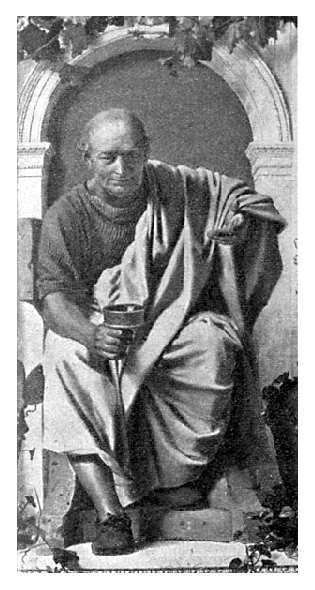
\includegraphics[width=30mm]{./img/Quintus_Horatius_Flaccus.eps}}

    \ifEnglish
      \put(80,110) {
        \begin{minipage}[c]{70mm}\scriptsize
          Quintus Horatius Flaccus\\
          BC.65.12.8--BC.8.11.27\\
          Roman poet from Southern Italy
      \end{minipage}}
    \else
      \put(80,106) {
        \begin{minipage}[c]{70mm}\scriptsize
          クィントゥス・ホラティウス・フラックス\\
          Quintus Horatius Flaccus\\
          BC.65.12.8--BC.8.11.27\\
          古代ローマ時代の南イタリアの詩人
      \end{minipage}}
    \fi
    \put(10,130){\fbox{
\includegraphics[width=60mm]{./img/Carpe_Diem.eps}}}

    \ifEnglish
      \put(10,108){
        \begin{minipage}[c]{60mm}\small
          In the sundial of the photograph, it is engraved with ``Carpe Diem'' in Latin, ``Seize the day'' in English.
          It means that you will enjoy the day and living the best.
          It is a phrase that appears in the poetry of ancient Roman poet Horatius in the 1st century BC.
          The phrase also appears in the movie ``Dead Poets Society'', 1989 played by Robin William.
      \end{minipage}}
    \else
      \put(10,100){
        \begin{minipage}[c]{60mm}\small
          　写真の日時計にはラテン語で``Carpe Diem''（カルペ・ディアム）と彫ってあります。
          英語では``Seize the day''、
          日本語では「その日を摘め」と訳されています。
          そこには「その日を楽しみ、精一杯いきること」という意味があります。
          紀元前1世紀の古代ローマの詩人ホラティウスの詩に登場する句で、
          映画``Dead Poets Society''（1989年、邦題「いまを生きる」ロビン・ウィリアムズ主演）にも出てきます。
      \end{minipage}}
    \fi

    \put(20,0){
      \begin{minipage}[c]{100mm}\small
        \begin{center}
          Ten Sentences A Day for Eight Weeks\\Dictation Everyday\\

          \textcopyright\ First edition\\

          \textcopyright 2020, Hilofumi Yamamoto
        \end{center}
    \end{minipage}}
  \end{picture}

  \newpage
  \thispagestyle{empty}
  \begin{picture}(50,160)(0,0)\centering
    \put(07, 51){\fbox{
\includegraphics[width=100mm]{./img/Carpe_Diem.eps}}}
    \put(42, 41){\Large\sc Carpe Diem}
    % \put(38, 30){\fcolorbox{white}{royalblue}{\includegraphics[width=35mm]{../phd/logo02.png}}}
%    \put(38, 30){\fbox{
\includegraphics[width=35mm]{./img/tokyotechlogo/symbol_pdf_ja_180704/シンボルマーク+ロゴタイプ和文英文左右.pdf}}}
    \put(38, 30){\fbox{
\includegraphics[width=35mm]{./img/sciencetokyo.png}}}
    \put(38, 10){
\includegraphics[trim=0 0 0 0, clip, width=38.5mm]{./img/KAKENHIlogo_M.eps}}
  \end{picture}

  \end{document}


  EEEEEEEEE
  \begin{comment}
    \subsubsection{Sentences}

    考える・考えすぎる

\ifEnglish
I'm so jaded.
\else
もううんざり。
\fi

    \begin{enumerate}
      \item 授業は隣の人とのおしゃべりが中心、
      \item 毎回振り返りのレポート、
      \item 試験問題を学生自らが作り、
      \item 鉛筆を転がすような試験ではなく、
      \item 本質が議論できるよう口述試験を受け、
      \item テーマを自分で選び、
      \item 決められた作法で書くことを学び、
      \item 自分で何かを明らかにする、
      \item 徹底的に能動的でなければ参加できない形式にした。
    \end{enumerate}

    \begin{enumerate}
      % \item motte-kuru/bring.vt\index{motte-kuru/bring.vt}/持ってくる
      \item これから先/korekara-saki/from now on/
      \item こないだ/konaida/last day/
      \item 24歳/nij\=uyon-sai/24 years old/
      \item 待たせる/mataseru/vt.causative.let-sb-wait/
      \item いつも/itsumo/always/
      \item 休み/yasumi/day-off/
      \item 人生/jinsei/life/
      \item ..はず/..hazu/think that it must ../
      \item 安心する/anshin-suru/n.suru.be-relieved/
      \item 笑顔/egao/smile/
      \item 楽しみ/tanoshimi/n.masu.fun/
      \item 早くして/hayaku-shite/i-adj.ku-shite.to-do-earlier/
      \item ta-dar\=oni../it would have been\index{..ta-dar\=oni../it would have been}/--ただろうに
      \item いくらか/ikuraka/some amount of money/
      \item 都合する/tsug\=o-suru/n-suru.prepare-sth-for-sb/
      \item 質問/shitsumon/question/
      \item 返し/kaeshi/v.masu.return/
      \item ..に来た/..ni-kita/come to do ..: GN v.masu.ni-kuru/iku/\label{212848_16Mar19}
      \item ついでに/tsuideni/in this chance/
      \item 会って/atte/vt.te.meet)$\rightarrow$会う/au/vt.meet/
      \item 帰ろう/kaer\=o/v.vol.go-home/
      \item 自分で/jibun-de/by myself/
      \item どうかな/d\=okana/how do you think about it?/
      \item 暑かった/atsukatta/i-adj.past.hot/
      \item さっぱり/sappari/n.masu.light/
      \item ..の前で/..no-mae-de/in-front-of../
      \item 緊張/kinch\=o/n.suru.be-nervous/
      \item ..しちゃった/..shi-chatta/v.te-shimau: GN/\label{193441_16Mar19}
      \item でしょ/desho/isn't it?/aren't they?/
      \item 待ってて/mattete/v.te-te: GN v.te-iru/\label{193716_16Mar19}
      \item 持ってくる/motte-kuru/vt.bring/
      \item 会えなかった/aenakatta/v.pot.past.neg: could not see sb/
      \item 方向/h\=ok\=o/direction/
      \item 向かって/mukatte/v.te.go-for/
      \item 向かう/mukau/vi.go-for/
      \item 大切な/taisetu-na/na-adj.important/precious/

      \item りんご/ringo/apple/
      \item みかん/mikan/orange/
      \item バナナ/banana/banana/
      \item などなど/nado-nado/etc.etc./
      \item えっと/etto/well/
      \item 歌って/utatte/vt.te.sing/
      \item 踊って/odotte/vi.te.dance/
      \item 飲んで/nonde/vi.te.drink/
      \item 楽しかった/tanoshikatta/i-adj.past.fun/
      \item 聞かれる/kika-reru/v.psiv.be-asked/\label{195700_16Mar19}
      \item 即答/sokut\=o/n.suru.quick-answer/
      \item なんとなく/nantonaku/somehow/
      \item 親切/shinsetsu/na-adj.kind/
    \end{enumerate}
  \end{comment}

  \subsubsection{Sentences}
  \begin{enumerate}
  \end{enumerate}

  \subsubsection{Words and Expressions}
  \begin{enumerate}
    \item ときどき/tokidoki/sometimes/
    \item 何か/nanika/something/
    \item 真剣に/shinken-ni/na-adj-ni.serious/
    \item 考えたりする/kangae-tari-suru/v.tari-suru.sometimes-think: GN v.tari-suru/\label{114509_17Mar19}
    \item うまく行かない/umaku-ikanai/not go well/
    \item 考えすぎて/kangae-sugite/think too much/
    \item ..てしまう/..te-shimau/GN cannot help doing/\label{115116_17Mar19}
    \item ..ものです/..mono-desu/we would do it usually/naturally: GN mono-da/\label{115559_17Mar19}
    \item ..わけではない/..wake dewa nai/it is not always ../
    \item わけ/wake/reason/
    \item まじめ/majime/serious/
    \item 信頼/shinrai/n.suru.psiv.te-iru.be-trusted/
    \item 建築家/kenchikuka/architect/
    \item なられた/narareta/v.honorific.be: GN/\label{120140_17Mar19}
    \item 理由/riy\=u/reason/
    \item はっきりさせる/hakkiri-saseru/make it clear/
    \item はっきりする/hakkiri/v.suru.be-clear/
    \item もともと/motomoto/originally/
    \item ヒーロー
    \item しぶい
    \item とっておきの
    \item かっこいい
    \item たのもしいなあ
    \item ロケ地発見...ですかねぇ。
  \end{enumerate}

  本当の勝負/hont\o no sh\=obu/the real challenge; the real contest/

  \section{Day 6: Greeting 2}

  \ifEnglish
    The words of greeting are different depending on the time of a day.
  \else
    時間によって、あいさつのことばはちがいます。
  \fi
  \ifEnglish
    It depends on morning, noon, evening, when going to bed, when meeting, when leaving, and so on.
  \else
    朝、昼、晩、就寝前、会った時、別れる時等によっても変わります。
  \fi
  \ifEnglish
    Let's use a variety of greeting.
  \else
    いろいろな挨拶を使ってみましょう。
  \fi

  \subsection*{Sentences}

  \begin{enumerate}
    \itemsep=5pt
    \item A: おはよう。 B: \underline{おはようございます}。\\A: Good morning. B: Good morning.%おはようございます%
    \item A: 田中さん！ B: あ、\underline{先生、こんにちは}。\\A: Mr. Tanaka. B: Hello teacher.%せんせい、こんにちは,せんせいこんにちは%
    \item A: では、また。 B: はい、では、\underline{失礼します}。\\A: Alrigh then, see you, next time. B: Now, I got to go.%しつれいします%
    \item A: 田中さん、こんにちは？ B: \underline{はい、こんにちは}。\\A: Hello, Mr. Tanaka B: Hi, hello!%はい、こんにちは,はいこんにちは%
    \item A: 本田先生、こんばんは？ B: \underline{はい、こんばんは}。\\A: Hello, Professor HondaB: Hi, hello!%はい、こんばんは,はいこんばんは%

    \item A: さようなら。B: では、\underline{しつれいします}。\\A: Good bye B: Pardon me, I have to go now.%しつれいします%
    \item A: 夜遅くまでどうもありがとう。 B: こちらこそ。\underline{おやすみなさい}。\\A: Thank you very much for attending by late night B: Thank YOU. Good night.%おやすみなさい%
    \item A: こんにちは。お元気ですか。 B: はい、\underline{げんきです}。\\A: Hello, how are you? B: Yes, I am fine.%げんきです%
    \item A: 本田先生、毎日、あついですね。 B: そう、\underline{あついね}。\\A: Professor Honda, it's very hot everyday, isn't it? B: Yes, it is.%あついね%
    \item A: ねえ、元気？ B: 元気だけど、\underline{ちょっとさむい}。\\A: Hey, are you all fine? B: I am fine, but it's too cold.%ちょっとさむい%
  \end{enumerate}

  \subsection*{Words and Expressions}


%D4E%]

  \chapter{Introduction}

  \ifEnglish
    \section{Development policy}
  \else
    \section{開発方針}
  \fi

  \ifEnglish
    \subsection*{Question data}
    \begin{enumerate}
      \item Collecting over 500 sentences for 50 days.
      \item Attaching English translation to all sentences.
      \item Incorporating colloquial conversation expressions and slangs.
    \end{enumerate}

  \else
    \subsection*{設問データ}
    \begin{enumerate}
      \item 日常口語表現を500文50日分を収録。
      \item すべての文には英語訳をつける。
      \item 口語表現、俗語をふんだんに取り入れる。
    \end{enumerate}

  \fi

  \ifEnglish
    \subsection*{Screen creation}
    \begin{enumerate}
      \item In the commentary, a teacher writes sentences which explain the minimum essentials on paper with a pencil and makes a video to state the necessary points.
      \item Make the same way as for TV telop.
      \item In practice, show TV telop a number of times.
      \item Let me write words and kana seen on TV telop.
      \item Turn off the television telop and write the words and kana seen just before.
      \item Show the part that matches all or part of the question and underline it otherwise.
    \end{enumerate}

  \else
    \subsection{画面作成}
    \begin{enumerate}
      \item 解説は、教師が鉛筆で紙に文字を書いて、必要最小限の要点を述べるをビデオを作る。
      \item テレビテロップと同様の作り方をする。
      \item 練習ではテレビテロップを何度も見せる。
      \item テレビテロップに見られた単語やかなを書かせる。
      \item テレビテロップを消して、直前に見た単語やかなを書かせる。
      \item 設問は全部・一部一致したところを見せて、それ以外をアンダーラインにする。
    \end{enumerate}

  \fi

  \ifEnglish
    \subsection*{Grading}
    \begin{enumerate}
      \item Set difficulty level for questions.
      \item The difficulty level of the question is based on the length of the sentence.
      \item Terminology notes and grammar notes relating to questions are fulfilled as appropriate.
    \end{enumerate}

  \else
    \subsection*{難易度}
    \begin{enumerate}
      \item 設問に難易度をつける。
      \item 設問の難易度は文の長さを基本とする。
      \item 設問に関連する用語ノート、文法ノートは適宜充実させる。
    \end{enumerate}

  \fi

  \ifEnglish
    \subsection*{Question pace}
    \begin{enumerate}
      \item Over 50 dictations per week.
      \item Perform a dictation of over 300 questions in total for 6 weeks.
      \item Review items with low correct answer rate.
      \item Review items that have not been implemented for a while even if you answer correctly.
      \item If review is correct answer rate 100, we will not make a further test.
    \end{enumerate}

  \else
    \subsection*{設問ペース}
    \begin{enumerate}
      \item 1週間に70文のディクテーションを行う。
      \item 8週間計500文のディクテーションを行う。
      \item 正答率の低いものを復習する。
      \item 正答してもしばらく実施していない項目は復習する。
      \item 復習が正答率100であれば、もう出題しない。
    \end{enumerate}

  \fi

  \ifEnglish
    \subsection*{Completion test}
    \begin{enumerate}
      \item Test only 100 with low correct answer rate.
      \item Pass the exam at 90%.
    \end{enumerate}

  \else
    \subsection*{修了試験}
    \begin{enumerate}
      \item 正答率が低いもののみを100テストする。
      \item 90％で合格にする。
    \end{enumerate}

  \fi

  \begin{comment}
    \ifEnglish
      \href{https://basic.system5.jp/archives/514}{Telop is the third kind of word! Its importance}
    \else
      \href{https://basic.system5.jp/archives/514}{テロップは第3のコトバ！その重要性}
    \fi
  \end{comment}

  \ifEnglish
    \subsection*{Study with a mobile terminal}
    \begin{enumerate}
      \item Design to be able to take on mobile terminals.
    \end{enumerate}

  \else
    \subsection*{携帯端末での履修}
    \begin{enumerate}
      \item 携帯端末で履修できるように設計する。
    \end{enumerate}


    \ifEnglish
      \section{Procedure}
      \begin{enumerate}
        \item Listen to sentences
        \item Type what one heard
        \item Rating (automatic scoring)
        \item Review (Incorrect Question Review)
      \end{enumerate}

    \else
      \section{手順}
      \begin{enumerate}
        \item 文を聞く
        \item 聞こえた文をタイプする
        \item 採点（自動採点）
        \item 復習（誤った問を復習）
      \end{enumerate}
    \fi

    \ifEnglish
      \section{Question after dictation practice}
      \begin{enumerate}
        \item Which was a difficult dictation?
        \item What was difficult?
        \item Let's write the sentence of successful dictation again.
      \end{enumerate}

    \else
      \section{ディクテーション練習後の質問}
      \begin{enumerate}
        \item むずかしかったディクテーションはどれでしたか。
        \item \ruby{何}{なに}がむずかしかったのですか。
        \item うまくできたディクテーションの\ruby{文}{ぶん}をもういちど\ruby{書}{か}いてみましょう。
      \end{enumerate}
    \fi

    \ifEnglish
      \subsection{Day 16x: Something tedious}%E
    \else
      \subsection{Day 16x: 面倒なこと}%J
    \fi

    \subsubsection{Sentences}
    \subsubsection{Words and Expressions}

%%%%%%%%<ruby><rb>  </rb><rp>(</rp><rt>  </rt><rp>)</rp></ruby>
%%%%%%%%\hspace{6em}
%%%%%%%%\ruby{}{}
%%%%%%%%\mySound{14401}
%%%%%%%%<BLANK>
\ifWB
\else
\fi%WB
%D4E%ID:
%D4E%sentence:
%D4E%english:
%D4E%answer:
%D4E%model:
%D4E%roman:
%D4E%notes:
